\documentclass{unina_doc_class}
\pgfplotsset{compat=1.18}
\gdef\documentname{Algebra}
\gdef\documentyear{A.A\ 2023-2024}
\gdef\xauthors{\href{giorgio99difusco@gmail.com}{\hi{\iuser Giorgio Di Fusco}}}
\gdef\yauthors{Mario Majorano, Andrea Di Donato, Luigi Ruggiero, Luigi Ferrara}
\pagestyle{plain}
\begin{document}
 \coverpage{26}{\documentyear}{30}{\documentname}
  % Chapter 0: Introduction
  \chapter{Introduzione}
\introduction{G. Cutolo}{}

\newpage

\section{Sulle versioni del documento}

\warning{Attento}{
	\textbf{Esistono diverse versioni di questo documento in circolazione}. È fondamentale assicurarsi di \textbf{consultare sempre la versione più recente}, in quanto potrebbe contenere informazioni aggiornate o correzioni rispetto alle versioni precedenti. Per evitare di studiare da fonti non esatte si raccomanda vivamente di verificare la data di pubblicazione e il numero di revisione riportati alla fine di questa pagina.
}

\begin{minipage}{.45\textwidth}
	\begin{center}
		\begin{tblr}{
			colspec = {c|c},
			hlines,
			vlines,
			row{1} = {font=\bfseries, primary!80},
			width = \linewidth
		}
		Revisione & Data \\
		\SetRow{red9} 67dfc7c & 15/03/2024 \\
		\SetRow{red9} 00a8221 & 28/08/202 \\
		\SetRow{red9} 343cc71 & 29/08/2024  \\
		\SetRow{red9}9087dcf & 11/09/2024  \\
		\SetRow{yellow9} 83a3f0f & 01/10/2024 \\
		\SetRow{yellow9} 3af1354 & 19/02/2025 \\
		\SetRow{green9}  3d59ec1 & 05/09/2025
	\end{tblr}
	\captionof{table}{Cronologia revisioni del documento}
	\end{center}
\end{minipage}
\hfil
\begin{minipage}{.45\textwidth}
	\begin{center}
		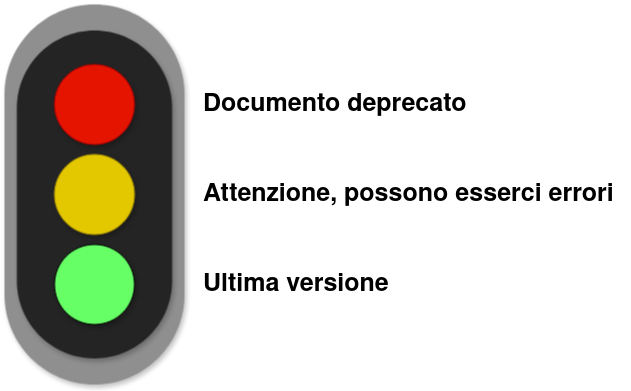
\includegraphics[scale=.35]{sources/Semaforo.drawio}
	\end{center}
\end{minipage}


\section{Repository del progetto}
Tutte le versioni del documento, insieme al codice sorgente e ai materiali aggiuntivi, sono disponibili nella \href{https://github.com/Giordi9902/unina_algebra_notes}{repository} ufficiale su GitHub.

Ti invitiamo a consultare la repository per eventuali aggiornamenti, contributi o per segnalare problemi direttamente tramite issue.

\subsection{In caso di errori}
È sempre ben gradito ricevere feedback.

\textbf{Feedback generali:} se hai domande rispetto qualsiasi aspetto del libro non esitare a contattarmi:
\begin{itemize}
	\item Email: \texttt{giorgio99difusco@gmail.com}
\end{itemize}

  % Chapter 1: Logica
  \tableofcontents
  \chapter{Logica rudimentale}

\section{Proposizioni logiche}
Ogni teoria matematica è espressa in un \textbf{linguaggio}, che è costituito da:
\begin{enumerate}
	\item Da un \textbf{alfabeto di simboli} che possono essere messi insieme per costruire parole (stringhe di caratteri);
	\item Da \textbf{regole sintattiche} che permettono di distinguere tra stringhe ``composte correttamente'', chiamate \textbf{formule}, e stringhe che non sono correttamente composte.
\end{enumerate}

\begin{example}
	Ad esempio, la stringa ``$0<1$'' rappresenta una formula mentre la stringa $``0<$'' no.
\end{example}
Tra le formule matematiche facciamo un'ulteriore distinzione: 

\dfn{Formula chiusa}{
	Le formule alle quali è possibile attribuire univocamente un valore di verità, \textit{vero} o \textit{falso}, vengono chiamate \textbf{proposizioni} o \textbf{formule chiuse}\index{Formula chiusa}.
}

\begin{example}
	La formula ``$x>1$'' non è una proposizione in quanto non possiamo associare un valore vero o falso in quanto \textit{dipendente} dal valore della variabile $x$.
\end{example}
\subsection{I connettivi logici}
Ogni linguaggio contiene dei simboli, mediante i quali è possibile costruire periodi più complessi a partire da blocchi atomici. Anche nella logica matematica esistono dei simboli, chiamati \textbf{connettivi logici}\index{Connettivi}, che permettono di costruire proposizioni più complesse a partire da proposizioni più semplici. I connettivi logici più comuni sono:
\begin{itemize}
	\item \textbf{Negazione}: $\neg$;
	\item \textbf{Congiunzione}: $\land$;
	\item \textbf{Disgiunzione}: $\lor$;
	\item \textbf{Disgiunzione esclusiva}: $\xor$;
	\item \textbf{Equivalenza}: $\iff$;
	\item \textbf{Implicazione}: $\implies$.
\end{itemize}
\subsubsection{Negazione}\index{Connettivi!Negazione}
La negazione di una proposizione $p$ è una proposizione che è vera quando $p$ è falsa e viceversa. La negazione di una proposizione $p$ viene indicata con $\neg p$. Il connettivo di negazione è \textbf{unario}, ovvero è un connettivo che agisce su una sola proposizione. Spesso, per visualizzare i valori di verità di una proposizione, si utilizza una tabella chiamata \textbf{tabella di verità}. 

La tabella di verità della negazione è la seguente:

\begin{center}
	\begin{tblr}{
			hlines = {0.9pt}, vlines = {0.9pt}, colspec = {X[c]X[c]X[c]},
			row{1} = {primary!80!white}}
		$p$ & $\neg p$ \\
		V & F \\
		F & V
	\end{tblr}
	\captionof{table}{Tavola di verità della negazione}\label{tab:negation}
\end{center}

\subsubsection{Congiunzione}\index{Connettivi!Congiunzione}
La congiunzione di due proposizioni $p$ e $q$ è una proposizione che è vera quando $p$ e $q$ sono vere e falsa in tutti gli altri casi. La congiunzione di due proposizioni $p$ e $q$ viene indicata con $p \land q$. Il connettivo di congiunzione è \textbf{binario}, ovvero è un connettivo che agisce su due proposizioni. La tabella di verità della congiunzione è la seguente:

\begin{center}
	\begin{tblr}{
			hlines = {0.9pt}, vlines = {0.9pt}, colspec = {X[c]X[c]X[c]},
			row{1} = {primary!80!white}}
		$p$ & $q$ & $p \land q$ \\
		V & V & V \\
		V & F & F \\
		F & V & F \\
		F & F & F
	\end{tblr}
	\captionof{table}{Tavola di verità della congiunzione}\label{tab:congiunzione}
\end{center}

\subsubsection{Disgiunzione}\index{Connettivi!Disgiunzione}
La disgiunzione di due proposizioni $p$ e $q$ è una proposizione che è vera quando $p$ o $q$ sono vere e falsa in tutti gli altri casi. La disgiunzione di due proposizioni $p$ e $q$ viene indicata con $p \lor q$. La tabella di verità della disgiunzione è la seguente:

\begin{center}
	\begin{tblr}{
			hlines = {0.9pt}, vlines = {0.9pt}, colspec = {X[c]X[c]X[c]},
			row{1} = {primary!80!white}}
		$p$ & $q$ & $p \lor q$ \\
		V & V & V \\
		V & F & V \\
		F & V & V \\
		F & F & F
	\end{tblr}
	\captionof{table}{Tavola di verità della disgiunzione}\label{tab:disgiunzione}
\end{center}

\subsubsection{Disgiunzione esclusiva}\index{Connettivi!Disgiunzione esclusiva}
La disgiunzione esclusiva di due proposizioni $p$ e $q$ è una proposizione che è vera quando $p$ o $q$ sono vere, ma non entrambe, e falsa in tutti gli altri casi. La disgiunzione esclusiva di due proposizioni $p$ e $q$ viene indicata con $p \xor q$. La tabella di verità della disgiunzione esclusiva è la seguente:

\begin{center}
	\begin{tblr}{
			hlines = {0.9pt}, vlines = {0.9pt}, colspec = {X[c]X[c]X[c]},
			row{1} = {primary!80!white}}
		$p$ & $q$ & $p \xor q$ \\
		V & V & F \\
		V & F & V \\
		F & V & V \\
		F & F & F
	\end{tblr}
	\captionof{table}{Tavola di verità della disgiunzione esclusiva}\label{tab:xor}
\end{center}

\subsubsection{Equivalenza}\index{Connettivi!Equivalenza}
L'equivalenza di due proposizioni $p$ e $q$ è una proposizione che è vera quando $p$ e $q$ hanno lo stesso valore di verità e falsa in tutti gli altri casi. L'equivalenza di due proposizioni $p$ e $q$ viene indicata con $p \iff q$. La tabella di verità dell'equivalenza è la seguente:

\begin{center}
	\begin{tblr}{
			hlines = {0.9pt}, vlines = {0.9pt}, colspec = {X[c]X[c]X[c]},
			row{1} = {primary!80!white}}
		$p$ & $q$ & $p \iff q$ \\
		V & V & V \\
		V & F & F \\
		F & V & F \\
		F & F & V \\
	\end{tblr}
	\captionof{table}{Tavola di verità dell'equivalenza logica}\label{tab:equivalence}
\end{center}

\begin{defbox}{Proposizione logica}\index{Proposizione}
	Una \textbf{proposizione logica} o \textbf{forma proposizionale} è una formula ottenuta dalla composizione di una o più formule mediante connettivi logici.
\end{defbox}

Per calcolare il valore di verità di una forma proposizionale possiamo avvalerci delle tabelle di verità oppure, come si vedrà più in avanti, usare alcune proprietà che permettono di arrivare al risultato in maniera più veloce. Infatti, data una forma proposizionale di $k$ variabili è necessario costruire una tabella di $2^{k}$ righe.

\begin{example}
	\begin{enumerate}
	\item Si voglia calcolare il valore di verità della forma $p \land (q \lor p)$, dove $p$ e $q$ sono proposizioni. La tabella di verità conterrà $2^{2}=4$ righe e sarà la seguente:
	\begin{center}
		\begin{tblr}{
				hlines = {0.9pt}, vlines = {0.9pt}, colspec = {X[c]X[c]X[c]X[c]}, cells={mode=math},
				row{1} = {primary!80!white}}
			p & q & q \lor p & p \land (q \lor p)\\
			V & V & V & V \\
			V & F & V & V \\
			F & V & V & F \\
			F & F & F & F
		\end{tblr}
	\end{center}
	
	Come si può notare, per calcolare il valore di verità della formula finale ci siamo avvalsi di una colonna intermedia.


	\item Si calcoli il valore di verità della forma $P \land (Q \lor R)$, dove $P$, $Q$ e $R$ sono proposizioni. Essendo tre le variabili proposizionali la tabella di verità avrà $2^{3}=8$ righe.
	\begin{center}
		\begin{tblr}{
				hlines = {0.9pt}, vlines = {0.9pt}, colspec = {X[c]X[c]X[c]X[c]X[c]}, cells={mode=math},
				row{1} = {primary!80!white}}
			p & q & r & q \lor r & p \land (q \lor r)\\
			V & V & V & V & V \\
			V & F & V & V & V \\
			F & V & V & V & F \\
			F & F & V & V & F \\
			V & V & F & V & V \\
			V & F & F & F & F \\
			F & V & F & V & F \\
			F & F & F & F & F
		\end{tblr}
	\end{center}

	\item Un altro esempio banale di proposizioni logicamente equivalenti è dato dalla formula $P \land P$ e $P$. Si vede infatti immediatamente dalla tabella di verità:
	
	\begin{center}
		\begin{tblr}{
				hlines = {0.9pt}, vlines = {0.9pt}, colspec = {X[c]X[c]X[c]},
				row{1} = {primary!80!white}}
			$P$ & $P \land P$ & $P \iff P \land P$\\
			V  & V & V \\
			F  & F & V
		\end{tblr}
	\end{center}
	Osservando la tavola di verità notiamo che la prima e l'ultima colonna sono uguali. Questo è dovuto al fatto che la congiunzione è un connettivo \textbf{idempotente}, ovvero che restituisce sempre il primo valore di verità quando le due proposizioni sono uguali. 
\end{enumerate}
\end{example}

\begin{defbox}{Tautologia}\index{Tautologia}
	Una forma proposizionale $\varphi$ che assume valore di verità vero in modo del tutto indipendente dai valori attribuiti alle variabili che appaiono in $\varphi$ viene chiamata \textbf{tautologia}. Dualmente, esistono forme proposizionali $\varphi$ per le quali, calcolato il valore di verità, si ottiene sempre il valore F. Queste si chiamano \textbf{contraddizioni}.
\end{defbox}

Ovviamente $\varphi$ è una contraddizione se e solo se $\neg \varphi$ è una tautologia. Una forma proposizionale che non sia né una tautologia né una contraddizione si dice \textbf{contingente}. Le tautologie sono molto utili nelle dimostrazioni. Infatti, nota la tabella di verità di una determinata formula siamo in grado di sapere la tabella di verità di una formula logicamente equivalente alla prima.

\begin{example}
\begin{enumerate}
	\item La \textbf{doppia negazione} è una tautologia. Infatti, la tabella di verità è la seguente:
	
	\begin{center}
		\begin{tblr}{
				hlines = {0.9pt}, vlines = {0.9pt}, colspec = {X[c]X[c]X[c]},
				row{1} = {primary!80!white}}
			$p$ & $\neg p$ & $\neg (\neg p)$\\
			V & F & V \\
			F & V & F
		\end{tblr}
	\end{center}
	
	La doppia negazione è molto utile per semplificare le formule proposizionali. Infatti, è possibile semplificare la formula $P \land \neg (\neg P)$ in $P \land P$ e quindi in $P$.

	\item Il \textbf{principio di non contraddizione} afferma che una proposizione non può essere vera e falsa allo stesso tempo. Questo principio può essere espresso in logica proposizionale come $\neg (p \land \neg p)$, ovvero la negazione della congiunzione di una proposizione e della sua negazione. La tabella di verità è la seguente:
	
	\medskip
	
	\begin{center}
		\begin{tblr}{
				hlines = {0.8pt}, vlines = {0.9pt}, colspec = {X[c]X[c]X[c]X[c]},
				row{1} = {primary!80!white}}
			$p$ & $\neg p$ & $p \land \neg p$ & $\neg (p \land \neg p)$\\
			V & F & F & V \\
			F & V & F & V \\
		\end{tblr}
	\end{center}
	\medskip
	
	Come si può notare, la formula è una tautologia. Analogamente, è possibile ottenere una tautologia simile utilizzando il connettivo di disgiunzione: $p \lor (\neg p)$. Esempi di questa proposizione nel parlato quotidiano possono essere: ``In questo momento piove oppure in questo momento non piove'', ``Studio l'algebra oppure non studio l'algebra'', ecc. Verità oggettive sotto qualsiasi punto di vista.
\end{enumerate}
\end{example}

\begin{propbox}
	Siano $P$ e $Q$ due forme proposizionali. $P$ e $Q$ sono logicamente equivalenti se e solo se $ (P \iff Q)$ è una tautologia.
\end{propbox}

\begin{proof}
	Banale. Siano $P$ e $Q$ due proposizioni logicamente equivalenti, si ha allora:
	\begin{center}
		\begin{tblr}{hlines,vlines,row{1}={primary!80!white},colspec={X[c]X[c]X[c]},cells={mode=math}}
			P & Q & P \iff Q \\
			V & V & V \\
			F & F & V
		\end{tblr}
	\end{center}
	e  $P \iff Q$ risulta essere quindi una tautologia. Viceversa, sia $P \iff Q$ una tautologia. Allora, per definizione di equivalenza logica, $P$ e $Q$ hanno gli stessi valori logici e quindi sono logicamente equivalenti.
\end{proof}

\subsection{Il connettivo condizionale}\index{Connettivi!Implicazione}
Il connettivo condizionale è un connettivo binario che associa due proposizioni $p$ e $q$ e restituisce una proposizione che è falsa quando $p$, detta ``antecedente'', è vera e $q$, detta ``conseguente'', è falsa, e vera in tutti gli altri casi. Il connettivo condizionale di due proposizioni $p$ e $q$ viene indicato con $p \implies q$. Il connettivo condizionale è anche detto \textbf{implicazione}. La tabella di verità del connettivo condizionale è mostrata nella Tabella \ref{tab:condizionale}.

\begin{center}
	\begin{tblr}{
			hlines = {0.9pt}, vlines = {0.9pt}, colspec = {X[c]X[c]X[c]},
			row{1} = {primary!80!white}}
		$p$ & $q$ & $p \implies q$ \\
		V & V & V \\
		V & F & F \\
		F & V & V \\
		F & F & V
	\end{tblr}
	\captionof{table}{Tavola di verità del connettivo condizionale.}\label{tab:condizionale}
\end{center}

\begin{example}
	Nella logica proposizionale, frasi come ``Se piove allora il Vesuvio è alto più di mille metri sul livello del mare'' hanno assolutamente senso in quanto sono delle vere e proprie formule proposizionali. Infatti, se indichiamo con $P$ la proposizione ``piove'' e con $Q$ la proposizione ``il Vesuvio è alto più di mille metri sul livello del mare'', la frase precedente può essere riscritta come $P \implies Q$.
\end{example}

\begin{osservation}
	Perché le implicazioni con antecedente falso devono essere vere? Consideriamo la frase: ``Per ogni numero intero $x$ compreso tra 1 e 3 si ha che se $x>2$ allora $x>1$''. Tutti concordiamo sul fatto che questa frase sia vera. Analizziamola: essa significa che tutte le implicazioni del tipo $x>2 \implies x>1$ ottenute sostituendo ad $x$ uno dei numeri 1, 2, 3 sono vere. Sono vere quindi le proposizioni:
	\begin{enumerate}[itemjoin={,\quad}]
		\item $\Phi_{1}$: ``$1>2 \implies 1>1$''
		\item $\Phi_{2}$: ``$2>2 \implies 2>1$''
		\item $\Phi_{3}$: ``$3>2 \implies 3>1$''
	\end{enumerate}
	In particolare risulta vera anche la proposizione $\Phi_{1}$, che è del tipo $F \implies V$. Questo è in accordo con la tabella di verità del connettivo condizionale (Tabella \ref{tab:condizionale}). Dunque le implicazioni con antecedente falso sono vere. Si osserva che sono vere anche le implicazioni con conseguente vero. In effetti, si può dire, sinteticamente, che una \textit{implicazione è vera precisamente quando il suo antecedente è falso o il suo conseguente è vero}.
\end{osservation}

\section{Proprietà dei connettivi logici}\label{proprietà_connettivi}
Esprimere una proprietà per un connettivo logico significa affermare che la tabella di verità di una formula è sempre uguale a quella di un'altra formula. In altre parole, significa affermare che le due formule sono logicamente equivalenti e quindi che la formula che esprime la proprietà è una tautologia.

\begin{propbox}
	I connettivi logici godono delle seguenti proprietà, valgono cioè le seguenti tautologie:
	\begin{enumerate}
		\item \textbf{Idempotenza:}
		\begin{eqnarray}
			p \land p &\iff& p \\
			p \lor p &\iff& p
		\end{eqnarray}
		\item \textbf{Commutatività:}
		\begin{eqnarray}
			p \land q &\iff& q \land p \\
			p \lor q &\iff& q \lor p \\
			p \xor q &\iff& q \xor p \\
			\bigl(p \iff q\bigr) &\iff& \bigl(q \iff p\bigr)
		\end{eqnarray}
		\item \textbf{Associatività}
		\begin{eqnarray}
			\bigl(p \land q\bigr) \land r &\iff& p \land \bigl(q \land r\bigr)\\
			\bigl(p \lor q\bigr) \lor r &\iff& p \lor \bigl(q \lor r\bigr)\\
			\bigl((p \iff q) \iff r\bigr) &\iff& \bigl(p \iff (q \iff r)\bigr) \label{eq:associativity_logical_equivalence}
		\end{eqnarray}
		\item \textbf{Distributività:}
		\begin{eqnarray}
			\bigl(p \land (q \lor r)\bigr) \iff \bigl((p \land q) \lor (p \land r)\bigr)\\
			\bigl(p \lor (q \land r)\bigr) \iff \bigl((p \lor q) \land (p \lor r)\bigr)
		\end{eqnarray}
	\end{enumerate}
\end{propbox}

\begin{proof}
	Per esercizio mostriamo la dimostrazione della proprietà associativa dell'equivalenza logica (\ref{eq:associativity_logical_equivalence}). La dimostrazione delle altre proprietà è lasciata al lettore. La verifica del fatto che la proprietà in questione si tratti di una tautologia è immediata se si osserva la tabella di verità \ref{tab:associativity_equivalence}.
	
	\begin{center}
		\begin{tblr}{
				hlines = {0.9pt}, vlines = {0.9pt}, colspec = {X[c]X[c]X[c]X[c]X[2,c]X[2,c]},
				row{1} = {primary!80!white}}
			$p$ & $q$ & $r$ & $p \iff q$ & $(p \iff q) \iff r$ & $p \iff (q \iff r)$ \\
			V & V & V & V & V & V \\
			V & V & F & V & V & V \\
			V & F & V & F & F & F \\
			V & F & F & F & F & F \\
			F & V & V & F & F & F \\
			F & V & F & F & F & F \\
			F & F & V & V & V & V \\
			F & F & F & V & V & V
		\end{tblr}
		\captionof{table}{}\label{tab:associativity_equivalence}
	\end{center}
	
	Si noti che $((p \iff q)\iff r)$ risulta vera se e solo se esattamente uno o tutti e tre tra $p$, $q$ ed $r$ risulta vera. 
\end{proof} 

\begin{osservation}
	Sull'associatività di $\land$ e $\lor$, si osserva che $(p\land q)\land r$ risulta vera se e solo se sono contemporaneamente vere sia $p$ che $q$ che $r$ (lo stesso vale per $r \land (q \land r)$), mentre $(p \lor q)\lor r$ è vera se e solo se è vera almeno una tra $p$, $q$ ed $r$.
	\smallskip
	
	Più in generale è possibile provare che, qualunque sia l'intero positivo $k$ le forme proposizionale in cui appaiano tutte e sole le variabili $p_{1}, p_{2}, ..., p_{k}$, delle parentesi e, tra i connettivi solo $\land$ (analogamente $\lor$) sono equivalenti tra loro. Per queste forme si può allora rinunciare all'uso delle parentesi e scrivere semplicemente: $$p_{1} \land p_{2} \land p_{3} \land ... \land p_{k}$$ oppure $$\bigwedge_{i=1}^{k}p_{i}$$ per indicare una qualunque di queste forme.
\end{osservation}

\subsection{Le leggi di De Morgan}\index{De Morgan}
Quando è che una proposizione della forma $p \land q$ è falsa? Quando (e solo quando) è falsa almeno una tra $p$ e $q$. Questo è evidente dalla tavola di verità che descrive la congiunzione. Dualmente una proposizione della forma $p \lor q$ è falsa precisamente quando sia $p$ che $q$ sono false. Tutto questo è espresso da due tautologie molto importanti, note come \textbf{leggi di De Morgan}.

\begin{propbox}[Leggi di De Morgan]	Siano $p, \ q$ due formule, valgono allora le seguenti tautologie:
	\begin{eqnarray}
		\neg (p \land q) &\iff& (\neg p) \lor ( \neg q) \\
		\neg (p \lor q) &\iff& (\neg p) \land (\neg q)
	\end{eqnarray}
\end{propbox}

\begin{proof}
	Poniamo $\alpha \coloneqq (\neg p) \land (\neg q)$, $\beta \coloneqq (\neg p) \lor (\neg q)$. Abbiamo allora:
	\begin{center}
		\begin{tblr}
			{
				hlines = {0.9pt},
				vlines = {0.9pt},
				cells={mode=math},
				row{1}={primary!80!white},
				colspec={X[c]X[c]X[c]X[c]X[c]X[c]X[c]X[c]}
			}
			p & q & p \land q & p \lor q & \neg(p \land q) &\neg(p \lor q)& \alpha & \beta \\
			V & V & V & V & F & F & F & F\\
			V & F & F & V & V & F & F & V\\
			F & V & F & V & V & F & F & V\\
			F & F & F & F & V & V & V & V
		\end{tblr}
	\end{center}
	Dunque, per negare una disgiunzione si negano i due termini che stiamo disgiungendo e, contemporaneamente, si scambiano tra loro i simboli $\lor$ e $\land$. La negazione di una congiunzione è duale. 
\end{proof}

\subsection{Le tautologie dell'implicazione}

\begin{propbox}[Tautologia della doppia implicazione]\label{prop:doppia_implicazione}
	La congiunzione di una implicazione e della corrispondente inversa equivale alla doppia implicazione. Vale cioè la tautologia:
	\begin{equation}
		(P \iff Q) \iff \bigl((P \implies Q) \land (P \impliedby Q)\bigr)
	\end{equation}
\end{propbox}

\begin{proof} È facile convincersi osservando la seguente tabella di verità:
	\begin{center}
		\begin{tblr}
			{
				hlines = {0.9pt},
				vlines = {0.9pt}, 
				colspec = {X[c]X[c]X[c]X[c]X[c]X[2,c]},
				row{1} = {primary!80!white}, 
				cells={mode=math}
			}
			p & q & p \iff q & p \implies q & p \impliedby q & (p \implies q) \land (p \impliedby q) \\
			V & V & V & V & V & V \\
			V & F & F & F & V & F \\
			F & V & F & V & F & F \\
			F & F & V & V & V & V
		\end{tblr}
	\end{center}
	che dimostra l'enunciato.
\end{proof}

\begin{osservation}\label{oss:condizionenecessariasufficiente}
	Affermare che una certa proposizione $A$ \textbf{implica} una determinata proposizione $B$ è equivalente a dire che $A$ è una \textbf{condizione sufficiente} per $B$, ovvero che la veridicità di $A$ è sufficiente per garantire la veridicità di $B$. Inoltre, affermare che $A$ implichi $B$, è equivalente a dire che $B$ è una \textbf{condizione necessaria} per $A$, ovvero che la veridicità di $B$ è necessaria per garantire la veridicità di $A$. Il connettivo $ \implies $, a differenza degli altri connettivi binari, non è commutativo. Vale a dire che le forme $P \implies Q $ e $Q \implies P$ non sono equivalenti tra di loro.
\end{osservation}

\begin{center}
	\begin{tblr}
		{
			hlines = {0.9pt},
			vlines = {0.9pt},
			colspec = {X[c]X[c]X[c]X[c]},
			row{1} = {primary!80!white},
			row{2-5}={white},
			cells={mode=math}
		}
		P & Q & P \implies Q & Q \implies P \\
		V & V & V & V \\
		V & F & F & F \\
		F & V & V & F \\
		F & F & V & V
	\end{tblr}
	\captionof{table}{Tavola di verità dell'implicazione inversa}\label{tab:impliedby}
\end{center}

Spesso si scrive ``$P \impliedby Q$'' per ``$Q \implies P$''. Si può considerare questo simbolo ``$\impliedby$'' come un ulteriore connettivo binario (\textbf{implicazione inversa}), definito appunto dall'essere $p \impliedby q$ logicamente equivalente a $q \implies p$  come mostrato nella Tabella \ref{tab:impliedby}

\begin{example}
	Consideriamo le frasi $p:$``Oggi sto sciando'' e $q:$``Oggi sono in montagna''. Date queste due proposizioni possiamo considerare l'implicazione: ``Se oggi sto sciando allora sono in montagna.'' Questa implicazione è vera, infatti lo stare in montagna è una \textbf{condizione necessaria}\index{Condizione!Necessaria} per poter sciare ma non una condizione sufficiente. Viceversa, lo stare sciando è una \textbf{condizione sufficiente}\index{Condizione!Sufficiente} per dirci che si sta in montagna. Non vale però la formula $q \implies p$. Stare in montagna, infatti, non è sufficiente per affermare che si sta sciando, potrei infatti essere in montagna per fare una passeggiata o per fare escursionismo.
\end{example}

In generale, quando valgono contemporaneamente le formule ``$(p \implies q) \land (p \impliedby q)$'' possiamo parlare di \textbf{condizioni necessarie e sufficienti}.

\begin{center}
	\begin{tblr}
		{
			hlines = {0.9pt},
			vlines = {0.9pt},
			colspec = {X[c]X[c]X[c]},
			row{1} = {primary!80!white}
		}
		$P \implies Q$ & $P \impliedby Q$ & $P \iff Q$ \\
		Se $p$ allora $q$ & Se $q$ allora $p$ & $p$ se e solo se $q$ \\
		$p$ solo se $q$ & $p$ se $q$ & $p$ è condizione necessaria e sufficiente per $q$ \\
		$p$ è condizione sufficiente per $q$ & $p$ è condizione necessaria per $q$&$q$  è condizione necessaria e sufficiente per $p$
	\end{tblr}
	\captionof{table}{Le seguenti frasi traducono la formula nell'intestazione}
\end{center}

\begin{propbox}[Implicazione come disgiunzione]
	Il connettivo condizionale può essere espresso in termini di altri connettivi. Infatti, vale la seguente tautologia:
	\begin{equation}\label{eq:implicazione_disgiunzione}
		(p \implies q) \iff \neg p \lor q
	\end{equation}
	che esprime l'implicazione mediante la disgiunzione tra la negazione dell'antecedente e il conseguente.
\end{propbox}

\begin{proof}
	La dimostrazione segue direttamente dalle tavole di verità di implicazione e disgiunzione:
	\begin{center}
		\begin{tblr}{
				hlines = {0.9pt}, vlines = {0.9pt}, colspec ={X[c]X[c]X[c]X[c]X[c]},
				row{1} = {primary!80!white},cells={mode=math}}
			p & q & (\neg p) \lor q & p \implies q \\
			V & V & V & V \\
			V & F & F & F \\
			F & V & V & V \\
			F & F & V & V
		\end{tblr}
	\end{center}
	
	Una implicazione infatti è vera se e solo se il suo antecedente è falso o il suo conseguente è vero. 
\end{proof}

Da questa tautologia se ne può facilmente dedurre un'altra, la \hypertarget{contrapposizione}{\textbf{legge di contrapposizione}}.

\begin{propbox}[Legge di contrapposizione]\index{Contrapposizione}
	Siano $p,q$ due proposizioni logiche, vale allora la seguente:
	\begin{equation}
		(p \implies q) \iff (\neg q \implies \neg p)
	\end{equation}
\end{propbox}

\begin{proof}
	Il passaggio è il seguente:
	
	\begin{align*}
		p \implies q &\iff (\neg p) \lor q & \text{\textcolor{gray}{(per la tautologia precedente)}}  \\
		&\iff q \lor (\neg p) & \text{\textcolor{gray}{(per la commutatività di $\lor$)}} \\
		&\iff \neg(\neg q) \lor (\neg p) & \text{\textcolor{gray}{(per la doppia negazione)}} \\
		&\iff \neg q \implies \neg p & \text{\textcolor{gray}{(per la tautologia precedente)}}
	\end{align*}
\end{proof}

\begin{osservation}
	La legge di contrapposizione sta alla base del ragionamento per assurdo. Se, negando la tesi, si riesce infatti a dimostrare un fatto che neghi l'ipotesi iniziale (un \textbf{assurdo}) si dimostra allora l'implicazione originale.
\end{osservation}

Altra tautologia importante è quella che mostra come negare una implicazione. Una implicazione, infatti, è falsa precisamente quando l'\textit{antecedente è vera e falso il conseguente}. Quindi vale la seguente:

\begin{propbox}[Negazione dell'implicazione]\label{prop:negazione_implicazione}
	Siano $p$ e $q$ due formule proposizionali. Vale:
	\begin{equation}\label{eq:negazione_implicazione}
		\neg (p \implies q) \iff p \land \neg q
	\end{equation}
\end{propbox}

\begin{proof}
	La dimostrazione è immediata dalla tavola di verità dell'implicazione:
	\begin{center}
		\begin{tblr}{
				hlines = {0.9pt}, vlines = {0.9pt}, colspec = {X[c]X[c]X[c]X[c]X[c]},
				row{1} = {primary!80!white},cells={mode=math}}
			p & q & p \implies q  & ( \neg(p \implies q)) & p \land (\neg q) \\
			V & V & V & F & F \\
			V & F & F & V & V \\
			F & V & V & F & F \\
			F & F & V & F & F
		\end{tblr}
	\end{center}
\end{proof}


Un'altra tautologia di uso frequentissimo è quella della \textbf{transitività dell'implicazione}. Essa afferma che se $p \implies q$ e $q \implies r$ sono entrambe vere, allora anche $p \implies r$ è vera. In altre parole, se $p$ è una condizione sufficiente per $q$ e $q$ è una condizione sufficiente per $r$, allora $p$ è una condizione sufficiente per $r$.

\begin{propbox}[Transitività dell'implicazione]
	Siano $p, \ q,\ r$ tre formule proposizionali, vale:
	\begin{equation}\label{eq:implication-transitivity}
		\bigl((p \implies q) \land (q \implies r)\bigr) \implies (p \implies r)
	\end{equation}
\end{propbox}

\begin{proof}
	La dimostrazione è immediata dalla tavola di verità dell'implicazione. 
	
	Posto $\alpha \coloneqq (p \implies q) \land (q \implies r)$ e $\beta \coloneqq \bigl((p \implies q) \land (q \implies r)\bigr) \implies (p \implies r)$, abbiamo:
	
	\begin{center}
		\begin{tblr}{
				hlines = {0.9pt},
				vlines = {0.9pt},
				colspec = {cccccX[2,c]cX[4,c]},row{1} = {primary!80!white},cells={mode=math}}
			p & q & r & p \implies q & q \implies r & \alpha & (p \implies r) &  \beta \\
			V & V & V & V & V & V & V & V\\
			V & V & F & V & F & F & F & V\\
			V & F & V & F & V & F & V & V\\
			V & F & F & F & V & F & F & V\\
			F & V & V & V & V & V & V & V\\
			F & V & F & V & F & F & V & V\\
			F & F & V & V & V & V & V & V\\
			F & F & F & V & V & V & V & V
		\end{tblr}
	\end{center}
	
	
	Un modo alternativo per dimostrare la transitività dell'implicazione è il seguente: provare che la formula~\ref{eq:implication-transitivity} non può risultare falsa in nessun caso. Perché la formula sia falsa occorre che sia vero l'antecedente $((p \implies q) \land (q \implies r))$ e falso il conseguente $(p \implies r)$. La prima condizione significa che sono vere $(p \implies q)$ e $(q \implies r)$ per via del connettivo $\land$, la seconda che sia vera $p$ e falsa $r$.
	
	Ora, assumendo queste condizioni, sono in particolare vere $p$ e $q$ (se $p$ fosse vera e $q$ falsa allora $p \implies q$ non sarebbe potuta essere vera). Quindi, se la nostra formula è falsa, risultano vere $p$ e $q$, ma falsa $r$. Tuttavia, in questo caso, $q \implies r$ è falsa, mentre si era detto che, perché la formula sia falsa, $q \implies r$ deve essere vera. Questo ragionamento porta così ad una contraddizione che mostra che la formula considerata, cioè: $$((p \implies q) \land (q \implies r)) \implies (p \implies r)$$ non può essere falsa in nessun caso, quindi la \ref{eq:implication-transitivity} è una tautologia.
\end{proof}

L'idea esemplificata da questa dimostrazione consiste in questo: imporre che una implicazione sia falsa fornisce immediatamente due informazioni: il valore di \textit{verità dell'antecedente} ed il \textit{valore di verità del conseguente}. Dunque può essere conveniente, nello studiare una implicazione, analizzare subito le conseguenze nell'ipotesi che essa sia falsa.

Dalla transitività dell'implicazione e dalla tautologia della doppia implicazione si possono dedurre molte altre tautologie che coinvolgono i connettivi $\implies$,$\impliedby$ e $\iff$, come ad esempio la \textbf{transitività dell'equivalenza}.

\begin{propbox}[Transitività dell'equivalenza]
	Siano $p,q,r$ tre proposizioni, vale allora:
	\begin{equation}
		\bigl((p \iff q) \land (q \iff r)\bigr) \implies (p \iff r)
	\end{equation}
\end{propbox}

\begin{propbox}[Negazione di $\iff$]
	Vale questa utilissima serie di tautologie, che si possono esprimere come catena di equivalenze:
	\begin{eqnarray}
		(\neg(p \iff q)) &\iff& (\neg p \iff q) \label{eq:negation-implication}\\
		&\iff& (p \iff \neg q) \label{eq:negation-implication-2}\\
		&\iff& (p \xor q) \label{eq:negation-implication-3}
	\end{eqnarray}
\end{propbox}

Le quattro forme proposizionali sono a due a due logicamente equivalenti. Ciascuna di esse è vera quando e solo quando $p$ e $q$ hanno diversi valori di verità. La dimostrazione è lasciata al lettore come esercizio.

\subsection{Tautologie dello XOR}
Grazie a questa proposizione è possibile dimostrare la \textbf{proprietà associativa della disgiunzione esclusiva} (Formula \ref{eq:associativity_xor}):

\begin{propbox}[Associatività di $\xor$]
	Siano $p,q,r$ tre proposizioni. Allora vale la seguente tautologia:
	\begin{equation}\label{eq:associativity_xor}
		\bigl((p \xor q) \xor r\bigr) \iff \bigl(p \xor (q \xor r)\bigr)
	\end{equation}
\end{propbox}

\begin{proof}
	Consideriamo la seguente catena di equivalenze:
	\begin{align*}
		p \iff ( q \iff r) &\iff  \neg\bigl(\neg(p \iff (q \iff r))\bigr) & \textcolor{gray}{\text{(per la tautologia della doppia negazione)}} \\
		&\iff  \neg\bigl(p \iff (\neg(q \iff r))\bigr) & \textcolor{gray}{\text{(per la formula~\ref{eq:negation-implication})}}\\
		&\iff \neg\bigl(p \iff (q \xor r)\bigr) & \textcolor{gray}{\text{(per la formula~\ref{eq:negation-implication-3})}}\\
		&\iff  p \xor ( q \xor r) & \textcolor{gray}{\text{(per la formula~\ref{eq:negation-implication-3})}}\\
	\end{align*}
	Allo stesso modo si verifica la tautologia:
	\begin{equation}\label{eq:xor2}
		\bigl((p \xor q)\xor r\bigr)\iff \bigl((p \iff q) \iff r\bigr)
	\end{equation}
	Da queste due, e dall'associatività di $\iff$ si ricava la tautologia che volevamo provare.
\end{proof}

Altre due facili tautologie che riguardano la disgiunzione esclusiva sono espresse nella seguente catena di implicazioni che dimostrano l'esplicitazione del connettivo $\xor$ in termini di altri connettivi:

\begin{propbox}[Esplicitazione del connettivo $\xor$]
	Valgono le seguenti equivalenze:
	\begin{eqnarray}
		(p \xor q) &\iff& \bigl(p \land \neg(q)\bigr) \lor \bigl(q \land \neg(p)\bigr) \label{eq:exclusive-or-1}\\
		&\iff& (p \lor q) \land \bigl(\neg(p) \lor \neg(q)\bigr) \label{eq:exclusive-or-2}
	\end{eqnarray}
\end{propbox}
\begin{proof}
	Queste equivalenze si provano facilmente osservando che, evidentemente, sia
	$(p \land( \neg q)) \lor (q \land (\neg p))$ che $(p \lor q) \land ( \neg(p \land q))$ sono vere se e solo se esattamente una tra le proposizioni $p$ e $q$ è vera.
\end{proof}

\begin{propbox}[Distributività di $\land$ rispetto a $\xor$]
	Siano $a,b,c$ proposizioni logiche, vale allora:
	\begin{equation}\label{eq:distributività_congiunzione_xor}
		a \land (b \xor c) \iff (a \land b) \xor (a \land c)
	\end{equation}
\end{propbox}

\begin{proof} 
	Per dimostrare la Formula \ref{eq:distributività_congiunzione_xor} senza usare tavole di verità possiamo usare le tautologie algebriche degli operatori logici visti finora. Abbiamo quindi:
	\begin{align*}
		a \land (b \xor c) &\iff a \land \bigl((b \land \neg c ) \xor (\neg b \land c)\bigr) & \text{\textcolor{gray}{Per la tautologia \ref{eq:exclusive-or-1}}} \\
		&\iff \bigl(a \land (b \land \neg c) \bigr) \lor \bigl(a \land (\neg b \land c)\bigr) & \text{\textcolor{gray}{Per la distributività di $\land$ rispetto a $\lor$}} \\
		&\iff (a \land b \land \neg c) \lor (a \land \neg b \land c) & \text{\textcolor{gray}{Semplificando}}
	\end{align*}
	Ora consideriamo l'espansione a destra della Formula \ref{eq:distributività_congiunzione_xor} che dobbiamo dimostrare essere uguale:
	\begin{align*}
		(a \land b) \xor (a \land c) &\iff \bigl((a \land b) \land \neg(a \land c)\bigr) \lor \bigl(\neg(a \land b) \land (a \land c)\bigr) \\
		&\iff \bigl((a \land b) \land (\neg a \lor \neg c)\bigr) \lor \bigl((\neg a \lor \neg b) \land (a \land c)\bigr) \\
		&\iff \bigl((a \land b \land \neg a) \lor (a \land b \land \neg c)\bigr) \lor \bigl((\land a \land a \land c) \lor (\neg b \land a \land c)\bigr) \\
		&\iff (a \land b \land \neg c) \lor (a \land \neg b \land c)
	\end{align*}
	Notiamo ora che entrambi i lati dell'equazione sono uguali e la dimostrazione può dirsi conclusa.
\end{proof}

\section{I quantificatori}\index{Quantificatore}

\subsection{Formule e quantificatori}
Consideriamo la formula ``$x>1$'' del linguaggio naturale. Questa formula, pur avendo un senso compiuto, non è una \textbf{proposizione}, ovvero non è possibile determinare per essa un valore di verità. Espressioni del genere possono essere generalizzate nel modo seguente: \[\varphi(x):\mbox{``Espressione della variabile $x$"}\]
E così via:
\begin{displaymath}
	\varphi(x_{1},...,x_{n}) : \mbox{``Espressione delle variabili $x_{1},...,x_{n}$"}
\end{displaymath}

Di conseguenza, nel caso di $\varphi(x):``x>1"$ se $x=3$ allora $\varphi(3)=``3>1"$ che è una proposizione, in particolare vera. Da questo breve esempio possiamo estendere la nozione di verità, valutando la formula per ciascuno dei valori che possono essere \emph{sostituiti} alla variabile $x$.

\begin{defbox}{Formula valida}
	Una formula che risulta vera per ogni possibile sostituzione delle variabili si dice \textbf{valida}.
\end{defbox}
La nozione di sostituzione permette di introdurre due nuovi simboli logici che svolgono un ruolo centrale nel \textbf{calcolo dei predicati}. Questi simboli sono i \textbf{quantificatori}.

\begin{defbox}{Quantificatore universale}\index{Quantificatore!Universale}
	Se $\varphi$ è una formula ed $x$ è una variabile allora anche ``$\forall x(\varphi)$'' è una formula, chiamata \textbf{formula universale} e si legge ``per ogni $x$, $\varphi$ è vera''. Questa formula esprime la contemporanea affermazione di tutte le formule $\varphi(a)$ ottenute sostituendo ad $x$ ogni possibile valore $a$.
	Il simbolo $\forall$ prende il nome di \textbf{quantificatore universale}.
\end{defbox}

\begin{osservation}
	Sono equivalenti le forme: $\forall x \ \bigl( \varphi(x) \bigr)$ e $\forall x(\varphi)$. A volte, per esplicitare la parte del quantificatore si usa racchiuderlo tra parentesi tonde: $(\forall x) (\varphi(x))$.
\end{osservation}

\begin{example}
	Sia $\varphi : x > 3$ e sia l'universo del discorso ristretto all'insieme dei numeri naturali, allora scrivere ``$\forall x \bigl(\varphi(x)\bigr)$'' equivale a dire ``per ogni numero naturale $x$, questo è maggiore di 3'' che ovviamente è falso.
\end{example}

\begin{osservation}
	Il quantificatore universale può essere visto\footnote{La congiunzione però non può operare su un numero infinito di proposizioni mentre il quantificatore si.} come una sequenza di proposizioni collegate tra di loro con un connettivo di congiunzione.
\end{osservation}

Se le formule universali possono essere pensate come una sorta di congiunzione generalizzata, le \textbf{formule esistenziali}, cioè quelle del tipo ``$\exists x(\varphi)$'' (che si legge ``esiste un $x$ tale che $\varphi$ è vera'') possono essere pensate come disgiunzioni generalizzate.

\begin{defbox}{Quantificatore esistenziale}\index{Quantificatore!Esistenziale}
	Se $x$ è una variabile e $\varphi = \varphi(x)$ una formula, $\exists x(\varphi)$ esprime l'affermazione di \textit{almeno una} tra le formule $(\varphi(a))$ ottenute sostituendo ad $x$ ogni possibile valore $a$.
	Il simbolo $\exists$ prende il nome di \textbf{quantificatore esistenziale}.
\end{defbox}

Oltre a $\forall$ e $\exists$ esistono altri quantificatori. Quello di uso più frequente è $\exists!$. Se $\varphi$ è una formula ed $x$ è una variabile, la formula ``$\exists!x(\varphi)$'' si legge ``esiste uno ed un solo $x$ tale che $\varphi$'' ed afferma $\varphi(a)$ per uno dei possibili valori $a$ che possono essere sostituiti ad $x$, negando $\varphi(b)$ per ogni $b$ diverso da a. In modo più sintetico e più formale, se $y$ è una variabile (diversa da $x$) che non appare in $\varphi$, questo quantificatore è definito dall'equivalenza:
\begin{equation}
	\exists! x(\varphi(x)) \ \iff \ \exists x(\forall y(\varphi(y)\iff y=x))
\end{equation}

Siano $\varphi$ una formula e $x,y$ due variabili, e assumiamo che $y$ non appaia in $\varphi$. Se chiamiamo $\psi(x,y)$ la formula $$\varphi(y) \iff y=x$$possiamo riscrivere l'equivalenza come:
\begin{displaymath}
	\exists! x(\varphi(x)) \ \iff \ \exists x(\forall y(\psi(x,y)))
\end{displaymath}

Vogliamo esaminare il membro a destra di questa equivalenza. Supponiamo che $\varphi$ sia un predicato unario in $x$, quindi che $\exists x (\forall y (\psi(x,y)))$ sia una proposizione. Quando è che questa proposizione è vera? Esattamente quando esiste almeno un $a$ per il quale sia vera la formula $\forall y(\phi(a,y))$; questo equivale a dire che è vera $\psi(a,b)$, cioè la formula $\varphi(b) \iff b=a$, per ogni possibile scelta di $b$.

Tra le possibili scelte per $b$ c'è anche $a$; la formula diventa in questo caso particolare $\varphi(a) \iff a = a$. Poiché $a=a$ è vera, questa equivale a $\varphi(a)$. Se invece scegliamo come $b$ un qualsiasi oggetto diverso da $a$, allora $b=a$ è falsa, quindi $\varphi(b)\iff b=a$ equivale alla negazione di $\varphi(b)$.

In definitiva, abbiamo mostrato che la formula $\exists x(\forall y(\psi(x,y)))$ è vera se e solo se esiste un $a$ per il quale è vera $\varphi(a)$ e, contemporaneamente, è falsa $\varphi(b)$ per ogni $b$ diverso da $a$. Questo è precisamente quello che si vuole esprimere con il quantificatore $\exists!$.

\subsection{Occorrenze libere e vincolate}
In una formula come:
\[
\forall x \bigl( \ldots \bigr)
\]
o come
\[
\exists x \bigl( \ldots \bigr)
\]
si dice che le \textit{occorrenze} della variabile $x$ all'interno dello \textit{scope del quantificatore} (ovvero la parte della formula logica o del programma in cui il quantificatore è efficace) sono \textbf{vincolate}\index{Occorrenza!Vincolata} dal quantificatore $\forall$ o dal quantificatore $\exists$.

\begin{defbox}{Occorrenza libera}
	Una variabile che non è vincolata da alcun quantificatore si dice ad \textbf{occorrenza libera}\index{Occorrenza!Libera}.
\end{defbox}

\begin{example}
	Nella definizione appena data di occorrenze libere e vincolate si intende il fatto che ogni quantificatore può vincolare solo le occorrenze delle variabili che lo seguono immediatamente. In $\forall x (x=y)$ il quantificatore vincola solo le occorrenze della variabile $x$ mentre le occorrenze della variabile $y$ sono libere.
\end{example}

\begin{example}
	Sono vincolate le occorrenze di $x$ in $\forall x(x+1>x) \land (\exists x(x>y))$, mentre nella stessa formula è libera l'occorrenza di $y$.
\end{example}

\begin{example}
	In una stessa formula possono esserci sia occorrenze libere che vincolate di una stessa variabile. Ad esempio in $(\forall x(x+1>x))\lor(x=0)$ l'ultima occorrenza di $x$ è libera perché fuori dallo scope di ogni quantificatore.
\end{example}

\begin{defbox}{Formula chiusa}
	Una formula si dice \textbf{chiusa}\index{Formula!chiusa} se e solo se non contiene variabili con occorrenze libere.
\end{defbox}

\begin{example}
	Formule del tipo $\exists x(x>y)$ non sono proposizioni a causa della presenza di variabili libere. Quindi non hanno un valore di verità. Per poter attribuire un valore di verità bisogna prima ``quantificare" le variabili libere che vi appaiono facendo opportune modifiche.
\end{example}

\subsection{Sostituzioni}\index{Sostituzione}
Per quanto riguarda le \textit{sostituzioni} invece va detto che queste coinvolgono solo e soltanto le \textit{occorrenze delle variabili libere presenti}.

\begin{example}
	Sia ``$\varphi(x) : x > 1$'' e consideriamo la sostituzione $\varphi(5)$ ottenuta eseguendo la sostituzione della variabile $x$ con il simbolo $5$. Si ottiene quindi la formula ``$5 > 1 $'' che ha un proprio valore di verità. Consideriamo adesso la formula ``$\psi(x) : (\forall x) (x>1)$'' dove è presente una occorrenza vincolata della variabile $x$. Provando ad eseguire la sostituzione di tutte le occorrenze della variabile $x$ con il simbolo 5 si ottiene ``$ \psi(5) : \forall 5 (5>1)$'' che è una formula priva di senso.
\end{example}

È buona norma scrivere le formule in modo che le variabili appaiano solo in forma libera o vincolata. Inoltre, cambiando il nome di una variabile vincolata, se non è presente anche in forma di occorrenza libera nella formula, allora la formula non cambia il suo valore di verità.

\subsection{Predicati}\index{Predicato}

\begin{defbox}{Predicato}
	Un \textbf{predicato unario}\index{Predicato!unario} nella variabile $x$ è una formula che \textit{non contiene} occorrenze libere di variabili diverse da $x$. Similmente, si dice che la formula $\varphi$ è un \textbf{predicato binario} quando in essa appaiono al più due variabili con occorrenze libere.
\end{defbox}

\begin{example}
	La formula $x=x$ è un predicato unario nella variabile $x$ in quanto è una formula in cui occorre una sola variabile libera che è $x$. La formula $x=y$ è un predicato binario in quanto è una formula in cui occorrono due variabili libere che sono $x$ e $y$.
\end{example}

\subsection{I quantificatori ristretti}\index{Quantificatore!Ristretto}
Nella pratica matematica si incontrano spesso espressioni del tipo:
\[
(\forall x \in \mathbb{R})(\alpha(x))
\]
oppure:
\[
(\exists x>0)(\varphi)
\]
in cui il quantificatore è accompagnato da una condizione che ``limita'' l'ambiente in cui la variabile può assumere valori. Queste formule sono abbreviazioni\footnote{Anche detto allargamento del linguaggio} di formule in cui i quantificatori sono usati nel metodo tradizionale. La prima formula può essere definita in questo modo:
\[
(\forall x \in \mathbb{R})(\alpha(x)) : \iff \forall x (x \in \mathbb{R} \implies \alpha(x))
\]
\begin{example}
	Quando ci si trova davanti a formule del tipo
	\[
	\begin{array}{lc}
		\forall x \in \varnothing \; (x = x) \\
		\forall x \in \varnothing \;(x \neq x)
	\end{array}
	\]
	si stanno abbreviando formule del tipo:
	\[
	\begin{array}{lc}
		\forall x( x \in \varnothing \implies x=x) \\
		\forall x(x \in \varnothing \implies x \neq x) \\
	\end{array}
	\]
	che risultano sempre vere in quanto implicazioni con antecedente falso.
\end{example}

Espressioni come $(\exists x \in S) (\varphi(x))$ abbreviano invece formule del tipo $\exists x (x \in S \land \varphi(x))$ e qui non dovrebbero esserci difficoltà: ``esiste $x$ in S tale che $\ldots$'' significa proprio che ``esiste $x$ tale che $x$ sia in S e $\ldots$ ''. Ovviamente, nella solita ipotesi che $\varphi$ sia un predicato unario in $x$, questa formula è sicuramente una proposizione falsa quando $S = \varnothing$.

\subsection{Regole di manipolazione dei quantificatori}
In matematica è molto comune trovare delle formule al cui interno sono presenti quantificatori annidati come segue:
\[
\begin{array}{lc}
	\forall x ( \forall y (\forall z ( \cdots ) ) ) \\
	\exists x ( \exists y (\exists z (\cdots )))\\
\end{array}
\]
In questi casi è comodo abbreviare usando una notazione compatta del tipo:
\[
\begin{array}{lc}
	\forall x,y,z ( \cdots ) \quad \mbox{ al posto di } \quad \forall x ( \forall y (\forall z ( \cdots ) ) ) \\
	\exists x,y,x (\cdots ) \quad \mbox { al posto di } \quad \exists x ( \exists y (\exists z (\cdots )))\\
\end{array}
\]
Le cose cambiano quando troviamo annidati sia il quantificatore esistenziale che quello universale. Le formule ``$\forall x (\exists y (\varphi))$" e ``$\exists y (\forall x (\varphi))$" non sono in generale equivalenti e non possono essere scambiate a proprio piacimento. La prima afferma che, scelto comunque un termine $a$, ne esiste almeno uno, $b$, dipendente, in generale, dalla scelta di $a$ per il quale si abbia $\varphi(a,b)$. La seconda afferma qualcosa di più: che si ha la stessa situazione ma, questa volta, si può scegliere $b$ indipendentemente dalla scelta di $a$: esiste un particolare $b$ per il quale sia abbia $\varphi(a,b)$ per ogni possibile scelta di $a$. Dunque vale sempre l'implicazione:
\begin{displaymath}
	\exists y \bigl( \forall x (\varphi) \bigr) \implies \forall x \bigl( \exists y (\varphi)\bigr)
\end{displaymath}
ma, in generale, non vale l'implicazione inversa.

\begin{example}
	Nel linguaggio dell'aritmetica, sia $\varphi(x,y)$ la formula $x<y$. La prima delle nostre formule diventa:
	\begin{displaymath}
		\forall x (\exists y (x<y))
	\end{displaymath}
	che afferma che per ogni numero esiste un numero più grande. Questa è una proposizione vera: se $a$ è un numero intero, $a+1$ è un numero intero maggiore di $a$, quindi $\varphi(a,a+1)$ è vera. La seconda formula è invece:
	\begin{displaymath}
		\exists y (\forall x (x < y))
	\end{displaymath}
	che afferma che esiste un intero (quello che andrebbe sostituito ad $y$) maggiore di tutti gli interi; questa è una proposizione falsa.
\end{example}

\subsection{Negazione dei quantificatori}
\begin{propbox}\label{prop:negazione_quantificatori}
	Valgono le seguenti equivalenze logiche:
	\begin{eqnarray}
		\neg(\forall x (\varphi(x))) \iff (\exists x (\neg \varphi(x))) \label{eq:negazione_universale}\\
		\neg(\exists x (\varphi(x))) \iff (\forall x (\neg \varphi(x))) \label{eq:negazione_esistenziale}
	\end{eqnarray}
\end{propbox}
\begin{proof}
	Lasciata al lettore come esercizio.
\end{proof}

Queste regole valgono in maniera analoga per i quantificatori ristretti con le dovute osservazioni:
\begin{eqnarray*}
	\neg(\forall x \in S(\varphi(x))) &\iff & \neg (\forall x (x \in S \implies \varphi(x)))  \\
	&\iff & \exists x (\neg (x \in S\implies \varphi(x))) \\
	&\iff & \exists x (x \in S \land \neg \varphi(x))
\end{eqnarray*}
Analogamente:
\begin{eqnarray*}
	\neg (\exists x \in S(\varphi(x))) &\iff & \neg(\exists x( x \in S \land \varphi(x)))  \\
	&\iff & \forall x (\neg(x\in S \land \varphi(x))) \\
	&\iff & \forall x (\neg (x \in S) \lor (\neg \varphi(x)))
\end{eqnarray*}
\begin{propbox}
	La negazione di $\exists!$ è data dalla seguente equivalenza:
	\begin{equation}
		\neg\Bigl(\exists x\bigl(\forall y (\varphi y) \iff x=y\bigr)\Bigr) \iff
		\forall x \Bigl(\exists y \bigl(\neg (\varphi(y) \iff x=y)\bigl)\Bigr)
	\end{equation}
\end{propbox}

\begin{proof}
	Banale.
\end{proof}
\newpage
\section{Esercizi svolti}
\begin{exsbox}
	Scrivere le tavole di verità di ciascuna delle forme proposizionali:
	\begin{itemize}
		\item ``$p \land p$''
		\item ``$(\neg p)\land q$''
	\end{itemize}
\end{exsbox}

\paragraph*{Svolgimento.}
\begin{center}
		\begin{tblr}{hlines = {0.9pt}, vlines = {0.9pt},row{1}={primary!80!white},colspec={X[c]X[c]X[c]},cells={mode=math}}
			p & p & p \land p \\
			V & V & V \\
			F & F & F \\
		\end{tblr}
\end{center}
\begin{center}
		\begin{tblr}{hlines = {0.9pt}, vlines = {0.9pt},row{1}={primary!80!white},colspec={X[c]X[c]X[c]X[c]},cells={mode=math}}
			p & q & \neg p & (\neg p) \land q \\
			V & V & F & F\\
			V & F & F & F\\
			F & V & V & V\\
			F & F & V & F
		\end{tblr}
\end{center}
\begin{flushright}
	\blacksquare
\end{flushright}

\begin{exsbox}
	Scrivere le tavole di verità delle forme proposizionali
	\begin{enumerate}
		\item ``$p \land(q \land r)$''
		\item ``$p \land (q \land(\neg r))$''
	\end{enumerate}
\end{exsbox}

\paragraph*{Svolgimento.}
\begin{center}
		\begin{tblr}{hlines, vlines,row{1}={primary!80!white},colspec={X[c]X[c]X[c]X[c]X[2,c]},cells={mode=math}}
			p & q & r & q \land r & p \land (q \land r) \\
			V & V & V & V & V \\
			V & V & F & F & F \\
			V & F & V & F & F \\
			V & F & F & F & F \\
			F & V & V & V & F \\
			F & V & F & F & F \\
			F & F & V & F & F \\
			F & F & F & F & F
		\end{tblr}
\end{center}

\begin{center}
\begin{tblr}{hlines = {0.9pt}, vlines = {0.9pt},row{1}={primary!80!white},colspec={X[c]X[c]X[c]X[c]X[2,c]X[3,c]},cells={mode=math}}
			p & q & r & \neg r & q \land (\neg r) & p \land \bigl(q \land (\neg r)\bigr) \\
			V & V & V & F & F & F \\
			V & V & F & V & V & V \\
			V & F & V & F & F & F \\
			V & F & F & V & F & F \\
			F & V & V & F & F & F \\
			F & V & F & V & V & F \\
			F & F & V & F & F & F \\
			F & F & F & V & F & F
		\end{tblr}
\end{center}

\begin{flushright}
	\blacksquare
\end{flushright}
\begin{exsbox}
	Scrivere le tavole di verità di ciascuna delle forme proposizionali:
	\begin{itemize}
		\item ``$p \land ( p \lor q)$''
	\end{itemize}
\end{exsbox}
\paragraph*{Svolgimento.}
\begin{center}
	\begin{tblr}{hlines = {0.9pt}, vlines = {0.9pt},row{1}={primary!80!white},colspec={X[c]X[c]X[c]X[c]},cells={mode=math}}
		p & q & p \lor q & p \land (p \lor q) \\
		V & V & V & V \\
		V & F & V & V \\
		F & V & V & F \\
		F & F & F & F
	\end{tblr}
\end{center}
\begin{flushright}
	\blacksquare
\end{flushright}
\begin{exsbox}
	Scrivere le tavole di verità di ciascuna delle forme proposizionali:
	\begin{itemize}
		\item $p \lor (p \land q)$
		\item $p \implies (\neg p)$
		\item $p \land (\neg q) \land r$
	\end{itemize}
\end{exsbox}
\paragraph{Svolgimento.} Abbiamo:
\begin{center}
	\begin{tblr}{hlines = {0.9pt}, vlines = {0.9pt},row{1}={primary!80!white},colspec={X[c]X[c]X[c]X[c]},cells={mode=math}}
		p & q & (p \land q) & p \lor (p \land q)\\
		V & V & V  & V \\
		V & F & V  & V\\
		F & V & F  & F\\
		F & F & F & F
	\end{tblr}
\end{center}
\begin{center}
	\begin{tblr}{hlines = {0.9pt}, vlines = {0.9pt},row{1}={primary!80!white},colspec={X[c]X[c]X[c]},cells={mode=math}}
		p & \neg p & (p \implies \neg p)\\
		V & F & F  \\
		F & V & V
	\end{tblr}
\end{center}
\begin{center}
	\begin{tblr}{hlines = {0.9pt}, vlines = {0.9pt},row{1}={primary!80!white},colspec={X[c]X[c]X[c]X[c]X[c]},cells={mode=math}}
		p & q & r & \neg q & p \land (\neg q) \land r \\
		V & V & V & F & F \\
		V & V & F & F & F \\
		V & F & V & V & V \\
		V & F & F & V & F \\
		F & V & V & F & F \\
		F & V & F & F & F \\
		F & F & V & V & F \\
		F & F & F & V & F
	\end{tblr}
\end{center}
\hfill \blacksquare
\begin{exsbox}
	Definiamo il connettivo \textbf{NAND} tra due proposizioni $p$ e $q$, $p \uparrow q$ come $\neg(p \land q)$. Decidere se la forma proposizionale $(p \uparrow ( q \uparrow r)) \iff ((p \uparrow q)\uparrow r)$ è una tautologia.
\end{exsbox}
\paragraph*{Svolgimento.}È possibile dimostrare che tale formula non è una tautologia costruendo le tavole di verità. Si ha:

\begin{center}
		\begin{tblr}{hlines = {0.9pt}, vlines = {0.9pt},row{1}={primary!80!white},colspec={X[c]X[c]X[c]X[c]X[2,c]},cells={mode=math}}
			p & q & r & q \uparrow r & p \uparrow (q \uparrow r) \\
			V & V & V & F & V \\
			V & V & F & V & F \\
			V & F & V & V & F \\
			V & F & F & V & F \\
			F & V & V & F & V \\
			F & V & F & V & V \\
			F & F & V & V & V \\
			F & F & F & V & V
		\end{tblr}
\end{center}
\begin{center}
		\begin{tblr}{hlines = {0.9pt}, vlines = {0.9pt},row{1}={primary!80!white},colspec={X[c]X[c]X[c]X[c]X[2,c]},cells={mode=math}}
			p & q & r & p \uparrow q & (p \uparrow q) \uparrow r \\
			V & V & V & F & V \\
			V & V & F & F & V \\
			V & F & V & V & F \\
			V & F & F & V & V \\
			F & V & V & V & F \\
			F & V & F & V & V \\
			F & F & V & V & F \\
			F & F & F & V & V
		\end{tblr}
\end{center}
È possibile raggiungere lo stesso risultato ponendo $\alpha \coloneqq (p \uparrow ( q \uparrow r))$ e $\beta \coloneqq ((p \uparrow q)\uparrow r)$ e supporre che $\alpha$ sia falsa. Essendo $p \uparrow q \iff \neg(p \land q)$ si ha che $p \uparrow q$ è falsa se sono vere entrambe le proposizioni $p$ e $q$. Allora $\alpha$ è falsa se e solo se $p$ e $q \uparrow r$ sono entrambe vere. Se $q \uparrow r$ è vera, allora almeno una tra $q$ e $r$ è falsa. Se $q$ è falsa, allora $p \uparrow q$ è vera, dunque $\beta$ è vera. Se $r$ è falsa, allora $q \uparrow r$ è vera, dunque $\beta$ è vera. In entrambi i casi $\beta$ è vera, dunque $\alpha \iff \beta$ non è una tautologia. \hfill \blacksquare
\begin{exsbox}
	Scrivere le tavole di verità di ciascuna delle forme proposizionali: ``$p \implies (p \lor q)$'', ``$(p \land q) \implies r$'', ``$(p \land q) \iff r$''.
\end{exsbox}
\paragraph*{Svolgimento.} Possiamo costruire, per semplicità, una singola tabella per il calcolo delle tre proposizioni. Si ha quindi:
\begin{center}
	\begin{tblr}{hlines, vlines,row{1}={primary!80!white},colspec={X[c]X[c]X[c]X[c]X[c]X[2,c]X[2,c]X[2,c]},cells={mode=math}}
		p & q & r & p \land q & p \lor q & p \implies (p \lor q) & (p \land q) \implies r & (p \land q) \iff r \\
		V & V & V & V & V & V & V & V \\
		V & V & F & V & V & V & F & F \\
		V & F & V & F & V & V & V & F \\
		V & F & F & F & V & V & V & V \\
		F & V & V & F & V & V & V & F \\
		F & V & F & F & V & V & V & V \\
		F & F & V & F & F & V & V & F \\
		F & F & F & F & F & V & V & V
	\end{tblr}
\end{center}
\begin{flushright}
	\blacksquare
\end{flushright}
\begin{exsbox}
	Verificare se $(t \land (\neg v) \lor m) \iff (t \land (v \implies m))$.
\end{exsbox}
\paragraph{Svolgimento.} Dimostriamo costruendo la tavola di verità:
\begin{center}
	\begin{tblr}{hlines = {0.9pt}, vlines = {0.9pt},row{1}={primary!80!white},cells={mode=math},colspec={X[c]X[c]X[c]X[c]X[c]}}
		t & v & m & t \land (\neg v) \lor m & t \land (v \implies m) \\
		V & V & V & V & V \\
		V &V &F & F & F \\
		V & F & V & V & V \\
		V & F & F & V & V \\
		F & V & V & F & F \\
		F & V & F & F & F \\
		F & F & V & F & F \\
		F & F & F & F & F
	\end{tblr}
\end{center}
Confrontando le colonne si ha l'asserto. \hfill \blacksquare
\begin{exsbox}
	Stabilire i valori di verità delle formule e frasi (assumiamo nota la matematica elementare coinvolta): ``$(1+1=0)\land(0+0=0)$''; ``$(1+1=0) \lor (0+0=0)$''; ``$(1+1=0)\implies (0+0=0)$''; ``$\sqrt{2}$ è un numero razionale o un numero irrazionale''; ``$2^{5}=32 \implies 47-1=46$''.
\end{exsbox}
\paragraph*{Svolgimento.}
\begin{enumerate}
	\item ``$(1+1=0)\land(0+0=0)$'' risulta vera in quanto falsa l'antecedente.
	\item ``$(1+1=0) \lor (0+0=0)$'' risulta vera;
	\item ``$(1+1=0) \implies (0+0=0)$'' risulta vera;
	\item ``$\sqrt{2}$ è un numero razionale o un numero irrazionale'' è vera;
	\item  ``$2^{5}=32 \implies 47-1=46$'' è vera.
\end{enumerate}
\begin{flushright}
	\blacksquare
\end{flushright}

\begin{exsbox}
	È molto importante saper ``tradurre'' espressioni del linguaggio ordinario (della lingua italiana) in linguaggio ``semiformalizzato'', riconoscendo la presenza ed il ruolo dei connettivi proposizionali contenuti nelle frasi. Ad esempio, se indichiamo con $\alpha$ la frase ``domani pioverà'' e con $\beta$ la frase ``domani prenderò l'ombrello'', si può rendere con $\alpha \land \beta$ la frase ``domani pioverà e prenderò l'ombrello''. Fare lo stesso con le frasi:
	\begin{itemize}
		\item Il supermercato era aperto e non ci sono entrato.
		\item Il supermercato era aperto ma non ci sono entrato.
		\item Se vedo Nicola lo saluto.
		\item Se domenica non piove e vado a Roma, $2>1$, ma se Marco mangia la pizza allora certamente fioriranno le rose.
	\end{itemize}
\end{exsbox}
\paragraph*{Svolgimento.} Si ha:
\begin{itemize}
	\item Posto $\alpha$: ``Il supermercato era aperto'' e $\beta$: ``Ci sono entrato'' si ottiene: $\alpha \land \neg \beta$;
	\item Posto $\alpha$: ``Il supermercato era aperto'' e $\beta$: ``Ci sono entrato'' si ottiene: $\alpha \land \neg \beta$;
	\item Posto $\alpha$: ``Vedo Nicola'' e $\beta$: ``Lo saluto'' si ottiene: $\alpha \implies \beta$;
	\item Posto $\alpha$: ``Domenica piove'', $\beta$: ``Vado a Roma'', $\gamma$: ``$2>1$'', $\delta$: ``Marco mangia la pizza'' e $\zeta$: ``Fioriscono le rose'' si ottiene:
	$\Bigl( \bigl( \neg (\alpha) \land \beta \bigr) \implies \delta \Bigr) \land \bigl(\theta \implies \zeta \bigr)$.
\end{itemize}
\begin{flushright}
	\blacksquare
\end{flushright}

\begin{exsbox}
	Spiegare la seguente storiella: la moglie del logico chiede al marito: ``Caro, stasera usciamo o restiamo a casa?''. Il marito risponde ``Sì.''.
\end{exsbox}
\paragraph*{Svolgimento.} Il marito ha risposto ``sì'' perché la frase ``stasera usciamo o restiamo a casa'' è una proposizione composta da una singola proposizione logica, $p$, congiunta dalla disgiunzione esclusiva : $p \xor (\neg p)$ che risulta essere una tautologia. La risposta del marito non può essere quindi che affermativa. \hfill \blacksquare

\begin{exsbox}
	Verificare la tautologia $\bigl(p \implies (q \implies r)\bigr) \iff \bigl((p \implies q) \implies (p \implies r) \bigr)$ (distributività da sinistra dell'implicazione rispetto a sé stessa).
\end{exsbox}
\paragraph*{Svolgimento.} Sia $\alpha \coloneqq \bigl(p \implies (q \implies r)\bigr)$ e $\beta \coloneqq \bigl((p \implies q) \implies (p \implies r) \bigr)$. Verifichiamo che $\alpha \iff \beta$ non può essere mai falsa. Per essere falsa devono assumere valore diverso, per ogni valore di $p,q,r$, le due formule. Sia quindi $\alpha$ falsa e $\beta$ vera. Si ha quindi che sia $p$ che $q \implies r$ hanno valore falso. Quindi $q$ ha valore vero ed $r$ assume valore falso. In questa situazione si ha che $p \implies q$ è vera e $p \implies r$ è falsa. Quindi $\beta$ è falsa, trovando una contraddizione. Viceversa, sia $\alpha$ vera e $\beta$ falsa. Procedendo in maniera analoga si ottiene che $p$ e $q$ sono vere mentre $r$ è falsa. Allora, stando questi valori, $\alpha$ è falsa, contro le ipotesi iniziali e quindi $\alpha$ e $\beta$ non assumono mai valori logicamente diversi. \hfill \blacksquare

\begin{exsbox}
	Negare ciascuna delle frasi: ``Mario corre e Maria nuota'', ``La bottiglia è vuota oppure tappata''.
\end{exsbox}
\paragraph*{Svolgimento.} Poniamo $\alpha$:``Mario corre'' e $\beta:$ ``Mario nuota''. La frase ``Mario corre e Mario nuota'' corrisponde quindi a $\alpha \land \beta$. Per negare la frase si procede quindi nel seguente modo:
\begin{displaymath}
	\neg (\alpha \land \beta)  \iff \neg (\alpha) \lor \neg (\beta)
\end{displaymath}
ovvero: ``Mario non corre oppure non nuota''. Analogamente, posto $\alpha$: ``La bottiglia è vuota'' e $\beta$: ``La bottiglia è tappata'' si ha:
\begin{displaymath}
	\neg (\alpha \lor \beta) = \neg (\alpha) \land \neg (\beta)
\end{displaymath}
Ovvero: ``La bottiglia non è vuota e non è tappata''. \hfill \blacksquare
\begin{exsbox}
	Negare la frase: ``Alice ha i capelli biondi ricci''. (Si chiede che anche la negazione inizi con ``Alice ha i capelli...'')
\end{exsbox}
\paragraph*{Svolgimento.} La frase ``Alice ha i capelli biondi ricci'' cela al suo interno una congiunzione, infatti Alice ha i capelli biondi e i capelli ricci. Quindi, posto $\alpha$ : ``Alice ha i capelli biondi'' e $\beta$ : ``Alice ha i capelli ricci'', la frase diventa $\alpha \land \beta$ la cui negazione è $\neg (\alpha \land \beta) = \neg(\alpha) \lor \neg(\beta)$, ovvero ``Alice ha i capelli mori oppure ha i capelli lisci''. \hfill \blacksquare

\begin{exsbox}
	Usando le leggi di De Morgan, negare $p \land \bigl( \neg (q \land (\neg p)) \bigr)$. Ciò che si chiede è scrivere una formula che sia equivalente alla negazione di quella data e che non abbia $\neg$ come primo simbolo.
\end{exsbox}
\paragraph*{Svolgimento.} Si ha:
\begin{align*}
	\neg \Bigl(p \land \bigl( \neg (q \land (\neg p)) \bigr)\Bigr) &\iff \neg \Bigl(p \land \bigl( \neg(q) \lor p \bigr) \Bigr)& \text{\textcolor{gray}{Applicando De Morgan a $\neg (q \land (\neg p))$ }} \\
	&\iff \Bigl( \neg(p) \lor \neg \bigl( \neg(q) \lor p \bigr)\Bigr)  & \text{\textcolor{gray}{Applicando De Morgan all'intero membro}} \\
	&\iff \Bigl( \neg(p) \lor \bigl( \neg(\neg q) \land \neg (p) \bigr)\Bigr) & \text{\textcolor{gray}{Applicando De Morgan a $\neg \bigl( \neg(q) \lor p \bigr)$}}\\
	&\iff \Bigl( \neg(p) \lor \bigl( q \land \neg(p) \bigr)\Bigr) & \text{\textcolor{gray}{Per la doppia negazione}}\\
	&\iff \Bigl( \bigl(\neg(p) \lor q \bigr) \land \bigl(\neg(p) \lor \neg(p)\bigr)\Bigr) & \text{\textcolor{gray}{Per la distributività di $\lor$ rispetto a $\land$}} \\
	&\iff \Bigl( \bigl(\neg(p) \lor q \bigr) \land \neg(p) \Bigr) & \text{\textcolor{gray}{Per idempotenza}} \\
\end{align*}
\begin{flushright}
	\blacksquare
\end{flushright}
\begin{exsbox}
	Come per l'esercizio precedente, negare ciascuna delle due formule: ``$p \land
	q \land r$'' e ``$(p \lor q)\land((p \lor r)\land(q \lor s))$''
\end{exsbox}
\paragraph*{Svolgimento.} Si ha:
\begin{itemize}
	\item $\neg \bigl(p \land q \land r \bigr) \iff \bigl( \neg(p) \lor \neg(q) \lor \neg(r)\bigr)$
	\item $\neg \Bigl( (p \lor q) \land \bigl((p \lor r)\land(q \lor s)\bigr)\Bigr) \iff \Bigl(\neg(p \lor q) \lor \neg \bigl( (p \lor r)\land(q \lor s) \bigr)\Bigr) \iff \Bigl( \bigl(\neg(p) \land \neg(q)\bigr) \lor \bigl( \neg(p \lor r) \lor \neg(q \lor s)\bigr)\Bigr) \iff \Bigl( \bigl(\neg(p) \land \neg(q)\bigr) \lor \bigl( ( \neg(p) \land \neg (r)) \lor (\neg (q) \land \neg (s))\bigr)\Bigr)$
\end{itemize}
\begin{flushright}
	\blacksquare
\end{flushright}
\begin{exsbox}
	Negare le frasi ``Se piove mi bagno'', ``Se piove non mi bagno'', ``Se piove, mi bagno e mi ammalo''.
\end{exsbox}
\paragraph*{Svolgimento.} Poniamo per semplicità $\alpha$ :  ``Piove'', $\beta$ : ``Mi bagno'', $\delta$ : ``Mi ammalo''. Allora:
\begin{itemize}
	\item ``Se piove mi bagno'' = $\alpha \implies \beta$. E vale $\neg(\alpha \implies \beta)= \alpha \land \neg(\beta)$, ovvero ``Piove e non mi bagno'';
	\item ``Se piove non mi bagno'' = $\alpha \implies \bigl(\neg (\beta)\bigr)$, si ha:
	\begin{align*}
		\neg \Bigl( \alpha \implies \bigl(\neg (\beta)\bigr) \Bigr) &\iff \alpha \land \neg \bigl( \neg (\beta) \bigr) \\
		&\iff \alpha \land \beta
	\end{align*}
	Ovvero ``Piove e mi bagno'';
	\item ``Se piove, mi bagno e mi ammalo'' = $\alpha \implies (\beta \land \delta)$. Si ha:
	\begin{align*}
		\neg \bigl( \alpha \implies (\beta \land \delta) \bigr) &\iff \alpha \land \neg (\beta \land \delta) \\
		&\iff \alpha \land \bigl(\neg(\beta) \lor \neg (\delta) \bigr)
	\end{align*}
	ovvero: ``Piove eppure o non mi bagno o non mi ammalo''. \hfill \blacksquare
\end{itemize}
\begin{exsbox}
	Abbiamo dimostrato la distributività di $\land$ rispetto a $\xor$. Verificare che $\lor$ non è distributivo rispetto a $\xor$, vale a dire:
	\begin{displaymath}
		\bigl(p \lor (q \ \xor \ r)\bigr) \iff \bigl((p \lor q)\  \xor \ (p \lor r)\bigr)
	\end{displaymath}
	non è una tautologia. Analogamente, $\lor$ è distributivo rispetto a $\iff$? Ovvero:
	\begin{displaymath}
		\bigl(p \lor (q \iff r)\bigr) \iff \bigl((p \lor q) \iff (p \lor r)\bigr)
	\end{displaymath}
	è una tautologia?
\end{exsbox}
\paragraph*{Svolgimento.} Dimostriamo che $\lor$ non è distributivo rispetto a $\xor$ costruendo le tavole di verità. Poniamo $\alpha: \bigl(p \lor (q \ \xor \ r)\bigr)$ e $\beta: \bigl((p \lor q)\  \xor \ (p \lor r)\bigr)$.
\begin{center}
	\begin{tblr}
		{hlines,vlines,cells={mode=math},row{1}={primary!80!white},colspec={X[c]X[c]X[c]X[c]X[c]X[c]X[c]X[c]}}
		p & q & r & q \xor r & p \lor q & p \lor r & \alpha & \beta \\
		V & V & V & F & V & V & V & F\\
		V & V & F & V & V & V & V & F\\
		V & F & V & V & V & V & V & F\\
		V & F & F & F & V & V & V & F\\
		F & V & V & F & V & V & F & F\\
		F & V & F & V & V & F & V & V\\
		F & F & V & V & F & V & V & V\\
		F & F & F & F & F & F & F & V
	\end{tblr}
\end{center}
\begin{flushright}
	\blacksquare
\end{flushright}

\begin{exsbox}
	Negare ``Se esco di casa o mi affaccio al balcone, vedo Maria e Franco''.
\end{exsbox}
\paragraph*{Svolgimento.} Possiamo tradurre la frase ponendo $\alpha$: ``Esco di casa'', $\beta$: ``Mi affaccio al balcone'', $\delta$: ``Vedo Maria'', $\theta$: ``Vedo Franco''.
Quindi: $(\alpha \lor \beta) \implies (\delta \land \theta)$. Per negare:
\begin{align*}
	\neg \bigl( (\alpha \lor \beta) &\implies (\delta \land \theta) \bigr) \\
	&\iff (\alpha \lor \beta) \land \neg (\delta \land \theta)\\
	&\iff (\alpha \lor \beta) \land \bigl(\neg(\delta) \lor \neg(\theta)\bigr) & \text{\textcolor{gray}{Applicando De Morgan}}
\end{align*}
Quindi una possibile proposizione che nega la formula proposta può essere: ``Nonostante esca di casa o mi affacci al balcone comunque non vedo Maria o Franco''. \hfill \blacksquare
\begin{exsbox}
	Negare la forma proposizionale $(p \lor q) \implies (r \land s)$.
\end{exsbox}
\paragraph*{Svolgimento.} Si ha:
\begin{align*}
	\neg \bigl((p \lor q) &\implies (r \land s) \bigr) \\
	&\iff (p \lor q) \land \neg(r \land s)\\
	&\iff (p \lor q) \land \bigl(\neg(r) \lor \neg(s)\bigr) & \text{\textcolor{gray}{Applicando De Morgan}}
\end{align*}
\begin{flushright}
	\blacksquare
\end{flushright}
\begin{exsbox}
	Vero o falso? E perché? Questo è un esercizio di corretta lettura ed interpretazione di formule.
	\begin{enumerate}
		\item $(\forall x \in \mathbb{N})(x+1 < x \implies x^{2}=1)$
		\item $(\exists x \in \mathbb{N}) (\forall y \in \mathbb{N}(x \leq y))$
		\item $(\forall x \in \mathbb{N)}(\exists y \in \mathbb{N}(x<y))$
		\item $(\forall x \in \mathbb{N})(\exists y \in \mathbb{N}((x=y+1)\implies(x<y)))$
		\item $(\exists x \in \mathbb{N}) (\forall y \in \mathbb{N}((x<y)\lor(y<x)\lor(y=11)))$
		\item $(\exists x \in \mathbb{N})(\forall y \in \mathbb{Z}((x \neq y)\implies (x<y)))$
		\item Ogni numero reale il cui quadrato sia negativo è maggiore di $10^{327}$.
	\end{enumerate}
\end{exsbox}
\paragraph*{Svolgimento.}
\begin{enumerate}
	\item L'espressione risulta essere una formula vera in quanto l'implicazione $ (x+1 < x \implies x^{2}=1)$ è sempre vera in quanto l'antecedente è falsa.
	\item L'espressione afferma l'esistenza di un numero naturale minore od uguale a ciascun $y \in \mathbb{N}$. Tale elemento esiste (lo zero) e quindi la formula risulta vera.
	\item Al contrario questa espressione risulta falsa in quanto non esiste un elemento in $\mathbb{N}$ minore di ciascun elemento di $\mathbb{N}$.
	\item La formula esprime l'esistenza, per ogni numero naturale $x \in \mathbb{N}$, di un $y$ che sia il suo successore il che è sempre vero.
	\item La formula risulta vera in quanto, esiste un numero naturale il quale per ogni $y \in \mathbb{N}$ è sempre vera la proposizione $(x<y)\lor(y<x)\lor(y=11)$. Infatti, preso $x=11$ la proposizione è vera.
	\item La formula risulta falsa. Non esiste infatti un naturale per il quale, per ogni numero intero relativo, se $x \neq y$ allora $x < y$. Basta infatti considerare il seguente controesempio: sia $x =3$ e $y=1$ allora $x \neq y$ ma $x>y$.
	\item La formula è vera in quanto l'implicazione è vera in quanto l'antecedente è falso. \hfill \blacksquare
\end{enumerate}
\begin{exsbox}
	Verificare (in modo diretto) la formula $\neg(\exists x \in S)(\varphi) \Longleftarrow \forall(x \in S)(\neg \varphi)$.
\end{exsbox}
\paragraph*{Svolgimento.} Per dimostrare in maniera diretta la formula basta considerare il caso in cui questa sia falsa.

Infatti per avere un'implicazione falsa basta che sia vera l'antecedente e falsa la formula conseguente. Negando la conseguente si ottiene $$\neg(\neg(\exists x \in S (\varphi))) \iff \exists x \in S (\varphi)$$ che è coerente con la formula $(\forall x \in S) (\varphi)$. Infatti se tale predicato $\varphi$ valesse per ogni elemento dell'insieme $S$ allora certamente esisterebbe almeno un elemento $x$ in $S$ per il quale il predicato sia verificato. Per questo motivo allora possiamo dire che la formula originale è falsa. \hfill \blacksquare

\begin{exsbox}
	Si neghi ciascuna delle formule (le notazioni sono le solite):
	\begin{enumerate}
		\item $\forall x (\exists y (\varphi(x,y)\implies \psi(x,y)))$
		\item $\exists x (\varphi(x) \land \forall y(\neg \psi(x,y)))$
		\item $\forall x,y(\exists z(z \neq y \land \varphi(x,z)))$
	\end{enumerate}
\end{exsbox}
\paragraph*{Svolgimento.}
Si ha:
\begin{enumerate}
	\item Si procede negando dall'esterno verso l'interno.
	\begin{displaymath}	\neg \Biggl(\forall x \biggl( \exists y \bigl( \varphi(x,y) \implies \psi (x,y) \bigr) \biggr) \Biggr)
	\end{displaymath}
	che è equivalente a:
	\begin{displaymath}
		\exists x \biggl(\neg \Bigl( \exists y \bigl(\varphi(x,y)\implies \psi(x,y) \bigr) \Bigr)\biggr)
	\end{displaymath}
	Quindi si nega il quantificatore esistenziale all'interno:
	\begin{displaymath}
		\exists x \biggl( \forall y \Bigl( \neg \bigl( \varphi(x,y) \implies \psi(x,y) \bigr)\Bigr)\biggr)
	\end{displaymath}
	ed infine si nega l'implicazione:
	\begin{displaymath}
		\exists x \Bigl( \forall y \bigl( \varphi(x,y) \land (\neg \psi(x,y))\bigr)\Bigr)
	\end{displaymath}
	\item Neghiamo $\exists x \bigl( \varphi(x) \land \forall y (\neg \psi(x,y) ) \bigr)$:
	\begin{align*}
		\neg \biggl( \exists x \Bigl( \varphi(x) \land \forall y \bigl( \neg \psi(x,y) \bigr) \Bigr) \biggr) &\iff \forall x \biggl(  \neg \Bigl(  \varphi(x) \land \forall y \bigl( \neg (\psi (x,y)) \bigr)    \Bigr)   \biggr) \\
		&\iff  \forall x \biggl(   \neg \varphi(x) \lor \neg \bigl( \forall y (\neg \psi(x,y) )  \bigr)\biggr) \\
		&\iff \forall x \biggl( \neg \varphi(x) \lor \exists y(\neg(\neg \psi(x,y))) \biggr)\\
		&\iff \forall x \biggl(  \neg \varphi(X) \lor \exists y (\psi(x,y)) \biggr)
	\end{align*}
	\item Abbiamo:
	\begin{align*}
		\neg \Biggl( \forall x,y \biggl( \exists z \Bigl( z \neq y \land \varphi(x,z) \Bigr) \biggr)   \Biggr)
		&\iff \exists x,y \Biggl( \neg \biggl( \exists z \bigl(z \neq y \land \varphi(x,z) \bigr)  \biggr)   \Biggr) \\
		&\iff \exists x,y \Biggl( \forall z \biggl(\neg \bigl( z \neq y \land \varphi(x,z)  \bigr)    \biggr)   \Biggr) \\
		& \iff \exists x,y \biggl( \forall z \Bigl( \neg (z \neq y) \lor \neg \bigl(\varphi(x,z)\bigr)  \Bigr)   \biggr)
	\end{align*}
\end{enumerate}
\begin{flushright}
	\blacksquare
\end{flushright}
\begin{exsbox}
	Negare: $\exists x \in y (x=y \iff x \in y)$.
\end{exsbox}
\paragraph{Svolgimento.} Sviluppiamo la formula seguendo la definizione di quantificatore limitato:
\begin{displaymath}
	\exists x \in y (x=y \iff x \in y) \iff \exists x \bigl(x \in y \land (x=y \iff x \in y)\bigr)
\end{displaymath}
e neghiamo:
\begin{align*}
	\neg \Bigl(\exists x \bigl(x \in y \land (x=y \iff x \in y)\bigr)\Bigr) &\iff \forall x \Bigl(\neg \bigl(x \in y \land (x=y \iff x \in y)\bigr)\Bigr) \\
	&\iff \forall x \Bigl(\neg(x \in y) \lor \neg (x=y \iff x \in y)\Bigr)\\
	&\iff \bigl(x \notin y \lor (x\neg y \iff x \in y)\bigr)
\end{align*}
\hfill \blacksquare
\begin{exsbox}
	Negare: $\forall x \in \mathbb{N}(0+x=1+x)$.
\end{exsbox}
\paragraph{Svolgimento.} Sviluppiamo la formula seguendo la definizione di quantificatore limitato:
\begin{displaymath}
	\forall x \bigl(x \in \mathbb{N} \implies (0+x=1+x)\bigr)
\end{displaymath}
e neghiamo:
\begin{align*}
	\neg \Bigl(	\forall x \bigl(x \in \mathbb{N} \implies (0+x=1+x)\bigr)\Bigr) &\iff \exists x \bigl(\neg (x \in \mathbb{N} \implies 0+x=1+x)\bigr) \\
	&\iff \exists x (x \in \mathbb{N} \land 0+x \neq 1+x)
\end{align*}
\hfill \blacksquare
  % Chapter 2: Insiemi
  \chapter{Teoria degli insiemi}
\section{Definizione e rappresentazione degli insiemi}
Il concetto di insieme è un concetto primitivo, ovvero non è possibile definirlo in termini di altri concetti. Un insieme è una collezione di oggetti, detti elementi, che possono essere di qualsiasi tipo. Agli albori della teoria degli insiemi si pensava che ogni insieme fosse l'\textbf{estensione di un predicato}, ovvero l'insieme di tutti gli oggetti che soddisfano una determinata proprietà.

\dfn{Estensione di un predicato}{\index{Predicato!Estensione di}
	Sia $\varphi = \varphi(x)$ un predicato unario nella variabile $x$. Si indica col simbolo $E_{\varphi}=\{x \; | \; \varphi \}$ la totalità degli oggetti $a$ che, sostituiti ad $x$ in $\varphi$, rendono $\varphi$ vera ($\varphi(a)$ è una formula vera). Questa totalità prende il nome di \textbf{estensione} di $\varphi$ che può essere anche scritta mediante la formula:
	\begin{equation}
		\forall x (x \in E_{\varphi} \iff \varphi(x))
	\end{equation}
}

Il tentativo di fondare l'intera teoria sull'idea che l'estensione di ogni predicato unario si potesse considerare come insieme fallì non appena si scoprì che questa assunzione portava necessariamente a delle contraddizioni. Non sempre infatti l'estensione $\{x \; | \; \varphi \}$ di un predicato $\varphi$ è un insieme\footnote{Esistono proprietà perfettamente ragionevoli e ben definite tali che non esista l'insieme degli oggetti che le verificano.} come dimostrò Bertrand Russell\index{Bertrand Russell} mediante il suo omonimo paradosso. Limitando però la ricerca degli oggetti ai soli elementi di un insieme $s$ allora sicuramente è possibile considerare l'insieme degli elementi di $s$ che verificano quella data proprietà $\varphi$.  Questo è assicurato da uno degli assiomi della teoria degli insiemi, ovvero l'\textbf{assioma di separazione}.

\begin{axiombox}{Assioma di separazione}\index{Assioma!Separazione}
	Dati un insieme s ed un predicato unario $\varphi$ nella variabile x, la formula ``$(x \in s) \wedge \varphi$'' è ancora un predicato unario e in particolare, l'estensione \[\{x \; | \; (x \in s)\wedge \varphi(x) \}\] di questo predicato è un insieme.
\end{axiombox}

Per indicare questo insieme si usa, in genere, una notazione compatta: $\{x \in s  \; | \; \varphi(x)\}$. L'insieme così ottenuto è ovviamente una parte di $s$.
\begin{example}
	Non hanno alcun senso espressioni quali:
	\begin{itemize}
		\item $X=\{\text{multipli di due}\}$
		\item $Y=\{\text{numeri naturali grandi}\}$
		\item $Z=\{$Soluzioni di $x^{4}-1=0 \}$
	\end{itemize}
\end{example}

Nella teoria degli insiemi standard si assume abitualmente che \emph{non esistano enti matematici che non siano insiemi}. Quindi da questo punto in poi si adotterà la convenzione secondo la quale ogni cosa sia un insieme. Espressioni come ``$\forall \; a,b$'' intenderanno quindi $a$ e $b$ come insiemi\footnote{Non avrà alcun senso \emph{fissare} alcuna notazione secondo la quale i simboli in minuscolo rappresenterebbero elementi mentre quelli in minuscolo degli insiemi. Ciò nonostante, per questioni di leggibilità (e non di formalismo semantico), nel corso della dispensa sarà possibile trovare nomi di insieme denotati con lettere maiuscole.}.

\begin{axiombox}{Assioma di estensionalità}\label{axiom:extensionality}\index{Assioma!Estensionalità}
	Dati un insieme $a$ e un insieme $b$, si ha:
	\begin{equation}
		\forall \; a,b \qquad
		\biggl(a=b \iff \bigl(\forall x (x \in a \iff x \in b)\bigr)\biggr)
	\end{equation}
\end{axiombox}

Questo assioma stabilisce che gli insiemi sono completamente determinati dai loro elementi, ovvero dati un insieme $a$ e un insieme $b$, si ha $a=b$ se e solo se $a$ e $b$ hanno esattamente gli stessi elementi. La scrittura $a \neq b$ indicherà invece la negazione dell'assioma appena visto:
\begin{displaymath}
	a \neq b \iff \neg(a = b) \iff \neg \bigl( \forall x (x \in a \iff x \in b) \bigr) \iff \exists x (x \in a \xor x \in b)
\end{displaymath}
Ovvero, due insiemi sono diversi se esiste almeno un elemento che si trova solo in uno dei due insiemi. Per esprimere la condizione di \textbf{appartenenza} si è utilizzato il simbolo ``$\in$''. Per denotare che l'elemento $x$ non è un elemento di un insieme $a$ si usa il simbolo $x \notin a$.
\begin{lemmabox}
	Siano $h=\{x|\varphi(x)\}$ e $k=\{x|\psi(x)\}$ due insiemi. L'assioma di estensionalità si può esprimere anche nella forma seguente:
	\begin{equation}
		h = k \iff \Bigl(  \forall x \bigl( \varphi(x) \iff \psi(x) \bigr)\Bigr)
	\end{equation}
\end{lemmabox}

\begin{example}
	Gli insiemi $a=\{x|x \in \mathbb{N} \wedge x>3\}$ e $b=\{x|x \in \mathbb{N} \wedge x \geq 4\}$ sono equivalenti. Infatti:
	\begin{displaymath}
		\forall x \Bigl(\bigl(  x \in \mathbb{N} \wedge x>3\bigr) \iff \bigl( x \in \mathbb{N} \wedge x \geq 4   \bigr) \Bigr)
	\end{displaymath}
\end{example}

Consideriamo un insieme $V$ definito ponendo $V= \{x \in \mathbb{R} / x^{2} = -1\}$. Chiaramente $V$ è perfettamente definito e rappresenta effettivamente un insieme. Poiché nessun numero reale ha quadrato negativo, l'insieme $V$ risulta non avere alcun elemento, ovvero:
\begin{displaymath}
	\nexists x \in \mathbb{R} ( x \in V)
\end{displaymath}
$V$ prende il nome di \textbf{insieme vuoto} e sarà denotato con il simbolo $\emptyset$.

\begin{lemmabox}
	L'insieme vuoto è unico.
\end{lemmabox}

\begin{proof} 
	Banale. 
\end{proof}

Osserviamo che l'insieme vuoto può essere definito come l'insieme:
\begin{equation}
	\emptyset \coloneqq \{x \; | \; x \neq x\}
\end{equation} 

\begin{osservation}
	Risulta vera la formula:
	\begin{displaymath}
		(\forall x \in \emptyset)(x \neq x)
	\end{displaymath}
	in quanto può essere riscritta come:
	\begin{displaymath}
		\forall x (x \in \emptyset \implies x \neq x)
	\end{displaymath}
	e ricordiamo che ogni implicazione con antecedente falso è vera. Analogamente, la formula:
	\begin{displaymath}
		(\exists x \in \emptyset)(\varphi)
	\end{displaymath}
	è falsa perché è possibile riscriverla come:
	\begin{displaymath}
		\exists x (x \in \emptyset \land \varphi)
	\end{displaymath}
	ed, essendo $x \in \emptyset$ falsa, la congiunzione risulta falsa.
\end{osservation}

\dfn{Singleton di un elemento}{\index{Singleton}
	Se $a$ è un insieme, l'insieme $\{a\}$ costituito dal solo insieme $a$ prende il nome di \textbf{singleton} di $a$.
}

In particolare, dato l'assioma di estensionalità (Assioma \ref{axiom:extensionality}):
\begin{displaymath}
	\forall x (x \in \{a\} \iff x=a)
\end{displaymath}
e soprattutto:
\begin{displaymath}
	\forall a ( a \neq \{a\} )
\end{displaymath}
Infatti l'insieme $a$ può essere vuoto quanto contenere infiniti elementi, mentre l'insieme $\{a\}$ contiene sempre uno ed un solo elemento, ovvero l'insieme $a$ stesso. Vale piuttosto: $\forall a(a \in \{a\})$.

\subsection{Rappresentazione degli insiemi}
Esistono diversi modi per rappresentare un insieme. Il modo più semplice è quello di elencare i suoi elementi tra parentesi graffe. Ad esempio, l'insieme $a=\{1,2,3\}$ è l'insieme che contiene gli elementi $1$, $2$ e $3$. Questo metodo di rappresentazione è però limitato a insiemi finiti. Per rappresentare insiemi infiniti si usa invece la notazione detta \textbf{elenco caratteristico} che si limita a descrivere la proprietà che caratterizza gli elementi dell'insieme. 

Ad esempio, l'insieme $b=\{x \in \mathbb{N} \; | \; x \geq 4\}$ è l'insieme dei numeri naturali maggiori o uguali a $4$. Un altro modo per rappresentare un insieme è mediante i cosiddetti \textbf{diagrammi di Eulero-Venn}\index{Venn}, che sono dei diagrammi che rappresentano gli insiemi come regioni del piano.

\begin{example}
	Consideriamo l'insieme $c=\{x \in \mathbb{N} \; | \; x \leq 4\}$. $c$ può essere rappresentato come mostrato in figura~\ref{fig:venn1}.
	\begin{center}
		\begin{tikzpicture}
			\filldraw[black] (-1,0) circle (2pt) node[anchor=west] (e) {$1$};
			\filldraw[black] (0,0) circle (2pt) node[anchor=west] (f) {$2$};
			\filldraw[black] (1,0) circle (2pt) node[anchor=west] (g) {$3$};
			\filldraw[black] (2,0) circle (2pt) node[anchor=west] (h) {$4$};
			\node[shape=ellipse,draw=blue,minimum width=3cm,minimum height=2cm,fit={(e)(f)(g)(h)}](e3){};
		\end{tikzpicture}
		\captionof{figure}{Diagramma di Eulero-Venn per l'insieme $c$}\label{fig:venn1}
	\end{center}
\end{example}

\section{Notazione insiemistica}
\subsection{Sottoinsiemi e relazione di inclusione}

\dfn{Sottoinsiemi}{
	Siano $a$ e $b$ due insiemi, si dice che $a$ è \textbf{incluso} in $b$ se vale
	
	\begin{equation}\label{eq:inclusione}
		\forall a,b \bigl(a \subseteq b \iff \forall x (x \in a \implies x \in b)\bigr)
	\end{equation}
	
	In questo caso si dice anche che $a$ è una \textbf{parte} di $b$ o anche un \textbf{sottoinsieme}\index{Sottoinsieme}.
}

\begin{osservation}
	Una semplice conseguenza di questa definizione è che $\varnothing \subseteq \varnothing$. Infatti l'implicazione:
	\begin{displaymath}
		\forall x ( x \in \varnothing \implies x \in \varnothing)
	\end{displaymath}
	è vera in quanto la sua antecedente è falsa.
\end{osservation}

Analogamente a quanto osservato precedentemente, è vera anche la formula $\forall x (\varnothing \subseteq x)$. Infatti la condizione di inclusione richiede che ogni elemento dell'insieme vuoto appartenga anche all'insieme $x$ ma, poiché nell'insieme vuoto non ci sono elementi, la prima proposizione dell'implicazione risulta sempre falsa e questo rende vera la condizione. Da ciò si può concludere affermando che l'\textit{insieme vuoto è sottoinsieme di tutti gli insiemi}. In maniera analoga è possibile dimostrare che $\forall x (x \subseteq x)$. Ovvero, ogni insieme è sottoinsieme di sé stesso. Dato un insieme $s$, indicheremo $s$ e $\varnothing$ come i \textbf{sottoinsiemi banali}\index{Sottoinsieme!Banale} di $s$.


\begin{lemmabox}
	Siano $h=\{x|\varphi(x)\}$ e $k=\{x|\psi(x)\}$ due insiemi. La condizione di inclusione $h \subseteq k$ si può esprimere come:
	\begin{equation}
		(h \subseteq k) \iff \forall x \bigl( \varphi(x) \implies \psi(x)   \bigr)
	\end{equation}
\end{lemmabox}

\dfn{Sottoinsiemi propri}{\index{Sottoinsieme!Proprio}
	Siano $a$, $b$ insiemi. Diremo che $a$ è \textbf{incluso strettamente} in (oppure che è un \textbf{sottoinsieme proprio}) $b$ e si indica con il simbolo $a \subset b$ se e soltanto se: \begin{equation}
		a \subseteq b \land a \neq b
	\end{equation}
	Ovvero se ogni elemento di $a$ è presente in $b$ ma esiste almeno un elemento di $b$ che non appartiene ad $a$.
}

\begin{example}
	Si consideri l'insieme $a=\{1,2,3,4,5,6\}$ e sia $b=\{2,5,6\}$.
	\begin{center}
		\begin{tikzpicture}
			\filldraw[black] (0,0) circle (2pt) node[anchor=west] (1) {$1$};
			\filldraw[black] (1,0) circle (2pt) node[anchor=west] (4) {$4$};
			\filldraw[black] (3,0) circle (2pt) node[anchor=west] (3) {$3$};
			\filldraw[black] (5,0) circle (2pt) node[anchor=west] (2) {$2$};
			\filldraw[black] (7,0) circle (2pt) node[anchor=west] (5) {$5$};
			\filldraw[black] (8,0) circle (2pt) node[anchor=west] (6) {$6$};
			\node[shape=ellipse,draw=blue,minimum width=3cm,minimum height=2cm,fit={(1)(2)(3)(4)(5)(6)},,label=above:$a$](e3){};
			\node[shape=ellipse,draw=green,fit={(2)(5)(6)},label=above:$b$]{};
		\end{tikzpicture}
	\end{center}
	Da come è osservabile nel diagramma di Venn, l'insieme $b$ è un sottoinsieme proprio di $a$: $b \subset a$.
\end{example}

\subsection{L'insieme delle parti}\index{Insieme delle parti}
Nella teoria degli insiemi è difficile stabilire quali insiemi esistano e quali no. Esistono, però, particolari insiemi per i quali l'esistenza è assolutamente certificata. L'\textbf{insieme delle parti} di un insieme è uno di questi insiemi.

\begin{defbox}{Insieme delle parti}
	Supponiamo che $x$ sia un insieme. Con $\mathcal{P}(x)$ si denota l'\textbf{insieme delle parti di $x$}. Questo insieme è composto dall'insieme vuoto e da tutti i possibili sottoinsiemi di $x$:
	\begin{equation}
		\mathcal{P}(x) = \{ y / y \subseteq x\}
	\end{equation}
\end{defbox}

Questo insieme è sicuramente non vuoto, e quindi esistente, in quanto per ogni insieme $x$ il suo insieme delle parti conterrà sempre almeno $x$ e l'insieme vuoto\footnote{a meno che non siano lo stesso insieme}:
\begin{displaymath}
	\forall x (x \in \mathcal{P}(x) \land \varnothing \in \mathcal{P}(x))
\end{displaymath}

\begin{example}
	Se $a=\{1,2,3\}$, allora:
	$$\mathcal{P}(a)=\{\varnothing,\{1\},\{2\},\{3\},\{1,2\},\{1,3\},\{2,3\},\{1,2,3\}\}$$
\end{example}

\begin{teorbox}[Tautologia della doppia implicazione]
	Siano $a$, $b$ insiemi. Vale la seguente tautologia:
	\begin{equation}\label{eq:doppia_inclusione}
		a=b \iff \bigl((a \subseteq b) \land (b \subseteq a) \bigr)
	\end{equation}
\end{teorbox}

\begin{proof} 
	La tautologia della doppia implicazione assicura che: $$x\in a \iff x \in b$$è equivalente a: $$(x \in a \implies x \in b)\wedge(x\in b \implies x \in a)$$
	Inoltre, dalle regole del calcolo dei predicati vale: $$(\forall x (\phi \wedge \psi)) \iff ((\forall x(\phi)) \wedge (\forall x(\psi)))$$ Qualsiasi siano le formule $\phi$ e $\psi$. Abbiamo allora le equivalenze:
	\begin{align*}
		a=b &\iff  \forall x (x \in a \iff x \in b) & \text{\textcolor{gray}{Per l'Assioma \ref{axiom:extensionality}}}\\
		&\iff  \forall x((x \in a \implies x \in b) \land (x \in b \implies x \in a)) & \text{\textcolor{gray}{Per la Proposizione \ref{prop:doppia_implicazione}}}\\
		& \iff  (\forall x (x \in a \implies x \in b)) \land (\forall x (x \in b \implies x \in a))  \\
		&\iff  (a \subseteq b) \land (b \subseteq a) & \text{\textcolor{gray}{Per definizione \ref{eq:inclusione}}}
	\end{align*}
\end{proof}

\begin{osservation}
	Grazie a questa tautologia, per dimostrare l'uguaglianza tra due insiemi sarà sufficiente verificare la \textbf{doppia inclusione} tra i due invece del confronto diretto degli elementi.
\end{osservation}
In maniera del tutto analoga a quanto appena visto, la tautologia della transitività (Formula \ref{eq:implication-transitivity}) fornisce la \textbf{transitività dell'inclusione}:
\begin{propbox}[Transitività dell'inclusione]
Siano $a,b,c$ insiemi. Se $a \subseteq b$ e $b \subseteq c$ allora $a\subseteq c$. Vale cioè:	
\begin{equation}
	(\forall \; a,b,c) \quad \biggl(\Bigl((a \subseteq b) \wedge (b \subseteq c)\Bigr) \Longrightarrow (a \subseteq c)\biggr)
\end{equation}
\end{propbox}

\section{Operazioni insiemistiche}\label{insiemi:formule}
\subsection{Intersezione}
\begin{defbox}{Intersezione}\index{Intersezione}
	Siano $a$, $b$ insiemi. Si definisce \textbf{intersezione} tra $a$ e $b$ l'insieme così definito:
	\begin{equation}
		a \cap b = \{ x\ : \ x \in a \land x \in b \}
	\end{equation}
\end{defbox}
\begin{center}
	\def\firstcircle{(0,0) circle (1.5cm)}
	\def\secondcircle{(0:2cm) circle (1.5cm)}
	\colorlet{circle edge}{blue!50}
	\colorlet{circle area}{blue!20}
	\tikzset{filled/.style={fill=circle area, draw=circle edge, thick},
		outline/.style={draw=circle edge, thick}}
	\setlength{\parskip}{5mm}
	\begin{tikzpicture}
		\begin{scope}
			\clip \firstcircle;
			\fill[filled] \secondcircle;
		\end{scope}
		\draw[outline] \firstcircle node {$a$};
		\draw[outline] \secondcircle node {$b$};
	\end{tikzpicture}
	\captionof{figure}{$a \cap b$}
\end{center}

\begin{example}
	\begin{enumerate}
	\item Si considerino gli insiemi $a=\{3,4,5,6\}$ e $b=\{3,4,6,7\}$. Si avrà:
	\begin{displaymath}
		a \cap b = \{3,4,6\}
	\end{displaymath}
\item Sia $V=\{2,4,6,...\}$ l'insieme dei multipli di 2, mentre $W=\{3,6,9,...\}$ l'insieme dei multipli di 3. Allora:
\begin{align*}
	V \cap W = \{6,12,18,...\}
\end{align*}
Ossia l'insieme dei multipli di 6.
	\end{enumerate}
\end{example}
\begin{osservation}
\begin{enumerate}
	\item $a \cap b$ è contenuto, quale sottoinsieme, tanto in $a$ che in $b$:
	\begin{align*}
		(a \cap b) \subseteq a \land (a \cap b) \subseteq b
	\end{align*}

	\item Se due insiemi non hanno elementi comuni, se in altri termini, $a \cap b = \emptyset$, allora si dice che i due insiemi sono \textbf{disgiunti}.
\end{enumerate}
\end{osservation}

\subsection{Unione}
\dfn{Unione}{\index{Unione}
	Siano $a$, $b$ insiemi. Si definisce \textbf{unione} tra $a$ e $b$ l'insieme così definito:
	\begin{equation}
		a \cup b = \{x| x \in a \lor x \in b\}
	\end{equation}
}

\begin{center}
	\def\firstcircle{(0,0) circle (1.5cm)}
	\def\secondcircle{(0:2cm) circle (1.5cm)}
	\colorlet{circle edge}{blue!50}
	\colorlet{circle area}{blue!20}
	\tikzset{filled/.style={fill=circle area, draw=circle edge, thick},
		outline/.style={draw=circle edge, thick}}
	\setlength{\parskip}{5mm}
	\begin{tikzpicture}
		\draw[filled] \firstcircle node {$a$}
		\secondcircle node {$b$};
	\end{tikzpicture}
	\captionof{figure}{$a \cup b$}
\end{center}

\begin{example}
 Si considerino gli insiemi $a=\{3,4,5,6\}$ e $b=\{3,4,6,7\}$. Si avrà:
	\begin{displaymath}
		a \cup b = \{3,4,5,6,7\}
	\end{displaymath}
\end{example}
\begin{osservation}
Tanto $a$ quanto $b$ sono sempre sottoinsiemi di $a \cup b$, ossia:
	\begin{align*}
		a \subset (a \cup b) \land b \subset (a \cup b)
	\end{align*}
\end{osservation}

Dato un insieme $a=\{x \; | \; \varphi(x)\}$ e $b=\{y \; | \; \psi(y)\}$, le operazioni insiemistiche appena viste possono essere tradotte con i connettivi logici applicati ai predicati dei relativi insiemi. Si avrà quindi:
\begin{eqnarray*}
	a \cap b \iff \varphi \land \psi \\
	a \cup b \iff \varphi \lor \psi
\end{eqnarray*}
Dalle tautologie d'idempotenza, commutatività e associatività (Vedi \ref{proprietà_connettivi}) e le leggi distributive per $\land$ e $\lor$ si ottengono le analoghe proprietà per le operazioni di unione e intersezione tra insiemi.

\begin{propbox}
	Per ogni insieme $a$, $b$, $c$ valgono le seguenti proprietà:
	\begin{eqnarray}
		a=a \cap a, \qquad a\cap b=b\cap a, \qquad a\cap(b \cap c) = (a \cap b ) \cap c, \\
		a=a \cup a, \qquad a\cup b=b\cup a, \qquad a\cup(b \cup c) = (a \cup b ) \cup c
	\end{eqnarray}
	che esprimono l'\textbf{idempotenza}, la \textbf{commutatività} e l'\textbf{associatività} delle operazioni di intersezione ed unione. Si hanno inoltre:
	\begin{eqnarray} \label{prop:distributivaunioneintersezione}
		a \cap (b \cup c) = (a \cap b) \cup (a \cap c) \\
		a \cup (b \cap c) = (a \cup b) \cap (a \cup c)
	\end{eqnarray}
	che esprimono le proprietà distributive dell'unione rispetto all'intersezione e viceversa.
\end{propbox}

\subsection{Differenza insiemistica}

\dfn{Differenza insiemistica}{
	\index{Differenza}
	Siano $a$, $b$ due insiemi. Si definisce \textbf{sottrazione} tra $a$ e $b$ e si indica con  $a \setminus b$ l'insieme: 
	\begin{equation}
		a \setminus b = \{x \in a \; | \; x \notin b \}
	\end{equation}
}
\begin{center}
	\def\firstcircle{(0,0) circle (1.5cm)}
	\def\secondcircle{(0:2cm) circle (1.5cm)}
	\colorlet{circle edge}{blue!50}
	\colorlet{circle area}{blue!20}
	\tikzset{filled/.style={fill=circle area, draw=circle edge, thick},
		outline/.style={draw=circle edge, thick}}
	\setlength{\parskip}{5mm}
\begin{minipage}{.45\textwidth}
	\centering
		\begin{tikzpicture}
		\begin{scope}
			\clip \firstcircle;
			\draw[filled, even odd rule] \firstcircle node {$a$}
			\secondcircle;
		\end{scope}
		\draw[outline] \firstcircle
		\secondcircle node {$b$};
	\end{tikzpicture}
	\captionof{figure}{$a \setminus b$}
\end{minipage}
\begin{minipage}{.45\textwidth}
	\centering
			\begin{tikzpicture}
			\begin{scope}
				\clip \secondcircle;
				\draw[filled, even odd rule] \firstcircle
				\secondcircle node {$b$};
			\end{scope}
			\draw[outline] \firstcircle node {$a$}
			\secondcircle;
		\end{tikzpicture}
		\captionof{figure}{$b \setminus a$}
\end{minipage}
\end{center}
\begin{osservation}
	L'insieme $a$ contiene $a \setminus b$ come sottoinsieme:
	\begin{align*}
		a \setminus b \subset a
	\end{align*}

	Se l'insieme $a$ è parte di $b$ allora:	$$b \setminus a = \{x \in b | x \notin a\}$$
	Posto con $\alpha$ la condizione di appartenenza all'insieme $a$ (  $\alpha(x) \iff x \in a$), possiamo riscrivere la differenza precedente come segue: $$b \setminus a = \{x \in b | \neg \alpha \}$$	
Dalla tautologia della doppia implicazione si può ricavare una proprietà interessante:
\begin{align}\label{differenza_prop1}
	b \setminus (b \setminus a) &= \{x \in b | \neg (\neg \alpha)\} \nonumber \\
	&= \{x \in b \; | \; x \in a\} \nonumber \\
	&= a
\end{align}
\end{osservation}
L'osservazione precedente, chiaramente, non vale in generale per qualsiasi insieme $a$ e $b$ ma solo nel caso in cui $a$ sia sottoinsieme di $b$. Infatti, posto ``$\alpha= x \in a$'' e ``$\beta= x \in b$'' si ha, per ogni $a,b$:
\begin{align*}
	a \setminus (a \setminus b) = \Biggl\lbrace x | \alpha \land \Bigl(\neg \bigl(\alpha \land (\neg \beta) \bigr) \Bigr) \Biggr \rbrace &\iff  \Biggl\lbrace x | \alpha \land \Bigl((\neg \alpha) \lor \bigl(\neg(\neg \beta)\bigr)\Bigr) \Biggr \rbrace \\
	&\iff \Bigl \lbrace x | \alpha \land \bigl((\neg \alpha) \lor \beta\bigr)\Bigr \rbrace \\
	&\iff \Bigl\lbrace x |\bigl(\alpha \land (\neg \alpha)\bigr) \lor (\alpha \land \beta) \Bigr \rbrace \\
	&\iff \{x | \alpha \land \beta\} =  a \cap b
\end{align*}

Dati $n$ insiemi, un diagramma di Eulero Venn generico deve poter delimitare in maniera univoca ciascun tipo di intersezione per ogni insieme rappresentato. Ad esempio, supponendo di avere a disposizione cinque insiemi $a$, $b$, $c$, $d$ ed $e$, il diagramma di Eulero Venn mostrato in Figura \ref{fig:notvenn} non risulta essere un diagramma generico in quanto non sono rappresentate tutte le possibili intersezioni tra gli insiemi.
\begin{center}
	\begin{minipage}{.45\textwidth}
		\centering
		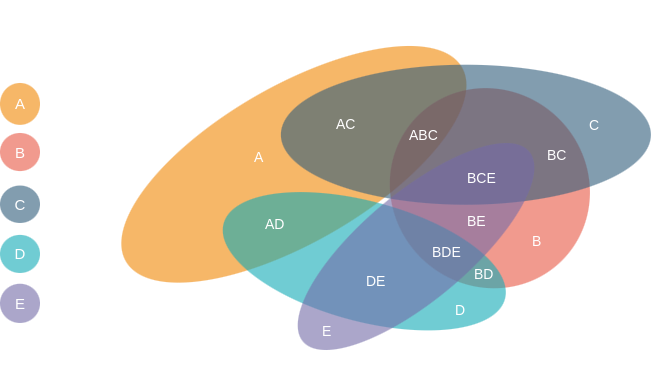
\includegraphics[scale=.35]{res/Not_Venn}
		\captionof{figure}{}\label{fig:notvenn}
	\end{minipage}
	\hfill
	\begin{minipage}{.45\textwidth}
		\centering
		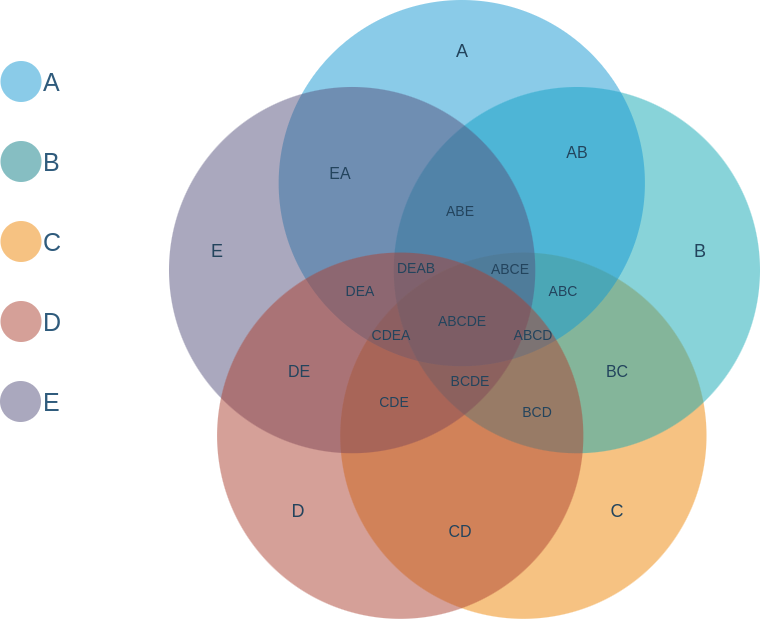
\includegraphics[scale=.25]{res/Venn}
		\captionof{figure}{}\label{fig:venn}
	\end{minipage}
\end{center}

\subsection{Le leggi di De Morgan e differenza simmetrica}
\begin{teorbox}
	Siano $a$, $b$, $c$ insiemi. Valgono allora le seguenti formule che prendono il nome di \textbf{leggi di De Morgan}:
	\begin{eqnarray}
		a \setminus (b \cap c) = (a \setminus b ) \cup (a \setminus c) \\
		a \setminus (b \cup c) = (a \setminus b) \cap (a \setminus c) \label{eq:demorgan2}
	\end{eqnarray}
\end{teorbox}

\begin{proof}
	Siano $\alpha,\beta,\gamma$ i predicati di appartenenza nella variabile $x$, rispettivamente: $\alpha$ è ``$x \in a$", $\beta$ è ``$x \in b$", $\gamma$ è ``$x \in c$". Da queste definizioni segue:
	\begin{align*}
		x \in a \setminus (b \cap c) &\iff \alpha \land \bigl(\neg (\beta \land \gamma)\bigr)  \\
		&\iff  \Bigl(\alpha \land \bigl((\neg \beta) \lor (\neg \gamma)\bigr)\Bigr)  \\
		&\iff  \Bigl(\bigl(\alpha \land (\neg \beta)\bigr) \lor \bigl(\alpha \land (\neg \gamma)\bigr)\Bigr)  \\
		&\iff  x \in (a \setminus b) \cup (a \setminus c)
	\end{align*}
	
	Similmente si dimostra l'equazione \ref{eq:demorgan2}.
\end{proof}


\dfn{Differenza simmetrica}{
	Si definisce l'operazione insiemistica $\triangle$ di \textbf{differenza simmetrica} l'operazione corrispondente alla disgiunzione esclusiva. Si pone dunque, per ogni insieme $a$ e $b$:
	\begin{equation}
		a \triangle b := \{ x \; | \; (x \in a) \xor (x \in b) \}
	\end{equation}
}


La tautologia che abbiamo chiamato \textbf{esplicitazione di XOR} (Vedi Formula \ref{eq:exclusive-or-2}) implica facilmente:
\begin{equation}
	a \triangle b = (a \setminus b) \cup (b \setminus a) = (a \cup b) \setminus (b \cap a)
\end{equation}
mentre la commutatività e l'associatività di $\xor$ e la distributività di $\land$ rispetto a $\xor$ forniscono la commutatività e l'associatività di $\triangle$ e la distributività di $\cap$ rispetto a $\triangle$. Per ogni insieme $a,b,c$ abbiamo cioè:
\begin{eqnarray}
	a \triangle b &=& b \triangle a \\
	a \triangle(b \triangle c) &=& (a \triangle b) \triangle c \\
	a \cap ( a \triangle c) &=& (a \cap b) \triangle (a \cup c)
\end{eqnarray}
\begin{center}
	% Definition of circles
	\def\firstcircle{(0,0) circle (1.5cm)}
	\def\secondcircle{(0:2cm) circle (1.5cm)}
	\colorlet{circle edge}{blue!50}
	\colorlet{circle area}{blue!20}
	\tikzset{filled/.style={fill=circle area, draw=circle edge, thick},
		outline/.style={draw=circle edge, thick}}
	\setlength{\parskip}{5mm}
	\begin{tikzpicture}
		\draw[filled, even odd rule] \firstcircle node {$a$}
		\secondcircle node{$b$};
	\end{tikzpicture}
	\captionof{figure}{$a \triangle b$}
\end{center}
\subsection{Operazioni unarie}
Per ogni insieme $s$ abbiamo definito l'insieme delle parti come l'insieme di tutti i sottoinsiemi di $s$. Dato però un numero naturale $n$ è possibile definire un altro insieme delle parti che va sotto il nome di \textbf{insieme delle parti $n$-arie}.

\dfn{Insieme delle parti $n$-arie}{
	Per ogni numero naturale $n \in \mathbb{N}$ e per ogni insieme $s$ si ha:
	\begin{equation}
		\mathcal{P}_{n}(s) = \biggl\{x \; | \; x \subseteq s \wedge \mbox{$x$  ha esattamente $n$ elementi}\biggr\}
	\end{equation}
}

\begin{example}
	Dato un insieme $s$ si ha $\mathcal{P}_{0}(s)= \{ \varnothing \} $ e $\mathcal{P}_{1}(s)= \bigl\{ \{x\} \; | \; x \in s \bigr\}$.
\end{example}

\dfn{Unione unaria}{
	Sia $a$ un insieme. Si definisce \textbf{unione unaria} di $a$ e si denota col simbolo $\bigcup a$ l'insieme:
	\begin{equation}
		\bigcup a = \{ x \; | \; \exists y \in a (x \in y)\}
	\end{equation}
	ovvero l'\textit{insieme degli elementi dei sottoinsiemi di $a$}.
}

\begin{example}
\begin{enumerate}
	\item Per ogni $m \in \mathbb{N}$ si pone:
\begin{displaymath}
	I_{m} = [0,m] = \{ x \in \mathbb{R} \; | \; 0 \leq x \leq m \}
\end{displaymath}
per definire un \textbf{intervallo chiuso reale} di estremi $0$ ed $m$. Denotiamo con $a= \{I_{m} \; | \; m \in \mathbb{N} \}$ l'insieme di tutti gli intervalli siffatti. Allora l'unione unaria di $a$ sarà:
\begin{displaymath}
	\bigcup a = \{x \in \mathbb{R} | x \geq 0 \} = \mathbb{R}^{+}
\end{displaymath}
\item Sia $S = \{\{1,5,7\},\{1,5,8,9\},\{2,15,66\}\}$, allora è:
\begin{displaymath}
	\bigcup S = \{1,2,5,7,8,9,15,66\}
\end{displaymath}
\end{enumerate}
\end{example}


\begin{example}
	L'unione unaria delle parti di $\mathbb{N}$ è $\mathbb{N}$ stesso. Infatti, preso un qualsiasi numero naturale è possibile prendere un sottoinsieme che lo contiene:
	\begin{displaymath}
		\forall n \in \mathbb{N} \bigl(\exists b \in \mathcal{P}(\mathbb{N})(n \in b)\bigr)
	\end{displaymath}
	Questo vuol dire allora che $\mathbb{N}$ è un sottoinsieme dell'unione unaria dell'insieme delle sue parti: $$\mathbb{N} \subseteq \bigcup \mathcal{P}(\mathbb{N})$$
	
	Per la definizione di inclusione (Formula \ref{eq:inclusione}) questo vuol dire che:
	\begin{displaymath}
		\forall x \bigl( x \in \mathbb{N} \implies x \in \bigcup \mathcal{P}(\mathbb{N}) \bigr)
	\end{displaymath}
	Preso un numero $y \notin \mathbb{N}$ ci chiediamo se questo possa appartenere a $\bigcup \mathcal{P} (\mathbb{N})$. Per appartenere a tale insieme deve soddisfare alla condizione:
	\begin{displaymath}
		y \in \bigcup \mathbb{N} \iff (\exists b \in \mathcal{P}(\mathbb{N})(y \in b))
	\end{displaymath}
	Il che è chiaramente falso in quanto abbiamo ipotizzato che $y$ non sia un numero naturale. Quindi possiamo dire che $\forall x \bigl( x \notin \mathbb{N} \implies x \notin \bigcup \mathcal{P}(\mathbb{N}) \bigr)$. Dalla \hyperlink{contrapposizione}{legge di contrapposizione} si ha quindi:$$\forall x (x \in \bigcup \mathcal{P}(\mathbb{N}) \implies x \in \mathbb{N})$$ Ovvero $\bigcup \mathcal{P}(\mathbb{N}) \subseteq \mathbb{N}$. e allora $\mathbb{N} = \bigcup \mathcal{P}( \mathbb{N})$ per la legge della doppia inclusione (Formula \ref{eq:doppia_inclusione}).
\end{example}

\dfn{Intersezione unaria}{
	Sia $a \neq \varnothing$ un insieme non vuoto. Si definisce \textbf{intersezione unaria} di $a$ e si denota col simbolo $\bigcap a$ l'insieme:
	\begin{equation}
		\bigcap a = \{x \; | \; \forall b \in a (x\in b)\}
	\end{equation}
	ovvero l'\textit{insieme degli elementi che appartengono a ciascun elemento di $a$}.
}


\begin{osservation}
\begin{enumerate}
	\item È importante precisare che $a$ non possa essere l'insieme vuoto altrimenti si avrebbe una contraddizione. Infatti:
	\begin{displaymath}
		\bigcap \varnothing = \{x | \forall y \in \varnothing (x \in y)\}
	\end{displaymath}
	il che rappresenterebbe l'insieme di tutti gli insiemi.
	
	\item Sia $c=\{a,b\}$ un insieme contenente gli insiemi $a$ e $b$. Quindi, per definizione di unione unaria si ha che $\bigcup c$ è l'insieme degli elementi che si trovano o in $a$ o in $b$:
	\begin{displaymath}
		\bigcup c = \{x \; | \; \exists y \in c (x \in y)\} = \{x \; | \; x \in a \vee x \in b\} = a \cup b
	\end{displaymath}
	Quindi l'unione tra due insiemi altro non è che un caso particolare dell'unione unaria applicato ad un insieme formato da due elementi. Grazie all'operazione unaria è possibile quindi effettuare unioni tra infiniti oggetti. Analogamente per l'intersezione unaria $\bigcap \{a,b\} = a \cap b$.
\end{enumerate}
\end{osservation}

\begin{propbox}[Formule generalizzate di associatività, distributività e di De Morgan]
	Per ogni $a,b$ insiemi non vuoti valgono:
	\begin{eqnarray}
		(\bigcap a) \cap (\bigcap b) = \bigcap (a \cup b) \\
		(\bigcap a) \cup (\bigcap b) = \bigcup (a \cap b )\\
		a \cap (\bigcup b) = \bigcup_{x \in b} (a \cap x) \\
		a \cup (\bigcap b) = \bigcap_{x \in b} (a \cup x)\\
		a \setminus \bigcup b = \bigcap_{x \in b} ( a \setminus x) \\
		a \setminus \bigcap b = \bigcup_{x \in b} (a \setminus x)
	\end{eqnarray}
\end{propbox}

\begin{proof} 
	La dimostrazione di queste formule è lasciata al lettore come esercizio.
\end{proof}

\section{Prodotto Cartesiano di Insiemi}

\subsection{Coppie ordinate}

\dfn{Coppia ordinata}{\index{Coppia ordinata}
	Siano $a$, $b$ insiemi. Una \textbf{coppia ordinata} si denota col simbolo $(a,b)$ e gode della seguente proprietà:
	\begin{equation}
		\forall \ a,b,c,d \qquad (a,b)=(c,d) \Longleftrightarrow (a=c \wedge b=d)
	\end{equation}
}

\begin{propbox}
	Per ogni $a,b,c,d$ si ha:
	\begin{displaymath}
		\{\{a\}, \{a,b\}\} = \{\{c\}, \{c,d\}\} \iff a = c \wedge b = d
	\end{displaymath}
\end{propbox}

\begin{proof}
	($\implies$) Si supponga quindi che $\{\{a\}, \{a,b\}\} = \{\{c\}, \{c,d\}\}$. Per l'assioma di estensionalità (Assioma \ref{axiom:extensionality}) allora entrambi gli insiemi hanno gli stessi elementi. Se $a=b$ allora $\{\{a\},\{a,b\}\}=\{\{a\}\}$ ha un solo elemento, per cui anche $\{\{c\},\{c,d\}\}$ ha un solo elemento. Quindi $a=b=c=d$.
	
	Sia allora $a \neq b$. Dall'ipotesi $\{\{a\}, \{a,b\}\} = \{\{c\}, \{c,d\}\}$ segue allora $c \neq d$, per cui deve essere:
	\begin{eqnarray*}
		\{a\}=\{c\} &\implies& a=c \\
		\{a,b\}=\{c,d\} &\implies& b=d
	\end{eqnarray*}
	
	($\impliedby$) Chiaramente la condizione è sufficiente.
\end{proof}

Si può usare questa proposizione per dare una definizione esplicita delle coppie ordinate, ponendo: $$\forall a,b \qquad (a,b) \coloneqq \{\{a\}, \{a,b\}\}$$  Questa è la cosiddetta \textbf{definizione di Kuratowski} della nozione di coppia ordinata.

\subsection{Prodotti cartesiani}

\dfn{Prodotto cartesiano}{\index{Prodotto cartesiano}
	Siano $a$, $b$ insiemi. Si dice \textbf{prodotto cartesiano} di $a$ e $b$, e si denota col simbolo $a \times b$, l'insieme di tutte le coppie $(x,y)$, con $x$ appartenente ad $a$ e $y$ appartenente a $b$.
	\begin{equation}
		a \times b = \bigl \{(x,y) \; | \; x \in a \wedge y \in b \bigl \}
	\end{equation}
}


\begin{example}
	Ad esempio se $a=\{1,2,3\}$ e $b=\{1,2\}$, allora $$a \times b=\{(1,1),(2,1),(3,1),(1,2),(2,2),(3,2)\}$$
	\begin{center}
		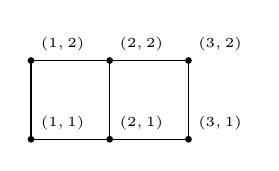
\begin{tikzpicture}
			\draw[step=1.0,black,thin] (1,1) grid (3,2);
			\foreach \x in {1,...,3}
			\foreach \y in {1,2}
			\filldraw (\x,\y) circle[radius=1pt] node[above right] {\tiny $(\x,\y)$};
		\end{tikzpicture}
	\end{center}
\end{example}

\dfn{Terna ordinata}{\index{Terna ordinata}
	Si definisce una \textbf{terna ordinata} $(a,b,c)$ come una coppia ordinata in cui la prima coordinata è una coppia ordinata $(a,b)$ e come seconda coordinata $c$:
	\begin{equation}
		\forall a,b,c \qquad (a,b,c) = \bigl((a,b),c\bigr)
	\end{equation}
}

\begin{propbox}\label{prop_terne_ordinate}
	Due terne ordinate $(a,b,c)$ e $(d,e,f)$ sono uguali se e solo se:
	\begin{equation}
		\forall a,b,c,d,e,f \qquad \bigl((a,b),c\bigr) = \bigl((d,e),f\bigr) \iff (a=d \wedge b=e \wedge c=f)
	\end{equation}
\end{propbox}

\begin{proof}
	L'enunciato si dimostra facilmente ponendo $(a,b)=m$ e $(d,e)=n$. In questo modo la dimostrazione si riduce alla dimostrazione già vista delle coppie ordinate $(m,c)$ e $(n,f)$. 
\end{proof}
\newpage
\section{Esercizi svolti}
\begin{exsbox}
	Verificare $3 \in \{2n^{2}+1 \; | \; n \in \mathbb{Z}\}$.
\end{exsbox}
\paragraph{Svolgimento.} Poniamo $A=\{2n^{2}+1 / n \in \mathbb{Z}\}$. Per essere verificata l'appartenenza deve valere la seguente equivalenza logica
\begin{displaymath}
	3 \in A \iff \exists n \in \mathbb{Z}(3=2n^{2}+1)
\end{displaymath}
e procediamo sviluppando algebricamente tale relazione fino ad ottenere una relazione più semplice da valutare:
\begin{align*}
	3 \in A &\iff \exists n \in \mathbb{Z}(3=2n^{2}+1)\\
	&\iff \exists n \in \mathbb{Z}(2=2n^{2}) & \text{\textcolor{gray}{Spostando 1 a sinistra}}\\
	&\iff \exists n \in \mathbb{Z}(n^{2}=1) & \text{\textcolor{gray}{Semplificando}}
\end{align*}
L'ultima equivalenza è chiaramente vera in quanto, per $n=\pm 1 \in \mathbb{Z}$ si ha $n^{2}=1$. Quindi $3 \in A$. \hfill \blacksquare
\begin{exsbox}
	Sia $A= \{\{a,b\}/a,b \in \mathbb{Z}\}$ un insieme. Verificare $\{1\} \in A$ e $\{1,2,3\} \in A$.
\end{exsbox}
\paragraph{Svolgimento.} Chiaramente:
\begin{align*}
	\{1\} \in A \iff \exists a,b \in \mathbb{Z}(\{a,b\} = \{1\})
\end{align*}
che risulta vera per $a=b=1$. Infatti $\{1,1\}=\{1\} \in A$. Al contrario, non esistono due numeri interi relativi tali che $\{a,b\}=\{1,2,3\}$ in quanto tale insieme contiene 3 elementi mentre $\{a,b\}$ ne può contenere al massimo due (quando $a \neq b$). Quindi $\{1,2,3\} \notin A$. \hfill \blacksquare
\begin{exsbox}
	Sia $f=\{\{a,b\},\{b,d\}\}$. Si calcolino $\bigcap f$ e $\bigcup f$.
\end{exsbox}
\paragraph{Svolgimento.} L'intersezione unaria di $f$ è definita come l'insieme degli elementi appartenenti a ciascun elemento di $f$, ovvero:
\begin{displaymath}
	\bigcap f = \{x / \forall y \in f (x \in y)\} = \{a,b\} \cap \{b,d\}= \{b\}
\end{displaymath}
\marker{yellow!50}{yellow!20!black}{Non dimenticare che $b \neq \{b\}$, nel primo caso ci si sta riferendo all'entità $b$ mentre nel secondo al singleton dell'entità $b$. \emph{Sarebbe stato un errore} scrivere quindi $\bigcap f = b$.}
Nel caso dell'unione unaria abbiamo che:
\begin{displaymath}
	\bigcup f = \{x / \exists y \in f (x \in f)\} = \{a,b\} \cup \{b,d\} = \{a,b,d\}
\end{displaymath}
\hfill \blacksquare
\begin{exsbox}
	Sia $A$ l'insieme dei numeri pari e $B$ quello dei numeri naturali moltiplicati per 2; dire in quale relazione stanno i due insiemi.
\end{exsbox}
\paragraph*{Svolgimento.} Per definizione di numero pari esprimiamo l'insieme $A$ come: $$\{p \in \mathbb{Z} / \exists k \in \mathbb{Z}(p = 2k)\}$$ mentre $$B= \{m \in \mathbb{N} / \exists k \in \mathbb{N} (m = 2k) \}$$ Ovviamente vale $B \subset A$. \hfill \blacksquare
\begin{exsbox}
	Decidere se esistono e, nel caso, descrivere esplicitamente gli insiemi:
	\begin{enumerate}
		\item $\{x | \forall y(x=y) \} $
		\item $\{ x|\forall y(x \neq y) \}$
		\item $ \{ x| \exists y (x=y)\}$
		\item $\{x|\exists y(x \neq y)\}$
		\item $ \{ x| \forall y (y \subseteq x) \}$
		\item $\{x|x=\{0,1,2\} \}$
		\item $\{y|y=\{0,1,2\} \}$
		\item $\{ x | x= \{0,1,2,x \} \}$
	\end{enumerate}
\end{exsbox}
\paragraph*{Svolgimento.} Si ha:
\begin{enumerate}
	\item  $\{x | \forall y(x=y) \} = \varnothing$. Non esiste infatti un insieme $x$ che sia uguale a tutti gli insiemi $y$. Quindi non esiste nessun elemento in questo insieme. Quindi l'insieme è l'insieme vuoto.
	\item $\{x|\forall y(x \neq y)\}= \varnothing$. Infatti non è vero che per ogni $x$, comunque si prenda un insieme $y$ allora $x \neq y$ perché appunto si potrebbe scegliere $x$ stesso al posto di $y$ ottenendo la proposizione ``$\forall x(x \neq x)$'' e poiché ogni oggetto è uguale a stesso allora si può dire che non esistono oggetti che appartengono alla totalità descritta dalla formula e per questo motivo l'insieme descrive l'insieme vuoto.
	\item Va notato che la proprietà di questo insieme è la negazione dell'insieme precedente. Per questo motivo possiamo dire che la proprietà è vera in quanto è vero che esiste almeno un insieme tale per cui sia uguale ad $x$ (ovvero $x$ stesso). Essendo vera questa formula allora sarebbe vero che per ogni insieme $x$ questo appartiene all'insieme $A=\{x|\exists y(x=y)\}$ ma non esistendo l'insieme di tutti gli insiemi allora l'insieme in questione non esiste.
	\item Analogamente come nell'esercizio precedente.
	\item L'insieme $\{x|\forall y(y \subseteq x)\}$ rappresenta l'insieme vuoto. Infatti non esiste un insieme tale per cui, comunque si scelga un insieme $y$, esso sia parte di $x$. Per fugare ogni dubbio, per rendere evidente che questa proposizione è false basta trovare un controesempio: preso l'insieme $x$ è immediato osservare che il singleton $\{x\}$ non è contenuto in $x$:$\forall x \bigl(\{x\} \nsubseteq x \bigr)$.
	\item L'insieme $\{x|x=\{0,1,2\}\}$ esiste ed ha un solo elemento. Infatti, per l'assioma di estensionalità, l'insieme delle $x$ tali che $x=\{0,1,2\}$ è il singleton di siffatto insieme $x$. Quindi:
	\begin{displaymath}
		\{x|x=\{0,1,2\}\} = \bigl\{ \{0,1,2\}  \bigr\}
	\end{displaymath}
	\item Uguale all'insieme precedente.
	\item $A=\{x|x=\{0,1,2,x\}\}=\varnothing$. Infatti si deve avere $\forall x(x \in A \iff \varphi)$, dove $\varphi$ rappresenta il predicato ``$x=\{0,1,2,x\}$''. Questa condizione è falsa per ogni $x$ in quanto nessun insieme appartiene a sé stesso e quindi l'insieme $A$ è vuoto. \hfill \blacksquare
\end{enumerate}
\begin{exsbox}
	Dire quali delle seguenti relazioni sono vere e quali false:
	\begin{enumerate}
		\item $\{1,3,5,10\} = \{3,1,10,5\}$;
		\item $\{a,b,d\}=\{b,d,a\}$;
		\item $\{2,5,6\} = \{2,7,5\}$;
		\item $\{a\} = a$;
		\item $a \in \{a\}$;
	\end{enumerate}
\end{exsbox}
\paragraph{Svolgimento.} Si ha:
\begin{enumerate}
	\item Vero
	\item Vero
	\item Falso
	\item Falso
	\item Vero \hfill \blacksquare
\end{enumerate}
\begin{exsbox}
	Sia $x=\{\{\{\{\varnothing\}\}\}\}$. Quanti elementi ha $x$? Quante parti ha $x$?
\end{exsbox}
\paragraph{Svolgimento.} L'insieme $x$ ha un solo elemento, di conseguenza l'insieme delle parti avrà solo le parti banali. \hfill \blacksquare
\begin{exsbox}
	Vero o falso?
	\begin{enumerate}
		\item $\varnothing \in \varnothing$
		\item $\varnothing \subseteq \varnothing$
		\item $\varnothing \subset \varnothing$
		\item $\varnothing \in \mathcal{P}(\varnothing)$
		\item $\varnothing \subseteq \mathcal{P}(\varnothing)$
		\item $\varnothing = \{\varnothing\}$
		\item $\varnothing \subseteq \{\varnothing\}$
		\item $\varnothing \in \{\varnothing\}$
		\item $\{1,1,2,2,2,3,3\}$ è una parte di $\{2,1,3\}$
		\item $\{1,1,2,2,2,3,3\}$ è una parte di $\{4,2,1,3\}$
	\end{enumerate}
\end{exsbox}
\paragraph{Svolgimento.} Si ha:
\begin{enumerate}
	\item Falso
	\item Vero
	\item Falso
	\item Vero
	\item Vero
	\item Falso
	\item Vero
	\item Vero
	\item Vero
	\item Vero. \hfill \blacksquare
\end{enumerate}
\begin{exsbox}
	Elencare gli elementi di $\mathcal{P}(\{0,1,2\})$.
\end{exsbox}
\paragraph{Svolgimento.}
Si ha $\mathcal{P}(\{0,1,2\})=\bigl\{ \varnothing, \{0,1,2\},\{ 0\},\{1\},\{2\},\{1,2\},\{0,1\},\{0,2\}   \bigr\} $.
\hfill \blacksquare

\begin{exsbox}
	Illustrare con i grafici di Eulero Venn la proprietà transitiva dell'inclusione tra i seguenti insiemi:
	\begin{displaymath}
		\begin{array}{lll}
			A = \{2,3,5\} & B= \{2,3,8,5\} & C = \{3,2,8,5,10,12\}
		\end{array}
	\end{displaymath}
\end{exsbox}
\paragraph{Svolgimento.} Si ha:
\begin{center}
	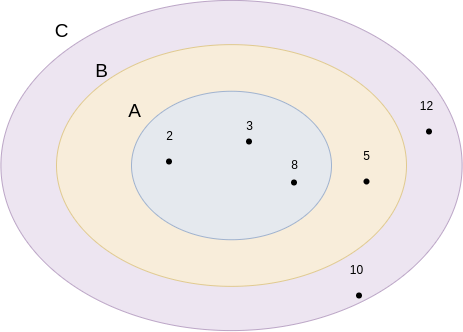
\includegraphics[scale=.45]{res/Venn_Esercizio1}
\end{center}
\hfill \blacksquare
\begin{exsbox}
	Determinare rispetto a $\mathbb{Z}$ gli insiemi complementari dei seguenti insiemi:
	\begin{enumerate}
		\item $\{x / x \in \mathbb{Z} \land x <3\}$
		\item $\{x / x \in \mathbb{Z} \land 2 \leq x \leq 5 \}$
		\item $\{x / x \in \mathbb{Z} \land 1 < x < 5 \}$
		\item $\{x / x \in \mathbb{Z} \land 1 \leq x \leq 2 \}$
		\item $\{x / x \in \mathbb{Z} \land x \geq 1 \}$
		\item $\{x / x \in \mathbb{Z} \land x \leq 0 \}$
	\end{enumerate}
\end{exsbox}
\paragraph{Svolgimento.} Definiamo complemento di una parte $X$ di un insieme non vuoto $S$ la differenza $S \setminus X$. Abbiamo allora:
\begin{enumerate}
	\item $\mathbb{Z} \setminus \{x / x \in \mathbb{Z} \land x <3\} = \{x / x \in \mathbb{Z} \land x > 3\}$;
	\item $\mathbb{Z} \setminus \{x / x \in \mathbb{Z} \land 2 \leq x \leq 5 \} = \{x / x \in \mathbb{Z} \land x < 2 \land x > 5\}$;
	\item $\mathbb{Z} \setminus \{x / x \in \mathbb{Z} \land 1 < x < 5 \} = \{x / x \in \mathbb{Z} \land x \leq 1 \land x \geq 5\}$;
	\item $\mathbb{Z} \setminus \{x / x \in \mathbb{Z} \land 1 \leq x \leq 2 \} = \{x /  x \in \mathbb{Z} \land x < 1 \land x > 2\}$;
	\item $\mathbb{Z} \setminus \{x / x \in \mathbb{Z} \land x \geq 1 \} = \{x / x \in \mathbb{Z} \land x < 1 \}$;
	\item $\mathbb{Z} \setminus \{x / x \in \mathbb{Z} \land x \leq 0 \} = \{x / x \in \mathbb{Z} \land x > 0 \}$. \hfill \blacksquare
\end{enumerate}
\begin{exsbox}
	L'insieme $\mathbb{Z}$ appartiene a $\mathcal{P}(\mathbb{Z})$?
\end{exsbox}
\paragraph{Svolgimento.} Sì. In ogni insieme $S \neq \emptyset$ si ha che $\emptyset$ ed $S$ sono parti banali e appartengono a $\mathcal{P}(S)$. \hfill \blacksquare
\begin{exsbox}
	Descrivere esplicitamente gli insiemi:
	\begin{enumerate}
		\item $\{x | \forall y (x \cap y = \varnothing)\}$
		\item $\{x | \exists y (x \cup y = \varnothing)\}$
		\item $\{x | \forall y (x \cup y = \varnothing)\}$
	\end{enumerate}
\end{exsbox}
\paragraph{Svolgimento.} Si ha:
\begin{enumerate}
	\item $\{x | \forall y (x \cap y = \varnothing)\}=\{ \varnothing \}$. Infatti l'insieme rappresenta l'insieme degli insiemi che non hanno alcun elemento in comune con tutti gli insiemi. L'unico insieme a soddisfare questa proprietà è l'insieme vuoto.
	\item $\{x | \exists y (x \cup y = \varnothing)\} = \{ \varnothing\}$. Infatti l'insieme rappresenta l'insieme di tutti gli insiemi $x$ per i quali esiste almeno un insieme $y$ tale che l'unione con $x$ sia il vuoto. L'unico insieme a soddisfare tale proprietà è l'insieme vuoto in quanto $\varnothing \cup \varnothing = \varnothing$.
	\item $\{x | \forall y (x \cup y = \varnothing)\}= \varnothing$. Infatti non esiste un insieme per cui la sua unione con qualsiasi insieme sia uguale all'insieme vuoto. \hfill \blacksquare
\end{enumerate}
\begin{exsbox}
	Per quali coppie di insiemi $a$, $b$, si ha $a \setminus b = b \setminus a$?
\end{exsbox}
\paragraph{Svolgimento.} L'unico caso in cui $a \setminus b$ può essere uguale a $b \setminus a$ è quando $a=b$. Infatti si ha $a \setminus b = \varnothing = b \setminus a$. \hfill \blacksquare
\begin{exsbox}
	Rappresentare, in diagrammi di Venn generici, i termini insiemistici $a \setminus ( b \setminus c)$ e $(a \setminus b) \setminus c$. Decidere se è vera o falsa la proposizione: $(\forall a,b,c)(a \setminus(b \setminus c) = (a \setminus b) \setminus c)$. Ripetere l'esercizio per $a \cap (b \setminus c)$ e $(a \cap b)\setminus c$.
\end{exsbox}
\paragraph{Svolgimento.}
L'insieme $a\setminus(b\setminus c)$ è rappresentato dal diagramma di Venn \ref{fig:venn228} mentre l'insieme $(a\setminus b)\setminus c$ dal diagramma \ref{fig:venn2282}.
\begin{center}
	\begin{minipage}{.45\textwidth}
		\centering
		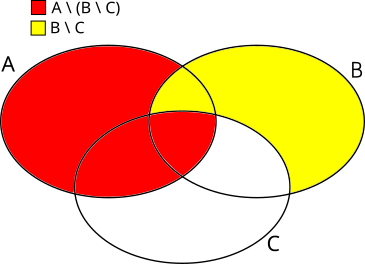
\includegraphics[scale=0.6]{res/path33251.png}
		\captionof{figure}{}\label{fig:venn228}
	\end{minipage}
	\hfil
	\begin{minipage}{.45\textwidth}
		\centering
		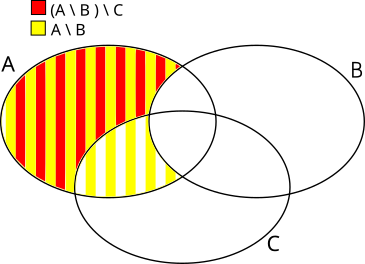
\includegraphics[scale=0.6]{res/path2879.png}
		\captionof{figure}{}\label{fig:venn2282}
	\end{minipage}
\end{center}
Osservando i due diagrammi possiamo concludere che la differenza simmetrica tra tre insiemi non gode della proprietà associativa. Non è vero dunque che:
$\forall \ a,b,c \Bigl(a \setminus (b\setminus c) = (a \setminus b) \setminus c \Bigr)$. Analogamente, i diagrammi di Eulero Venn \ref{fig:venn2283} e \ref{fig:venn2284} rappresentano gli insiemi $a\cap(b \setminus c)$ e $(a \cap b) \setminus c$.
\begin{center}
	\begin{minipage}{.45\textwidth}
		\centering
		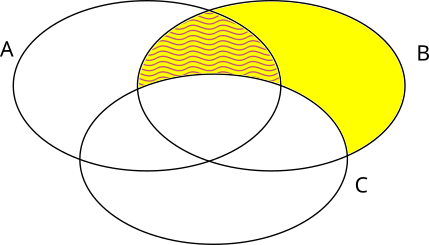
\includegraphics[scale=0.5]{res/Venn2882.png}
		\captionof{figure}{}\label{fig:venn2283}
	\end{minipage}
	\hfil
	\begin{minipage}{.45\textwidth}
		\centering
		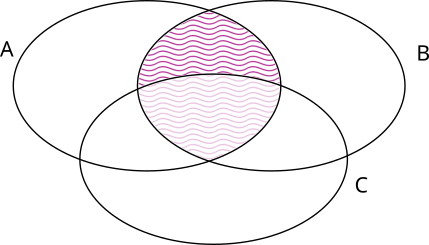
\includegraphics[scale=0.5]{res/Venn2882_2.png}
		\captionof{figure}{}\label{fig:venn2284}
	\end{minipage}
\end{center}
Dai due diagrammi ci si può convincere del fatto che: $\forall \ a,b,c \Bigl(a\cap(b \setminus c) = (a \cap b) \setminus c \Bigr)$. \hfill \blacksquare
\begin{exsbox}
	Rappresentare in diagramma di Eulero Venn $(a \triangle b) \triangle c$.
\end{exsbox}
\paragraph*{Svolgimento.}
Si ha che $(a \setminus b)\setminus c$ è uguale al seguente diagramma di Eulero Venn:
\begin{center}
	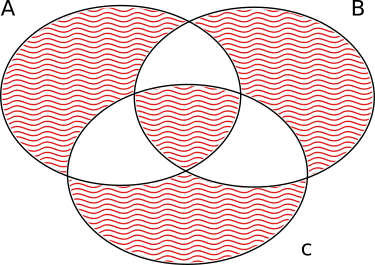
\includegraphics[scale=0.6]{res/diff3sim.png}
\end{center}

Infatti, posto $\alpha= x \in A$, $\beta=x \in B$ e $\gamma=x\in C$ si ha:
\begin{displaymath}
	x \in	(a \triangle b)\triangle c \iff \bigl( \alpha \xor \beta \bigr) \xor \gamma
\end{displaymath}
Che, per la tautologia \ref{eq:xor2} è equivalente all'implicazione:
\begin{displaymath}
	(\alpha \iff \beta) \iff \gamma
\end{displaymath}
che è vera quando vale una e una sola delle tre proprietà (come evidenziato dalle zone in verde alle estremità del diagramma) oppure valgono contemporaneamente (la parte centrale del diagramma).  \hfill \blacksquare

\begin{exsbox}
	Dimostrare che, per ogni $a$, $b$ sono equivalenti tra loro:
	\begin{enumerate}
		\item $a \subseteq b$
		\item $a \cap b = a$
		\item $a \cup b = b$
	\end{enumerate}
\end{exsbox}
\paragraph{Svolgimento.} ($1 \implies 2$) Dire che per ogni insieme $a$ e $b$ si ha $a \subseteq b$ significa affermare:
\begin{displaymath}
	\forall x (x \in a \implies x \in B)
\end{displaymath}
Poiché l'intersezione tra i due insiemi è l'insieme che contiene gli elementi in comune tra i due è evidente che l'insieme formato sia $a$.

($1 \implies 3$) Analogamente, se $a$ è un sottoinsieme di $b$ e l'unione è l'insieme formato da tutti gli elementi che si trovano o in $a$ o in $b$ allora l'unione tra i due insiemi è $b$ stesso.

($3 \implies 1$) Se $a \cup b = \{x | x \in a \lor x \in b\} = b$ può significare solo due cose. O che $a$ è l'insieme vuoto o che $a$ è un sottoinsieme di $b$. In entrambi i casi si ha $a \subseteq b$. \hfill \blacksquare

\begin{exsbox}
	Calcolare, per un arbitrario insieme $a$:
	\begin{enumerate}
		\item $a \triangle a$
		\item $a \triangle \emptyset $
	\end{enumerate}
\end{exsbox}
\paragraph{Svolgimento.} Per definizione di differenza simmetrica si ha:
\begin{align*}
	a \triangle a &= \{ x \; | \; x \in \bigl(( a \cup a) \setminus (a \cap a)\bigr) \}  \\
	&= \{x \; | \; x \in (a \setminus a) \} \\
	&= \varnothing
\end{align*}
mentre nel caso della seconda formula:
\begin{align*}
	a \triangle \varnothing &= \{ x \; | \; x \in \bigl(( a \cup \varnothing ) \setminus (a \cap \varnothing)\bigr) \} \\
	&= \{x \; | \; x \in (a \setminus \varnothing ) \} \\
	&= a
\end{align*}
\hfill \blacksquare

\begin{exsbox}
	Rappresentare, in un diagramma di Venn generico, il termine insiemistico $A \cap ( B \triangle C)$.
\end{exsbox}
\paragraph{Svolgimento. }Si procede calcolando innanzitutto $B \triangle C$ (la zona evidenziata di grigio) e poi si calcola l'intersezione con l'insieme $A$. Si ottiene così il diagramma di Venn mostrato in figura:
\begin{center}
	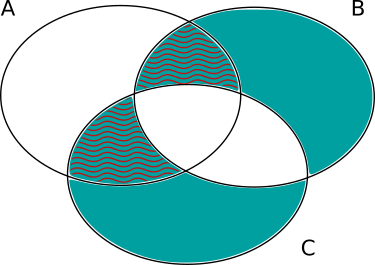
\includegraphics[scale=.6]{res/Venn_Esercizio2.png}
\end{center}
\hfill \blacksquare
\begin{exsbox}
	Rappresentare su un diagramma di Venn di tipo generale l'espressione insiemistica:
	$(A \setminus B) \triangle (B \cup C)$.
\end{exsbox}
\paragraph{Svolgimento.} Si ha:
\begin{align*}
	(A \setminus B) \triangle (B \cup C) &= \bigl((A \setminus B)  \cup (B \cup C)\bigr) \setminus \bigl((A \setminus B) \cap (B \cup C)\bigr) \\
\end{align*}
\begin{center}
	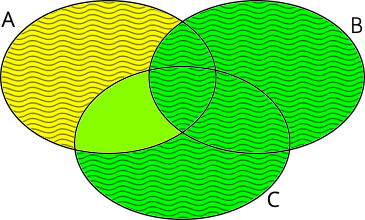
\includegraphics[scale=.6]{res/Venn_Esercizio3.png}
\end{center}
\hfill \blacksquare
\begin{exsbox}
	Rappresentare, in un diagramma di Venn generico, i termini insiemistici $A \cup (B \cap C)$ e $A \cap (B \cup C)$. Decidere se vale una delle formule:
	\begin{eqnarray}
		\forall A,B,C (A \cup (B \cap C) \subseteq A \cap (B \cup C))  \\
		\forall A,B,C (A \cup (B \cap C) \supseteq A \cap (B \cup C))
	\end{eqnarray}
\end{exsbox}
\paragraph{Svolgimento.}
Si ha $A \cup (B \cap C)$ rappresentato in figura \ref{fig:venn4} mentre $A \cap (B \cup C)$ è mostrato in Figura \ref{fig:venn5}.
\begin{center}
	\begin{minipage}{.45\textwidth}
		\centering
		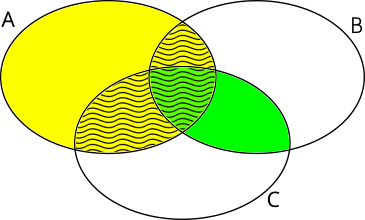
\includegraphics[scale=.6]{res/Venn_Esercizio4.png}
		\captionof{figure}{$A \cup (B \cap C)$}\label{fig:venn4}
	\end{minipage}
	\hfil
	\begin{minipage}{.45\textwidth}
		\centering
		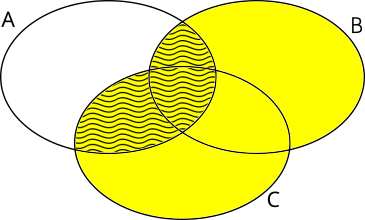
\includegraphics[scale=.6]{res/Venn_Esercizio5.png}
		\captionof{figure}{$A \cap (B \cup C)$}\label{fig:venn5}
	\end{minipage}
\end{center}
Osservando i diagrammi di Venn possiamo dire con certezza che $\forall A,B,C (A \cup (B \cap C) \supseteq A \cap (B \cup C))$. \hfill \blacksquare
\begin{exsbox}
	Rappresentare con un diagramma di Eulero Venn l'insieme: $\Bigl( \bigl(   (a \triangle b) \triangle c \bigr) \triangle d \Bigr)$.
\end{exsbox}
\paragraph{Svolgimento.} Affermare che un qualsiasi $x$ appartiene all'insieme $\Bigl( \bigl( (a \triangle b) \triangle c \bigr) \triangle d   \Bigr)$ è equivalente alla seguente catena di implicazioni:
\begin{align*}
	\forall x \biggl( x \in \Bigl( \bigl( (a \triangle b) \triangle c \bigr) \triangle d   \Bigr) \biggr) &\iff \forall x \Bigl( x \in \bigl( (a \triangle b) \triangle c \bigr) \xor (x \in d) \Bigr) \\
	&\iff \forall x \Bigl( \bigl( x \in (a \triangle b) \xor x \in c  \bigr) \xor (x \in d)        \Bigr) \\
	&\iff \forall x \Bigl( (x \in a) \xor (x \in b) \xor (x \in c) \xor (x \in d)   \Bigr)
\end{align*}
che è vera quando è vera singolarmente una delle condizioni di appartenenza oppure quando vale per tre di esse. Quindi l'insieme così ottenuto è quello evidenziato dalle strisce nel diagramma di Eulero Venn mostrato nella Figura \ref{fig:venn215}.
\begin{center}
	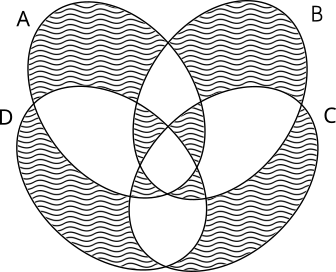
\includegraphics[scale=0.7]{res/path9768.png}
	\captionof{figure}{}\label{fig:venn215}
\end{center}
\begin{exsbox}
	Rappresentare, in diagrammi di Venn generici, i termini insiemistici $a \cap (b \triangle c)$ e $a \cup (b \triangle c)$, confrontandoli tra loro e con $(a \cap b) \triangle (a \cap c)$ e $(a \cup b) \triangle (a \cup c)$.
\end{exsbox}
\paragraph{Svolgimento.} Si ha:
\begin{center}
	\begin{minipage}{.45\textwidth}
		\centering
		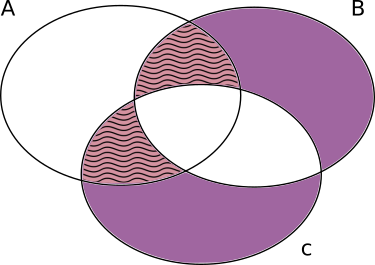
\includegraphics[scale=.5]{res/Venn_Esercizio6.png}
		\captionof{figure}{$a \cap (b \triangle c)$}
	\end{minipage}
	\begin{minipage}{.45\textwidth}
		\centering
		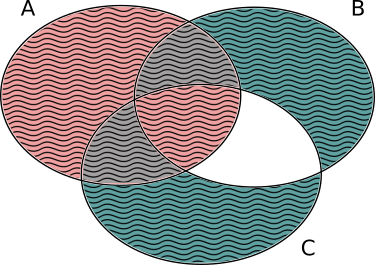
\includegraphics[scale=.5]{res/Venn_Esercizio7.png}
		\captionof{figure}{$a \cup (b \triangle c)$}
	\end{minipage} \\
	\begin{minipage}{.45\textwidth}
		\centering
		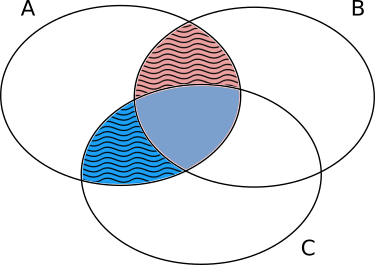
\includegraphics[scale=.5]{res/Venn_Esercizio8.png}
		\captionof{figure}{$(a \cap b) \triangle (a \cap c)$}
	\end{minipage}
	\begin{minipage}{.45\textwidth}
		\centering
		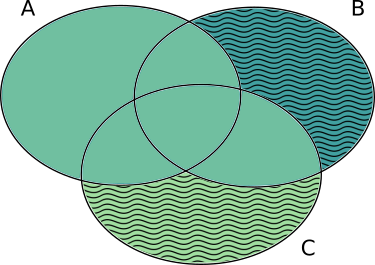
\includegraphics[scale=.5]{res/Venn_Esercizio9.png}
		\captionof{figure}{$(a \cup b) \triangle (a \cup c)$}
	\end{minipage}
\end{center}
Osservando i vari diagrammi di Venn possiamo dire con certezza che vale:
\begin{displaymath}
	\begin{array}{l}
		a \cap (b \triangle c) = (a \cap b) \triangle (a \cap c)  \\
		a \cap (b \triangle c) \subset a \cup (b \triangle c) \\
		(a \cup b) \triangle (a \cup c) \subset  a \cup (b \triangle c)
	\end{array}
\end{displaymath}
\hfill \blacksquare
\begin{exsbox}
	Siano $a$ e $b$ due insiemi. Supposto $a \subseteq b$, descrivere $a \triangle b$.
\end{exsbox}
\paragraph{Svolgimento.} Per definizione
\begin{equation}\label{eq:diff_simm_parti}
	a \triangle b = (a \cup b) \setminus (a \cap b)
\end{equation}
Ma, essendo $a \subseteq b$, valgono le seguenti relazioni:
\begin{eqnarray}
	a \cup b = b \\
	a \cap b = a
\end{eqnarray}
Quindi, sostituendo tali relazioni in \ref{eq:diff_simm_parti} si ottiene:
\begin{align*}
	a \triangle b &= (a \cup b) \setminus (a \cap b) \\
	&= b \setminus a
\end{align*}
Ovvero il complemento di $a$ in $b$ come mostrato nel seguente diagramma di Venn:
\begin{center}
	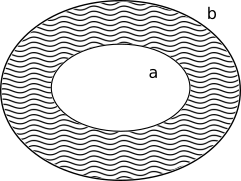
\includegraphics[scale=.8]{res/Venn_Esercizio10}
\end{center}
\hfill \blacksquare
\begin{exsbox}
	Siano $A=\{n \in \mathbb{N} \; | \; 3 \leq n \leq 10\}$, $B$ l'insieme dei numeri naturali pari, $C=\{1,2,8,13,1234\}$. Descrivere, elencandone gli elementi:
	\begin{enumerate}
		\item $A\setminus B$
		\item $A \triangle C$
		\item $B \cap C$
		\item $B \triangle (B \setminus C)$.
	\end{enumerate}
\end{exsbox}
\paragraph{Svolgimento.} Abbiamo:
\begin{displaymath}
	\begin{array}{l}
		A \setminus B = \{3,5,7,9\}\\
		A \triangle C = \{1,2,4,5,6,7,9,10,13,1234\}\\
		B \cap C = \{2,8,1234\}\\
		B \triangle (B \setminus C) = \{2,8,1234\}
	\end{array}
\end{displaymath}
\marker{yellow!50}{yellow!20!black}{Sfrutta la proprietà della differenza simmetrica tra un insieme ed una sua parte dimostrata nell'esercizio precedente.}
\hfill \blacksquare
\begin{exsbox}
	Calcolare:
	\begin{enumerate}
		\item $ \bigcup \varnothing$
		\item $ \bigcup \{ \varnothing \} $
		\item $ \bigcup \{ a \}$
		\item $ \bigcap \{ a \} $
	\end{enumerate}
\end{exsbox}
\paragraph{Svolgimento.} Si ha:
\begin{align*}
	\bigcup  \varnothing &= \varnothing \\
	\bigcup  \{ \varnothing \} &= \{ x \; | \; x \in \varnothing \} = \varnothing  \\
	\bigcup  \{a \} &= \{ x \; | \; x \in \{ a \} \} = a \\
	\bigcap  \{a \} &= a
\end{align*}
\hfill \blacksquare
\begin{exsbox}
	Calcolare $\bigcap A$ e $\bigcup A$ in ciascuno dei seguenti casi:
	\begin{enumerate}
		\item A è l'insieme delle parti infinite di $\mathbb{N}$
		\item $A=\{X \subseteq \mathbb{N} \;|\; 13 \notin X \}$
		\item $A=\{X \subseteq \mathbb{N} \;|\; 13 \in X \}$
		\item $A=\{\{124,n\} \; | \; n \in \mathbb{N}\}$
		\item $A=\{[n-1,n+1] \; | \; n \in \mathbb{N}\}$ dove $[a,b]=\{x \in \mathbb{R} \; | \; a \leq x \leq b \}$
	\end{enumerate}
\end{exsbox}
\paragraph{Svolgimento.} Si ha:
\begin{enumerate}
	\item $\bigcup A = \mathbb{N}$, $\bigcap A = \varnothing$. 	Se supponiamo infatti che esista un elemento $x$ appartenente a tutte le parti infinite di $\mathbb{N}$, cioè $\bigcap A = \{x\}$. Allora $x \in \mathbb{N}$ e vale $\forall x( x \notin \mathbb{N}\setminus\{x\})$, dove $\mathbb{N}\setminus\{x\}$ è una parte infinita di $\mathbb{N}$ e il che è assurdo.
	\item $\bigcup A = \mathbb{N}\setminus \{13\}$,	$\bigcap A = \varnothing$
	\item 	$\bigcup A = \mathbb{N}$, $\bigcap A = \{13\}$
	\item 	$\bigcup A = \mathbb{N}$, $\bigcap A = \{124\}$
	\item $\bigcup A = \{x \in \mathbb{R} \; | \; x \geq -1 \} $, $\bigcap A = \varnothing$
\end{enumerate}
\hfill \blacksquare
\begin{exsbox}
	Vero o falso?
	\begin{enumerate}
		\item $(\{0\} \times \mathbb{N}) \cap (\{1\} \times \mathbb{N}) = \{0,1\} \times \mathbb{N}$
		\item $(\mathbb{N} \times \mathbb{N}) \cup \bigl((\mathbb{Z}\setminus \mathbb{N})\times (\mathbb{Z} \setminus \mathbb{N})\bigr)= \mathbb{Z} \times \mathbb{Z}$
	\end{enumerate}
\end{exsbox}
\paragraph{Svolgimento.} 	Si ha:
\begin{enumerate}
	\item $(\{0\}\times \mathbb{N})\cap (\{1\}\times \mathbb{N}) \neq \{0,1\}\times \mathbb{N}$. Infatti $(\{0\}\times \mathbb{N})$ rappresenta l'insieme di tutte le coppie del tipo $(0,n)$ con $n \in \mathbb{N}$ mentre $(\{1\}\times \mathbb{N})$ quello delle coppie del tipo $(1,n)$ con $n \in \mathbb{N}$ quindi la loro intersezione è sicuramente vuota.
	\item $(\mathbb{N}\times \mathbb{N})\cup \bigl((\mathbb{Z} \setminus \mathbb{N}) \times (\mathbb{Z} \setminus \mathbb{N})\bigr) \neq \mathbb{Z} \times \mathbb{Z}$. Infatti:
	\begin{displaymath}
		(\mathbb{N}\times \mathbb{N})\cup \bigl((\mathbb{Z} \setminus \mathbb{N}) \times (\mathbb{Z} \setminus \mathbb{N})\bigr) =	\{(n,m)| n,m \in \mathbb{N}\} \cup \{(-n,-m) | n,m \in \mathbb{N} \}
	\end{displaymath}
	Preso un elemento di $\mathbb{Z} \times \mathbb{Z}$, ad esempio $(1,-2)$ si vede facilmente che questo non appartiene al primo insieme. \hfill \blacksquare
\end{enumerate}

\begin{exsbox}
	Verificare che:
	\begin{enumerate}
		\item $A \setminus B = A \implies A \cap B = \emptyset$
		\item $A \setminus B = \emptyset \implies A \subseteq B$
		\item $A \cap ( B \setminus C) = (A \cap B) \setminus (A \cap C)$
	\end{enumerate}
\end{exsbox}
\paragraph{Svolgimento.}
\begin{enumerate}
	\item Supponiamo che $A \cap B \neq \emptyset$. Allora, essendo non vuoto, esiste un elemento appartenente a tale intersezione, sia esso $\overline{x} \in A \cap B$. Per definizione di intersezione si ha:
	\begin{displaymath}
		\overline{x} \in A \cap B \iff x \in A \land x \in B
	\end{displaymath}
	Consideriamo adesso la differenza $A \setminus B$ definito come:
	\begin{displaymath}
		A \setminus B = \{x / x \in A \land x \notin B \}
	\end{displaymath}
	ovviamente si ha che $\overline{x} \notin A \setminus B$. Per questo e per la generalità di $\overline{x}$ possiamo affermare quindi che $A \cap B \nsubseteq A \setminus B$. Sapendo che l'intersezione tra due insiemi è sempre una parte di entrambi gli insiemi, affermare che $A \cap B \nsubseteq A \setminus B$ equivale a dire che $A \setminus B \neq A$ in quanto da tale insieme mancano sicuramente gli elementi appartenenti a $A \cap B$. Per contrapposizione si ha la tesi.
	\item Supponiamo che $A$ non sia una parte di $B$. Per definizione di sottoinsieme abbiamo che:
	\begin{align}
		A \subseteq B &\iff \forall x \in A (x \in B)
	\end{align}
	Allora, negando:
	\begin{align*}
		A \nsubseteq B &\iff \neg \bigl(\forall x (x \in A \implies x \in B)\bigr)\\
		&\iff \exists x ( x \in A \land x \notin B) & \text{\textcolor{gray}{Negando il quantificatore universale}} \\
		&\iff \exists x \in A \setminus B & \text{\textcolor{gray}{Per definizione di differenza}} \\
	\end{align*}
	Quindi $A \setminus B \neq \emptyset$. Per contrapposizione si ottiene la tesi.
	\item Dimostriamo innanzitutto che $A \cap (B \setminus C) \subseteq (A \cap B) \setminus (A \cap C)$. Sia $x \in A \cap (B \setminus C)$ allora $x$ appartiene sia ad $A$ che a $B \setminus C$, ovvero $x$ appartiene sia ad $A$ che a $B$ ma non appartiene a $C$. Pertanto $x$ appartiene a ciascuna delle differenze $A \setminus C$ che $B \setminus C$. Da $x \in A \setminus C$ possiamo osservare che sicuramente $x \notin A \cap C$ e vale quindi $x \in (A \cap B) \setminus (A \cap C)$, ovvero vale: $A \cap (B \setminus C) \subseteq (A \cap B) \setminus (A \cap C)$.
	
	Viceversa, se $x \in (A \cap B) \setminus (A \cap C)$, si ha che $x$ appartiene a $A \cap B$ e $x \notin (A \cap C)$ per cui $x$ non appartiene ad almeno uno degli insiemi $A$ e $C$. Se $x \in A \cap B$ sicuramente deve essere $x \notin C$ e allora si ha che $x \in A \land x \in B \land x \notin C$, per associatività quindi: $x \in A \cap (B \setminus C)$ e la tesi è dimostrata avendo ottenuto la doppia inclusione. \hfill \blacksquare
\end{enumerate}
\begin{exsbox}
	Si dimostri che se $B$ è un insieme e $A \subseteq B$ allora $(B \setminus A) \cap A = \emptyset $ e $(B \setminus A) \cup A = B$.
\end{exsbox}
\paragraph{Svolgimento.} Per dimostrare che un certo insieme è vuoto conviene ragionare per assurdo, cioè supporre che non sia vuoto e dedurne una contraddizione. Ad esempio, siano $A \subseteq B$ due insiemi e supponiamo per assurdo che $(B \setminus A) \cap A \neq \emptyset$. Da $(B \setminus A) \cap A \neq \emptyset$ segue che $\exists x \in (B \setminus A) \land x \in A$. Ne segue che $x \notin A$ e $x \in A$ e questa è una contraddizione. Abbiamo così dimostrato che deve essere $(B \setminus A) \cap A = \emptyset$.

Mostriamo ora che se $A \subseteq B$, allora $(B \setminus A) \cup A = B$. Dato che $B \setminus A \subseteq B$ e $A \subseteq B$, abbiamo che $(B \setminus A) \cup A  \subseteq B$. Per mostrare che $B \subseteq (B \setminus A) \cup A$ fissiamo $b \in B$. Allora si possono avere i due casi $b \in A$ oppure $b \notin A$. Se $b \in A$, allora $b \in (B \setminus A) \cup A$. Se invece $b \notin A$, si ha che $b \in B \setminus A$, e quindi $b \in (B \setminus A) \cup A$. In entrambi i casi si ha pertanto che $b \in (B \setminus A) \cup A$ e quiesto prova che $B \subseteq (B \setminus A) \cup A$. \hfill \blacksquare
\begin{exsbox}
	Siano $a$ e $b$ due insiemi. Si ha $a \times b = b \times a$ se e solo se ...?
\end{exsbox}
\paragraph{Svolgimento.} Dati due insiemi $a$ e $b$ si ha che $a \times b = b \times a $ se e solo se $a = b$. Essendo la condizione banalmente sufficiente\footnote{Si veda l'osservazione \ref{oss:condizionenecessariasufficiente}} dimostriamo che essa è necessaria, ovvero $a \times b = b \times a \implies a=b$. Prendiamo un qualsiasi elemento $x \in a$. Se $y \in b$ allora la coppia $(x,y)\in a \times b = b \times a$. Allora $x$ appartiene anche all'insieme $b$ e, per la sua generalità, possiamo dire che $a \subseteq b$. Analogamente per la seconda coordinata si ha che $y \in a$ e quindi $b \subseteq a$. Per la legge della doppia inclusione allora abbiamo $a=b$. \hfill \blacksquare
\begin{exsbox}
	Siano $A$ e $B$ due sottoinsiemi di $I$ e sia $B'$ il complementare di $B$ rispetto a $I$. Verificare che $A \setminus B = A \cap B'$.
\end{exsbox}
\paragraph*{Svolgimento.} Confrontando i due diagrammi di Venn si ha la verifica dell'asserto:
\begin{center}
	\begin{minipage}{.45\textwidth}
		\centering
		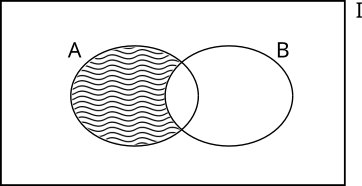
\includegraphics[scale=.6]{res/Venn_Esercizio11}
	\end{minipage}
	\hfil
	\begin{minipage}{.45\textwidth}
		\centering
		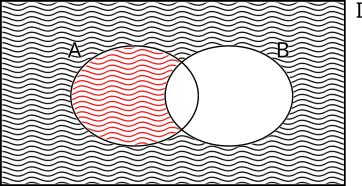
\includegraphics[scale=.6]{res/Venn_Esercizio12}
	\end{minipage}
\end{center}
Si può arrivare alla stessa conclusione osservando che un elemento $x$ appartiene all'insieme $A \setminus B$ se, e soltanto se, $x$ appartiene ad $A$ ma non appartiene a $B$. Sfruttando il fatto che $A$ è una parte di $I$ abbiamo sicuramente che $x$ è un elemento appartenente anche ad $I$, ovvero: $\forall x \in (A \setminus B) (x \in A \land x \in I \land x \notin B)$ il che è equivalente ad affermare che $x \in A \land x \in B'$ e quindi si ha che $A \setminus B \subseteq A \cap B'$. Viceversa, sia $x \in A \cap B'$. Si ha ovviamente che $x$ appartiene sia ad $A$ che al complemento di $B$, ovvero $I \setminus B$. Quindi $x \in A$, $x \in I$ e $x \notin B$. Allora $x$ appartiene ad $A$ e non appartiene a $B$, ovvero $x \in A \setminus B$ e vale $A \cap B' \subseteq A \setminus B$. Dalla doppia inclusione deriva l'asserto. \hfill \blacksquare

\begin{exsbox}
	Dimostrare che, per ogni insieme $A$, $B$:
	\begin{displaymath}
		A \times B = \varnothing \iff A = \varnothing \vee B = \varnothing
	\end{displaymath}
\end{exsbox}
\paragraph{Svolgimento}
\begin{itemize}
\item[$\impliedby$] La condizione è ovviamente sufficiente.	
\item[$\implies$] Ragionando per contrapposizione, si ottiene:
\begin{displaymath}
	\forall A,B (A = \varnothing \vee B = \varnothing)
\end{displaymath}
quindi:
\begin{displaymath}
	\exists A,B (A \neq \varnothing \wedge B \neq \varnothing)
\end{displaymath}
dunque:
\begin{displaymath}
	\exists a \in A \wedge \exists b \in B
\end{displaymath}
Fissati tali $a,b$ si ottiene:	$(a,b) \in A \times B \neq \varnothing$.\hfill \blacksquare
\end{itemize}
\begin{exsbox}
	Elencare gli elementi di $\{1,2 \} \times \{1,2,3\}$, quelli di $\{1,2,3 \} \times \{1,2\}$ e quelli di $( \{1,2\} \times \{1,2,3\} ) \cap ( \{1,2,3\} \times \{1,2\})$.
\end{exsbox}
\paragraph{Svolgimento.} Si ha:
\begin{itemize}
	\item $\{1,2 \} \times \{1,2,3\} = \{(1,1),(1,2),(1,3),(2,1),(2,2),(2,3)\}$
	\item $\{1,2,3 \} \times \{1,2\} = \{(1,1),(1,2),(2,1),(2,2),(3,1),(3,2)\}$
	\item $\{1,2\} \times \{1,2,3\} ) \cap ( \{1,2,3\} \times \{1,2\}) = \{(1,1),(1,2),(2,2)\}$. \hfill \blacksquare
\end{itemize}
\begin{exsbox}
	Vero o falso?
	\begin{enumerate}
		\item $(\{0\}\times \mathbb{N}) \cup (\{1\}\times \mathbb{N}) = \{0,1\} \times \mathbb{N}$
		\item $(\mathbb{N} \times \mathbb{N}) \cup (\mathbb{Z} \setminus \mathbb{N}) \times (\mathbb{Z}\setminus \mathbb{N}) = \mathbb{Z} \times \mathbb{Z}$.
	\end{enumerate}
\end{exsbox}
\paragraph{Svolgimento.} 
\begin{enumerate}
	\item Vero, perché $(\{0\}\times \mathbb{N}) \cup (\{1\}\times \mathbb{N})$ è l'unione  tra l'insieme di tutte le coppie di prima coordinata 0 e seconda coordinata un naturale e l'insieme di tutte le coppie di prima coordinata 1 e seconda coordinata un naturale.
	\item Vero, perché $\mathbb{Z} \times \mathbb{Z}$ può essere visto come l'unione tra l'insieme delle coppie $(a,b)$ con $a,b$ entrambi positivi e l'insieme delle coppie $(c,d)$ con $c,d$ entrambi negativi. \hfill \blacksquare
\end{enumerate}
\gbox{Tecniche di dimostrazione}{red}{
	Un \textbf{teorema} è un enunciato della forma ``Se valgono $P_{1},P_{2},\ldots,P_{n}$ allora vale anche $Q$'' che equivale alla formula logica: $P_{1} \land P_{2} \land \ldots \land P_{n} \implies Q$. Le affermazioni $P_{1},P_{2},\ldots,P_{n}$ sono dette \textbf{ipotesi} mentre $Q$ è la \textbf{tesi} del teorema. Come possiamo organizzare in modo rigoroso un ragionamento e stabilire che esso costituisce la dimostrazione di un teorema? Ci sono diverse strategie dimostrative variamente utilizzate:
	\begin{itemize}
		\item  la \textbf{dimostrazione diretta} è la strategia più semplice e naturale per stabilire un teorema del tipo descritto. La dimostrazione diretta assume di trovarsi in un qualunque contesto in cui siano verificate le ipotesi e sulla base di semplici e rigorosi ragionamenti stabilisce che in tale contesto anche la tesi è verificata.
		\item la \textbf{dimostrazione per assurdo} consiste in una dimostrazione in cui si assume che la tesi sia falsa e da questa assunzione si deriva (utilizzando anche le ipotesi) una contraddizione, ovvero una proposizione della forma $p \land (\neg p)$ che asserisce che una qualche affermazione $p$ è contemporaneamente vera e falsa. Questo prova che $Q$ non può essere che vera in quanto il suo essere falso porterebbe a conclusioni assurde.
		In altre parole: si dimostra che se le premesse sono vere non è possibile che la tesi sia falsa.
		\item la \textbf{dimostrazione per contrapposizione} viene usata per dimostrare un teorema del tipo $p \implies q$ attraverso la dimostrazione (in modo diretto) del teorema: $\neg q \implies \neg p$. Infatti, supposto di aver stabilito la correttezza del teorema ``non $Q$ allora non $P$'' e di essere in un contesto in cui vale l'ipotesi $P$, allora, in tale contesto, anche $Q$ deve essere vera, perché se fosse falsa (ovvero se valesse non $Q$) allora si avrebbe che sia $P$ che non $P$ sarebbero vere, contraddizione!
	\end{itemize}
}
%  % Chapter 3: Funzioni
  \chapter{Corrispondenze e relazioni di equivalenza}

\section{Corrispondenze e relazioni binarie}

\begin{defbox}{Corrispondenza}\index{Corrispondenza}
	Dati due insiemi $a$, $b$, una \textbf{corrispondenza} da $a$ a $b$ è una terna ordinata:
	\begin{equation}
		\rho = (a,b,G)
	\end{equation}
	tale che: $G \subseteq a \times b$. L'insieme $G$ prende il nome di \textbf{grafico}\index{Grafico} della corrispondenza $\rho$.
\end{defbox}

Per ogni $x \in a$ e per ogni $y \in b$ scriveremo: $x \; \rho \; y  \iff (x,y) \in G$ per dire che gli elementi $x$ e $y$ sono in \textit{corrispondenza} mediante $\rho$. In questo caso si dice che $y$ è il \textbf{corrispondente}\index{Corrispondente} di $x$ (non il contrario!). La coppia ordinata $(x,y)$ appartiene quindi al grafico $G$. Con il simbolo $Corr(a,b)$ si denota l'insieme di tutte le corrispondenze tra $a$ e $b$: 
\begin{equation}
	Corr(a,b) = \{(a,b,G) \; | \; G \subseteq a \times b \}
\end{equation}

\begin{defbox}{Relazioni binarie}\index{Relazione binaria}\label{def:rel_binaria}
	Una \textbf{relazione binaria} è una corrispondenza tra un insieme $a$ e se stesso. Con il simbolo $Rel(a)$ si denota l'insieme di tutte le relazioni binarie in $a$:
	\begin{equation}
		Rel(a) = Corr(a,a)
	\end{equation}
\end{defbox}

\begin{defbox}{Diagonale}\index{Diagonale}
	Sia $a$ un insieme. L'insieme:
	\begin{equation}
		\Delta_{a}=\{(x,x)\;|\;x \in a\}\subset a \times a
	\end{equation}
	prende il nome di \textbf{diagonale} di $a$ e lo si indica col simbolo $\Delta_{a}$.
\end{defbox}


\begin{example}
	Si consideri l'insieme $A=\{0,1,2,3,4\}$, la diagonale $\Delta_{A}$ è rappresentata dall'area gialla evidenziata di seguito:
	\begin{center}
		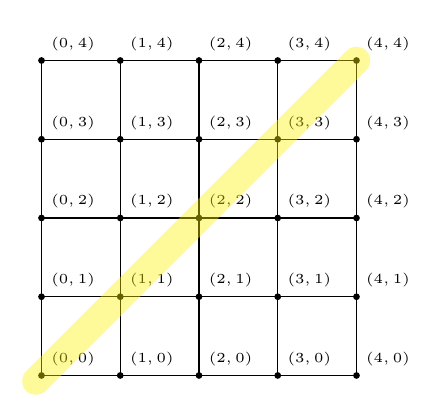
\begin{tikzpicture}
			[strip/.style = {
				draw=#1,
				line width=1em, opacity=0.4,
				line cap=round ,
			}]
			\draw[step=1.0,black,thin] (0,0) grid (4,4);
			\foreach \x in {0,...,4}
			\foreach \y in {0,...,4}
			\filldraw (\x,\y) circle[radius=1pt] node[above right] {\tiny $(\x,\y)$};
			\path[draw,strip=yellow,shorten <=-1mm] (0,0) -- (4,4);
		\end{tikzpicture}
	\end{center}
\end{example}

\begin{example}
	Tra le relazioni binarie in un insieme $s$ vi sono la \textbf{relazione identica} $\iota_{s} = (s,s, \Delta_{s})$ e la \textbf{relazione totale} $\tau_{s}=(s,s,s \times s)$. È chiaro che nella relazione identica ogni elemento è in relazione soltanto con se stesso mentre nella relazione totale ogni elemento di $s$ è in relazione con ciascun elemento.
\end{example}

\subsection{Proprietà delle relazioni binarie}
\begin{defbox}{Relazione opposta}\index{Relazione opposta}
	Sia $\rho = (s,s,G)$ una relazione binaria nell'insieme non vuoto $s$ e si ponga $G^{*}=\{(y,x)\;|\; (x,y) \in G\}$. Allora la coppia $\rho^{*}=(s,s,G^{*})$ è una relazione binaria in $s$ che prende il nome di \textbf{relazione opposta} di $\rho$.
\end{defbox}

Sia $s$ un insieme non vuoto. Per una relazione binaria $\rho = (s,s,G)$ in $s$ si danno le seguenti definizioni:
\begin{itemize}
	\item $\rho$ si dice \textbf{riflessiva} se	$\forall x \in s (x \ \rho \ x)$, cioè se il grafico $G$ contiene la diagonale $\Delta_{s}$;
	\item $\rho$ si dice \textbf{antiriflessiva} se $\forall x \in s \; (x \ \cancel{\rho} \ x)$, cioè se il grafico $G$ è disgiunto dalla diagonale $\Delta_{s}$;
	\item $\rho$ si dice \textbf{simmetrica} se per ogni coppia $(x,y)$ di elementi di $s$ tali che $x \ \rho \ y$ si ha anche $y \ \rho \ x$, cioè se $\rho$ coincide con la sua relazione opposta $\rho^{*}$.
	\item $\rho$ si dice \textbf{asimmetrica} se da $x \  \rho  \ y$ e $y \rho x$ segue $x=y$.
	\item $\rho$ si dice \textbf{transitiva} se qualunque siano gli elementi $x$, $y$ e $z$ di $s$ tali che $x \ \rho \ y$ e $y \ \rho \ z$, si ha anche $x \ \rho \ z$.
\end{itemize}

\subsection{Rappresentazione delle corrispondenze}

\begin{example}
	Dati $A=\{0,1,2\}$ e $b=\{0,4\}$ si avrà che l'insieme $A \times b$ conterrà le coppie ordinate:
	\begin{displaymath}
		A \times b = \{(0,0),(0,4),(1,0),(1,4),(2,0),(2,4)\}
	\end{displaymath}
	Dunque esisteranno $2^{6}=64$ sottoinsiemi del prodotto cartesiano, ovvero 64 diverse tipologie di corrispondenze tra gli insiemi $A$ e $b$. Per descrivere dunque una corrispondenza può essere comodo esprimere la \textbf{condizione di appartenenza} al grafico della corrispondenza. Ad esempio il grafico:	$G = \{(x,y) \in A \times b \; | \; x < y \}$ esprime l'insieme:
	\begin{displaymath}
		G = \{(0,4),(1,4),(2,4)\} \subset A \times b
	\end{displaymath}
	Che descrive la seguente definizione di corrispondenza:
	\begin{displaymath}
		\alpha \in Corr(A,b) \qquad \mbox{definito da} \quad \forall x \in A \; \forall y \in b \quad \bigl( x \; \alpha \; y \iff x <y \bigr)
	\end{displaymath}
\end{example}

\begin{example}
	Oltre a rappresentare una corrispondenza mediante il proprio grafico è possibile utilizzare anche una rappresentazione grafica mediante i diagrammi di Venn oppure mediante tabelle. Si considerino gli insiemi $A=\{1,2,3\}$, $b=\{x,y\}$ e la corrispondenza $\rho=(A,b,\{(1,x),(1,y),(3,y)\})$. Si hanno quindi le seguenti rappresentazioni:
	\begin{center}
		\begin{minipage}{.45\textwidth}
			\centering
			\begin{tikzpicture}
				\filldraw[black] (0,0) circle (2pt) node[anchor=west] (1) {$1$};
				\filldraw[black] (0,-1) circle (2pt) node[anchor=west] (2) {$2$};
				\filldraw[black] (0,-2) circle (2pt) node[anchor=west] (3) {$3$};
				\filldraw[black] (4,-1) circle (2pt) node[anchor=west] (4) {$x$};
				\filldraw[black] (4,-2) circle (2pt) node[anchor=west] (5) {$y$};
				\node[shape=ellipse,minimum width=2cm,draw=blue,fit={(1)(2)(3)},,label=above:$A$](e3){};
				\node[shape=ellipse,minimum width=2cm,draw=green,fit={(4)(5)},label=above:$b$]{};
				\draw[->,xshift=-5pt](1)to[bend left=25](4,-1);
				\draw[->,xshift=-5pt](1) to [bend right=25](4,-2);
				\draw[->,xshift=-5pt](3) to [bend right =25] (4,-2);
			\end{tikzpicture}
			\captionof{figure}{Diagrammi di Venn}
		\end{minipage}
		\hfil
		\begin{minipage}{.45\textwidth}
			\centering
			\begin{tblr}
				{
					hline{1-Z} = {0.9pt},
					vline{1-Z} = {0.9pt},
					vline{1} = {1}{0pt},
					hline{1} = {1}{0pt},
					cell{1}{2-Z}={primary!40!white},
					cell{2-Z}{1}={primary!40!white}
				}
				& $x$ & $y$ \\
				1 & $\bullet$ & $\bullet$ \\
				2 & & \\
				3 & & $\bullet$
			\end{tblr}
			\captionof{table}{Rappresentazione tabellare}
		\end{minipage}
	\end{center}
\end{example}

\subsection{Prodotto relazionale}\label{prodotto_relazionale}

\begin{defbox}{Prodotto relazionale}
	Siano $A,B,C$ insiemi e $\varphi \in Corr(A,B)$, e $\psi \in Corr(B,C)$ corrispondenze. Il \textbf{prodotto relazionale} di $\varphi$ per $\psi$, denotata con $\varphi \psi$, è la corrispondenza definita ponendo:
	\begin{equation}
		\forall a \in A, \forall c \in C \qquad a \ \varphi \psi \ c \iff \Bigl( \exists b \in B \bigl( (a \ \varphi \ b) \wedge (b \ \psi \ c)\bigr)\Bigr)
	\end{equation}
	
\end{defbox}

\begin{teorbox}[Associatività del prodotto relazionale]
	Il prodotto relazionale gode della proprietà associativa, cioè se:
	$\alpha \in Corr(A, B), \ \beta \in Corr(B,C), \ \gamma \in Corr(C,D)$	sono corrispondenze, allora vale:
	\begin{equation}
		(\alpha \beta) \gamma = \alpha(\beta \gamma)
	\end{equation}
\end{teorbox}

\begin{proof}
	Deve essere, per ogni $a \in A$ e per ogni $d \in D$:
	\begin{align*}
		a \ (\alpha \beta) \ \gamma d & \iff \exists c \in C \bigl( a \ \alpha \beta \ c \wedge c \ \gamma \ d \bigr)  \\
		& \iff \exists c \in C \bigl( \exists b \in B (a \ \alpha \ b \wedge b \ \beta \ c) \wedge c \ \gamma \ d \bigr) \\
		& \iff \exists c \in C, \exists b \in B \bigl(a \ \alpha \ b \wedge b \ \beta \ c \wedge c \ \gamma \ d\bigr)
	\end{align*}
	Analogamente:
	\begin{align*}
		a \ \alpha (\beta \gamma) \ d & \iff \exists b \in B \bigl(a \ \alpha \ b \wedge b \ \beta\gamma \ d \bigr)\\
		& \iff \exists b \in B \Bigl( a \ \alpha \ b \wedge \bigl(\exists c \in C (b \ \beta \ c \wedge c \ \gamma \ d) \bigr) \Bigr) \\
		& \iff \exists b \in B, \exists c \in C \bigl( a \ \alpha \ b \wedge b \ \beta \ c \wedge c \ \gamma \ d \bigr)
	\end{align*}
	Dato che le due condizioni sono equivalenti quindi le due corrispondenze coincidono.
\end{proof}

Per ogni insieme $A,B$ e per ogni corrispondenza $\alpha \in Corr(A,B)$ è possibile considerare i prodotti $id_{A}\alpha$ e $\alpha id_{B}$: $$A \stackrel{id_{A}}{\longrightarrow} A \stackrel{\alpha}{\longrightarrow} B \stackrel{id_{B}}{\longrightarrow} B$$E vale: $id_{A}\alpha = \alpha = \alpha id_{B}$. Infatti:
\begin{displaymath}
	x \ \alpha \ b  \implies \bigl( x \ id_{A} \ x \wedge x \ \alpha \ b \bigr) \implies x \ (id_{A} \alpha) \ b
\end{displaymath}
e:
\begin{displaymath}
	x \ (id_{A} \alpha) \ b \implies  \exists y \in A \Bigl( x \ id_{A} \ y \wedge y \ \alpha \ b \Bigr) \implies x \ \alpha \ b
\end{displaymath}
Analogamente, per ogni $x \in A$ e $b \in B$:
\begin{displaymath}
	x \ \alpha \ b \implies \Bigl( x \ \alpha \ b \wedge b \ id_{B} \ b\Bigr) \implies x \ \alpha id_{B} \ b
\end{displaymath}
e
\begin{displaymath}
	x \ \alpha id_{B} \ b \implies \exists c \in B \Bigl( x \ \alpha \ c \wedge c \ id_{B} \ b \Bigr) \implies x \ \alpha \ b
\end{displaymath}

\section{Applicazioni}

\begin{defbox}{Applicazione}\index{Applicazione}
	Un'\textbf{applicazione} (o \textit{funzione} o \textit{mappa}) di $A$ in $B$ è una corrispondenza $\varphi \in Corr(A,B)$ con la seguente proprietà:
	\begin{equation}\label{eq:applicazione}
		\forall x \in A \quad ( \exists! \ y \in B (x \ \varphi \ y))
	\end{equation}
\end{defbox}

Per indicare che $\varphi$ è un'applicazione di $A$ in $B$ scriveremo: $\varphi: A \rightarrow B$ oppure $ A \stackrel{\varphi}{\rightarrow} B$. Per indicare che all'elemento $a \in A$ corrisponde l'unico elemento $b \in  B$ scriveremo $\varphi(a)=b$ oppure $\varphi:a \mapsto b$, $b$ è chiamata ``\textbf{immagine} di $a$ mediante $\varphi$''. L'insieme $A$ prende il nome di \textbf{dominio} dell'applicazione mentre l'insieme $B$ viene chiamato \textbf{codominio}.

\begin{example}
	\begin{enumerate}
		\item La $f$ assegni a ogni numero reale il suo quadrato, si abbia cioè, per ogni $x \in \mathbb{R} \bigl(f(x)=x^{2}\bigr)$. Dominio e codominio di $f$ sono i numeri reali.
		\item La $f$ associa ogni nazione la rispettiva capitale. Ora il dominio di $f$ è l'insieme delle nazioni, e il suo codominio l'insieme delle città.
	\end{enumerate}
\end{example}

\begin{defbox}{Mappa}
	L'insieme delle funzioni dall'insieme $A$ all'insieme $B$ viene chiamato \textbf{mappa} e si indica col simbolo: $$Map(A,B)= \{ \varphi \; | \; \varphi: A \rightarrow B \}$$ Altre notazioni possibili sono quella esponenziale: $B^{A}$ oppure $t(A,B)$.
\end{defbox}

\begin{center}
	\begin{tikzpicture}
		\node[shape=ellipse,draw=blue, minimum height=3cm, minimum width=4cm] (a) {$A$};
		\node[shape=ellipse, draw=blue, minimum height=2cm, minimum width=3cm, right=4cm of a] (b) {$B$};
		\draw[->] (a) to node[above,midway]{$f$} (b);
	\end{tikzpicture}
\captionof{figure}{Diagramma di una mappa dall'insieme $A$ all'insieme $B$}
\end{center}

\begin{osservation}
	Definite le funzioni come terne ordinate si avrà, in base alla Proposizione~\ref{prop_terne_ordinate}, che due funzioni $f=(A,B,G_{f})$ e $g=(C,D,G_{g})$ si diranno equivalenti se, e soltanto se, hanno lo stesso dominio ($A=c$), lo stesso codominio ($B=D$) e lo stesso grafico ($G_{f}=G_{g}$).
\end{osservation}

Spesso per assegnare una funzione $ f\colon A \longrightarrow B$ si fornisce una ``legge'' ossia una qualche formula che permette di associare A ciascun elemento del dominio la sua immagine. Si faccia però attenzione al fatto che la funzione è caratterizzata soltanto dal dominio $A$, dal codominio $B$ e dal grafico $G$ e non dalla eventuale “formulazione della legge”. I due esempi seguenti mostrano come una stessa “legge” può definire funzioni diverse e come, d’altra parte, “leggi” diverse possono definire una stessa funzione.

\begin{example}
\begin{enumerate}
	\item La funzione $f\colon \mathbb{Z}\longrightarrow \mathbb {N}$ data da $f(n)=n^2$ e la funzione $g\colon \mathbb {N} \longrightarrow \mathbb {Z}$
	data da $g(n)=n^2$ sono diverse, perché non hanno lo stesso dominio e lo stesso	codominio, ma, oltre a questo, hanno anche proprietà molto diverse. Usando la terminologia che definiremo in seguito, $f$ non è iniettiva, mentre $g$ lo è.

	\item Siano $A=\{0,1,2\}$ ed $f,g: A \longrightarrow \mathbb{R}$ le funzioni definite rispettivamente da $f(x)=x-7$ e $g(x)=x^3-3x^2+3x-7$. Queste funzioni, per quanto espresse mediante ``leggi'' diverse, sono la stessa funzione, ossia $f=g$, poiché hanno lo stesso dominio, lo stesso codominio e lo stesso grafico: $G_{f} = G_{g} = \{(0,-7),(1,-6),(2,-5)\}$.
\end{enumerate}
\end{example}

\subsection{Questione della ``buona posizione'' delle applicazioni}
Solitamente si trovano notazioni del tipo: $x \in A \mapsto y \in B$
per indicare una funzione $t=(A \times b, G)$ dove: $G=\{(x,y) \; | \; x \in A, y \in B \}$ è il grafico della funzione. È importante saper distinguere le varie notazioni, infatti:
\[
\begin{array}{lc}
	\mathbb{N} \rightarrow \mathbb{Z} \qquad \mbox{viene utilizzata per le corrispondenze tra insiemi} \\
	n \mapsto n+1 \quad \mbox{è la notazione per indicare il valore associato all'elemento n}          \\
\end{array}
\]

È possibile trovare anche notazioni più complicate:
$$
s(x,y,z,...) \in A \mapsto t(x,y,z,...) \in B
$$
dove $s(x,y,z,...)$ è una espressione nelle variabili $(x,y,z,...)$. Non è sempre detto, però, che tali notazioni stiano ad indicare delle vere e proprie applicazioni ``ben definite''. Non sempre l'espressione $s(x,y,z,...)$ è \textit{descrittiva di tutti gli elementi del dominio}, così facendo si otterrebbero elementi del dominio che non godono di corrispondente e questo non va bene secondo la definizione di applicazione. Analogamente, $t(x,y,z,..)$ \textit{deve associare uno ed uno solo elemento del codominio}.

\begin{example}
	Analizziamo le corrispondenze rappresentate dai seguenti grafici:
	\begin{center}
		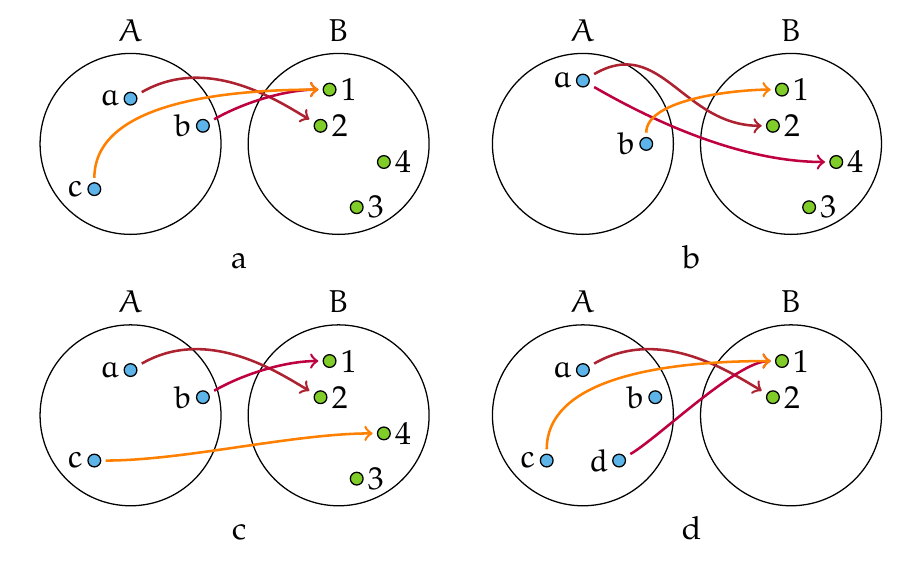
\includegraphics[scale=.55]{res/Corrispondenze_applicazioni.png}
	\end{center}
	La corrispondenza di figura a rappresenta una funzione.
	La corrispondenza di figura b non rappresenta una funzione perché l’elemento $a$ di $A$ è in corrispondenza con due elementi di $B$, il 2 e il 4, quindi non è una corrispondenza univoca. La corrispondenza della figura c rappresenta una funzione. La corrispondenza della figura d non è una funzione perché il dominio non coincide con l’insieme $A$.
\end{example}

\begin{example}
	L'applicazione: $\beta: x \in \mathbb{N} \mapsto x+1 \in \mathbb{Z}$ è ben posta in quanto per ogni elemento $x \in \mathbb{N}$ esiste ed è unico il suo successivo definito in $\mathbb{Z}$.
\end{example}

\begin{example}
	La corrispondenza $\alpha: n \in \mathbb{N} \mapsto n-1 \in \mathbb{N}$ non è un'applicazione. Infatti l'elemento $0 \in \mathbb{N}$ non ammette precedente. Quando verifichiamo la buona posizione di una applicazione dobbiamo verificare che \textbf{tutti} i valori del dominio abbiano un corrispondente del codominio.
\end{example}

\begin{example}
	La notazione $(a,b) \in \mathbb{R}\times \mathbb{R} \mapsto \frac{a}{b} \in \mathbb{R} $
	non descrive una applicazione in quanto tutte le coppie di seconda coordinata nulla non hanno un loro corrispondente.
\end{example}

\begin{example}
	L'applicazione $n \in \mathbb{N} \mapsto n-1 \in \mathbb{Z}$ è un'applicazione dato che l'insieme di arrivo è quello dei numeri interi.
\end{example}

\begin{example}
	La corrispondenza $X \in \mathcal{P}(\mathbb{Z}) \mapsto X \cap \mathbb{N}\in \mathcal{P}(\mathbb{N})$ è un'applicazione. Infatti ogni parte dell'insieme dei numeri interi, se intersecata con l'insieme dei numeri naturali, è una parte dell'insieme $\mathbb{N}$. Al contrario, la corrispondenza $\{x\}\in \mathcal{P}(\mathbb{Z}) \mapsto \{x\}\cap \mathbb{N} \in \mathcal{P}(\mathbb{N})$ non è un'applicazione. Infatti l'espressione $\{x\}\in \mathcal{P}(\mathbb{Z})$ non è \textit{descrittiva} di tutti gli elementi del dominio $\mathcal{P}(\mathbb{Z})$, esistono quindi elementi che non hanno corrispondenti secondo la formula.
\end{example}

\begin{example}
	La relazione:
	$$
	f=(\mathbb{R} \times \mathbb{R},G) \qquad G=\{(x,y) \in \mathbb{R}^{2} \; | \; y^{2}=x \}
	$$
	non è una funzione poiché contraddice la definizione di applicazione in quanto esistono sempre due numeri $y_{1},y_{2}$ tali che $y_{1}^{2}=y_{2}^{2}=x$, ad esempio $(-2)^{2}=2^{2}=4$.
\end{example}

\begin{example}
	$\{a,b\} \in \mathcal{P}(\mathbb{Z}) \mapsto a+b \in \mathbb{Z}$ \textbf{non} è una funzione poiché non tutti gli elementi del dominio hanno una propria immagine.
	Fissato invece, per ogni insieme $A$ e per ogni naturale $k$, l'insieme:
	\begin{equation}
		\mathcal{P}_{k}(A)=\{X \in \mathcal{P}(A) \ | \ |X|=k\}
	\end{equation}
	
	detto l'\textit{insieme delle parti di $A$ di cardinalità $k$}. Possiamo considerare quindi:
	\[
	\begin{array}{lc}
		p: \{a,b\} \in \mathcal{P}_{2}(\mathbb{Z}) \mapsto a+b \in \mathbb{Z} \\
		q: \{a,b\} \in \mathcal{P}_{2}(\mathbb{Z}) \mapsto a-b \in \mathbb{Z}
	\end{array}
	\]
	Mentre $p$ è una applicazione, $q$ non lo è. Infatti elementi uguali di $\mathcal{P}_{2}(\mathbb{Z})$ hanno immagini distinte: ad esempio l'insieme $\{1,2\}$ può essere riscritto anche come $\{2,1\}$ ma $$q(\{1,2\})=-1 \neq  q(\{2,1\})=1$$
\end{example}

\begin{example}
	Analogamente all'esempio precedente si ha che: $(a,b)\in \mathbb{N}^{2} \mapsto a-b \in \mathbb{N}$ \textbf{non è} una applicazione mentre la relazione: $(a,b) \in \mathbb{Z}^{2} \mapsto a-b \in \mathbb{Z}$ lo è.
\end{example}


\begin{defbox}{Insieme immagine}
	Si definisce \textbf{immagine} dell'insieme $A$ mediante l'applicazione $\varphi$ l'insieme:
	\begin{equation}
		Im \ \varphi = \{ \varphi(x)\; | \; x \in A \}
	\end{equation}
\end{defbox}

\begin{example}
	Sia dato $X=\{1,2,3\}$ e sia $f:x \in X \mapsto \sqrt{x^{2}+3} \in \mathbb{R}$ e si voglia determinare l'insieme immagine della funzione $f$. In questo caso basta sostituire uno alla volta gli elementi del dominio nell'espressione di $f$ e svolgere dei semplici passaggi algebrici:
	\begin{displaymath}
		\begin{array}{l}
			f(1)=\sqrt{1^{2}+3}=\sqrt{4}=2 \\
			f(2)=\sqrt{2^{2}+3}=\sqrt{7}   \\
			f(3)=\sqrt{3^{2}+3}=\sqrt{12}
		\end{array}
	\end{displaymath}
\end{example}

\begin{example}
	Sia dato $X=\mathbb{R}$ e $f:x \in X \mapsto x+1 \in \mathbb{R}$. Per determinare l'insieme immagine $Im(f)$ esplicitiamo la $x$ in funzione della $y$:
	\begin{displaymath}
		\begin{array}{ll}
			y = x+1 & \text{\textcolor{gray}{Sposto il $+1$ A sinistra e inverto il segno}} \\
			x = y-1 &                                                                       \\
		\end{array}
	\end{displaymath}
	Che ha soluzione su tutto $\mathbb{R}$ e tra l'altro coincide con il codominio della funzione, ovvero $Im(f)= cod(f)=\mathbb{R}$.
\end{example}


\begin{defbox}{Funzione costante}\index{Applicazione!Costante}
	Siano $A,B$ insiemi e sia $f \in Map(A,B)$. $f$ si dice \textbf{costante} se e solo se
	\begin{equation}
		f(x)=f(y) \quad \forall x,y \in A
	\end{equation}
	
	Fissato $h \in B$, l'applicazione $x \in A \mapsto h \in B$ si dice \textbf{funzione costante $h$}.
\end{defbox}

\begin{example}
	Un esempio di applicazione costante è l'applicazione costante $c_{0}$ che associa ad ogni numero naturale l'elemento $0 \in \mathbb{N}$:
\end{example}


\begin{defbox}{Restrizione}\index{Restrizione}
	Sia A un insieme, $f \in Map(A,B)$ e $T \subseteq A$. Possono definire una applicazione $r \in Map(T,B)$ come:
	\begin{equation}
		f_{\vert_{T}}:	x \in T \mapsto f(x) \in B
	\end{equation}
	Questa applicazione è ben definita e si chiama \textbf{restrizione} di $f$ a $T$.
\end{defbox}


\begin{example}
	Sia: $\alpha: n \in \mathbb{Z} \mapsto n^{2}+1 \in \mathbb{N}$.	Un esempio di restrizione si ottiene cambiando l'insieme di partenza con $\mathbb{N} \subset \mathbb{Z}$, ottenendo così l'applicazione:
	\begin{displaymath}
		\alpha_{\vert_{\mathbb{N}}}: n \in \mathbb{N} \mapsto n^{2}+1 \in \mathbb{N}
	\end{displaymath}
\end{example}


\begin{defbox}{Prolungamento}\index{Prolungamento}
	Se $g: T \subseteq A \longrightarrow B $ è la restrizione di $f: A \longrightarrow B$, allora $f$ viene detta \textbf{prolungamento} dell'applicazione $g$.
\end{defbox}



\begin{defbox}{Immersione}\index{Immersione}
	Per ogni insieme $A$ e per ogni $T \subseteq A$, l'applicazione:
	\begin{equation}
		\iota:	x \in T \mapsto x \in A
	\end{equation}
	viene chiamata \textbf{immersione di $T$ in $A$} e si denota col simbolo $\iota \coloneqq T \hookrightarrow A$.
\end{defbox}



\begin{osservation}
	L'immersione è la \textit{restrizione dell'applicazione identica $id_{A}$} all'insieme $T \subseteq A$. Inoltre, per ogni applicazione $f: A \longrightarrow B$ si ha:
	\begin{displaymath}
		f \circ \iota = f( \iota(x))= f(x)
	\end{displaymath}
	Quindi $f \circ \iota : x \in T \mapsto f(x) \in B$ è proprio $f_{\vert_{T}}$. Quindi una restrizione si ottiene componendo una applicazione con una immersione.
	
\end{osservation}

\begin{example}
	L'applicazione identica $id_{A}$ è un'immersione di $A$ in $A$:
	\begin{displaymath}
		id_{A} = A \hookrightarrow A
	\end{displaymath}
	Ogni applicazione $f: A \longrightarrow B$ può essere considerata come restrizione di sé stessa rispetto all'insieme $A$: $f = f_{\vert_{A}}$.
\end{example}


\begin{defbox}{Applicazione ridotta}\index{Applicazione!Ridotta}
	Sia $f:A\rightarrow B$, per ogni sottoinsieme $C \subseteq B$ tale che $im \ f \subseteq C$, l'applicazione:
	\begin{equation}
		x \in A \mapsto f(x)\in C
	\end{equation}
	si chiama \textbf{ridotta} di $f$ a $C$ e si indica col simbolo $f^{\vert C}$.
\end{defbox}



\begin{defbox}{Applicazione immagine}\index{Applicazione!Immagine}
	Siano $a,b$ due insiemi ed $f : A \rightarrow B$ un'applicazione. L'applicazione:
	\begin{equation}
		\overrightarrow{f} : C \in \mathcal{P}(A) \mapsto \{f(x) \; | \; x \in C \} \in \mathcal{P}(B)
	\end{equation}
	è chiamata \textbf{applicazione immagine} definita da $f$.
\end{defbox}



\begin{propbox}
	Siano $A$ e $B$ due insiemi e consideriamo l'applicazione $f: A \rightarrow B$. Per ogni $C \in \mathcal{P}(A)$:
	\begin{eqnarray}
		\overrightarrow{f}(C) &= Im (f_{\vert C}) = \{ f(x) \; | \; x \in C \} \\
		\overrightarrow{f}(A) &= Im (f)
	\end{eqnarray}
\end{propbox}

Ovvero:
\begin{itemize}
	\item L'applicazione immagine di un sottoinsieme $C \subseteq A$ è l'insieme immagine della restrizione dell'applicazione $f$ all'insieme $C$;
	\item L'applicazione immagine del dominio coincide con l'insieme immagine dell'applicazione $f$.
\end{itemize}

\begin{example}
	Sia $f: n \in  \mathbb{Z} \mapsto |n| \in \mathbb{N}$ e sia $X= \{ 0,1,-1\}$, allora $\overrightarrow{f}(X)=\{0,1\}$.
\end{example}


\begin{defbox}{Applicazione antimmagine}\index{Applicazione!Antimmagine}
	Siano $A,B$ due insiemi ed $f : A \rightarrow B$ un'applicazione. Si definisce \textbf{applicazione antimmagine} definita da $f$ l'applicazione:
	\begin{equation}
		\overleftarrow{f} :C \in \mathcal{P}(B) \mapsto \{ x \in A \; | \; f(x) \in C \} \in \mathcal{P}(A)
	\end{equation}
\end{defbox}

\begin{propbox}
	Siano $A,B$ insiemi e sia $f: A \rightarrow B$ un'applicazione di $A$ in $B$. Allora:
	\begin{equation}
		\overleftarrow{f}(B) = \{x \in A \; | \; f(x) \in B \} = A = \overleftarrow{f}(im \ f)
	\end{equation}
\end{propbox}

Ovvero, l'antimmagine del codominio $B$ coincide con il dominio $A$ che a sua volta coincide con l'antimmagine dell'insieme immagine dell'applicazione $f$. Ovviamente si ha anche che: $\overleftarrow{f}(\varnothing) = \varnothing$.

\begin{example}
	Sia $f: n \in  \mathbb{Z} \mapsto |n| \in \mathbb{N}$, allora se consideriamo il sottoinsieme $\{1,2,3\} \subseteq \mathbb{N}$ si ha:
	\begin{displaymath}
		\overleftarrow{f} \bigl(\{1,2,3\}\bigr)=\{-1,1,-2,2,-3,3\}
	\end{displaymath}
\end{example}

Le proprietà seguenti saranno importanti per poter caratterizzare le applicazioni iniettive e suriettive. Siano infatti $A,B$ due insiemi non vuoti e sia $f: A \rightarrow B$. È opportuno notare che in generale risulta:
\begin{align*}
	\forall C \in \mathcal{P}(A) \bigl(C \neq \overleftarrow{f}(\overrightarrow{f}(C)) \bigr) \\
	\forall Y \in \mathcal{P}(B) \bigl( Y \neq \overrightarrow{f}(\overleftarrow{f}(Y))\bigr)
\end{align*}
 Se $C$ è una parte di $A$ e $x \in C$, si ha $f(c) \in \overrightarrow{f}(C)$ e quindi $x \in \overleftarrow{f}(\overrightarrow{f}(C))$. Quindi $C \subseteq \overleftarrow{f}(\overrightarrow{f}(C))$ (l'inclusione può essere stretta come mostrato nel prossimo esempio). Sia invece $Y$ un sottoinsieme del codominio $B$ di $f$. Qualunque sia l'elemento $z$ di $\overrightarrow{f}(\overleftarrow{f}(Y))$ risulta $z=f(x)$ con $x \in \overleftarrow{f}(Y)$. Allora $z = f(x)$ appartiene a $Y$ e perciò $\overrightarrow{f}(\overleftarrow{f}(Y)) \subseteq y$. In particolare $\overrightarrow{f}(\overleftarrow{f}(Y)) = Y \cap im \ f$.


\begin{example}
	Sia $T=\{3\}$ e sia $f: n \in \mathbb{Z} \mapsto n^{2} \in \mathbb{Z}$. Allora: $$\overrightarrow{f}(\{3\}) = \{f(x)/x \in \{3\}\} = \{9\}$$ e $$\overleftarrow{f}(\overrightarrow{f}(\{3\})) = \overleftarrow{f}(\{9\}) =\{n \in \mathbb{Z} \; | \; 9 = n^{2}\} = \{+3,-3\}$$ e vale $T \subset \overleftarrow{f}(\overrightarrow{f}(T))$.
\end{example}

\subsection{Composizione tra applicazioni}


\begin{propbox}
	Supponiamo di avere due applicazioni componibili come corrispondenze. Siano quindi:
	\begin{displaymath}
		\begin{array}{l}
			\alpha: A \longrightarrow B \\
			\beta: B \longrightarrow C
		\end{array}
	\end{displaymath}
	due applicazioni siffatte. Allora $\alpha\beta$ è ancora un'applicazione, chiamata \textbf{applicazione composta}.
\end{propbox}


\begin{center}
	\begin{tikzpicture}[line width=1pt,>=latex]
		\filldraw[black] (0,0) circle (2pt) node[anchor=west] (a) {$a$};
		\filldraw[black] (2,0) circle (2pt) node[anchor=west] (b) {$b$};
		\node[shape=ellipse,draw=blue,minimum width=3cm,minimum height=2cm,fit={(a)(b)}](e1){};
		
		\filldraw[black] (4.5,0) circle (2pt) node[anchor=west] (c) {$c$};
		\filldraw[black] (6,0) circle (2pt) node[anchor=west] (d) {$d$};
		\node[shape=ellipse,draw=blue,minimum width=3cm,minimum height=2cm,fit={(c)(d)}](e2){};
		
		\filldraw[black] (9.5,0) circle (2pt) node[anchor=west] (e) {$e$};
		\filldraw[black] (11,0) circle (2pt) node[anchor=west] (f) {$f$};
		\filldraw[black] (13,0) circle (2pt) node[anchor=west] (g) {$g$};
		\node[shape=ellipse,draw=blue,minimum width=3cm,minimum height=2cm,fit={(e)(f)(g)}](e3){};
		
		\node[anchor=north,font=\color{blue}\bfseries]at(e1.south){$A$};
		\node[anchor=north,font=\color{blue}\bfseries]at(e2.south){$B$};
		\node[anchor=north,font=\color{blue}\bfseries]at(e3.south){$C$};
		
		\draw[->](e1) -- (e2) node[midway,above]{$\alpha$};
		\draw[->](e2) -- (e3) node[midway,above]{$\beta$};
		\draw[->,out=45,in=125,looseness=0.55](e1.north) to node[above]{$\alpha\beta$} (e3.north);
	\end{tikzpicture}
	\captionof{figure}{Esempio di composizione delle applicazioni $\alpha:A \rightarrow B$ e $\beta: B \rightarrow C$}
\end{center}
\begin{proof}
	Per ogni $a \in A$ possiamo considerare l'elemento $\beta(\alpha(a)) \in C$. Quindi l'elemento $a \in A$ rispetto alla corrispondenza $\alpha \beta$ ha $\beta(\alpha(a)) \in C$ come corrispondente. Bisogna dimostrare che questo è unico stando alla definizione di applicazione.
	
	Supponiamo di avere $c \in C$ tale che sia un corrispondente rispetto a $\alpha \beta$ di $a \in A$. Ciò sta a significare che $\exists b \in B \bigl( a \ \alpha \ b \wedge b \ \beta \ c \bigr)$. Ma se $a \ \alpha \ b$ allora, per definizione di applicazione, $b= \alpha(a)$ e $c=\beta(b)=\beta(\alpha(a))$. Quindi per ogni elemento $a \in A$ esiste ed è unico il corrispondente $c \in C$ ovvero $\beta(\alpha(a))$. Ciò dimostra che $\alpha \beta$ è una applicazione.
\end{proof}

Spesso si usa indicare il prodotto relazionale $\alpha \beta$ con $\beta \circ \alpha$ dove $\circ$ indica il simbolo dell'operazione di prodotto relazionale.

La composizione tra applicazioni, così come il prodotto relazionale, non gode della proprietà commutativa. Non vale cioè, date due applicazioni $\alpha: a \rightarrow b$ e $\beta: b \rightarrow c$, $\alpha \beta = \beta \alpha$ o, equivalentemente, $\beta \circ \alpha = \alpha \circ \beta$. Infatti, continuando ad utilizzare la notazione ``cerchietto'', osserviamo che non esiste una applicazione del tipo $\alpha \circ \beta$ in quanto $\beta$ mappa ogni elemento dell'insieme $b$ nell'insieme $c$ mentre $\alpha$ è applicata solo e soltanto sugli elementi di $a$ e non ha senso quindi valutare l'espressione $\alpha (z)$ dove $z=g(y)$. La composizione tra applicazioni gode, però, della proprietà associativa come già osservato per le corrispondenze:


\begin{propbox}
	Siano $f: a \rightarrow b$, $g: b \rightarrow c$ e $h: c \rightarrow d$ tre applicazioni tra gli insiemi $a,b,c,d$. Vale allora:
	\begin{equation}
		f(gh)=(fg)h
	\end{equation}
	o, equivalentemente:
	\begin{equation}
		(h \circ g) \circ f = h \circ (g \circ f)
	\end{equation}
	
\end{propbox}

\begin{example}
	Sia:
	\begin{displaymath}
		\alpha: n \in \mathbb{Z} \mapsto n+1 \in \mathbb{Z}
	\end{displaymath}
	Allora:
	\begin{displaymath}
		\alpha^{2} = \alpha \alpha: n \in \mathbb{Z} \mapsto \alpha (\alpha(n)) \in \mathbb{Z}
	\end{displaymath}
	ovvero, per ogni $n \in \mathbb{Z}$ si ha: $\alpha (\alpha(n)) = \alpha(n+1)= (n+1)+1=n+2$. Sia ora:
	\begin{displaymath}
		\beta: m \in \mathbb{Z} \mapsto \{m\} \in \mathcal{P}(\mathbb{Z})
	\end{displaymath}
	un'applicazione. Allora $\alpha\beta= \beta \circ \alpha: \mathbb{Z} \longrightarrow \mathcal{P}(\mathbb{Z})$ e sarà:
	\begin{displaymath}
		\beta(\alpha(n))=\beta(n+1)=\{n+1\}
	\end{displaymath}
\end{example}

\begin{osservation}\label{osservation:non_commutativity_composition}
	Sia $s=\{x,y\}$ un insieme composto da due elementi distinti. È possibile quindi considerare le applicazioni costanti:
	\begin{displaymath}
		\begin{array}{l}
			c_{s,x} : a \in s \mapsto x \in s \\
			c_{s,y} : a \in s \mapsto y \in s
		\end{array}
	\end{displaymath}
	Componendole, si ottiene:
	\begin{displaymath}
		\begin{array}{l}
			c_{s,x} \circ c_{s,y} = c_{s,x} \\
			c_{s,y} \circ c_{s,x} = c_{s,y}
		\end{array}
	\end{displaymath}
	Da questo esempio si osserva inoltre che la composizione tra applicazioni non gode della proprietà commutativa. In particolare, se $|s|=2$ allora l'insieme delle trasformazioni in s, $s^{s}$, non è abeliano.
\end{osservation}

\section{Suriettività e iniettività}
\subsection{Funzioni iniettive}
\begin{defbox}{Applicazione iniettiva}
	Una funzione $f:a \rightarrow b$ si dice \textbf{iniettiva} se:
	\begin{equation}
		\forall \; x,y \in a \Bigl( x \neq y \implies f(x) \neq f(y) \Bigr)
	\end{equation}
	oppure
	\begin{equation}
		\forall \; x,y \in a \Bigl(f(x) = f(y) \implies x=y \Bigr)
	\end{equation}
\end{defbox}

Per farsi un'idea visivamente di cosa sia una applicazione iniettiva si può osservare il seguente diagramma:
\begin{center}
	\begin{tikzpicture}[line width=1pt,>=latex]
		\filldraw[black] (0,0) circle (2pt) node[anchor=west] (a) {$a$};
		\filldraw[black] (0,1) circle (2pt) node[anchor=west] (b) {$b$};
		\filldraw[black] (0,2) circle (2pt) node[anchor=west] (c) {$c$};
		\node[shape=circle,draw=blue,minimum width=3cm,minimum height=3cm,fit={(a)(b)(c)}](e1){};
		
		\filldraw[black] (5,0) circle (2pt) node[anchor=west] (d) {$d$};
		\filldraw[black] (5,1) circle (2pt) node[anchor=west] (e) {$e$};
		\filldraw[black] (5,2) circle (2pt) node[anchor=west] (f) {$f$};
		\node[shape=circle,draw=blue,minimum width=3cm,minimum height=3cm,fit={(d)(e)(f)}](e2){};
		
		\node[anchor=north,font=\color{blue}\bfseries]at(e1.south){$a$};
		\node[anchor=north,font=\color{blue}\bfseries]at(e2.south){$b$};
		
		\draw[->](a)--(e.175);
		\draw[->](b)--(d.190);
		\draw[->](c)--(f);
	\end{tikzpicture}
\end{center}
Si può notare infatti che ogni elemento di $a$ ha una immagine nel codominio $b$ diversa da quella di ciascun altro elemento.

\begin{osservation}
	Una applicazione $f: a \longrightarrow b$ non è iniettiva se e soltanto se:
	\begin{displaymath}
		\exists x,y \in a \bigl( x \neq y \wedge f(x)=f(y)\bigr)
	\end{displaymath}
	Ovvero se esistono elementi diversi di $a$ che hanno la medesima immagine.
\end{osservation}

\begin{example}
	L'applicazione $id_{a}$ è iniettiva. Se infatti $id_{a}(x)=id_{a}(y)$ allora $x=y$.
	\smallskip
	
	Sia $t \subset a$, l'immersione $\iota: x \in t \mapsto x \in a$ è iniettiva. Infatti, se $\iota(x)=\iota(y)$ allora $x=y$.
	\smallskip
	
	L'applicazione $\alpha: n \in \mathbb{Z} \mapsto n^{2} \in \mathbb{Z}$ non è iniettiva, infatti presi gli elementi distinti 1 e -1 si ha:
	\begin{displaymath}
		\alpha(-1) = \alpha(1)
	\end{displaymath}
	Al contrario, l'applicazione $\beta: n \in \mathbb{N} \mapsto n^{2} \in \mathbb{N}$ è iniettiva.
\end{example}


\begin{osservation}
	Se $f$ è un'applicazione iniettiva, per ogni $t \subseteq a$ allora la restrizione di $f$ a $t$:
	\begin{displaymath}
		f_{\vert_{t}}: x \in t \mapsto f(x) \in b
	\end{displaymath}
	è iniettiva. Infatti, presi due elementi $a,b \in t$ si ha, dall'iniettività di $f$
	\begin{displaymath}
		f(a) = f(b)  \implies a = b
	\end{displaymath}
	quindi vale in particolare anche per la restrizione di $f$ a $t$. Quindi $f_{\vert_{t}}$ è iniettiva.
\end{osservation}

\begin{propbox}[Caratterizzazione dell'iniettività mediante antimmagini]
	Un'applicazione $f:a \longrightarrow b$ è iniettiva, se e soltanto se
	\begin{displaymath}
		\forall y \in b \Bigl( |\overleftarrow{f}(\{y\})| \leq 1 \Bigr)
	\end{displaymath}
	Ovvero se e soltanto se per ogni singleton sottoinsieme del suo codominio, la sua antimmagine è vuota o ha un solo elemento.
\end{propbox}


\begin{proof}
	\begin{itemize}
		\item[$\implies$] Supponiamo che $f$ sia iniettiva e prendiamo un $y \in b$. Supponiamo che non sia vera la tesi, ovvero che l'antimmagine del singleton di $y$ non abbia al massimo un elemento. Se $|\overleftarrow{f}(\{y\})| \nleq 1$ allora esistono $a,b \in a$ tali che $a \neq b \wedge a,b \in \overleftarrow{f}(\{y\})$. Ma dire che $ a \in \overleftarrow{f}(\{y\})$ significa che $f(a)=y$ e $b \in \overleftarrow{f}(\{y\})$ che $f(b) =y$. Quindi $f(a)=f(b)$ con $a \neq b$ distinti e ciò va in contraddizione con la nostra ipotesi. Quindi $\overleftarrow{f}(\{y\})$ non può avere più di un elemento se $f$ è iniettiva.
		\item[$\impliedby$] Viceversa, se $f$ non è iniettiva, vale:
		\begin{displaymath}
			\exists x,y \in a \bigl( x \neq y \wedge f(x)=f(y)\bigr)
		\end{displaymath}
		Quindi, fissato $a,b \in a$ tali che $a \neq b \wedge f(a)=f(b)$, ponendo $y=f(a)$, abbiamo $a \in \overleftarrow{f}(\{y\})$ e anche $b \in \overleftarrow{f}(\{y\})$. Abbiamo così trovato due elementi diversi in $\overleftarrow{f}(\{y\})$ che avrà quindi più di un elemento. Di fatto, se $f$ non è iniettiva allora $\overleftarrow{f}(\{y\})$ avrà più di un elemento. Per contrapposizione si ottiene la tesi.
	\end{itemize}
\end{proof}

\begin{propbox}
	Siano $f:a \longrightarrow b$ e $g: b \longrightarrow c$ due applicazioni. Se $f,g$ sono iniettive allora anche l'applicazione $g \circ f$ è iniettiva.
\end{propbox}

\begin{proof}
	Siano $f: a \longrightarrow b$ e $g: b \longrightarrow c$ due funzioni iniettive. Siano $w,z \in a$ tali che $g \circ f(w) = g \circ f(z)$. Questo equivale a dire che $g(f(w)) = g(f(z))$. Essendo $g$ iniettiva, allora $f(w) = f(z)$. Ma, essendo $f$ iniettiva, allora $w=z$. Pertanto la funzione composta è iniettiva.
\end{proof}

\begin{propbox}
	Siano $f:a \longrightarrow b$ e $g: b \longrightarrow c$ due applicazioni. Se l'applicazione composta $g \circ f$ è iniettiva allora $f$ è iniettiva.
\end{propbox}
\begin{proof}
	Siano $x$ e $x'$ elementi di $a$ tali che $f(x)=f(x')$. Allora risulta:
	\begin{displaymath}
		(g \circ f)(x) = g(f(x)) = g(f(x'))=(g \circ f)(x')
	\end{displaymath}
	e quindi $x=x'$, in quanto $g \circ f$ è iniettiva. Pertanto $f$ è iniettiva.
\end{proof}

\subsection{Funzioni suriettive}
\begin{defbox}{Applicazioni suriettiva}
	L'applicazione $f$ si dice \textbf{suriettiva} se e solo se $im(f)=b$ e vale la seguente catena di implicazioni:
	\begin{eqnarray}\label{def:suriettività}
		im(f)=b &\iff & b \subseteq Im(f) \\
		& \iff & \forall y \in b ( y \in Im(f))  \\
		& \iff & \forall y \in b ( \exists x \in a ( y= f(x)))
	\end{eqnarray}
\end{defbox}

\begin{propbox}[Caratterizzazione suriettività mediante le antimmagini]
	Sia $f$ una applicazione da $a$ in $b$; $f$ è suriettiva se e soltanto se, per ogni $y \in b$:
	\begin{equation}
		\forall y \in b \Bigl( \overleftarrow{f}(\{y\}) \neq \emptyset \Bigr)
	\end{equation}
\end{propbox}

\begin{proof}
	Infatti, fissato un elemento $y \in b$ si ha sicuramente $\{y\} \subseteq b$, quindi ha senso considerare l'insieme:
	\begin{displaymath}
		\overleftarrow{f}(\{y\}) =\{x \in a \ | \ f(x) \in \{y\} \} = \{x \in a \ | \ f(x)=y\}
	\end{displaymath}
	Se la funzione $a \stackrel{f}{\longrightarrow}b$ è suriettiva allora sicuramente l'insieme degli elementi del dominio che hanno per immagine $y \in b$ è non vuoto. Vale cioè l'implicazione:
	\begin{displaymath}
		\forall y \in b \Bigl( y \in Im(f) \iff \bigl( \overleftarrow{f}(\{y\}\neq \emptyset)\bigr)\Bigr)
	\end{displaymath}
\end{proof}

\begin{osservation}
	Quando definiamo un concetto è importante fare qualche esempio. Per considerare una applicazione suriettiva è bene tenere a mente cosa \textit{non è} una applicazione suriettiva. Negando la definizione quindi si ottiene che una applicazione $f:a \longrightarrow b$ non è suriettiva se e soltanto se:
	\begin{itemize}
		\item $im \ f \neq b \iff b \nsubseteq im \ f$
		\item $\exists y \in b \Bigl( \forall x \in a \bigl(y \neq f(x) \bigr)\Bigr)$
		\item $\exists y \in b \setminus im \ f$
	\end{itemize}
\end{osservation}

\begin{example}
	L'applicazione identica in un insieme $a$ è suriettiva. Infatti $\forall a \in a (\exists a \in a (id_{a}(a)=a))$, ovvero $a$ stesso.
\end{example}

\begin{example}
	Se $t \subset a$ e consideriamo l'immersione $t \hookrightarrow a$ questa non è suriettiva in quanto esistono elementi del codominio che non sono immagine degli elementi del dominio.
\end{example}

\begin{example}
	L'applicazione $n \in \mathbb{Z} \mapsto n^{2} \in \mathbb{Z}$ non è suriettiva. Infatti non tutti i numeri interi possono essere espressi come quadrato di un numero intero relativo. Ad esempio il numero $5 \in \mathbb{Z}$.
\end{example}

\begin{example}
	L'applicazione $n \in \mathbb{Z} \mapsto |n| \in \mathbb{Z}$ non è suriettiva. Non tutti gli interi relativi possono essere espressi come il valore assoluto di un numero intero. Se però consideriamo la ridotta di tale applicazione:
	\begin{displaymath}
		n \in \mathbb{Z} \mapsto |n| \in \mathbb{N}
	\end{displaymath}
	questa è suriettiva in quanto ogni numero naturale rispetta tale condizione.
\end{example}
\begin{example}
	Diamo esempi grafici di un'applicazione suriettiva (Figura \ref{fig:suriettiva}) e di una non suriettiva (Figura \ref{fig:suriettiva2}).
	\begin{center}
		\begin{minipage}{.45\textwidth}
			\centering
			\begin{tikzpicture}[line width=1pt,>=latex]
				\filldraw[black] (0,0) circle (2pt) node[anchor=west] (a) {$a$};
				\filldraw[black] (0,1) circle (2pt) node[anchor=west] (b) {$b$};
				\filldraw[black] (0,2) circle (2pt) node[anchor=west] (c) {$c$};
				\node[shape=circle,draw=blue,minimum width=3cm,minimum height=2cm,fit={(a)(b)(c)}](e1){};
				
				\filldraw[black] (5,0) circle (2pt) node[anchor=west] (d) {$d$};
				\filldraw[black] (5,1) circle (2pt) node[anchor=west] (e) {$e$};
				\filldraw[black] (5,2) circle (2pt) node[anchor=west] (f) {$f$};
				\node[shape=circle,draw=blue,minimum width=3cm,minimum height=2cm,fit={(d)(e)(f)}](e2){};
				
				\node[anchor=north,font=\color{blue}\bfseries]at(e1.south){$a$};
				\node[anchor=north,font=\color{blue}\bfseries]at(e2.south){$b$};
				
				\draw[->](a)--(e.175);
				\draw[->](b)--(d.190);
				\draw[->](c)--(f);
				\draw[->](c)--(e.190);
			\end{tikzpicture}
			\captionof{figure}{}\label{fig:suriettiva}
		\end{minipage}
		\hfil
		\begin{minipage}{.45\textwidth}
			\centering
			\begin{tikzpicture}[line width=1pt,>=latex]
				\filldraw[black] (0,0) circle (2pt) node[anchor=west] (a) {$a$};
				\filldraw[black] (0,1) circle (2pt) node[anchor=west] (b) {$b$};
				\filldraw[black] (0,2) circle (2pt) node[anchor=west] (c) {$c$};
				\node[shape=circle,draw=blue,minimum width=3cm,minimum height=2cm,fit={(a)(b)(c)}](e1){};
				
				\filldraw[black] (5,0) circle (2pt) node[anchor=west] (d) {$d$};
				\filldraw[black] (5,1) circle (2pt) node[anchor=west] (e) {$e$};
				\filldraw[black] (5,2) circle (2pt) node[anchor=west] (f) {$f$};
				\node[shape=circle,draw=blue,minimum width=3cm,minimum height=2cm,fit={(d)(e)(f)}](e2){};
				
				\node[anchor=north,font=\color{blue}\bfseries]at(e1.south){$a$};
				\node[anchor=north,font=\color{blue}\bfseries]at(e2.south){$b$};
				
				\draw[->](a)--(e.175);
				\draw[->](b)--(d.190);
				\draw[->](c)--(e.190);
			\end{tikzpicture}
			\captionof{figure}{}\label{fig:suriettiva2}
		\end{minipage}
	\end{center}
\end{example}

In generale, per dimostrare la suriettività di una applicazione bisogna eseguire una dimostrazione che giustifichi la validità di una delle condizioni definite in \ref{def:suriettività}. Spesso però trovare una strategia vincente può risultare lungo e contorto. In questi casi le opzioni sono due: si procede per tentativi fino a quando non si trova un indizio sulla validità universale della condizione oppure si cerca un controesempio che dimostri che l'applicazione data non sia suriettiva.

\begin{example}
	Consideriamo l'applicazione:
	\begin{displaymath}
		\mu : x \in \mathcal{P}(\mathbb{Z}) \mapsto x \cap \mathbb{N} \in \mathcal{P}(\mathbb{N})
	\end{displaymath}
	Per dimostrare che questa applicazione sia suriettiva bisogna dimostrare che vale la condizione:
	\begin{equation}
		\forall y \in \mathcal{P}(\mathbb{N}) \Bigl(\exists x \in \mathcal{P}(\mathbb{Z}) \bigl( \mu(x) = y \bigr)\Bigr)
	\end{equation}
	Non sapendo come procedere inizio considerando un elemento a piacere di $\mathcal{P}(\mathbb{N})$, ad esempio $\{3\}$. La domanda che ci si pone sarà:
	\begin{quote}
		``Esiste una parte di $\mathbb{Z}$ la cui intersezione con $\mathbb{N}$ sia uguale a $\{3\}$?''
	\end{quote}
	Ovviamente sì e tale parte è $\{3\}$ stesso. Sostituendo a $\{3\}$ un qualsiasi elemento di $\mathcal{P}(\mathbb{N})$ notiamo che la risposta è sempre la stessa e quindi, generalizzando:
	\begin{displaymath}
		\forall y \in \mathcal{P}(\mathbb{Z}) \bigl( \mu(y)=y \cap \mathbb{N} = y \in \mathcal{P}(\mathbb{N}) \bigr)
	\end{displaymath}
\end{example}

\begin{propbox}
	Siano $a,b,c$ insiemi e $f: a \longrightarrow b$, $g: b \longrightarrow c$ due applicazioni. È possibile quindi considerare l'applicazione composta $g \circ f$. Allora, se $f,g$ sono suriettive anche $g \circ f$ è suriettiva.
\end{propbox}
\begin{proof}
	Se $f,g$ sono applicazioni suriettive, per dimostrare che la loro composta è suriettiva bisogna far vedere che:
	\begin{displaymath}
		\forall z \in C \Bigl(\exists x \in A \bigl(z=g \circ f (a)\bigr)\Bigr)
	\end{displaymath}
	Ma sappiamo che $g \circ f (a)= g(f(a))$ e per la suriettività dell'applicazione $g$:
	\begin{displaymath}
		\forall z \in C \bigl(\exists y \in B (z=g(y))\bigr)
	\end{displaymath}
	e per la suriettività di $f$ si ha:
	\begin{displaymath}
		\forall z \in C \bigl( \exists y \in B (\exists x \in A (z = g(f(x))))\bigr)
	\end{displaymath}
	il che dimostra la tesi.
\end{proof}

\begin{propbox}
	Se l'applicazione $g \circ f$ è suriettiva allora l'applicazione $g$ è suriettiva.
\end{propbox}

\begin{proof}
	L'obiettivo è quello di dimostrare che:
	\begin{displaymath}
		\forall x \in C \bigl( \exists y \in B (x= g(y))\bigr)
	\end{displaymath}
	Dato che $g \circ f$ è suriettiva sappiamo che:
	\begin{displaymath}
		\forall x \in C \bigl( \exists x' \in A (x = g\circ f(x'))\bigr)
	\end{displaymath}
	Quindi preso $y=f(x') \in B$ si ha:
	\begin{displaymath}
		c = g(f(x'))
	\end{displaymath}
	e quindi $g$ è suriettiva.
\end{proof}

\subsection{Funzioni biettive}
\begin{defbox}{Applicazione biettiva}
	Un'applicazione $a \stackrel{f}{\longrightarrow}b$ si dice \textbf{biettiva} se è sia iniettiva che suriettiva.
\end{defbox}

\begin{propbox}
	Un'applicazione $f: a \longrightarrow b$ è biettiva
	\begin{eqnarray}
		&\iff& \forall y \in b \Bigl( |\overleftarrow{f}(\{y\}| = 1)  \Bigr)  \\
		&\iff& \forall y \in b \Bigl ( \exists! \  x \in a \bigl (f(x) = y \bigl) \Bigl)
	\end{eqnarray}
\end{propbox}

\begin{corolbox}
	Siano $f:a \longrightarrow b$ e $g: b \longrightarrow c$ due applicazioni. Allora:
	\begin{enumerate}
		\item Se $f,g$ sono biettive allora $g \circ f$ è biettiva.
		\item Se $g \circ f$ è biettiva allora $g$ è suriettiva e $f$ è iniettiva.
	\end{enumerate}
\end{corolbox}

\section{Sezioni e Retrazioni}
\begin{defbox}{Sezione}
	Sia $f:a \longrightarrow b$. Si chiama \textbf{sezione} di $f$ un'applicazione $h: b \longrightarrow a$ tale che:
	\begin{equation}
		f \circ h = id_{b}
	\end{equation}
\end{defbox}

\begin{teorbox}\label{thm:car_sezioni}
	Un'applicazione $f:a \longrightarrow b$ è suriettiva se e solo se $f$ ha una sezione.
\end{teorbox}

\begin{proof}
	Supponiamo che esista una sezione $h:b \longrightarrow a$. Allora:
	\begin{displaymath}
		f \circ h = id_{b}
	\end{displaymath}
	è suriettiva in quanto $id_{b}$ è suriettiva. Quindi, essendo tale applicazione suriettiva si ha che $f$ è suriettiva.
	
	Viceversa se $f$ è suriettiva, sappiamo che:
	\begin{displaymath}
		\forall y \in b \bigl(\exists x \in a (y=f(x))\bigr)
	\end{displaymath}
	cioè:
	\begin{displaymath}
		\overleftarrow{f}(\{y\}) \neq \varnothing
	\end{displaymath}
	Quindi $\forall y \in b$ scegliamo un $a_{y} \in 	\overleftarrow{f}(\{y\})$ che sicuramente esiste in quanto non vuoto. È possibile quindi considerare l'applicazione:
	\begin{displaymath}
		f \circ h = f(h(y)) = f(a_{y}) = y = id_{b}(y)
	\end{displaymath}
	e quindi $h$ è una sezione di $f$.
\end{proof}

\begin{osservation}
	Dal teorema appena dimostrato concludiamo che se una applicazione $f:a \longrightarrow b$ non è suriettiva allora non ha sezioni.
\end{osservation}

\begin{example}
	L'applicazione $w: n \in \mathbb{Z} \mapsto |n| \in \mathbb{Z}$ non è suriettiva (i numeri interi negativi non possono essere espressi in termini di valore assoluto di un numero intero relativo) e quindi non ha sezioni. L'applicazione $v: n \in \mathbb{Z} \mapsto |n| \in \mathbb{N}$ è invece suriettiva e ammette sezioni. Ad esempio:
	\begin{displaymath}
		\sigma_{1}: n \in \mathbb{N} \mapsto n \in \mathbb{Z}
	\end{displaymath}
	è una sezione e vale: $v \circ \sigma_{1}(n)=v(\sigma_{1}(n))=v(n)=|n|=n=id_{\mathbb{N}}(n)$, analogamente anche l'applicazione:
	\begin{displaymath}
		\sigma_{2}: n \in \mathbb{N} \mapsto -n \in \mathbb{Z}
	\end{displaymath}
	è una sezione e vale: $v \circ \sigma_{2}(n)=v(\sigma_{2}(n))=v(-n)=|-n|=n=id_{\mathbb{N}}(n)$.
\end{example}

\begin{defbox}{Retrazione}
	Sia $f: a \longrightarrow b$ un'applicazione. Si chiama \textbf{retrazione} di $f$ un'applicazione $h: b \longrightarrow a$ tale che:
	\begin{equation}
		h \circ f = id_{a}
	\end{equation}
\end{defbox}

\begin{teorbox}\label{thm:car_iniettive}
	Un'applicazione $f: A \rightarrow B$ è iniettiva se e solo se $A=\varnothing$ oppure $f$ ha una retrazione.
\end{teorbox}

\begin{proof}
	\begin{itemize}
	\item[$\impliedby$] Se $f$ ha una retrazione allora è iniettiva, infatti, presa la retrazione $h: B \longrightarrow A$:
	\begin{displaymath}
		h \circ f = id_{A}
	\end{displaymath}
	con $id_{A}$ biettiva, quindi $f$ è iniettiva.
	
	\item[$\implies$] Sia $f$ iniettiva. Chiaramente, per ogni elemento $y \in im \ f$ si ha:
	\begin{displaymath}
		|\overleftarrow{f}(\{y\})|=1
	\end{displaymath}
	Allora $\exists ! \ a_{y} \in a \bigl( y=f(a_{y})\bigr)$
	Fissato $z \in a$ posso considerare l'applicazione:
	\begin{displaymath}
		h: y \in b \mapsto
		\begin{cases}
			a_{y} & \mbox{se }y \in im \ f     \\
			z     & \mbox{se } y \notin im \ f
		\end{cases}
		\in A
	\end{displaymath}
	Dimostriamo che $h$ è una retrazione di $f$. Per ogni $x \in a$ si ha:
	\begin{displaymath}
		(h \circ f) = h(f(x)) = a_{f(x)}
	\end{displaymath}
	dove $a_{f(x)}$ è l'unico elemento di $a$ tale che $f(a_{f(x)})=f(x)$ ovvero $x$ stesso. Quindi $h \circ f: A \longrightarrow A$ è un'applicazione che mappa ogni elemento in sé stesso. Di conseguenza $h \circ f = id_{A}$ ed $h$ è una retrazione di $f$.
	\end{itemize}
\end{proof}

\begin{example}
	Si consideri l'insieme $s=\{1,2,3\}$ e sia $t=\{1,2\}\subset s$ una parte propria di $s$. Dato che l'immersione $t \hookrightarrow s$ è una applicazione iniettiva allora questa applicazione ammette retrazioni. Ad esempio due possibili retrazioni di $\iota: x \in t \mapsto x \in s$ sono:
	\begin{displaymath}
		\begin{array}{ll}
			\rho_{1} :x \in s \mapsto \left\{ \begin{array}{ll}
				1 & \mbox{se $x=1$} \\
				2 & \mbox{se $x=2$} \\
				1 & \mbox{se $x=3$} \\
			\end{array}
			\right. \in t, &
			\rho_{2} : x \in s \mapsto \left\lbrace \begin{array}{ll}
				1 & \mbox{se $x=1$} \\
				2 & \mbox{se $x=2$} \\
				2 & \mbox{se $x=3$} \\
			\end{array}
			\right. \in t    \\
		\end{array}
	\end{displaymath}
	In entrambi i casi, le restrizioni delle funzioni $\rho_{1}$ e $\rho_{2}$ a $t$ sono le identità, in quanto mappano gli elementi di $t$ in se stessi.
\end{example}

\subsection{Applicazioni inverse}
\begin{teorbox}[Unicità dell'applicazione inversa]\label{thm:unicità_inversa}
	Sia $f:a \longrightarrow b$ un'applicazione. Se $f$ ha una sezione $\sigma$ e una retrazione $\rho$, allora $\sigma=\rho$ è un'inversa di $f$, inoltre $s$ è l'unica sezione e l'unica retrazione di $f$.
\end{teorbox}

\begin{proof}
	Poiché $\sigma$ è una sezione di $f$ si ha: $f \circ \sigma = id_{b}$, poiché $\rho$ è una retrazione di $f$ si ha: $\rho \circ f = id_{a}$. Allora:
	\begin{align*}
		\sigma &= id_{a} \circ \sigma \\
		&= (\rho \circ f )\circ \sigma \\
		&= \rho \circ (f \circ \sigma) \\
		&= \rho \circ id_{b} = \rho
	\end{align*}
	Dunque $\sigma$ è sia una sezione che una retrazione di $f$, quindi ne è un'inversa. Se $\sigma_{1}$ è una qualsiasi sezione di $f$, applicando a $\sigma_{1}$ e $\rho$ la prima parte dell'enunciato appena dimostrata, si ottiene $\sigma_{1}=\rho$, quindi $\sigma_{1}=\sigma$. Per lo stesso motivo, se $\rho_{1}$ è una retrazione di $f$ si deve avere $\rho_{1}=\rho$. Ciò prova l'unicità di $\sigma$ come sezione e come retrazione di $f$.
\end{proof}

\begin{defbox}{Applicazione inversa}
	Sia $f: a \longrightarrow b$ un'applicazione, una applicazione $h: b \longrightarrow a$ viene detta \textbf{inversa} di $f$ se e solo se $h$ è una sezione ed una retrazione di $f$.
\end{defbox}

Dato che $id_{b}$ è iniettiva allora $h$ è iniettiva, analogamente, essendo $id_{a}$ suriettiva si ha che $h$ è suriettiva. Quindi $h$ è biettiva.

\begin{teorbox}\label{thm:caratterizzazione_inverse}
	Sia $f: a \rightarrow b$ un'applicazione. Sono equivalenti:
	\begin{enumerate}
		\item $f$ è biettiva;
		\item $f$ ha una ed una sola sezione (ed una retrazione);
		\item $f$ è invertibile
	\end{enumerate}
\end{teorbox}
\begin{proof}
	Che $(3)$ implichi $(2)$ è ovvio, che $(2.)$ implichi $3.$ è stato dimostrato col Teorema \ref{thm:unicità_inversa}. Nel caso in cui
	il dominio di $f$ non sia vuoto, l’equivalenza tra $(1.)$ e $(2)$ segue immediatamente da \ref{thm:car_sezioni} e \ref{thm:car_iniettive}. Nel caso in cui il dominio sia vuoto $f$ è invertibile se e solo se anche il codominio di $f$ è vuoto; d’altra parte è chiaro che quest’ultima condizione è necessaria e sufficiente affinché $f$ sia biettiva. Dunque, anche in questo caso le proposizioni sono equivalenti.
\end{proof}

\begin{corolbox}
	L'inversa di una applicazione, se esiste, è unica. L'unica inversa di un'applicazione invertibile viene indicata come $f^{-1}$.
\end{corolbox}

\begin{corolbox}
	Affermare che una applicazione $f:A \longrightarrow B$ equivale a dire che:
	\begin{equation}
		\forall y \in b \biggl(\exists ! x \in A \bigl( f(x) = y \bigr)\biggr)
	\end{equation}
\end{corolbox}
\section{Partizioni e relazioni di equivalenza}

\subsection{Partizioni}
\begin{defbox}{Partizione}\index{Partizione}
	Sia $a$ un insieme non vuoto. L'insieme	$b=\{x \; |\; x \subseteq a \}$ si dice \textbf{partizione} di $a$ se:
	\begin{enumerate}
		\item Ogni elemento di $b$ è diverso dall'insieme vuoto: $\forall x \in b \bigl(x \neq \varnothing \bigr)$
		\item L'unione degli elementi di $b$ corrisponde ad $a$: $\bigcup b = a$
		\item Gli elementi di $b$ sono a due a due disgiunti: $\forall x,y \in b \bigl(x \cap y = \varnothing \bigr)$
	\end{enumerate}
	L'insieme delle partizioni di $a$ viene indicato con il nome $Partz(a)$.
\end{defbox}

\begin{osservation}
	L'unica partizione dell'insieme vuoto è l'insieme vuoto stesso.
\end{osservation}

\subsection{Relazioni di equivalenza}\index{Relazione di equivalenza}

\begin{defbox}{Relazione di equivalenza}
	Una relazione binaria $\sim$ in $a$ è una \textbf{relazione di equivalenza} se e solo se verifica ciascuna delle tre proprietà:
	\begin{enumerate}
		\item \textbf{Riflessiva:} $\forall x \in a \bigl( x \sim x \bigr)$
		\item \textbf{Simmetrica:} $\forall x,y \in a \bigl( x \sim y \Rightarrow y \sim x \bigr)$
		\item \textbf{Transitiva:} $\forall x,y,z \in a \bigl( (x \sim y \wedge y \sim z) \Rightarrow x \sim z \bigr)$
	\end{enumerate}
	Indichiamo con $Eq(a)$ l'insieme delle relazioni di equivalenza in $a$.
\end{defbox}

\begin{osservation}
	Per ogni insieme $a$ sono relazioni di equivalenza la relazione di uguaglianza in $a$ e la relazione totale in $a$. La relazione di uguaglianza in $a$ ha per grafico l'insieme $\Delta_{a}$ mentre la relazione totale ha per grafico $a \times a$.
\end{osservation}

\begin{example}
\begin{enumerate}
	\item Sia $\rho$ la relazione binaria in $\mathbb{Z}$ definita da: $\forall x,y \in \mathbb{Z} \bigl(x \ \rho \ y \Longleftrightarrow x+y \; \mbox{è pari}\bigr)$.
	
	Verifichiamo che $\rho$ è di equivalenza. Per ogni $x \in \mathbb{Z}$ il numero $x+x = 2x$ è pari, quindi $x \ \rho \ x$ e vale la proprietà riflessiva. Per ogni $x,y \in \mathbb{Z}$ si ha: $x \ \rho \ y \Leftrightarrow x+y \; \mbox{è pari} \Leftrightarrow y+x \; \mbox{è pari} \Leftrightarrow y \ \rho \ x$ e vale la proprietà simmetrica. Infine, verifichiamo la proprietà transitiva. Siano $x,y,z \in \mathbb{Z}$ ed assumiamo $x \ \rho \ y$ e $y \ \rho \ z$. Allora $x+y$ e $y+z$ sono pari, quindi è pari la loro somma $x+y+y+z$ e quindi anche $x+z = (x+y)+(y+z)-2y$, dunque $x \ \rho \ z$. Pertanto $\rho \in Eq(a)$.

	\item Sia $\sigma$ la relazione binaria definita in $\mathcal{P}(\mathbb{Z})$ ponendo, per ogni $x,y \in \mathcal{P}(\mathbb{Z})$, $x \ \sigma \ y \iff x \cap \mathbb{N} = y \cap \mathbb{N}$. Per ogni $x \in \mathcal{P}(\mathbb{Z})$ si ha $x \cap \mathbb{N} = x \cap \mathbb{N}$, ovvero $x \ \sigma \ x$, quindi $\sigma$ è riflessiva. Per ogni $x,y \in \mathcal{P}(\mathbb{Z})$, se $x \ \sigma \ y$ allora $y \ \sigma \ x$ e $\sigma$ risulta simmetrica. Per ogni, $x,y,z \in \mathcal{P}(\mathbb{Z})$, se $x \ \sigma \ y$ e $y \ \sigma \ z$, cioè $x \cap \mathbb{N} = y \cap \mathbb{N} = z \cap \mathbb{N}$ allora sicuramente $x \ \sigma \ z$ e $\sigma$ risulta transitiva. Quindi $\sigma \in Eq(A)$.
\end{enumerate}
\end{example}

\begin{defbox}{Classe di equivalenza}\index{Classe di equivalenza}
	La \textbf{classe di equivalenza} di $x$ rispetto a $\sim$ è l'insieme:
	\begin{equation}
		[x]_{\sim} \coloneqq \{y \in a \ | \ y \sim x\}
	\end{equation}
	che è ovviamente una parte di $a$. Osserviamo subito che, per ogni $x \in a$, $x \in [x]_{\sim}$, per la proprietà riflessiva di $\sim$, e $[x]_{\sim}=\{y \in a \ | \ x \sim y\}$, dal momento che, per la proprietà simmetrica, scelti comunque $x$ e $y$ in $a$ si ha $x \sim y \Leftrightarrow y \sim x$.
\end{defbox}

\begin{defbox}{Rappresentante}\index{Rappresentante}
	Sia $s$ un insieme non vuoto, e siano $\mathfrak{R}$ una relazione di equivalenza in $s$ e $x$ un elemento di $s$. Se $y$ è un elemento di $[x]_{\mathfrak{R}}$ allora $[y]_{\mathfrak{R}}=[x]_{\mathfrak{R}}$. Per questo motivo ogni elemento di $[x]_{\mathfrak{R}}$ si dice un \textbf{rappresentante} di $[x]_{\mathfrak{R}}$.
\end{defbox}

\begin{lemmabox}\label{lemma:prop_classi_equivalenza1}
	Siano $A$ un insieme, $\sim \in Eq(A)$ e $x,y \in A$. Allora sono equivalenti:
	\begin{enumerate}
		\item $x \sim y$
		\item $x \in [y]_{\sim}$
		\item $[x]_{\sim} = [y]_{\sim}$
	\end{enumerate}
\end{lemmabox}

\begin{proof}
	Per definizione di classe di equivalenza, certamente $(1.) \iff (2.)$. Supponiamo ora che valga $(1.)$. Per ogni $z \in [x]_{\sim}$ si ha, sempre per la stessa definizione, $z \sim x$, quindi, per la proprietà transitiva, $z \sim y$, cioè $z \in [y]_{\sim}$. Dunque, se vale $(1.)$, allora $[x]_{\sim} \subseteq [y]_{\sim}$. Ma, se vale $(1.)$ si ha anche $y \sim x$, per la proprietà simmetrica, quindi, scambiando i ruoli di $x$ e $y$, abbiamo anche $[y]_{\sim} \subseteq [x]_{\sim}$. Abbiamo così provato che $(1.) \implies (3.)$. Infine, se assumiamo $(3.)$, poiché, come sappiamo, $x \in [x]_{\sim}$ per la proprietà riflessiva, concludiamo che $x \in [y]_{\sim}$. Dunque $(3.) \implies (2.)$. A questo punto la dimostrazione è completa.
\end{proof}

\begin{defbox}{Insieme quoziente}\index{Insieme quoziente}
	Data una relazione di equivalenza $\sim$ in un insieme $a$, l'insieme delle classi di equivalenza:
	\begin{equation}
		a/{\sim}  \ = \{[x]_{\sim}\ | \ x \in a\}
	\end{equation}
	di tutte le classi di equivalenza rispetto a $\sim$ degli elementi di $a$ prende il nome di \textbf{insieme quoziente}.
\end{defbox}

\begin{propbox}\label{prop:partizioni_equivalenze}
	Siano $A$ un insieme e $\sim \in Eq(A)$. Allora $A/{\sim}$ è una partizione di $A$. Inoltre, per ogni $x \in A$, l'unica classe di equivalenza rispetto a $\sim$ a cui $x$ appartenga è $[x]_{\sim}$.
\end{propbox}
\begin{proof}
	Per ogni $x \in A$, sappiamo che vale $x \in [x]_{\sim}$. Se $y \in A$ è tale che $x \in [y]_{\sim}$, allora, per il Lemma \ref{lemma:prop_classi_equivalenza1}, $[y]_{\sim}=[x]_{\sim}$. Possiamo concludere che $[x]_{\sim}$ è l'unica classe di equivalenza rispetto a $\sim$ a cui $x$ appartenga. Abbiamo anche provato che $A/{\sim}$ è un insieme di parti non vuote di $A$ con la proprietà che ogni elemento di $A$ appartenga ad uno ed un solo elemento di $A/{\sim}$, quindi $A \in Partz(A)$, come richiesto dalla prima parte dell'enunciato.
\end{proof}

\begin{lemmabox}\label{lemma:prop_classi_equivalenza2}
	Siano $A$ un insieme, $\sim  \ \in Eq(a)$ e $x,y \in A$, due elementi distinti. Sono allora equivalenti:
	\begin{enumerate}[label=(\textit{\roman*})]
		\item $x \sim y$
		\item $y \sim x$
		\item $x \in [y]_{\sim}$
		\item $y \in [x]_{\sim}$
		\item $[x]_{\sim} \cap [y]_{\sim} \neq \emptyset$
		\item $[x]_{\sim} = [y]_{\sim}$
		
	\end{enumerate}
\end{lemmabox}

\begin{proof} Abbiamo:
Per la proprietà simmetrica delle relazioni di equivalenza sicuramente $(i.) \iff (ii.)$. Inoltre, per il Lemma \ref{lemma:prop_classi_equivalenza1} si ha $(i.) \iff (ii.) \iff (iii.) \iff (iv.) \iff (v.)$.

Se queste valgono, allora ovviamente, $[x]_{\sim} \cap [y]_{\sim}=[x]_{\sim} \neq \emptyset$, e quindi vale $(vi.)$. Infine, $[x]_{\sim}$ e $[y]_{\sim}$ sono due elementi di $A/{\sim}$, che è una partizione per la Proposizione \ref{prop:partizioni_equivalenze}, quindi come segue dalla definizione di partizione, se $[x]_{\sim} \neq [y]_{\sim}$, allora $[x]_{\sim} \cap [y]_{\sim} = \emptyset$. Questo vuol dire che $(vi.) \implies (v.)$; a questo punto la dimostrazione è completata.
\end{proof}



\begin{teorbox}[Teorema fondamentale sulle partizioni]\label{thm:equivalenza_partizione}
	Per ogni insieme $A$, l'applicazione:
	\begin{displaymath}
		\sim \in Eq(A) \mapsto A/{\sim} \in Partz(A)
	\end{displaymath}
	è biettiva e prende il nome di \textbf{biezione canonica}.
\end{teorbox}


\begin{proof}
	Chiamiamo $\alpha$ l'applicazione $\sim \in Eq(A) \mapsto A / \sim \in Partz(A)$ considerata nell'enunciato. Innanzitutto, osserviamo che $\alpha$ è ben definita. Per verificare che $\alpha$ sia iniettiva, supponiamo che $\rho$ e $\sigma$ siano relazioni di equivalenza in $A$ tali che $\alpha(\rho)=\alpha(\sigma)$, cioè $A / \rho = A / \sigma$, e proviamo che di conseguenza $\rho  = \sigma$. Per ogni $x \in A$, si ha ovviamente $[x]_{\rho} \in A / \rho$, ma anche $A / \rho = A / \sigma$, quindi $[x]_{\rho} \in A / \sigma$, vale a dire: $[x]_{\rho}$ è una classe di equivalenza rispetto a $\sigma$. L'unico elemento di $A / \sigma$ a cui $x$ appartenga è $[x]_{\sigma}$, pertanto $[x]_{\sigma}=[x]_{\rho}$. Questo vale per ogni $x \in A$. Ora, per ogni $x,y \in A$, abbiamo:
	\begin{align*}
		x \ \rho \ y & \iff [x]_{\rho} = [y]_{\rho}     \\
		& \iff [x]_{\sigma} = [y]_{\sigma} \\
		& \iff x \ \sigma \ y
	\end{align*}
	La conclusione è che $\sigma$ e $\rho$ coincidono. Abbiamo così provato che $\alpha$ è iniettiva.
	
	Proviamo ora che $\alpha$ è suriettiva. Sia $\mathfrak{F} \in Partz(A)$. Definiamo un'applicazione $\pi: A \rightarrow \mathfrak{F}$ in questo modo: ad ogni $x \in A$ facciamo corrispondere quell'unico elemento di $\mathfrak{F}$ a cui $x$ appartiene. Sia ora $\sim$ il nucleo di equivalenza di $\pi$, proveremo che $A / \sim$ è proprio $\mathfrak{F}$. Per ogni $x \in A$ la classe $[x]_{\sim}$ è l'insieme degli $y \in A$ tali che $\pi(y)=\pi(x)$, e quest'ultima condizione equivale a $y \in \pi(x)$. Dunque, per ogni $x \in A$:
	\begin{displaymath}
		[x]_{\sim} = \{y \in A \; | \; y \in \pi(x) \} = \pi(x)
	\end{displaymath}
	vale a dire: la classe di ciascun elemento di $A$ rispetto a $\sim$ è il blocco di $\mathfrak{F}$ a cui quell'elemento appartiene. Quindi ogni classe appartenente a $A / {\sim}$ è un elemento di $\mathfrak{F}$, dunque $A / \sim \subseteq \mathfrak{F}$. Viceversa, come è chiaro, per ogni $b \in \mathfrak{F}$, scelto un qualsiasi $x \in b$, abbiamo $b = \pi(x)$ per definizione di $\pi$, quindi $b = [x]_{\sim} \in A / \sim$ per quanto appena visto. Dunque, $\mathfrak{F} \subseteq A/ \sim$, e così $\mathfrak{F} = A / \sim$. Abbiamo provato pertanto che $\alpha$ è suriettiva, dunque biettiva.
\end{proof}

Il teorema \ref{thm:equivalenza_partizione} è di grande importanza: esso stabilisce che il problema di descrivere le relazioni di equivalenza in
un dato insieme è essenzialmente lo stesso che quello (generalmente più facile da affrontare direttamente) dello studio delle partizioni dello stesso insieme. Per descrivere le prime basta descrivere le seconde ed usare la biezione che abbiamo chiamato $\alpha^{-1}$ per ``tradurre'' le partizioni in relazioni di equivalenza.
\begin{example}
	\begin{enumerate}
		\item Descriviamo le relazioni di equivalenza in un insieme $A$ di tre elementi: $A= \{1,2,3\}$. Per farlo ci basta elencare le partizioni di $A$ e quindi applicare il Teorema \ref{thm:equivalenza_partizione}. Le partizioni sono in tutto cinque, le due partizioni banali e poi le tre partizioni $F_{1}=\{\{1\},\{2,3\}\}$, $F_{2}=\{\{2\},\{1,3\}\}$, $F_{3}=\{\{3\},\{1,2\}\}$. Allora le relazioni di equivalenza in $A$ saranno anch'esse cinque: le due banali (quella di uguaglianza e quella universale) e le tre relazioni di equivalenza $\sigma_{1}$, $\sigma_{2}$ e $\sigma_{3}$ che corrispondono, nell'ordine, a $F_{1}$, $F_{2}$ ed $F_{3}$. Le rappresentiamo in tabella:
	\medskip
	
	\begin{center}
		\begin{minipage}{.3\textwidth}
			\centering
			\begin{tblr}
				{
					hlines,
					vlines,
					cell{1}{1-Z}={primary!40!white},
					cell{1-Z}{1}={primary!40!white},
					cells={mode=math}
				}
				\sigma_{1} & 1 & 2 & 3 \\
				1 & \bullet & & \\
				2 & & \bullet & \bullet \\
				3 & & \bullet & \bullet \\
			\end{tblr}
		\end{minipage}
		\hfil
		\begin{minipage}{.3\textwidth}
			\centering
			\begin{tblr}
				{
					hlines, 
					vlines,
					cell{1}{1-Z}={primary!40!white},
					cell{1-Z}{1}={primary!40!white},
					cells={mode=math}
				}
				\sigma_{2} & 1 & 2 & 3 \\
				1 & \bullet & & \bullet \\
				2 & & \bullet &  \\
				3 & \bullet &  & \bullet \\
			\end{tblr}
		\end{minipage}
		\hfil
		\begin{minipage}{.3\textwidth}
			\centering
			\begin{tblr}
				{
					hlines,
					vlines,
					cell{1}{1-Z}={primary!40!white},
					cell{1-Z}{1}={primary!40!white},
					cells={mode=math}
				}
				\sigma_{3} & 1 & 2 & 3 \\
				1 & \bullet & \bullet & \\
				2 & \bullet & \bullet &  \\
				3 &  &  & \bullet \\
			\end{tblr}
		\end{minipage}
	\end{center}
	
 \item Sia $a = \{n \in \mathbb{N} \ | \ n < 10\}$ e consideriamo la partizione $\mathcal{F} = \bigl\lbrace \{0,2,4\},\{1\},\{3,9\},\{5,6,7,8\}\bigr\rbrace$. Qual è la relazione di equivalenza $\sim$ di $a$ che corrisponde ad $\mathcal{F}$? In accordo con quanto appena stabilito, è quella descritta dalla proprietà che due arbitrari elementi di $a$ siano in relazione se e solo se appartengono allo stesso blocco di $\mathcal{F}$. Il grafico può essere rappresentato mediante una tabella in cui ogni cella rappresenta un elemento di $a \times a$ ed ogni cella marcata rappresenta un elemento del grafico:
	
	\begin{center}
		\begin{tblr}
			{
				hline{1-Z} = {0.9pt},
				vline{1-Z} = {0.9pt},
				vline{1} = {1}{0pt},
				hline{1} = {1}{0pt},
				cell{1}{2-Z}={primary!40!white},
				cell{2-Z}{1}={primary!40!white},
				cells={mode=math}
			}
			& 0 & 1 & 2 & 3 & 4 & 5 & 6 & 7 & 8 & 9 \\
			0 & \bullet & & \bullet & & \bullet & & & & & \\
			1 & & \bullet& & & & & & & & \\
			2 & \bullet & & \bullet & & \bullet & & & & & \\
			3 & & & &\bullet & & & & & & \bullet \\
			4 & \bullet & & \bullet & & \bullet & & & & & \\
			5 & & & & & &\bullet & \bullet& \bullet& \bullet & \\
			6 & & & & & &\bullet & \bullet& \bullet& \bullet & \\
			7 & & & & & &\bullet & \bullet& \bullet& \bullet & \\
			8 & & & & & &\bullet & \bullet& \bullet& \bullet & \\
			9 & & & &\bullet & & & & & & \bullet \\
		\end{tblr}
	\end{center}
	\end{enumerate}
\end{example}


\begin{osservation}
	Per ogni insieme $a$, ci sono tante relazioni di equivalenza quante sono le partizioni di $a$. In particolare risulta, per ogni insieme $S$, $S/{\iota_{S}} =\{\{x\}\;|\; x \in S\}$ e $S/{\tau_{S}} = \{S\}$. Questi due insieme prendono il nome di \textbf{partizioni banali}. Quindi, se $|a|=2$, $a$ ha esattamente due partizioni, che coincidono con quelle banali.
\end{osservation}


\begin{defbox}{Proiezione canonica}\index{Proiezione canonica}
	Sia $\sim$ una relazione di equivalenza in un insieme $a$. Si chiama \textbf{proiezione canonica} l'applicazione:
	\begin{equation}
		\pi: x \in a \mapsto [x]_{\sim} \in a/{\sim}
	\end{equation}
	È evidente dalla definizione di insieme quoziente che $\pi$ è suriettiva.
\end{defbox}

\begin{example}
	Consideriamo l'insieme finito di numeri interi $x =\{-5,-2,-1,3,4\}$ e la relazione $\sim$ definita come: $$a \sim b  \iff  \text{``$a$ ha lo stesso segno di $b$''}$$ 
	$\sim$ è una relazione di equivalenza in quanto riflessiva, simmetrica e transitiva. Risulta quindi:
	\begin{displaymath}
		\begin{array}{ll}
			[-5]_{\sim}=\{-5,-2,-1\}, & [3]_{\sim}=\{3,4\}
		\end{array}
	\end{displaymath}
	L'insieme quoziente così ottenuto è: $x/{\sim}=\{[-5]_{\sim},[3]_{\sim}\}$.	In particolare $x/{\sim}$ è una partizione di $x$, infatti ogni classe di equivalenza è non vuota e disgiunta da qualsiasi altra classe (numeri di segno distinto non possono essere in relazione tra di loro), inoltre vale $\bigcup x/{\sim} = x$. Quindi $x/{\sim} \in Partz(x)$.
\end{example}

\begin{center}
	\begin{tikzpicture}
		\begin{scope}
			\path
			coordinate (aux0) at (0,1.5)
			coordinate (aux1) at (0,3.5)
			coordinate (aux2) at (10,3.5)
			coordinate (aux3) at (9,6)
			coordinate (aux4) at (4,0)
			coordinate (aux5) at (7,0)
			coordinate (aux6) at (2,6)
			coordinate (aux7) at (5,6)
			coordinate (esp1) at (0.2,2.5)
			coordinate (esp2) at (1.5,1.5)
			coordinate (esp3) at (3,0.1)
			coordinate (esp4) at (5.5,1.1)
			coordinate (esp5) at (8,0.5)
			coordinate (esp6) at (8.75,2)
			coordinate (esp7) at (9.7,3)
			coordinate (esp8) at (6.5,4.5)
			coordinate (esp9) at (3.8,5.8)
			coordinate (esp10) at (1.5,4)
			;
			\draw[line width=0.8pt]
			(esp1) to[out=-90,in=170]
			(esp2) to[out=-10,in=170]
			(esp3) to[out=-10,in=180]
			(esp4) to[out=0,in=180]
			(esp5) to[out=10,in=-150]
			(esp6) to[out=20,in=-90]
			(esp7) to[out=90,in=-60]
			(esp8) to[out=120,in=0]
			(esp9) to[out=180,in=0]
			(esp10) to[out=180,in=90]
			cycle;
			\clip
			(esp1) to[out=-90,in=170]
			(esp2) to[out=-10,in=170]
			(esp3) to[out=-10,in=180]
			(esp4) to[out=0,in=180]
			(esp5) to[out=10,in=-150]
			(esp6) to[out=20,in=-90]
			(esp7) to[out=90,in=-60]
			(esp8) to[out=120,in=0]
			(esp9) to[out=180,in=0]
			(esp10) to[out=180,in=90]
			cycle;
			\filldraw[fill=cyan!40]
			(aux4) to[bend right=10]
			(aux6) --
			(aux7) to[bend left=10]
			(aux5) -- cycle;
			\filldraw[fill=brown!60]
			(aux5) to[bend right=10]
			(aux7) --
			(10,6) --
			(10,0) -- cycle;
			\filldraw[fill=green!30]
			(aux0) --
			(aux1) to[bend right=10]
			(aux3) --
			(10,6) --
			(aux2) to[bend left=10] cycle;
			\filldraw[fill=yellow!50]
			(0,0) --
			(aux4) to[bend right=10]
			(aux6) --
			(0,6) --
			(0,0) -- cycle;
			\filldraw[fill=orange!40]
			(0,6) --
			(aux1) to[bend right=10]
			(aux3) --
			(0,6) -- cycle;
		\end{scope}
		\node[name=e1] at (4,5) {$E_1$};
		\node[name=e2] at (2,2) {$E_2$};
		\node[name=e3] at (6,3.3) {$E_3$};
		\node[name=e4] at (4.4,1.3) {$E_4$};
		\node[name=e5] at (7.5,2) {$E_5$};
		
		\node[name=a1] at (14,5) {$[E_{1}]_{\mathfrak{R}}$};
		\node[name=a2] at (15,4) {$[E_{2}]_{\mathfrak{R}}$};
		\node[name=a3] at (13,3.3){$[E_{3}]_{\mathfrak{R}}$};
		\node[name=a4]at (13.5,2){$[E_{4}]_{\mathfrak{R}}$};
		\node[name=a5]at(15,1.2){$[E_{5}]_{\mathfrak{R}}$};
		\node[shape=ellipse, draw, fit={(a1)(a2)(a3)(a4)(a5)},minimum width=3cm,name=e6]{};
		\node[anchor=north]at(e6.south){$F=E/{\mathfrak{R}}$};
		\draw[<->](e1)to[bend left=30](a1);
		\draw[<->](e3)to[bend left =25](a3);
		\draw[<->](e2) to [bend left=20](a2);
		\draw[<->] (e4) to [bend right =20](a4);
		\draw[<->](e5) to [bend right=30](a5);
	\end{tikzpicture}
	\captionof{figure}{Esempio di partizione e rispettivo insieme quoziente}
\end{center}



\begin{defbox}{Nucleo di equivalenza}\index{Nucleo di equivalenza}
	Sia $f:a \rightarrow b$ una qualsiasi applicazione di dominio l'insieme $a$. Si chiama \textbf{nucleo di equivalenza} di $f$ la relazione binaria $\mathfrak{R}_{f}$ definita ponendo, per ogni $x,y \in a$:
	\begin{equation}
		x \ \mathfrak{R}_{f} \ y \Longleftrightarrow f(x) = f(y)
	\end{equation}
	L'insieme quoziente $a/{\mathfrak{R}_{f}}$ prende il nome di \textbf{coimmagine} di $f$ e si indica abitualmente come $coim \ f$:
	\begin{equation}
		coim \ f  = a / \mathfrak{R}_{f} = \{ \overleftarrow{f}(\{b\}) \; | \; b \in im \ f\}
	\end{equation}
\end{defbox}

\begin{example}
	Supponiamo che $A$ sia l’insieme dei numeri naturali minori di 10 e $B$ sia un insieme di colori, poniamo	$B$ = $\{\text{rosso, verde, blu, marrone, giallo}\}$. Sia $f$ un’applicazione da $A$ a $B$; dunque $f$ associa a ciascuno dei numeri in $A$ uno dei colori in $B$. Supponiamo che f sia definita in questo modo: a 1, 5 e 7 è associato il colore rosso, a 0, 3, 6 e 8 il verde, a 2 e 9 il blu e a 4 il marrone. Allora, rispetto a $\mathfrak{R}_{f}$, due elementi di $A$ sono equivalenti se e solo se hanno lo stesso colore, e $coim \ f$ è costituita da quattro classi di equivalenza: quella degli elementi di colore rosso, che è l'antimmagine di $\{rosso\}$ mediante $f$, quella degli elementi verdi, quella degli elementi blu e quella degli elementi marroni.
\end{example}
\begin{propbox}
	Siano $f:A \rightarrow B$ un'applicazione e $\mathfrak{R}_{f}$ il suo nucleo di equivalenza. Allora $\mathfrak{R}_{f} \in Eq(A)$ .
\end{propbox}

\begin{proof}
	Per ogni $x \in A$ si ha ovviamente $f(x) = f(x)$, ovvero $x \ \mathfrak{R}_{f} \ x$, quindi $\mathfrak{R}_{f}$ è riflessiva.
	
	Per ogni $x,y \in A$ abbiamo: $$x \ \mathfrak{R}_{f} \ y \iff f(x) = f(y) \iff f(y) = f(x) \iff y \ \mathfrak{R}_{f} \ x$$ Quindi $\mathfrak{R}_{f}$ è simmetrica.
	
	Per ogni $x,y,z \in A$, se $x \ \mathfrak{R}_{f} \ y$ e  $y \ \mathfrak{R}_{f} \ z$, cioè $f(x)=f(y)$ e $f(y)=f(z)$ allora $f(x)=f(z)$, cioè $x \ \mathfrak{R}_{f} \ z$; quindi $\mathfrak{R}_{f}$ è transitiva. Quindi $\mathfrak{R}_{f} \in Eq(A)$.
\end{proof}

\begin{osservation}
	Sia $f:a \rightarrow b$ una applicazione tra i due insiemi $a$ e $b$. Valgono le seguenti caratterizzazioni interessanti:
	\begin{itemize}
		\item $f$ è iniettiva $\iff$ $\mathfrak{R}_{f}$ è la relazione identica in $a$; 
		\item $f$ è costante $\iff$ $\mathfrak{R}_{f}$ è la relazione totale in $a$.
	\end{itemize}
\end{osservation}

\begin{propbox}
	Sia $\sim$ una relazione di equivalenza. Allora $\sim$ è il nucleo di equivalenza della proiezione canonica che definisce.
\end{propbox}

\begin{proof}
	Sia $\sim \ \in Eq(A)$ e sia $\pi_{\sim}: A \rightarrow A/{\sim}$ la proiezione canonica. Sia $\rho$ il nucleo di equivalenza di $\pi_{\sim}$. Allora, per ogni $x,y \in A$, abbiamo:
	\begin{displaymath}
		x \ \rho \ y \Leftrightarrow \pi(x)= \pi(y)  \Leftrightarrow [x]_{\sim} = [y]_{\sim} \Leftrightarrow x \sim y
	\end{displaymath}
	Dunque $\rho = \ \sim$ e l'enunciato è provato.
\end{proof}

La costruzione del nucleo di equivalenza fornisce immediatamente un gran numero di esempi di relazioni di equivalenza: per ottenere una relazione di equivalenza in un insieme $A$ basta considerare una qualsiasi applicazione che abbia $A$ come dominio ed il nucleo di equivalenza di questa. Non solo: questa costruzione permette di verificare in modo diretto che alcune relazioni binarie sono di equivalenza. Quella dei nuclei di equivalenza non è semplicemente una costruzione che fornisce esempi di relazioni di equivalenza, ma è l’esempio più generale possibile. Infatti vale il seguente corollario:

\begin{corolbox}
	Ogni relazione di equivalenza è il nucleo di equivalenza di qualche applicazione\footnote{Non vale il contrario perché applicazioni diverse possono avere lo stesso nucleo di equivalenza.}. 
\end{corolbox}

In maggior dettaglio, se $A$ è un insieme e $\sim$ è una relazione di equivalenza in $A$, esiste almeno un’applicazione $f$ di dominio $A$ tale che $\sim$ sia il nucleo di equivalenza di $f$. Studiamo ora in maggior dettaglio i nuclei di equivalenza ed i corrispondenti quozienti.

\begin{lemmabox}\label{lemma:prop_classi_equivalenza3}
	Siano $f: A \rightarrow B$ un'applicazione e $\mathfrak{R}_{f}$ il suo nucleo di equivalenza. Allora, per ogni $x \in A$, si ha:
	\begin{equation}
		[x]_{\mathfrak{R}_{f}} = \overleftarrow{f}\bigl( \{f(x)\}\bigr)
	\end{equation}
\end{lemmabox}


\begin{proof}
	Sia $x \in A$. Allora:
	\begin{align*}
		[x]_{\mathfrak{R}_{f}} &= \{y \in A \ | \ y \in [x]_{\mathfrak{R}_{f}}\}\\
		&= \{y \in A \ | \ y \ \tau \ x \} \\
		&= \{y \in A \ | \ f(y) = f(x) \}
	\end{align*}
	Ora, per ogni $y \in A $, la condizione $f(y) = f(x)$ è equivalente A:
	\begin{displaymath}
		\forall y \in A \; \Bigl( f(y) \in \{f(x)\} \Bigr)
	\end{displaymath}
	cioè alla condizione che $y$ appartenga all'antimmagine $\overleftarrow{f}\bigl(\{f(x)\}\bigr)$ di $\{f(x)\}$ mediante $f$. Pertanto:
	\begin{align*}
		[x]_{\mathfrak{R}_{f}} &= \{y \in A \ | \ y \in \overleftarrow{f}\bigl(\{f(x)\}\bigr) \} \\
		&= \overleftarrow{f}\bigl(\{f(x)\}\bigr)
	\end{align*}
\end{proof}

\begin{teorbox}[Teorema fondamentale di omomorfismo per insiemi]\label{thm:teor_omomorfismo}
	Sia $f: A \longrightarrow b$ un'applicazione e $\mathfrak{R}_{f}$ il suo nucleo di equivalenza. Allora l'applicazione: $$\alpha: b \in im \ f \mapsto \overleftarrow{f}(\{b\}) \in A/{\mathfrak{R}_{f}}$$ è biettiva ed ha per inversa l'applicazione:
	\begin{displaymath}
		\alpha^{-1} : [x]_{\mathfrak{R}_{f}} \in A/{\mathfrak{R}_{f}} \mapsto f(x) \in im \ f
	\end{displaymath}
\end{teorbox}


\begin{proof}
	Per il Lemma \ref{lemma:prop_classi_equivalenza3} la classe di equivalenza di $x$ secondo il nucleo di equivalenza risulta l'insieme degli elementi di $A$ che hanno la stessa immagine di $x$ mediante $f$. È possibile quindi considerare l'applicazione $\alpha: im \ f \longrightarrow A/{\mathfrak{R}_{f}}$, tale applicazione risulta:
	\begin{itemize}
		\item \textbf{Ben posta:} essendo $im \ f = \{f(x) \; | \; x \in A \}$ allora, per ogni $y \in im \ f $ esiste un elemento $x \in A$ tale che $y=f(x)$ e per l'osservazione precedente si ha : $\overleftarrow{f}(\{f(x)\}) = \overleftarrow{f}(\{y\}) = [x]_{\mathfrak{R}_{f}}$;
		\item \textbf{Suriettiva:} per ogni $c \in A/\mathfrak{R}_{f}$ esiste un elemento $x \in A$ per il quale $c = [x]_{\mathfrak{R}_{f}}$. Essendo $[x]_{\mathfrak{R}_{f}}= \overleftarrow{f}(\{f(x)\})$ e $f(x) \in im \ f$ allora $c = \alpha(f(x))$ sicché $\alpha$ risulta suriettiva.
		\item \textbf{Iniettiva:} siano $u,v \in im \ f $ tali che $\alpha(u) = \alpha(v)$. Dal momento che $u \in im \ f $ esiste un elemento $x \in A$ per il quale $u=f(x)$, ovvero $x \in \overleftarrow{f}(\{u\})$. Dato che $\alpha(u)=\alpha(v)$ deve essere anche $x \in  \overleftarrow{f}(\{v\}) = \alpha(v)$, ovvero $v = f(x)$. Pertanto $u = f(x) =v$ e quindi $\alpha$ risulta iniettiva.
	\end{itemize}
Quindi $\alpha$ risulta essere biettiva. Vogliamo infine descrivere $\alpha^{-1}$. A questo scopo, sia $c \in A/{\mathfrak{R}_{f}}$. Naturalmente $c = [x]_{\mathfrak{R}_{f}}$ per un opportuno $x \in A$, e:
\begin{align*}
	\alpha(f(x)) &= \overleftarrow{f}(\{f(x)\})\\ 
	&= [x]_{\mathfrak{R}_{f}} & \text{\textcolor{gray}{(Per il Lemma \ref{lemma:prop_classi_equivalenza3})}}
\end{align*}
Quindi:
\begin{align*}
	f(x) &= \alpha^{-1}([x]_{\mathfrak{R}_{f}})\\
	&= \alpha^{-1}(c)
\end{align*}
In questo modo abbiamo verificato che l'inversa di $\alpha$ è, come richiesto dall'enunciato, l'applicazione:
$$\alpha^{-1} : [x]_{\mathfrak{R}_{f}} \in A/{\mathfrak{R}_{f}} \mapsto f(x) \in im \ f$$
\end{proof}

È opportuno osservare che, qualunque sia l'applicazione $f: A \rightarrow B$, la relazione di equivalenza $\mathfrak{R}_{f}$ in $A$ è l'\textit{unica per la quale esiste l'applicazione inversa} di $\alpha$. La situazione descritta nel teorema appena dimostrato può essere descritta da questo diagramma:
\begin{center}	
	\begin{tikzcd}
		A \arrow{r}{f}\arrow{d}{\pi}
		& B \arrow[hookleftarrow]{d}{\iota} \\
		A / \mathfrak{R}_{f} \arrow{r}{\alpha^{-1}}
		& im f
	\end{tikzcd}
\end{center}

Risulta $f = \bigl(\iota \circ \alpha^{-1} \circ \pi \bigr)$, infatti:

\begin{align*}
	\forall x \in A \bigl((\iota \circ \alpha^{-1} \circ \pi)(x) &= \iota(\alpha^{-1}(\pi(x)))\bigr) \\
	&= \iota(\alpha^{-1}([x]_{\mathfrak{R}_{f}})) \\
	&= \iota(f(x)) \\
	&= f(x)
\end{align*}

Siccome la proiezione canonica è suriettiva, $\alpha^{-1}$ è biettiva mentre l'immersione $\iota$ risulta iniettiva possiamo concludere osservando che ogni applicazione è ottenibile come composizione tra un'applicazione iniettiva e una suriettiva. Questa fattorizzazione è nota come \textbf{fattorizzazione canonica}\index{Fattorizzazione canonica}.

\begin{example}
	\begin{enumerate}
		\item Siano $A=\{n \in \mathbb{Z} \; | \; -3 \leq n \leq 5\}$ e $f: n \in A \mapsto n^{2} \in \mathbb{N}$. Sia poi $\tau$ il nucleo di equivalenza di $f$. Per descrivere il quoziente $A/{\tau}$ possiamo partire dalla descrizione di $im(f)$. Dovrebbe essere chiaro che
		$im \ f = \{n^{2} \; | \; n \in A \} = \{0, 1, 4, 9, 16, 25\}$. Allora $im \ f$ ha sei elementi, quindi, per il teorema \ref{thm:teor_omomorfismo} abbiamo
		$|A/{\tau}| = 6$; in altri termini, in $A$ ci sono esattamente sei classi di equivalenza rispetto a $\tau$, che corrispondono	ai sei elementi di $im \ f$. Le classi, cioè gli elementi di $A{\tau}$ sono dunque, sempre per lo stesso teorema: $\overleftarrow{f}({0})=\{0\}$, $\overleftarrow{f}(\{1\})=\{\pm 1\}$, $\overleftarrow{f}(\{4\})=\{\pm 2\}$, $\overleftarrow{f}(\{9\})=\{\pm 3\}$, $\overleftarrow{f}(\{16\})=\{4\}$ e $\overleftarrow{f}(\{25\})=\{5\}$.
		\item Utilizziamo lo stesso insieme $A$ dell’esempio precedente, e studiamo il nucleo di equivalenza $\sigma$ dell'applicazione $g: x \in \mathcal{P}(A) \mapsto x \cap \mathbb{N} \in \mathcal{P}(\mathbb{N})$. Iniziamo con l'identificare $im \ g$. Posto $B=A \cap \mathbb{N}$, per ogni $x \in \mathcal{P}(B)$ si ha evidentemente $g(x) = x \cap \mathbb{N} \subseteq B$. Viceversa, per ogni $y \in \mathcal{P}(B)$ abbiamo $y= y \cap \mathbb{N} = g(y)$, quindi $y \in im \ g$. Pertanto $im \ g = \mathcal{P}(B)$ e quindi, come mostra il Teorema \ref{thm:teor_omomorfismo}, $|\mathcal{P}(B)/{\sigma}|=|im \ g| = |\mathcal{P}(B)| = 2^{|B|} = 32$.
		
		Come sono fatte le singole classi di equivalenza rispetto a $\sigma$? Sempre per lo stesso teorema esse corrispondono agli elementi di $im \ g = \mathcal{P}(B)$, sono cioè gli insiemi $\overleftarrow{g}(\{y\})$ al variare di $y \in \mathcal{P}(B)$. Ad esempio, l'elemento $\emptyset \in \mathcal{P}(B)$ corrisponde alla classe $\overleftarrow{g}(\{\emptyset\})=\{x \in \mathcal{P}(A) \; | \; g(x) = \emptyset\} = \{ x \in \mathcal{P}(A) \; \ \; x \cap \mathbb{N} = \emptyset \}$. Non è difficile vedere che questo insieme è $\mathcal{P}(A \setminus B) = \mathcal{P}(\{-3,-2,-1\})$.
	\end{enumerate}
\end{example}
\newpage

\section{Esercizi svolti}
\subsection{Corrispondenze e applicazioni}
\begin{exsbox}
	Dati gli insiemi $A = \{1,2,3,4\}$, $B= \{a,b,c,d\}$ dire quali dei seguenti diagrammi definiscono una funzione:
	\begin{center}
		\begin{minipage}{.25\textwidth}
			\centering
			\begin{tikzpicture}[>=latex]
				\node[name=1](0,0){$1$};
				\node[name=2,below=3mm of 1]{$2$};
				\node[name=3,below=3mm of 2]{$3$};
				\node[name=4,below=3mm of 3]{$4$};
				\node[name=a,right=1cm of 1]{$a$};
				\node[name=b,right=1cm of 2]{$b$};
				\node[name=c,right=1cm of 3]{$c$};
				\node[name=d,right=1cm of 4]{$d$};
				\draw[|->] (1)--(a);
				\draw[|->] (1)--(b);
				\draw[|->] (2)--(b);
				\draw[|->] (3)--(c);
				\draw[|->] (4)--(d);
			\end{tikzpicture}
			\captionof{figure}{Diagramma 1}
		\end{minipage}
		\hfil
		\begin{minipage}{.25\textwidth}
			\centering
			\begin{tikzpicture}[>=latex]
				\node[name=1](0,0){$1$};
				\node[name=2,below=3mm of 1]{$2$};
				\node[name=3,below=3mm of 2]{$3$};
				\node[name=4,below=3mm of 3]{$4$};
				\node[name=a,right=1cm of 1]{$a$};
				\node[name=b,right=1cm of 2]{$b$};
				\node[name=c,right=1cm of 3]{$c$};
				\node[name=d,right=1cm of 4]{$d$};
				\draw[|->] (1)--(a);
				\draw[|->] (2)--(a);
				\draw[|->] (3)--(b);
				\draw[|->] (4)--(d);
			\end{tikzpicture}
			\captionof{figure}{Diagramma 2}
		\end{minipage}
		\\
		\begin{minipage}{.25\textwidth}
			\centering
			\begin{tikzpicture}[>=latex]
				\node[name=1](0,0){$1$};
				\node[name=2,below=3mm of 1]{$2$};
				\node[name=3,below=3mm of 2]{$3$};
				\node[name=4,below=3mm of 3]{$4$};
				\node[name=a,right=1cm of 1]{$a$};
				\node[name=b,right=1cm of 2]{$b$};
				\node[name=c,right=1cm of 3]{$c$};
				\node[name=d,right=1cm of 4]{$d$};
				\draw[|->] (1)--(b);
				\draw[|->] (2)--(a);
				\draw[|->] (4)--(d);
				\draw[|->] (4)--(c);
			\end{tikzpicture}
			\captionof{figure}{Diagramma 3}
		\end{minipage}
		\hfil
		\begin{minipage}{.25\textwidth}
			\centering
			\begin{tikzpicture}[>=latex]
				\node[name=1](0,0){$1$};
				\node[name=2,below=3mm of 1]{$2$};
				\node[name=3,below=3mm of 2]{$3$};
				\node[name=4,below=3mm of 3]{$4$};
				\node[name=a,right=1cm of 1]{$a$};
				\node[name=b,right=1cm of 2]{$b$};
				\node[name=c,right=1cm of 3]{$c$};
				\node[name=d,right=1cm of 4]{$d$};
				\draw[|->] (1)--(a);
				\draw[|->] (2)--(d);
				\draw[|->] (3)--(b);
				\draw[|->] (4)--(c);
			\end{tikzpicture}
			\captionof{figure}{Diagramma 4}
		\end{minipage}
	\end{center}
\end{exsbox}
\paragraph*{Svolgimento.} 
\begin{itemize}
	\item I diagrammi 1 e 3 non descrivono una applicazione in quanto sono presenti elementi con più di una immagine (nel diagramma 1 l'elemento 1) oppure elementi del dominio cui non hanno immagine (l'elemento 3 nel diagramma 3). 
	\item I diagrammi 2 e 4 descrivono correttamente una applicazione. \hfill \blacksquare
\end{itemize}
\begin{exsbox}
	Indicato con $\mathbb{R}_{0}^{+}$ l'insieme dei numeri reali non negativi (cioè: $\mathbb{R}_{0}^{+}=\{a \in \mathbb{R} \ a \geq 0\}$), si stabilisca quali delle seguenti corrispondenze sono applicazioni:
	\begin{enumerate}
		\item $\alpha: \mathbb{R} \longrightarrow \mathbb{R}$, di grafico $\{ (a,b) \in \mathbb{R} \times \mathbb{R} | a = b^{2} \}$
		\item $\beta : \mathbb{R}_{0}^{+} \longrightarrow \mathbb{R}$, di grafico $\{(a,b) \in \mathbb{R} \times \mathbb{R} | a= b^{2}\}$
		\item $\gamma: \mathbb{R}_{0}^{+} \longrightarrow \mathbb{R}_{0}^{+}$, di grafico $\{(a,b) \in \mathbb{R} \times \mathbb{R}_{0}^{+} | a= b^{2}\}$
	\end{enumerate}
\end{exsbox}
\paragraph*{Svolgimento.} Si ha:
\begin{enumerate}
	\item La corrispondenza $\alpha$ non è una applicazione. Infatti all'interno del dominio $\mathbb{R}$ non tutti gli elementi godono di immagine mediante $\alpha$, ad esempio nessun numero reale negativo può essere espresso come il quadrato di un numero reale.
	\item La corrispondenza $\beta$ non è una applicazione in quanto ogni elemento del dominio gode di immagine ma questa non è unica. Infatti, preso l'elemento $4 \in \mathbb{R}_{0}^{+}$ vale:
	\begin{displaymath}
		4 = (-2)^{2} = 2^{2}
	\end{displaymath}
	Quindi le coppie $(2,-2)$ e $(2,2)$ appartengono al grafico $G$. Per la definizione di applicazione (Definizione \ref{eq:applicazione}) però ogni elemento del dominio deve avere una ed un'unica immagine.
	\item La corrispondenza $\gamma$ è una applicazione in quanto ogni elemento del dominio ha un'immagine e questa è unica. \hfill \blacksquare
\end{enumerate}
\begin{exsbox}
	Sappiamo che esiste un'applicazione suriettiva e costante da $\mathbb{N}$ ad un certo insieme $A$. Cosa possiamo dire su $A$?.
\end{exsbox}
\paragraph{Svolgimento.} Se esiste una funzione suriettiva e costante da $\mathbb{N}$ ad un certo insieme $A$ possiamo dire che $A$ contiene un solo elemento. Infatti per essere suriettiva $\varphi$ deve essere: $$im(\varphi) = A$$Essendo inoltre $\varphi$ costante si ha che tutti gli elementi di $\mathbb{N}$ hanno un'unica immagine $\varphi(n)= \overline{y} \in A$ che risulta l'unico elemento di A. \hfill \blacksquare
\begin{exsbox}
	Quali tra queste sono applicazioni ben definite? Qui $P$ è l'insieme delle parti non vuote di $\mathbb{Z}$.
	\begin{enumerate}
		\item $n \in \mathbb{N} \mapsto \frac{3n}{2} \in \mathbb{Z}$
		\item $n \in \mathbb{Z} \mapsto n^{2}/2 \in \mathbb{Z}$
		\item $X \in P \mapsto minX \in \mathbb{Z}$
		\item $X \in P \mapsto \mathbb{Z} \setminus X \in P$
		\item $X \in \mathcal{P}(\mathbb{Z}) \mapsto X \cap \mathbb{N} \in \mathcal{P}(\mathbb{N})$
		\item $X \in \mathcal{P}(\mathbb{Z}) \mapsto X \triangle \mathbb{N} \in \mathcal{P}(\mathbb{N})$
	\end{enumerate}
\end{exsbox}
\paragraph{Svolgimento.} Si ha:
\begin{enumerate}
	\item Non è una applicazione ben definita in quanto l'elemento $1 \in \mathbb{Z}$ non ha un suo corrispondente:
	\begin{displaymath}
		1 \in \mathbb{Z} \mapsto 3/2 \notin \mathbb{Z}
	\end{displaymath}
	\item Non è una applicazione ben definita in quanto l'elemento $1 \in \mathbb{Z}$ non ha un suo corrispondente:
	\begin{displaymath}
		1 \in \mathbb{Z} \mapsto 1/2 \notin \mathbb{Z}
	\end{displaymath}
	\item Non è una applicazione ben definita in quanto solo le parti finite non vuote di $\mathbb{Z}$ ammettono minimo.
	\item Non è una applicazione ben definita in quanto il corrispondente di $\mathbb{Z}$ non è in $P$:
	\begin{displaymath}
		\mathbb{Z} \in \mathbb{Z} \mapsto \mathbb{Z} \setminus \mathbb{Z} = \emptyset \notin P
	\end{displaymath}
	\item È una applicazione ben definita.
	\item Non è una applicazione in quanto le parti di $\mathbb{Z}\setminus \mathbb{N}$ non hanno un corrispondente nel codominio. Sia ad esempio: $Y=\{-2,-3,-4\}\in P$ si ha allora:
	\begin{displaymath}
		Y \triangle \mathbb{N} = (Y \cup \mathbb{N}) \setminus (Y \cap \mathbb{N}) = (Y \cup \mathbb{N}) \setminus \emptyset = (Y \cup \mathbb{N}) \notin \mathcal{P}(\mathbb{N})
	\end{displaymath}
\end{enumerate}
\begin{flushright}
	\blacksquare
\end{flushright}
\begin{exsbox}
	Siano $\mathbb{N}$ l'insieme dei numeri naturali e $S=\{1,2,3\}$. Siano poi $\alpha$ la relazione binaria in $S$ definita da:
	\begin{displaymath}
		(\forall x,y \in S)(x \ \alpha \ y \iff x <y)
	\end{displaymath}
	e $\beta$ la corrispondenza da $S$ ad $\mathbb{N}$ di grafico:
	\begin{displaymath}
		G= \{2\} \times \{x \in \mathbb{N} \ | \ x <10\}
	\end{displaymath}
	Descrivere la corrispondenza prodotto $\alpha \beta$ e la relazione binaria $\alpha^{2}=\alpha \alpha$.
\end{exsbox}
\paragraph*{Svolgimento.} Si ha che il grafico di $\alpha \beta$ è dato dall'insieme:
\begin{displaymath}
	\{(1,0),(1,1),(1,2),(1,3),(1,4),(1,5),(1,6),(1,7),(1,8),(1,9)\}
\end{displaymath}
Infatti, un elemento $x \in S$ è in relazione $\alpha \beta$ con un elemento $n \in \mathbb{N}$ se e solo se esiste un elemento $b \in S$ tale che: $a \ \alpha \ b \wedge b \ \beta  \ n$. L'unico elemento che soddisfa tale condizione è $2 \in S$ in quanto: $1 \ \alpha \ 2 \wedge b \ \beta \ n$ con $n$ che varia da 1 a 9. Analogamente, la relazione $\alpha \alpha$ si ottiene come mostrato in figura:
\begin{center}
	\begin{tikzpicture}[>=latex]
		\node[name=1](0,0){$1$};
		\node[name=2,below=3mm of 1]{$2$};
		\node[name=3,below=3mm of 2]{$3$};
		\node[name=a,right=2cm of 1]{$1$};
		\node[name=b,right=2cm of 2]{$2$};
		\node[name=c,right=2cm of 3]{$3$};
		\node[name=4,right=2cm of a]{$1$};
		\node[name=5,right=2cm of b]{$2$};
		\node[name=6,right=2cm of c]{$3$};
		\node[draw,shape=ellipse,fit={(a)(b)(c)},label=above:$s$]{};
		\node[draw,shape=ellipse,fit={(1)(2)(3)},label=above:$s$]{};
		\node[draw,shape=ellipse,fit={(4)(5)(6)},label=above:$s$]{};
		\draw[->,red](1)to[bend right=30](b);
		\draw[->](1)to[bend right=30](c);
		\draw[->](2)to[bend right=30](c);
		\draw[->,red](b)to[bend right=30](6);
		\draw[->](a)to[bend right=30](5);
		\draw[->](a)to[bend right=30](6);
	\end{tikzpicture}
\end{center}
L'unico collegamento che si ha tra i tre insiemi è dato dagli archi che passano attraverso il punto 2. Quindi si ha $1 \ \alpha \alpha \ 3$ e $(1,3)$ è l'unica coppia presente nel grafico del prodotto $\alpha \alpha$. \hfill \blacksquare
\begin{exsbox}
	Per un arbitrario insieme $A$, sia $k$ l'applicazione: $x \in \mathcal{P}(A) \mapsto A \setminus x \in \mathcal{P}(A)$. Calcolare $k \circ k$.
\end{exsbox}
\paragraph*{Svolgimento.} Si ha, per ogni $x \in \mathcal{P}(A)$:
\begin{align*}
	k \circ k(x) &= k(A \setminus x) \\
	&= A \setminus (A \setminus x) \\
	&= x & \text{\textcolor{gray}{(Per la \ref{differenza_prop1})}}
\end{align*}
Quindi: $k \circ k = id_{\mathcal{P}(A)}$. \hfill \blacksquare
\begin{exsbox}
	Siano $A =\{1,2\}$ e $B=\{1,2,3\}$. Scrivere due diversi prolungamenti a $B$ dell'immersione di $A$ in $B$ (si richiedono, in altri termini, due applicazioni $B \rightarrow B$ che abbiano l'immersione di $A$ in $B$ come restrizione).
\end{exsbox}
\paragraph*{Svolgimento.} Si considerino le applicazioni: $f:B \longrightarrow B$ e $g: B \longrightarrow B$ definite ponendo:
\begin{displaymath}
	\begin{array}{ll}
		f(1)=1 & g(1)=1 \\
		f(2)=2 & g(2)=2 \\
		f(3)=1 & g(3)=3 \\
	\end{array}
\end{displaymath}
Come mostrato in Figura \ref{fig:ex229} e \ref{fig:ex230}:
\begin{center}
	\begin{minipage}{.25\textwidth}
		\centering
		\begin{tikzpicture}
			[>=latex]
			\node[name=1](0,0){$1$};
			\node[name=2,below=3mm of 1]{$2$};
			\node[name=3,below=5mm of 2]{$3$};
			\node[draw,shape=ellipse,minimum width=2cm,fit={(1)(2)(3)},label=above:$b$]{};
			\node[draw,shape=ellipse,minimum width=1cm,fit={(1)(2)},label=right:$a$]{};
			\node[name=a,right=2cm of 1]{$1$};
			\node[name=b,right=2cm of 2]{$2$};
			\node[name=c,right=2cm of 3]{$3$};
			\node[draw,shape=ellipse,minimum width=2cm,fit={(a)(b)(c)},label=above:$b$]{};
			\node[draw,shape=ellipse,minimum width=1cm,fit={(a)(b)},label=right:$a$]{};
			\draw[->](1)--(a);
			\draw[->](2)--(b);
			\draw[->](3)--(a);
		\end{tikzpicture}
		\captionof{figure}{$f:B \rightarrow B$}\label{fig:ex229}
	\end{minipage}
	\hfil
	\begin{minipage}{.25\textwidth}
		\centering
		\begin{tikzpicture}
			[>=latex]
			\node[name=1](0,0){$1$};
			\node[name=2,below=3mm of 1]{$2$};
			\node[name=3,below=5mm of 2]{$3$};
			\node[draw,shape=ellipse,minimum width=2cm,fit={(1)(2)(3)},label=above:$b$]{};
			\node[draw,shape=ellipse,minimum width=1cm,fit={(1)(2)},label=right:$a$]{};
			\node[name=a,right=2cm of 1]{$1$};
			\node[name=b,right=2cm of 2]{$2$};
			\node[name=c,right=2cm of 3]{$3$};
			\node[draw,shape=ellipse,minimum width=2cm,fit={(a)(b)(c)},label=above:$b$]{};
			\node[draw,shape=ellipse,minimum width=1cm,fit={(a)(b)},label=right:$a$]{};
			\draw[->](1)--(a);
			\draw[->](2)--(b);
			\draw[->](3)--(c);
		\end{tikzpicture}
		\captionof{figure}{$g: B \rightarrow B$}\label{fig:ex230}
	\end{minipage}
\end{center}
Le applicazioni $f$ e $g$ sono diverse ma sono entrambe prolungamenti dell'immersione $A \hookrightarrow B$. \hfill \blacksquare
\begin{exsbox}
	Sia $f:x \in \mathcal{P}(\mathbb{Z}) \mapsto x \cup \mathbb{N} \in \mathcal{P}(\mathbb{Z})$. Descrivere $\stackrel{\rightarrow}{f} \bigl( \mathcal{P} ( \mathbb{N} ) \bigr)$.
\end{exsbox}
\paragraph*{Svolgimento.} Per ogni parte $X \subseteq \mathbb{N}$ si ha $f(X)=X \cup \mathbb{N} = \mathbb{N}$ quindi $\stackrel{\rightarrow}{f}(\mathcal{P}(\mathbb{N})) = \mathbb{N}$. \hfill \blacksquare
\begin{exsbox}
	Sia: $$+:(a,b) \in \mathbb{N} \times \mathbb{N} \mapsto a+b \in \mathbb{N}$$ la consueta operazione di addizione in $\mathbb{N}$. Calcolare l'anti-immagine di $\{1,2\}$ mediante $+$.
\end{exsbox}
\paragraph*{Svolgimento.} Si ha:
\begin{displaymath}
	\stackrel{\leftarrow}{+}(\{1,2\}) = \bigl\{(a,b) \in \mathbb{N} \times \mathbb{N} \ | \ +(a,b) \in \{1,2\}\bigr\} = \{(0,1),(1,0),(0,2),(2,0),(1,1)\}
\end{displaymath}
\begin{flushright}
	\blacksquare
\end{flushright}
\begin{exsbox}
	Siano $f: n \in \mathbb{Z} \mapsto n^{2} \in \mathbb{Z}$ e $X=\{n \in \mathbb{N} \ | \ n \leq 10 \}$. Calcolare:
	\begin{enumerate}
		\item 	$\stackrel{\rightarrow}{f}(X)$;
		\item 	$\stackrel{\leftarrow}{f}(\stackrel{\rightarrow}{f}(X))$;
		\item 	$\stackrel{\rightarrow}{f}(\stackrel{\leftarrow}{f}(X))$.
	\end{enumerate}
\end{exsbox}
\paragraph*{Svolgimento.} Si ha:
\begin{itemize}
	\item $\stackrel{\rightarrow}{f}(X)=\{0,1,4,9,16,25,36,49,64,81,100\}$
	\item $\stackrel{\leftarrow}{f}(\stackrel{\rightarrow}{f}(X))=\{0,-1,1,-2,2,-3,3,-4,4,-5,5,-6,6,-7,7,-8,8,-9,9,-10,10\}$
	\item $\stackrel{\rightarrow}{f}(\stackrel{\leftarrow}{f}(X))=\{0,1,4,9\}$ \hfill \blacksquare
\end{itemize}
\begin{exsbox}
	Dimostrare che se $f: A \longrightarrow B$ è un'applicazione si ha $\stackrel{\leftarrow}{f}(\stackrel{\rightarrow}{f}(A))=A$ e:
	\begin{enumerate}
		\item per ogni $Y \subseteq B$, $\stackrel{\rightarrow}{f}(\stackrel{\leftarrow}{f}(Y))=Y \cap im \ f \subseteq Y$;
		\item per ogni $X,Y \subseteq A$ si ha $X \subseteq Y \Rightarrow \stackrel{\rightarrow}{f}(X) \subseteq \stackrel{\rightarrow}{f}(Y)$;
		\item per ogni $X,Y \subseteq B$ si ha $X \subseteq Y \Rightarrow \stackrel{\leftarrow}{f}(X) \subseteq  \stackrel{\leftarrow}{f}(Y)$.
	\end{enumerate}
\end{exsbox}
\paragraph*{Svolgimento.}
Per definizione di applicazione immagine e antimmagine si ha:
\begin{displaymath}
	\stackrel { \leftarrow }{f} ( \stackrel{ \rightarrow}{f}(A) ) = \stackrel{\leftarrow}{f}( im \ f)= \{ x \in A \ | \ f(x) \in im \ f \}
\end{displaymath}

Per definizione di applicazione, ogni $x \in A$ gode di immagine mediante $f$ quindi sicuramente vale: \[\stackrel{\leftarrow}{f}(\stackrel{\rightarrow}{f}(A))=A\]
\begin{enumerate}
	\item Sia ora $Y$ una parte del codominio $B$. Si ha allora che l'insieme:
	\begin{eqnarray*}
		\stackrel{\rightarrow}{f}(\stackrel{\leftarrow}{f}(Y))&=&\stackrel{\rightarrow}{f}(\{x \in A \ | \ f(x) \in Y\} ) \\
		&=& \{ y \in Y \ | \ \exists x \in A (y =f(x))\} \\
		&=& Y \cap im \ f
	\end{eqnarray*}
	E ovviamente vale $ Y \cap im \ f \subseteq Y$.
	\item Siano $X,Y \subseteq A$ tali che $X \subseteq Y$, cioè:
	\begin{equation}\label{inclusione}
		\forall x \in X \implies x \in Y
	\end{equation}
	Per definizione di applicazione immagine abbiamo:
	\begin{displaymath}
		\begin{array}{l}
			\stackrel{\rightarrow}{f}(X) =\{f(x) \ | \ x \in X \} \\
			\stackrel{\rightarrow}{f}(Y) =\{f(x) \ | \ x \in Y \} \\
		\end{array}
	\end{displaymath}
	Ma stando la \ref{inclusione}, per ogni elemento $y \in \stackrel{\rightarrow}{f}(X) \implies y \in \stackrel{\rightarrow}{f}(Y) $ e quindi $\stackrel{\rightarrow}{f}(X) \subseteq 	\stackrel{\rightarrow}{f}(Y)$.
	
	\item Analogamente con le antimmagini. \hfill \blacksquare
\end{enumerate}
\begin{exsbox}
	Tra queste applicazioni, decidere quali sono suriettive e descrivere, per esse, almeno una sezione e, se possibile, due:
	\begin{enumerate}
		\item la consueta operazione di addizione: $+: \mathbb{Z} \times \mathbb{Z} \longrightarrow \mathbb{Z}$
		\item $\alpha: n \in \mathbb{N} \mapsto |n|+1 \in \mathbb{N}^{*}$
		\item $\beta: n \in \mathbb{N} \mapsto \begin{cases} 44 & \mbox{se $n=0$} \\ n-1 & \mbox{se $n \neq 0$} \end{cases} \in \mathbb{N}$
		\item $\gamma: n \in \mathbb{N} \mapsto \begin{cases} n/2 & \mbox{se $n$ è pari} \\ n & \mbox{se $n$ è dispari} \end{cases} \in \mathbb{N}$
		\item $\delta: x \in \mathcal{P}(\mathbb{Z}) \mapsto \mathbb{N} \setminus x \in \mathcal{P}(\mathbb{Z})$
		\item $\epsilon: x \in A \mapsto 4-x \in A$, qui $A=\{1,2,3\}$
		\item $\zeta: \mathbb{N}^{*} \longrightarrow \mathbb{N}^{*}$ che ad ogni numero intero positivo associa il numero delle sue cifre nella consueta rappresentazione del numero in base $10$.
		\item $\theta: n \in \mathbb{Z} \mapsto \begin{cases} n+1 & \text{se $n$ pari} \\ n-1 & \text{se $n$ dispari} \end{cases} \in \mathbb{Z}$
	\end{enumerate}
\end{exsbox}
\paragraph*{Svolgimento.} Si ha:
\begin{enumerate}
	\item L'addizione in $\mathbb{Z} \times \mathbb{Z}$ è suriettiva, infatti ogni numero intero relativo può essere espresso come somma di due interi relativi. Una possibile sezione di questa applicazione è l'applicazione:
	\begin{displaymath}
		h: n \in \mathbb{Z} \mapsto (n-1,1) \in \mathbb{Z} \times \mathbb{Z}
	\end{displaymath}
	e infatti si ha:
	\begin{displaymath}
		\forall n \in \mathbb{Z} \bigl( +(h(n)) = +(n-1,1) = n-1+1= n = id_{\mathbb{Z}}(n))\bigr)
	\end{displaymath}
	\item L'applicazione $\alpha$ è suriettiva. Infatti, per ogni $n \in \mathbb{N}^{*}$ esiste sempre un numero intero relativo $x \in \mathbb{Z}$ per il quale è possibile esprimere $n$ come la somma di $|x|+1$. Una possibile sezione di tale applicazione è l'applicazione:
	\begin{displaymath}
		h: n \in \mathbb{N}^{*} \mapsto 1-n \in \mathbb{Z}
	\end{displaymath}
	Infatti:
	\begin{displaymath}
		\alpha(h(n))=\alpha(1-n)=|1-n|+1=1-n+1=n = id_{\mathbb{N}^{*}}
	\end{displaymath}
\end{enumerate}
\begin{exsbox}
	Siano $f:A \longrightarrow B$ e $g: B \longrightarrow C$ applicazioni componibili. Verificare che: $$im(g \circ f) \subseteq im \ g$$ e che vale: $$im(g \circ f) = im \ g $$ se $f$ è suriettiva.
\end{exsbox}
\paragraph*{Svolgimento.} Se $c \in C$ appartiene all'insieme $im \ g \circ f$ allora:
\begin{displaymath}
	c \in \{ (g \circ f )(x) \ | \ x \in A \}
\end{displaymath}
per la definizione di insieme immagine. Dato che $\forall z \in C (g \circ f)(x)= g(f(x))$ allora $c \in im \ g$ e quindi $im \ g \circ f \subseteq im \ g$. Se l'applicazione $f$ fosse suriettiva si avrebbe invece  che ogni elemento $g(x) \in  C$ possa essere espresso come $g(f(x))$ per ogni elemento $x \in C$ e quindi appartenere ad $im \ g \circ f$ e data la doppia implicazione si ottiene l'uguaglianza. \hfill \blacksquare
\begin{exsbox}
	Provare che se $f$ è un'applicazione, allora $f$ è suriettiva se e solo se $\stackrel{\rightarrow}{f}$ è suriettiva.
\end{exsbox}
\paragraph*{Svolgimento} Sia $f$ suriettiva. Quindi: $im \ f = \stackrel{\rightarrow}{f}(A)=\{f(x) \ | \ x \in A \} = B$. In particolare, presa una qualsiasi parte $Y \subseteq B$ è possibile considerare l'insieme $\stackrel{\leftarrow}{f}(\{Y\}) \subseteq A$ che è non vuoto in quanto $f$ è suriettiva. Vale allora:
\begin{displaymath}
	\forall Y \subseteq B \bigl( \exists X \subseteq A (Y = \stackrel{\rightarrow}{f}(A))\bigr)
\end{displaymath}
e questo dimostra che $\stackrel{\rightarrow}{f}$ è suriettiva in quanto ogni parte di B può essere espressa come immagine secondo $\stackrel{\rightarrow}{f}$ di una parte di $A$. Analogamente viceversa. \hfill \blacksquare
\begin{exsbox}
	Siano date le seguenti funzioni:
	\begin{enumerate}
		\item $g: n \in \mathbb{N} \mapsto \sqrt{n}-4 \in \mathbb{R}$
		\item $h: x \in \mathbb{R} \mapsto x^{3}+5 \in \mathbb{R}$
	\end{enumerate}
	Stabilire se sono funzioni. In caso affermativo, provare se sono iniettive, suriettive o biettive. Calcolare, dove possibile, le funzioni inverse $g^{-1}$ e $h^{-1}$, e le composizioni $h \circ g$ e $g \circ h$.
\end{exsbox}
\paragraph*{Svolgimento.} Si ha:
\begin{itemize}
	\item La legge definita da $h$ è una funzione, infatti ad ogni valore $x \in \mathbb{R}$ viene associata la sua potenza $x^{3}$, che è ancora un numero reale, sommata al numero reale 5. Per stabilire se $h$ è iniettiva deve valere:
	\begin{displaymath}
		\forall x_{1},x_{2} \in \mathbb{R} \quad h(x_{1})=h(x_{2}) \implies x_{1}=x_{2}
	\end{displaymath}
	Siano $x_{1},x_{2}\in \mathbb{R}$ tali che $h(x_{1})=h(x_{2})$ e proviamo che $x_{1}=x_{2}$. Si ha:
	\begin{displaymath}
		h(x_{1}) = h(x_{2}) \implies x_{1}^{3}+5 =x_{2}^{3}+5 \iff x_{1}^{3}=x_{2}^{3} \iff x_{1}=x_{2}
	\end{displaymath}
	Quindi $h$ è iniettiva. Ora controlliamo se $h$ è suriettiva, cioè:
	\begin{displaymath}
		\forall y \in \mathbb{R} \bigl( \exists x \in \mathbb{R} (h(x)=y) \bigr)
	\end{displaymath}
	Sia $y\in \mathbb{R}$ e si supponga che esista $x \in \mathbb{R}$ tale che $h(x) = y$, quindi si ha:
	\begin{displaymath}
		h(x)=y \iff x^{3}+5 =  y \iff x^{3}=y-5 \iff x= \sqrt[3]{y-5}
	\end{displaymath}
	Osserviamo che la radice cubica del numero reale $y-5$ è sicuramente un numero reale per ogni scelta di $y \in \mathbb{R}$, quindi $h$ è suriettiva. Poiché $h$ è sia iniettiva che suriettiva allora sarà invertibile ed è possibile considerare l'applicazione inversa:
	\begin{displaymath}
		h^{-1}: y \in \mathbb{R} \mapsto \sqrt[3]{y-5} \in \mathbb{R}
	\end{displaymath}
	la cui espressione è ottenuta sfruttando il calcolo fatto per provare la proprietà suriettiva.
	\item La legge definita da $g$ è una funzione. Infatti, ad ogni numero naturale $n$ viene associata la sua radice quadrata $\sqrt{n}$, che è ancora un numero reale a cui viene sottratto il numero 4. Detto ciò stabiliamo se $g$ è iniettiva, cioè:
	\begin{displaymath}
		\forall n_{1},n_{2} \in \mathbb{N} \quad g(n_{1})= g(n_{2}) \implies n_{1}=n_{2}
	\end{displaymath}
	Siano $n_{1},n_{2} \in \mathbb{N}$ tali che $g(n_{1})=g(n_{2})$ e proviamo che $n_{1}=n_{2}$. Si ha:
	\begin{displaymath}
		g(n_{1}) = g(n_{2}) \iff \sqrt{n_{1}} -4 = \sqrt{n_{2}}-4 \iff \sqrt{n_{1}} = \sqrt{n_{2}} \iff n_{1} = \pm n_{2}
	\end{displaymath}
	Ma l'insieme di partenza è $\mathbb{N}$ quindi $n_{1} = \pm n_{2} \iff n_{1} = n_{2}$. Quindi $g$ è iniettiva. Ora vogliamo controllare che $g$ sia suriettiva, cioè:
	\begin{displaymath}
		\forall x \in \mathbb{R} \quad \exists n \in \mathbb{N} \quad \mbox{tale che} \quad g(n)=x
	\end{displaymath}
	Sia $x \in \mathbb{R}$ e si supponga che esista $n \in \mathbb{N}$ tale che $g(n)=x$, quindi si ha:
	\begin{displaymath}
		g(n)=x \iff \sqrt{n}-4 = x \iff \sqrt{n} = x+4
	\end{displaymath}
	Sicuramente se $x=-10$ si ottiene $\sqrt{n}=-6$, ma ciò è impossibile poiché la radice quadrata di un numero (positivo) è sempre una quantità positiva. Allora $g$ non è suriettiva. Da ciò risulta che $g$ non è biettiva e non ammette inversa.
\end{itemize}
Infine, ci chiediamo se sono possibili le composizioni $g \circ h$ e $h \circ g$. Ricordiamo che la composizione tra due funzioni $f \circ g$ è possibile se il dominio (insieme di partenza) della funzione $f$ coincide con il codominio della funzione $g$. Nel nostro caso, notiamo che il dominio di $g$ è $\mathbb{N}$ e non coincide con il codominio di $h$ che è $\mathbb{R}$. Pertanto non è possibile considerare $g \circ h$. D'altra parte, per quanto riguarda $h \circ g$ si ha che il dominio di $\mathbb{R}$, cioè $\mathbb{R}$, coincide con il codominio di $g$, cioè $\mathbb{R}$. Quindi possiamo calcolare la composizione:
\begin{displaymath}
	h \circ g : \mathbb{N} \longrightarrow \mathbb{R}
\end{displaymath}
e si ha, per ogni $n \in \mathbb{N}$:
\begin{displaymath}
	(h \circ g )(n)= h(\sqrt{n}-4)=(\sqrt{n}-4)^{3}+5
\end{displaymath}
\begin{flushright}
	\blacksquare
\end{flushright}
\begin{exsbox}
	Si provi che l'applicazione:
	\begin{align*}
		f: \mathbb{Z} \times \mathbb{Z} \longrightarrow \mathbb{Z} \times \mathbb{Z} \\
		(x,y) \mapsto (2x-y,4x+5y)
	\end{align*}
	è iniettiva ma non suriettiva.
\end{exsbox}
\paragraph{Svolgimento.}  Siano $(x,y)$ e $(a,b)$ due elementi di $\mathbb{Z} \times \mathbb{Z}$ tali che:
\begin{align*}
	f((x,y)) = f((a,b))
\end{align*}
e mostriamo che $(x,y)=(a,b)$. Abbiamo che:
\begin{align*}
	(2x-y,4x+5y)=(2a-b,4a+5b)
\end{align*}
Ovvero:
\begin{align*}
	\begin{cases*}
		2x-y = 2a-b\\
		4x+5y = 4a+5b
	\end{cases*}
\end{align*}
Sottraendo dalla seconda equazione due volte la prima si ottiene:
\begin{align*}
	7y=7b
\end{align*}
da cui $y=b$ che risostituita nella prima equazione da $x=y$ e pertanto $(x,y)=(a,b)$. Mostriamo ora che $f$ non è suriettiva. Osserviamo che, se lo fosse, avremmo che, preso un arbitrario elemento $(u,v) \in \mathbb{Z}\times \mathbb{Z}$ esiste un $(x,y) \in \mathbb{Z} \times \mathbb{Z}$ tale che $f((x,y))=(u,v)$, ovvero:
\begin{align*}
	\begin{cases*}
		2x-y = u\\
		4x+5y = v
	\end{cases*}
\end{align*}
Ricavando la $y$ dalla prima equazione e sostituendola nella seconda si ottiene:
\begin{align*}
	\begin{cases*}
		y = 2x-u\\
		14x = 5u+v
	\end{cases*}
\end{align*}
Ora l'equazione $14x = 5u+v$ è irrisolvibile in $\mathbb{Z}$ se 14 non divide $5u+v$. Ne segue che se prendiamo $(u,v)$ in $\mathbb{Z} \times \mathbb{Z}$ tale che $5u+v$ non è divisibile per 14 allora tale elemento non ammette antimmagine tramite $f$. Ad esempio $(0,1)$ ha antimmagine vuota, quindi $f$ non è suriettiva. \hfill \blacksquare
\begin{exsbox}
	Trovare tutte le sezioni e tutte le retrazioni dell'applicazione $$\{0\} \longrightarrow \{0,1\}$$
\end{exsbox}
\paragraph{Svolgimento.} L'immersione da $\{0\} \hookrightarrow \{0,1\}$ non è suriettiva e quindi non ammette sezioni per il \hyperlink{teor:car_sezioni}{Teorema di caratterizzazione delle applicazioni suriettive}. L'applicazione è però iniettiva e dato che $\{0\} \neq \emptyset$ allora esiste un'unica retrazione (in quanto il dominio è composto da un solo elemento) ovvero l'applicazione costante che associa ogni elemento di $A$ a $0 \in \{0\}$. Infatti si ha:
\begin{displaymath}
	\begin{array}{l}
		\tau : x \in \{0,1\} \mapsto 0 \in \{0\} \\
		\tau \circ \iota = \tau (\iota(0)) = \tau(0) = 0 = id_{\{0\}}(0)
	\end{array}
\end{displaymath}
\begin{flushright}
	\blacksquare
\end{flushright}
\begin{exsbox}
	Trovare, ove possibile, una sezione ed una retrazione di ciascuna delle applicazioni qui indicate, dove $A= \{0,1,2\}$, $B = \{1,2\}$, $C = \{1,2,3,4\}$:
	\begin{enumerate}
		\item $f: A \longrightarrow B$ definita da $0 \mapsto 1$, $1 \mapsto 2$, $2 \mapsto 1$;
		\item $g: C \longrightarrow A$ definita da $1 \mapsto 1$, $2 \mapsto 2$, $3 \mapsto 0$, $4 \mapsto 0$;
		\item $f \circ g$;
		\item $h: x \in B \mapsto 2+x \in C \setminus B$.
	\end{enumerate}
\end{exsbox}
\paragraph*{Svolgimento.} 	Si ha:
\begin{enumerate}
	\item L'applicazione $f$ è suriettiva ma non iniettiva, quindi ammette sezioni ma non retrazioni. Ad esempio l'applicazione:
	\begin{displaymath}
		\sigma : \left\lbrace
		\begin{array}{l}
			1  \in B \mapsto 0 \\
			2 \in B \mapsto 1
		\end{array} \right. \in A
	\end{displaymath}
	è una sezione di $f$, infatti:
	\begin{displaymath}
		\begin{array}{l}
			(f \circ \sigma)(1) = f(0) = 1 \\
			(f \circ \sigma)(2) = f(1) = 2
		\end{array}
	\end{displaymath}
	\item L'applicazione $g$ è suriettiva ma non iniettiva. Quindi ammette sezioni ma non retrazioni. Una possibile sezione di $g$ è:
	\begin{displaymath}
		h: x \in A \mapsto \left\lbrace \begin{array}{ll}
			4 & \mbox{se $x=0$}\\
			1 & \mbox{se $x=1$}\\
			2 & \mbox{se $x=2$}
		\end{array} \right. \in C
	\end{displaymath}
	\item L'applicazione composta $f \circ g: C \rightarrow B$ è suriettiva in quanto lo sono $f$ e $g$. Di conseguenza ammetterà sezioni ma non retrazioni. Quindi esiste un'applicazione $h : B \rightarrow C$ tale che $(f \circ g) \circ h = id_{B}$. Ad esempio $h : B \rightarrow C$ che mappa 1 in 3 e 2 in 1.
	\item L'applicazione $h$ è sia iniettiva che suriettiva quindi ammette un'unica sezione ed un'unica retrazione e queste coincidono. Ovvero esiste l'applicazione inversa: $h^{-1}: x \in C \setminus B \mapsto x-2 \in B$.\hfill \blacksquare
\end{enumerate}
\begin{exsbox}
	Sia $X$ un insieme non vuoto ed $Y$ un fissato sottoinsieme di $X$. Si consideri $f: \mathcal{P}(X) \rightarrow \mathcal{P}(X)$ definita ponendo:
	\begin{equation}
		A \in \mathcal{P}(X) \mapsto A \triangle Y
	\end{equation}
	si provi che $f$ è biettiva. Descrivere $f \circ f$.
\end{exsbox}
\paragraph{Svolgimento.} Proviamo che $f$ è iniettiva. Siano $A_{1} \neq A_{2}$ due parti distinte di $X$ e, ragionando per assurdo, assumiamo che $f(A_{1})=f(A_{2})$. Nostro obiettivo è quello di trovare una contraddizione. 

Senza perdere di generalità, possiamo supporre $A_{1} \nsubseteq A_{2}$. Sia quindi $a \in A_{1}$ e $a \notin A_{2}$. Si possono presentare due casi: $a \notin Y$ e $a \in Y$. 
\begin{itemize}
	\item Nel primo caso, $a \in A_{1} \setminus Y$, quindi $a \in A_{1} \triangle Y$. Ma $A_{1} \triangle Y = A_{2} \triangle Y$, quindi abbiamo che $a \in A_{2} \triangle Y = (A_{2} \setminus Y) \cup (Y \setminus A_{2})$ e, poiché $a \notin Y$, $a \in X_{2} \setminus Y$ e dunque $a \in A_{2}$. Assurdo.
	\item Sia ora $a \in Y$. Poiché $a \in A_{1}$ segue che $a \notin A_{1} \triangle Y = (A_{1} \cup Y) \setminus (A_{1} \cup Y)$. Allora $a \notin A_{2} \triangle Y = (A_{2} \cup Y) \setminus (A_{2} \cap Y)$. Essendo $a \in Y$, necessariamente $a \in A_{2}$, altrimenti $a \in (A_{2} \cup Y) \setminus (A_{2} \cap Y)$. Quindi $a \in A_{2}$, assurdo.
\end{itemize}

Proviamo che $f$ è suriettiva. Sia $B$ un arbitrario elemento di $\mathcal{P}(X)$ e mostriamo che esiste un $C \in \mathcal{P}(X)$ tale che $f(C) = B$, ovvero $C \triangle Y = B$. Prendiamo $C = B \triangle Y$ e calcoliamo $f(C)$:
\begin{align*}
	f(C) &= f(B \triangle Y) \\
	&= (B \triangle Y) \triangle Y \\
	&= B \triangle (Y \triangle Y) \\
	&= B \triangle \emptyset \\
	&= B
\end{align*}
Quindi $f$ è biettiva. Dal fatto che per ogni $B \subseteq X$ si ha $f(B) = B \triangle Y$ e $f(B \triangle Y) = B$, segue che:
\begin{align*}
	(f \circ f)(B) = f(f(B)) = f(B \triangle Y) = B
\end{align*}
Quindi $f \circ f = id_{\mathcal{P}(X)}$, la funzione identità su $\mathcal{P}(X)$. \hfill \blacksquare
\subsection{Relazioni di equivalenza e partizioni}
\begin{exsbox}
	Sia $f: A \rightarrow B$ un'applicazione e $\mathfrak{R}_{f}$ il suo nucleo di equivalenza. Si dimostri che $f$ è iniettiva se e solo se $\mathfrak{R}_{f}$ coincide con la relazione identica $id_{A}$.
\end{exsbox}
\paragraph{Svolgimento.} Supponiamo che $f:A \rightarrow B$ sia un'applicazione iniettiva. Per dimostrare che le due equivalenze $\mathfrak{R}_{f}$ e $id_{A}$ coincidono si deve provare che per ogni $a,a' \in A$ si ha $a \ \mathfrak{R}_{f} \ a' \iff a \ id_{A} \ a$. Se $a \ \mathfrak{R}_{f} \ a'$ allora $f(a) = f(a')$, da cui l'iniettività di $f$ si ha $a=a'$, cioè $a \ id_{A} \ a'$. Viceversa, se $a=a'$, allora $f(a)=f(a')$ e quindi $a \ \mathfrak{R}_{f} \ a'$. Questo dimostra che le due relazioni coincidono.

Supponiamo ora invece che $\mathfrak{R}_{f}$ coincida con la relazione d'uguaglianza $id_{A}$ e dimostriamo che $f$ è iniettiva. Se $a,a' \in A$ e $f(a)=f(a')$, allora, per come è definita $\mathfrak{R}_{f}$ si ha $a \ \mathfrak{R}_{f} \ a'$; ma $\mathfrak{R}_{f} = id_{A}$ e quindi $a \ id_{A} \ a'$, cioè $a=a'$. Pertanto $f$ è iniettiva. \hfill \blacksquare
\begin{exsbox}
	Siano $A = \{n \in \mathbb{N} \; | \; n < 10 \}$ e $B = \{n \in \mathbb{N} \; | \; n < 9\}$. Detti $T$ l'insieme delle applicazioni da $A$ in $A$ ed $S$ l'insieme delle applicazioni da $B$ in $A$, sia poi $r: T \longrightarrow S$  l'applicazione che associa ad ogni $f \in T$ la restrizione di $f$ a $B$, cioè l'applicazione $x \in B \mapsto f(x) \in A$.
	\begin{enumerate}
		\item Esprimere (non calcolare) $|T|$ ed $|S|$.
		\item Vero o falso? Per ogni $f \in T$:
		\begin{enumerate}
			\item $f$ iniettiva $\implies$ $r(f)$ è iniettiva;
			\item $f$ suriettiva $\implies$ $r(f)$ è suriettiva;
		\end{enumerate}
		\item $r$ è iniettiva? $r$ è suriettiva?
		\item Sia ora $\mathfrak{R}$ il nucleo di equivalenza di $r$, e sia $h$ l'applicazione costante $h: x \in A \mapsto 3 \in A$. Descrivere $[h]_{\mathfrak{R}}$, calcolare $|[h]_{\mathfrak{R}}|$ e $|T/{\mathfrak{R}}|$.
	\end{enumerate}
\end{exsbox}

%  % Chapter 4: Combinatoria
  \chapter{Tecniche di enumerazione}

\section{Cardinalità degli insiemi}

\subsection{Il principio di inclusione-esclusione}
Vogliamo contare il numero di elementi dell'unione di due o più insiemi finiti. In teoria insiemistica, per indicare il numero di elementi di un insieme finito $A$ si usa il simbolo $|A|$, tale numero indica la \textbf{cardinalità}, ovvero il numero di elementi, dell'insieme $A$. Iniziamo col caso di due insiemi.

\begin{propbox}
	Siano $A$ e $B$ due insiemi finiti di cardinalità finita $n$ e $m$ rispettivamente, che siano disgiunti ($A \cap B = \varnothing$). Allora
	\begin{equation}
		|A \cup B| = |A| + |B| = n+m
	\end{equation}
\end{propbox}

La formula si generalizza al caso di $k$ insiemi finiti $A_{i}$, $i=1,2,\ldots, k$, con $|A_{i}|=n_{i}$, disgiunti due a due:
\begin{equation}
	|\bigcup A_{i}| = \sum_{i=1}^{k} |A_{i}| = n_{i} + \ldots + n_{k}
\end{equation}

\begin{propbox}[Principio di inclusione-esclusione]
	Siano $A$ e $B$ due insiemi finiti con $k$ elementi in comune, ossia $k=|A \cap B|$, allora:
	\begin{equation}\label{eq:pie}
		|A \cup B| = |A| +|B| - |A \cap B| = n+m-k
	\end{equation}
\end{propbox}
Il termine correttivo $-k$ si inserisce poiché i $k$ elementi comuni ad $A$ e $B$ compaiono tra gli $n$ del primo insieme e gli $m$ del secondo e sarebbero pertanto contati due volte in $n+m$. Tralasciamo la sua generalizzazione al caso di $k$ insiemi poiché decisamente più complicata. La riportiamo solo per il caso $k=3$:
\begin{equation}\label{eq:pie2}
	|A_{1}+A_{2}+A_{3}| = |A_{1}|+|A_{2}|+|A_{3}| - |A_{1} \cap A_{2}| - |A_{1} \cap A_{3}|- |A_{2} \cap A_{3}|- |A_{1} \cap A_{2} \cap A_{3}|
\end{equation}

\begin{example}
	Su 25 studenti, 15 hanno superato l'esame di Analisi, 12 quello di Programmazione e 5 hanno superato entrambi gli esami. Quanti studenti hanno superato almeno un esame? Quanti studenti hanno fallito entrambi gli esami? Sia $A$ l'insieme degli studenti che hanno superato l'esame di Analisi: $|A|=15$. Sia $B$ l'insieme degli studenti che hanno superato l'esame di Programmazione, $|B|=12$. $A \cap B$ è l'insieme degli studenti che hanno superato entrambi gli esami: $|A \cap B|=5$. La risposta alla prima domanda è l'ordine dell'insieme $A \cup B$, dato da $15+12-5=22$. Non hanno superato nessuno dei due esami $25-22=3$ studenti.
\end{example}

\begin{example}
	Sia $I=\{1,2,\ldots,20\}$. Quanti sono i numeri di $I$ divisibili per 2 o per 3? Sia $A$ l'insieme dei numeri pari di $I$: l'ordine di $A$ è 10. Sia $B$ l'insieme dei multipli di 3 in $I$: $B=\{3,6,9,12,15,18\}$ ha ordine 6. $A \cap B$ è l'insieme dei multipli di 6 minori di 20: $A \cap B = \{6,12,18\}$ ha ordine 3. I numeri di $I$ divisibili per due o per 3 sono $10+6-3=13$.
\end{example}

\begin{example}
	In un gruppo di amici  tutti hanno visto almeno uno dei film $x,\ y,\ z$: 8 hanno visto il film $x$, 12 il film $y$ e 9 il film $z$. Inoltre 6 hanno visto $x$ e $y$, 4 hanno visto $x$ e $z$, 7 hanno visto $y$ e $z$ e soltanto uno di essi ha assistito alle tre proiezioni. Da quante persone è formato il gruppo? Con ovvio significato delle notazioni si ha: $\lvert X \rvert = 8$, $\lvert Y \rvert = 12$ , $ \lvert Z \rvert = 9 $, $\vert X \cap Y\vert = 6$, $\vert X \cap Z\vert = 4$, $\vert Y\cap Z\vert = 7$, $\lvert X\cap Y\cap Z\vert = 1$. Quindi:
	\begin{displaymath}
		\lvert X \cup Y \cup Z \rvert = 8+12+9-4-7+1=13
	\end{displaymath}
\end{example}
\subsection{Insiemi finiti}

\begin{propbox}\label{prop:cardinalità_prodotto_Cartesiano}
	Siano $A$ e $B$ insiemi non vuoti tali che $|A|=n$ e $|B|=m$. Allora il prodotto cartesiano $A \times B$ avrà precisamente $nm$ elementi:
	\begin{equation}
		|A \times B| = nm
	\end{equation}
\end{propbox}


\begin{proof}
	Se $A={a_{1},...,a_{n}}$, consideriamo gli $n$ sottoinsiemi $B_{i}$ di $A \times B$ a due a due disgiunti formati ognuno dalle $m$ coppie aventi $a_{i}$ come prima componente. Si avrà quindi:
	\begin{displaymath}
		|A \times B| = |B_{1}|+\cdots + |B_{n}|=nm
	\end{displaymath}
\end{proof}


\begin{lemmabox}
	Siano $A$ e $B$ insiemi non vuoti tali che $|B|=m$ e $|A|=n$. Il numero di applicazioni $A \longrightarrow B$ è $m^{n}$:
	\begin{equation}\label{eq:mapab}
		|Map(A,B)| = m^{n}
	\end{equation}
	In teoria degli insiemi si denota l'insieme $Map(A,B)$ col simbolo $B^{A}$. Quindi:
	\begin{equation}
		|B^{A}|=|B|^{|A|}=m^{n}
	\end{equation}
\end{lemmabox}
\begin{proof}
	Poniamo $A=\{a_{1},a_{2},\ldots,a_{n}\}$. Preso un $\overline{a} \in A$ esistono $m$ possibili scelte come sua immagine, possiamo quindi dire che un'applicazione $f: a \rightarrow B$  è univocamente determinata dalla $n$-pla delle immagini $(f(a_{1}),f(a_{2}),\ldots,f(a_{n})) \in B^{n}$, dove $B^{n}$ è il prodotto cartesiano di $B$ con se stessa per $n$ volte.  Sfruttando la Proposizione \ref{prop:cardinalità_prodotto_Cartesiano} sappiamo che $|B^{n}| = \underbrace{m \cdot \ldots \cdot  m}_{\text{$n$ volte}} = m^{n}$. Quindi $|B^{A}| = |B^{n}| =  m^{n}$.
\end{proof}
\begin{example}
	Dato un alfabeto $C$ di $k$ caratteri, quante parole (stringhe) di lunghezza $n$ sull'alfabeto $C$ esistono? La domanda si traduce nella ricerca di tutte le possibili applicazioni dall'insieme $I_{n} = \{1,2,3,\ldots,n\}$ all'insieme $C$. Infatti una stringa di lunghezza $n$ può essere espressa nella forma:
	\[
	\bigl[g(1) \ g(2) \ g(3) \ \ldots \ g(n) \bigr]
	\]
	con $g \in Map(I_{n},C)$. Per il lemma precedente abbiamo quindi $|Map(I_{n},C)| = k^{n}$ possibili stringhe.
\end{example}
\begin{example}
	Sia $A=\{a_{1},a_{2},a_{3}\}$ e $B=\{b_{1},b_{2}\}$. Abbiamo quindi che $|A|=3$, $|B|=2$ e $|Map(A,B)|=2^{3}=8$. Per trovare tutte le otto applicazioni da $A$ in $B$ basta costruire la seguente tabella:
	\begin{center}
		\begin{tblr}
			{
				hline{1-Z} = {0.9pt},
				vline{1-Z} = {0.9pt},
				vline{1} = {1}{0pt},
				hline{1} = {1}{0pt},
				cells={mode=math},
				cell{1}{2-Z}={primary!40!white},
				cell{2-Z}{1}={primary!40!white}
			}
			& f_{0} & f_{1} & f_{2} & f_{3} & f_{4} & f_{5} & f_{6} & f_{7} \\
			a_{1} &b_{1} & b_{1}& b_{1}& b_{1}& b_{2}& b_{2}& b_{2}&b_{2}\\
			a_{2} &b_{1} & b_{1}& b_{2}& b_{2}& b_{1}& b_{1}& b_{2}&b_{2}\\
			a_{3} &b_{1} & b_{2}& b_{1}& b_{2}& b_{1}& b_{2}& b_{1}&b_{2}\\
		\end{tblr}
		\captionof{table}{Elementi di $Map(A,B)$}
	\end{center}
	In questo caso troviamo due applicazioni costanti ($f_{0},f_{7}$), le applicazioni $f_{1:6}$ sono suriettive mentre nessuna applicazione è iniettiva.
\end{example}

In generale, la presenza o meno di applicazioni iniettive in $B^{A}$ dipende dalla relazione $n\leq m$. Non a caso, nel caso analizzato nell'esempio precedente, non esistevano applicazioni iniettive in quanto $|A|=3>2=|B|$. Si consideri l'insieme $A=\{a_{1}, a_{1},...,a_{n}\}$. Una applicazione $f$ per essere iniettiva deve associare $n$ valori diversi a ciascun elemento di $A$ quindi la cardinalità del suo codominio deve essere \textit{almeno pari} a quella del dominio $A$.

\begin{propbox}[Condizione esistenza applicazioni iniettive]\label{prop:esistenza_iniettive}
	Esistono applicazioni iniettive in $B^{A}$ se e solo se:
	\begin{equation}
		|A| \leq |B|
	\end{equation}
	nel caso, il loro numero è dato da:
	\begin{equation}\label{eq:injmap}
		|Inj \ Map(A,B)|= m(m-1)(m-2)\cdots(m-n+1)=m^{\underline{n}}
	\end{equation}
	dove $m^{\underline{n}}$ è chiamato \textbf{fattoriale discendente\footnote{Notazione introdotta da Donald Knuth. Conosciuto per essere l'autore di \textit{The Art of Computer Programming}, è considerato il padre del campo di studio che studia in maniera rigorosa la parte algoritmica della teoria della complessità e ha dato fondamentali contributi in svariati rami dell'informatica teorica.}}.
\end{propbox}

\begin{proof}
	Consideriamo gli insiemi $A=\{a_{1},...,A_{n}\}$ e $B=\{b_{1},...,b_{m}\}$ per costruire una applicazione iniettiva da $A$ in $B$ possiamo procedere nel modo seguente. Preso $a_{1}\in A$ esistono $m$ possibili scelte in $B$ da far mappare su $a_{1}$:
	\begin{displaymath}
		a_{1} \mapsto \mbox{... $m$ scelte possibili in $B$}
	\end{displaymath}
	passando all'elemento $a_{2}$ non avremo più $m$ possibili scelte bensì $m-1$ per garantire l'iniettività dell'applicazione che stiamo costruendo:
	\begin{displaymath}
		a_{2} \mapsto \mbox{... $m-1$ scelte possibili in $B$}
	\end{displaymath}
	procedendo in avanti:
	\begin{displaymath}
		a_{3} \mapsto \mbox{... $m-2$ scelte possibili in $B$}
	\end{displaymath}
	
	Se $n>m$ chiaramente non sarà possibile trovare nuovi elementi distinti da mappare per ogni elemento $a_{i}$, non sarà possibile quindi costruire una applicazione iniettiva. Nel caso contrario, se $n \leq m$, anche all'elemento $a_{n}$ sarà possibile mappare un elemento distinto da tutti gli altri precedentemente selezionati e in particolare:
	\begin{displaymath}
		a_{n} \mapsto \mbox{... $m-(n-1)$ scelte possibili in $B$}
	\end{displaymath}
	Dove $m-(n-1)$ sarà sicuramente maggiore di zero in quanto $n\leq m$. Per l'$i$-esimo elemento di $A$ esisteranno quindi, sotto questa condizione, $m-i+1$ possibili scelte in $B$ da mappare:
	\begin{displaymath}
		a_{i} \mapsto \mbox{... $m-i+1$ scelte possibili in $B$}
	\end{displaymath}
	L'insieme delle coppie ordinate così costruite sarà quindi composto da:
	\begin{displaymath}
		m(m-1)(m-2)\cdots(m-n+1)
	\end{displaymath}
	elementi.
\end{proof}

\begin{example}
	Si consideri l'insieme delle lettere dell'alfabeto italiano:
	\begin{displaymath}
		I = \{A,B,C,D,E,F,G,H,I,L,M,N,O,P,Q,R,S,T,U,V,Z\}
	\end{displaymath}
	Cercare stringhe di lunghezza 5 in cui non ci siano ripetizioni significa cercare le applicazioni iniettive dall'insieme delle posizioni $P=\{1,2,3,4,5\}$ all'insieme $I$. Il numero di applicazioni iniettive che possiamo costruire sarà:
	\begin{displaymath}
		21^{\underline{5}}=21 \cdot 20 \cdot 19 \cdot 18 \cdot 17 =2441880
	\end{displaymath}
\end{example}


\begin{corolbox}
	È possibile riscrivere l'equazione \ref{eq:injmap} in termini di fattoriale e vale:
	\begin{equation}
		|Inj \ Map(A,B)| = \frac{m!}{(m-n)!}
	\end{equation}
\end{corolbox}

\begin{defbox}{Equipotenza}
	Due insiemi $A$ e $B$ si dicono \textbf{equipotenti}\index{Equipotenza} se e solo se:
	\begin{equation}
		|A|=|B|
	\end{equation}
\end{defbox}

\gbox{Principio della piccionaia}{green!80!black}{
	Se una piccionaia ha $m$ nicchie e $n$ piccioni, con $n>m$, allora almeno due piccioni finiscono nella stessa nicchia.
}

Tradotto in termini rigorosi, il principio sostiene che, se $n>m$, nessuna funzione di $A$ in $B$ è iniettiva. Più in generale vale quanto segue:

\begin{teorbox}
	Dati $A$ e $B$ insiemi finiti. Assumiamo $|A|=n$ e $|B|=m$. Allora:
	\begin{enumerate}
		\item Esistono applicazioni iniettive da $A$ in $B$ se e soltanto se $n \leq m$;
		\item Esistono applicazioni suriettive da $A$ in $B$ se e soltanto se $n \geq m$ oppure se da $B = \varnothing$ allora  segue $ A = \varnothing$.
		\item Esistono applicazioni biettive da $A$ in $B$ se e soltanto se i due insiemi sono equipotenti, cioè $n=m$;
	\end{enumerate}
\end{teorbox}

\begin{proof}
	Si ha:
	\begin{enumerate}
		\item Già vista nella proposizione \ref{prop:esistenza_iniettive}.
		\item Sia $B \neq \varnothing$ e sia $m \leq n$, esiste quindi una applicazione iniettiva $f: B \rightarrow A$. In questo caso esiste sicuramente una retrazione di $f$, ovvero una applicazione $h: A \rightarrow B$ che è sicuramente suriettiva. 
		
		Viceversa, se esiste un'applicazione $f:A \rightarrow B$ suriettiva allora $f$ ammette sezioni $h:B \rightarrow A$ e tale applicazione è iniettiva e vale $|A| \geq |B|$. Se $B$ è l'insieme vuoto esistono invece due casi:
		\begin{itemize}
			\item Se $n>0$ allora non esistono applicazioni da $A$ in $B$;
			\item Se $n=0$ allora $A=B=\varnothing$ e $B^{A}= Map(A,B)=\{id_{\varnothing}\}$ che risulta biettiva, e in particolare suriettiva.
		\end{itemize}
		\item  Se esistono applicazioni biettive da $A \longrightarrow B$ allora esistono applicazioni che siano iniettive e suriettive, quindi $n \leq m \land m \leq n \implies n=m$ e i due insiemi risultano equipotenti. Viceversa, siano $A$ e $B$ equipotenti. Ponendo $f(a_{i})=b_{i}$ per ogni $i=1,...,n$ si definisce una funzione biettiva di $A$ in $B$.
	\end{enumerate}
\end{proof}

\begin{corolbox}
	Siano $A$ e $B$ due insiemi finiti. Allora: 
\begin{equation}
		|A|\leq |B| \land  |B| \leq |A| \implies |A|=|B|
\end{equation}
\end{corolbox}

\begin{teorbox}
	Siano $A$ e $B$ due insiemi finiti equipotenti e sia $f:A \rightarrow B$ un'applicazione. Allora sono equivalenti:
	\begin{enumerate}
		\item $f$ è iniettiva
		\item $f$ è suriettiva
		\item $f$ è biettiva
	\end{enumerate}
\end{teorbox}

\begin{proof}
	\begin{itemize}
		\item Consideriamo l'immagine di $f$, l'insieme $im \ f = \{f(x) \; | \; x \in A\}$. Siccome $f$ è iniettiva, $im \ f$ ha la stessa cardinalità di $A$ perché ad ogni elemento di $A$ corrisponde un elemento distinto in $im \ f$. Ora, dato che $A$ è equipotente a $B$, la cardinalità di $A$ è uguale a quella di $B$. Quindi, la cardinalità di $im \ f$ è uguale a quella di $B$ per transitività. Poiché $im \ f \subseteq B$ e $|im \ f| = |B$, l'unica possibilità è che $im \ f = B$, ma ciò significa che $f$ è suriettiva, e quindi biettiva. Quindi $(1 \implies 3)$.
		\item Che $(3 \implies 2)$ risulta ovvio.
		\item Resta da dimostrare che $(2 \implies 1)$. Supponiamo che $f$ sia suriettiva. Allora $f$, per il Teorema \ref{thm:car_sezioni}, ha una sezione $g: B \rightarrow A$, ovviamente $g$ risulta iniettiva (in quanto, per definizione di sezione, deve essere $f \circ g = id_{B}$ ed $f$ risulta essere una retrazione per $g$. Avendo dimostrato che se $f$ è una applicazione iniettiva tra due insiemi equipotenti allora questa risulta essere una biezione, allora $g$ è una applicazione biettiva e quindi invertibile. Applicando i risultati del Teorema \ref{thm:unicità_inversa} $f$ è l'unica retrazione di $g$ e coincide con la sua inversa. Allora $f = g^{-1}$ che risulta essere biettiva. e in particolare iniettiva. Come volevasi dimostrare.
	\end{itemize}
\end{proof}

\begin{corolbox}
	Se $|A| = |B|=m$ allora ogni applicazione iniettiva da $A$ a $B$ è biettiva. In questo caso:
	\begin{displaymath}
		|Inj \ Map(A,B)| = \frac{|a|!}{(|a|-|b|)|}= \frac{|a|!}{0!}=m!
	\end{displaymath}
\end{corolbox}

\begin{osservation}
	Per le conclusioni appena dimostrate, un insieme risulta infinito se esiste un'applicazione iniettiva $f: A \rightarrow A$. Inoltre, l'insieme delle permutazioni in un insieme $A$, $Sym(A)$, ovvero l'insieme delle applicazioni biettive $\sigma: A \longrightarrow A$ ha ben $|A|!$ elementi.
\end{osservation}

\begin{example}
	Sono equipotenti l'insieme $\mathbb{N}$ dei numeri naturali e l'insieme $\mathbb{Z}$ dei numeri interi relativi. Consideriamo infatti la funzione:
	\begin{displaymath}
		h: n \in \mathbb{N} \mapsto \begin{cases}
			\frac{n}{2} & \text{se $n$ è pari} \\
			-\frac{n+1}{2} & \text{se $n$ è dispari}
		\end{cases}
		\in \mathbb{Z}
	\end{displaymath}
	Chiaramente $h$ è iniettiva, infatti:
	\begin{align*}
		\forall a,b \in \mathbb{N} \bigl(h(a)=h(b) \implies a=b\bigr)
	\end{align*}
	Se $h(a)=h(b)$ possiamo avere i due seguenti casi:
	\begin{align*}
		\begin{cases}
			\frac{a}{2} = \frac{b}{2} \implies a= b \\
			-\frac{a+1}{2} = -\frac{b+1}{2} \implies a=b
		\end{cases}
	\end{align*}
	Inoltre, per ogni $b \in \mathbb{Z}$ possiamo trovare un elemento $x \in \mathbb{N}$ per il quale valga $b=h(x)$:
	\begin{itemize}
		\item Se $b \in \mathbb{N}$ allora $b=h(2b)$;
		\item Se $b \in \mathbb{Z}\setminus \mathbb{N}$ allora $b=h(-2b-1)$.
	\end{itemize}
	Ciò dimostra la suriettività di $h$ che risulta infine biettiva. L'inversa della funzione $h$ è:
	\begin{displaymath}
		h^{-1}: b \in \mathbb{Z} \mapsto \begin{cases}
			2b & \text{se } b \geq 0 \\
			2b-1 & \text{se } b <0
		\end{cases} \in \mathbb{N}
	\end{displaymath}
	Quindi $|\mathbb{N}|=|\mathbb{Z}|$.
\end{example}

\begin{defbox}{Insiemi infiniti}
	Un insieme è \textbf{infinito} se è equipotente ad un suo sottoinsieme
	proprio. Un insieme è \textbf{finito} se questo non capita.
\end{defbox}

\begin{example}
	L'insieme dei numeri naturali $\mathbb{N}$ è un insieme infinito poiché la funzione ``successore'' $\sigma: \mathbb{N} \rightarrow \mathbb{N}$, $\sigma(n) = n+1$ è iniettiva ma non suriettiva. Possiamo anche vedere che la funzione ``doppio'' $f: \mathbb{N} \rightarrow P$ (dove $P$ è l'insieme dei numeri pari) data da $f(n)=2n$ è biunivoca e quindi $\mathbb{N}$ è equipotente ad una sua parte propria.
\end{example}

\subsection{La funzione caratteristica e la cardinalità dell'insieme delle parti}

\begin{defbox}{Funzione caratteristica}\index{Funzione caratteristica}
	Sia $S$ un insieme e $T\subseteq S$ un suo sottoinsieme. L'applicazione $\mbox{\Large$\chi$}_{T,S} \in Map(S, \{0,1\})$, definita come:
	\begin{equation}
		\mbox{\Large$\chi$}_{T,S} : x \in S \mapsto \begin{cases}
			1 & \text{se } x \in T \\
			0 & \text{se } x \notin T
		\end{cases} \in \{0,1\}
	\end{equation}
	prende il nome di \textbf{applicazione caratteristica}\footnote{Può essere visto come un predicato logico che verifica l'appartenenza di un elemento $x$ in $T$} di $T$ in $S$.
\end{defbox}

\begin{example}
	Sia $S=\{1,2,3,4,5,6,7\}$ e sia $T = \{2,4,7\} \in \mathcal{P}(S)$, allora $\mbox{\Large$\chi$}_{T,S}$ è uguale a:
	\[
	\left\lgroup
	\begin{array}{ccccccc}
		1 & 2 & 3 & 4 & 5 & 6 & 7 \\
		0 & 1 & 0 & 1 & 0 & 0 & 1
	\end{array}
	\right\rgroup
	\]
\end{example}

Si considerino le applicazioni biettive:
\begin{displaymath}
	\begin{array}{l}
		\alpha: T \in \mathcal{P}(S) \mapsto \mbox{\Large$\chi$}_{T,S} \in M \\
		\beta: f \in Map(S,\{0,1\}) \mapsto \overleftarrow{f}(\{1\}) \in \mathcal{P}(S)
	\end{array}
\end{displaymath}
allora vale il seguente teorema:



\begin{teorbox}
	Le applicazioni biettive $\alpha$ e $\beta$  sono l'una l'inversa dell'altra.
\end{teorbox}

\begin{proof}
	Per comodità poniamo $M=Map(S,\{0,1\})$. Per dimostrare l'enunciato bisogna verificare che $\beta$ sia una sezione ed una retrazione di $\alpha$ ovvero:
	\begin{displaymath}
		\begin{array}{l}
			\alpha \circ \beta = id_{M}\\
			\beta \circ \alpha = id_{\mathcal{P}(S)}
		\end{array}
	\end{displaymath}
	\begin{enumerate}
		\item Si ha chiaramente che, per ogni applicazione $f \in M$:
		\begin{align*}
			\alpha(\beta(f)) &=\alpha\bigl(\overleftarrow{f}(\{1\})\bigl) \\
			& = \mbox{\Large$\chi$}_{\overleftarrow{f}(\{1\}),S} \mapsto \begin{cases}
				1 & \text{se } x \in \overleftarrow{f}(\{1\})\\
				0 & \text{se } x \notin \overleftarrow{f}(\{1\})
			\end{cases}
		\end{align*}
		e si ha che, $\forall x \in S$:
		\begin{displaymath}
			x \in \overleftarrow{f}(\{1\}) \iff f(x) \in \{1\} \iff f(x)=1
		\end{displaymath}
		dunque, per ogni $f \in M$,
		\[\mbox{\Large$\chi$}_{\overleftarrow{f}(\{1\}),S}: x \in S \mapsto \begin{cases}
			1 & \text{ se } f(x) = 1 \\
			0 & \text{ se } f(x) = 0 \\
		\end{cases}
		\]
		il che è equivalente a mappare $x \in S$ su $f(x) \in \{0,1\}$, quindi $\mbox{\Large$\chi$}_{\overleftarrow{f}(\{1\}),S} = f$ e abbiamo $\alpha(\beta(f)) = f$, cioè $\alpha \circ \beta= id_{M}$.
		\item Per ogni sottoinsieme $T$ di $S$, si ha:
		\begin{align*}
			\beta\bigl(\alpha(T)\bigl) = \beta(\mbox{\Large$\chi$}_{T,S}) = \overleftarrow{\mbox{\Large$\chi$}_{T,S}}(\{1\}) = \{x \in S \; | \; \mbox{\Large$\chi$}_{T,S}(x) = 1\} = T
		\end{align*}
		Quindi $\beta \circ \alpha = id_{\mathcal{P}(S)}$ e l'enunciato è dimostrato. 
	\end{enumerate}
\end{proof}


\begin{corolbox}
	Se $S$ è un insieme finito con $n$ elementi allora avrà esattamente $2^{n}$ parti finite. Ovvero:
	\begin{equation}
		|\mathcal{P}(S)| = |Map(S,\{0,1\})|= 2^{|S|}=2^{n}
	\end{equation}
\end{corolbox}

\begin{proof}
	Basta applicare la formula \ref{eq:mapab} e osservare che $|\{0,1\}|=2$. 
\end{proof}

\begin{defbox}{Coefficiente binomiale}\index{Coefficiente binomiale}
	Dati $S$ un insieme di $n$ elementi e $k \in \mathbb{N}$ è possibile considerare l'insieme:
	\begin{equation}
		\mathcal{P}_{k}(S)= \{X \subseteq S \; | \; |X| = k\}
	\end{equation}
	ovvero l'insieme delle parti di $S$ con $k$ elementi. Per indicare la cardinalità di $\mathcal{P}_{k}(S)$ si usano i \textbf{coefficienti binomiali}. Ovvero:
	\begin{equation}
		\binom{n}{k} = |\mathcal{P}_{k}(S)|
	\end{equation}
	dove $\binom{n}{k}$ si legge ``coefficiente binomiale di $n$ su $k$''.
\end{defbox}


\begin{osservation}
	Alcuni coefficienti binomiali immediati da calcolare: per ogni $n \in \mathbb{N}$ vale:
	\begin{equation}
		\binom{n}{0} = 1 = \binom{n}{n}
	\end{equation}
	Infatti, se consideriamo un insieme finito $S$ di cardinalità $n$, il numero di sottoinsiemi di cardinalità pari a zero è uno in quanto il solo insieme vuoto risulta avere tale cardinalità. Analogamente, l'unico sottoinsieme di $S$ di cardinalità pari a quella di $S$ risulta $S$ stesso.  Un'altra proprietà molto semplice da verificare è:
	\begin{equation}
		\binom{n}{1} = n
	\end{equation}
	La cui dimostrazione è abbastanza banale in quanto in un insieme finito di $n$ elementi esistono sempre $n$ singleton.
\end{osservation}

\begin{propbox}
	Per ogni $n \in \mathbb{N}$ si ha:
	\begin{equation}
		\sum_{k=0}^{n} \binom{n}{k} = 2^{n}
	\end{equation}
\end{propbox}

\begin{proof}
	Sia $S$ un insieme tale che $|S|=n$. È chiaro che $\mathcal{P}(S)$ è unione disgiunta degli insiemi $\mathcal{P}_{k}(S)$ al variare dell'intero $k$ tra $0$ ed $n$. In altri termini $\{\mathcal{P}_{k}(S) \; | \; k \in \mathbb{N} \land k \leq n \}$ è una partizione di $\mathcal{P}(S)$. Pertanto $\mathcal{P}(S)| = \sum_{k=0}^{n} \binom{n}{k} = 2^{n}$ e, per ogni scelta di $k$, $|\mathcal{P}_{k}(S)| = \binom{n}{k}$. Otteniamo così l'asserto.
\end{proof}

Si può pensare al coefficiente binomiale $\binom{n}{k}$ in questi termini: $\binom{n}{k}$ è il numero di modi in cui si possono scegliere $k$ oggetti da un insieme di $n$ oggetti (infatti scegliere $k$ oggetti significa in sostanza scegliere una $k$-parte). Ora, selezionare $k$ oggetti da un insieme di $n$ è concettualmente equivalente a sceglierne $n-k$ da scartare. Dunque dovrebbe essere facile comprendere che il coefficiente binomiale $\binom{n}{n-k}$ coincide con $\binom{n}{k}$.

\begin{propbox}
	Siano $n,k \in \mathbb{N}$ e sia $k \leq n$, vale allora:
	\begin{equation}
		\binom{n}{n-k} = \binom{n}{k}
	\end{equation}
\end{propbox}

\begin{proof}
	Consideriamo l'applicazione: 
	$$\xi: X \in \mathcal{P}(S) \mapsto S \setminus X \in \mathcal{P}(S)$$
	che ad ogni parte di $S$ associa il suo complemento in $S$.	Essendo $S \setminus (S \setminus X )= X$ ovvero $\xi(\xi(S \setminus X)) = \xi^{2}(S \setminus X) = X$ deve essere per forza $\xi^{2} = id_{\mathcal{P}(S)}$. 
	
	Per questo motivo $\xi$ corrisponde all'inversa di se stessa e dunque risulta essere biettiva. L'immagine dell'insieme $\mathcal{P}_{k}(S)$ è costituita dai complementi delle parti di $S$ con cardinalità pari a $k$. Tali complementi avranno cardinalità pari a $n-k$. Essendo $\xi$ una applicazione biettiva risulterà:
	\begin{displaymath}
		|\mathcal{P}_{k}(S)| = |\xi(\mathcal{P}_{k}(S)) | = |\mathcal{P}_{n-k}(S)|
	\end{displaymath}
	da cui deriva l'asserto. 
\end{proof}

\begin{propbox}
	Sia $n,k \in \mathbb{N}$ vale allora:
	\begin{equation}\label{eq:binom}
		\binom{n+1}{k+1} = \binom{n}{k+1} + \binom{n}{k}
	\end{equation}
\end{propbox}

\begin{proof}
	Diamo questa dimostrazione in una versione poco formalizzata ma più facile da seguire di quanto sarebbe in una stesura più rigorosa.
	
	Supponiamo di avere un insieme $S$ costituito da $n + 1$ palline bianche. Ovviamente $S \neq \emptyset$, perché $n+1>0$, quindi possiamo selezionare una delle palline e colorarla, diciamo, di nero. Il coefficiente binomiale che vogliamo calcolare, $\binom{n+1}{k+1}$, è il numero delle $k+1$ parti di $S$. Possiamo distinguere tra due tipi di $(k+1)$-parti di $S$: quelle costituite da sole palline bianche e quelle costituite dalla pallina nera e da $k$ palline bianche. Ovviamente $\binom{n+1}{k+1}$ è la somma tra il numero delle parti del primo tipi ed il numero delle parti del secondo tipo. Quante sono le parti del primo tipo? Esse sono precisamente le $(k+1)$-parti dell'insieme delle palline bianche. Poiché il numero delle palline bianche è $n$, questo numero sarà $\binom{n}{k+1}$. Quante sono invece le parti del secondo tipo? Ciascuna di esse si ottiene aggiungendo la pallina nera del secondo tipo ad una $k$-parte dell'insieme delle palline bianche, e da ciò è facile dedurre che il numero delle parti del secondo tipo è uguale a quello delle $k$ parti dell'insieme delle palline bianche, dunque $\binom{n}{k}$. Pertanto $\binom{n+1}{k+1}$, che come detto è uguale alla somma tra il numero delle parti del primo tipo ed il numero delle parti del secondo tipo, è proprio $\binom{n}{k+1} + \binom{n}{k}$, come volevasi dimostrare.
\end{proof}


	Questa proprietà permette di costruire i coefficienti binomiali con il cosiddetto \textbf{triangolo di Tartaglia} come mostrato in Figura \ref{fig:tartaglia}.



\begin{center}
	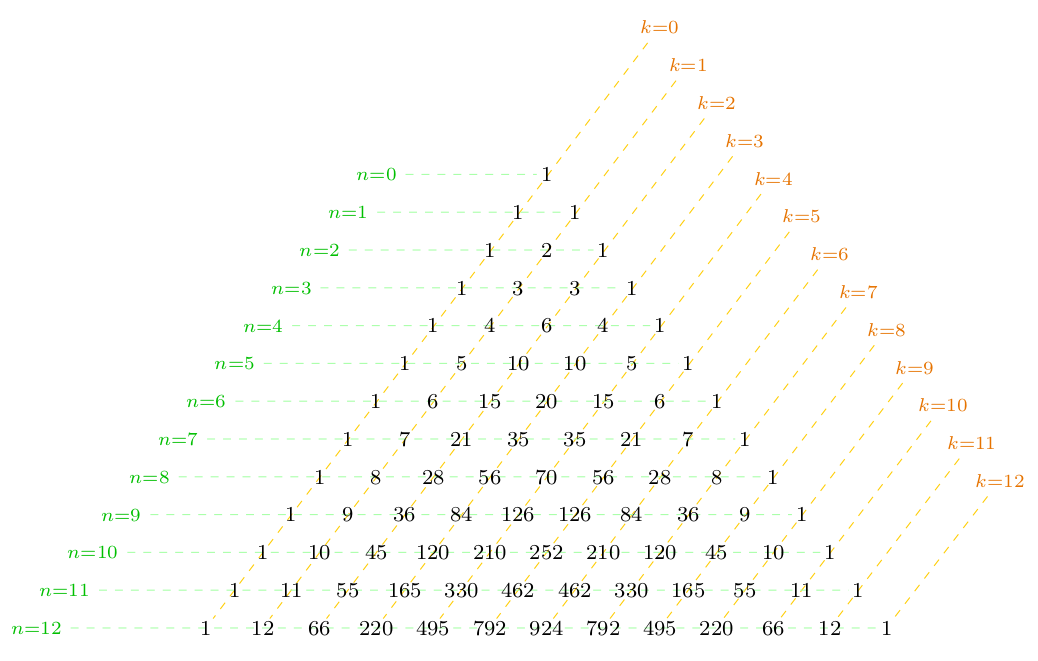
\includegraphics[scale=.5]{res/Tartaglia}
	\captionof{figure}{Triangolo di Tartaglia}\label{fig:tartaglia}
\end{center}

\section{Il principio di induzione}\label{sez:induzione}\index{Induzione}

\begin{propbox}[Principio di induzione (Prima forma)]
	Sia $p$ un predicato unario nella variabile $n$ e $b \in \mathbb{N}$ un numero naturale. Sia $\mathbb{N}_{b}=\{n \in \mathbb{N} \; | \; b \leq n \}$. Vale allora la seguente implicazione:
	\begin{equation}
		\Biggl(p(b) \land \Bigl(\forall n \in \mathbb{N}_{b}\bigl(p(n)\implies p(n+1) \bigr)\Bigr)\Biggr) \implies \forall n \in \mathbb{N}_{b} \bigl(p(n)\bigr)
	\end{equation}
	
\end{propbox}

\begin{proof}
	Si veda la sezione \ref{sez:buonordine}. 
\end{proof}

\begin{teorbox}
	Per ogni $n,k \in \mathbb{N}$ tali che $k \leq n$, vale allora:
	\begin{equation}
		\binom{n}{k} = \frac{n!}{k!(n-k)!}
	\end{equation}
\end{teorbox}

\begin{proof}
	Si dimostra per induzione.
	\begin{itemize}
		\item \textbf{Passo base:} sia $n=0$. Verifichiamo che il predicato sia vero. Se $n=0$ allora l'unico $k\leq n$ risulta essere $k=0$. Essendo $\binom{0}{0}=1$ allora  risulta :
		\begin{displaymath}
			\binom{0}{0} = \frac{0!}{0!} = 1
		\end{displaymath}
		e il predicato risulta vero. In generale:
		\begin{displaymath}
			\binom{n}{0} = \frac{n!}{0!(n-0)!} = \frac{n!}{n!} = 1
		\end{displaymath}
		\item \textbf{Passo induttivo:} assumiamo vero il predicato $p(n)$, dimostriamo $p(n) \implies p(n+1)$. Si ha:
		\begin{displaymath}
			\binom{n+1}{k} = \frac{(n+1)!}{k!(n+1-k)!}
		\end{displaymath}
		Se $k=0$ abbiamo che il predicato risulta vero. Se $k \neq 0$ applichiamo la formula \ref{eq:binom}:
		\begin{align*}
			\binom{n+1}{k} &= \binom{n}{k} + \binom{n}{k-1}\\
			&= \frac{n!}{k!(n-k)!} + \frac{n!}{(k-1)!(n-k+1)!}\\
			&= \frac{n!}{(k-1)!(n-k)!} \bigl(\frac{1}{k}+ \frac{1}{n-k+1}\bigr)\\
			&= \frac{n!}{(k-1)!(n-k)!} \bigl(\frac{n-k+1 +k}{k(n-k+1)}\bigr) \\
			&= \frac{n!(n+1)}{k!(n-k+1)!}\\
			&= \frac{(n+1)!}{k!\bigl((n+1)-k\bigr)!}
		\end{align*}
	\end{itemize}
	Il che dimostra il predicato $p(n+1)$.
\end{proof}
\newpage
\section{Esercizi svolti}
\begin{exsbox}
	Siano $X = \{1,2,3,4,5\}$ ed $Y=\{1,2,3\}$.
	\begin{enumerate}
		\item Quanti sono i sottoinsiemi di $X$ che contengono l'elemento 1?
		\item Quanti sono i sottoinsiemi $A$ di $X$ che contengono l'elemento 1 e tali che $A \cap \{2,3\} \neq \emptyset$?
		\item Quante sono le applicazioni iniettive da $X$ a $Y$?
		\item Quante sono le applicazioni iniettive da $Y$ a $X$?
		\item Quante sono le applicazioni suriettive da $X$ in $Y$?
	\end{enumerate}
\end{exsbox}
\paragraph{Svolgimento.} Abbiamo:
\begin{enumerate}
	\item Sia $\Omega$ l'insieme di tutti i sottoinsiemi di $X$ che contengono l'elemento $1$, ovvero:
	\begin{align*}
		\Omega \coloneqq \{A \subseteq X \; | \; 1 \in A\}
	\end{align*}
	Allora è immediato constatare che $\Omega$ è in corrispondenza biunivoca con l'insieme delle parti $X \setminus \{1\}$, mediante l'applicazione:
	\begin{align*}
		\varphi : \Omega \rightarrow \mathcal{P}(X \setminus \{1\})\\
		A \mapsto A \setminus \{1\}
	\end{align*}
	Ne segue che $|\Omega|= |\mathcal{P}(X \setminus \{1\})| = 2^{|X \setminus \{1\}|} = 2^{4} = 16$.
	\item Indichiamo con $\Theta$ il seguente insieme:
	\begin{align*}
		\Theta \coloneqq \{A \subseteq X \; | \; 1 \in A \land A \cap \{2,3\} \neq \emptyset \}
	\end{align*}
	Osserviamo che $\Theta$ è l'unione insiemistica di $\Lambda$ e $\Delta$, dove:
	\begin{align*}
		\Lambda \coloneqq \{ A \subseteq X \; | \; 1 \in A \land 2 \in A \}\\
		\Delta \coloneqq \{A \subseteq X \; | \; 1 \in A \land 3 \in A \}
	\end{align*}
	Pertanto $\Theta = \Lambda \cup \Delta$. Ragionando come nel punto precedente, si ha che:
	\begin{align*}
		|\Lambda|=|\Delta|= 2^{3} = 8
	\end{align*}
	Inoltre $\Lambda \cap \Delta \coloneqq \{A \subseteq X \; | \; \{1,2,3\} \subseteq A\}$, quindi $|\Lambda \cap \Delta|=2^{2}=4$. Siamo perciò in grado di calcolare con esattezza il numero di elementi di $\Theta$ tramite la \ref{eq:pie}:
	\begin{align*}
		|\Theta| = |\Lambda \cup \Delta| = |\Lambda|+|\Delta|-|\Lambda \cap \Delta| =12
	\end{align*}
	\item Essendo $|X| \geq |Y|$ non esistono applicazioni iniettive da $X$ in $Y$.
	\item Si ha $|Inj \ Map(Y,X)| = 5^{\underline{3}} = 5 \cdot 4 \cdot 3 = 60$ applicazioni iniettive.
	\item Sia $S \subseteq Map(X,Y)$ l'insieme di tutte le applicazioni suriettive da $X$ in $Y$. Inoltre, per ogni $y \in Y$ indichiamo con $A_{y}$ il sottoinsieme di $Map(X,Y)$ definito come:
	\begin{align*}
		A_{y} &\coloneqq \{f \in Map(X,Y) \; | \; y \notin f(X) \}\\
		&\coloneqq \{f \in Map(X,Y) \; | \; f^{-1}(\{y\}) = \emptyset\}
	\end{align*}
	Una applicazione $f$ è suriettiva se e solo se non appartiene a nessun $A_{y}$, per ogni $y=1,2,3$ abbiamo che:
	\begin{align}
		S = Map(X,Y) \setminus (A_{1} \cup A_{2} \cup A_{3})
	\end{align}
	Ne segue che:
	\begin{align*}
		|S| &=  |Map(X,Y)| - |A_{1} \cup A_{2} \cup A_{3}|\\
		&= 3^{5} - |A_{1} \cup A_{2} \cup A_{3}|
	\end{align*}
	Osserviamo che per ogni $f \in A_{1}$ vale $f(X) \subseteq \{2,3\}$, pertanto per tali funzioni l'insieme dei valori ammissibili è $\{2,3\}$, detto in altri termini: $|A_{1}| = |\{2,3\}|^{|X|} = 2^{5}$. Similmente per $A_{2}$ e $A_{3}$. Ora ci si accorge subito che $A_{1} \cap A_{2}$ contiene solo la funzione costante $c_{3}: x \mapsto 3$, per ogni $x \in X$ e, similmente, $A_{1} \cap A_{3} = \{c_{2}\}$, $A_{2} \cap A_{3} = \{c_{1}\}$. In particolare $|A_{1} \cap A_{2}|=|A_{1} \cap A_{3}| = |A_{2} \cap A_{3}| = 1$. Mentre $A_{1} \cap A_{2} \cap A_{3} = \emptyset$. Applicando la \ref{eq:pie2} otteniamo:
	\begin{align*}
		|A_{1} \cup A_{2} \cup A_{3}| &= |A_{1}|+|A_{2}| + |A_{3}| + |A_{1}\cap A_{2} \cap A_{3}| - |A_{1} \cap A_{2}| - |A_{1} \cap A_{3}| - |A_{2} \cap A_{3}| \\
		&= 3 \cdot 2^{5} + 3 \cdot 1 -0\\
		&= 3 \cdot (2^{5}-1)\\
		&= 3 \cdot 31
	\end{align*}
	Ne segue che $|S| = 150$. \hfill \blacksquare
\end{enumerate}
\begin{exsbox}
	Siano $A=\{n \in \mathbb{N} \ | \ n < 8\}$ e $B=\{n \in \mathbb{N} \ | \ n < 10 \}$. Esprimere:
	\begin{enumerate}
		\item $|A|$, $|B|$ e $|A \times B|$;
		\item il numero delle applicazioni da $A$ a $B$ e, tra queste, il numero di quelli iniettive, il numero di quelle suriettive, il numero di quelle biettive;
		\item il numero delle applicazioni da $A \times B$ a $B \times A$ e, tra queste, il numero di quelli iniettive, il numero di quelle suriettive, il numero di quelle biettive;
		\item il numero delle applicazioni costanti da $B$ ad $A$;
		\item il numero delle applicazioni f da B ad A tali che $f(0)=2$;
		\item il numero delle applicazioni f da B ad A tali che $im \ f \subseteq \{0,1,7\}$;
		\item il numero di applicazioni iniettive $f$ da $A$ a $B$ tali che $f(0) \neq 5$.
	\end{enumerate}
	Sia $X$ una parte di $A$. Supponiamo che esista un'applicazione suriettiva da $X$ ad $A$. Cosa sappiamo dire su $X$?
\end{exsbox}
\paragraph*{Svolgimento.} Si ha:
\begin{enumerate}
	\item $|A|=8$, $|B|=10$ e $|A \times B|=80$.
	\item Il numero di applicazioni da $A$ in $B$ è $|Map(A,B)| = 10^{8}$ mentre il numero di applicazioni iniettive da $A$ in $B$ è: $|Inj \ Map(A,B)| = 10^{\underline{8}}$. Non esistono applicazioni suriettive da $A$ in $B$ in quanto $|A| \leq |B|$ e di conseguenza non esistono applicazioni biettive da $A$ e $B$, non a caso $A$ e $B$ non possono essere equipotenti.
	\item Si ha che $|A \times B|=|B \times A|= 80$ e i due prodotti cartesiani sono quindi equipotenti. Il numero di applicazioni è dato da: $|Map(A \times B , B \times A)|=80^{80}$ mentre il numero di applicazioni iniettive e quindi biettive è $|Inj \ Map (A\times B, B \times A)|=80!$.
	\item Il numero di applicazioni costanti da $B$ in $A$ è dato dal numero degli elementi del codominio, ovvero $8$.
	\item Per trovare il numero di applicazioni $f$ da $B$ ad $A$ tali che $f(0)=2$ basta fissare tale mappa e considerare in numero di applicazioni tra il sottoinsieme $B \setminus\{0\}$ e $A$ ovvero: $|Map(B \setminus \{0\}, A)|= 8^{9}=8^{10}/8$
	\item Una funzione $f:B \rightarrow A$ tali che $im \ f \subseteq \{0,1,7\}$ può essere vista come una funzione $f: B \rightarrow \{0,1,7\}$ quindi il numero di applicazioni tra questi due insiemi è dato da $3^{10}$.
	\item Per trovare il numero di applicazioni iniettive da $A$ in $B$ tali che $f(0) \neq 5$ si ragiona nel modo seguente. All'elemento $0$ non è possibile associare l'elemento $5 \in B$, esisteranno quindi 9 possibili scelte diverse da poter assegnare:
	\begin{displaymath}
		0 \mapsto \underbrace{\cdots}_{\mbox{9 scelte}}
	\end{displaymath}
	All'elemento 1 sarà possibile assegnare $10-1$ scelte per ottenere una funzione iniettiva e così via:
	\begin{displaymath}
		\begin{array}{c}
			1 \mapsto \underbrace{\cdots}_{\mbox{9 scelte}} \\
			2 \mapsto \underbrace{\cdots}_{\mbox{8 scelte}} \\
			\vdots \\
			7 \mapsto \underbrace{\cdots}_{\mbox{3 scelte}}
		\end{array}
	\end{displaymath}
	Di conseguenza il numero di applicazioni iniettive tali che $f(0) \neq 5$ è dato da: $9 \cdot 9^{\underline{7}} = 9 \cdot 9 \cdot 8 \cdot 7 = 4536$.
\end{enumerate}
Se $X$ è una parte di $A$ ed esiste una applicazione suriettiva da $X$ in $A$ allora $A=X$. Infatti, dire che esiste una applicazione suriettiva da $X$ in $A$ significa affermare che $|X| \geq |A|$ ma questo è possibile se e solo se $|A|=|X|$ essendo $X$ una parte di $A$. \hfill \blacksquare
\begin{exsbox}
	Utilizzando un alfabeto $A$ di 7 caratteri, quante stringhe di lunghezza $n$ possiamo formare se $n=5$ e quante se $n=12$? E, in ciascuno dei due casi, quante senza ripetizioni di caratteri?
\end{exsbox}
\paragraph*{Svolgimento.} Utilizzando un alfabeto $A$ di 7 caratteri possiamo considerare l'applicazione:
\begin{displaymath}
	\lambda : I_{n} \longrightarrow A
\end{displaymath}
che associa ad ogni numero $m \in I_{n}$ un elemento di $A$ per costruire una stringa di lunghezza $n$. Dato $n=5$ allora $|Map(I_{n},A)|=7^{5}$. Se $n=12$ allora $|Map(I_{n},A)|=7^{12}$. Nel caso in cui $n=5$ si ha: $|Inj \ Map(I_{n},A)|=7^{\underline{5}}=2520$ mentre se $n=12$ non esistono applicazioni iniettive. \hfill \blacksquare
\begin{exsbox}
	Siano $S=\{0,1,5\}$ e $T=\{1,2\}$. Descrivere esplicitamente tutte le applicazioni iniettive da $T$ ad $S$ e le applicazioni suriettive da $S$ a $T$ (suggerimento per la seconda parte: si fa prima a dire quali non sono suriettive). Quante sono?
\end{exsbox}
\paragraph*{Svolgimento.} Dati gli insiemi $S=\{0,1,5\}$ e $T=\{1,2\}$ si hanno 6 funzioni iniettive da $T$ in $S$:
\begin{center}
	\begin{tblr}
		{hlines,
			vlines,
			colspec={cccccccccc},
			row{1}={primary!80!white},
			cells={mode=math},
			column{1}={primary!80!white},
			cell{2}{5}={yellow!7},
			cell{3}{5}={yellow!7},
			cell{2}{6}={yellow!7},
			cell{3}{6}={yellow!7},
			cell{2}{7}={yellow!7},
			cell{3}{7}={yellow!7},
			cell{2}{8}={yellow!7},
			cell{3}{8}={yellow!7},
			cell{2}{9}={yellow!7},
			cell{3}{9}={yellow!7},
			cell{2}{10}={yellow!7},
			cell{3}{10}={yellow!7}
		}
		t_{i} & c_{0} & c_{1} & c_{5} & f_{1} & f_{2} & f_{3} & f_{4} & f_{6} & f_{7} \\
		1 & 0 & 1 & 5 & 0 &0 &1 &1 & 5 &5\\
		2 & 0 & 1 & 5 & 1 &5 &0 &5 & 0 & 1\\
	\end{tblr}
\end{center}
Le funzioni $f_{1:7}$ sono tutte iniettive. Le applicazioni suriettive da $S$ in $T$ sono tutte quelle non costanti. \hfill \blacksquare

\begin{exsbox}
	Provare che se due insiemi $A$ e $B$ sono equipotenti, gli insiemi $(\mathcal{P}(A),\subseteq)$ e $(\mathcal{P}(B),\subseteq)$ sono isomorfi.
\end{exsbox}

\gbox{Numero di partizioni in un insieme finito}{red}{
	Indichiamo con $B_{n+1}$ il \textit{numero di partizioni di un insieme finito con $n$ elementi}. Si dimostra che un insieme con $n+1$ elementi ammette un numero di partizioni dato da:
	\begin{equation}
		B_{n+1} = \sum_{k=0}^{n} \binom{n}{k} B_{k}
	\end{equation}
In altri termini, il numero di partizioni di un qualsiasi insieme finito si può calcolare mediante la successione ricorsiva $\{B_{n}\}_{n \in \mathbb{N}}$ detta \textbf{successione dei numeri di Bell}\index{Numero di Bell}. I primi sette termini di tale successione sono:
$B_{0}=1$, $B_{1}=1$, $B_{2}=2$, $B_{3}=5$, $B_{4}=15$, $B_{5}=52$, $B_{6}=203$.
}
%  % Chapter 5: Strutture albegriche
  \chapter{Operazioni e strutture algebriche}
\section{Generalità sulle operazioni}

\begin{defbox}{Operazioni binarie}\index{Operazione!Binaria}
	Se $S$ è un insieme non vuoto, un'applicazione
	\begin{displaymath}
		\bot: S \times S \longrightarrow S
	\end{displaymath}
	si chiama \textbf{operazione binaria} (ovunque definita) in $S$. Qualunque siano gli elementi $x$ e $y$ di $S$,	l'immagine $\bot(x,y)$ della coppia $x,y$ mediante $\bot$ si dice \textbf{composto} di $x$ e $y$, e si denota col simbolo $x \bot y$.
\end{defbox}

\begin{example}
	\begin{enumerate}
		\item In $\mathbb{Z}$ sono operazioni binarie le operazioni di addizione, sottrazione e moltiplicazione.
	
		\item La divisione non è un'operazione binaria in $\mathbb{Z}$ in quanto non tutte le coppie $(m,n) \in \mathbb{Z}^{2}$ godono di composto. Ad esempio $(2,4)$, infatti: $2 \divslash 4 \notin \mathbb{Z}$.
	
		\item Fissato un insieme $A$ è possibile considerare l'insieme delle parti $\mathcal{P}(A)$. In $\mathcal{P}(A)$ è possibile considerare come operazioni binarie tutte le operazioni di intersezione, unione, differenza simmetrica e differenza, ecc.
	\end{enumerate}
\end{example}

Esiste un modo per rappresentare in tabella un'operazione. Supponiamo che l'insieme $S$ sia composto da tre elementi: $$S =\{a,b,c\}$$ Consideriamo un'operazione $\bot : S \times S \rightarrow S$ che può essere rappresentata mediante una tabella come mostrato qui di seguito:
\begin{center}
	\begin{tblr}{hlines,vlines,row{1}={primary!40!white},column{1}={primary!40!white},cells={mode=math},colspec={cccc}}
		\bot & a & b & c \\
		a & a \bot a & a \bot b & a \bot c \\
		b & b \bot a & b \bot b & b \bot c \\
		c & c \bot a & c \bot b & c \bot c \\
	\end{tblr}
\end{center}

Queste tabelle prendono il nome di \textbf{tavole di Cayley}.\index{Cayley}

\subsection{Proprietà delle operazioni}

\begin{defbox}{Operazioni associative}
	Sia $S$ un insieme non vuoto. Un'operazione $\bot: S \times S \longrightarrow S$ si dice \textbf{associativa} se risulta:
	\begin{displaymath}
		\forall x,y,z \in S \bigl( (x \: \bot \: y)\: \bot \: z = x \: \bot \: (y \:  \bot \: z)\bigr)
	\end{displaymath}
\end{defbox}


\begin{example}
	Sono un esempio di operazioni associative tutte le operazioni insiemistiche come l'unione, l'intersezione, la differenza simmetrica, l'unione unaria e l'intersezione unaria.
\end{example}

\begin{defbox}{Operazioni commutative}\index{Commutatività}
	Sia $S$ un insieme non vuoto. Un'operazione $\bot: S \times S \longrightarrow S$ si dice \textbf{commutativa} se risulta:
	\begin{displaymath}
		\forall x,y \in S \bigl(x \: \bot \: y = y \: \bot \: x\bigr)
	\end{displaymath}
	Due elementi $a,b$ di $S$ tali che $a \bot b = b \bot a$ si dicono \textbf{permutabili}.
\end{defbox}


\begin{osservation}
	È possibile determinare la proprietà commutativa di un'operazione osservando la relativa tavola di Cayley. Infatti, un'operazione gode della proprietà commutativa se e solo se la tavola di Cayley è \textit{simmetrica} lungo la propria diagonale.
\end{osservation}


\begin{example}
	Sia $s=\{a,b\}$, è possibile quindi considerare l'insieme $\mathcal{P}(s) = \{ \emptyset, \{a\}, \{b\}, s\}$ e l'operazione binaria interna $\cap : \mathcal{P}(s) \times \mathcal{P}(s) \rightarrow \mathcal{P}(s)$. Come ben sappiamo l'intersezione gode della proprietà commutativa e possiamo ben osservarlo costruendo la tavola di Cayley:
	\begin{center}
		\begin{tblr}
			{
				hlines,
				vlines,
				row{1}={primary!40!white},
				column{1}={primary!40!white},
				cells={mode=math},
				colspec={ccccc}
			}
			\cap & \emptyset & \{a\} & \{b\} & s \\
			\emptyset & \emptyset & \emptyset & \emptyset & \emptyset\\
			\{a\} & \emptyset & \{a\} & \emptyset & \{a\} \\
			\{b\} & \emptyset & \emptyset & \{b\} & \{b\} \\
			s & \emptyset & \{a\} & \{b\} & s
		\end{tblr}
	\end{center}
	\smallskip
	
	Infatti, osservando le celle dello stesso colore osserviamo che la tavola è simmetrica lungo la diagonale secondaria. Notiamo inoltre che, nonostante $\cap$ goda anche della proprietà associativa questa non può essere osservata dalla tavola ed è necessario quindi eseguire un controllo diretto tra tutte le possibili composte.
\end{example}

\begin{example}
	La sottrazione in $\mathbb{Z}$ non gode della proprietà commutativa e associativa. Infatti:
	\begin{displaymath}
		\forall a,b \in \mathbb{Z} \qquad a-b \neq b-a
	\end{displaymath}
	Infatti: $3-2\neq 2-3$.
	Per verificare l'associatività di una operazione è comodo verificare prima se essa gode della proprietà commutativa in quanto questa può velocizzare significativamente i calcoli. La sottrazione è associativa in $\mathbb{Z}$ se e solo se:
	\begin{displaymath}
		\forall a,b,c \in \mathbb{Z} \qquad \bigl( (a-(b-c)) = (a-b)-c \bigr)
	\end{displaymath}
	Per procedere avanti nella dimostrazione si osserva che: $a-(b-c)=(a-b)+c$. Quindi per essere associativa l'operazione deve valere:
	\begin{displaymath}
		(a-b)+c = (a-b)-c
	\end{displaymath}
	ma qualsiasi sia la terna, ad esempio $(0,0,1)$, si ha:
	\begin{displaymath}
		(0-0)+1\neq (0-0)-1
	\end{displaymath}
	Quindi l'operazione non è associativa in $\mathbb{Z}$.
\end{example}

\begin{teorbox}[Teorema di associatività]
	Se un'operazione $\star$ è associativa, presi $n$ elementi, qualsiasi sia l'ordine delle operazioni, il risultato è sempre lo stesso.
\end{teorbox}


\begin{teorbox}[Teorema di commutatività]
	Se un'operazione $\star$ è associativa e commutativa, dati $n$ elementi, qualsiasi sia l'ordine delle operazioni e degli operandi il risultato non cambia.
\end{teorbox}

\begin{example}
	L'associatività e la commutatività \textit{non sono correlate} tra di loro. Prendiamo ad esempio l'operazione binaria in $\mathbb{Z}$ definita come:
	\begin{displaymath}
		\forall a,b \in \mathbb{Z} \qquad a \ast b = (a+b)^{2}
	\end{displaymath}
	Questa operazione è banalmente commutativa in quanto:
	\begin{displaymath}
		\forall a,b \in \mathbb{Z} \qquad a \ast b = (a+b)^{2}=(b+a)^{2}=b \ast a
	\end{displaymath}
	ma non è associativa. Infatti, per essere associativa dovrebbe essere:
	\begin{displaymath}
		\forall a,b,c \in \mathbb{Z} \qquad a \ast (b \ast c) = (a \ast b) \ast c
	\end{displaymath}
	ma $$a \ast (b \ast c) = a \ast (b+c)^{2} = \bigl(a + (b+c)^{2}\bigr)^{2}$$
	e $$(a \ast b) \ast c = c \ast (a \ast b) = \bigl(c + (a+b)^{2}\bigr)^{2} $$
	sono diverse in quanto rappresentano due espressioni diverse qualunque sia la terna $(a,b,c)$.
\end{example}

\begin{defbox}{Operazioni distributive}\index{Distributività}
	Se $\bot$ e $\star$ sono operazioni in S, si dice che $\star$ è \textbf{distributiva a destra} rispetto a $\bot$ se per ogni terna $x,y,z$ di elementi di $S$ risulta
	\begin{equation}
		(x\: \bot \: y)\: \star \: z \;=\;(x \: \star z)\: \bot \: (y \: \star \: z)
	\end{equation}
Sarà \textbf{distributiva a sinistra} rispetto a $\bot$ se per ogni terna $x,y,z \in S$ risulta:
\begin{equation}
	x \ \star \ (y \ \bot \ z) = (x  \ \star \ y) \ \bot \ (x \ \star \ z) 
\end{equation}
Quando $\star$ è commutativa, allora le due condizioni sono equivalenti.
\end{defbox}

\begin{example}
\begin{enumerate}
	\item 	In $\mathbb{N}$ possiamo considerare le operazioni $\cdot$ e $+$ che corrispondono alle operazioni usuali di moltiplicazioni e addizione. Dalle proprietà dell'aritmetica sappiamo che vale la proprietà distributiva della moltiplicazione rispetto all'addizione:
	\begin{displaymath}
		\forall a,b,c \in \mathbb{N} \bigl(a \cdot (b+c) = a \cdot b + a \cdot c \bigr)
	\end{displaymath}
	\item L'unione insiemistica è distributiva rispetto all'intersezione, e l'intersezione è distributiva rispetto all'unione. Inoltre l'intersezione è distributiva rispetto alla differenza simmetrica.
\end{enumerate}
\end{example}

\begin{defbox}{Operazione opposta}\index{Operazione!Opposta}
	Sia $\ast: S \times S \longrightarrow S$ una operazione binaria in $S$. È possibile considerare l'\textbf{operazione opposta}\index{Operazione opposta} $\ast^{\ast}$ definita ponendo:
	\begin{equation}
		\forall a,b \in S (a \ast^{\ast}b=b \ast a)
	\end{equation}
	
\end{defbox}
L'operazione opposta ha le stesse proprietà dell'operazione iniziale. Riferendosi alla rappresentazione grafica delle tavole di Cayley, calcolare l'operazione opposta significa ribaltare la tavola rispetto a righe e colonne. 

\begin{osservation}
	Una operazione è commutativa se e solo se essa coincide con la propria operazione opposta.
\end{osservation}

\section{Strutture algebriche}
\subsection{Semigruppi}\index{Semigruppi}

\begin{defbox}{Struttura algebrica}\index{Struttura algebrica}
	Sia $S$ un insieme non vuoto e siano $\bot_{1},...,\bot_{n}$ $n$ operazioni in S. La $n+1$-pla $(S,\bot_{1},...,\bot_{n})$ si chiama \textbf{struttura algebrica} e l'insieme $S$ si chiama \textbf{sostegno} di tale struttura.
\end{defbox}

\begin{defbox}{Semigruppo}
	Una struttura algebrica ad una operazione interna $(S, \bot)$ si dice \textbf{semigruppo} se l'operazione $\bot$ è associativa. Un semigruppo $(S,\bot)$ si dice \textbf{commutativo} o \textbf{abeliano} se l'operazione $\bot$ è anche commutativa.
\end{defbox}

\begin{example}
\begin{enumerate}
	\item Gli insiemi $\mathbb{N},\mathbb{Z},\mathbb{Q},\mathbb{R}$ con l'usuale operazione somma sono tutti semigruppi. Analogamente se invece della somma consideriamo il prodotto.

	\item Sia $A$ un insieme, sia $A^{A}$ l'insieme delle funzioni $f:A \rightarrow A$ e sia $\circ$ la composizione di funzioni. Possiamo considerare la composizione come un'operazione su $A^{A}$:
	\begin{displaymath}
		\circ : (f,g) \in A^{A} \times A^{A} \mapsto f \circ g \in A^{A}
	\end{displaymath}
	Dato che $\circ$ è associativa la struttura $(A^{A},\circ)$ è un semigruppo.
	\item Consideriamo $\mathbb{Z}$ e la funzione $-: \mathbb{Z} \times \mathbb{Z}: (a,b) \mapsto a-b$. La funzione $-$ è un'operazione, ma non è associativa. Infatti è possibile trovare almeno una terna $a,b,c \in \mathbb{Z}$ per cui $a-(b-c)\neq (a-b)-c$. Per esempio $a=4$, $b=-2$, $c=8$:
	\[(4-(-2))-8=-2 \neq 10=4-(-2-8)\]
	Quindi l'operazione $-$ non dà su $\mathbb{Z}$ la struttura di semigruppo.
	\item Su $\mathbb{R} \times \mathbb{R}$ definiamo $(a,b) \ast (c,d)=(ac,ad+b)$. $(\mathbb{R}\times \mathbb{R},\ast)$ è un semigruppo. Infatti:
	\begin{align*}
		\forall (a,b),(c,d),(e,f) \in \mathbb{R}\times\mathbb{R}\Bigl((a,b)\ast \bigl((c,d) \ast (e,f)\bigr) &= (a,b) \ast (ce,cf+d) \\
		&= (ace, acf+ad+b) \\
		&= (ac,ad+b) \ast (e,f) \\
		&= \bigl((a,b)\ast(c,d)\bigr)\ast (e,f)\Bigr)
	\end{align*}
\end{enumerate}
\end{example}

\begin{defbox}{Parte stabile e operazione indotta}\index{Parte stabile}
	Sia $\bot: S \times S \longrightarrow S$ un'operazione nell'insieme non vuoto S. Una parte non vuota $X$ di $S$ si dice \textbf{stabile} o \textbf{chiusa} rispetto a $\bot$ se per ogni coppia $(x,y)$ di elementi di $X$ anche il composto $x\: \bot \: y$ appartiene a $X$. In questo caso l'applicazione
	\begin{displaymath}
		\bot_{X}\: : \:(x,y)\in X \times X \longmapsto x \: \bot \: y \in X
	\end{displaymath}
	è un'operazione in $X$, che si dice \textbf{indotta} da $\bot$ su $X$.
\end{defbox}

\begin{example}
	Consideriamo la struttura $(\mathbb{Z}, -)$, chiaramente $\mathbb{N} \subseteq \mathbb{Z}$ non è chiusa rispetto alla sottrazione.
\end{example}

\begin{defbox}{Sottostruttura algebrica}\index{Sottostruttura}
	Sia $(S,\bot_{1},...,\bot_{n})$ una struttura algebrica, e sia $X$ una parte non vuota di $S$ che sia stabile rispetto a ciascuna delle operazioni $\bot_{1},...,\bot_{n}$. La struttura algebrica $(X,\bot_{1},...,\bot_{n})$ si dice \textbf{sottostruttura} di $(S,\bot_{1},...,\bot_{n})$.
\end{defbox}

\begin{defbox}{Potenze in un semigruppo}
	Se $(S,\bot)$ è un semigruppo, possiamo definire le \textbf{potenze} di un elemento $a \in S$ mediante l'induzione:
	\begin{equation}
		\begin{cases*}
			a^{n} = a & \mbox{se } n=1 \\
			a^{n+1} = a^{n} \bot a & \mbox{se } n \geq 1
		\end{cases*}
	\end{equation} 
\end{defbox}

\begin{propbox}
	Sia $(S,\bot)$ un semigruppo. Se $a \in S$ e $m,n \in \mathbb{Z}^{+}$, allora:
	\begin{eqnarray}
		a^{n} \bot a^{m} &=& a^{n+m} \\
		(a^{n})^{m} &=& a^{nm}
	\end{eqnarray}
\end{propbox}
\begin{proof}
	Dimostriamo per induzione su $m$ che $a^{n} \bot a^{m} = a^{n+m}$. Se $m=1$, si ha $a^{n} \bot a^{1}=a^{n} \bot a = a^{n+1}$ per come abbiamo definito la potenza. Supponiamo che la proprietà sia vera per un certo $m$, ossia che valga $a^{n}\bot a^{m}= a^{n+m}$, e dimostriamo che allora vale la proprietà anche per l'intero successivo $m+1$, ossia che si ha $a^{n}\bot a^{m+1}=a^{n+m+1}$. Si hanno le uguaglianze:
	\begin{align*}
		a^{n} \bot a^{m+1} &= a^{n} \bot (a^{m}\bot a) & \text{\textcolor{gray}{(Per definizione di potenza)}} \\
		&= (a^{n} \bot a^{m}) \bot a & \text{\textcolor{gray}{(Per l'associatività di $\bot$)}}\\
		&= (a^{n+m}) \bot a & \text{\textcolor{gray}{(Per ipotesi induttiva)}}\\
		&= a^{n+m+1} & \text{\textcolor{gray}{(Per definizione di potenza)}}
	\end{align*}
Dimostriamo ora per induzione su $m$ che $(a^{n})^{m}=a^{nm}$. Per $m=1$, $(a^{n})^{1}=a^{n}=a^{n\cdot1}$. Supponiamo ora che sia vero che $(a^{n})^{m}=a^{nm}$ e otteniamo la catena di uguaglianze:
\begin{align*}
	(a^{n})^{m+1} &= (a^{n})^{m} \bot (a^{n})^{1} & \text{\textcolor{gray}{(Per definizione di potenza)}} \\
	&=(a^{n})^{m} \bot a^{n} & \text{\textcolor{gray}{(Per ipotesi induttiva)}} \\
	&= a^{nm} \bot a^{n} \\
	&= a^{nm+n} & \text{\textcolor{gray}{(Per la proprietà precedente)}}\\
	&= a^{n(m+1)} & \text{\textcolor{gray}{(Mettendo $n$ in evidenza)}}
\end{align*}
\end{proof}
Quando l'operazione che si considera è l'addizione tra elementi, il concetto di potenza si traduce nel concetto di \textit{multiplo}.

\begin{defbox}{Multiplo}\label{def:multiplo}\index{Multiplo}
	Sia $(S,+)$ un semigruppo denotato additivamente e sia $a \in S$. Qualsiasi sia $n \in \mathbb{N}^{+}$ si ha:
	\begin{equation}
		na = \underbrace{a + a + \ldots +a}_{\text{$n$ volte}}
	\end{equation}
	ed $na$ prende il nome di \textbf{multiplo} di $a$.
\end{defbox}

\subsection{I monoidi}\index{Monoide}

\begin{defbox}{Elemento neutro}\index{Elemento!Neutro}
	Sia $(S,\bot)$ una struttura algebrica ad una operazione interna. Un elemento $u$ di $S$ si chiama \textbf{elemento neutro a sinistra} se risulta
	\begin{equation}
		\forall x \in S\qquad u \ \bot \ x \ = \ x
	\end{equation}
	Si dice invece che u è \textbf{neutro a destra} se
	\begin{equation}
		\forall x \in S\qquad x \ \bot \ u \ = \ x
	\end{equation}
	$u$ è \textbf{elemento neutro} se è neutro sia a sinistra che a destra, cioè se risulta
	\begin{equation}
		\forall x \in S \qquad x\ \bot \ u \ = \ u \ \bot \ x \ = \ x
	\end{equation}
	La struttura $(S, \bot)$ si dice \textbf{unitaria} se è dotata di elemento neutro e si indica con $(S, \bot, u)$. Quando la struttura $(S, \bot)$ è commutativa le tre definizioni coincidono.
\end{defbox}

\begin{defbox}{Monoide}
	Sia S un insieme e $\bot$ un'operazione su S. Si dice che $(S, \bot)$ è un \textbf{monoide} se $\bot$ è associativa ed esiste l'elemento neutro. In altre parole un monoide $(S, \bot)$ è un semigruppo unitario. Spesso, per i monoidi, si usa la notazione $(S, \bot, u)$.
\end{defbox}


\begin{example}
\begin{enumerate}
	\item Gli insiemi $\mathbb{N},\ \mathbb{Z}, \ \mathbb{Q},\ \mathbb{R}$ con l'usuale operazione $+$ sono tutti monoidi, l'elemento neutro è sempre $0$. Analogamente se invece della somma consideriamo il prodotto, abbiamo struttura di monoide per tutti gli insiemi sopra citati, con elemento neutro $1$.

	\item Sia $Rel(a)$ l'insieme delle relazioni binarie nell'insieme $a$. Allora l'insieme $(Rel(a), \cdot , id_{a} )$ è un monoide, anche detto \textbf{monoide delle relazioni binarie} in $a$. Per quanto visto nell'Osservazione \ref{osservation:non_commutativity_composition}, il monoide non è abeliano in quanto il prodotto relazionale non è una operazione commutativa.
	\smallskip
	
	Inoltre, poiché la composizione di due relazioni binarie risulta ancora una relazione binaria, l'insieme $Map(a,a)$ delle applicazioni sull'insieme $a$, detto anche \textbf{insieme delle trasformazioni} e indicato anche con $T(a)$ o anche $a^{a}$, è una parte stabile del monoide delle relazioni binarie, in particolare ne è un \textbf{sottomonoide}\footnote{Il più importante monoide non commutativo.}.

	\item Consideriamo $\mathbb{Z}$ e l'operazione $\star$ definita ponendo:
	\begin{displaymath}
		a \star b \Coloneqq ab-a-b+2
	\end{displaymath}
	Verifichiamo se $(\mathbb{Z},\star)$ è un semigruppo. Prendo $a,b,c$ in $\mathbb{Z}$:
	\begin{eqnarray*}
		a \star ( b \star c)&=&a \star (bc-b-c+2)\\
		&=&(abc-ab-ac+2a)-a-(bc-b-c+2)+2\\
		&=& abc-ab-ac-bc+a+b+c \\
		(a\star b)\star c &=&(ab-a-b+2) \star c \\
		&=&(abc-ac-bc+2c)-(ab-a-b+2)-c+2\\
		&=&abc-ab-ac-bc+a+b+c
	\end{eqnarray*}
	Quindi $\star$ è associativa e $(\mathbb{Z},\star)$ è un semigruppo. Verifichiamo se esiste un elemento neutro $e$ rispetto all'operazione $\star$. Cerchiamo $e \in \mathbb{Z}$ tale che $e \star a =a \star e=a \qquad \forall a \in \mathbb{Z}$.
	\begin{equation*}
		a \star e = ae-a-e+2=a \Rightarrow (e-2)a+(e-2)=0 \Rightarrow e=2
	\end{equation*}
	L'elemento neutro esiste ed è $2$. Quindi $(\mathbb{Z},\star)$ è un monoide.

	\item Si consideri l'operazione di elevamento a potenza nell'insieme dei numeri reali munito dell'operazione di moltiplicazione:
	\begin{displaymath}
		\forall (a,b) \in \mathbb{R} \quad a^{b} =   \begin{cases}
			1 & \mbox{se } b=0 \\
			\underbrace{a \cdot a \cdot ... \cdot a}_{\text{$b$ volte}} & \mbox{se } b>0
		\end{cases}
	\end{displaymath}
	L'elemento $1 \in \mathbb{R}$ risulta neutro a destro in quanto $\forall a \in \mathbb{R}  (a^{1} = a)$, ma non neutro a sinistra dato che: $\forall a \in \mathbb{R} (1^{a} = 1)$.

	\item Si consideri l'insieme $s=\{a,b\}$ e il suo insieme delle parti $\mathcal{P}(s)=\{\varnothing,\{a\},\{b\},s\}$ già visto in precedenza. Chiaramente la struttura $(\mathcal{P}(a),\cap,a)$ è un monoide in quanto $\cap$ risulta essere una operazione associativa e $s$ risulta neutro rispetto a tale operazione. Infatti, per ogni $x \in \mathcal{P}(a)$ si ha $x \cap s = x$. La proprietà di essere elemento neutro è facilmente osservabile all'interno di una tavola di Cayley. Infatti, se un determinato elemento $t$ è elemento neutro a sinistra, allora la sua riga corrispondente conterrà l'intestazione della colonna corrispondente. Viceversa a destra.
	\medskip
	
	\begin{center}
		\begin{tblr}
			{
				vlines,
				hlines,
				row{1}={primary!40!white},
				column{1}={primary!40!white},
				colspec={ccccc},
				cells={mode=math},
				cell{2-5}{5}={yellow9},
				cell{5}{2-5}={yellow9}
			}
			\cap & \emptyset & \{a\} & \{b\} & s \\
			\emptyset & \emptyset & \emptyset & \emptyset & \emptyset\\
			\{a\} & \emptyset & \{a\} & \emptyset & \{a\} \\
			\{b\} & \emptyset & \emptyset & \{b\} & \{b\} \\
			s & \emptyset & \{a\} & \{b\} & s
		\end{tblr}
	\end{center}
\end{enumerate}
\end{example}

\begin{defbox}{Alfabeto}\index{Alfabeto}
	Sia $A$ un insieme, che chiamiamo \textbf{alfabeto}. Chiamiamo \textbf{parola nell'alfabeto} $A$ una qualsiasi sequenza $a_{1}a_{2}...a_{n}$ di elementi $a_{i} \in A$ (ed anche la parola vuota, sequenza di 0 simboli).
\end{defbox}

\begin{example}
	Sia $A = \{0,1,2,...,15\}$. Alcune parole nell'alfabeto $A$ sono ad esempio: ``$1 \ 5 \ 15$'', ``$4 \ 4 \ 4 \ 3 \ 4 \ 5$'', ``$6$''.
\end{example}

\begin{defbox}{Insieme delle parole}
	Per ogni $n \geq 0$, definiamo $W_{n}$ come l'insieme delle parole $w$ nell'alfabeto $A$ formate esattamente da $n$ elementi di A:
	\begin{equation}
		W_{n} \Coloneqq \{ w=a_{1}a_{2}...a_{n} \ | \ a_{i}\in A\}
	\end{equation}
	Per $n=0$, $W_{0}$ contiene un solo elemento, la \textbf{parola vuota} $w_{0}$ che non contiene nessun elemento di $A$. Invece $W_{1}=A$. L'insieme $W_{A}=\bigcup_{n \in \mathbb{N}}W_{n}$ è l'\textbf{insieme delle parole} dell'alfabeto $A$.
	
	Definiamo un'operazione su $W_{A}$: siano $w_{1}=a_{1}a_{2}...a_{n}$ e $w_{2}=b_{1}b_{2}...b_{m}$ due parole di $W_{A}$ e sia $$\circ \Coloneqq W_{A} \times W_{A} \longrightarrow W_{A}$$ definita ponendo:
	\begin{equation}
		w_{1} \circ w_{2} =a_{1}...a_{n}b_{1}...b_{m}
	\end{equation}
	$w_{1}\circ w_{2}$ è una parola di $W_{A}$ e $\circ$ è un'operazione, quindi $(W_{A},\circ)$ è una struttura algebrica. Chiamiamo $\circ$ operazione di \textbf{concatenazione}.
\end{defbox}

\begin{propbox}	
	$(W_{A},\circ)$ è un monoide.
\end{propbox}


\begin{proof}
	Dobbiamo dimostrare che $\circ$ è associativa ed esiste l'elemento neutro. Per l'associatività è sufficiente osservare che se $w_{1}=a_{1}...a_{n}$, $w_{2}=b_{1}...b_{m}$ e $w_{3}=c_{1}...c_{l}$ allora
	\begin{align*}
		(w_{1}\circ w_{2}) \circ w_{3} &= (a_{1} a_{2}...b_{1} b_{2}...b_{m})\circ w_{3}\\
		&= a_{1}a_{2}...a_{n}b_{1}b_{2}...b_{m}c_{1}c_{2}...c_{l}\\
		w_{1} \circ (w_{2} \circ w_{3}) &= w_{1} \circ (b_{1}b_{2}...b_{m}c_{1}c_{2}...c_{l})\\
		&= a_{1}a_{2}...a_{n}b_{1}b_{2}...b_{m}c_{1}c_{2}...c_{l}
	\end{align*}
	Inoltre l'elemento neutro rispetto a $\circ$ esiste, ed è la parola vuota $w_{0}$.
\end{proof}


\begin{osservation}
	Banalmente $\circ$ non è commutativo, quindi $(W_{A}, \circ, w_{0})$ è un esempio di monoide non commutativo.
\end{osservation}

\begin{teorbox}[Unicità dell'elemento neutro]\label{thm:neutro}
	Sia $(S, \bot)$ una struttura algebrica ad una operazione e siano $u$ un elemento neutro a sinistra di $S$ e $u'$ un elemento neutro a destra di $S$. Risulta allora $u=u'$. Inoltre, se $u$ è l'unico elemento neutro a sinistra in $(S, \bot)$ e l'unico elemento neutro a destra in $(S, \bot)$ allora sarà l'unico elemento neutro in $(S,\bot)$.
\end{teorbox}


\begin{proof}
	Poiché $u$ è neutro a sinistra ed $u'$ neutro a destra, si ha: $$u'=u \ \bot \ u' =u$$
	Per dimostrare che $u$ è unico consideriamo un elemento $t \in S$ neutro a sinistra rispetto a $\bot$. Allora, per la prima parte della dimostrazione si ha necessariamente: $t = u'$ e dunque: $t=u$. 
\end{proof}

\marker{yellow!50}{yellow!20!black}{Il teorema garantisce l'\emph{unicità dell'elemento neutro} (se questo esiste) ma non nega il fatto che \textit{possano esistere più di un elemento neutro a sinistra o a destra} (a condizione che nell'altro senso non ce ne siano).}

\begin{example}
	Si consideri ad esempio l'operazione:
\begin{displaymath}
	\ast : (a,b) \in S \times S \mapsto a \in S
\end{displaymath}
nota come \textbf{proiezione} in S della prima componente. La struttura $(S, \ast)$ è associativa. Infatti:
\begin{displaymath}
	\forall a,b,c \in S\qquad a \ast (b \ast c) = (a \ast b) \ast c
\end{displaymath}
In $(S, \ast)$ vale dunque la proprietà:
\begin{displaymath}
	\forall t \in S \quad (a \ast t) = a
\end{displaymath}
dunque $t$ è neutro a destra rispetto a $\ast$. Ogni elemento di $S$ risulta essere quindi un elemento neutro a destra.
\end{example}

\subsection{Elementi simmetrizzabili}

\begin{defbox}{Elemento simmetrico}\index{Elemento!Simmetrico}
	Sia $(S, \bot)$ una struttura algebrica dotata di elemento neutro u. Un elemento $x$ di $S$ si dice \textbf{simmetrizzabile a sinistra} se esiste $x'$ in $S$ tale che
	\begin{equation}
		x' \ \bot \ x = u
	\end{equation}
	e l'elemento $x'$ si chiama \textbf{simmetrico sinistro}. Analogamente, $x$ si dice \textbf{simmetrizzabile a destra} se esiste $x''$ di S tale che
	\begin{equation}
		x \ \bot \ x'' = u
	\end{equation}
	e in tal caso l'elemento $x''$ si chiama \textbf{simmetrico destro} di $x$.
	L'elemento $x$ si dice \textbf{simmetrizzabile} se esiste un elemento $x'$ di $S$ che sia simmetrico sinistro e destro di $x$, cioè tale che
	\begin{equation}
		x' \ \bot \ x= x \ \bot \ x' = u
	\end{equation}
	L'elemento $x'$ si dice allora un \textbf{simmetrico} di $x$. Ovviamente, se l'elemento $x$ è simmetrizzabile e $x'$ è un suo simmetrico, anche $x'$ è simmetrizzabile, e $x$ è un simmetrico di $x'$.
\end{defbox}

Se $(S, \bot)$ è un semigruppo dotato di elemento neutro e $x$ è un elemento simmetrizzabile di $S$, l'unico simmetrico di $x$ sarà denotato con $x'$. Se l'operazione nel semigruppo $S$ è denotata moltiplicativamente, un elemento simmetrizzabile di $S$ si dice \textbf{invertibile}, e il suo simmetrico si chiama \textbf{inverso} e si denota col simbolo $x^{-1}$. Se invece per l'operazione del semigruppo si usa la notazione additiva e $x$ è un elemento simmetrizzabile di $S$, il simmetrico di $x$ si chiama \textbf{opposto} e si denota col simbolo $-x$.

\begin{example}
	In $(\mathbb{Z}, \cdot)$ gli unici elementi ad avere simmetrico sono 1 e $-1$. Infatti $1 \cdot 1 = 1 = -1 \cdot (-1)$ e si dimostra che per ogni $a \in \mathbb{Z}\setminus\{\pm 1\}$ non esiste $a^{-1}$ tale che $a \cdot a^{-1} = 1$. In $(\mathbb{Z}, +)$ ogni elemento $n \in \mathbb{Z}$ ha simmetrico, che si indica con il simbolo $-n$.
\end{example}

\begin{defbox}{Insieme dei simmetrizzabili}
	Dato il monoide $(S, \bot, u)$, si denota con $\mathcal{U}$ l'\textbf{insieme degli elementi simmetrizzabili} di $S$ rispetto a $\bot$.
\end{defbox}

\begin{example}
	Ad esempio, se consideriamo il monoide dei numeri reali con l'operazione moltiplicazione si ha:
	\begin{displaymath}
		\mathcal{U}(\mathbb{R}, \times  , 1) = \mathbb{R} \setminus \{0\}
	\end{displaymath}
	mentre:	$\mathcal{U}(\mathcal{P}(A), \cup , \varnothing) = \{ \varnothing \}$ e $\mathcal{U}(\mathcal{P}(A), \cap, A) = \{A\}$.
\end{example}


\begin{propbox}
	Sia $(S,\bot,u)$ un monoide, e sia $x$ un elemento di $S$ per il quale esistano un simmetrico sinistro $x'$ e un simmetrico destro $x''$. Allora $x'=x''$ e quindi $x$ è simmetrizzabile. In particolare, un elemento simmetrizzabile di $S$ è dotato di un unico simmetrico.
\end{propbox}

\begin{proof}\label{key}
	Poiché l'operazione $\bot$ è associativa, risulta:
	\begin{displaymath}
		x'= x' \ \bot \ u = x' \ \bot \ (x \ \bot \ x'') = ( x' \ \bot \ x ) \ \bot \ x'' = u \ \bot \ x'' = x''
	\end{displaymath}
	il che dimostra l'enunciato.
\end{proof}


\begin{propbox}\label{prop:stabilitàsimmetrizzazione}
	Sia $(S,\bot,u)$ un monoide, e siano $x,y$ elementi simmetrizzabili di $S$. Allora $x \ \bot \ y$ è simmetrizzabile e risulta:
	\begin{equation}
		(x \ \bot \ y)' = y' \ \bot \ x'
	\end{equation}
\end{propbox}


\begin{proof}
	Si ha:
	\begin{displaymath}
		( x \ \bot \ y) \ \bot \ (y' \ \bot \ x') = x \ \bot \ (y \ \bot \ y') \ \bot \ x' = x \ \bot \ u \ \bot \ x' = x \ \bot \ x' = u
	\end{displaymath}
	e similmente $(y' \ \bot \ x') \ \bot \ (x \ \bot \ y ) = u$. Pertanto $x \ \bot \ y$ è simmetrizzabile, e $y' \ \bot \ \ x'$ è il suo simmetrico.
\end{proof}

\begin{osservation}
	Dalla Proposizione \ref{prop:stabilitàsimmetrizzazione} segue che, se $(S, \bot)$ è un semigruppo dotato di elemento neutro, l'insieme $\mathcal{U}(S)$ degli elementi simmetrizzabili di $S$ è una parte stabile.
\end{osservation}

In sintesi, un elemento $x \in (S,\bot, u)$ è:
\begin{center}
	\begin{tblr}{}
		Simmetrizzabile a sinistra & $\iff$ & $\exists x' \in S \bigl(x' \bot x = u \bigr)$ \\
		Simmetrizzabile a destra & $\iff$ & $\exists x' \in S \bigl(x \bot x' = u \bigr)$ \\
		Simmetrizzabile & $\iff$ & $\exists x' \in S \bigl(x \bot x' = x'  \bot x = u \bigr)$
	\end{tblr}
\end{center}

\subsection{Elementi cancellabili}
\begin{defbox}{Traslazioni}\index{Traslazione}
	Sia $(S,\bot)$ una struttura algebrica ad una operazione interna, e sia $a \in S$. È allora possibile considerare le applicazioni:
	\begin{displaymath}
		\sigma_{a}: x \in S \mapsto a \ \bot \ x \in S \qquad \text{e} \qquad \delta_{a}: x \in S \mapsto x\  \bot \ a \in S
	\end{displaymath}
	che si chiamano rispettivamente \textbf{traslazione sinistra} e \textbf{traslazione destra} di $S$ di \textbf{ampiezza} $a$.
\end{defbox}

\begin{defbox}{Elementi cancellabili}\index{Elemento!Cancellabile}
	Sia $(S, \bot)$ una struttura algebrica ad una operazione interna. Un elemento $a \in S$ si dice \textbf{cancellabile a sinistra} se vale
	\begin{equation}\label{eq:cancellabili_sx}
		\forall x,y \in S \bigl(	a \ \bot  \ x = a \ \bot \ y \Rightarrow x=y \bigr)
	\end{equation}
	ovvero se la traslazione sinistra  $\sigma_{a}$ è una applicazione iniettiva.
	
	Si dice che $a$ è \textbf{cancellabile a destra} se:
	\begin{equation}
		\forall x,y \in S \bigl(	x \ \bot \  a = y \ \bot \  a \Rightarrow x=y \bigr)
	\end{equation}
	Ovvero se la traslazione destra $\delta_{a}$ è una funzione iniettiva.	L'elemento si dice \textbf{regolare} o \textbf{cancellabile} se è cancellabile sia a sinistra che a destra, ovvero se entrambe le traslazioni $\sigma_{a}$ e $\delta_{a}$ risultano iniettive. 	$(S, \bot)$ si dice \textbf{regolare} se ogni suo elemento è regolare. In questo caso si dice anche che nella struttura algebrica $(S, \bot)$ vale la \textbf{legge di cancellazione}.
	
\end{defbox}

\begin{example}
	Rispetto all'operazione $+$ in $\mathbb{Z}$ tutti gli elementi sono cancellabili. Infatti, qualsiasi elemento $a \in \mathbb{Z}$ si ha:
	\begin{displaymath}
		\forall x, y \in \mathbb{Z} \bigl( a + x  = a + y \Rightarrow x=y \bigr)
	\end{displaymath}
\end{example}

\begin{example}
	In $(\mathbb{Z }, \cdot)$ tutti gli elementi sono cancellabili tranne il numero zero. Infatti un numero $a \in S$ non è cancellabile a sinistra in $(S, \ast)$ se e soltanto se esistono due elementi $x,y \in S$ tali che:
	\begin{displaymath}
		a \ \ast \ x = a \ \ast \ y \wedge x \neq y
	\end{displaymath}
	e nel caso di $0 \in \mathbb{Z}$ si ha ad esempio, presi due qualsiasi elementi $a,b$ diversi tra loro:
	\begin{displaymath}
		0 \cdot a = 0 = 0 \cdot b
	\end{displaymath}
	Quindi $0$ non è cancellabile.
\end{example}

Preso un insieme finito $A=\{1,2, \ldots, i,j, \ldots, n\}$ è possibile interpretare la cancellabilità in una struttura $(A,\bot)$ osservando la tavola di Cayley. Infatti, osservando la tabella \ref{tab:cayley} si può notare che ciascuna cella può essere vista come una traslazione sinistra dell'elemento della colonna determinata dall'elemento della riga corrispondente, oppure una traslazione destra dell'elemento della riga determinata dall'elemento della colonna corrispondente.

\begin{center}
	\begin{tblr}
		{
			hlines,
			vlines,
			row{1}={primary!40!white},
			column{1}={primary!40!white},
			cells={mode=math},
			colspec={ccccccccc}
		}
		\bot & 1 & 2 &  \cdots & i & j & \cdots & n\\
		1  & 1 \bot 1 & 1 \bot 2 &  \cdots & 1 \bot i & 1 \bot j & \cdots & 1 \bot n\\
		2 & 2 \bot 1 & 2 \bot 2 &  \cdots &  2 \bot i & 2 \bot j & \cdots & 2 \bot n\\
		\vdots & \cdots & \cdots &  \cdots & \cdots & \cdots & \cdots & \cdots \\
		i &  i \bot 1 & i \bot 2 &  \cdots &  i \bot i & \sigma_{i}(j)=i \bot j= \delta_{j}(i)& \cdots & i \bot n\\
		j &  j \bot 1 & j \bot 2 &  \cdots &  j \bot i & j \bot j & \cdots & j \bot n\\
		\vdots & \cdots & \cdots &  \cdots & \cdots & \cdots & \cdots & \cdots \\
		n & n \bot 1 & n \bot 2 &  \cdots &  n \bot i & n \bot j & \cdots & n \bot n\\
	\end{tblr}
	\captionof{table}{}\label{tab:cayley}
\end{center}

Quindi, se si notano ripetizioni sulla stessa riga, sia questa ad esempio quella dell'elemento $a$, vuol dire che l'applicazione $\sigma_{a}$ non è iniettiva e che l'elemento $a$ non è cancellabile a sinistra. Analogamente, se si notano ripetizioni sulla stessa colonna, sia questa ad esempio $a$, vorrà dire che l'applicazione $\delta_{a}$ non è iniettiva e che quindi l'elemento $a$ non è cancellabile a destra.

\begin{example}	
	Sia $A$ un insieme non vuoto e consideriamo la struttura algebrica $(\mathcal{P}(A),\setminus)$, dove con $\setminus$ si intende la differenza insiemistica. Quali sono gli elementi cancellabili a sinistra e a destra in questa struttura? Per definizione di elemento cancellabile a sinistra, un elemento $x \in \mathcal{P}(A)$ deve soddisfare alla seguente condizione:
	\begin{displaymath}
		\forall a,b \in \mathcal{P}(A) \bigl(x \setminus a = x \setminus b \Rightarrow a=b \bigr)
	\end{displaymath}
	È immediato osservare che la funzione:
	\begin{displaymath}
		x \in \mathcal{P}(A) \mapsto A \setminus x \in \mathcal{P}(A)
	\end{displaymath}
	è iniettiva. Infatti, se $A \setminus x = A \setminus b$, qualsiasi siano le parti $a,b$ di $A$ allora deve essere per forza $a=b$. Quindi l'insieme $A$ è cancellabile a sinistra. Analogamente, la funzione:
	\begin{displaymath}
		x \in \mathcal{P}(A) \mapsto x \setminus \varnothing \in \mathcal{P}(A)
	\end{displaymath}
	è chiaramente iniettiva e l'insieme vuoto risulta cancellabile a destra. Come si fa a dimostrare se ce ne sono altri di elementi cancellabili? $A$ ipoteticamente potrebbe essere infinito quindi risulta difficile verificare le proprietà di cancellabilità per ciascun elemento. Per questo motivo bisogna sfruttare le proprietà dei quantificatori. Infatti, negando ad esempio l'equazione \ref{eq:cancellabili_sx} si ottiene che un elemento $x \in \mathcal{P}(A)$ \textbf{non è cancellabile} se e soltanto se:
	\begin{displaymath}
		\exists b,c \in \mathcal{P}(A) \bigl( (x \setminus b = x \setminus c) \wedge (b \neq c) \bigr)
	\end{displaymath}
	La prova della cancellabilità di un elemento si riduce così nella ricerca di almeno un controesempio che soddisfa la formula appena descritta. Si ha infatti, ponendo: $b= \varnothing$ e  $c=A \setminus x$ si ottiene:
	\begin{displaymath}
		\begin{array}{l}
			x \setminus b = x \setminus \varnothing = x \\
			x \setminus c = x \setminus A \setminus x = x
		\end{array}
	\end{displaymath}
	Ma $b \neq c$ e quindi si ha che ogni parte $x \in \mathcal{P}(A)$ non è cancellabile a sinistra.
\end{example}


\begin{teorbox}[degli elementi cancellabili]\label{thm:cancellabili}
	Sia $(S,\bot,u)$ un monoide e sia $a \in S$. Valgono allora le seguenti implicazioni:
	\begin{enumerate}
		\item Se $a$ simmetrizzabile a sinistra rispetto a $\bot$ allora $a$ è cancellabile a sinistra rispetto a $\bot$;
		\item Se $a$ simmetrizzabile a destra rispetto a $\bot$ allora $a$ è cancellabile a destra rispetto a $\bot$;
		\item Se $a$ simmetrizzabile rispetto a $\bot$ allora $a$ è cancellabile rispetto a $\bot$;
	\end{enumerate}
\end{teorbox}

\begin{proof}
	Dimostriamo la prima implicazione. Siano quindi $x$ e $y$ elementi di $S$ tali che $$a \ \bot \ x = a \ \bot \ y$$ Si ha allora:
	\begin{align*}
		x &= u \ \bot \ x & \text{\textcolor{gray}{Per definizione di elemento neutro}} \\
		&= (a' \ \bot \ a) \ \bot x & \text{\textcolor{gray}{Per definizione di elemento simmetrizzabile}} \\
		&= a' \ \bot \ (a \ \bot \ x) & \text{\textcolor{gray}{Per associatività}} \\
		&= a' \ \bot \ (a \ \bot \ y) & \text{\textcolor{gray}{Per ipotesi}} \\
		&= (a' \ \bot \ a) \bot \ y  = u \ \bot \ y = y
	\end{align*}
	e quindi $a$ è cancellabile a sinistra. Un ragionamento analogo prova che $a$ è cancellabile a destra, e quindi cancellabile. 
\end{proof}

\marker{yellow!50}{yellow!20!black}{Attenzione, non vale il contrario. Un elemento può essere cancellabile ma non simmetrizzabile. Il viceversa \textbf{vale solo nei monoidi finiti}.}

\begin{example}
	Nel monoide infinito $(\mathbb{Z},\cdot,1)$ gli unici elementi simmetrizzabili sono $\pm 1$ ma 3 ad esempio è un elemento cancellabile.
\end{example}

In sintesi, un elemento $a \in (S,\bot, u)$ è:
\begin{center}
	\begin{tblr}
		{}
		Cancellabile a sinistra & $\iff$ & $\forall x,y \in S\bigl(a \bot x = a \bot y \implies x=y\bigr)$ \\
		Cancellabile a destra & $\iff$ & $\forall x,y \in S\bigl(x \bot a = y \bot a \implies x=y \bigr)$ \\
		Cancellabile & $\iff$ & è cancellabile sia destra che a sinistra.\\
		Simmetrizzabile & $\implies$ & Cancellabile
	\end{tblr}
\end{center}

\section{Gruppi}
\begin{defbox}{Gruppo}
	Siano $G$ un insieme e $\bot$ un'operazione in $G$. Diremo che $(G,\bot)$ è un \textbf{gruppo} se:
	\begin{enumerate}
		\item L'operazione $\bot$ è associativa: $\forall a,b,c \in G \bigl((a \bot (b \bot c) = (a \bot b) \bot c)\bigr)$;
		\item Esiste un elemento $e \in G$, detto \textbf{identità} o \textbf{elemento neutro} tale che $\forall x \in G (a \ \bot \ e = e \ \bot \ a = a)$;
		\item Ogni elemento ha l'inverso, ossia $
		\forall a \in G\bigl(\exists b \in G (a \ \bot \ b = b \ \bot \ a = e)\bigr)$.
	\end{enumerate}
	Un gruppo $(G, \bot)$ si dice \textbf{gruppo abeliano} se l'operazione $\bot$ è anche commutativa, assia $\forall a,b \in A $ si ha $a\  \bot \ b = b \ \bot \ a$.
\end{defbox}


\begin{osservation}
	Un gruppo altro non è che \emph{un monoide in cui ogni elemento è invertibile}.
\end{osservation}


Salvo avviso contrario, l'operazione in un gruppo sarà denotata \textit{moltiplicativamente}. In notazione moltiplicativa, l'elemento neutro di un gruppo viene denotato col simbolo 1 e detto \textbf{unità} di $G$, il simmetrico di un elemento $x \in G$ è chiamato \textbf{inverso} di $x$ e denotato col simbolo $x^{-1}$. In notazione additiva il simbolo per l'elemento neutro è $0$, se $(G,+)$ è un monoide commutativo, un elemento $a \in G$ è invertibile se esiste $b \in G$ tale che $a+b=0$, in tal caso si scrive $b=-a$ (invece di $b=a^{-1}$) e $-a$ si chiama \textbf{opposto} di $a$.

\begin{example}
\begin{enumerate}
	\item Il semigruppo $A^{A}$ delle trasformazioni $f:A \longrightarrow A$ non è un gruppo se $|A|\geq 2$, poiché ad esempio le funzioni costanti non hanno inverso. Se infatti $a,b \in A$ sono due elementi diversi e indichiamo con $c_{a}$ la funzione costante data da $\forall x \in A (c_{a}(x)= a)$, allora la composizione $c_{a} \circ g$ di una qualsiasi funzione $g \in T(A)$ con $c_{a}$, coincide con $c_{a}$ ed è quindi diversa da $id_{A}$: si ha ad esempio $c_{a}(b)= a \neq id_{A}(b)=b$.

	\item Si consideri il monoide $(\mathcal{P}(A), \triangle, \emptyset)$. Si ha:
	\begin{displaymath}
		\forall x \in \mathcal{P}(A) (x \triangle x = \emptyset)
	\end{displaymath}
	Quindi $x$ è il simmetrico di sé stesso. Quindi, se due insiemi $a,b \in \mathcal{P}(A)$ determinano $a \triangle b = \emptyset$ allora deve essere necessariamente $a=b$. In particolare $(\mathcal{P}(A), \triangle, \emptyset)$ è un gruppo.
\end{enumerate}
\end{example}

\begin{osservation}
	Se $(S, \bot)$ è un semigruppo dotato di elemento neutro e $\mathcal{U}(S)$ è l'insieme dei suoi elementi simmetrizzabili  allora $(\mathcal{U}, \bot)$ è un gruppo, chiamato \textbf{gruppo degli invertibili}.
\end{osservation}


\begin{defbox}{Potenza}
	Sia $G$ un gruppo e sia $g \in G$ e $n \in \mathbb{Z}$. La \textbf{potenza} $n$-esima $g^{n}$ di $g$ si definisce nella maniera seguente:
	\begin{equation}
		\begin{cases}
			\mbox{se } n=0 & g^{0} = 1_{G} \\
			\mbox{se } n>0 & g^{n} \ \mbox{è la potenza di $g$ che abbiamo definito nei semigruppi}\\
			\mbox{se } n<0 \mbox{ossia $n=-m$ con $m$ positivo }& g^{n} =(g^{-1})^{m}
		\end{cases}
	\end{equation}
\end{defbox}

Le proprietà delle potenze che abbiamo dimostrato nei semigruppi relativamente al caso degli esponenti positivi valgono nel caso dei gruppi anche per gli esponenti minori o uguali a 0 e si estendono a proprietà che riguardano gli inversi.

\begin{propbox}
	Sia $G$ un gruppo, $g \in G$ e siano $n,m \in \mathbb{Z}$. Allora:
	\begin{eqnarray}
		g^{n+m}=g^{n}g^{m} \\
		g^{nm}=(g^{n})^{m} \\
		(g^{m})^{-1} = g^{-m}
	\end{eqnarray}
\end{propbox}

\begin{propbox}
	Sia $G$ un gruppo denotato additivamente, $a \in G$ e siano $n,m \in \mathbb{Z}$. Allora:
	\begin{eqnarray}
		(n+m)a &= na+ma\\
		(nm)a &= n(ma)
	\end{eqnarray}
\end{propbox}


\begin{osservation}
	Nel gruppo abeliano $(\mathbb{Z},+)$ qualunque siano gli elementi $m,n$ il multiplo di $m$ secondo $n$ coincide con il multiplo di $n$ secondo $m$, ovvero il prodotto $nm$. L'\textbf{insieme dei multipli} di un elemento $n$ è denotato con il simbolo $n\mathbb{Z}$.
\end{osservation}


\subsection{Sottogruppi di un gruppo}
\begin{defbox}{Sottogruppo}
	Sia $(G, \bot)$ un gruppo e sia $H$ una parte stabile di $G$. $H$ si dice un \textbf{sottogruppo} di $G$ se la sottostruttura $(H, \bot)$ è un gruppo. Se $H$ è un sottogruppo di un gruppo $G$ si usa indicarlo con la notazione $H \leq G$.
\end{defbox}

\begin{example}
\begin{enumerate}
	\item Qualunque sia il gruppo $G$, i sottoinsiemi $G$ e $\{1\}$ sono evidentemente sottogruppi di $G$, chiamati \textbf{sottogruppi banali} di $G$. In particolare, $\{1\}$ si dice \textbf{sottogruppo identico} di $G$, mentre i sottogruppi di $G$ diversi da $G$ si dicono \textbf{sottogruppi propri} di $G$. È inoltre chiaro che, se $H$ è un sottogruppo di $G$, i sottogruppi di $H$ sono precisamente i sottogruppi di $G$ contenuti in $H$.

	\item L'insieme $\mathbb{Z}$ è un sottogruppo di $(\mathbb{Q},+)$, mentre $\{1,-1\}$ è un sottogruppo di $(\mathbb{Q}\setminus \{0\}, \cdot)$.
\end{enumerate}
\end{example}

\begin{lemmabox}
	Sia $G$ un gruppo, e sia $H$ un sottogruppo di $G$. Allora:
	\begin{enumerate}
		\item L'elemento neutro di $H$ coincide con l'unità di $G$
		\item Se $h$ è un elemento di $H$, il simmetrico di $h$ in $H$ coincide con l'inverso di $h$ in $G$.
	\end{enumerate}
\end{lemmabox}

\begin{proof}
	$(1)$ Se $u$ è l'elemento neutro di $H$, risulta $uu=u=u1$, e quindi $u=1$ per la legge di cancellazione in $G$.
	
	$(2)$ Sia $h'$ il simmetrico di $h$ in $H$. Poiché l'elemento neutro di $H$ è 1, si ha $h'h=1=h^{-1}h$ e quindi $h'=h^{-1}$. 
\end{proof}


\begin{corolbox}
	Sia $G$ un gruppo. Una parte $H$ di $G$ è un sottogruppo se e solo se è stabile, contiene l'unità di $G$ e l'inverso di ogni suo elemento.
\end{corolbox}

\begin{example}
	Consideriamo il gruppo abeliano $(\mathbb{Z},+)$. Un suo sottogruppo è l'insieme dei multipli di n in $\mathbb{Z}$, ossia l'insieme $n\mathbb{Z}=\{nk \; | \; k \in \mathbb{Z}\}$. Infatti, sommando due multipli di $n$ si otterrà sempre un multiplo di $n$, inoltre $0 \in n\mathbb{Z}$ e vale $-(nk) = n(-k) \in n \mathbb{Z}$.
\end{example}

\begin{teorbox}[caratterizzazione dei sottogruppi]
	Sia $G$ un gruppo. Una parte stabile non vuota $H$ di $G$ è un sottogruppo se e solo se per ogni coppia $(x,y)$ di elementi di $H$ anche il prodotto $x^{-1}y$ appartiene ad $H$.
\end{teorbox}


\begin{proof}
	Se $H$ è un sottogruppo di $G$, e $x$ e $y$ sono elementi di $H$, anche $x^{-1}$ appartiene ad $H$ e quindi, essendo $H$ stabile, si ha $x^{-1}y \in H$. Allo scopo di provare che la condizione dell'enunciato è anche sufficiente, sia $x$ un elemento della parte non vuota $H$ di $G$. Dall'ipotesi segue che $1=x^{-1}x$ appartiene ad $H$. Allora anche $x^{-1}=x^{-1}1$ appartiene ad $H$. Siano infine $x$ e $y$ elementi di $H$. Risulta $xy=(x^{-1})^{-1}y$, per cui $xy$ è in $H$, e $H$ è un sottogruppo di $G$. 
\end{proof}

\subsection{Parti chiuse e generatori}
\begin{propbox}
	Sia $(S,\bot)$ un semigruppo e sia $L$ un insieme di parti chiuse di $S$. Allora $\bigcap L$ è una parte chiusa di $S$.
\end{propbox}
\begin{proof}
	Si ha infatti:
	\begin{align*}
		\forall x,y \in \bigcap L \bigl( \forall X \in L ( x,y\in X \implies x \bot y \in X ) \bigr)
	\end{align*}
	Quindi se si prendono due elementi di $ \bigcap L$, anche il loro composto tramite $\bot$ appartiene a tutti gli elementi di $L$, ovvero $x \bot y \in \bigcap L$.
\end{proof}

\begin{defbox}{Sottostrutture generate}
	Data una struttura algebrica $(s,\bot)$ e $t \subseteq s$ una sua parte, definiamo:
	\begin{equation}
		\langle t \rangle  = \bigcap \{x \in \mathcal{P}(s) \; | \; t \subseteq x \land \text{$x$ è chiusa rispetto a $\bot$} \}
	\end{equation}
	Ovvero l'intersezione delle sottostrutture di $s$ che contengono $t$ e diciamo che $\langle t \rangle$ è la \textbf{sottostruttura generata} da $t$.
\end{defbox}

\begin{teorbox}[Caratterizzazione delle sottostrutture generate da singleton]
	Valgono le seguenti equivalenze:
	\begin{enumerate}
		\item Sia $(S,\bot)$ un semigruppo e $x \in S$, la parte chiusa generata da $\{x\}$ è $\langle \{x\} \rangle =\{x^{n} \; | \; n \in \mathbb{N}^* \}$;
		\item Sia $(S,\bot)$ un monoide e $x \in S$, la parte chiusa generata da $\{x\}$ è $\langle \{x\} \rangle = \{x^{n} \; | \; n \in \mathbb{N}\}$;
		\item Sia $(S,\bot)$ un gruppo e $x \in S$, la parte chiusa generata da $\{x\}$ è $\langle \{x\} \rangle  = \{x^{n} \; | \; n \in \mathbb{Z}\}$.
	\end{enumerate}
\end{teorbox}

\begin{osservation}
	La ragione per cui la chiamiamo ``generata'' è che si può dimostrare che essa è in realtà l’insieme delle combinazioni lineari dell’insieme $t$. Per esempio, il sottomonoide generata da  $\{2\} \subseteq (\mathbb{N}, +)$ è l’insieme di tutti i valori che si	possono ottenere sommando due: $$\langle2 \rangle= \{2, 4, 6, 8, 10, 12, 14, 16, 18, 20, \dots\}$$
\end{osservation}
\subsection{Il gruppo delle permutazioni}
\begin{defbox}{Gruppo simmetrico}\index{Gruppo simmetrico}
	Consideriamo il monoide $(T(A), \circ, id_{A})$, dove $T(A)$ è l'insieme delle trasformazioni in $A$. Chiaramente $(\mathcal{U}(T(A)), \circ)$ è un gruppo. I suoi elementi sono tutti e soli quelli del tipo:
\begin{displaymath}
	\mathcal{U}(T(A)) = \{ f \in T(A) \ | \ \exists g \in T(A) \bigl( f \circ g = g \circ f = id_{A} \bigr)\}
\end{displaymath}
ovvero tutte le applicazioni biettive in $T(A)$, chiamate anche \textbf{permutazioni} di $A$. Tale gruppo è denotato col simbolo $Sym(A)$ ed è chiamato \textbf{gruppo simmetrico}:
\begin{equation}
	Sym(A) = (\mathcal{U}\bigl(T(A)\bigr), \circ)
\end{equation}
Fissiamo un numero intero positivo $n$. Denotiamo con $I_{n}$ l'insieme dei numeri naturali $\{1,...,n\}$. L'insieme di tutte le permutazioni definite su $I_{n}$ si denota col simbolo $S_{n}$.
\end{defbox}

\begin{example}\label{example:permutazion1}
	Consideriamo in $S_{5}$ la permutazione $\sigma$ data da:
	\begin{displaymath}
		\sigma : I_{5} \longrightarrow I_{5}
	\end{displaymath}
	\begin{center}
		\begin{tikzpicture}[>=latex]
			\node(1){1};
			\node[right=0.3cm of 1](2){2};
			\node[right=0.3cm of 2](3){3};
			\node[right=0.3cm of 3](4){4};
			\node[right=0.3cm of 4](5){5};
			\node[below=1cm of 1](6){1};
			\node[right=0.3cm of 6](7){2};
			\node[right=0.3cm of 7](8){3};
			\node[right=0.3cm of 8](9){4};
			\node[right=0.3cm of 9](10){5};
			\draw[|->](1) -- (8);
			\draw[|->](2) -- (9);
			\draw[|->](3) -- (6);
			\draw[|->](4) -- (10);
			\draw[|->](5) -- (7);
		\end{tikzpicture}
	\end{center}
	Per scrivere in modo veloce $\sigma$ si usa una tabella costituita da due righe: nella prima sono elencati ordinatamente gli elementi di $I_{5}$ e al di sotto di ciascuno di essi, la seconda riga contiene le loro immagini. Otteniamo così la seguente tabella:
	\begin{displaymath}
		\sigma =
		\left(
		\begin{array}{lllll}
			1 & 2 & 3 & 4 & 5 \\
			3 & 4 & 1 & 5 & 2
		\end{array}
		\right)
	\end{displaymath}
\end{example}

Possiamo utilizzare una tabellina analoga a quella presentata nell'esempio per scrivere in modo sintetico qualsiasi permutazione. Nella prima riga elenchiamo gli elementi di $I_{n}$ e al di sotto di ciascuno scriviamo la sua immagine:
\begin{displaymath}
	\left(
	\begin{array}{ccccc}
		1 & 2 & \cdots & n-1 & n \\
		\sigma(1) & \sigma(2) & \cdots & \sigma(n-1) & \sigma(n)
	\end{array}
	\right)
\end{displaymath}
\begin{example}
	Sia $A=\{a,b\}$ con $a \neq b$, in questo caso $A^{A}$ avrà 4 elementi: $A^{A} = \{f \ | \ f: A \rightarrow A\}= \{id_{A}, c_{a}, c_{b}, \sigma \}$, con $\sigma : A \longrightarrow A$ che mappa $a$ in $b$ e $b$ in $a$. In questo caso l'insieme delle permutazioni di $A$ è:
	$$Sym(A)=\{id_{A},\sigma\}$$
\end{example}
\begin{example}
Consideriamo in $S_{5}$ la permutazione $\sigma$ dell'esempio \ref{example:permutazion1} e la seguente permutazione $\tau$:
	\begin{displaymath}
		\tau =
		\left(
		\begin{array}{lllll}
			1 & 2 & 3 & 4 & 5 \\
			1 & 3 & 4 & 5 & 2
		\end{array}
		\right)
	\end{displaymath}
	Possiamo comporre $\sigma$ e $\tau$. Poiché la composizione di funzioni non è commutativa, eseguiamo entrambe le composizioni (ottenendo risultati diversi):
	\begin{displaymath}
		\begin{array}{l}
			(\sigma \circ \tau)(1)=\sigma(\tau(1))=\sigma(1)=3 \\
			(\sigma \circ \tau)(2)=\sigma(\tau(2))=\sigma(3)=1 \\
			(\sigma \circ \tau)(3)=\sigma(\tau(3))=\sigma(4)=5 \\
			(\sigma \circ \tau)(4)=\sigma(\tau(4))=\sigma(5)=2 \\
			(\sigma \circ \tau)(5)=\sigma(\tau(5))=\sigma(2)=4
		\end{array}
	\end{displaymath}
	Riassumendo con la scrittura tabellare:
	\begin{displaymath}
		\sigma \circ \tau =
		\left(
		\begin{array}{lllll}
			1 & 2 & 3 & 4 & 5 \\
			3 & 1 & 5 & 2 & 4
		\end{array}
		\right)
	\end{displaymath}
	Analogamente, possiamo calcolare $\tau \circ \sigma$, ottenendo:
	\begin{displaymath}
		\tau \circ \sigma =
		\left(
		\begin{array}{lllll}
			1 & 2 & 3 & 4 & 5 \\
			4 & 5 & 1 & 2 & 3
		\end{array}
		\right)
	\end{displaymath}
\end{example}

\begin{defbox}{$K$-cicli e trasposizioni}
	Sia $k$ un numero intero tale che $1\leq k \leq n$. Si dice che una permutazione $f \in S_{n}$ è un \textbf{$k$-ciclo}, oppure un \textbf{ciclo di lunghezza $k$} se esistono elementi a due a due distinti $i_{1},\ldots,i_{k} \in I_{n}$ tali che:
	\begin{displaymath}
		\begin{array}{lllll}
			f(i_{1})=i_{2}, & f(i_{2})=i_{3}, & \ldots ,& f(i_{k-1})=i_{k}, & f(i_{k})=i_{1}
		\end{array}
	\end{displaymath}
	e $f(j)=j$ per ogni $j \notin \{i_{1},\ldots,i_{k}\}$. In questo caso la permutazione $f$ si denota col simbolo $(i_{1}i_{2}\ldots i_{k})$ Un ciclo di lunghezza 2 è chiamato \textbf{trasposizione}. Ovviamente l'unico ciclo di lunghezza 1 in $S_{n}$ è la permutazione identica. Un ciclo si dice \textbf{non banale} se $k \geq 2$.
\end{defbox}

\begin{example}
	In $S_{7}$ consideriamo la permutazione:
	\begin{displaymath}
		\alpha = \left( \begin{array}{ccccccc}
			1 & 2 & 3 & 4 & 5 & 6 & 7 \\
			2 & 4 & 1 & 3 & 6 & 5 & 7
		\end{array}\right)
	\end{displaymath}
	Un elemento $i$ si dice \textbf{fissato} dalla permutazione $f$ quando $f(i) = i$, al contrario, se $f(i)\neq i$ si dice che $i$ è \textbf{spostato} da $f$. Nel caso della permutazione $\alpha$ abbiamo che il primo elemento spostato è 1. Si ha così: $1 \rightarrow 2 \rightarrow 4 \rightarrow 3 \rightarrow 1$ che fornisce il 4-ciclo $\gamma_{1}=(1 \ 2 \ 4 \ 3)$.
\end{example}

\begin{example}
	In $I_{3}$ consideriamo le permutazioni:
	\begin{displaymath}
		\begin{array}{ll}
			\alpha = \left( \begin{array}{lll}
				1 & 2 & 3 \\
				1 & 3 & 2
			\end{array}
			\right) &
			\beta = \left( \begin{array}{lll}
				1 & 2 & 3 \\
				3 & 2 & 1
			\end{array}
			\right)
		\end{array}
	\end{displaymath}
	chiaramente $\alpha$ e $\beta$ sono delle trasposizioni in quanto cicli di lunghezza 2: infatti $\alpha$ e $\beta$ non fanno altro che  \textbf{fissare} un elemento e scambiare di posto i restanti due. È facile osservare che: $\alpha \circ \alpha = id_{I_{3}} = \beta \circ \beta$. Calcolando le varie composte otteniamo:
	\begin{displaymath}
		\begin{array}{ll}
			\alpha \circ \beta = \left(
			\begin{array}{lll}
				1 & 2 & 3 \\
				2 & 3 & 1
			\end{array}
			\right)
			&
			\beta \circ \alpha = \left(
			\begin{array}{lll}
				1 & 2 & 3 \\
				3 & 1 & 2
			\end{array}
			\right)
		\end{array}
	\end{displaymath}
	che risultano essere due 3-cicli. Chiaramente $\alpha \circ \beta \neq \beta \circ \alpha$ e $S_{3}$ non risulta quindi un gruppo commutativo.
\end{example}


\begin{teorbox}
	Sia $A$ un insieme non vuoto. Il gruppo simmetrico $Sym(A)$ è abeliano se e solo se $A$ è finito e ha ordine al più 2.
\end{teorbox}

\begin{example}
	Se $S=\{1,2,3\}$ vale $S_{3} = \{id_{S}, \alpha, \beta, \gamma, \delta, \epsilon \}$. La tavola di Cayley data calcolando la composizione delle varie permutazioni risulta:
	\begin{center}
		\begin{tblr}{hlines,vlines,column{1}={primary!40!white},cells={mode=math},row{1}={primary!40!white}}
			\circ    & id_{S}   & \alpha  & \beta   & \gamma  & \delta  & \epsilon \\
			id_{S}   & id_{S}   & \alpha  & \beta   & \gamma  & \delta  & \epsilon \\
			\alpha   & \alpha   & \beta   & id_{S}  & \delta  & \epsilon& \gamma   \\
			\beta    & \beta    & id_{S}  & \alpha  & \epsilon& \gamma  & \delta   \\
			\gamma   & \gamma   & \epsilon& \delta  & id_{S}  & \beta   & \alpha   \\
			\delta   & \delta   & \gamma  & \epsilon& \alpha  & id_{S}  & \beta    \\
			\epsilon & \epsilon & \delta  & \gamma  & \beta   &  \alpha & id_{S}   \\
		\end{tblr}
		\qquad
		\begin{tblr}{hlines,vlines,column{1}={primary!40!white},row{1}={primary!40!white},cells={mode=math}}
			s_{i} & id_{S} & \alpha & \beta & \gamma & \delta & \epsilon \\
			1 & 1 & 2 & 3& 1 & 2 & 3 \\
			2 & 2 & 3 & 1 & 3 & 1 & 2 \\
			3 & 3 & 1 & 2 & 2 & 3 & 1 \\
		\end{tblr}
	\end{center}
	\medskip
	
	Osservando la tavola, vediamo che in ogni riga ed in ogni colonna ogni elemento del gruppo compare una ed una sola volta. Vale cioè la legge di cancellazione.
\end{example}

\subsection{Gruppi ciclici}

\begin{defbox}{Gruppo ciclico}
	Sia $(G,\cdot)$ un gruppo e $a$ un suo elemento. Si dice \textbf{sottogruppo ciclico generato da} $a$ e si denota con $\langle a \rangle$ il sottogruppo costituito dalle potenze di $a$ con esponenti interi. L'elemento $a$ è detto \textbf{generatore} di $G$. Diremo che $G$ è \textbf{ciclico} se vi è un suo elemento tale che $G = \langle a \rangle$.
	
\end{defbox}
In notazione additiva, ossia se il gruppo è $(G,+)$ scriveremo:	$G = \langle x \rangle = \{nx \ | \ n \in \mathbb{Z} \}$.

\begin{osservation}
	Poiché due qualunque potenze di uno stesso elemento di un gruppo sono permutabili, si ha anche subito che \emph{ogni gruppo ciclico è abeliano}.
\end{osservation}

\begin{example}
\begin{enumerate}
	\item Nel gruppo delle permutazioni $S_{5}$ il sottogruppo ciclico generato dal ciclo $\sigma = (1 \ 4 \ 2)$ contiene 3 elementi, ed esattamente $\langle \sigma \rangle = \{1_{S_{5}}=\sigma^{0}, \sigma = \sigma^{1}, (1 \ 2 \ 4) = \sigma^{2}\}$. Infatti si può verificare che $\sigma^{3}= 1_{S_{5}}$ e quindi tutte le potenze con esponenti interi positivi coincidono con uno dei tre elementi scritti. Inoltre da $\sigma^{3}= 1_{S_{5}}$ si deduce anche che $\sigma^{2}= \sigma^{-1}$ e quindi anche le potenze di $\sigma$ con esponenti negativi coincidono con una delle tre potenze elencate.

	\item Il gruppo $(\mathbb{Z}, +)$ contiene oltre ai sottogruppi banali anche tanti altri sottogruppi ciclici. Per ogni $n \geq 0$ il sottoinsieme di $\mathbb{Z}$ dei multipli interi di $n$:
	\begin{displaymath}
		n \mathbb{Z} \coloneqq \{nt \ | \ t \in \mathbb{Z}\}
	\end{displaymath}
	è un sottogruppo ciclico di $(\mathbb{Z},+)$. Notiamo che $(\mathbb{Z},+)$ stesso è un gruppo ciclico perché coincide con i sottogruppi ciclici generati da 1 e $-1$:
	\begin{displaymath}
		(\mathbb{Z},+)=\langle 1 \rangle = \langle -1 \rangle
	\end{displaymath}
\end{enumerate}
\end{example}

\section{Omomorfismi tra strutture algebriche}\label{sez:omomorfismi}
\begin{defbox}{Omomorfismo}\index{Omomorfismo}
	Siano $(S,\bot)$ e $(T, \ast)$ due strutture algebriche. Un'applicazione $f: S \longrightarrow T  $ si dice \textbf{omomorfismo} di $S$ in $T$ se e soltanto se:
	\begin{equation}
		\forall x,y \in S \bigl(f(x \ \bot \ y) = f(x) \ast f(y)\bigr)
	\end{equation}
	Un omomorfismo di $(S,\bot)$ in $(T,\star)$ che sia iniettivo si dice \textbf{monomorfismo}\index{Monomorfismo}; un omomorfismo suriettivo  si dice  \textbf{epimorfismo}\index{Epimorfismo} mentre un omomorfismo biettivo si dice  \textbf{isomorfismo}\index{Isomorfismo}.
\end{defbox}

\begin{example}
\begin{enumerate}
	\item Si consideri la funzione $f: (\mathbb{Z},+) \rightarrow (\mathbb{R}, \cdot)$ data da $f(a)=2^{a}$. Possiamo verificare che $f$ è un omomorfismo rispetto alle operazioni indicate. Infatti:
	\begin{displaymath}
		\forall a,b \in \mathbb{Z}, \quad f(a+b)=2^{a+b}=2^{a}\cdot 2^{b}=f(a) \cdot f(b)
	\end{displaymath}

	\item Sia $(S, \ast)$ il monoide delle parole in un alfabeto e sia $(T, \bot) = (\mathbb{N}, +)$. Un esempio di omomorfismo tra le due strutture è l'applicazione:
	\begin{displaymath}
		\lambda: S \rightarrow T
	\end{displaymath}
	che ad ogni stringa associa la sua lunghezza. Infatti date due stringhe $x,y$ si avrà che $\lambda(x \ast y)$ ovvero la lunghezza della stringa ottenuta dalla concatenazione di $x$ e $y$ è uguale a $\lambda(x)+\lambda(y)$, ovvero la somma delle lunghezze delle stringhe prese singolarmente.
\end{enumerate}
\end{example}


\begin{osservation}
	Se esiste un isomorfismo di $(S,\bot)$ in $(T,\star)$, si dice che le strutture algebriche $(S,\bot)$ e $(T,\star)$ sono \textbf{isomorfe}\footnote{Dal greco \textit{isos}, che significa uguale, e \textit{morfé}, che significa forma.} e si usa la notazione: $(S,\bot) \simeq (T,\star)$.
\end{osservation}

\begin{propbox}
	Siano $(S, \bot)$ e $(T,\star)$ strutture algebriche, e sia $f:S \rightarrow T$ un isomorfismo. Allora anche l'applicazione inversa $f^{-1}: T \rightarrow S$ è un isomorfismo.
\end{propbox}

\begin{proof}
	Qualunque siano gli elementi $z$ e $w$ di $T$, esistono (e sono univocamente determinati) $x$ e $y$ in $S$ tali che $f(x)=z$ e $f(y)=w$ e risulta:
	\begin{align*}
		f^{-1}(z \star w) &= f^{-1}\bigl(f(x) \star f(y) \bigr) \\
		&= f^{-1} \bigl(f(x \ \bot \ y) \bigr)\\
		&= x \ \bot \ y \\
		&= f^{-1}(z) \ \bot  \ f^{-1}(w)
	\end{align*}
	Pertanto $f^{-1}$ è un isomorfismo di $T$ in $S$.
\end{proof}

Gli omomorfismi risultano utilissimi da studiare in quanto \textbf{conservano le proprietà algebriche tra strutture}.

\begin{propbox}
	Se $f:S \rightarrow T$ è un epimorfismo tra le strutture $(S, \bot)$ e $(T, \ast)$, se $\bot$ è associativa allora $\ast$ è associativa. Analogamente, se $\bot$ è commutativa allora $\ast$ è commutativa. Inoltre, qualsiasi sia l'elemento $x \in S$, se $x$ è neutro, o neutro a sinistra o neutro a destra in $(S, \bot)$ allora $f(x)$ ha la stessa proprietà in $(T,\ast)$. Infine, sia $x \in S$ simmetrizzabile a sinistra, sia $x' \in S$ un simmetrico sinistro allora $f(x')$ è simmetrico sinistro di $f(x)$ in $(T, \ast)$.
\end{propbox}


\begin{proof}
	Sia $\bot$ commutativa e $f:S \rightarrow T$ un epimorfismo. Allora, per ogni $a,b \in T$ esistono $x,y \in S$ tali che $a=f(x)$ e $b=f(y)$, quindi:
	\begin{align*}
		a \ \bot \ b &= f(x) \ \ast \ f(y) \\
		&= f(x \ \bot \ y) \\
		&= f(y \ \bot \ x) \\
		&= f(y) \ \ast \ f(x)  \\
		&= b \ \bot \ a
	\end{align*}
	
	Sia invece $\bot$ associativa, ed $f$ un epimorfismo tra $S$ e $T$, questo vuol dire che per ogni $x,y,z \in T$ esistono $a,b,c \in S$ tali che $a=f(x)$, $b=f(y)$ e $c=f(z)$. Dimostriamo che anche $\ast$ è associativa.
	\begin{align*}
	x \ast (y \ast c) &= f(a) \ast \bigl(f(b) \ast f(c) \bigr) & \text{\textcolor{gray}{(Per suriettività di $f$)}} \\
	&= f(a) \ast f(b \bot c)  & \text{\textcolor{gray}{(Poiché $f$ è un epimorfismo)}} \\
	&= f(a \bot (b \bot c)) \\
	&= f((a \bot b) \bot c)   & \text{\textcolor{gray}{(Per associatività di $\bot$)}} \\
	&= f(a \bot c) \ast f(c)  & \text{\textcolor{gray}{(Per definizione di omomorfismo)}} \\
	&= \bigl(f(a) \ast f(b)\bigr) \ast f(c)\\ 
	&= (x \ast y) \ast z
	\end{align*}
	e l'operazione $\ast$ risulta associativa.
	
	Sia $x$ un elemento neutro a sinistra in $(S, \bot)$. Per la suriettività di $f$ si ha: $\forall a \in T \bigl( \exists d \in S (a= f(d))\bigr)$. Quindi, preso un $a \in T$ si ha:
	\begin{align*}
		f(x) \ \ast \ a &= f(x) \ \ast \ f(d) \\
		&= f(x \ \bot \ d)\\
		&= f(d) \\
		&= a 
	\end{align*}
	 
	e $f(x)$ risulta elemento neutro a sinistra rispetto a $\ast$ in $T$. 
\end{proof}

\begin{osservation}
	Dalla proposizione appena dimostrata si ha quindi che gli epimorfismi conservano la commutatività, l'associatività, l'elemento neutro e gli elementi simmetrici. Analogamente, gli isomorfismi \emph{conservano tutte le proprietà algebriche}, compresa la cancellabilità.
\end{osservation}

\begin{example}
	Si consideri l'applicazione:
	\begin{displaymath}
			f: x \in (\mathcal{P}(S), \cap) \mapsto S \setminus x \in (\mathcal{P}(S), \cup) \\
	\end{displaymath}
	$f$ è un isomorfismo. Infatti per il primo teorema di De Morgan si ha:
	\begin{align*}
		\forall x,y \in \mathcal{P}(S) \bigl( f(x \cap y) &= S \setminus (x \cap y) \\
		&= (S \setminus x) \cup (S \setminus y) \\
		&= f(x) \cup f(y) \bigr)
	\end{align*}
	e quindi $f$ è un omomorfismo. Siano $x,y \in \mathcal{P}(S)$ tali che $f(x)=f(y)$ ovvero $(S \setminus x = S \setminus y)$ e questo chiaramente avviene solo se $x=y$, quindi $f$ è un monomorfismo. Inoltre $f$ è suriettiva in quanto per ogni parte di $S$ esiste il complemento rispetto ad $S$ di tale parte.
\end{example}

\begin{osservation}
	\textbf{Tutti i gruppi di due e tre elementi sono isomorfi tra di loro}. È unicamente determinata quindi la tavola di Cayley per ciascuno di questi gruppi. Preso $T(\{0,1\})$, l'insieme delle trasformazioni in $\{0,1\}$, si ha $T(\{0,1\}) = \{id_{\{0,1\}},c_{0},c_{1},\alpha\}$, dove $c_{0}$ e $c_{1}$ sono le applicazioni costanti mentre $\alpha$ è la permutazione che mappa $0$ in $1$ e viceversa. Le applicazioni biettive $Sym(\{0,1\})$ sono esattamente 2 e sono $id_{\{0,1\}}$ e $\alpha$ ottenendo così la seguente tavola di Cayley:

\begin{center}
	\begin{tblr}{hlines,vlines,row{1}={primary!40!white},column{1}={primary!40!white},cells={mode=math},colspec={ccc},cell{2,3}{2,3}={white}}
		\circ & id_{\{0,1\}} & \alpha \\
		id_{\{0,1\}} & id_{\{0,1\}} & \alpha \\
		\alpha & \alpha & id_{\{0,1\}} \\
	\end{tblr}
\end{center}

Si ha quindi che ogni gruppo di due elementi è isomorfo a $Sym(\{0,1\})$.
\end{osservation}

\begin{center}
	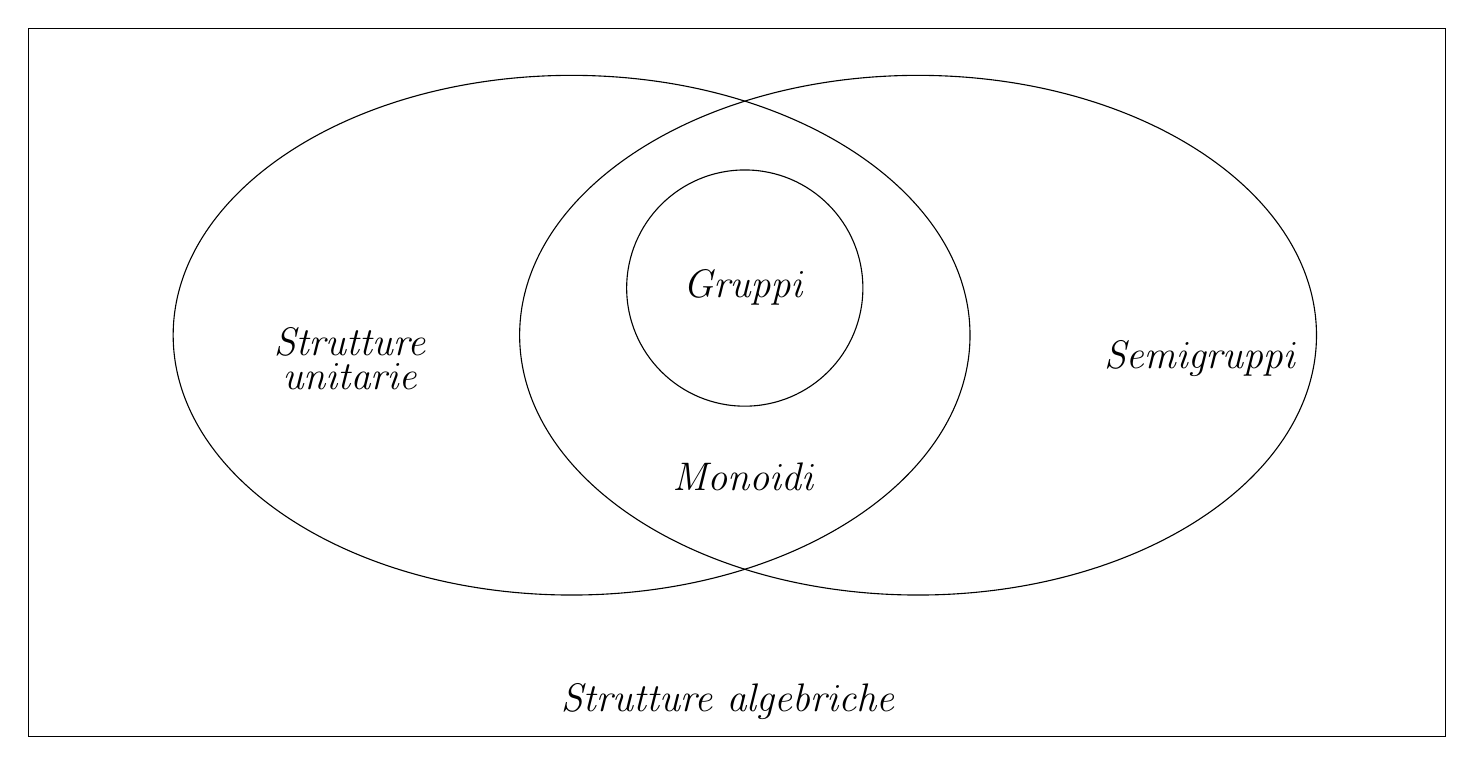
\begin{tikzpicture}
		% Define the size of the rectangle
		\draw[draw=black] (9.1, 6.2) rectangle ++(18, 9);
		
		% Calculate the center of the rectangle and move it on the y-axis
		\coordinate (center) at (16, 11.3);
		
		\begin{scope}
			% Create the first circle
			\draw[xscale=2.3, yscale=1.5] (center) circle (2.2cm);
		\end{scope}
		
		
		
		\begin{scope}
			% Calculate the position for the third circle relative to the center and move it on the y-axis
			\coordinate (thirdCircle) at ([xshift=2.2cm, yshift=0.6cm] center);
			
			% Create the third circle
			\draw (thirdCircle) circle (1.5cm);
			
			% Text inside the third circle
			\node[align=center, text width=5cm,] at (thirdCircle) {\Large{\textit{Gruppi}}};
		\end{scope}
		
		\begin{scope}
			% Calculate the position for the second circle relative to the center
			% Reduce the xshift to make the circles overlap more
			\coordinate (secondCircle) at ([xshift=4.4cm] center);
			
			% Create the second circle
			\draw[xscale=2.3, yscale=1.5] (secondCircle) circle (2.2cm);
		\end{scope}
		% Text
		\begin{scope}
			\node[align=center, xshift=13.2cm, yshift=11cm] {\Large{\textit{Strutture}}\\ \Large{\textit{unitarie}}};
			\node[below] at (18, 7) {\Large{\textit{Strutture algebriche}}};
			\node[align=center, xshift=24cm, yshift=11cm] {\Large{\textit{Semigruppi}}};
			\node[align=center, xshift=18.2cm, yshift=9.5cm] {\Large{\textit{Monoidi}}};
		\end{scope}
	\end{tikzpicture}
	\captionof{figure}{Strutture algebriche ad una singola operazione interna}
\end{center}

\marker{yellow!50}{yellow!20!black}{Per \textbf{gruppoide} si intende una struttura $(A,\bot)$ dotata di una operazione interna.\index{Gruppoide}}

\begin{center}
	\begin{tikzpicture}[every text node part/.style={align=center},rec/.style={fill=blue!20!white,rectangle,minimum height=1.5cm,minimum width=5cm},>=latex]
		\node[rec] (g) {\textbf{Gruppoide} $(A,\bot)$};
		\node[rec, below=1cm of g] (s) {\textbf{Semigruppo} \\ $\bot$ associativa};
		
		\node[rec,right=5cm of s](sa){\textbf{Semigruppo abeliano} \\ $\bot$ associativa \\ $\bot$ commutativa};
		\node[rec,below=1cm of sa] (ma){\textbf{Monoide abeliano} \\ $\bot$ associativa \\ $\exists u \in A (\forall a \in A (a \bot u=u \bot a = a))$ \\ $\bot$ commutativa};
		\node[rec,below=1cm of ma](ga){\textbf{Gruppo abeliano} \\ $\bot$ associativa \\ $\exists u \in A \bigl(\forall a \in A (a \bot u=u \bot a = a)\bigr)$ \\ $\forall x \in A \bigl(\exists x' (x \bot x'=u)\bigr)$ \\ $\bot$ commutativa};
		\node[rec, below=1cm of s](m){\textbf{Monoide} \\ $\bot$ associativa \\ $\exists u \in A (\forall a \in A (a \bot u =u \bot a =  a))$ };
		\node[rec,below=1.5cm of m](gr){\textbf{Gruppo} \\ $\bot$ associativa \\ $\exists u \in A \bigl(\forall a \in A (a \bot u=u \bot a = a)\bigr)$ \\ $\forall x \in A \bigl(\exists x' (x \bot x'=u)\bigr)$};
		\draw[->] (g) to node[midway,right]{$\bot$ associativa}(s);
		\draw[->] (s) to node[midway,right]{Esiste elemento neutro}(m);
		\draw[->] (m) to node[midway,right]{Esistono simmetrici}(gr);
		\draw[->](s) to node[midway,above]{$\bot$ commutativa}(sa);
		\draw[->](m) to node[midway,above]{$\bot$ commutativa}(ma);
		\draw[->](gr) to node[midway,above]{$\bot$ commutativa}(ga);
		\draw[->] (sa) to node[midway,right]{Esiste elemento neutro}(ma);
		\draw[->] (ma) to node[midway,right]{Esistono simmetrici}(ga);
	\end{tikzpicture}
	\captionof{figure}{Caratterizzazione delle strutture ad una singola operazione interna}
\end{center}

\section{Anelli}

\begin{defbox}{Anello}\index{Anello}
	Un \textbf{anello} è un insieme $A$ dotato di due operazioni $+$, $\cdot$ (che saranno sempre chiamate ``somma'' e ``prodotto''), che soddisfano le seguenti proprietà:
	\begin{enumerate}
		\item $(G,+)$ è un gruppo abeliano:
		\begin{enumerate}
			\item $+$ è associativa
			\item $+$ è commutativa
			\item Esiste l'elemento neutro rispetto a $+$ ed è denotato con $0_{G}$
			\item Per ogni $x \in G$ esiste $-x \in G$ tale che $x+(-x)=0_{G}$.
		\end{enumerate}
		\item $(G,\cdot)$ è un semigruppo
		\item L'operazione $\cdot$ è distributiva rispetto a $+$:
		\begin{displaymath}
			\forall a,b,c \in A \begin{cases}
				a \cdot (b+c) = ab + ac \\
				(a+b)c = ac + bc
			\end{cases}
		\end{displaymath}
	\end{enumerate}
	Se anche l'operazione $\cdot$ è commutativa allora l'anello si dice \textbf{abeliano}. Se esiste l'elemento neutro per la moltiplicazione\footnote{Quindi $(A,\cdot)$ è un monoide} indicato con $1_{A}$ allora l'anello si dice \textbf{unitario}.
\end{defbox}
\begin{example}
	Sono anelli, con le usuali operazioni di somma e prodotto, gli insiemi numerici $\mathbb{R}, \mathbb{Z}, \mathbb{Q}, \mathbb{C}$.
\end{example}
\begin{example}
	Dato l'insieme $E=\{a,b,c\}$ consideriamo l'insieme delle parti $\mathcal{P}(E)$: $$\mathcal{P}(E)= \{\emptyset, \{a\}, \{b\}, \{c\}, \{a,b\}.\{b,c\},\{a,c\},E\}$$ Consideriamo in tale insieme le due operazioni di differenza simmetrica $\triangle$ e di intersezione $\cap$. È facile verificare che la struttura $(\mathcal{P}(E),\triangle,\cap)$ è un anello:
	\begin{enumerate}
		\item L'operazione $\triangle$ è associativa e commutativa;
		\item Esiste l'elemento neutro rispetto a $\triangle$, ovvero l'elemento: $\emptyset$: $\forall x \in \mathcal{P}(E) \bigl(a \triangle \emptyset = \emptyset \triangle a = a\bigr)$;
		\item Ogni elemento $ a \in \mathcal{P}(E)$ ha come simmetrico se stesso rispetto a $\triangle$: $a \triangle a = (a \cup a ) \setminus (a \cap a) = \emptyset$. Quindi $(\mathcal{P}(E),\triangle)$ è un gruppo;
		\item L'operazione $\cap$ è associativa e commutativa;
		\item Esiste l'elemento neutro rispetto a $\cap$, ovvero $E$ e vale: $\forall a \in \mathcal{P}(E) \bigl(a \cap e = e \cap a = a \bigr)$;
		\item L'intersezione è distributiva rispetto alla differenza simmetrica: $$\forall a,b,c \in \mathcal{P}(E) \bigl(a \cap (b \triangle c) = (a \cap b) \triangle (a \cap c)\bigr)$$
	\end{enumerate}
	Pertanto la struttura $(\mathcal{P}(E),\triangle,\cap)$ è un anello commutativo unitario. Tale anello prende il nome di \textbf{anello di Boole}.
\end{example}



\subsection{Regole di calcolo in un anello}
Dagli assiomi che definiscono la struttura di anello, seguono di fatto molte di quelle proprietà delle operazioni che utilizziamo familiarmente nel caso di anelli numerici. Le elenchiamo nelle seguenti proposizioni: la prima riguarda la somma, e non è altro che la \textbf{legge di cancellazione}, valida in qualsiasi gruppo; la seconda riguarda il prodotto (si osservi come sia fondamentale la proprietà distributiva).

\begin{propbox}	
	Sia $A$ un anello. Allora, per ogni $a,b,c \in A$:
	\begin{equation}
		a+b = a+c  \implies b=c
	\end{equation}
\end{propbox}
\begin{proof}
	Siano per ogni $a,b,c \in A$, tali che $a+b=a+c$ e sia $a'\in A$ tale che $a'+a=0_{A}$. Allora:
	\begin{align*}
		b &= 0_{A}+b  & \text{\textcolor{gray}{(elemento neutro della somma)}}\\
		&= (a+a')+b & \text{\textcolor{gray}{(elemento opposto)}}\\
		&= a' + (a+b) & \text{\textcolor{gray}{(proprietà associativa)}}\\
		&=a' + (a+c) & \text{\textcolor{gray}{(per ipotesi)}} \\
		&=(a'+a)+c  =0_{A}+c =c \\
	\end{align*}
\end{proof}

Supponiamo ora che $0'_{A}$ sia un elemento neutro per la somma. Allora:
$	0'_{A} = 0'_{A}+0_{A}=0_{A}$. Infine, se $a'$ e $a''$ sono opposti dell'elemento $a$, allora $a+a'=0_{A}=a+a''$ e quindi, per quanto provato sopra, $a'=a''$. Se $a$ e $b$ sono elementi dell'anello $A$, si adotta la seguente notazione: $a-b=a+(-b)$. Nel caso del prodotto invece si è soliti scrivere direttamente: $a \cdot b = ab$.


\begin{propbox}
	Sia $A$ un anello unitario, e siano $a,b \in A$ allora:
	\begin{enumerate}
		\item Esiste un unico elemento neutro per il prodotto
		\item $a \cdot 0_{A}=0_{A} \cdot a=0_{A}$
		\item $a(-b)=-(ab)=(-a)b$
		\item $(-a)(-b)=ab$
	\end{enumerate}
\end{propbox}

\begin{proof}
	$(1)$ Siano $1_{A}$ e $1'_{A}$ elementi neutri per il prodotto. Allora, analogamente a quanto visto per l'addizione:
	\begin{displaymath}
		1'_{A} = 1'_{A} \cdot 1_{A} = 1_{A}
	\end{displaymath}
	
	$(2)$ Sia $c = a 0_{A}$. Allora, applicando la proprietà distributiva:
	\begin{align*}
		c &= a 0_{A} & \text{\textcolor{gray}{(per ipotesi)}}\\
		&= a(0_{A}+0_{A}) & \text{\textcolor{gray}{(idempotenza)}}\\
		&= a0_{A} +a0_{A} & \text{\textcolor{gray}{(proprietà distributiva)}}\\
		&= c+c\\
	\end{align*}
	e quindi $c=c+c-c=c-c = 0_{A}$. Analogamente si dimostra che $0_{a} a = 0_{A}$.
	
	$(3)$ Proviamo che $a(-b)=-(ab)$. Applicando la proprietà distributiva ed il punto 2:
	\begin{align*}
		a(-b)+ab&=a(-b+b)=a0_{A}=0_{A}
	\end{align*}
	e quindi $a(-b) =-(ab)$. Analogamente si dimostra che $(-a)b=-(ab)$.
	
	$(4)$ Per il punto 3 si ha:
	\begin{align*}
		(-a)(-b)&=-(a(-b))\\
		&=-(-(ab))\\
		&=ab
	\end{align*}
\end{proof}

Anche per un generico anello è possibile definire l'elevazione a potenza per un numero intero.  In generale, in un anello non commutativo, $A$ non è detto che, dati $a,b \in A$ e $n \in \mathbb{N}$ valga $(ab)^{n}=a^{n}b^{n}$. Tuttavia, non è difficile provare che se $ab=ba$ allora si ha, per ogni $n \in \mathbb{N}$, $(ab)^{n}=a^{n}b^{n}$. In particolare, questa ulteriore proprietà delle potenze sussiste negli anelli abeliani, nei quali vale il seguente teorema:

\begin{teorbox}
	[del binomio di Newton]\index{Binomio di Newton}
	Sia $A$ un anello commutativo, e siano $a,b \in A$. Per ogni $n \in \mathbb{N}$:
	\begin{equation}
		(a+b)^{n}= \sum_{i=0}^{n}\binom{n}{i}a^{n-i}b^{i}
	\end{equation}
\end{teorbox}

Questa formula non vale se l'anello non è commutativo. Per verificarlo basta osservare ciò che accade se si prova a calcolare $(a+b)^{3}$:
\begin{align*}
	(a+b)^{3} &= (a+b)(a+b)(a+b) \\
	&= a(a+b)(a+b) + b(a+b)(a+b) 	\\
	&= a(a(a+b) +b(a+b)) + b(a(a+b)+b(a+b))\\
	&= a(aa+ab +ba+bb) + b(aa+ab+ba+bb) \\
	&= aaa+aab+aba+abb + baa +bab + bba + bbb \\
\end{align*}

Se l'anello fosse commutativo si potrebbero unire i fattori $(aab+aba+baa)$ come $3a^{2}b$ e ottenere la formula indicata dal binomio di Newton ma essendo $ab \neq ba$ questo non è possibile e tutti i fattori sono uno diverso dall'altro.

\begin{defbox}{Sottoanello}\index{Sottoanello}
	Un sottoinsieme non vuoto $S$ di un anello $A$ che sia chiuso rispetto alle due operazioni di $A$ si dice \textbf{sottoanello} di $A$.
\end{defbox}

\subsection{Tipologie di anello}
La nozione di cancellabilità, come quella di invertibilità, riveste una grande importanza in teoria degli anelli. In questo contesto una prima precisazione, per quanto ovvia, è necessaria: \textit{ogni elemento di un anello è simmetrizzabile, quindi anche cancellabile, rispetto all'operazione additiva}, dunque quando si parla di elementi cancellabili o simmetrizzabili in un anello è all’operazione moltiplicativa che si fa riferimento. 

Nei paragrafi precedenti abbiamo provato alcune proprietà degli anelli, che per $\mathbb{Z}$ siamo abituati a considerare ``naturali''. Ora, $\mathbb{Z}$ soddisfa anche altre proprietà, quali il fatto che il prodotto di due elementi diversi da zero è diverso da zero. Questa legge non discende dagli assiomi di anello, esistono infatti anelli in cui questa legge non vale.

\begin{defbox}{Divisore dello zero}\index{Divisore!dello zero}
	Sia $(A,+,\cdot)$ un anello e sia $a \in A$. Allora:
	\begin{itemize}
		\item $a$ è un \textbf{divisore sinistro dello zero} in $A$ se e soltanto se esiste un elemento $b \in A$ tale che $b \neq 0_{A}$ e $ab=0_{A}$.
		\item $a$ è un \textbf{divisore destro dello zero} in $A$ se e soltanto se esiste un elemento $b \in A$ tale che $b \neq 0_{A}$ e $ba=0_{A}$.
		\item $a$ è un \textbf{divisore dello zero} in $A$ se e soltanto se esiste un elemento $b \in A$ tale che $b \neq 0_{A}$ e $ab=ba=0_{A}$.
	\end{itemize}
\end{defbox}

\begin{example}
	Un esempio di divisori dello zero si può trovare negli anelli di matrici; ad esempio, in $(M_{2}(\mathbb{R}),+,\cdot)$ ovvero l'anello delle matrici\index{Matrice} quadrate di dimensione $2$ con le operazioni di somma e prodotto righe per colonne si ha:
	\begin{displaymath}
		\begin{bmatrix}
			0 & 1 \\
			0 & 1
		\end{bmatrix}
		\begin{bmatrix}
			1 & 1 \\
			0 & 0
		\end{bmatrix}
		=
		\begin{bmatrix}
			0 & 0 \\
			0 & 0 \\
		\end{bmatrix}
	\end{displaymath}
\end{example}

\begin{teorbox}\label{thm:car_divisori_zero}
	Per ogni elemento $a \in A$ si ha che:
	\begin{itemize}
		\item $a$ è un divisore sinistro dello zero in $A$ se e soltanto se $a$ non è cancellabile a sinistra in $(A, \cdot)$;
		\item $a$ è un divisore destro dello zero in $A$ se e soltanto se $a$ non è cancellabile a destra in $(A, \cdot)$;
		\item $a$ è un divisore dello zero in $A$ se e soltanto se non è cancellabile in $(A,\cdot)$.
	\end{itemize}
	
\end{teorbox}

\begin{proof}
	Dimostriamo la prima delle equivalenze logiche, la seconda equivalenza si dimostra in maniera analoga mentre la terza discende dalla veridicità delle prime due equivalenze.
	
	$\implies)$ Sia $a$ un divisore sinistro dello zero in $A$. Allora, per definizione, esiste un elemento $b \in A$ tale che $ab=0_{A} \neq b$.  Chiaramente vale: $0_{A}= a \cdot 0_{A}$ eppure l'equivalenza $ab=a0_{A}$ non implica che $b = 0_{A}$. Quindi $a$ non è cancellabile a sinistra.
	
	$\impliedby)$ Se $a$ non è cancellabile a sinistra in $(A,\cdot)$ allora esistono $u$ e $v$ in $A$ tale che $au=av$ e $u \neq v$. Per tali $u$ e $v$:
	\begin{align*}
		au &= av\\
		au - av &= 0_{A}\\
		a(u-v) &= 0_{A}\\
	\end{align*}
	e quindi $a$ è un divisore sinistro dello zero.
\end{proof}


\begin{teorbox}
	In un anello con più di un elemento, lo zero ($0_{A}$) è un divisore dello zero.
\end{teorbox}

\begin{proof}
	Sia $|A|>1$ allora esiste un elemento $b \in A \setminus \{0_{A}\}$ per il quale $0_{A}= 0_{A}= b 0_{A}$ e quindi $0_{A}$ risulta un divisore dello zero. Ovviamente se $|A|=1$ le operazioni di somma e prodotto coincidono in quanto si ha $0_{A}=1_{A}$.
\end{proof}

\begin{defbox}{Anello integro}\index{Anello!integro}
	Un anello si dice \textbf{integro} se in esso vale la legge di annullamento del prodotto.
	
\end{defbox}

Con la terminologia appena introdotta, possiamo riformulare questa condizione in questo modo: un anello è integro se e solo se non ha divisori propri dello zero. Per quanto appena dimostrato, ciò equivale anche a dire che nell'anello in questione ogni elemento diverso da zero è cancellabile.

\begin{propbox}[Legge di annullamento del prodotto]\label{annullamento_prodotto}
	Sia $A$ un anello integro e siano $a,b \in A$ due elementi qualsiasi. Si ha allora:
	\begin{equation}
		ab = 0 \implies (a=0 \lor b=0)
	\end{equation}
\end{propbox}

\begin{defbox}{Dominio di integrità}\index{Dominio!di integrità}
	Un anello si dice un \textbf{dominio di integrità} se è un anello integro commutativo unitario.
\end{defbox}

\begin{propbox}[Legge di cancellazione]\index{Legge!di cancellazione}
	Sia $A$ un dominio di integrità, allora per ogni $a,b \in A$ e per ogni $c \neq 0_{A}$ si ha:
	\begin{equation}
		ac=bc  \implies a=b
	\end{equation}
	Possiamo formularne la definizione in uno qualsiasi dei seguenti modi, tra loro equivalenti: un dominio
	di integrità è:
	\begin{itemize}
		\item un anello commutativo integro;
		\item un anello commutativo in cui vale la legge di annullamento del prodotto;
		\item un anello commutativo in cui ogni elemento diverso da zero è cancellabile.
	\end{itemize}
\end{propbox}
\begin{teorbox}
	Un anello $(A,+,\cdot)$ è un dominio di integrità se è privo di divisori dello zero.
\end{teorbox}
\begin{proof}
	\begin{itemize}
		\item[$\implies$] Se l'anello è un dominio di integrità, per la Proposizione \ref{annullamento_prodotto}  vale la legge di annullamento del prodotto. Per assurdo, sia $x \in A$ un divisore dello zero, allora:
		\begin{align*}
			\exists y \in A \setminus \{0_{A}\}\bigl(xy=0\bigr)
		\end{align*}
	e dunque, per la legge di annullamento del prodotto, deve essere $x=0_{A} \lor y=0_{A}$ che va contro le ipotesi che siano entrambi non nulli. Quindi $A$ è privo di divisori dello zero.
	\item[$\impliedby$] Se nessun elemento è divisore dello zero, allora tutti gli elementi sono cancellabili per il Teorema \ref{thm:car_divisori_zero}. Dunque, se consideriamo:
	\begin{align*}
		\forall x,y \in A \bigl( x \neq 0_{A} \land xy = 0_{A} \implies y = 0_{A} \bigr)
	\end{align*}
Quindi $A$ è un dominio di integrità, come volevasi dimostrare.
	\end{itemize}
\end{proof}
\begin{defbox}{Corpo}\index{Corpo}
	Un anello unitario $A$ si dice \textbf{corpo} se ogni elemento non nullo di $A$ è invertibile.
\end{defbox}

\begin{defbox}{Campo}\index{Campo}
	Un \textbf{campo} è un corpo commutativo, ovvero un anello abeliano in cui ogni suo elemento non nullo è invertibile.
\end{defbox}


\begin{propbox}
	Ogni campo è un dominio di integrità.
\end{propbox}

\begin{proof}
	Un campo è un corpo commutativo, ed un corpo è un anello unitario. Un anello commutativo unitario è dominio di integrità se e soltanto
	se è privo di divisori dello zero. Ogni elemento di un campo, eccetto lo	zero, è invertibile, e dunque cancellabile. Un elemento cancellabile non può essere divisore dello zero, e quindi non esistono divisori dello zero. Dunque il campo è dominio di integrità.
\end{proof}

Non vale il viceversa, non tutti i domini di integrità sono dei campi. Ad esempio $(\mathbb{Z},+,\cdot)$ è un dominio di integrità ma non è un campo in quanto, ad esempio, il numero 2 non ha un inverso moltiplicativo in $\mathbb{Z}$. \textit{Ogni dominio di integrità finito}, però, \textit{risulta essere un campo}. La ragione sta nel fatto che in un dominio di integrità finito, ogni elemento non nullo deve necessariamente avere inverso moltiplicativo. Questo può essere dimostrato con un argomento di tipo combinatorio. Sia $D$ un dominio di integrità con $n$ elementi. Consideriamo l'elemento $a \in D$ con $a \neq 0_{D}$. La funzione $f: D \rightarrow D$ definita da $f(x) = ax$ è iniettiva. Infatti:
	\begin{align*}
		\forall x,y \in D (f(x) = f(x) \iff ax = ay)
	\end{align*}
e poiché $D$ è un dominio di integrità, vale la legge di cancellazione, cioè: $x=y$. Essendo $f$ una funzione iniettiva tra due insiemi equipotenti questa risulta essere anche suriettiva. Dunque deve esistere un elemento $b \in D$ tale che $ab= 1_{D}$ e $b$ risulta essere $a^{-1}$. Questo dimostra che ogni elemento non nullo ha un inverso moltiplicativo e $D$ è un campo.

\begin{center}
	\begin{tikzpicture}
		[every text node part/.style={align=center},rec/.style={fill=blue!20!white,rectangle,minimum height=1.5cm,minimum width=3cm},>=latex]
		\node[rec,name=a]{\textbf{Anello} \\ $(A,+,\cdot)$};
		\node[rec,name=a1, below of=a, yshift=-1cm]{$S \neq \emptyset$};
		\node[rec,name=a2,right of=a1,xshift=3cm]{$(S,+)$ è un gruppo};
		\node[rec,name=a3,right of=a2,xshift=6cm]{$\cdot$ è associativa \\ $\cdot$ è distributiva rispetto a $+$};
		\node[rec,name=ac,below of=a3, yshift=-2cm]{\textbf{Anello commutativo}};
		\node[rec,name=au,below of=a2, yshift=-2cm]{\textbf{Anello unitario}};
		\node[rec,name=c,below of=au,yshift=-2cm]{\textbf{Corpo}};
		\node[rec,name=d,below of=ac,yshift=-2cm]{\textbf{Dominio di integrità}};
		\node[rec,name=k,below of=c,yshift=-2cm]{\textbf{Campo}};
		\draw[->,>=stealth](a)--(a1);
		\draw[->,>=stealth](a) -| (a2);
		\draw[->,>=stealth](a) -| (a3);
		\draw[->,>=stealth](a3) to node[right,midway]{$\cdot$ è commutativa} (ac);
		\path [draw, >=latex] (a3) |- ($(a3)+(0,-1.5)$) -| node[above,midway]{Se esiste $1_{A}$}(au);
		\draw[->,>=stealth](ac) to node[right,midway]{Se non ci sono \\ divisori dello zero}(d);
		\path [draw, >=latex] (au) -- ($(au)+(2,0)$) |-  node[midway,right]{Se non ci sono \\ divisori dello zero}(d);
		\draw[->](au) to node[left,midway]{Se ogni elemento\\ non nullo è invertibile rispetto a $\cdot$}(c);
		\draw[->](c) to node[left,midway]{Se $\cdot$ è commutativa}(k);
		\draw[->,>=stealth](d) |- node[right,midway]{Se ogni elemento \\ non nullo è invertibile \\ rispetto a $\cdot$}(k);
	\end{tikzpicture}
	\captionof{figure}{Caratterizzazione dei corpi}
\end{center}
\newpage
\section{Esercizi svolti}
\begin{exsbox}
	Sia $A=\{1,2\}$ e consideriamo l'operazione di intersezione nell'insieme delle parti di A:
	\begin{displaymath}
		\cap : \mathcal{P}(A) \times \mathcal{P}(A) \longrightarrow \mathcal{P}(A)
	\end{displaymath}
	Si rappresenti la relativa tavola di Cayley.
\end{exsbox}
\paragraph*{Svolgimento.} Si ha:
\begin{center}
	\begin{tblr}{
			hlines,
			vlines,
			row{1}={primary!80!white},
			column{1}={primary!80!white},
			cells={mode=math}
		}
		\cap & \varnothing & \{1\} & \{2\} & A \\
		\varnothing & \varnothing & \varnothing & \varnothing & \varnothing \\
		\{1\} & \varnothing & \{1\} & \varnothing & \{1\} \\
		\{2\} & \varnothing & \varnothing & \{ 2\} & \{2\} \\
		A & \varnothing & \{1\} & \{2\} & A \\
	\end{tblr}
\end{center}
\begin{flushright}
	\blacksquare
\end{flushright}
\begin{exsbox}
	Vero o falso? Per ogni insieme non vuoto $S$ ed ogni operazione binaria $\ast$ in S,...
	\begin{enumerate}
		\item In $S$ esiste sempre un elemento neutro a destra o un elemento neutro a sinistra;
		\item Se $\ast$ è commutativa, tutti gli elementi neutri a destra in $(S,\ast)$ sono anche neutri a sinistra;
		\item Se $\ast$ è commutativa, in $S$ esiste al massimo un elemento neutro a sinistra;
		\item Se $a$ e $b$ sono due elementi neutri a sinistra distinti in $(S, \ast)$, in $(S,\ast)$ non esistono elementi neutri a destra.
	\end{enumerate}
\end{exsbox}
\paragraph*{Svolgimento.} Sia $(S,\ast)$ un'arbitraria struttura algebrica.
\begin{enumerate}
	\item Falso. Ad esempio nell'insieme degli interi maggiori di 1 con l'operazione della moltiplicazione non esiste elemento neutro.
	\item Vero. Infatti se esiste un elemento $t \in S$ neutro a destra allora $\forall x \in S (x \ast t = t \ast x = x )$ e quindi $t$ è neutro a sinistra.
	\item Vero. Infatti, posto $u$ l'elemento neutro a sinistra, se esistesse un secondo elemento neutro a sinistra $u'$ si avrebbe:
	\begin{displaymath}
		u' = u \ast u' = u' \ast u = u
	\end{displaymath}
	\item Vero. Infatti se per assurdo esistesse un elemento neutro a destra, detto $u'''$, si avrebbe:
	\begin{displaymath}
		u'  \ast u''' = u'
	\end{displaymath}
	ma anche:
	\begin{displaymath}
		u'' \ast u''' = u''
	\end{displaymath}
	Tuttavia, poiché $u'$ e $u''$ sono elementi distinti si deve avere:
	\begin{displaymath}
		u' \ast u''' = u''' = u'' \ast u'''
	\end{displaymath}
	ma $u'' \neq u'$. \hfill \blacksquare
\end{enumerate}
\begin{exsbox}
	Dato l'insieme $A=\{0,1\}$ scrivere le tavole di Cayley di $(\mathcal{P}(A), \cup)$ e di $(\mathcal{P}(A), \triangle)$.
\end{exsbox}
\paragraph*{Svolgimento.} Si ha:
\begin{center}
	\begin{minipage}{.45\textwidth}
		\centering
		\begin{tblr}{
				hlines,
				vlines,
				row{1}={primary!80!white},
				column{1}={primary!80!white},
				cells={mode=math}
			}
			\cup & \varnothing & \{0\} & \{1\} & A \\
			\varnothing & \varnothing & \{0\} & \{1\} & A \\
			\{0\} & \{0\} & \{0\} & A & A \\
			\{1\} & \{1\} & A & \{1\} & A \\
			A & A & A & A & A
		\end{tblr}
	\end{minipage}
	\hfil
	\begin{minipage}{.45\textwidth}
		\centering
		\begin{tblr}
			{
				hlines,
				vlines,
				row{1}={primary!80!white},
				column{1}={primary!80!white},
				cells={mode=math}
			}
			\triangle & \varnothing & \{0\} & \{1\} & A \\
			\varnothing & \varnothing & \{0\}& \{1\} & A \\
			\{0\} & \{0\} & \varnothing & A & \{1\} \\
			\{1\} & \{1\} & A & \varnothing & \{0\} \\
			A & A & \{1\} & \{0\} & \varnothing
		\end{tblr}
	\end{minipage}
\end{center}
\begin{flushright}
	\blacksquare
\end{flushright}
\begin{exsbox}
	Studiare le operazioni binarie qui elencate, stabilendo per ciascuna di essere se è commutativa e se è associativa, e determinando gli elementi neutri a sinistra, a destra, neutri delle strutture da esse definite:
	\begin{enumerate}
		\item $\alpha: (a,b) \in \mathbb{N} \times \mathbb{N} \mapsto a 10^{b} \in \mathbb{N}$
		\item $\beta:(a,b) \in \mathbb{Z} \times \mathbb{Z} \mapsto -ab \in \mathbb{Z}$
		\item $\gamma:(a,b) \in \mathbb{Q} \times \mathbb{Q} \mapsto \frac{(a+b)}{2} \in \mathbb{Q}$
		\item $\delta: (a,b) \in \mathbb{Z} \times \mathbb{Z} \mapsto 2ab \in \mathbb{Z}$
		\item $\epsilon:(a,b) \in \mathbb{Q} \times \mathbb{Q} \mapsto 2ab \in \mathbb{Q}$
		\item $ \zeta : (a,b) \in \mathbb{Z} \times \mathbb{Z} \mapsto a+b+2 \in \mathbb{Z}$
		\item $\eta : (a,b) \in \mathbb{N} \times \mathbb{N} \mapsto a(b^{a+b}+3ab^{2})+1 \in \mathbb{N}$
		\item $\theta: (a,b) \in \mathcal{P}(\mathbb{Z})\times \mathcal{P}(\mathbb{Z}) \mapsto (a \cap \mathbb{N})\cup b \in \mathbb{Z}$
		\item $\iota : (a,b) \in \mathcal{P}(\mathbb{Z})\times \mathcal{P}(\mathbb{Z}) \mapsto a \cup b \cup \{1\} \in \mathbb{Z}$
	\end{enumerate}
\end{exsbox}
\paragraph*{Svolgimento.}
Si ha:
\begin{enumerate}
	\item L'operazione non è commutativa. Infatti:
	\begin{displaymath}
		\exists a,b \in \mathbb{N} (a 10^{b} \neq b 10^{a})
	\end{displaymath}
	ad esempio $(0,1)$.
	L'operazione non è associativa. Per essere associativa deve valere:
	\begin{displaymath}
		\forall a,b,c \in \mathbb{N}\quad  \bigl(	a \ \alpha \ (b \ \alpha \ c) = (a \ \alpha \  b) \ \alpha \ c  \bigr)
	\end{displaymath}
	ovvero:
	\begin{displaymath}
		a \cdot 10 ^{b \cdot 10 ^{c}} = a \cdot 10 ^{b+c}
	\end{displaymath}
	Scritto così è facile trovare una terna controesempio. Infatti sia $(1,1,2)$ si ha:
	\begin{displaymath}
		\begin{array}{l}
			a \cdot 10 ^{b \cdot 10 ^{c}} = 1 \cdot 10^{1 \cdot 10^{2}} = 10 ^{100}\\
			a \cdot 10 ^{b+c} = 1 \cdot 10^{1+2}= 1000
		\end{array}
	\end{displaymath}
	Si ha inoltre che $0 \in \mathbb{N}$ è neutro a destra rispetto ad $\alpha$, infatti:
	\begin{displaymath}
		\forall a \in \mathbb{N} (a \ \alpha \ 0 = a 10^{0} = a)
	\end{displaymath}
	A questo punto, per il \hyperlink{thm:neutro}{Teorema di unicità dell'elemento neutro}, se esiste un elemento neutro a sinistra deve essere proprio $0$ ma è evidente che $0$ non è neutro a sinistra.
	\item L'operazione è commutativa e associativa. Infatti:
	\begin{displaymath}
		\forall a,b \in \mathbb{Z} \bigl( a \ \beta \ b = -ab = -ba = b \ \beta \ a  \bigr)
	\end{displaymath}
	e
	\begin{displaymath}
		\forall a,b,c \in \mathbb{Z} \bigl(a \ \beta \ (b \ \beta \ c) = a \ \beta \ (-bc) = -(a(-bc))= abc\bigr)
	\end{displaymath}
	ma anche:
	\begin{displaymath}
		\forall a,b,c \in \mathbb{Z} \bigl((a \ \beta \ b) \beta \ c = (-ab) \ \beta \ c = -(-ab)c=abc\bigr)
	\end{displaymath}
	L'elemento $-1$ risulta neutro rispetto a $\beta$, infatti:
	\begin{displaymath}
		\forall b \in \mathbb{Z} \bigl(-1 \ \beta \ b = -(-1b)=b = -(b(-1))=b \ \beta \ -1 \bigr)
	\end{displaymath}
	\item L'operazione risulta commutativa:
	\begin{displaymath}
		\forall a,b \in \mathbb{Q} \bigl( a \ \gamma \ b = \frac{a+b}{2} = \frac{b+a}{2} = b \ \gamma \ a \bigr)
	\end{displaymath}
	ma non associativa. Infatti:
	\begin{displaymath}
		\forall a,b,c \in \mathbb{Q} \bigl(a \ \gamma \ (b \ \gamma \ c ) = a \ \gamma (\frac{b+c}{2}) = \frac{a+ \frac{b+c}{2}}{2} = \frac{2a+b+c}{4}  \bigr)
	\end{displaymath}
	e \begin{displaymath}
		\forall a,b,c \in \mathbb{Q} \bigl((a \ \gamma \ b) \ \gamma \ c = \frac{\frac{a+c}{2}+c}{2}= \frac{a+b+2c}{4}\bigr)
	\end{displaymath}
	presa la terna $(1,1,0)$ si ha:
	\begin{align*}
		\frac{2a+b+c}{4}&=\frac{2+1+0}{4}\\
		&=\frac{3}{4}
	\end{align*}
	e
	\begin{align*}
		\frac{a+b+2c}{4}&=\frac{1+1+0}{4}\\
		&=\frac{2}{4}=\frac{1}{2}
	\end{align*}
	Per esistere elemento neutro a destra deve esistere un elemento $t \in \mathbb{Q}$ tale che:
	\begin{displaymath}
		\forall a \in \mathbb{Q} (t \ \gamma \ a = a)
	\end{displaymath}
	ovvero:
	\begin{align*}
		\frac{a+t}{2}&=a \\
		a+t &= 2a \\
		t &= 2a-a \\
		t&=a
	\end{align*}
	ma non esiste $t \in \mathbb{Q}$ uguale ad ogni numero razionale. Quindi non esiste elemento neutro a destra. Analogamente a sinistra.
	\item L'operazione $\delta$ è commutativa e associativa. Infatti:
	$$ \forall a,b \in \mathbb{Z} \bigl( a \ \gamma \ b = 2ab = 2ba = b \ \delta \ a\bigr) $$
	e:
	\begin{displaymath}
		\begin{array}{l}
			\forall a,b,c \in \mathbb{Z} \bigl( a \ \delta \ (b \ \delta \ c) = a \ \delta \ (2bc) = 4abc \bigr)\\
			\forall a,b,c \in \mathbb{Z} \bigl((a \ \delta \ b) \delta c = (2ab) \ \delta \ c = 4abc \bigr)
		\end{array}
	\end{displaymath}
	Non esiste elemento neutro rispetto a $\delta$, infatti se esistesse un elemento neutro a destra $t \in \mathbb{Z}$ si deve avere:
	\begin{eqnarray*}
		a \ \delta \ t &=& a \\
		2at &=& a \\
		t &=& \frac{a}{2a}=\frac{1}{2} \notin \mathbb{Z}
	\end{eqnarray*}
	\item A differenza di $\delta$, l'operazione $\epsilon$ è commutativa, associativa e gode di elemento neutro.
	\item L'operazione è commutativa. Infatti, per ogni $a,b \in \mathbb{Z}$ si ha:
	\begin{displaymath}
		a \ \zeta \ b = a+b+2 = b+a+2 = b  \ \zeta  \ a
	\end{displaymath}
	Per verificare l'associatività deve essere, qualsiasi siano gli elementi $a,b,c \in \mathbb{Z}$:
	\begin{displaymath}
		\begin{cases}
			a \zeta (b \ \zeta \ c) = a \ \zeta \ (b+c+2) = a+(b+c+2)+2=a+b+c+4 \\
			(a \ \zeta \ b) \ \zeta \ c = c \ \zeta \ (a \ \zeta \ b) =c + a + b +4
		\end{cases}
	\end{displaymath}
	quindi $\zeta$ è associativa.
	Per trovare l'elemento neutro partiamo dalla definizione :
	\begin{displaymath}
		\forall a \in \mathbb{Z} \bigl( a \ \zeta \ u = a  \iff a+u+2=a \bigr)
	\end{displaymath}
	L'elemento $-2 \in \mathbb{Z}$ è neutro quindi rispetto a $\zeta$.
	\item L'operazione non è associativa, non è commutativa e non ha elemento neutro. Davanti a formule poco maneggevoli è utile provare cercando terne che negano le proprietà cercate. Infatti data la coppia $(2,3)$ si ha:
	\begin{displaymath}
		2\ \eta \  3 = 2(3^{2+3}+3\cdot2\cdot3^{2})+1=595 \neq 205 = 3(2^{3+2}+3 \cdot 3 \cdot2^{2})+1 = 3 \  \eta \  2
	\end{displaymath}
	e data la terna $(0,0,1)$ si ha:
	\begin{displaymath}
		(0 \ \eta \ 0) \ \eta \ 1 = 5 \neq 1 = 0 \ \eta \ (0 \ \eta \ 1)
	\end{displaymath}
	Per quanto riguarda la verifica dell'esistenza dell'elemento neutro, dalla definizione di elemento neutro a sinistra si ha che $t \in \mathbb{N}$ è neutro a sinistra rispetto a $\eta$ se e solo se:
	\begin{displaymath}
		\forall b \in \mathbb{N} (t \ \eta \ b = b)
	\end{displaymath}
	Osservando la formula dell'operazione si nota che:
	\begin{displaymath}
		\forall a \in \mathbb{N} \bigl( a \ \eta \ 0 = 1 \bigr)
	\end{displaymath}
	da cui si deduce la non esistenza di un elemento neutro. Infatti non esiste un elemento $t \in \mathbb{N}$ tale che $t \ \eta \ 0 = 0$ in quanto abbiamo visto che questo darà sempre 1 come risultato.
	\item L'operazione non è commutativa, seguendo il metodo visto nell'esercizio precedente si può andare per tentativi. Preso $a=\{-1\}\subseteq \mathbb{Z}$ e $b=\{-2,3\}\subseteq \mathbb{Z}$ si ha:
	\begin{displaymath}
		a \ \theta \ b = (a \cap \mathbb{N}) \cup b = (\{-1\}\cap \mathbb{N})\cup b = \varnothing \cup \{-2,3\} = \{-2,3\}
	\end{displaymath}
	\begin{displaymath}
		b \ \theta \ a = (\{-2,3\} \cap \mathbb{N}) \cup \{-1\} = \{3\} \cup \{-1\} = \{-1,3\}
	\end{displaymath}
	mentre per l'associatività, deve valere:
	\begin{displaymath}
		\forall a,b,c \in \mathcal{P}(\mathbb{Z})\bigl( a \ \theta \ (b \ \theta \ c) = (a \ \theta \ b) \ \theta \ c \bigr)
	\end{displaymath}
	Dove:
	\begin{align*}
		a \ \theta \ (b \ \theta \ c) &= a \ \theta \bigl( (b \cap \mathbb{N}) \cup c \bigr) \\
		&= (a \cap \mathbb{N}) \cup \bigl( (b \cap \mathbb{N}) \cup c \bigr)
	\end{align*}
	e:
	\begin{align*}
		(a \ \theta \ b) \ \theta \ c &= \bigl((a \cap \mathbb{N}) \cup b\bigr) \ \theta \ c \\
		&= \Bigl( \bigl((a \cap \mathbb{N}) \cup b\bigr) \cap \mathbb{N} \Bigr) \ \cup \ c \\
		&= \Bigl((a \cap \mathbb{N} \cap \mathbb{N}) \cup (b \cap \mathbb{N} )\Bigr) \ \cup \ c & \text{\textcolor{gray}{Applicando la distributività}} \\
		&= \Bigl( a \cap \mathbb{N} \cup (b \cap \mathbb{N})  \Bigr) \cup c
	\end{align*}
	Quindi vale la proprietà associativa. Se un elemento $a \in \mathcal{P}(\mathbb{Z})$ è neutro a sinistra vale, per ogni $b \in \mathcal{P}(\mathbb{Z})$:
	\begin{displaymath}
		a \ \theta \ b = b
	\end{displaymath}
	ovvero:
	\begin{displaymath}
		(a \cap \mathbb{N}) \cup b = b
	\end{displaymath}
	Data questa condizione si ha sicuramente che:
	\begin{displaymath}
		(a \cap \mathbb{N} = \emptyset) \implies  (a \cap \mathbb{N}) \cup b = b
	\end{displaymath}
	Preso $a \subseteq \mathbb{Z} \wedge a \cap \mathbb{N} \neq \emptyset$ allora $$a \ \theta \ \emptyset = (t \cap \mathbb{N}) \cup \emptyset = t \cap \emptyset \neq \emptyset $$
	Quindi $a$ non è neutro a sinistra in quanto esiste una scelta di $b \in \mathcal{P}(\mathbb{Z})$ che non verifica la condizione: $\emptyset$. Un metodo alternativo per arrivare alla stessa conclusione è quello di osservare che per valere la condizione deve essere:
	\begin{displaymath}
		\forall b \in \mathcal{P}(\mathbb{Z})	\bigl( (a \cap \mathbb{N}) \subseteq b \bigr)
	\end{displaymath}
	quindi deve essere $a \cap \mathbb{N} = \emptyset$. In conclusione $\theta$ ha elementi neutri a sinistra e sono tutte le parti $a \in \mathbb{Z} \setminus \mathbb{N}$. Dati infiniti elementi neutri a sinistra, per il \hyperlink{thm:neutro}{Teorema di unicità dell'elemento neutro} possiamo dire che $(\mathcal{P}(\mathbb{Z}), \theta)$ non ha elementi neutri a destra.
	\item L'operazione è commutativa e associativa per la commutatività e l'associatività dell'unione. Un elemento $t$ è neutro se e solo se, per ogni $b \in \mathcal{P}(\mathbb{Z})$ si ha:
	\begin{displaymath}
		t \ \iota \ b = b \ \iota \ t  = b
	\end{displaymath}
	ovvero:
	\begin{displaymath}
		t \ \iota \ b = t \cup b \cup \{1\} = b
	\end{displaymath}
	ma per ogni scelta di $b$ non esiste un siffatto elemento neutro in quanto il loro composto tramite $\iota$ sarà sempre diverso da $b$. Per convincerci di questa affermazione consideriamo $b= \emptyset$:
	\begin{displaymath}
		t \ \iota \ \emptyset = t \cup \emptyset \cup \{1\} \neq \emptyset
	\end{displaymath}
\end{enumerate}
\begin{flushright}
	\blacksquare
\end{flushright}
\begin{exsbox}
	Ripetere l'esercizio precedente per l'operazione $\ast$ definita in $\{0,1,2,3\}$ da questa tavola di Cayley:
	\begin{center}
		\begin{tblr}{hlines,vlines, row{1}={primary!80!white},column{1}={primary!80!white},cells={mode=math}}
			\ast & 0 & 1 & 2 & 3 \\
			0    & 1 & 1 & 0 & 1 \\
			1    & 1 & 1 & 1 & 1 \\
			2    & 1 & 1 & 2 & 1 \\
			3    & 1 & 1 & 3 & 1 \\
		\end{tblr}
	\end{center}
\end{exsbox}
\paragraph*{Svolgimento.} Dall'osservazione diretta della tavola si può dire che l'operazione $\ast$ non è commutativa. Infatti, si ha:
\begin{displaymath}
	3 \ast 2 = 3 \neq 1 = 2 \ast 3
\end{displaymath}
L'elemento 2 è neutro a destra. Infatti $$\forall a \in \{0,1,2,3\} \bigl(a \ast 2 = a \bigr)$$
Per verificare l'associatività dell'operazione $\ast$ si procede confrontando se per ogni terna $(a,b,c)$ vale:
\begin{displaymath}
	a \ast (b \ast c) = (a \ast b) \ast c
\end{displaymath}
Se si trova una terna per la quale non vale la condizione di associatività si può concludere dicendo che l'operazione non è associativa. Il calcolo può essere ridotto osservando che, quando $c=2$ si ha:
\begin{displaymath}
	a \ast (b \ast 2) = a \ast b = (a \ast b) \ast 2
\end{displaymath}
Quindi il calcolo si riduce alle terne $(a,b,c)$ con $c \neq 2$. Anche in questo caso non esistono terne che contraddicono la condizione e allora l'operazione è associativa. \hfill \blacksquare
\begin{exsbox}
	Determinare gli elementi simmetrizzabili nel monoide $(\mathbb{R}, \cdot , 1)$ e, per un arbitrario insieme $A$, nei monoidi $(\mathcal{P}(A), \cup, \emptyset)$ e $(\mathcal{P}(A), \cap, A)$.
\end{exsbox}
\paragraph{Svolgimento.} 	All'interno del monoide $(\mathbb{R}, \cdot, 1)$ tutti gli elementi diversi da 0 sono simmetrizzabili. Infatti, per ogni $a\in \mathbb{R}\setminus \{0\}$ esiste un elemento $a^{-1}$ tale che $a \cdot a^{-1} = 1$. Tale simmetrico, detto inverso, è esattamente $1/a$. $(\mathbb{R}\setminus \{0\}, \cdot, 1)$ è quindi un gruppo.
\bigskip

Per un determinato insieme $A$, nei monoidi $(\mathcal{P}(A), \cap, A)$ e $(\mathcal{P}(A), \cup, \emptyset)$ gli unici elementi simmetrizzabili sono $A$ e $\emptyset$. Infatti, preso il primo monoide, l'unico elemento $a$ di $\mathcal{P}(A)$ per il quale esista un elemento $t \in \mathcal{P}(A)$ tale che:
\begin{displaymath}
	a \cup t = \emptyset
\end{displaymath}
è l'insieme vuoto stesso. Infatti: $\emptyset \cup \emptyset = \emptyset$. Analogamente, in $(\mathcal{P}(A), \cap, A)$ l'unico elemento $a \in \mathcal{P}(A)$ per il quale esiste un $t \in \mathcal{P}(A)$ tale che:
\begin{displaymath}
	a \cap t = A
\end{displaymath}
è $A$ stesso e risulta: $A \cap A = A$. \hfill \blacksquare
\begin{exsbox}
	Sia $\ast$ l'operazione binaria definita in $X \coloneqq \mathbb{Z} \times \mathbb{Z}$ da:
	\begin{displaymath}
		(\forall \ a,b,c,d \in \mathbb{Z})\bigl((a,b) \ast (c,d) =(ac,ad)\bigr)
	\end{displaymath}
	Decidere se $\ast$ è associativa, commutativa, se ammette elementi neutri a sinistra, se ne ammette a destra. Nel caso la richiesta abbia senso, determinare gli elementi simmetrizzabili in $(X, \ast)$, descrivendone i simmetrici. Che tipo di struttura (semigruppo, monoide, gruppo, commutativo o no?) è $(X, \ast)$?
\end{exsbox}
\paragraph*{Svolgimento.} L'operazione $\ast$ non è commutativa. Non vale cioè:
\begin{displaymath}
	\forall a,b,c,d \in \mathbb{Z} \bigl((a,b) \ast (c,d) = (c,d) \ast (a,b) \bigr)
\end{displaymath}
Infatti:
\begin{eqnarray*}
	(a,b) \ast (c,d) &=& (ac,ad) \\
	(c,d) \ast (a,b) &=& (ca,cb) \\
\end{eqnarray*}
L'operazione è però associativa:
\begin{displaymath}
	\forall a,b,c,d,e,f \in \mathbb{Z} \biggl( \Bigl((a,b)\ast(c,d)\Bigr)\ast (e,f)=  (a,b)\ast \Bigl((c,d)\ast (e,f)\Bigr)\biggr)
\end{displaymath}
Infatti:
\begin{eqnarray*}
	\Bigl((a,b)\ast(c,d)\Bigr)\ast (e,f) &=& (ac,ad) \ast (e,f) = (ace,acf) \\
	(a,b)\ast \Bigl((c,d)\ast (e,f)\Bigr) &=& (a,b) \ast (ce,cf) =(ace,acf)
\end{eqnarray*}
L'operazione non ha elementi neutri a destra. Infatti un tale elemento $(u,z)\in \mathbb{Z}\times \mathbb{Z}$ deve soddisfare alla proprietà, qualsiasi sia la coppia $(a,b)$:
\begin{displaymath}
	(a,b) \ast (u,z)= (au,az)=(a,b) \iff u=1 \wedge az=b
\end{displaymath}
ma $az=b$ se e solo se $z= 1 \wedge a=b$ oppure $a=1 \wedge z=b$ e quindi non esiste una siffatta coppia valida per tutti le coppie $(a,b)$. Esistono però infiniti elementi neutri a sinistra. Infatti:
\begin{displaymath}
	(u,z) \ast (a,b) = (ua,ub) = (a,b) \iff u=1
\end{displaymath}
Quindi ogni coppia del tipo $(1,x)\in \mathbb{Z}\times \mathbb{Z}$ è un elemento neutro a sinistra. La struttura quindi è un semigruppo. \hfill \blacksquare
\begin{exsbox}
	Stesse domande dell'esercizio precedente per le operazioni:
	\begin{enumerate}
		\item $\varphi:(a,b) \in \mathbb{Z} \times \mathbb{Z}  \mapsto a+b-1 \in \mathbb{Z}$
		\item $\psi : (a,b) \in \mathbb{Z} \times \mathbb{Z} \mapsto ab+1 \in \mathbb{Z}$
		\item $\mu : \bigl((a,b),(c,d)\bigr) \in (\mathbb{Z} \times \mathbb{Z}) \times (\mathbb{Z} \times \mathbb{Z}) \mapsto (a+bc,bd) \in (\mathbb{Z} \times \mathbb{Z})$
		\item $\tau:(X,Y)\in \mathcal{P}(\mathbb{Z}) \times \mathcal{P}(\mathbb{Z}) \mapsto (X \cup Y) \cap \mathbb{N} \in \mathcal{P}(\mathbb{Z})$
		\item $\omega: (X,Y)\in \mathcal{P}(\mathbb{Z}) \times \mathcal{P}(\mathbb{Z}) \mapsto (X \setminus Y) \cup \{1\} \in \mathcal{P}(\mathbb{Z})$
	\end{enumerate}
	al posto di $\ast$.\footnote{\textbf{Suggerimento:} per l'ultima operazione considerare terne $(X,Y,Z)$ di parti di $\mathbb{Z}$ tali che $X \subseteq Y \subseteq Z$.}
\end{exsbox}
\paragraph*{Svolgimento.} Si ha:
\begin{enumerate}
	\item L'operazione $\varphi$ è commutativa:
	\begin{displaymath}
		\forall a,b \in \mathbb{Z}(	a \ \varphi \  b = b \  \varphi \ a )
	\end{displaymath}
	Infatti:
	\begin{displaymath}
		a \ \varphi \  b = a+b-1=b+a-1= b \  \varphi \ a
	\end{displaymath}
	ed è anche associativa:
	\begin{displaymath}
		\forall a,b,c \in \mathbb{Z} \bigl( a \varphi (b \ \varphi \ c) = (a \ \varphi \ b) \ \varphi \ c \bigr)
	\end{displaymath}
	Infatti:
	\begin{eqnarray*}
		a \varphi (b \ \varphi \ c) &=& a \ \varphi \ (b+c-1) \\
		&=& a+(b+c-1)-1 \\
		&=& a+b+c-2
	\end{eqnarray*}
	analogamente, sfruttando la proprietà commutativa di $\varphi$:
	\begin{eqnarray*}
		(a \ \varphi \ b) \ \varphi \ c &=& c \ \varphi \ (a \ \varphi \ b) \\
		&=& c +a +b -2
	\end{eqnarray*}
	E per la proprietà commutativa dell'addizione si ha l'associatività di $\varphi$. Un elemento $u \in \mathbb{Z}$ è neutro rispetto a $\varphi$ se e solo se:
	\begin{displaymath}
		\forall a \in \mathbb{Z} \bigl( a \ \varphi \ u = u \ \varphi \ a = a \bigl)
	\end{displaymath}
	Quindi deve essere $u=1$. Gli elementi simmetrizzabili in $(\mathbb{Z}, \varphi)$ sono tutti e soli gli elementi tali che:
	\begin{displaymath}
		\exists a' \in \mathbb{Z} \bigl( a \ \varphi a' = a' \ \varphi \ a = 1 \bigr)
	\end{displaymath}
	Deve essere quindi: $a+a'-1=1$ ovvero $a'=2-a$. La struttura risulta quindi un gruppo abeliano.
	\item L'operazione $\psi$ è commutativa. Infatti:
	\begin{displaymath}
		\forall a,b \in \mathbb{Z} \bigl( a \ \psi \ b = b \ \psi \ a \bigr)
	\end{displaymath}
	Sviluppando i calcoli:
	\begin{eqnarray*}
		a \ \psi \ b &=& ab+1 \\
		b \ \psi \ a &=& ba+1
	\end{eqnarray*}
	L'operazione però non è associativa. Calcolando le due espressioni infatti:
	\begin{eqnarray*}
		a \ \psi \ (b \ \psi \ c) &=& a \ \psi \ (bc+1) \\
		&=& a(bc+1)+1 \\
		&=& abc +a+1
	\end{eqnarray*}
	e, sfruttando la commutatività dell'operazione:
	\begin{eqnarray*}
		(a \ \psi \ b) \ \psi c &=& c \ \psi \ (a \ \psi \ b) \\
		&=& cab+c+1
	\end{eqnarray*}
	le due formule infatti sono diverse. Presa una terna arbitraria come ad esempio $(1,2,3)$ si ha:
	\begin{displaymath}
		1 \cdot 2 \cdot 3 + 1 +1 = 8 \neq 10 = 3 \cdot 1 \cdot 2 + 3 +1
	\end{displaymath}
	Un elemento $u \in \mathbb{Z}$ è neutro se e solo se, per ogni $a \in \mathbb{Z}$ si ha:
	\begin{displaymath}
		\forall a \in \mathbb{Z} \bigl( a \ \psi \ u = u \ \psi \ a = a\bigr)
	\end{displaymath}
	dove $$a \ \psi \ u = au+1 = a \iff u = -1$$
	Un elemento $x \in \mathbb{Z}$ è simmetrizzabile invece se esiste $x'$ tale che:
	\begin{displaymath}
		x \ \psi \ x' = u
	\end{displaymath}
	Sviluppando i calcoli si ottiene:
	\begin{align*}
		x \ \psi \ x' = -1 &\iff xx'+1 =-1 \\
		&\iff xx'=-2 \\
		&\iff x'= \frac{-2}{x}
	\end{align*}
	Quindi gli unici elementi simmetrizzabili in $\mathbb{Z}$ rispetto a $\psi$ sono 2, -2, 1 e -1.
	\item L'operazione $\mu$ non è commutativa. Infatti, per essere commutativa, per ogni scelta di $a,b,c,d \in \mathbb{Z}$ deve valere:
	\begin{displaymath}
		(a,b) \ \mu \ (c,d) = (c,d) \ \mu \ (a,b)
	\end{displaymath}
	Ovvero:
	\begin{displaymath}
		(a+bc,bd)= (c+da,bd)
	\end{displaymath}
	Per osservare che l'operazione $\mu$ non gode della proprietà commutativa si consideri la seguente quaterna come controesempio: $(2,4,3,7)$. Infatti:
	\begin{eqnarray*}
		(2,4) \ \mu \ (3,7) = (2+12,28)= (14,28) \\
		(3,7) \ \mu \ (2,4) = (2+14,28) = (17,28)
	\end{eqnarray*}
	L'operazione è associativa. Infatti si ha, qualsiasi siano $a,b,c,d,e,f \in \mathbb{Z}$:
	\begin{displaymath}
		\bigl(	(a,b) \ \mu \ (c,d)\bigr) \ \mu \ (e,f) = (a+bc,bd) \ \mu \ (e,f) = (a+bc+dbe,dbf)
	\end{displaymath}
	e
	\begin{displaymath}
		(a,b) \ \mu \ \bigl(  (c,d) \ \mu \ (e,f) \bigr) = (a,b) \ \mu \ (c+de,df) = (a+bc+dbe,dbf)
	\end{displaymath}
	L'elemento $(0,1) \in \mathbb{Z}$ è neutro rispetto a $\mu$, infatti:
	\begin{displaymath}
		\forall (a,b)\in \mathbb{Z}\times \mathbb{Z} \quad (a,b) \ \mu \ (0,1)= (0,1) \ \mu \ (a,b) = (a,b)
	\end{displaymath}
	Chiaramente non esistono elementi neutri diversi da $(0,1)$, un siffatto elemento deve soddisfare alla condizione:
	\begin{displaymath}
		\forall (a,b)\in \mathbb{Z}\times \mathbb{Z} \quad \Bigl(\underbrace{\bigl((a,b) \ \mu \ (x,y)= (a,b)\bigr)}_{\mbox{neutro a destra}}\wedge \underbrace{\bigl( (x,y) \ \mu \ (a,b) = (a,b) \bigr)}_{\mbox{neutro a sinistra}} \Bigr)
	\end{displaymath}
	Prendendo la prima delle due condizioni e sviluppando si ottiene:
	\begin{displaymath}
		(a+bx,by)=(a,b)
	\end{displaymath}
	valida se e soltanto se:
	\begin{displaymath}
		\left\{
		\begin{array}{l}
			a+bx = a \\
			by=b
		\end{array}
		\right.
	\end{displaymath}
	che ammette come unica soluzione la coppia $(0,1)$. Escluso l'elemento neutro non esistono elementi simmetrizzabili rispetto a $\mu$.
	\item L'operazione $\tau$ è commutativa. Infatti, per ogni scelta delle parti $A,B \in \mathcal{P}(\mathbb{Z})$ si ha:
	\begin{displaymath}
		(A \ \tau \ B) = (A \cup B) \cap \mathbb{N} = (B \cup A) \cap \mathbb{N} = (B \ \tau \ A)
	\end{displaymath}
	L'operazione $\tau$ per essere associativa deve soddisfare alla condizione:
	\begin{displaymath}
		\forall A,B,C \in \mathcal{P}(\mathbb{Z}) \quad \bigl( A \ \tau (B \ \tau \ C) = (A \ \tau \ B) \ \tau \ C \bigr)
	\end{displaymath}
	Sviluppando i calcoli si ottiene:
	\begin{eqnarray*}
		A \ \tau \ (B \ \tau \  C ) &=& A \ \tau \ \bigl((B \cup C) \cap \mathbb{N}\bigr)\\
		&=& \Bigl( A \cup \bigl( (B \cup C) \cap \mathbb{N} \bigr)\Bigr) \cap \mathbb{N} \\
		&=& \Bigl( A \cup \bigl( (B \cap \mathbb{N}) \cup (C \cap \mathbb{N})\bigr)\Bigr) \cap \mathbb{N} \\
		&=& (A \cap \mathbb{N}) \cup \Bigl( (B \cap \mathbb{N}) \cap \mathbb{N} \cup (C \cap \mathbb{N}) \cap \mathbb{N} \Bigr) \\
		&=& (A \cap \mathbb{N}) \cup (B \cap \mathbb{N}) \cup (C \cap \mathbb{N})
	\end{eqnarray*}
	mentre:
	\begin{eqnarray*}
		(A \ \tau \ B ) \ \tau \ C &=& \bigl((A \cup B) \cap \mathbb{N} \bigr) \ \tau \ C \\
		&=& \Bigl(\bigl((A \cup B) \cap \mathbb{N}\bigr) \cup C \Bigr) \cap \mathbb{N} \\
		&=& \Bigl(\bigl( (A \cap \mathbb{N}) \cup (B \cap \mathbb{N})\bigr) \cup C \Bigr) \cap \mathbb{N} \\
		&=& (A \cap \mathbb{N}) \cup (B \cap \mathbb{N}) \cup (C \cap \mathbb{N})
	\end{eqnarray*}
	il che dimostra che l'operazione $\tau$ è associativa.
	Un elemento $U \in \mathcal{P}(\mathbb{Z})$ è neutro se per ogni elemento $A$ di $\mathcal{P}(\mathbb{Z})$ vale:
	\begin{displaymath}
		A \ \tau \ A = (A \cup U ) \cap \mathbb{N} = A
	\end{displaymath}
	ma osservando che $(A\cup U) \cap \mathbb{N} = A \iff A \cup U \subseteq \mathbb{N} \wedge (A \cup U) = A \wedge A \subseteq \mathbb{N}$. Quindi in via definitiva la condizione non vale per tutti gli insiemi $B \in \mathcal{P}(\mathbb{Z} \setminus \mathbb{N}) \subseteq \mathcal{P}(\mathbb{Z})$. Quindi non esiste elemento neutro e non avrà senso inoltre cercare elementi simmetrizzabili.
	\item L'operazione $\omega$ non è commutativa in quanto la differenza simmetrica non gode di tale proprietà:
	\begin{displaymath}
		\forall A, B \in \mathcal{P}(\mathbb{Z}) \ \bigl( (X \setminus Y) \cup \{1\} \neq (Y \setminus X) \cup \{1\}\bigr)
	\end{displaymath}
	Per verificare la proprietà associativa deve valere, per ogni $A,B,C \in \mathcal{P}(\mathbb{Z})$:
	\begin{displaymath}
		A \ \omega \ (B \ \omega \ C) = (A \ \omega \ B) \ \omega \ C
	\end{displaymath}
	Dove:
	\begin{eqnarray*}
		A \ \omega \ (B \ \omega \ C) &=& A \ \omega \ \bigl( (B \setminus C) \cup \{1\}\bigr) \\
		&=& (A \setminus (B \setminus C) \cap A \setminus \{1\}) \cup \{1\} \\
		&=& (A \setminus (B \setminus C))\cup \{1\} \cap A
	\end{eqnarray*}
	e:
	\begin{eqnarray*}
		(A \ \omega \ B) \ \omega \ C &=&\bigl( (A \setminus B) \cup \{1\}\bigr) \ \omega \ C \\
		&=& \Bigl( \bigl((A \setminus B) \cup \{1\} \bigr)\setminus C \Bigr) \cup \{1\}
	\end{eqnarray*}
	Che rappresentano insiemi diversi. Infatti, considerati gli insiemi:
	\begin{displaymath}
		\begin{array}{l}
			A = \{-3,4,5\} \\
			B = \{7,-5,3\} \\
			C = \{1,2,3\}
		\end{array}
	\end{displaymath}
	Si ha:
	\begin{displaymath}
		\begin{array}{l}
			A \ \omega \ (B \ \omega \ C) = (A \setminus (B \setminus C))\cup \{1\} \cap A  = A \\
			(A \ \omega \ B) \ \omega \ C = \Bigl( \bigl((A \setminus B) \cup \{1\} \bigr)\setminus C \Bigr) \cup \{1\} = A \cup \{1\}
		\end{array}
	\end{displaymath}
	Quindi $\omega$  non è associativa.
	Un elemento $U \in \mathcal{P}(\mathbb{Z})$ è neutro a destra se e solo se, per ogni parte di $\mathbb{Z}$ si ha:
	\begin{displaymath}
		A \ \omega \ U = A
	\end{displaymath}
	Ovvero:
	\begin{displaymath}
		(	A \setminus U) \cup \{1\} = A
	\end{displaymath}
	Ma:
	\begin{displaymath}
		\emptyset \ \omega \ U = \{1\} \neq \emptyset
	\end{displaymath}
	Quindi non esiste elemento neutro a destra in $\mathcal{P}(\mathbb{Z})$ rispetto a $\omega$. Analogamente a sinistra. \hfill \blacksquare
\end{enumerate}
\begin{exsbox}
	Sia $S=\{a,x,y\}$ un insieme di tre elementi e si consideri in $S$ l'operazione $\ast$ definita in $S$ da questa tavola di Cayley:
	\begin{center}
		\begin{tblr}{hlines,vlines, row{1}={primary!80!white},column{1}={primary!80!white},cells={mode=math}}
			\ast & a & x & y \\
			a & a & x & y \\
			x & x & a & a \\
			y & y & y & a \\
		\end{tblr}
	\end{center}
	Dopo aver verificato che $a$ è neutro in $(S, \ast)$ e aver determinato i simmetrici destri e sinistri degli elementi di $S$, senza fare ulteriori calcoli si decida se $(S, \ast, a)$ è un monoide.
\end{exsbox}
\paragraph*{Svolgimento.} Una struttura algebrica, per essere un monoide deve essere associativa la sua operazione interna ed esistere l'elemento neutro. Osservando la tavola di Cayley si ha che $a$ è elementro neutro. Osservando i simmetrici destri e sinistri degli elementi di $S$ notiamo però che:
\begin{displaymath}
	x \ \ast \ x = x \ \ast \ y = a
\end{displaymath}
e se $\ast$ fosse associativa questo non dovrebbe essere possibile. Infatti in un semigruppo ogni elemento ha al più un simmetrico destro e/o sinistro. Quindi possiamo concludere dicendo che $(S, \ast, a)$ non è un monoide.\hfill \blacksquare
\begin{exsbox}
	Verificare che se $\ast$ è un'operazione associativa, anche la sua operazione opposta è associativa.
\end{exsbox}
\paragraph*{Svolgimento.} Se l'operazione $\ast$ è associativa allora vale, per ogni elemento $a,b,c \in S$:
\begin{displaymath}
	a \ \ast \ (b \ \ast \ c) = (a \ \ast \ b) \ \ast \ c
\end{displaymath}
L'operazione opposta $\ast^{\ast}$ definita ponendo:
\begin{displaymath}
	a \ \ast^{\ast} \ b \coloneqq b \ \ast \ a
\end{displaymath}
sarà associativa se e solo se:
\begin{displaymath}
	a \ \ast^{\ast} \ (b \ \ast^{\ast} \ c) = (a \ \ast^{\ast} \ b) \ \ast^{\ast} \ c
\end{displaymath}
Si ha:
\begin{align*}
	a \ \ast^{\ast} \ (b \ \ast^{\ast} \ c) &= a \ \ast^{\ast} \ (c \ \ast \ b) & \text{\textcolor{gray}{Applicando la definizione di $\ast^{\ast}$}} \\
	&= (c \ \ast \ a) \ \ast \ a & \text{\textcolor{gray}{Applicando la definizione di $\ast^{\ast}$}} \\
	&= c \ \ast \ (b \ \ast \ a) & \text{\textcolor{gray}{Applicando l'associatività di $\ast$}} \\
	&= (a \ \ast^{\ast} \ b ) \ \ast^{\ast} \ c  & \text{\textcolor{gray}{Applicando la definizione di $\ast^{\ast}$}}
\end{align*}
E l'asserto è dimostrato. \hfill \blacksquare
\begin{exsbox}
	Nel monoide delle parole\footnote{Rispetto all'operazione di concatenazione} su un alfabeto che contenga la lettera $y$, dire se sono o non sono parti chiuse: l'insieme delle parole di lunghezza (nel senso ovvio) maggiore di $55$; l'insieme delle parole di lunghezza pari; l'insieme delle parole che iniziano per $y$; l'insieme delle parole che finiscono per $yyy$; l'insieme delle parole in cui $y$ appare al massimo tre volte; l'insieme delle parole che se hanno lunghezza maggiore di $10$ allora non hanno $y$ tra le lettere che vi appaiono.
\end{exsbox}
\paragraph*{Svolgimento.} Si ha:
\begin{itemize}
	\item L'insieme delle parole di lunghezza maggiore di 55 è una parte chiusa. Infatti concatendando due o più parole di questo insieme la stringa risultante sarà sempre di lunghezza maggiore di 55 caratteri;
	\item L'insieme delle parole di lunghezza pari è una parte stabile.
	\item L'insieme delle parole che iniziano per $y$ è una parte stabile;
	\item L'insieme delle parole che terminano per $yyy$ è una parte stabile;
	\item L'insieme delle parole in cui $y$ appare al massimo tre volte non è una parte stabile;
	\item L'insieme delle parole che se hanno lunghezza maggiore di 10 allora non hanno $y$ tra le lettere non è una parte stabile. \hfill \blacksquare
\end{itemize}
\begin{exsbox}
	In $D \coloneqq \mathbb{Z} \times \mathbb{Z}$ si definiscano le operazioni binarie $\ast$ e $\bot$ ponendo, per ogni $a,b,c,d \in \mathbb{Z}$ $$\bigl((a,b) \ast (c,d) = (ac,b+d)\bigr)$$ e per ogni $a,b,c,d \in \mathbb{Z}$ $$\bigl((a,b) \bot (c,d) = (ac,b-d)\bigr)$$ Studiare $(D,\ast)$ e $(D, \bot)$, decidendo che genere di strutture algebriche siano e, nel caso la domanda abbia senso, quali siano i loro elementi simmetrizzabili. Stabilire poi se $\mathbb{Z} \times \{0\}$ e $\mathbb{Z} \times \{1\}$ sono o non sono parti chiuse rispetto a $\ast$ o rispetto a $\bot$ e studiare, ove esistano, le corrispondenti strutture indotte.
\end{exsbox}
\paragraph*{Svolgimento.} \begin{enumerate}
	\item Iniziamo studiando l'operazione $\ast$. Per essere associativa, deve valere, $forall a,b,c,d,e,f \in \mathbb{Z}$,
	\begin{displaymath}
		(a,b) \ast \bigl((c,d) \ast (e,f)\bigr) = \bigl((a,b) \ast (c,d)\bigr) \ast (e,f)
	\end{displaymath}
	Applicando la definizione di $\ast$:
	\begin{align*}
		(a,b) \ast \bigl((c,d) \ast (e,f)\bigr) &= (a,b) \ast (ce, d+f)\\
		&= (ace,b+d+f)
	\end{align*}
	e:
	\begin{align*}
		\bigl((a,b) \ast (c,d)\bigr) \ast (e,f) &= (ac,b+d) \ast (e,f)\\
		&= (ace,b+d+f)
	\end{align*}
	Quindi $\ast$ è associativa e la struttura $(D,\ast)$ è un semigruppo. Per verificare la commutatività verifichiamo se vale l'uguaglianza, per ogni $a,b,c,d \in \mathbb{Z}$:
	\begin{displaymath}
		(a,b) \ast (c,d) = (c,d) \ast (a,b)
	\end{displaymath}
	la cui verifica è diretta osservando che le operazioni di addizione e moltiplicazione sono commutative:
	\begin{displaymath}
		(ac,b+d)=(ca,d+b)
	\end{displaymath}
	Quindi $(D,\ast)$ è un semigruppo commutativo. Verifichiamo adesso l'esistenza dell'elemento neutro. Essendo $\ast$ commutativa possiamo effettuare tale ricerca componendo sia a destra che a sinistra. Una coppia di numeri interi positivi è elemento neutro rispetto ad $\ast$ se, per ogni $a,b \in \mathbb{Z}$:
	\begin{displaymath}
		(a,b) \ast (u,l) = (a,b)
	\end{displaymath}
	Ovvero se:
	\begin{displaymath}
		(au,b+l) = (a,b)
	\end{displaymath}
	E ciò accade se e solo se $u=1$ e $l=0$. Quindi la coppia $(1,0)$ risulta essere elemento neutro rispetto a $\ast$ e $(D,\ast)$ risulta essere un monoide commutativo. Ci chiediamo ora quali coppie siano simmetrizzabili. Per definizione di elemento simmetrizzabile, una coppia $(a,b)$ ammette simmetrico se esistono $a',b'$ tali che $(a,b) \ast (a',b')=(1,0)$. Svolgendo i calcoli si ottiene:
	\begin{align*}
		(a,b) \ast (a',b') = (1,0) \iff (aa',b+b')=(1,0) \iff \begin{cases}
			a' = a^{-1} \\
			b' = -b
		\end{cases}
	\end{align*}
	Dato che gli unici elementi di $\mathbb{Z}$ ad ammettere inverso sono 1 e -1 mentre tutti gli elementi di $\mathbb{Z}$ ammettono opposto possiamo concludere dicendo che gli elementi simmetrizzabili in $(D,\ast)$ sono tutte e sole le coppie del tipo $(1,b)$ e $(-1,b)$ con $b \in \mathbb{Z}$. Quindi, in particolare $(D,\ast)$ non risulta essere un gruppo. Consideriamo ora gli insiemi $\mathbb{Z} \times \{0\} = \{(a,0) \; | \; a \in \mathbb{Z}\}$. Componendo due elementi di tale insieme si ottiene:
	\begin{displaymath}
		(a,0) \ast (b,0) = (ab,0)
	\end{displaymath}
	che è ancora un elemento di $\mathbb{Z} \times \{0\}$ e $(\mathbb{Z}\times \{0\},\ast_{\mathbb{Z}\times\{0\}})$ è una parte stabile di $(D,\ast)$.
	\item Consideriamo adesso l'operazione $\bot$ e verifichiamo se vale la proprietà associativa. Per ogni coppia $(a,b),(c,d),(e,f)$ abbiamo:
	\begin{displaymath}
		\bigl((a,b)\bot(c,d)\bigr)\bot(e,f)=(ac,b-d)\bot(e,f)=(ace,b-d-f)
	\end{displaymath}
	e
	\begin{displaymath}
		(a,b) \bot \bigl((c,d)\bot(e,f)\bigr)=(ace,b-d+f)
	\end{displaymath}
	Quindi $(D,\bot)$ non è un semigruppo e non ha senso continuare con lo studio. \hfill \blacksquare
\end{enumerate}
\begin{exsbox}
	Sia $S=\{0,1\}$. Elencare gli elementi di $T(S)$ e scrivere la tavola di Cayley di $T(S)$.
\end{exsbox}
\paragraph{Svolgimento.} Si ha $T(S)=\{id_{S},c_{0},c_{1},\sigma\}$ dove $\sigma$ è la trasposizione che sposta 0 in 1 e 1 in 0. Abbiamo quindi:
\begin{center}
	\begin{tblr}{hlines,vlines,row{1}={primary!80!white},cells={mode=math},column{1}={primary!80!white}}
		\circ & id_{S} & c_{0} & c_{1} & \sigma \\
		id_{S} & id_{S} & c_{0} & c_{1} &\sigma \\
		c_{0} & c_{0} & c_{0} & c_{0} & c_{0} \\
		c_{1} & c_{1} & c_{1} & c_{1} & c_{1}\\
		\sigma & \sigma & c_{1} & c_{0} & id_{S}
	\end{tblr}
\end{center}
\hfill \blacksquare
%  % Chapter 6: Reticoli
  \chapter{Reticoli e algebre di Boole}
\section{Relazioni d'ordine}

\begin{defbox}{Relazione d'ordine}\index{Relazione d'ordine}
	Sia $S$ un insieme non vuoto. Una relazione binaria $\rho$ in $S$ si dice una \textbf{relazione d'ordine largo} se è:
	\begin{enumerate}
		\item \textbf{Riflessiva}: $\forall x \in S \bigl(x \ \rho \ x \bigr)$;
		\item \textbf{Antisimmetrica}: $\forall x,y \in S \bigl((x \ \rho \ y \wedge y \ \rho \ x) \Rightarrow x = y\bigr)$;
		\item \textbf{Transitiva}: $\forall x,y,z \in S \bigl((x \ \rho \ y) \wedge (y \ \rho \ z) \Rightarrow x \ \rho \ z \bigr)$.
	\end{enumerate}
	Una relazione binaria $\rho$ in $S$ si dice una \textbf{relazione d'ordine stretto} se è :
	\begin{itemize}
		\item \textbf{Antiriflessiva:} $\forall x \in S \bigl(x \ \cancel{\rho} \ x\bigr)$.
		\item \textbf{Transitiva}
	\end{itemize}
\end{defbox}

\begin{osservation}
	Chiaramente ogni relazione di ordine stretto è necessariamente antisimmetrica. Infatti, sia $\rho$ una relazione di ordine stretto e siano $x,y \in A$ tali che $x \ \rho \ y \land y \ \rho \ x$. Per la proprietà transitiva deve essere $x \ \rho \ x $ ma per ipotesi $\rho$ è antiriflessiva. Questo vuol dire che non può essere $x \ \rho \ y \land y \ \rho \ x$ e quindi risulta vera l'implicazione $\bigl(x \ \rho \ y \land y \ \rho \ x \bigr)\implies (x=y)$ in quanto l'antecedente risulta falsa.
\end{osservation}
 Una relazione d'ordine in $S$ è in genere denotata, col simbolo $\leq$.
\begin{propbox}
	Sia $\mathbf{OL(A)}$ l'insieme di tutte le relazioni di ordine largo in $A$ e $\mathbf{OS(A)}$ l'insieme di tutte le relazioni di ordine stretto in $A$. Per ogni $\rho \in OL(A)$ è possibile definire $\rho_{\neq} \in Rel(A)$ in modo tale che, $\forall x,y \in A$:
	\begin{displaymath}
		\bigl(x \ \rho_{\neq} \ y \iff (x \ \rho \ y \land x \neq y ) \bigr) \implies \rho_{\neq} \in OS(A)
	\end{displaymath}
\end{propbox}

\begin{proof}
	Dimostriamo che la relazione $\rho_{\neq}$ gode della proprietà antiriflessiva e transitiva:
	\begin{itemize}
		\item \textbf{Antiriflessiva}: si ha che per ogni $x \in A (x \ \rho_{\neq} \ x)$ poiché $x=x$ e $x \ \rho \ x $ dato che $\rho \in OL(A)$;
		\item \textbf{Transitività}: per ogni $x,y,z \in A$ tali che $x \ \rho_{\neq} \ y \land y \ \rho_{\neq} \ z$ si ha:
		\begin{align*}
			\bigl(x \ \rho_{\neq} \ y \land y \ \rho_{\neq} \ z\bigr) &\implies (x \ \rho \ y \land x \neq y) \land (y \ \rho \ z \land y \neq z) & \text{\textcolor{gray}{Per ipotesi}}\\
			&\implies x \ \rho \ z \land x \neq z & \text{\textcolor{gray}{Sfruttando la transitività di $\rho$}}
		\end{align*}
	\end{itemize}
\end{proof}

\begin{propbox}
	Per ogni $\sigma \in OS(A)$ è possibile definire $\sigma_{=} \in Rel(A)$ in modo tale che, per ogni $x,y \in A$:
	\begin{displaymath}
		\bigl( x \ \sigma_{=} \ y \iff (x \ \sigma \ y \lor x = y ) \bigr) \implies \sigma_{=} \in OL(A)
	\end{displaymath}
\end{propbox}

\begin{proof}
	Dimostriamo che $\rho_{=}$ è riflessiva, antisimmetrica e transitiva:
	\begin{itemize}
		\item \textbf{Riflessiva:} per ogni $x \in A$ si ha $x \ \rho_{=} \ x $ poiché $x=x$;
		\item \textbf{Antisimmetria:} negando la proprietà devono esistere $x,y \in A$ per i quali $\bigl(x \ \sigma_{=} \ y \land y \ \sigma_{=} \ x \land x \neq y \bigr)$ il che sarebbe equivalente a dire che $\bigl( (x \ \sigma \ y \lor x = y) \land (y \ \sigma \ x \lor y=x) \land (x \neq y) \bigr)$, ovvero $(x \ sigma \ y) \land (y \ \sigma \ x) \land (x \neq y)$ il che è assurdo in quanto $\sigma$ è antisimmetrica. Quindi $\sigma_{=}$ è antisimmetrica.
		\item \textbf{Transitività:} per ogni $x,y,z \in A$ tali che $x \ \sigma \ y $ e $y \ \sigma \ z$ si ha:
		\begin{displaymath}
			x \ \sigma \ y \land y \ \sigma \ z \implies (x \ \sigma \ y \lor x = y) \land (y \ \sigma \ z \lor y=z) \\
		\end{displaymath}
		Nel caso in cui $x=y \land y = z$ si ha $x=z$, ovvero $x \ \sigma_{=} \ z$. Altrimenti, da $x \ \sigma \ y \land y \ \sigma \ z$ segue $x \ \sigma \ z$ e, per la transitività di $\sigma$ si ottiene $x \ \sigma_{=} \ z$.
	\end{itemize}
\end{proof}

\begin{propbox}
	Le applicazioni $\rho \in OL(A) \mapsto \rho_{=} \in OS(A)$ e $\sigma \in OS(A) \mapsto \sigma_{=} \in OL(A)$ sono biettive e l'una l'inversa dell'altra.
\end{propbox}

\begin{proof}
	Sia $\overline{\rho}$ la relazione duale di $\rho$ e sia $(\overline{\rho})^{\#}$ il suo grafico. Definiamo:
	\begin{enumerate}
		\item $\rho$ antiriflessiva se e soltanto se: $\Delta_{A} \cap \rho^{\#} = \emptyset$;
		\item $\rho$ antisimmetrica se e soltanto se: $\rho^{\#} \cap (\overline{\rho})^{\#} \subseteq \Delta_{A}$;
	\end{enumerate}
	Inoltre, si ha $(\rho_{\neq})^{\#} = \rho^{\#} \setminus \Delta_{A}$ e $(\sigma_{=})^{\#} = \sigma^{\#} \cup \Delta_{A}$. Allora il grafico di $(\rho_{\neq})_{=}$ risulta:
	\begin{align*}
		\bigl((\rho_{\neq})_{=}\bigr)^{\#} = \bigl(\rho^{\#} \setminus \Delta_{A}\bigr) \cup \Delta_{A}= \rho^{\#}
	\end{align*}
	dualmente per $(\sigma_{=})_{\neq}$
\end{proof}

\marker{yellow!40}{yellow!20!black}{
	La relazione identica $\iota_{S}$ è una relazione d'ordine in $S$, ed è chiaro che $\iota_{S}$ \textbf{è l'unica relazione di equivalenza in $S$ che sia anche una relazione d'ordine}.
}


\begin{osservation}
	Qualunque sia l'insieme $S$, la relazione binaria $\rho$ in $\mathcal{P}(S)$, definita ponendo:
	\begin{displaymath}
		x \ \rho \ y \Leftrightarrow x,y \in \mathcal{P}(S) \wedge x \subseteq y
	\end{displaymath}
	è una relazione d'ordine in $\mathcal{P}(S)$ chiamata \textbf{relazione di inclusione} e denotata con il simbolo $\subseteq$.
\end{osservation}


\begin{example}
	Un esempio di relazione d'ordine stretto è fornito dalla relazione binaria $\rho$, definita nell'insieme $\mathcal{P}(S)$ delle parti di un insieme $S$ ponendo:
	\begin{displaymath}
		x \ \rho \ y \Leftrightarrow x \subset y
	\end{displaymath}
	cioè se e soltanto se:
	\begin{displaymath}
		x \subseteq y \wedge x \neq y
	\end{displaymath}
	Tale relazione viene denotata col simbolo $\subset$.
\end{example}

\begin{example}\label{exmp:divisibilità}
	Sia $(\mathbb{N}, \cdot)$ un monoide abeliano. La relazione di divisibilità $\divides$ in $(\mathbb{N},\cdot)$ indicata da $\divides$ oppure da $\divides_{(\mathbb{N},\cdot)}$ è definita dalla formula:
	\begin{equation}
		\forall a,b \in S \bigl( a \divides b \iff \exists c \in \mathbb{N} (b = ac)\bigr)
	\end{equation}
	è una relazione di ordine parziale:
	\begin{enumerate}
		\item Per ogni $a \in \mathbb{N} \bigl( a \divides a \bigr)$, infatti $a = a \cdot 1$.
		\item Per ogni scelta di $a,b \in \mathbb{N}$, se $a \divides b$ e $b \divides a$, allora $a = b$: infatti esistono $q,q' \in \mathbb{N}$ tali che $b=a \cdot q$, $a=b \cdot q'$, quindi $a= a \cdot q \cdot q'$ e $a \cdot (1-q \cdot q') = 0$; se $a \neq 0$ deve essere $1-q \cdot q' = 0$, per cui $q = q' = 1$ e $a=b$; se invece $a=0$, anche $b=0$ e dunque nuovamente $a=b$;
		\item Per ogni scelta di $a,b,c \in \mathbb{N}$, se $a \divides b$ e $b \divides c$, allora $a \divides c$. Infatti, siano $q$ e $q' \in \mathbb{N}$ tali che $b= a \cdot q$ e $c = b \cdot q'$ allora $c = a \cdot (q \cdot q')$.
	\end{enumerate}
Altri risultati importanti sulla relazione di divisibilità saranno mostrati nella sezione \ref{sez:associati}.
\end{example}

\subsection{Insiemi ordinati}\label{sez:ordine}
\begin{defbox}{Insieme ordinato}
	Sia $S$ un insieme non vuoto e sia $\leq$ una relazione d'ordine in $S$. La coppia $(S, \leq)$ si chiama \textbf{insieme ordinato} (parzialmente), e l'insieme $S$ si dice \textbf{sostegno} di tale insieme ordinato.
	
\end{defbox}

\begin{example}
Sono insiemi ordinati:
		\begin{displaymath}
			\begin{array}{llll}
				(\mathbb{R},\leq) & (\mathbb{Q},\leq) & (\mathbb{Z}, \leq) & (\mathbb{N}, \leq)
			\end{array}
		\end{displaymath}
		dove $\leq$ è l'ordine usuale (ad esempio definito su $\mathbb{R}$ da $x \leq y$ se $y-x\geq0$, ovvero se esiste $a \in \mathbb{R}$ tale che $y-x=a^{2}$).
\end{example}

\begin{defbox}{Relazione d'ordine totale}
	Se $(S,\leq)$ è un insieme ordinato, gli elementi $x$ e $y$ di $S$ si dicono \textbf{confrontabili} se risulta $x \leq y$ oppure $y \leq x$, cioè se il grafico di $\leq$ contiene almeno una delle coppie $(x,y)$ e $(y,x)$. Se due qualunque elementi di $S$ sono confrontabili allora la relazione $\leq$ si dice una \textbf{relazione d'ordine totale} e la coppia $(S,\leq)$ è un \textbf{insieme totalmente ordinato}.
\end{defbox}

\begin{example}
\begin{enumerate}
		\item $(\mathcal{P}(X), \subseteq)$ non è un insieme totalmente ordinato se $X$ ha più di due elementi. Infatti, se $a_{1}, a_{2}$ sono elementi distinti di $X$, allora $\{a_{1}\}, \{a_{2}\} \in \mathcal{P}(X)$ e $\{a_{1}\} \nsubseteq \{a_{2}\}, \{a_{2}\}\nsubseteq \{a_{1}\}$. In questo caso diremo che $(\mathcal{P}(X),\subseteq)$ è un insieme \textbf{parzialmente ordinato}.
		\item L'insieme ordinato $(\mathbb{N}, \divides)$ non è totalmente ordinato. Basta considerare gli elementi 2 e 3 per vedere che $2 \ndivides 3$ e $3 \ndivides 2$.
		\item Gli insiemi $(\mathbb{R},\leq)$, $(\mathbb{Q},\leq)$, $(\mathbb{Z},\leq)$, dove $\leq$ è l'ordine usuale, sono totalmente ordinato.
\end{enumerate}
\end{example}

\begin{defbox}{Funzioni crescenti}
	Se $(S, \rho)$ e $(T,\sigma)$ sono insiemi ordinati, un'applicazione $f: S \rightarrow T$ si dice \textbf{crescente} se e soltanto se:
	\begin{equation}
		\forall a,b \in S \bigl(a \ \rho \ b \implies f(a) \ \sigma \ f(b) \bigr)
	\end{equation}
\end{defbox}

\begin{teorbox}[Isomorfismi tra insiemi ordinati]\label{thm:iso_ordinati}
	Siano $(S,\leq_{S})$ e $(T, \leq_{T})$ due insiemi ordinati. Si dice che $f: S \rightarrow T$ è un isomorfismo\footnote{Detto anche \textbf{isomorfismo d'ordine}} tra le strutture $(S,\leq_{S})$ e $(T,\leq_{T})$ se e soltanto se:
	\begin{enumerate}
		\item $f$ è biettiva;
		\item $f$ è crescente da $(S,\leq_{S})$ a $(T, \leq_{T})$: $\forall x,y \in S \bigl(x \leq_{S} y \implies f(x) \leq_{T} f(y) \bigr)$;
		\item $f^{-1}$ è crescente da $(T, \leq_{T})$ a $(S,\leq_{S})$: $\forall x,y \in T \bigl( x \leq_{T} y \implies f^{-1}(x) \leq_{S} f^{-1}(y) \bigr)$.
	\end{enumerate}
\end{teorbox}

\subsection{Minimo, massimo, minimali e massimali}
\begin{defbox}{Minimo e massimo di un insieme}
	Sia $(S,\leq)$ un insieme ordinato, e sia $X$ una parte non vuota di $S$. Un elemento $\bar{x}$ di $X$ si dice \textbf{minimo} di $X$ se risulta:
	\begin{displaymath}
		\forall x \in X \bigl( \bar{x} \leq x \bigr)
	\end{displaymath}
	L'eventuale minimo della parte non vuota $X$ di $S$ si denota col simbolo $min \ X$. Un elemento $\bar{\bar{x}} \in X$ si dice invece \textbf{massimo} se risulta:
	\begin{displaymath}
		\forall x \in X \bigl(x \leq \bar{\bar{x}}\bigr)
	\end{displaymath}
	L'eventuale massimo di $X$ si denota col simbolo $max \ X$.
	
\end{defbox}

\begin{defbox}{Elementi minimali e massimali}
	Sia $(S,\leq)$ un insieme ordinato. Un elemento $x$ di $S$ si dice \textbf{minimale} se non esiste alcun elemento $y$ di $S$ tale che $y < x$. Si dice invece che $x$ è un elemento \textbf{massimale} di $S$ se non esiste alcun elemento $y \in S$ tale che $x < y$.
\end{defbox}

Dalle definizioni segue, in particolare, che ogni elemento massimo (minimo) è anche un elemento massimale (minimale).  Non sempre, però, vale il contrario. Osserviamo anche che un insieme ordinato può avere diversi elementi minimali (o massimali). 

\begin{example}
	\begin{enumerate}
		\item Qualunque sia l'insieme $S$, nell'insieme ordinato $(\mathcal{P}(S), \subseteq)$ si ha:
		\begin{displaymath}
			\begin{array}{c}
				min \ \mathcal{P}(S) = \varnothing \\
				max \ \mathcal{P}(S) = S
			\end{array}
		\end{displaymath}
		
		\item L'insieme ordinato $(\mathbb{N}, \divides)$ ha minimo $1$, infatti $1 \divides n$ per ogni $n \in \mathbb{N}$, e massimo $0$, infatti $n \divides 0$ per ogni $n \in \mathbb{N}$. Se però togliamo $0$ e consideriamo $\mathbb{N}^{*}= \mathbb{N}\setminus\{0\}$, l'insieme ordinato $(\mathbb{N}^{*}, \divides)$ non ha massimo.
		\item Nell’insieme ordinato $ (\mathbb{N}\setminus \{1\}, \divides)$ dei numeri naturali diversi da 1 ordinato per divisibilità, gli elementi minimali sono tutti i numeri primi (positivi).
		\item Consideriamo, per un $n \in \mathbb{N}$, l'insieme $Div(n)=\{a \in \mathbb{N} \; | \; a \divides n\}$ dei divisori di $n$. Chiaramente in $(Div(n),\divides)$ si ha $min(Div(n))=1$ e $max(Div(n))=n$.
		
		\item Consideriamo l'insieme $\{1,2,3\}$ ordinato dalla divisibilità. Così:
	\begin{displaymath}
		1 \divides 2, \qquad 1 \divides 3, \qquad 2 \ndivides 3, \qquad 3 \ndivides 2
	\end{displaymath}
		Quindi 1 è minimo (minimale), mentre 2, 3 sono massimali, ma non massimi.
		\item Sia $Z=\{1,2,3\}$ e sia $X = \{A \in \mathcal{P}(Z) \; | \; |A| \text{ è pari}\}$. Allora $\emptyset = min(X)$, e dunque è l'unico elemento minimale di $X$, mentre $\{1,2\}$, $\{1,3\}$, $\{2,3\}$ sono elementi massimali di $(X,\subseteq)$.
	\end{enumerate}
\end{example}

\begin{propbox}
	Se $x \in (S,\leq)$ è il minimo allora $x$ è l'unico minimale. (Rispettivamente con il massimo).
\end{propbox}

\begin{proof}
	Supponiamo esista un elemento $y'$ minimale in $(S,\leq)$ allora deve valere:
	\begin{align*}
		(y' \ \text{minimale in $S$}) \implies  (y' \leq x)
	\end{align*}
	Sappiamo però che $x$ è il minimo in $(S,\leq)$, quindi per ogni elemento $y \in S$ vale sicuramente  $(x \leq y)$. Allora, mettendo insieme le due proprietà varrebbero contemporaneamente:
	\begin{align*}
		\bigl((x \leq y') \land (y' \leq x) \bigr) \implies x=y'
	\end{align*}
\end{proof}

Il minimo ed il massimo di un insieme, se esistono sono unici. In un insieme totalmente ordinato, \textit{il concetto di minimo e minimale coincidono}. Analogamente con massimo e massimale.


\begin{teorbox}
	Sia $(S,\rho)$ un insieme ordinato finito non vuoto. Allora $(S,\leq )$ ha elementi minimali ed elementi massimali.
\end{teorbox}

\begin{proof}
	Supponiamo che $(S,\leq )$ non abbia minimali. Poiché $S \neq \varnothing$ allora esiste un elemento $x_{0} \in S$. Fissato tale elemento, sicuramente questo non sarà un elemento minimale  (in quanto abbiamo assunto che non sono presenti in $S$), allora esiste un elemento $x_{1} \in S$ tale che $x_{1} < x_{0}$ con $x_{1}$ non minimale. Allora possiamo considerare un ulteriore elemento $x_{2} \in S$ e $x_{2} < x_{1} < x_{0}$. Proseguendo in questo modo è possibile definire una successione $(x_{n})_{n \in \mathbb{N}}$ di elementi di $S$ tale che:
	
	\begin{displaymath}
		\forall i,j \in \mathbb{N} \bigl( i<j \implies x_{i} < x_{j}\bigr)
	\end{displaymath}
	Quindi:
	\begin{displaymath}
		\forall i,j \in \mathbb{N} \bigl(i \neq j \implies x_{i} \neq x_{j}\bigr)
	\end{displaymath}
	Allora, l'insieme $	\{x_{i} \; | \; i \in \mathbb{N}\}$ è una parte infinita di $S$, il che chiaramente è assurdo in quanto $S$ è un insieme finito. Allora $S$ deve avere per forza degli elementi minimali. (In maniera analoga si dimostra l'esistenza degli elementi massimali). 
\end{proof}

\subsection{Intervalli e coperture}
\begin{defbox}{Intervallo}
	Siano $S$ un insieme, $\leq$ una relazione d'ordine in $S$, $<$ la corrispondente relazione d'ordine stretto e $a,b \in S$. Definiamo gli \textbf{intervalli}:
	\begin{itemize}
		\item \textbf{Chiuso}: $[a,b] = \{x \in S \ | \ a \leq x \leq b\}$
		\item \textbf{Aperto}: $]a,b[=\{x \in S \ | \ a < x < b\}$
		\item \textbf{Semiaperto a destra}: $[a,b[=\{x \in S \ | \ a \leq x < b\}$
		\item \textbf{Semiaperto a sinistra}: $]a,b]=\{x \in S \ | \ a < x \leq b\}$
	\end{itemize}
\end{defbox}

\begin{defbox}{Copertura}
	Sia $(S,\leq)$ un insieme ordinato e siano $a,b \in S$ tali che $a < b$.	Diciamo che $b$ \textbf{copre} $a$ oppure che $a$ è coperto da $b$ se e solo se $]a,b[= \varnothing$, ovvero se, e soltanto se:
	\begin{displaymath}
		a < b \land (\neg(\exists c \in S)(a < c < b))
	\end{displaymath}
	Ovvero se non esistono elementi di $S$ strettamente compresi tra $a$ e $b$. In questo caso scriviamo $a \lessdot b$.
\end{defbox}

\begin{lemmabox}
	Per ogni $a,b \in S$ sono equivalenti:
	\begin{enumerate}
		\item $a \lessdot b$;
		\item $a <b \; \wedge \; \neg\bigl(\exists c \in S (a <c<b)\bigr)$;
		\item $a$ è un elemento massimale in $\bigl(\{x \in S \ | \ x < b\}, \leq \bigr)$;
		\item $b$ è un elemento minimale in $\bigl(\{x \in S \ | \ a < x\}, \leq\bigr)$;
	\end{enumerate}
\end{lemmabox}

\begin{example}
\begin{enumerate}
	\item Nell'insieme ordinato $(\mathbb{N},\leq)$, $x \in \mathbb{N}$ è coperto da $y$ se, e soltanto se $y=x+1$. Analogamente, in $(\mathbb{Z},\leq)$ l'elemento $2$ è coperto da $3$. In generale, $\forall n \in \mathbb{Z}$, $n$ è coperto solo da $n+1$.

	\item In $(\mathbb{R},\leq)$ nessun elemento copre alcun elemento di $\mathbb{R}$: $\forall a,b \in \mathbb{R} \bigl( \neg (a \lessdot b)\bigr)$.

	\item In $\bigl(\mathcal{P}(\mathbb{N}), \subseteq \bigr)$, l'elemento $\varnothing$ è coperto da tutti e soli i singleton degli elementi di $\mathbb{N}$.
\end{enumerate}
\end{example}

L'insieme $\{(x,y) \; | \; x,y \in S \land x \lessdot y \}$ è un sottoinsieme del grafico della relazione d'ordine $\leq$ in $S$ e in particolare è una relazione d'ordine che prende il nome di \textbf{relazione di copertura}. Se $S$ è un insieme finito allora $\lessdot$ determina $\leq$. Infatti vale il seguente teorema.

\begin{teorbox}
	Sia $(S,\leq)$ un insieme ordinato finito e siano $a,b \in S$. Allora si ha che $a \leq b$ se e soltanto se esistono $n$ elementi $x_{0}, \ x_{1},\ldots, x_{n-1} \in S$ tali che:
	\begin{enumerate}
		\item $x_{0}= a$
		\item $x_{n-1}=b$
		\item $\forall j \in \{i \in \mathbb{N} \ | \ i < n\} \bigl(x_{j} \lessdot x_{j+1}\bigr)$
	\end{enumerate}
\end{teorbox}

\begin{proof}
	Abbiamo:
\begin{itemize}
		\item[$\impliedby$] Se esiste $n \in \mathbb{N}$ e $x_{0},\ldots, x_{n-1}$ elementi di $S$ con le proprietà richieste allora, se $n=0$ si ha $a=x_{0}=b$ e allora $a \leq b$. Se $n>0$ si ha $a=x_{0} \lessdot x_{1} \lessdot \ldots \lessdot x_{n-1}=b$, ovvero $a \leq b$.
	
	\item[$\implies$] Sia $a \leq b$ per ipotesi.
	\begin{enumerate}
		\item Se $a=b$ allora si ottiene la condizione richiesta ponendo $n=0$ e $x_{0}=a=b$. Infatti, per $n=0$ l'insieme: $\{i \in \mathbb{N} \; | \; i <0\}$ è vuoto, dunque $\forall j \in \{i \in \mathbb{N} \ | \ i < 0 \} \bigl(x_{j} \lessdot x_{j+1}\bigr)$ risulta vera in quanto l'antecedente risulta falsa.
		\item Sia $(a\neq b \implies a < b)$, poniamo $x_{0}=a$ e si consideri l'intervallo $X = ]a,b[$. Siccome $X$ è finito deve essere $X = \emptyset$ oppure $(X,\leq)$ ha un elemento minimale $x_{1}$. Se $X=\emptyset$ allora $a < b$, quindi basta porre $n=1$ e $x_{0}=a, x_{1}=b$. Se invece $X \neq \emptyset$ consideriamo l'intervallo $]x_{1},b[$.
		\begin{itemize}
			\item Se $]x_{1},b[ = \emptyset$ allora $x_{1} \lessdot b$ e quindi basta porre $n=2$ e $x_{2}=b$
			\item Se $]x_{1},b[ \neq \emptyset$, dato che è un insieme finito possiamo scegliere un elemento minimale $x_{2}$ e considerare l'intervallo $]x_{2},b[$.
		\end{itemize}
		Procedendo in questo modo è possibile costruire una sequenza di elementi di $S$ tali che $a=x_{0} \lessdot x_{1} \lessdot \ldots \lessdot x_{n-1} = b$ ottenuto ricorsivamente. Poiché $S$ è finito e gli elementi $x_{i}$ sono a due a due distinti la costruzione deve necessariamente arrestarsi. Si trova quindi $i \in \mathbb{N}$ tale che $x_{i}=b$. Ponendo $n-1=i$ si ottiene l'enunciato.
	\end{enumerate}
\end{itemize}
\end{proof}

Da questo teorema possiamo quindi affermare che gli insiemi ordinati finiti sono \textit{codificati} dalla loro relazione di copertura.

\subsection{Diagrammi di Hasse}

\begin{defbox}{Diagramma di Hasse}
	Sia $(S,\leq)$ un insieme ordinato finito. Rappresentiamo gli elementi di $S$ come punti del piano, col vincolo che, se $a,b \in S$ e $a <b$, il punto che rappresenta $b$ sia disegnato più in alto rispetto al punto che rappresenta $a$. Si traccia una linea tra due punti $a$ e $b$ se e solo se $b$ copre $a$. La figura così ottenuta è un \textbf{diagramma di Hasse}.
\end{defbox}

\begin{osservation}
	Il diagramma di Hasse di un insieme totalmente ordinato finito è ``banale'': non è altro	che un insieme di punti uno sopra l’altro, dove un punto è collegato a quello che gli sta sopra da un segmento verticale orientato verso l’alto.
\end{osservation}

\begin{center}
	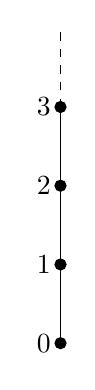
\begin{tikzpicture}
		\filldraw[black] (0,0) circle (2pt) node[anchor=east]{0};
		\filldraw[black] (0,1) circle (2pt) node[anchor=east]{1};
		\filldraw[black] (0,2) circle (2pt) node[anchor=east]{2};
		\filldraw[black] (0,3) circle (2pt) node[anchor=east]{3};
		\draw[black] (0,0)--(0,1);
		\draw[black] (0,1)--(0,2);
		\draw[black] (0,2)--(0,3);
		\draw[dashed,black] (0,3)--(0,4);
	\end{tikzpicture}
\captionof{figure}{Diagramma di Hasse dell'insieme totalmente ordinato $(\mathbb{N},\leq)$}
\end{center}

\begin{example}
	 Si consideri l'insieme $S=\{1,2,3\}$ con la relazione d'ordine usuale. Il diagramma \ref{fig:hasse2} non rappresenta un diagramma di Hasse in quanto $1 \cancel{\lessdot} 3$. Infatti: $] 1,3[ = \{2\} \neq \varnothing$.
	
	\begin{center}
		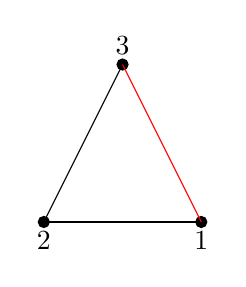
\begin{tikzpicture}
				\filldraw[black] (0,0) circle (2pt) node[anchor=south]{$3$};
				\filldraw[black] (-1,-2) circle (2pt) node[anchor=north]{$2$};
				\filldraw[black] (1,-2) circle (2pt) node[anchor=north]{$1$};
				
				\draw[black] (0,0)--(-1,-2);
				\draw[black] (-1,-2) -- (1,-2);
				\draw[red] (1,-2) -- (0,0);
		\end{tikzpicture}
			\captionof{figure}{}\label{fig:hasse2}
	\end{center}
\end{example}

\begin{example}
	Si consideri l'insieme $S=\{1,2,3\}$ ordinato mediante la relazione identica, o d'uguaglianza $id_{S}$. Chiaramente ogni elemento, essendo diverso da ogni altro elemento dell'insieme, sarà in relazione solo con se stesso. IL diagramma di Hasse che ne deriva prende il nome di \textbf{anticatena}:
	\medskip
	
	\begin{center}
		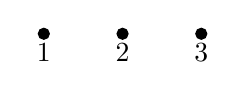
\begin{tikzpicture}
			\filldraw[black] (0,0) circle (2pt) node[anchor=north]{1};
			\filldraw[black] (1,0) circle (2pt) node[anchor=north]{2};
			\filldraw[black] (2,0) circle (2pt) node[anchor=north]{3};
		\end{tikzpicture}
	\end{center}
\end{example}

\begin{example}
	Le classi in \texttt{java.util} ordinate mediante la relazione gerarchica formano un insieme parzialmente ordinato in quanto non tutte le classi sono in relazione tra di loro (ad esempio \texttt{Vector} e \texttt{HashSet}). Si ottiene il seguente diagramma delle classi che non è altro che un diagramma di Hasse dell'insieme ordinato:
	\begin{center}
		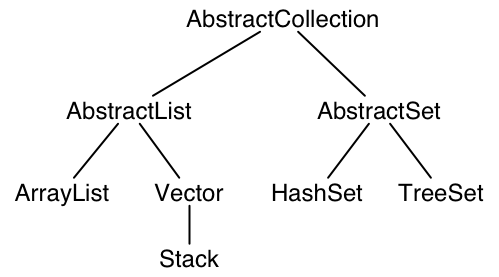
\includegraphics[scale=.35]{res/pojavautil.png}
	\end{center}
\end{example}
\begin{example}
\begin{enumerate}
		\item  Si consideri l'insieme ordinato $(\mathcal{P}(I_{n}), \subseteq)$ nel caso in cui $I_{n}$ sia l'insieme vuoto, $I_{n}$ abbia un solo elemento, due e tre elementi. Ricordiamo che $I_{n} = \{x \in \mathbb{N} \ | \ x \leq n\}$. Si ottengono quindi i diagrammi mostrati in Figura:
	
	\begin{center}
		\begin{minipage}{.1\textwidth}
			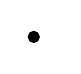
\begin{tikzpicture}
				\filldraw[black] (5,0) circle (2pt) node[anchor=west]{$\varnothing$};
			\end{tikzpicture}
		\end{minipage}
		\begin{minipage}{.1\textwidth}
			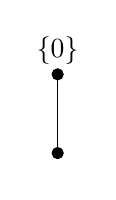
\begin{tikzpicture}
				\filldraw[black] (0,0) circle (2pt) node[anchor=south]{$\{0\}$};
				\filldraw[black] (0,-1) circle (2pt) node[anchor=north]{$\varnothing$};
				\draw[black] (0,0)--(0,-1);
			\end{tikzpicture}
		\end{minipage}
		\begin{minipage}{.25\textwidth}
			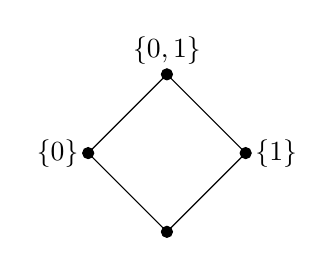
\begin{tikzpicture}
				\filldraw[black] (0,1) circle (2pt) node[anchor=south]{$\{0,1\}$};
				\filldraw[black] (-1,0) circle (2pt) node[anchor=east]{$\{0\}$};
				\filldraw[black] (1,0) circle (2pt) node[anchor=west]{$\{1\}$};
				\filldraw[black] (0,-1) circle (2pt) node[anchor=north]{$\varnothing$};
				
				\draw[black] (0,1)--(-1,0);
				\draw[black] (-1,0) -- (0,-1);
				\draw[black] (0,-1) -- (1,0);
				\draw[black] (1,0) -- (0,1);
			\end{tikzpicture}
		\end{minipage}
		\begin{minipage}{.45\textwidth}
			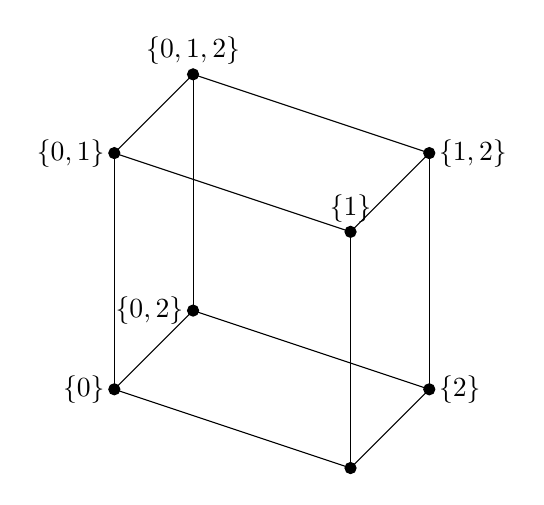
\begin{tikzpicture}
				\filldraw[black] (1,2) circle (2pt)node[anchor=south]{$\{0,1,2\}$};
				\filldraw[black] (0,1) circle (2pt)node[anchor=east]{$\{0,1\}$};
				\filldraw[black] (4,1) circle (2pt)node[anchor=west]{$\{1,2\}$};
				\filldraw[black] (3,0) circle (2pt)node[anchor=south]{$\{1\}$};
				\filldraw[black] (1,-1) circle (2pt)node[anchor=east]{$\{0,2\}$};
				\filldraw[black] (4,-2) circle (2pt)node[anchor=west]{$\{2\}$};
				\filldraw[black] (3,-3) circle (2pt)node[anchor=west]{$\varnothing$};
				\filldraw[black] (0,-2) circle (2pt)node[anchor=east]{$\{0\}$};
				\draw[black] (1,2)--(0,1);
				\draw[black] (0,1) -- (0,-2);
				\draw[black] (1,2) -- (4,1);
				\draw[black] (4,1) -- (4,-2);
				\draw[black] (3,0) -- (4,1);
				\draw[black] (0,1) -- (3,0);
				\draw[black] (0,-2) -- (3,-3);
				\draw[black] (3,-3) -- (4,-2);
				\draw[black] (1,2) -- (1,-1);
				\draw[black] (3,-3) -- (3,0);
				\draw[black] (1,-1) -- (4,-2);
				\draw[black] (0,-2) -- (1,-1);
			\end{tikzpicture}
		\end{minipage}
	\end{center}

\item 	Consideriamo l'insieme $Div(36)=\{1,2,3,4,6,9,12,18,36\}$ ordinato secondo la divisibilità. Il suo diagramma di Hasse è:
	\begin{center}
		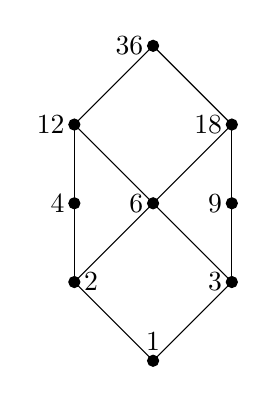
\begin{tikzpicture}
			\filldraw[black] (2,0) circle (2pt)node[anchor=south]{1};
			\filldraw[black] (1,1) circle (2pt)node[anchor=west]{2};
			\filldraw[black] (3,1) circle (2pt)node[anchor=east]{3};
			\filldraw[black] (1,2) circle (2pt)node[anchor=east]{4};
			\filldraw[black] (2,2) circle (2pt)node[anchor=east]{6};
			\filldraw[black] (3,2) circle (2pt)node[anchor=east]{9};
			\filldraw[black] (1,3) circle (2pt)node[anchor=east]{12};
			\filldraw[black] (3,3) circle (2pt)node[anchor=east]{18};
			\filldraw[black] (2,4) circle (2pt)node[anchor=east]{36};
			\draw[black] (2,0)--(1,1);
			\draw[black] (2,0)--(3,1);
			\draw[black] (1,1)--(1,2);
			\draw[black] (1,1)--(2,2);
			\draw[black] (3,1)--(2,2);
			\draw[black] (3,1)--(3,2);
			\draw[black] (2,2)--(1,3);
			\draw[black] (2,2)--(3,3);
			\draw[black] (1,2)--(1,3);
			\draw[black] (3,2)--(3,3);
			\draw[black] (1,3)--(2,4);
			\draw[black] (3,3)--(2,4);
		\end{tikzpicture}
	\end{center}
\end{enumerate}
\end{example}



\begin{osservation}
	Due insiemi si dicono \textbf{isomorfi} se hanno lo stesso diagramma di Hasse. Il duale di un diagramma di Hasse (ovvero il diagramma di Hasse della sua relazione opposta) si ottiene ruotando il grafico di 180°.
\end{osservation}

\begin{example}
	Consideriamo l'insieme ordinato $(\mathbb{N},\divides)$ e costruiamone il diagramma di Hasse (parziale):
	\begin{center}
		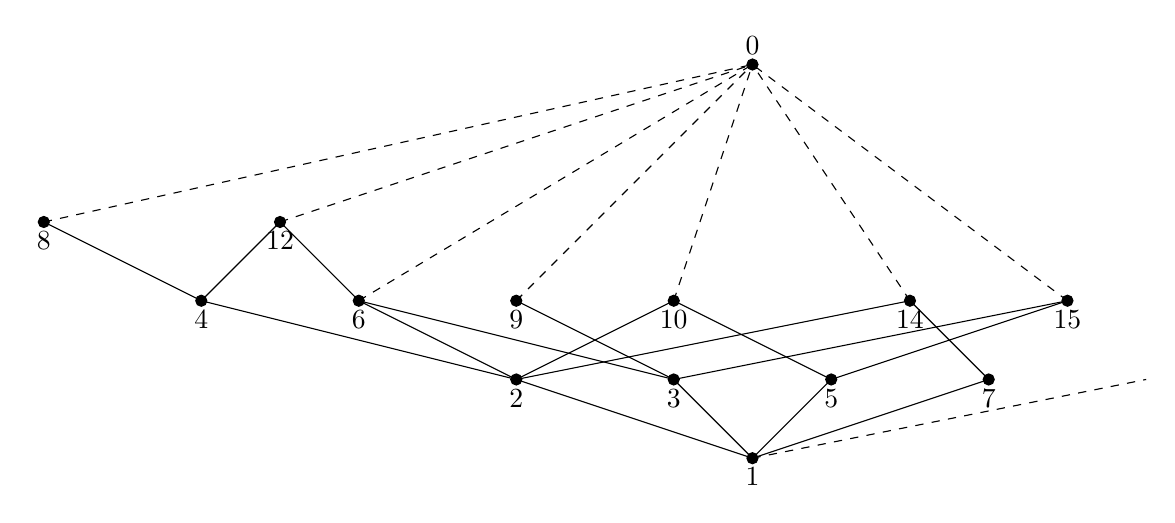
\begin{tikzpicture}
			\filldraw[black] (0,0) circle (2pt)node[anchor=north]{1};
			\filldraw[black] (-3,1) circle (2pt)node[anchor=north]{2};
			\filldraw[black] (-1,1) circle (2pt)node[anchor=north]{3};
			\filldraw[black] (1,1) circle (2pt)node[anchor=north]{5};
			\filldraw[black] (3,1) circle (2pt)node[anchor=north]{7};
			\draw[black] (0,0)--(-3,1);
			\draw[black] (0,0)--(-1,1);
			\draw[black] (0,0)--(1,1);
			\draw[black] (0,0)--(3,1);
			\draw[dashed] (0,0)--(5,1);
			\filldraw[black] (-7,2) circle (2pt)node[anchor=north]{4};
			\filldraw[black] (-5,2) circle (2pt)node[anchor=north]{6};
			\filldraw[black] (-3,2) circle (2pt)node[anchor=north]{9};
			\filldraw[black] (-1,2) circle (2pt)node[anchor=north]{10};
			\filldraw[black] (2,2) circle (2pt)node[anchor=north]{14};
			\filldraw[black] (4,2) circle (2pt)node[anchor=north]{15};
			\draw[black] (-3,1) --(-7,2);
			\draw[black] (-3,1) --(-5,2);
			\draw[black] (-3,1) --(-1,2);
			\draw[black] (-3,1) --(2,2);
			\draw[black] (-1,1)--(-5,2);
			\draw[black] (-1,1)--(-3,2);
			\draw[black] (-1,1)--(4,2);
			\draw[black] (1,1)--(-1,2);
			\draw[black] (1,1)--(4,2);
			\draw[black] (3,1)--(2,2);
			\filldraw[black] (-9,3) circle(2pt) node[anchor=north]{8};
			\filldraw[black] (-6,3) circle(2pt) node[anchor=north]{12};
			\draw[black] (-7,2)--(-9,3);
			\draw[black] (-7,2)--(-6,3);
			\draw[black] (-5,2)--(-6,3);
			\filldraw[black] (0,5) circle (2pt) node[anchor=south]{0};
			\draw[dashed](-9,3)--(0,5);
			\draw[dashed](-6,3)--(0,5);
			\draw[dashed](-5,2)--(0,5);
			\draw[dashed](-3,2)--(0,5);
			\draw[dashed](-1,2)--(0,5);
			\draw[dashed](2,2)--(0,5);
			\draw[dashed](4,2)--(0,5);
		\end{tikzpicture}
	\captionof{figure}{Diagramma di Hasse dell'insieme ordinato $(\mathbb{N},\divides)$.}\label{fig:hasse_n_divides}
	\end{center}
\end{example}

\subsection{Maggioranti, minoranti, estremo superiore ed inferiore}

\begin{defbox}{Maggioranti e minoranti}
	Sia $(S, \leq)$ un insieme ordinato, e sia $X$ una parte non vuota di $S$. Un elemento $a \in S$ si dice \textbf{minorante} di $X$ se risulta $a \leq x$ per ogni $x$ in $X$. Si dice invece che $a$ è un \textbf{maggiorante} di $X$ se $x \leq a$ per ogni $x \in X$.
\end{defbox}

\begin{defbox}{Insiemi inferiormente e superiormente limitati}
	Una parte $X\subseteq S$ si dice \textbf{inferiormente limitata} se è dotata di minoranti, mentre $X$ si dice \textbf{superiormente limitata} se è dotata di maggioranti.
\end{defbox} 

L'insieme dei minoranti di $X$ si denota col simbolo:
\begin{equation}
	X^{\downarrow}_{(S,\leq)}=\{a \in S \ | \ \forall x \in X (a \leq x)\}
\end{equation}
Mentre l'insieme dei maggioranti si denota col simbolo:
\begin{equation}
	X^{\uparrow}_{(S,\leq)}=\{a \in S \ | \ \forall x \in X (x \leq a)\}
\end{equation}


\begin{example}
	Si consideri il seguente diagramma di Hasse:
	\begin{center}
		\begin{tikzpicture}
			\filldraw[black] (1,1) circle (2pt) node[anchor=east]{c};
			\filldraw[black] (0,0) circle (2pt) node[anchor=east]{d};
			\filldraw[black] (2,0) circle (2pt) node[anchor=east]{e};
			\filldraw[black] (0,-2) circle (2pt) node[anchor=east]{a};
			\filldraw[black] (2,-2) circle (2pt)node[anchor=west]{b};
			\filldraw[black](1,-3) circle (2pt)node[anchor=north]{f};
			\filldraw[black](3,-1) circle (2pt)node[anchor=east]{g};
			\node[shape=ellipse,minimum height=1cm,draw=blue,fit={(0,-2)(2,-2)}]{};
			\draw[black] (1,1)--(0,0);
			\draw[black] (1,1)--(2,0);
			\draw[black] (2,0)--(0,-2);
			\draw[black] (0,0)--(0,-2);
			\draw[black] (0,-2)--(1,-3);
			\draw[black] (1,-3)--(3,-1);
			\draw[black] (2,-2)--(1,-3);
			\draw[black] (2,0)--(2,-2);
		\end{tikzpicture}
	\end{center}
	Si ha che l'insieme dei maggioranti di $\{a,b\}$ è dato da:
	\begin{displaymath}
		\{a,b\}^{\uparrow} =\{c,e\}
	\end{displaymath}
	mentre l'insieme dei minoranti di $\{a,b\}$ è:
	\begin{displaymath}
		\{a,b\}^{\downarrow} = \{f\}
	\end{displaymath}
\end{example}

\begin{example}
	Sia $(\mathcal{P}(S),\subseteq)$ allora, per un sottoinsieme $X \subseteq S$:
	\begin{eqnarray}
			X^{\uparrow} &= \{ Y \in \mathcal{P}(S) \; | \; \forall c \in \bigcup X (c \in Y) \} = \{Y \in \mathcal{P}(S) \; | \; \bigcup X \subseteq Y \}\\
			X^{\downarrow} &= \{Y \in \mathcal{P}(S) \; | \; \forall x \in X (Y \subseteq x )\} = \begin{cases}
				\{Y \in \mathcal{P}(S) \; | \; Y \subseteq \bigcap X\} & \text{se $X \neq \emptyset$}\\
				\{Y \; | \; Y \in \mathcal{P}(S) \} = \mathcal{P}(S) & \text{se $X= \emptyset$}
			\end{cases}
	\end{eqnarray}
Sia $S= \mathbb{N}$ e sia $X= \{\{1,2\},\{2,3\}\}$. Allora:
\begin{align*}
	X^{\uparrow} &=& \{Y \in \mathcal{P}(\mathbb{N}) \; | \; \bigcup X \subseteq Y \} = \{Y 	\in \mathcal{P}(\mathbb{N}) \; | \; \{1,2,3\} \subseteq Y \}\\
	X^{\downarrow} &=& \{Y \in \mathcal{P}(\mathbb{N})\; | \; Y \subseteq \bigcap X\} = \{Y \in \mathcal{P}(\mathbb{N}) \; | \; Y \subseteq \{2\} \} = \{\emptyset, \{2\}\}
\end{align*}
\end{example}

\begin{defbox}{Estremo inferiore e superiore}
	Sia $(S,\leq)$ un insieme ordinato, e sia $X$ una parte inferiormente limitata di $S$. Allora l'insieme dei minoranti di $X$ è una parte non vuota di $S$, il cui eventuale massimo di chiama \textbf{estremo inferiore} di $X$ e si denota col simbolo $inf_{(S,\leq)} X$. Se invece $X$ è una parte superiormente limitata di $S$, l'eventuale minimo dell'insieme dei maggioranti di $X$ si chiama \textbf{estremo superiore} di $X$ e si denota col simbolo $sup_{(S,\leq)} X$:
	\begin{eqnarray}
		inf_{(S,\leq)} X = max(X^{\downarrow}_{(S,\leq)})\\
		sup_{(S,\leq)} X = min(X^{\uparrow}_{(S,\leq)})
	\end{eqnarray}
\end{defbox}

\begin{example}
	Sia $X = \{C \in \mathcal{P}(\{1,2,3,4,5,6\}) \; | \; |C| \text{ è pari} \}$, ordinato mediante l'inclusione. Sia $A = \{\{1,2\},\{1,3\},\{2,5\}\} \subseteq X$. Allora abbiamo $A^{\downarrow} = \{\emptyset\}	$ e $A^{\uparrow}=\{\{1,2,3,5\},\{1,2,3,4,5,6\}\}
	$. Dunque:
\begin{align*}
	inf(A) &= max(A^{\downarrow}) = \emptyset\\
	sup(A) &= min(A^{\uparrow}) = \{1,2,3,5\}
\end{align*}
\end{example}

\begin{osservation}
	Se $S$ è un insieme ordinato non costituito da un solo elemento, nell'insieme ordinato $(\mathcal{P}(S)\setminus\{\varnothing\}, \subseteq)$ gli elementi minimali sono i sottoinsiemi del tipo $\{x\}$, con $x \in S$. Similmente, è chiaro che se l'insieme ordinato $S$ è dotato di massimo, questo è \textit{l'unico elemento massimale}. D'altra parte, qualunque sia l'insieme $S$ non costituito da un solo elemento, per ogni $x \in S$ il sottoinsieme $S \setminus \{x\}$ è un elemento massimale dell'insieme ordinato $(\mathcal{P}(S)\setminus \{S\}, \subseteq)$.
\end{osservation}

\begin{teorbox}
	Sono equivalenti le seguenti affermazioni:
	\begin{enumerate}
		\item $a \leq b$
		\item $a = min \{a,b\}$
		\item $a = inf\{a,b\}$
		\item $a \in \{a,b\}^{\downarrow}$
	\end{enumerate}
\end{teorbox}

\begin{osservation}
	Riprendiamo il Diagramma di Hasse dell'insieme ordinato $(\mathbb{N},\divides)$ (Figura \ref{fig:hasse_n_divides}). Per ogni coppia $(a,b)$ vale:
	\begin{eqnarray}
		inf(\{a,b\}) = MCD(a,b) \\
		sup(\{a,b\}) = mcm(a,b)
	\end{eqnarray}
Infatti, il massimo comun divisore di $a$ e $b$ è il più grande numero che divide $a$ e $b$, ovvero risulta essere il massimo dei minoranti secondo la relazione di divisibilità. Analogamente, il minimo comune multiplo risulta essere il minimo dell'insieme dei maggioranti (i multipli comuni di $a$ e $b$ per l'appunto).
\end{osservation}

\begin{example}
	Sia $(A,\leq)$ l'insieme ordinato definito dal diagramma di Hasse mostrato in Figura \ref{fig:example_inf_sup} e sia $B=\{c,d,e\}$:
	\begin{center}
		\begin{tikzpicture}
			\filldraw[black] (.5,2.5)circle (2pt) node[anchor=south]{a};
			\filldraw[black] (4,2.5) circle (2pt) node[anchor=south]{b};
			\filldraw[black] (2,1.5) circle (2pt) node[anchor=south]{c};
			\filldraw[black] (1,1) circle (2pt) node[anchor=south]{d};
			\filldraw[black] (3,1) circle (2pt) node[anchor=south]{e};
			\filldraw[black] (2,0) circle (2pt) node[anchor=south]{f};
			\filldraw[black] (4.5,.5) circle (2pt) node[anchor=south]{g};
			\node[shape=ellipse,draw=blue,fit={(2,1.5)(1,1)(3,1)}]{};
			\draw[black,thin] (2,0)--(1,1);
			\draw[black,thin] (2,0)--(3,1);
			\draw[black,thin] (4.5,.5)--(3,1);
			\draw[black,thin] (1,1)--(2,1.5);
			\draw[black,thin] (2,1.5)--(3,1);
			\draw[black,thin] (2,1.5)--(.5,2.5);
			\draw[black,thin] (2,1.5)--(4,2.5);
		\end{tikzpicture}
		\captionof{figure}{}\label{fig:example_inf_sup}
	\end{center}
	L'insieme dei maggioranti di $B$ è: $$B^{\uparrow} = \{a,b,c\}$$ e risulta $sup \ B = c$ poiché $c \in B$, $c$ è l'elemento massimo di $B$. L'insieme dei minoranti di $B$ è $ \{ f \} $ e quindi $inf \ B = f$ . Poiché $f \notin B$ allora non esiste il minimo di $B$. Osserviamo che $g$ non precede $d$ e quindi non è un minorante di $B$.
\end{example}

\begin{example}
	Sia $(A,\leq)$ l'insieme ordinato definito dal diagramma di Hasse in Figura \ref{fig:example_inf_sup2} e sia $B = \{d,e,f\}$. L'insieme dei maggioranti di $B$ è $$B^{\uparrow}=\{a,b,c\}$$ e risulta sup \ B = c. Poiché $c \notin B$ allora il massimo di $B$ non esiste. L'insieme dei minoranti di $B$ è $$B^{\downarrow} = \{f,h\} $$ e risulta $inf \ B = f$. Poiché $f \in B$, $f$ è l'elemento minimo di $B$ (osserviamo che $g$ non è un minorante di $B$.
	\begin{center}
		\begin{tikzpicture}
			\filldraw[black] (1,4)circle (2pt) node[anchor=south]{a};
			\filldraw[black] (3,4) circle (2pt) node[anchor=south]{b};
			\filldraw[black] (2,3) circle (2pt) node[anchor=south]{c};
			\filldraw[black] (1,2) circle (2pt) node[anchor=south]{d};
			\filldraw[black] (3,2) circle (2pt) node[anchor=south]{e};
			\filldraw[black] (2,1) circle (2pt) node[anchor=south]{f};
			\filldraw[black] (4,1) circle (2pt) node[anchor=south]{g};
			\filldraw[black](3,0) circle (2pt) node[anchor=south]{h};
			\node[shape=ellipse,draw=blue,fit={(3,2)(1,2)(2,1)}]{};
			\draw[black,thin](3,0)--(2,1);
			\draw[black,thin](3,0)--(4,1);
			\draw[black,thin](4,1)--(3,2);
			\draw[black,thin](3,2)--(2,3);
			\draw[black,thin](2,3)--(1,4);
			\draw[black,thin](3,0)--(2,1);
			\draw[black,thin](2,1)--(1,2);
			\draw[black,thin](1,2)--(2,3)--(3,4);
			\draw[black,thin](2,1)--(3,2);
		\end{tikzpicture}
		\captionof{figure}{}\label{fig:example_inf_sup2}
	\end{center}
\end{example}

\begin{example}
 Sia $(A,\leq)$ l'insieme ordinato definito dal diagramma di Hasse in Figura \ref{fig:example_inf_sup3} e sia $B=\{b,c,d\}$. L'insieme dei maggioranti di $B$ è $$B^{\uparrow}=\{a,b\}$$ e risulta $sup \ B = b$. Poiché $b \in B$, $b$ è il massimo di $B$. L'insieme dei minoranti di $B$ è $B^{\downarrow}=\{e,f\}$ Poiché gli elementi $e,f$ sono non confrontabili, $inf \ B$ non esiste.
	\begin{center}
		\begin{tikzpicture}
			\filldraw[black] (2.5,4)circle (2pt) node[anchor=south]{a};
			\filldraw[black] (2.5,3) circle (2pt) node[anchor=north]{b};
			\filldraw[black] (0,2) circle (2pt) node[anchor=south]{c};
			\filldraw[black] (5,2) circle (2pt) node[anchor=south]{d};
			\filldraw[black] (1,0) circle (2pt) node[anchor=north]{e};
			\filldraw[black] (4,0) circle (2pt) node[anchor=north]{f};
			\node[shape=ellipse,draw=blue,fit={(2.5,3)(0,2)(5,2)}]{};
			\draw[black](1,0)--(5,2)--(2.5,3)--(2.5,4);
			\draw[black](4,0)--(0,2)--(2.5,3);
			\draw[black]  (0,2)--(1,0);
			\draw[black]  (5,2)--(4,0);
		\end{tikzpicture}
		\captionof{figure}{}\label{fig:example_inf_sup3}
	\end{center}
\end{example}
\section{Reticoli}

\begin{defbox}{Reticolo}
	Sia $(S, \leq)$ un insieme parzialmente ordinato. $S$ si dice \textbf{reticolo} se e solo se:
	\begin{equation}
		\forall a,b \in S \bigl( \exists inf_{(S,\leq)}(\{a,b\}) \land \exists sup_{(S,\leq)}(\{a,b\})
	\end{equation}
\end{defbox}

\begin{example}
\begin{enumerate}
	\item Si consideri il seguente diagramma di Hasse:
	\begin{center}
		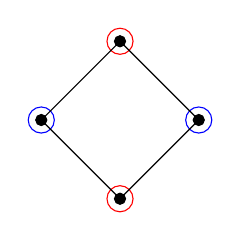
\begin{tikzpicture}
			\filldraw[black] (1,1) circle (2pt) node[shape = circle, minimum size=3pt, red, draw]{};
			\filldraw[black] (2,0) circle (2pt) node[shape = circle, blue, minimum size = 3pt, draw]{};
			\filldraw[black] (0,0) circle (2pt) node[shape = circle, blue, minimum size = 3pt, draw]{};
			\filldraw[black] (1,-1) circle (2pt) node[shape = circle, red, minimum size = 3pt, draw]{};
			\draw[black, thin] (1,1) -- (2,0)--(1,-1)--(0,0)--(1,1);
		\end{tikzpicture}
	\end{center}
	Per verificare che tale diagramma rappresenti un reticolo basterà osservare che le coppie non confrontabili (evidenziate in blu) abbiano sia un estremo superiore che un estremo inferiore (evidenziati in rosso).
	\item L'insieme dei numeri naturali, $\mathbb{N}$, ordinato mediante la divisibilità, è un reticolo.
	\item L'insieme $\{1,2,3,4,5,6,7,8,9\}$, ordinato mediante la divisibilità, non è un reticolo. Infatti, per esempio, $sup(\{6,9\})$ non esiste.
	\begin{center}
		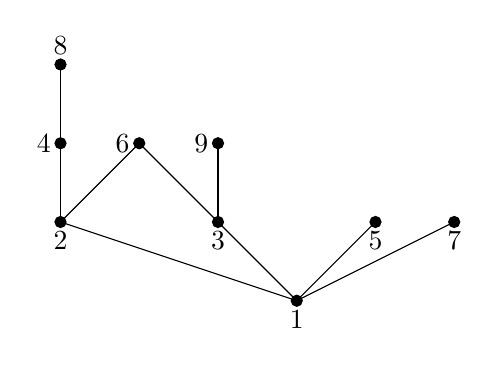
\begin{tikzpicture}
			\filldraw[black] (0,0) circle (2pt)node[anchor=north]{1};
			\filldraw[black] (-3,1) circle (2pt)node[anchor=north]{2};
			\filldraw[black] (-1,1) circle (2pt)node[anchor=north]{3};
			\filldraw[black] (-3,2) circle (2pt)node[anchor=east]{4};
			\filldraw[black] (1,1) circle (2pt)node[anchor=north]{5};
			\filldraw[black] (-2,2) circle (2pt)node[anchor=east]{6};
			\filldraw[black] (2,1) circle (2pt)node[anchor=north]{7};
			\filldraw[black] (-3,3) circle (2pt)node[anchor=south]{8};
			\filldraw[black] (-1,2) circle (2pt)node[anchor=east]{9};
			\draw[black] (0,0)--(-3,1);
			\draw[black] (0,0)--(-1,1);
			\draw[black] (0,0)--(1,1);
			\draw[black] (0,0)--(2,1);
			\draw[black] (-3,1)--(-2,2);
			\draw[black] (-3,1)--(-3,2);
			\draw[black] (-3,2)--(-3,3);
			\draw[black] (-1,1)--(-1,2);
			\draw[black] (-1,1)--(-2,2);
		\end{tikzpicture}
	\end{center}
	\item L'insieme $Div(36) = \{1,2,3,4,6,9,12,18,36\}$, ordinato mediante la divisibilità, è un reticolo. 
\end{enumerate}
\end{example}



\begin{propbox}
	Sia $(S,\leq)$ un reticolo e consideriamo $a \in S$. L'elemento $a$ è minimale in $S$ se e soltanto se $a = min(S,\leq)$. Dualmente per gli elementi massimali.
\end{propbox}

\begin{proof}
	\begin{itemize}
		\item[$\impliedby$] La condizione è chiaramente sufficiente. 
		\item[$\implies$] Sia $a$ un elemento minimale. Per ogni $b \in S$ poniamo $X = \{a,b\}$ e sia $c = inf (X) = max (X^{\downarrow})$, allora $c  \leq  a $ e $c \leq b$. Tuttavia, essendo $a$ minimale deve essere $c=a$ e quindi $a \leq b$ per ogni $b \in S$. Quindi, per definizione di minimo si ha l'asserto.
	\end{itemize}
\end{proof}

\begin{osservation}\label{oss:min_inf}
	Per ogni $a,b \in (S,\leq)\bigl( a \leq b \iff a = inf\{a,b\} \iff b= sup \{a,b\} \bigr)$. Inoltre, se $X \subseteq S$ ed esiste $x= inf(X)$ allora, essendo l'estremo inferiore il massimo dei minoranti, vale: $X^{\downarrow} = \{x\}^{\downarrow}$.
\end{osservation}

\begin{defbox}{Reticolo limitato e completo}
	Un reticolo si dice \textbf{limitato} se ammette minimo e massimo. Un reticolo si dice \textbf{completo} se ogni sua parte non vuota è dotata di estremo inferiore e superiore. Ogni reticolo completo è anche limitato.
\end{defbox}

\begin{osservation}
	Un reticolo finito non vuoto è sempre limitato. Il viceversa non vale: ci sono dei reticoli infiniti che sono limitati. Ad esempio se $A$ è un insieme infinito, $\mathcal{P}(A)$ è limitato, infatti si ha che il massimo di $\mathcal{P}(A)$ è $A$ stesso mentre il minimo è rappresentato dall'insieme vuoto. Il reticolo $(\mathbb{N},\leq)$ ha minimo, il numero naturale 0, ma non ha massimo. Quindi non è un reticolo limitato.
\end{osservation}


\begin{propbox}\label{prop_demorgan_minimali}
	Sia $(S,\rho)$ un insieme ordinato e siano $X,Y \subseteq S$ delle parti finite di $S$. Supponiamo che esistano $x= inf (X)$ e $y=inf(Y)$. Allora:
	\begin{align*}
		(X \cup Y )^{\downarrow} = X^{\downarrow} \cap Y^{\downarrow} = \{x\}^{\downarrow} \cap \{y\}^{\downarrow}
	\end{align*}
	Per dualità vale l'analogo per i maggioranti. Inoltre, se $(S,\rho)$ è un reticolo esiste $a=inf (\{x,y\}) = max(\{x,y\}^{\downarrow}) = max\bigl((X \cup Y)^{\downarrow}\bigr) = inf(X \cup Y)$.
\end{propbox}
\begin{proof}
	Sia $x \in (X \cup Y)^{\downarrow}$, valgono allora le seguenti equivalenze:
	\begin{align*}
		x \in (X \cup Y)^{\downarrow} &\iff \forall y \in X \cup Y (x\leq y) \\
		&\iff \forall y \bigl( (y \in X \lor y \in Y) \implies (x \leq y) \bigr) \\
		&\iff \forall y (y \in X \implies x \leq y) \land \forall y (y \in Y \implies x \leq y)\\
		&\iff x \in X^{\downarrow} \land x \in Y^{\downarrow}\\
		&\iff x \in X^{\downarrow} \cap Y^{\downarrow}
	\end{align*}
\end{proof}
\begin{corolbox}\label{corol:inf_sup}
	Sia $(S,\leq)$ un reticolo. Ogni sua parte finita è dotata di estremo inferiore e superiore.
\end{corolbox}
\begin{proof}
	Consideriamo una parte finita $T =\{a_{1},a_{2},\ldots,a_{n}\} \subset S$ e procediamo per induzione.
	\begin{itemize}
		\item Se $n=1$, cioè $T=\{a_{1}\}$, l'estremo inferiore di $T$ è semplicemente $a_{1}$ perché, per l'Osservazione \ref{oss:min_inf} si ha $T^{\downarrow}=\{a_{1}\}^{\downarrow}$, allora:
		\begin{align*}
			 inf(T)=max(T^{\downarrow}) = max(\{a_{1}\}^{\downarrow})=a_{1}
		\end{align*}
		\item Supponiamo che l'estremo inferiore esista per tutti i sottoinsiemi finiti di $S$ con $n$ elementi. Consideriamo un sottoinsieme con $n+1$ elementi, $T=\{a_{1},a_{2},\ldots,a_{n+1}\}$. Possiamo riscrivere $T$ come l'unione dell'insieme $T_{1}=\{a_{1},\ldots,a_{n}\}$ e $T_{2}=\{a_{1}\}$:
		\begin{align*}
			T = T_{1} \cup T_{2}
		\end{align*}
		Per ipotesi induttiva esiste l'estremo inferiore di $T_{1}$, sia esso $b = inf(\{a_{1},a_{2},\ldots,a_{n}\})$ ed, essendo $T_{2}$ un insieme di un solo elemento, risulta inoltre $inf(T_{2}) = a_{n+1}$. Per la Proposizione \ref{prop_demorgan_minimali} vale allora:
		\begin{align*}
			T^{\downarrow} &= (T_{1} \cup T_{2})^{\downarrow} \\
			&=T_{1}^{\downarrow} \cap T_{2}^{\downarrow} \\
			&= \{b\}^{\downarrow} \cap \{a_{n+1}\}^{\downarrow} \\
			&= \{b,a_{n+1}\}^{\downarrow}
		\end{align*}
	Dato che $S$ è un reticolo, l'insieme $\{b,a_{n+1}\}$ sicuramente ammette estremo inferiore, e vale quindi:
	\begin{displaymath}
		inf(\{b,a_{n+1}\}) = max(\{b,a_{n+1}\}^{\downarrow}) = max(T^{\downarrow}) = inf(T)
	\end{displaymath}
	\end{itemize}
\end{proof}

Se un insieme finito è un reticolo allora risulta essere un reticolo completo.

\subsection{Operazioni reticolari}
In questa sezione vedremo che i reticoli possono essere definiti, in modo equivalente, come insiemi muniti di due operazioni che soddisfano certe proprietà. L'idea è che $(a,b) \mapsto sup(\{a,b\})$ e $(a,b) \mapsto inf(\{a,b\})$ sono due operazioni che possiamo denotare rispettivamente $a \vee b$ e $a \wedge b$. Viceversa, la relazione d'ordine può essere ricavata da queste operazioni, nel modo seguente:
\begin{align*}
	\forall a,b \in S \bigl(	a \ \rho \ b \iff b = a \vee b 	\bigr)
\end{align*}
oppure:
\begin{align*}
	\forall a,b \in S \bigl(	a \ \rho \ b \iff a = a \wedge b 	\bigr)
\end{align*}

\begin{propbox}
	Sia $S$ un reticolo. Allora posto $a \vee b = sup(\{a,b\})$ e $a \wedge b = inf(\{a,b\})$, si ha che le operazioni su $S$:
	\begin{eqnarray}
		(a,b) \mapsto a \vee b \\
		(a,b) \mapsto a \wedge b	
	\end{eqnarray}
verificano le seguenti proprietà:
\begin{enumerate}
	\item \textit{Commutatività:} $a \vee b = b \vee a$ e $a \wedge b = b \wedge a$, per ogni $a,b \in S$;
	\item \textit{Associatività:} $a \vee (b \vee c) = (a \vee b) \vee c$ e $a \wedge (b \wedge c) = (a \wedge b) \wedge c$ per ogni $a,b,c \in S$
	\item \textit{Assorbimento:} $a \wedge ( a \vee b) = a$, $a \vee (a \wedge b) = a$, per ogni $a,b \in S$.
\end{enumerate}
\end{propbox}
\begin{proof}
	Evidente, la prova è lasciata al lettore come esercizio.
\end{proof}
\begin{osservation}
	Per ogni $a \in S$, $a$ è neutro rispetto a $\vee$ se e soltanto se, per ogni $b \in S$ si ha $b = a \vee b$. Cioè, se e soltanto se, $\forall b \in S (a \leq b)$ e cioè, $a = min(S,\leq)$. Dualmente, un elemento $a$ è neutro rispetto a $\vee$ se è il massimo di $(S,\leq)$. L'eventuale minimo di un reticolo si indica con il simbolo $0$ mentre l'eventuale massimo si indica con il simbolo 1.
\end{osservation}

Esaminiamo ora il viceversa della precedente Proposizione.
\begin{propbox}
	Sia $(S,\vee,\wedge)$ un insieme munito di due operazioni che verificano le proprietà:
	\begin{enumerate}
		\item \textit{Commutatività:} $a \vee b = b \vee a$ e $a \wedge b = b \wedge a$, per ogni $a,b \in S$;
		\item \textit{Associatività:} $a \vee (b \vee c) = (a \vee b) \vee c$ e $a \wedge (b \wedge c) = (a \wedge b) \wedge c$ per ogni $a,b,c \in S$
		\item \textit{Assorbimento:} $a \wedge ( a \vee b) = a$, $a \vee (a \wedge b) = a$, per ogni $a,b \in S$.
	\end{enumerate}
Allora la relazione $\rho$ su $S$ definita come:
\begin{equation}
	a \ \rho \ b \iff b = a \vee b
\end{equation}
è una relazione d'ordine su $S$. Si ha anche:
\begin{equation}\label{eq:wedge}
	a \ \rho \ b \iff a = a \wedge b
\end{equation}
Inoltre, $S$, munito di tale relazione d'ordine, è un reticolo, e, per ogni $a,b \in S$:
\begin{align*}
	\begin{cases*}
		sup(\{a,b\}) = a \vee b \\
		inf(\{a,b\}) = a \wedge b \\
	\end{cases*}
\end{align*}
\end{propbox}
\begin{proof}
	Iniziamo con il dimostrare la \ref{eq:wedge}. Infatti, se $a \ \rho \ b$, cioè se $b = a \vee b$, allora per l'assorbimento, $a \wedge b = a \wedge (a \vee b) = a$. Viceversa, se $a = a \wedge b$, ancora per l'assorbimento e per la commutatività, $a \vee b = (a \wedge b) \vee b = b \vee (a \wedge b) = b$.
	
	Dimostriamo ora che $\rho$ è una relazione d'ordine:
	\begin{enumerate}
		\item \textit{Riflessività:} $a \ \rho \ a$, cioè $a = a \vee a$. Infatti, usando le due proprietà di assorbimento, per ogni $a,b \in S$ si ha che $a = a \vee (a \wedge (a \vee b)) = a \vee a$;
		\item \textit{Antisimmetria:} Se $a \ \rho \ b$ e $b \ \rho \ a$, cioè se $b = a \vee b$ e $a = b \vee a $, allora, per la commutatività di $\vee$, deve essere $a=b$;
		\item \textit{Transitività:} se $a \ \rho \ b$ e $b \ \rho \ c$, cioè se $b= a \vee b$ e $c = b \vee c$ segue che $a \vee c = a \vee (b \vee c ) = (a \vee b) \vee c = a \vee c$.
	\end{enumerate}
	
	Rimane da dimostrare l'ultima asserzione. Dimostriamo che:
	\begin{align*}
		a \vee b = sup(\{a,b\})
	\end{align*}
Infatti, $a \ \rho \ (a \vee b)$, perché per la \ref{eq:wedge}, ciò è equivalente al fatto che $a \wedge ( a \vee b) = a$, cosa che è verificata per l'assorbimento. Allo stesso modo, si vede che $b \ \rho (a \vee b)$. Quindi $a \vee b$ è un maggiorante dell'insieme $\{a,b\}$ Rimane da dimostrare che è il minimo dell'insieme dei maggioranti. Supponiamo dunque che $a \ \rho \ c$ e $b \ \rho \ c$, cioè $c = a \vee c = b \vee c$. Allora $(a \vee b) \vee c = a \vee ( b \vee c) = a \vee c = c$, Dunque $(a \vee c) \ \rho \ c$ e l'asserzione è dimostrata. Il fatto che $ a \wedge b = inf(\{a,b\})$ si dimostra in modo analogo.
\end{proof}
\begin{defbox}{Reticolo come algebra}
Una struttura algebrica $(S,\wedge, \vee)$ a due operazioni interne si dice \textbf{reticolo} se le operazioni $\vee$ e $\wedge$ sono associative, commutative, e inoltre per ogni coppia $(a,b)$ di elementi di $S$ risulta:
\begin{eqnarray}\label{eq:assorbimento_meet_join}
	a \wedge(a \vee b) = a\\
	a \vee (a \wedge b)  = a
\end{eqnarray}
ovvero valgono le leggi di assorbimento. Se $(S,\wedge, \vee)$ è un reticolo, le operazioni $\wedge$ e $\vee$ sono spesso chiamate \textbf{intersezione} e \textbf{unione} in $S$ oppure \textbf{meet} e \textbf{join}.
\end{defbox}

\begin{example}
	Sia $X$ un qualunque insieme, e nell'insieme $\mathcal{P}(X)$ delle parti di $X$ si considerino le operazioni:
	\begin{align*}
		\cap: (A,B) \in \mathcal{P}(X)^{2} \mapsto A \cap B \in \mathcal{P}(X)
	\end{align*}
	e:
	\begin{align*}
		\cup: (A,B) \in \mathcal{P}(X)^{2} \mapsto A \cup B \in \mathcal{P}(X)
	\end{align*}
	Allora la terna $(\mathcal{P}(X),\cap,\cup)$ è un reticolo, chiamato \textbf{reticolo delle parti} di $X$.
\end{example}


\subsection{Sottoreticoli}
\begin{defbox}{Sottoreticolo}
	Sia $(S,\leq)$ un reticolo. Una parte $T \subseteq S$ si dice un \textbf{sottoreticolo} se esso è stabile rispetto a ciascuna delle operazioni reticolari $\wedge$ e $\vee$.
\end{defbox}

\begin{propbox}
	Gli intervalli chiusi di un reticolo sono sempre sottoreticoli.
\end{propbox}

\begin{proof}
	La dimostrazione è lasciata al lettore.
\end{proof}
È chiaro che un sottoreticolo è esso stesso un reticolo. Invece il viceversa non è necessariamente vero:  dato un reticolo $S$, esso può avere sottoinsiemi che sono reticoli rispetto alle operazioni di $S$ ma non sono sottoreticoli di $S$.
\begin{example}
	 Si consideri l'insieme $Div(12)=\{1,2,3,4,6,12\}$. Oltre ai \textbf{sottoreticoli banali} ($Div(12)$ stesso e i sottoinsiemi con un solo elemento) abbiamo i sottoreticoli $\{1,2,3,6\}$ e $\{2,4,6,12\}$. Sia $T=Div(12) \setminus \{2\} = \{1,3,4,6,12\} \subset Div(12)$.

	\begin{center}
		\begin{minipage}{.45\textwidth}
			\centering
			\begin{tikzpicture}
				\filldraw[black] (2,0) circle (2pt) node[anchor=north]{1};
				\filldraw[black] (0,1) circle (2pt) node[anchor=east]{3};
				\filldraw[black] (2,2) circle (2pt) node[anchor=south]{6};
				\filldraw[black] (4,1) circle (2pt) node[anchor=south]{2};
				\filldraw[black] (4,3) circle (2pt) node[anchor=south]{12};
				\filldraw[black] (6,2) circle (2pt) node[anchor=west]{4};
				\draw[black,thin] (2,0)--(0,1)--(2,2)--(4,1)--(6,2)--(4,3)--(2,2);
				\draw[black,thin] (2,0) --(4,1);
			\end{tikzpicture}
			\captionof{figure}{Il reticolo $(Div(12), \divides)$}
		\end{minipage}
		\hfil
		\begin{minipage}{.45\textwidth}
			\centering
			\begin{tikzpicture}
				\filldraw[black] (2,0) circle (2pt) node[anchor=north]{1};
				\filldraw[black] (0,1) circle (2pt) node[anchor=east]{3};
				\filldraw[black] (2,2) circle (2pt) node[anchor=south]{6};
				\filldraw[black] (4,3) circle (2pt) node[anchor=south]{12};
				\filldraw[black] (6,2) circle (2pt) node[anchor=west]{4};
				\draw[black,thin] (2,0)--(6,2)--(4,3)--(2,2)--(0,1)--(2,0);
			\end{tikzpicture}
			\captionof{figure}{Il reticolo $(Div(12) \setminus \{2\}, \divides)$}
		\end{minipage}
	\end{center}
 Chiaramente $T$ risulta essere un reticolo (perché per qualsiasi coppia di elementi esiste un estremo inferiore e superiore) ma non è un sottoreticolo di $(Div(12), \divides )$ in quanto non chiuso rispetto a $\wedge$, infatti:
 \begin{align*}
 	6 \wedge_{T} 4 = inf_{(T,\divides)}(\{6,4\}) =1 \neq 2 = inf_{(Div(12),\divides)}(\{6,4\}) = 6 \wedge_{Div(12)} 4
\end{align*}
\end{example}

\subsection{Omomorfismi tra reticoli}
Siano $(S_{1},\wedge,\vee)$ e $(S_{2},\wedge,\vee)$ reticoli. Seguendo la terminologia introdotta nella sezione \ref{sez:omomorfismi} un'applicazione $f: S_{1} \longrightarrow S_{2}$ si dice \textbf{omomorfismo}  se risulta, per ogni coppia $(a,b) \in S_{1}$:
\begin{displaymath}
	\begin{array}{lll}
		f(a \wedge b) = f(a) \wedge f(b), & & f(a \vee b) = f(a) \vee f(b)
	\end{array}
\end{displaymath}


\begin{teorbox}
	Siano $(S,\rho)$ e $(T, \sigma)$ due reticoli con operazioni reticolari $\wedge$, $\vee$ per $S$ e $\stackrel{\circ}{\wedge}$ e $\stackrel{\circ}{\vee}$ per $T$. Sia $f:S \rightarrow T$ una biezione. Allora $f$ è un isomorfismo tra i due insiemi ordinati se e soltanto se $f$ è un isomorfismo tra le strutture algebriche $(S,\wedge,\vee)$ e $(T,\stackrel{\circ}{\wedge} ,\stackrel{\circ}{\vee})$.
\end{teorbox}

\begin{proof}
	($\implies$) Per ogni $a,b \in S$ si ha $a \wedge b = inf_{(S,\rho)} (\{a,b\})$ e vale:
	\begin{displaymath}
		f(a \wedge b) = inf_{(T,\sigma)}\{f(a),f(b)\}=f(a) \stackrel{\circ}{\wedge} f(b)
	\end{displaymath}
	e dualmente $f(a \vee b) = f(a) \stackrel{\circ}{\vee} f(b)$. Quindi $f$ risulta essere un omomorfismo tra strutture algebriche e in particolare un isomorfismo.
	
	($\impliedby$) Per ipotesi, per ogni $a,b \in S$ si ha $f(a \wedge b) = f(a) \stackrel{\circ}{\wedge} f(b)$. Quindi:
	\begin{displaymath}
		a \leq b \iff a = a \wedge b \iff a = f(a \wedge b) = f(a) \stackrel{\circ}{\wedge} f(b) \iff f(a) \ \sigma \ f(b)
	\end{displaymath}
	ed $f$ risulta essere un isomorfismo tra i due insiemi ordinati.
\end{proof}

\subsection{Dualità reticolare}
\begin{defbox}{Relazione inversa}
	Siano $A,B$ due insiemi e sia $\sigma$ una corrispondenza tra $A$ e $B$. Definiamo la \textbf{relazione inversa} $\sigma^{-1}$ ponendo:
	\begin{displaymath}
		b \ \sigma^{-1} \ a \iff a \ \sigma \ b
	\end{displaymath}
\end{defbox}
\begin{propbox}{Principio di dualità}
	Se $\leq$ è una relazione d'ordine in $L$, allora $\leq^{-1}$ è ancora una relazione d'ordine. Inoltre, se $(L,\leq)$ è un reticolo, allora $(L,\leq^{-1})$ è ancora un reticolo.
\end{propbox}

\begin{defbox}{Reticolo duale}
	Sia $(L,\leq)$ un reticolo. Diciamo \textbf{reticolo duale} il reticolo $(L,\leq^{-1})$.
\end{defbox}

\subsection{Reticoli distributivi e complementati}

\begin{defbox}{Complemento}\label{def:complemento_reticolo}
	Sia $(S,\leq)$ un reticolo limitato. Un elemento $a \in S$ si dice un \textbf{complemento} di un elemento $b \in S$ se e solo se:
	\begin{displaymath}
		a \wedge b = min(S,\leq) = 0
	\end{displaymath}
	e
	\begin{displaymath}
		a \vee b = max(S,\leq) = 1
	\end{displaymath}
	Un reticolo si dice \textbf{complementato} se ogni elemento del reticolo ammette almeno un complemento.
\end{defbox}

\begin{example}
	Il reticolo delle parti di $S$ è un reticolo complementato infatti, presi $min \mathcal{P}(S) = \emptyset$ e $max \mathcal{P}(S)=S$, per ogni parte $X$ di $S$ si ha il complemento $S \setminus X$ e vale:
	\begin{displaymath}
		\begin{array}{l}
			X \wedge (S \setminus X)=inf \{X, S \setminus X\}= \emptyset \\
			X \vee (S \setminus X) = sup\{X, S \setminus X\} = S
		\end{array}
	\end{displaymath}
	Osserviamo inoltre che $\emptyset$ ed $S$ sono l'uno il complemento dell'altro ed è l'unico caso in cui due elementi $a,b$ sono sia complementari che confrontabili.
\end{example}

\begin{example}
	I reticoli:
	\begin{center}
		\begin{minipage}{.2\textwidth}
			\centering
			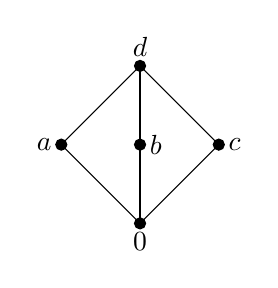
\begin{tikzpicture}
				\filldraw[black] (1,1) circle (2pt) node[above]{$d$};
				\filldraw[black] (0,0) circle (2pt) node[left]{$a$};
				\filldraw[black] (2,0) circle (2pt) node[right]{$c$};
				\filldraw[black] (1,0) circle (2pt) node[right]{$b$};
				\filldraw[black] (1,-1) circle (2pt) node[below]{$0$};
				\draw[-,thin] (1,1)--(0,0)--(1,-1)--(2,0)--(1,1);
				\draw[-,thin] (1,-1)--(1,0)--(1,1);
			\end{tikzpicture}
			\captionof{figure}{}\label{fig:reticolo1}
		\end{minipage}
		\hfil
		\begin{minipage}{.4\textwidth}
			\centering
			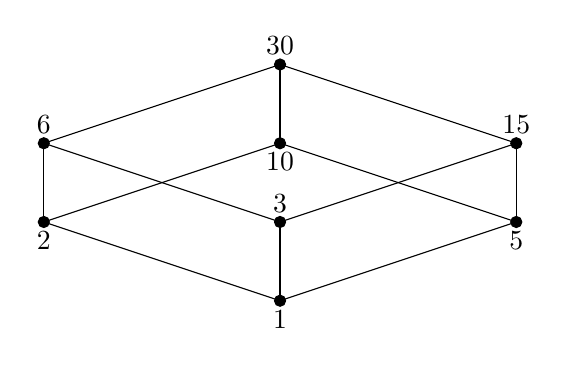
\begin{tikzpicture}
				\filldraw[black] (4,2) circle (2pt) node[below]{$10$};
				\filldraw[black] (4,3) circle (2pt) node[above]{$30$};
				\filldraw[black] (1,2) circle (2pt) node[above]{$6$};
				\filldraw[black] (4,1) circle (2pt) node[above]{$3$};
				\filldraw[black] (7,2) circle (2pt) node[above]{$15$};
				\filldraw[black] (1,1) circle (2pt) node[below]{$2$};
				\filldraw[black] (4,0) circle (2pt) node[below]{$1$};
				\filldraw[black] (7,1) circle (2pt) node[below]{$5$};
				\draw[-,thin] (4,2)--(7,1);
				\draw[-,thin] (7,2)--(7,1);
				\draw[-,thin] (7,1)--(4,0);
				\draw[-,thin] (1,1)--(1,2);
				\draw[-,thin] (1,2)--(4,3);
				\draw[-,thin] (1,2)--(4,1);
				\draw[-,thin] (4,1)--(7,2);
				\draw[-,thin] (4,2)--(1,1);
				\draw[-,thin] (4,2)--(4,3);
				\draw[-,thin] (4,3)--(7,2);
				\draw[-,thin] (1,1)--(4,0);
				\draw[-,thin] (4,1)--(4,0);
			\end{tikzpicture}
			\captionof{figure}{}\label{fig:reticolo2}
		\end{minipage}
		\hfil
		\begin{minipage}{.3\textwidth}
			\centering
			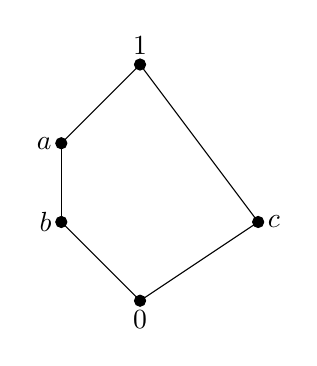
\begin{tikzpicture}
				\filldraw[black] (3,3) circle (2pt) node[above]{$1$};
				\filldraw[black] (2,2) circle (2pt) node[left]{$a$};
				\filldraw[black] (2,1) circle (2pt) node[left]{$b$};
				\filldraw[black] (3,0) circle (2pt) node[below]{$0$};
				\filldraw[black] (4.5,1) circle (2pt) node[right]{$c$};
				\draw[-,thin] (3,3)--(2,2);
				\draw[-,thin] (2,2)--(2,1);
				\draw[-,thin] (2,1)--(3,0);
				\draw[-,thin] (3,0)--(4.5,1);
				\draw[-,thin] (4.5,1)--(3,3);
			\end{tikzpicture}
			\captionof{figure}{}\label{fig:reticolo3}
		\end{minipage}
	\end{center}
	sono complementati. Nel caso del reticolo mostrato in Figura \ref{fig:reticolo1} l'elemento $a$ ha due complementi ($b$ e $c$) così come $b$ e $c$ hanno due complementi ciascuno. Analogamente, nel reticolo \ref{fig:reticolo3} l'elemento $c$ ha più di un complemento: $a$ e $b$ sono entrambi complementi di $c$ mentre $a$ e $b$ hanno entrambi un unico complemento ($c$). Nel caso del reticolo \ref{fig:reticolo2} ogni elemento ha un unico complemento. Notiamo inoltre che tale reticolo corrisponde all'insieme $Div(30)$ e che il complemento di ogni $k \in Div(30)$ corrisponde all'elemento $\frac{30}{k}$.
\end{example}

\begin{defbox}{Reticolo distributivo}
	Sia $(S,\wedge,\vee)$ un reticolo. Allora $(S,\leq)$ è \textbf{distributivo} se e soltanto se, per ogni $a,b,c \in S$:
	\begin{displaymath}
		\begin{array}{l}
			a \vee (b \wedge c) = (a \vee b) \wedge (a \vee c)\\
			a \wedge (b \vee c) = (a \wedge b) \vee (a \wedge c)
		\end{array}
	\end{displaymath}
	ossia $\wedge$ è distributiva rispetto a $\vee$ e viceversa.
\end{defbox}

\begin{example}
	Il reticolo delle parti di un insieme $S$ è distributivo in quanto $\cap$ e $\cup$ sono distributive l'una rispetto all'altra.
\end{example}


\begin{propbox}
	Se $(S,\leq)$ è un reticolo limitato distributivo, allora ogni $a \in S$ ammette unico complemento.
\end{propbox}


\begin{proof}
	Supponiamo per assurdo che $x$ e $y$ siano entrambi complementi di $a$ e sia $0= min S$ e $1= max S$. Allora:
	\begin{displaymath}
		\begin{array}{l}
			a \wedge x = 0 = a \wedge y \\
			a \vee x = 1 = a \vee y
		\end{array}
	\end{displaymath}
	Allora:
	\begin{displaymath}
		x = x \wedge 1 = x \wedge (a \vee y) = (x \wedge a) \vee (x \wedge y) = 0 \vee (x \wedge y) = x \wedge y
	\end{displaymath}
	Analogamente $y= y \wedge x$. Per la proprietà commutativa delle operazioni reticolari allora si ha $x=y$. 
\end{proof}

\begin{example}
	La distributività del reticolo è una condizione necessaria per l'unicità del complemento. Si consideri il seguente reticolo:
	\begin{center}
		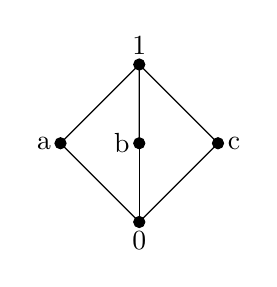
\begin{tikzpicture}
			\filldraw[black] (1,1) circle (2pt) node[anchor=south]{1};
			\filldraw[black] (0,0) circle (2pt) node[anchor=east]{a};
			\filldraw[black] (2,0) circle (2pt) node[anchor=west]{c};
			\filldraw[black] (1,-1) circle (2pt) node[anchor=north]{0};
			\filldraw[black] (1,0) circle (2pt) node[anchor=east]{b};
			\draw[-,thin] (1,0)--(1,1)--(0,0)--(1,-1)--(2,0)--(1,1);
			\draw[-,thin](1,0)--(1,-1);
		\end{tikzpicture}
	\end{center}
	Si ha chiaramente $\forall x(0 \leq x)$  e $\forall x (x \leq 1)$ ed inoltre i punti $a,b,c$ non sono confrontabili tra di loro. Allora chiaramente sia $b$ che $c$ sono dei complementi per $a$ ed infatti il reticolo non è distributivo:
	\begin{displaymath}
		a \vee (b \wedge c) = a \vee 0 = a
	\end{displaymath}
	mentre:
	\begin{displaymath}
		(a \vee b) \wedge (a \vee c) = 1 \wedge 1 = 1
	\end{displaymath}
	
	Inoltre, non è detto che se ogni elemento ha un unico complemento nel reticolo allora questo risulti distributivo. Non vale ovvero l'implicazione inversa.
	
\end{example}

\begin{defbox}{Reticolo pentagonale}
	Si consideri un insieme $X= \{x_{1},x_{2},x_{3},x_{4},x_{5}\}$ di ordine 5 e si introduca in $X$ una relazione d'ordine ponendo $\forall x \in X \bigl(x \leq x, \ x_{1} \leq x, \ x \leq x_{5} \bigr)$ e inoltre $x_{2} \leq x_{3}$. Allora $\{x_{2},x_{4}\}$ e $\{x_{3},x_{4}\}$ sono gli unici sottoinsiemi di ordine $2$ di $X$ costituiti da elementi non confrontabili, e si ha $x_{1}= inf\{x_{2},x_{4}\}=inf\{x_{3},x_{4}\}$ e $x_{5}=sup\{x_{3},x_{4}\}$ Il reticolo $(X,\wedge,\vee)$ associato all'insieme ordinato $(X,\leq)$ si chiama \textbf{reticolo pentagonale}.
\end{defbox}


\begin{defbox}{Reticolo trirettangolo}
	Sia $Y=\{y_{1},y_{2},y_{3},y_{4},y_{5}\}$ un altro insieme di ordine 5 e si introduca in $Y$ una relazione d'ordine $\leq$ ponendo $y \leq y$, $y_{1} \leq y$ e $y \leq y_{5}$ per ogni $y \in Y$. Allora $\{y_{2},y_{3}\}$, $\{y_{2},y_{4}\}$ e $\{y_{3},y_{4}\}$ sono i sottoinsiemi di ordine 2 di $Y$ costituiti da elementi non confrontabili, e si ha $y_{1}=inf\{y_{2},y_{3}\}=inf\{y_{2},y_{4}\}=inf\{y_{3},y_{4}\}$. Il reticolo $(Y,\wedge,\vee)$ associato all'insieme ordinato $(Y,\leq)$ si chiama \textbf{reticolo trirettangolo}.
\end{defbox}

	\begin{center}
\begin{minipage}{.45\textwidth}
	\centering
		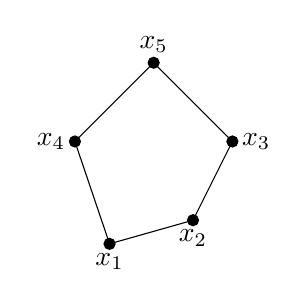
\begin{tikzpicture}
		\filldraw[black] (2,3) circle (2pt)node[anchor=south]{$x_{5}$};
		\filldraw[black] (3,2) circle (2pt)node[anchor=west]{$x_{3}$};
		\filldraw[black] (1,2) circle (2pt)node[anchor=east]{$x_{4}$};
		\filldraw[black] (1.44,0.7) circle (2pt) node[anchor=north]{$x_{1}$};
		\filldraw[black] (2.5,1) circle (2pt)node[anchor=north]{$x_{2}$};
		\draw[-,thin] (2,3)--(1,2)--(1.44,0.7)--(2.5,1)--(3,2)--(2,3);
	\end{tikzpicture}
\captionof{figure}{Reticolo pentagonale}
\end{minipage}
\hfil
\begin{minipage}{.45\textwidth}
	\centering
			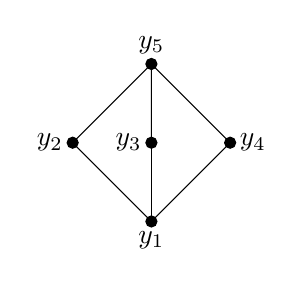
\begin{tikzpicture}
			\filldraw[black] (1,1) circle (2pt) node[anchor=south]{$y_{5}$};
			\filldraw[black] (0,0) circle (2pt) node[anchor=east]{$y_{2}$};
			\filldraw[black] (2,0) circle (2pt) node[anchor=west]{$y_{4}$};
			\filldraw[black] (1,-1) circle (2pt) node[anchor=north]{$y_{1}$};
			\filldraw[black] (1,0) circle (2pt) node[anchor=east]{$y_{3}$};
			\draw[-,thin] (1,0)--(1,1)--(0,0)--(1,-1)--(2,0)--(1,1);
			\draw[-,thin](1,0)--(1,-1);
		\end{tikzpicture}
	\captionof{figure}{Reticolo trirettangolo}
\end{minipage}
	\end{center}


Per capire se un reticolo è distributivo, ne costruisco il diagramma di Hasse e verifico se questo contiene un sottoreticolo pentagonale o trirettangolo. Se un reticolo li contiene, eredita a sua volta le proprietà dei sottoreticoli. Infatti, un reticolo isomorfo ad un altro reticolo ha le sue stesse proprietà. Vale quindi il seguente teorema.

\begin{teorbox}[Criterio di Birkhoff]\label{thm:birkhoff}
	Sia $(S,\leq)$ un reticolo, allora $(S,\leq)$ è distributivo se e soltanto se nessun sottoreticolo di $(S,\leq)$ è isomorfo ad un reticolo pentagonale o trirettangolo.
\end{teorbox}

\begin{corolbox}
	I reticoli pentagonali e trirettangolo sono i più piccoli tra i reticoli non distributivi. Ogni reticolo di ordine inferiore a 5 è distributivo.
\end{corolbox}

\pagebreak
\section{Strutture booleane}
\subsection{Anelli booleani}
\begin{defbox}{Anello booleano}
	Un anello $A$ si dice \textbf{booleano} se $A$ è unitario ed ogni elemento è idempotente, cioè coincide col proprio quadrato: $\forall a \in A \bigl(a = a \cdot a\bigr)$.
\end{defbox}

\begin{example}
	L'anello $(\mathcal{P}(S),\triangle,\cap)$ delle parti di un insieme è un anello booleano. Infatti è unitario e dal momento che l'operazione di moltiplicazione dell'anello $\mathcal{P}(S)$ è quella di intersezione, per ogni $X \in \mathcal{P}(S)$ si ha $X^{2}= X \cap X = X$.
\end{example}

\begin{defbox}{Caratteristica di un anello}
	Se $A$ è unitario e indichiamo l'unità di $A$ con $1_{A}$, se esiste qualche intero positivo $n \in \mathbb{Z^{+}}$ tale che:
	\begin{displaymath}
		n 1_{A} = 1_{A}+ 1_{A}+ \dots + 1_{A} = 0_{A}
	\end{displaymath}
	allora la \textbf{caratteristica} di $A$ è il minimo tale intero $n$.
\end{defbox}


\begin{osservation}
	Ovviamente $A$ ha caratteristica 1 se e soltanto se $1_{A}=0_{A}$ e quindi $A=\{0_{A}\}$. Altrettanto banale è il caso in cui la caratteristica di $A$ è due, per cui $1_{A} \neq 0_{A}$ e risulta $2 \cdot 1_{A}=0_{A}$. Notiamo che l'anello $(\mathcal{P}(S),\triangle, \cap)$ ha questa proprietà se $S \neq \emptyset$. Infatti in questo anello l'unità è $S$, lo zero è $\emptyset$, l'addizione è la differenza simmetrica e si ha $ 2 \cdot S = S \triangle S = \emptyset$. Quindi l'anello $\mathcal{P}(S)$ ha caratteristica 2.
\end{osservation}
Dimostriamo  ora che quanto appena visto per $(\mathcal{P}(S),\triangle, \cap)$ vale per tutti gli anelli booleani; verificando inoltre che questi anelli sono sempre commutativi.

\begin{propbox}
	Sia $A$ un anello booleano, allora $A$ è commutativo e, se $|A|>1$ allora $A$ ha caratteristica 2.
\end{propbox}

\begin{proof}
	Per ogni $a,b \in A$ vale: $a^{2}=a \cdot a = a$, $b^{2}= b \cdot b = b$. Quindi:
	\begin{align*}
		(a+b)^{2}&=(a+b)(a+b)\\
		&= a(a+b) + b(a+b)\\
		&= a^{2} + ab + ba + b^{2}\\
		&= a + ab + ba + b
	\end{align*}
	Essendo la caratteristica di $A$ pari a due, però, si ha che $(a+b)^{2}=(a+b)$ quindi:
	\begin{align*}
		a + ab + ba + b &= a+b \\
		&\implies ab+ba = 0_{A} \\
		&\implies ab = -ba
	\end{align*}
	Nel caso in cui sia $a=b$ si ottiene che, per ogni $a \in A$ vale $a^{2}=-a^{2}$ ovvero $a=-a$. Quindi $\forall a \in A$ si ha $2a = 0_{A}$. In particolare $2 \cdot 1_{A} = 0_{A}$, quindi o $1_{A}=0_{A}$ ed $A=\{0_{A}\}$ oppure $|A|>1$ e la caratteristica di $A$ è due. Infine, per ogni $a,b$, sfruttando $a=-a$ per l'elemento $ba$ si ha: $ba = -ba = ab$ ed $A$ risulta commutativo. 
\end{proof}

Enunciamo ma non dimostriamo il teorema di Stone, che è il risultato fondamentale nella teoria degli anelli booleani.

\begin{teorbox}[di Stone]
	Sia $A$ un anello booleano, allora:
	\begin{itemize}
		\item Esiste un insieme $S$ tale che $A$ sia isomorfo ad un sottoanello unitario di $(\mathcal{P}(S),\triangle,\cap)$;
		\item Se $A$ è finito esiste un insieme $S$ tale che $A$ sia isomorfo a $(\mathcal{P}(S),\triangle,\cap)$.
	\end{itemize}
\end{teorbox}

\begin{osservation}
	Tutti i sottoanelli unitari di $(\mathcal{P}(S),\triangle,\cap)$ sono booleani.
\end{osservation}


\begin{corolbox}
	Sia $R$ un anello booleano finito. Allora:
	\begin{enumerate}
		\item Esiste $n\in \mathbb{N}$ tale che $|R|=2^{n}$;
		\item Se $A$ è un anello booleano e $|A| = |R|$ allora $A \simeq R$.
	\end{enumerate}
\end{corolbox}

\begin{proof}
	Per il teorema di Stone, esiste un insieme $S$, ovviamente finito, tale che $R$ sia isomorfo a $(\mathcal{P}(S),\triangle,\cap)$. Posto $n=|S|$, allora $|R| = |\mathcal{P}(S)| = 2^{n}$, il che giustifica la (1). Se poi $A$ è un anello booleano, anch'esso di cardinalità $2^{n}$, ancora per il teorema di Stone abbiamo $A \simeq (\mathcal{P}(T),\triangle,\cap)$ per un opportuno insieme $T$. Ma allora $|\mathcal{P}(T)| = |A|$, quindi $|\mathcal{P}(T)|=2^{n}$ e deduciamo così $|T|=n$. Dunque $|T|=|S|$ e quindi $A \simeq R$.
\end{proof}

\subsection{Reticoli booleani}
Ricordiamo che un reticolo è un insieme ordinato non vuoto $(L,\leq)$ tale che, per ogni $a,b \in L$ esistano l'estremo inferiore $inf_{(L,\leq)}\{a,b\}$ e l'estremo superiore $sup_{(L,\leq)}\{a,b\}$ di $\{a,b\}$ in $(L,\leq)$. Ricordiamo anche che si può, in modo equivalente, riguardare i reticoli anche come strutture algebriche.

\begin{defbox}{Reticolo booleano}
	Un reticolo si dice \textbf{booleano} se e solo se è distributivo e complementato.
\end{defbox}

Come abbiamo appena visto, un reticolo può essere visto anche come una struttura algebrica $(L,\wedge,\vee)$. Affinché $L$ sia un reticolo booleano devono valere:
\begin{itemize}
	\item le proprietà commutative per $\wedge$ e $\vee$;
	\item le proprietà associative per $\wedge$ e $\vee$;
	\item le leggi di assorbimento;
	\item le proprietà distributive;
	\item l'esistenza degli elementi neutri di $\wedge$ e $\vee$ (ovvero devono esistere $min$ e $max$ del reticolo);
	\item ogni elemento deve avere un complemento. Esiste quindi l'applicazione\footnote{Che risulta ben posta in quanto il reticolo è distributivo e ogni elemento ammette un unico complemento.}: $': a \in L \mapsto a' \in L$.
\end{itemize}
Gli insiemi totalmente ordinati con massimo due elementi sono reticoli booleani.
\subsection{Algebre di Boole}
\begin{defbox}{Algebra di Boole}
	Si definisce \textbf{algebra di Boole} una struttura algebrica $(L,\vee,\wedge,0,1,')$ tale che:
	\begin{enumerate}
		\item $(L,\vee,0)$ e $(L,\wedge,1)$ sono monoidi commutativi;
		\item valgono le leggi di assorbimento: $\forall a,b \in L \bigl(a \vee(a \wedge b)=a=a\wedge(a \vee b)\bigr)$;
		\item vale la distributività di $\wedge$ rispetto a $\vee$ e viceversa;
		\item per ogni $a \in L$ esiste il complementare $a'$ per il quale $a \wedge a' = 0$ e $a \vee a'=1$.
	\end{enumerate}
	
\end{defbox}

\begin{osservation}
	Ogni reticolo booleano è un'algebra di Boole e viceversa. Infatti, la (1) e la (2) esprimono il fatto che $(L,\wedge,\vee)$ è un reticolo limitato, con minimo $0$ e massimo $1$ mentre la $(3)$ dice che questo reticolo è distributivo e la $(4)$ garantisce che ogni elemento $a$ di $L$ ha un complemento $a'$. Possiamo dunque dire che la nozione di algebra di Boole è la versione ``puramente algebrica'' della nozione di reticolo booleano.
\end{osservation}

\begin{defbox}{Sottoalgebra di Boole}
	Sia $(L,\vee,\wedge,0,1,')$ un'algebra di Boole. Un sottoinsieme $C \subset L$ è detto \textbf{sottoalgebra di Boole} se, per ogni $x,y \in C$:
	\begin{enumerate}
		\item $x \vee y \in C$ e $x \wedge y \in C$
		\item $0 \in C$ e $1 \in C$
		\item $x' \in C$
	\end{enumerate}
\end{defbox}

La nozione di sottoalgebra di Boole differisce da quella di sottoreticolo. Infatti, un sottoreticolo $K$ di un reticolo booleano $L$ deve essere chiuso rispetto alle due operazioni reticolari (quindi deve verificare la prima delle tre condizioni appena elencate), ma non contiene necessariamente il massimo o il minimo del reticolo né, tanto meno, i complementi dei suoi elementi.


\begin{example}
	\begin{enumerate}
		\item Sia $S \neq \emptyset$ un insieme. Consideriamo il reticolo booleano $(\mathcal{P}(S),\subseteq)$. Questo si struttura come algebra di Boole nella forma $(\mathcal{P}(S), \cup, \cap, \emptyset, S, \mathcal{C}_{X})$ dove $\mathcal{C}_{X}$ è l'applicazione ``complemento'' che manda ogni $X \in \mathcal{P}(S)$ in $S \setminus X$.
	
		\item Sia $\mathbb{B}=\{0,1\}$ dotato delle operazioni binarie $\wedge$ e $\vee$ e dell'operazione unaria $'$ dove:
		\begin{enumerate}
			\item $\vee$ (OR) è definita da $0\vee0 = 0$, $0 \vee 1=1 \vee 0 = 1 \vee 1 = 1$ ;
			\item $\wedge$ (AND) è definita da $0 \wedge 0 = 0 \wedge 1 = 1 \wedge 0 = $ e $1 \wedge 1 = 1$;
			\item $0'=1$ e $1'=0$.
		\end{enumerate}
		Si ha che $(\mathbb{B},\vee,\wedge,0,1,')$ è un'algebra di Boole.
	\end{enumerate}
\end{example}

Il prossimo enunciato elenca alcune identità che valgono nelle algebre di Boole. La terza si esprime dicendo che l’operazione di complemento è \textbf{involutoria}, cioè coincide con l’applicazione inversa di sé stessa (e, in particolare, è biettiva); le ultime due sono le note come leggi di De Morgan per algebre di Boole.

\begin{propbox}	
	Sia $(L,\vee,\wedge,0,1,')$ un'algebra di Boole. Allora $\forall a,b \in L$ valgono:
	\begin{enumerate}
		\item $1 \vee a = 1$ e $0 \wedge a = 0 $
		\item $1'=0 $ e $0' = 1$
		\item $(a')'=a $
		\item $(a \vee b)' = a' \wedge b' $
		\item $(a \wedge b)' = a' \vee b'$
	\end{enumerate}
\end{propbox}

\begin{proof}	
	La (1) e la (2) sono immediate in quanto $L$ è un reticolo.
	
	Per dimostrare la validità della (3) basta osservare che $a'$ è un complemento di $a$ e $a$ è un complemento di $a'$, anche $(a')'$ è un complemento di $a'$; quindi per l'unicità dei complementi nei reticoli booleani si ha $a=(a')'$.
	
	Per la $(4)$ basta mostrare che $(a' \wedge b')$ è un complemento di $a \vee b$, ovvero che:
	\begin{displaymath}
		(a \vee b) \vee (a' \wedge b') = 1
	\end{displaymath}
	e:
	\begin{displaymath}
		(a \vee b) \wedge (a' \wedge b') = 0
	\end{displaymath}
	Usando la distributività e la (1) si ottiene:
	\begin{align*}
		(a \vee b) \vee (a' \wedge b') &= (a \vee b \vee a') \wedge (a \vee b \vee b') \\
		&= (1 \vee b) \wedge (a \vee 1) \\
		&= 1 \wedge 1 = 1
	\end{align*}
	e
	\begin{align*}
		(a \vee b) \wedge (a' \wedge b') &= (a \wedge a' \wedge b') \vee (b \wedge a' \wedge b') = (0 \wedge b') \vee (0 \wedge a') \\
		&= 0 \vee 0 = 0
	\end{align*}
	La numero $(5)$ si dimostra in maniera duale.
\end{proof}

\subsection{Anelli booleani e algebre di Boole}

Si rimanda \href{https://www.dma.unina.it/cutolo/didattica/note/strutturebooleane.pdf}{qui} alle note del docente. Argomento cardine di questa sezione è la sostanziale \textit{equivalenza tra concetto di algebra di Boole, reticolo booleano e anello booleano} in quanto esiste una corrispondenza biunivoca fra le tre strutture, nel senso che si può costruire una struttura di reticolo booleano su ogni anello booleano e, viceversa, una struttura di anello booleano su ogni reticolo booleano, in modo che queste due
costruzioni siano l’una inversa dell’altra. Grazie al Teorema di Stone, infatti, ogni anello booleano finito è isomorfo a $(\mathcal{P}(S), \triangle, \cap)$ per un opportuno insieme $S$ (per gli anelli infiniti il teorema è un po' più debole: ogni anello booleano è isomorfo ad un sottoanello unitario di $(\mathcal{P}(S), \triangle, \cap)$, per un opportuno insieme $S$). Analoghi enunciati valgono per i reticoli booleani e per le algebre di Boole. 

In primo luogo, partendo da un anello booleano $(R,+,\cdot)$ vogliamo definire una struttura di reticolo booleano su $R$. L'esempio dell'anello delle parti di un insieme può suggerirci in che modo procedere. Fissato un insieme $S$, infatti, $(\mathcal{P}(S), \triangle, \cap)$ è un anello booleano ma $\mathcal{P}(S)$ è anche un reticolo booleano, con operazioni reticolari $\cup$ e $\cap$. La seconda operazione reticolare è proprio l'operazione di moltiplicazione nell'anello. Anche la prima operazione reticolare si può esprimere in termini delle operazioni dell'anello: per ogni $A,B \in \mathcal{P}(S)$ abbiamo infatti che:
\begin{displaymath}
	A \cup B = (A \triangle B) \cup (A \cap B) = (A \triangle B) \triangle (A \cap B)
\end{displaymath}
Inoltre, il minimo ed il massimo del reticolo sono $\emptyset$ e $S$, cioè lo zero e l'unità dell'anello, e ciascun $A \in \mathcal{P}(S)$ ha come complemento, nel reticolo $(\mathcal{P}(S),\subseteq)$ l'insieme $S \setminus A = S \triangle A = 1_{\mathcal{P}(S)} \triangle A$.

Passando ora ad un arbitrario anello booleano $(R,+,\cdot,0_{R},1_{R})$ dove $0_{R}$ e $1_{R}$ sono lo zero e l'unità dell'anello, l'esempio di $\mathcal{P}(S)$ suggerisce di definire in $R$ l'operazione binaria $\vee$ ponendo, per ogni $a,b \in R$:
\begin{equation}
	a \vee b \coloneqq a+b+ab
\end{equation}
e l'applicazione $':a \in R \mapsto 1_{R}+a \in R$ da utilizzare come operazione unaria di complemento.


\begin{propbox}
	Con le notazioni appena fissate, $(R,\vee, \cdot, 0_{R},1_{R},')$ è un'algebra di Boole.
\end{propbox}

\begin{proof}
	Dobbiamo verificare che $(R, \vee, 0_{R})$ e $(R, \cdot, 1_{R})$ siano monoidi commutativi, che valgano per $\vee$ e $\cdot$ le leggi di assorbimento e le proprietà distributive ed infine che l’applicazione $'$ verifichi la condizione richiesta dalla definizione di complemento.
	
	Che $\vee$ sia commutativa è evidente, ed è anche chiaro che $a \vee 0_{R} = a + 0_{R}+ a0_{R}$ per ogni $a \in R$, quindi $0_{R}$ è neutro rispetto a $\vee$. Proviamo l'associatività di $\vee$: per ogni $a,b,c \in R$ si ha:
	\begin{align*}
		(a \vee b) \vee c &= (a+b+ab) \vee c \\
		&= (a+b+ab) + c + (a+b+ab)c \\
		&= a+b+ab+c+ac+bc+abc
	\end{align*}
	Si ha inoltre:
	\begin{align*}
		a \vee (b \vee c) &= (b \vee c) \vee a \\
		&= b+c+a+bc+ba+ca+bca
	\end{align*}
	dunque $(a \vee b) \vee c = a \vee (b \vee c)$. È così provato che $\vee$ è associativa. $(R,\vee,0_{R})$ è un monoide commutativo. Che lo sia anche $(R,\cdot,1_{R})$ è già noto in partenza, dal momento che $R$ è un anello booleano.
	
	Verifichiamo le leggi di assorbimento. Per ogni $a,b \in R \bigl(a \vee (ab) = a +ab+a(ab) \bigr)$. Dal momento che $R$ è booleano, $a(ab) = a^{2}b = ab$ e $ab+ab=0_{R}$, quindi $a \vee  (ab) = a+ab+ab = a$. Inoltre $a(a \vee b) = a(a+b+ab) = a^{2}+ab+a^{2}b = a+ab+ab=a$. Le leggi di assorbimento sono così provate. A questo punto possiamo concludere che $(R,\vee,\cdot)$ è un reticolo limitato.
	
	Verifichiamo ora che $\cdot$ è distributiva rispetto a $\vee$. Per ogni $a,b,c \in R$ si ha $a(b \vee c) = a(b+c+bc)=ab+ac+abc$ e $(ab) \vee (ac) = ab+ac+(ab)(ac) = ab+ac+abc$. Dunque $a(b \vee c) = (ab) \vee (ac)$. Pertanto, utilizzando anche la proprietà commutativa, possiamo concludere che $\cdot$ è distributiva rispetto a $\vee$.
	
	Resta infine da dimostrare che, per ogni $a \in R$, l'immagine di $a$ mediante l'applicazione $'$, vale a dire $a' \coloneqq 1_{R}+a$, verifica le condizioni $a \vee (1_{R}+a)= 1_{R}$ e $aa' = 0_{R}$. Questo è molto facile: per ogni $a \in R$ si ha $aa'=a(1_{R}+a) = a+a = 0_{R}$ e $a \vee a' = a+a'+aa' = a+(1_{R}+a)+0_{R}=1_{R}$, come richiesto. Con questo la dimostrazione è completa. 
\end{proof}

Descriviamo ora la costruzione inversa: quella di un anello booleano a partire da un’algebra di Boole. Anche in questo caso ci facciamo guidare dall'esempio dell'algebra $(\mathcal{P}(S), \cup, \cap, \emptyset, S, \mathcal{C}_{X})$ delle parti di un insieme $S$. Delle due operazioni binarie dell'anello booleano $(\mathcal{P}(S),\triangle,\cap)$, quella di moltiplicazione, $\cap$, è già tra le operazioni dell'algebra di Boole. Per esprimere l'altra, la differenza simmetrica, utilizzando le operazioni dell'algebra di Boole ci è utile osservare che se $A$ e $B$ sono parti di $S$, allora $A \setminus B = A \cap (S \setminus B) = A \cap \mathcal{C}_{X}(B)$. Dunque $A \triangle B$ può essere scritta come:
\begin{displaymath}
	\begin{cases}
		(A \setminus B) \cup (B \setminus A)  = (A \cap \mathcal{C}_{X}(B)) \cup (B \cap \mathcal{C}_{X}(A)) \\
		(A \cup B ) \setminus (A \cap B) = (A \cup B) \cap (\mathcal{C}_{X}(A \cap B))
	\end{cases}
\end{displaymath}

Questo esempio mostra due modi possibili per definire, in un'arbitraria algebra di Boole, un'operazione binaria di addizione $+$ analoga alla differenza simmetrica in $\mathcal{P}(S)$.


\begin{lemmabox}
	Sia $(L,\vee,\wedge,0,1,')$ un'algebra di Boole. Allora, per ogni $a,b \in L$:
	\begin{displaymath}
		(a \wedge b') \vee (a' \wedge b) = (a \vee b) \wedge (a \wedge b) '
	\end{displaymath}
	
\end{lemmabox}
\begin{proof}
	Usando la proprietà distributiva di $\vee$ rispetto a $\wedge$ abbiamo:
	\begin{align*}
		(a \wedge b') \vee (a' \wedge b) &= (a \vee a') \wedge (a \vee b) \wedge (b' \vee a') \wedge (b' \vee b) \\
		&= 1 \wedge (a \vee b) \wedge (b' \vee a') \wedge 1 \\
		&= (a \vee b) \wedge (a' \vee b') \\
		&= (a \vee b) \wedge (a \wedge b)'
	\end{align*}
	avendo utilizzato, per ultimo passaggio, una delle leggi di De Morgan.
\end{proof}


\begin{teorbox}[di Stone per le algebre di Boole]
	Ogni reticolo booleano finito è isomorfo al reticolo finito delle parti. Ogni algebra di Boole è isomorfa ad un'algebra di Boole delle parti finite.
\end{teorbox}

Questo vuol dire, ad esempio, che se sappiamo descrivere il reticolo delle parti degli insiemi finiti, conosciamo, a meno di isomorfismi, tutti i reticoli booleani finiti. Una conseguenza del teorema di Stone è che gli anelli booleani finiti (ma lo stesso vale per i reticoli booleani finiti o per le algebre di Boole finite) hanno per cardinalità una potenza di 2, e che due anelli booleani finiti con lo stesso numero di elementi sono necessariamente isomorfi.

Sia allora $X \subseteq S$. Prendiamo la funzione caratteristica: \begin{displaymath}
\mbox{\Large$\chi$}_{X,S}: x \in S \mapsto \begin{cases*}
		0 & \text{ se} x \notin X \\
		1 & \text{ se} x \in X
	\end{cases*} \in \{0,1\}
\end{displaymath}
e alteriamone il codominio:
\begin{displaymath}
	\mbox{\Large$\chi$}_{X,S}: x \in S \mapsto \begin{cases*}
		\overline{0} & \text{ se} x \notin X \\
		\overline{1} & \text{ se} x \in X
	\end{cases*}
\in \mathbb{Z}_{2}
\end{displaymath}
Dimostriamo che $X \in \mathcal{P}(S) \mapsto \mbox{\Large$\chi$}_{X,S} \in Map(S,\mathbb{Z}_{2})$ è biettiva. Sia $S=\{1,2,3,\ldots,n\}$ con $n \in \mathbb{N}^{*}$. Allora $Map(S,\mathbb{Z}_{2})$ è l'insieme delle $n$-ple di elementi di $\mathbb{Z}_{2}$. Come già osservato, possiamo scrivere ogni funzione da $S$ in $\mathbb{Z}_{2}$ come una stringa $(s_{1}s_{2}\ldots s_{n})$. Chiamiamo $\mathbb{Z}_{2}^{n}$ l'insieme di tali stringhe, gli elementi di $\mathcal{P}(S)$ corrispondono quindi a tali stringhe.

Sia allora $R^{n} = R \times \cdots \times R$ il prodotto cartesiamo di $n$ copie di un anello $R$, ovvero l'insieme di $n$-ple di elementi di $R$. Se prendiamo due elementi e ne facciamo somma e prodotto, otteniamo:
\begin{align*}
	a+b = (a_{1}+b_{1}, a_{2}+b_{2}, \ldots, a_{n}+b_{n})\\
	a \cdot b = (a_{1}\cdot b_{1}, a_{2}\cdot b_{2}, \ldots, a_{n}\cdot b_{n})
\end{align*}
E possiamo considerare la struttura $(R^{n},+,\cdot)$ che risulta essere un anello. Se $R$ è booleano, anche $R^{n}$ è booleano. Allora anche $\mathbb{Z}_{2}^{n}$, per le stesse osservazioni, sarà un anello booleano rispetto alle operazioni di somma e prodotto.

\begin{example}
	Sia $S=\{1,2,3,4,5,6,7,8\}$ e consideriamo le stringhe $a=(10010011)$ e $b=(01101101)$, facendo somma e prodotto, otteniamo:
	\begin{align*}
		a+b = 1111 1110 = a \xor b\\
		a \cdot b = 0000 0001 = a \wedge b
	\end{align*}
dove $\xor$ e $\wedge$ sono i classici operatori logici bit a bit. Sappiamo inoltre che l'applicazione $X \in \mathcal{P}(S) \mapsto \mbox{\Large$\chi$}_{X,S} \in \mathbb{Z}_{2}^{8}$ è biettiva. Quindi prese le parti $A=\{1,4,7,8\}$ e $B=\{2,3,5,6,8\}$, codificate dalle stringhe $a=(10010011)$ e $b=(01101101)$, abbiamo:
\begin{align*}
	a+b =(11111110) = \{1,2,3,4,5,6,7\} = A \triangle B\\
	a \cdot b = 00000001 = \{8\} = A \cap B
\end{align*}
Allora $X\in \mathcal{P}(S) \mapsto \mbox{\Large$\chi$}_{X,S} \in \mathbb{Z}_{2}^{n}$ è un isomorfismo di anelli.
\end{example}

Nel caso finito, come anticipato, tutte le algebre di Boole sono isomorfe a $\mathcal{P}(S)$.

\begin{osservation}
	I simboli che si usano per le operazioni reticolari coincidono con i simboli usati per i connettivi logici perché è possibile definire una struttura con l'insieme di tutte le formule con i connettivi logici come operazioni, che descrivono relazioni di equivalenza. L'insieme quoziente che ne deriva è proprio un'algebra di Boole. Per questo motivo si usano gli stessi simboli e per questo motivo le algebre di Boole rivestono un ruolo importante in logica ed in informatica.
\end{osservation}
\newpage
\section{Esercizi svolti}
\subsection{Relazioni d'ordine e reticoli}
\begin{exsbox}
	Trovare un isomorfismo di reticoli dall'insieme di parti $\{0,1\}$ all'insieme delle parti $\{3,4\}$, ordinati per inclusione.
\end{exsbox}
\begin{exsbox}
	Stabilire per quali interi $n$ nell'insieme $\{2,14,18,27,30\}$ il reticolo dei numeri naturali divisori di $n$ (sottoreticolo di $(\mathbb{N},\divides)$) è complementato.
\end{exsbox}
\begin{exsbox}
	2 ha un complemento in $(\mathbb{N},\divides)$? Il reticolo $(\mathbb{N},\divides)$ è complementato?
\end{exsbox}
\begin{exsbox}
	Disegnare il diagramma di Hasse di un reticolo in cui esista un elemento con sei complementi.
\end{exsbox}
\begin{exsbox}
	Trovare, tra i sottoinsiemi di $\mathcal{P}(\mathbb{N})$, ordinati per inclusione:
	\begin{enumerate}
		\item Un sottoinsieme di cardinalità 5 che non sia un reticolo;
		\item Un sottoinsieme di cardinalità 5 che sia un reticolo trirettangolo;
		\item Un sottoinsieme di cardinalità 5 che sia un reticolo pentagonale.
	\end{enumerate}
\end{exsbox}
\paragraph{Svolgimento.} Abbiamo:
\begin{enumerate}[label=(\textit{\roman*})]
	\item Basterà prendere un insieme di 5 singleton. Ovviamente saranno inconfrontabili rispetto all'inclusione e quindi non costituiscono un reticolo.
	\item Consideriamo $A=\{ \emptyset, \{0\},\{1\},\{2\}, \{1,2,3\} \}$. Si ottiene il reticolo trirettangolo:
	\begin{center}
		\begin{tikzpicture}
			\filldraw[black] (1,1) circle (2pt) node[anchor=south]{$\{1,2,3\}$};
			\filldraw[black] (0,0) circle (2pt) node[anchor=east]{$\{1\}$};
			\filldraw[black] (2,0) circle (2pt) node[anchor=west]{$\{2\}$};
			\filldraw[black] (1,-1) circle (2pt) node[anchor=north]{$\emptyset$};
			\filldraw[black] (1,0) circle (2pt) node[anchor=east]{$\{3\}$};
			\draw[-,thin] (1,0)--(1,1)--(0,0)--(1,-1)--(2,0)--(1,1);
			\draw[-,thin](1,0)--(1,-1);
		\end{tikzpicture}
	\end{center}
	\item Consideriamo $B=\{\emptyset, \{1\}, \{2\}, \{2,3\},\{1,2,3\} \}$. Si ottiene il reticolo pentagonale:
	\begin{center}
		\begin{tikzpicture}
			\filldraw[black] (2,3) circle (2pt)node[anchor=south]{$\{1,2,3\}$};
			\filldraw[black] (3,2) circle (2pt)node[anchor=west]{$\{2,3\}$};
			\filldraw[black] (1,1) circle (2pt)node[anchor=east]{$\{1\}$};
			\filldraw[black] (2,0) circle (2pt) node[anchor=north]{$\emptyset$};
			\filldraw[black] (3,1) circle (2pt)node[anchor=north]{$\{2\}$};
			\draw[-,thin] (2,3)--(1,1)--(2,0)--(3,1)--(3,2)--(2,3);
		\end{tikzpicture}
	\end{center}
\end{enumerate}
\begin{exsbox}
	Dimostrare in modo diretto che gli insiemi totalmente ordinati sono reticoli distributivi.
\end{exsbox}
\paragraph{Svolgimento.} Sia $(S,\leq)$ un insieme totalmente ordinato. Ovviamente, per definizione di relazione d'ordine totale, per ogni parte $\{a,b\}$ di elementi di $S$ esiste un minimo ed un massimo, in quanto vale $a \leq b$ oppure $b \leq a$. Ovvero, posto $a \leq b$:
\begin{align*}
	a \wedge b = inf(\{a,b\}) = a \\
	a \vee b =  sup(\{a,b\}) = b
\end{align*}Si determina cioè una catena. Presi quindi $a,b,c \in S(a \leq b \leq c)$, vale:
\begin{align*}
	a \vee (b \wedge c) =  a \vee b = b \\
	(a \vee b) \wedge (a \vee c) = b \wedge c = b
\end{align*}
E vale:
\begin{align*}
	a \wedge(b \vee c) = a \wedge c  = a\\
	(a \wedge b) \vee (a \wedge c) = a \vee a = a 
\end{align*}
Quindi il reticolo risulta essere distributivo. \hfill \blacksquare
\begin{exsbox}
	Sia $X=\{n \in \mathbb{N} \; | \; 1 \leq n \leq 10\}$. Si considerino i seguenti insiemi di parti di $X$:
	\begin{align*}
		A = \bigl\{\{1,3,5\},\{4,6\}, \{1,7,8\},\{9,10\}\bigr\} \\
		B= \bigl\{\{4\}, \{5,8\},\{1,2,3\},\{6,7,9,10\}\bigr\}
	\end{align*}
Quale tra $A$ e $B$ è una partizione di $X$? Quale non lo è? (giustificare \textit{entrambe} le risposte).
Detta $F$ quella tra $A$ e $B$ che è una partizione di $X$, per ogni $x \in X$ si indichi con $F_{x}$ l'unico elemento di $F$ tale che $x \in F_{x}$. Si consideri in $X$ la relazione binaria $\Sigma$ così definita:
\begin{align*}
	\forall x,y \in X \bigl(x \ \Sigma \ y \iff (x=y \lor |F_{x}| < |F_{y}|)\bigr)
\end{align*}
\begin{enumerate}[label=(\textit{\roman*})]
	\item Si verifichi che $\Sigma$ è una relazione d'ordine in $X$ e si dica se è totale.
	\item Disegnare il diagramma di Hasse di $(X,\Sigma)$
	\item $(X,\Sigma)$ è un reticolo?
	\item Determinare un sottoinsieme di $X$ di ordine 6 tale che $(Y,\Sigma)$ sia un reticolo. $(Y,\Sigma)$ è distributivo? È complementato?
\end{enumerate}
\end{exsbox}
\paragraph{Svolgimento.} Chiaramente $A$ \textit{non} è una partizione di $X$ in quanto risultano essere presenti parti non disgiunte ed elementi di $X$ mancanti. Ad esempio $\{1,3,5\} \cap \{1,7,8\} = \{1\}$ e $\neg(\exists y \in A)(\{2\}\subseteq y)$. L'insieme delle parti $B$ risulta invece essere una partizione per $X$ in quanto ogni elemento di $B$ è disgiunto da qualsiasi altro elemento della partizione e l'unione unaria di $B$ coincide con $X$. Possiamo quindi porre $F=B$.
\begin{enumerate}[label=(\textit{\roman*})]
	\item Dimostriamo che $\Sigma \in OL(X)$:
	\begin{itemize}
		\item Sicuramente $\Sigma$ è riflessiva in quanto per ogni $x \in X$ vale $x \ \Sigma \ x$ dato che $x=x$.
		\item Siano $x,y \in X$ tale che $x \ \Sigma \ y$ e $y \ \Sigma \ x$. Allora o $x=y$, per definizione della relazione $\Sigma$, oppure, da $|F_{x}|< |F_{y}|$ e $|F_{y}|<|F_{y}|$ segue $|F_{x}|=|F_{y}|$. Poiché in $F$ non sono presenti parti equipotenti devono coincidere $F_{x}$ ed $F_{y}$ per avere lo stesso numero di elementi. Quindi $x,y \in F_{x}$. Ma essendo per ipotesi $x \ \Sigma \ y$ e $y \ \Sigma \ x$ e $|F_{x}| \cancel{<} |F_{x}|$ deve essere per forza $x=y$. Quindi $\Sigma$ risulta essere antisimmetrica.
		\item Siano $x,y,z \in X$ tali che $x \ \Sigma \ y$ e $y \ \Sigma \ z$. Allora o è $x=y$ e $y=z$, da cui $x=z$ e quindi $x \ \Sigma \ z$, oppure $|F_{x}| < |F_{y}| < |F_{z}|$ da cui $|F_{x}| < |F_{z}|$ e $x \ \Sigma \ z$. Quindi $\Sigma$ è transitiva e quindi una relazione d'ordine in $X$.
	\end{itemize}
\item Osservando l'insieme $B$ possiamo osservare che $\Sigma$ è determinata dall'ordine stretto tra le cardinalità delle parti di $B$:
\begin{displaymath}
|\{4\}| < |\{5,8\}| <|\{1,2,3\}| < |\{6,7,9,10\}|
\end{displaymath}
Due elementi nello stesso $F_{x}$ sono in relazione $\Sigma$ se e solo se questi coincidono. Quindi due elementi distinti risultano sempre inconfrontabili in uno stesso $F_{x}$. Otteniamo quindi il seguente diagramma di Hasse:
\begin{center}
	\begin{tikzpicture}
		\filldraw[black] (0,0) circle(2pt) node[anchor=north]{4};
		\filldraw[black] (-0.5,1) circle(2pt) node[anchor=north]{5};
		\filldraw[black] (0.5,1) circle(2pt) node[anchor=north]{8};
		\filldraw[black] (-1,2) circle(2pt) node[anchor=north]{1};
		\filldraw[black] (0,2) circle(2pt) node[anchor=north]{2};
		\filldraw[black] (1,2) circle(2pt) node[anchor=north]{3};
		\filldraw[black] (-1.5,3) circle(2pt) node[anchor=south]{6};
		\filldraw[black] (-0.5,3) circle(2pt) node[anchor=south]{7};
		\filldraw[black] (0.5,3) circle(2pt) node[anchor=south]{9};
		\filldraw[black] (1.5,3) circle(2pt) node[anchor=south]{10};
		\draw[black](0,0)--(-0.5,1);
		\draw[black](0,0)--(0.5,1);
		
		\draw[black](0.5,1)--(-1,2);
		\draw[black](0.5,1)--(0,2);
		\draw[black](0.5,1)--(1,2);
		
		\draw[black](-0.5,1)--(-1,2);
		\draw[black](-0.5,1)--(0,2);
		\draw[black](-0.5,1)--(1,2);
		
		\draw[black](-1,2)--(-1.5,3);
		\draw[black](-1,2)--(-0.5,3);
		\draw[black](-1,2)--(0.5,3);
		\draw[black](-1,2)--(1.5,3);
		
		\draw[black](0,2)--(-1.5,3);
		\draw[black](0,2)--(-0.5,3);
		\draw[black](0,2)--(0.5,3);
		\draw[black](0,2)--(1.5,3);
		
		\draw[black](1,2)--(-1.5,3);
		\draw[black](1,2)--(-0.5,3);
		\draw[black](1,2)--(0.5,3);
		\draw[black](1,2)--(1.5,3);
	\end{tikzpicture}
\end{center}
\item Dato che in un reticolo finito devono esiste minimo e massimo, osservando il fatto che risultano esserci 4 elementi massimali possiamo affermare che $(X,\Sigma)$ non risulta essere un reticolo.
\item Sicuramente la parte $Y=\{4,8,1,2,3,10\}$ risulta formare un reticolo con la relazione $\Sigma$:

\begin{center}
	\begin{tikzpicture}
		\node[circle,fill=black,inner sep=0pt,minimum size=3pt,label=below:{4}](4) at (0,0){};
		\node[circle,fill=black,inner sep=0pt,minimum size=3pt,label=below:{8}](8) at (0,1){};
		\node[circle,fill=black,inner sep=0pt,minimum size=3pt,label=below:{1}](1) at (-0.5,2){};
		\node[circle,fill=black,inner sep=0pt,minimum size=3pt,label=below:{2}](2) at (0,2){};
		\node[circle,fill=black,inner sep=0pt,minimum size=3pt,label=below:{3}](3) at (0.5,2){};
		\node[circle,fill=black,inner sep=0pt,minimum size=3pt,label=above:{10}](10) at (0,3){};
		\draw[black,thin](4)--(8);
		\draw[black,thin](8)--(1);
		\draw[black,thin](8)--(2);
		\draw[black,thin](8)--(3);
		\draw[black,thin](1)--(10);
		\draw[black,thin](2)--(10);
		\draw[black,thin](3)--(10);
	\end{tikzpicture}
\end{center}
$(Y,\Sigma)$ non è complementato. Infatti preso l'elemento $3 \in Y$ si vede facilmente che non ha complemento. 
\begin{center}
	\begin{tikzpicture}
		\node[circle,fill=black,inner sep=0pt,minimum size=3pt,label=below:{4},opacity=0.1](4) at (0,0){};
		\node[circle,fill=black,inner sep=0pt,minimum size=3pt,label=below:{8}](8) at (0,1){};
		\node[circle,fill=black,inner sep=0pt,minimum size=3pt,label=below:{1}](1) at (-0.5,2){};
		\node[circle,fill=black,inner sep=0pt,minimum size=3pt,label=below:{2}](2) at (0,2){};
		\node[circle,fill=black,inner sep=0pt,minimum size=3pt,label=below:{3}](3) at (0.5,2){};
		\node[circle,fill=black,inner sep=0pt,minimum size=3pt,label=above:{10}](10) at (0,3){};
		\draw[black,thin,opacity=0.1](4)--(8);
		\draw[black,thin](8)--(1);
		\draw[black,thin](8)--(2);
		\draw[black,thin](8)--(3);
		\draw[black,thin](1)--(10);
		\draw[black,thin](2)--(10);
		\draw[black,thin](3)--(10);
	\end{tikzpicture}
\end{center}
Applicando infine il Criterio di Birkhoff osserviamo che è possibile individuare un sottoreticolo di $(Y,\Sigma)$ isomorfo al reticolo trirettangolo, quindi $Y$ non è distributivo. \hfill \blacksquare
\end{enumerate} 
\begin{exsbox}
	Sia $A=\{1,2,3\} \times \{1,2,3\}$. Si consideri la relazione $R$ definita su $A$ come segue:
	\begin{displaymath}
		(a,b) \ R \ (c,d) \iff a \leq c \land b \divides d
	\end{displaymath}
	\begin{enumerate}
		\item Dimostrare che $R$ è una relazione d'ordine parziale;
		\item Determinare gli elementi massimali e minimali di $A$. Stabilire se esistono massimo e minimo;
		\item Stabilire se $A$, munito della relazione d'ordine $R$, è un reticolo.
	\end{enumerate}
\end{exsbox}
\paragraph{Svolgimento.} Dimostriamo che $R$ sia una relazione d'ordine:
\begin{enumerate}
	\item Per ogni $(a,b) \in A$ si ha che $a \leq a$ e $b \divides b$, dunque $(a,b) \ R \ (a,b)$.
	\item Supponiamo di avere due coppie $(a,b)$ e $(c,d)$ tali che $(a,b) \ R \ (c,d)$ e $(c,d) \ R \ (a,b)$. Allora deve essere $a \leq c$ e $c \leq a$ da cui $a =c$ e deve essere $b \divides d$ e $d \divides b$, da cui segue $b=d$. Allora $(a,b)=(c,d)$.
	\item Se $a \leq c$ e $b \divides d$ e $c \leq e$ e $d \divides f$, allora $a \leq e$ e $b \divides f$. Quindi $R$ risulta riflessiva, antisimmetrica e transitiva. Quindi è una relazione d'ordine parziale.
\end{enumerate}
Per cercare elementi minimali o massimali ed eventuali massimi e minimi possiamo notare che la coppia $(1,1)$ è in relazione con tutte le coppie $(a,b) \in A$ e risulta quindi un minimo. Al contrario, le coppie $(3,2)$ e $(3,3)$ risultano elementi massimali. 
\begin{center}
	\begin{tikzpicture}
		\filldraw[black] (0,0) circle (2pt) node[anchor=east]{(1,1)};
		\filldraw[black] (-2,1) circle (2pt) node[anchor=east]{(1,2)};
		\filldraw[black] (0,1) circle (2pt) node[anchor=east]{(1,3)};
		\filldraw[black] (2,1) circle (2pt) node[anchor=east]{(2,1)};
		\filldraw[black] (-3,2) circle (2pt) node[anchor=east]{(2,2)};
		\filldraw[black] (-1,2) circle (2pt) node[anchor=east]{(2,3)};
		\filldraw[black] (2,2) circle (2pt) node[anchor=east]{(3,1)};
		\filldraw[black] (-2,3) circle (2pt) node[anchor=east]{(3,2)};
		\filldraw[black] (0,3) circle (2pt) node[anchor=east]{(3,3)};
		\draw[black](0,0)--(-2,1);
		\draw[black](0,0)--(0,1);
		\draw[black](0,0)--(2,1);
		\draw[black](-2,1)--(-3,2);
		\draw[black](-3,2)--(-2,3);
		\draw[black](-1,2)--(0,3);
		\draw[black](0,1)--(-1,2);
		\draw[black](2,1)--(2,2)--(0,3);
		\draw[black](2,1)--(-2,3);
	\end{tikzpicture}
\end{center}
Dato che non esiste estremo superiore per la parte $\{(3,2),(3,3)\}$ possiamo affermare che $(A,R)$ non è un reticolo. \hfill \blacksquare
\begin{exsbox}
	Sull'insieme $A=\{a^{n} \; | \; a,n \in \mathbb{N},a,n \geq 2\} \subseteq \mathbb{N}$ si definisca la relazione $\unlhd$ ponendo:
	\begin{displaymath}
		a^{n} \unlhd b^{m} \iff a \divides b \land n \leq m
	\end{displaymath}
	Si dica se $\unlhd$ è una relazione d'ordine su $A$.
\end{exsbox}
\paragraph{Svolgimento.} Gli elementi di $A$ non sono rappresentati univocamente da una coppia $(a,n)$. Ad esempio $2^{4}=4^{2}$. Si vede allora che la relazione proposta dall'esercizio non è ben definita: infatti da un lato risulterebbe $2^{4} \unlhd 2^{5}$(dato che $2 \divides 2$ e $4 \leq 5$) mentre anche $4^{2} \cancel{\unlhd} 2^{5}$ (dato che $4 \ndivides 2$). \hfill \blacksquare
\begin{exsbox}
	Sull'insieme $A=\mathbb{N} \times \mathbb{N}$ si definisca la relazione $\unlhd$ ponendo, per ogni $(a,b),(c,d) \in A$,
	\begin{displaymath}
		(a,b) \unlhd (c,d) \iff \begin{cases}
			a \leq c \\
			a+d \leq b+c
		\end{cases}
	\end{displaymath}
	\begin{enumerate}
		\item Si provi che $\unlhd$ è una relazione d'ordine e che non è totale;
		\item Osservato che per ogni $(a,b) \in A$ si ha $(a,b) \unlhd (a+1,b)$, si provi che l'insieme ordinato $(A,\unlhd)$ non ha né elementi massimali né minimali.
		\item Posto $x=(0,0)$ e $y=(1,2)$ si provi che $inf_{A}\{x,y\}=(0,1)$.
	\end{enumerate}
\end{exsbox}
\paragraph{Svolgimento.} Si ha:
\begin{enumerate}
	\item Proviamo che $\unlhd$ è una relazione d'ordine su $A$:
	\begin{itemize}
		\item \textit{Riflessività.} Per ogni $(a,b) \in A$ si ha banalmente $a \leq a$ e $a+b \leq b+a$; dunque $(a,b)\unlhd(a,b)$.
		\item \textit{Antisimmetria.} Siano $(a,b),(c,d) \in A$ con $(a,b) \unlhd (c,d)$ e $(c,d) \unlhd (a,b)$; allora:
		\begin{displaymath}
			\begin{array}{ll}
				\begin{cases}
					a \leq c \\
					a+d \leq b+c
				\end{cases}
				&
				\begin{cases}
					c \leq a \\
					c+b \leq d+a
				\end{cases}
			\end{array}
		\end{displaymath}
		da cui segue subito $c=a$ e $d=(c+b)-a=a+b-a=b$.
		\item \textit{Transitività.} Siano $(a,b),(c,d),(e,f) \in A$ con $(a,b) \unlhd (c,d)$ e $(c,d) \unlhd (e,f)$ allora:
		\begin{displaymath}
			\begin{array}{ll}
				\begin{cases}
					a \leq c \\
					a+d \leq b+c
				\end{cases}
				&
				\begin{cases}
					c \leq e \\
					c+f \leq d+e
				\end{cases}
			\end{array}
		\end{displaymath}
		da cui si ricava $a \leq e$ e:
		\begin{align*}
			a+f &= a+d-d+f \\
			&\leq b+c-d+f \\
			&= (c+f)-d+b \\
			&\leq e+d-d+b \\
			&= e+b
		\end{align*}
		Dunque $(a,b) \unlhd (e,f)$. Quindi $(A,\unlhd)$ è un insieme ordinato. L'ordine non è totale perché, ad esempio, $(0,0) \cancel{\unlhd} (1,2)$ e $(1,2) \cancel{\unlhd} (0,0)$.
	\end{itemize}
	\item Sia $(a,b) \in A$. Allora, come si verifica subito dalla definizione $(a,b) \unlhd (a+1,b)$ e $(a,b+1) \unlhd (a,b)$. Questo prova che $(A,\unlhd)$ non ha elementi massimali né minimali.
	\item Sia $u=(a,b) \in A$. Allora $u \unlhd x$ se e solo se $a \leq 0$ e $a+0 \leq b+0$, cioè se e solo se $a=0$; mentre $u \unlhd y$ se e solo se $a \leq 1$ e $a+2 \leq b+1$, ovvero se e solo se $a=0,1$ e $b \geq a+1$. Pertanto l'insieme degli elementi minoranti di $\{x,y\}$ è:
	\begin{displaymath}
		\mathcal{M} = \{(0,b) \in A \; | \; b \geq 1\}
	\end{displaymath}
	Ora, per ogni $b \geq 1$ si ha $(0,b) \unlhd (0,1)$. Ne consegue che $(0,1)$ è il massimo di $\mathcal{M}$ e dunque è l'estremo inferiore di $\{x,y\}$.
	\begin{flushright}
		\blacksquare
	\end{flushright}
\end{enumerate}

\begin{exsbox}
	Sull'insieme $A = \{(x,y) \; | \; x,y \in \mathbb{N} \land x,y \geq 2\}$ si definisca la relazione $\unlhd$ ponendo:
	\begin{displaymath}
		(a,b) \unlhd (c,d) \iff (a \leq c \land b \divides d)
	\end{displaymath}
	\begin{enumerate}
		\item Si provi che $\unlhd$ è una relazione d'ordine su $A$;
		\item Si determini gli eventuali massimo, minimo ed elementi massimali e minimali di $(A,\unlhd)$.
		\item Sia $D=\{(x,y) \in A \; | \; x+y=10\}$ si determinino, se esistono $inf_{A}(D)$ e $sup_{A}(D)$.
	\end{enumerate}
\end{exsbox}

\paragraph{Svolgimento.} Abbiamo:
\begin{enumerate}
	\item Per dimostrare che $\unlhd$ è una relazione d'ordine verifichiamo che soddisfi le proprietà riflessive, antisimmetriche e transitive:
	\begin{itemize}
		\item Per ogni coppia $(a,b)$ deve essere $(a,b) \unlhd (a,b)$, infatti:
		\begin{displaymath}
			(a,b) \unlhd (a,b) \iff (a \leq a \land b \divides b)
		\end{displaymath}
		e $\unlhd$ risulta riflessiva;
		\item Siano $(a,b)$ e $(c,d)$ due coppie tali che $(a,b) \unlhd (c,d)$ e $(c,d) \unlhd (a,b)$. Abbiamo quindi:
		\begin{displaymath}
			(a \leq c \land b \divides d) \land (c \leq a \land d \divides b) \iff (a=c \land b=d) \iff (a,b) = (c,d)
		\end{displaymath}
		per l'antisimmetria della relazione d'ordine usuale in $\mathbb{N}$ e per le proprietà\footnote{Vedi \ref{sez:associati}.} degli elementi associati in $\mathbb{N}$. La relazione $\unlhd$ risulta quindi antisimmetrica.
		\item Siano $(a,b),(c,d),(e,f)$ tre coppie di $A$ tali che $(a,b) \unlhd (c,d) \land (c,d) \unlhd (e,f)$. Abbiamo allora:
		\begin{displaymath}
			(a \leq c \land b \divides d) \land (c \leq e \land d \divides f)
		\end{displaymath}
		Per la transitività della relazione d'ordine usuale abbiamo $a \leq e$. Inoltre, se $b \divides d$ e $d \divides f$ abbiamo:
		\begin{align*}
			\exists k \in \mathbb{N} (d=kb) \land \exists h \in \mathbb{N}(f=hd) \implies f=h(kb)=b(hk) \\
		\end{align*}
		e quindi $b \divides f$. Allora $(a,b) \unlhd (e,f)$ e $\unlhd$ è una relazione d'ordine.
	\end{itemize}
	\item Per ogni $(a,b) \in A$ osserviamo che $(a,b) \unlhd (a+1,b)$ quindi non ci sono elementi massimali (non esiste un elemento $(\overline{a},\overline{b})$ di $A$ tale che per ogni $(a,b) \in A$ si abbia $(a,b) \unlhd (\overline{a},\overline{b})$) e dunque nemmeno massimi in $(A,\unlhd)$. Per quanto riguarda invece gli elementi minimali, consideriamo le coppie del tipo $(2,p)$ con $p$ numero primo positivo: se $(a,b) \unlhd (2,p)$ allora $a \leq 2$ e $b \divides p$, da cui, poiché $a,b \geq 2$, si ha $(a,b)=(2,p)$. Quindi $(2,p)$ è un elemento minimale di $(A,\unlhd)$. Poiché esistono più elementi minimali allora non esiste il minimo.
	\item Chiaramente $D=\{(2,8),(3,7),(4,6),(5,5),(6,4),(7,3),(8,2)\}$. Sia $(a,b) \in A$ un elemento minorante per $D$ allora in particolare $(a,b) \unlhd (2,8)$, dunque $a=2$ e $b \divides 8$, ma anche $(a,b) \unlhd (3,7)$ da cui $b \divides 7$. Poiché $b \geq 2$, questo non è possibile. Pertanto non esistono minoranti, quindi nemmeno estremo inferiore di $D$. Sia ora $(a,b) \in A$ un maggiorante di $D$. Allora $x \leq a $ e $y \divides b$ per ogni $2 \leq x,y \in \mathbb{N}$ con $x+y=10$. Poiché il minimo comune multiplo di 2, 3, 4, 5, 6, 7, 8 risulta essere 840, si conclude che $8 \leq a$ e $840 \divides b$. L'insieme dei maggioranti per $D$ è dunque $\{(a,b) \in A \; | \; 8 \leq a, 840 \divides b\}$. Tale insieme ha un evidente minimo in $(A,\unlhd)$ che è $(8,840)$ ed è l'estremo superiore di $D$. \hfill \blacksquare
\end{enumerate}
\begin{exsbox}
	Sull'insieme $\mathcal{P}(\mathbb{N})$ si definisca la relazione $\unlhd$ definita da:
	\begin{displaymath}
		\forall X,Y \in \mathcal{P}(\mathbb{N}) \bigl(X \unlhd Y \iff X \subseteq Y \land Y \setminus X \text{ è finito}\bigr)
	\end{displaymath}
	\begin{enumerate}
		\item Si provi che $\unlhd$ è una relazione d'ordine su $\mathcal{P}(\mathbb{N})$ e si dica se è totale;
		\item Si dica se l'insieme ordinato $(\mathcal{P}(\mathbb{N}),\unlhd)$ ha elementi minimali e/o minimi;
	\end{enumerate}
\end{exsbox}
\paragraph{Svolgimento.} Abbiamo:
\begin{enumerate}
	\item Proviamo che $\unlhd$ è una relazione d'ordine su $\mathcal{P}(\mathbb{N})$:
	\begin{itemize}
		\item \textit{Riflessività.} Sia $X \in \mathcal{P}(\mathbb{N})$ allora $X \subseteq X$ e $X \setminus X = \emptyset$, quindi $X \unlhd X$;
		\item \textit{Antisimmetria.} Siano $X,Y \in \mathcal{P}(\mathbb{N})$ con $X \unlhd Y$ e $Y \unlhd X$; allora in particolare $X \subseteq Y$ e $Y \subseteq X$, quindi $X=Y$;
		\item \textit{Transitività.} Siano $X,Y,Z \in \mathcal{P}(\mathbb{N})$ con $X \unlhd Y$ e $Y \unlhd Z$. Allora in particolare $X \subseteq Y$ e $Y \subseteq Z$, dunque $X \subseteq Z$. Inoltre, poiché $X$ è contenuto in $Y$, $Y=X \cup (Y \setminus X)$ e analogamente $Z = Y \cup (Z \setminus Y)$ con $Y \setminus X$ e $Z \setminus X$ finiti. Quindi:
		\begin{displaymath}
			Z = Y \cup (Z \setminus Y) = Z = X \cup (Y \setminus X) \cup (Z \setminus Y)
		\end{displaymath}
		dunque $Z \setminus X \subseteq (Y \setminus X) \cup (Z \setminus Y)$ è finito e $X \unlhd Z$. Pertanto $(\mathcal{P}(\mathbb{N}),\unlhd)$ è un insieme ordinato. Chiaramente non è totale, ad esempio $\{1\} \cancel{\unlhd} \{2\}$ e $\{2\} \cancel{\unlhd} \{1\}$.
	\end{itemize}
	\item $\emptyset$ è un elemento minimale dell'insieme ordinato ma non è minimo. Infatti se $X$ è un sottoinsieme infinito di $\mathbb{N}$ allora $\varnothing \cancel{\unlhd} X$. Non vi sono altri elementi minimali, infatti se $0 \neq X \subseteq \mathbb{N}$ e $a \in X$ allora $X \setminus \{a\} \unlhd X$. \hfill \blacksquare
\end{enumerate}

\begin{exsbox}
	Sia $S=\{a,b,c,d,e,f,g\}$ dove $a=\varnothing$, $b=\{1\}$, $c=\{2,3\}$, $d=\{4\}$, $e= \mathbb{N}\setminus 2\mathbb{N}$, $f=\{2^{n}/n \in \mathbb{N}\}$, $g=\mathbb{N}$.
	\begin{enumerate}
		\item Disegnare il diagramma di Hasse di $(S,\subseteq)$;
		\item Decidere se $(S,\subseteq)$ sia un reticolo;
		\item Verificare se $(S,\subseteq)$ è distributivo, complementato o booleano;
		\item $(S,\subseteq)$ è un sottoreticolo di $(\mathcal{P}(\mathbb{N}),\subseteq)$?
		\item Determinare, se esiste, un $h \in \mathcal{P}(\mathbb{N})$ tale che $(S \cup \{h\},\subseteq)$ sia un reticolo booleano.
	\end{enumerate}
\end{exsbox}

\paragraph{Svolgimento.} Svolgiamo punto per punto:
\begin{enumerate}
	\item L'idea è quella di partire dal basso, ovvero dall'insieme che sicuramente è incluso in tutti gli altri elementi di $S$, ossia l'elemento $a= \varnothing$. Successivamente notiamo che $b$, $c$ e $d$ sono tre elementi non confrontabili tra di loro che sicuramente includono $a$. Questi tre elementi faranno quindi parti del ``livello'' successivo. L'elemento $d$, essendo il singleton di 4 sicuramente è una parte di $f$ in quanto $4=2^{n} \in f$ mentre $b$, essendo il singleton di 1, ovvero un numero dispari, sicuramente è una parte di $f$ ma anche di $f$ in quanto $1=2^{0} \in f$. Si ottiene così un secondo livello dato dagli elementi $e$ ed $f$ che sono infine parti di $\mathbb{N}=g$. Il diagramma di Hasse che si ottiene è il seguente:
	\begin{center}
		\begin{tikzpicture}
			\filldraw[black](1,0)circle(2pt)node[below]{$a$};
			\filldraw[black](-1,1)circle(2pt)node[left]{$c$};
			\filldraw[black](1,1)circle(2pt)node[right]{$b$};
			\filldraw[black](3,1)circle(2pt)node[right]{$d$};
			\filldraw[black](1,2)circle(2pt)node[right]{$e$};
			\filldraw[black](2,2)circle(2pt)node[right]{$f$};
			\filldraw[black](1,3)circle(2pt)node[above]{$g$};
			\draw[-](1,0)--(-1,1);
			\draw[-](1,0)--(1,1);
			\draw[-](1,0)--(3,1);
			\draw[-](1,1)--(1,2);
			\draw[-](3,1)--(2,2);
			\draw[-](2,2)--(1,3);
			\draw[-](-1,1)--(1,3);
			\draw[-](1,2)--(1,3);
			\draw[-](1,1)--(2,2);
		\end{tikzpicture}
	\end{center}
	\item Per definizione di reticolo deve essere:
	\begin{displaymath}
		\forall x,y \in S \bigl( \exists inf_{\subseteq}\{x,y\} \land \exists sup_{\subseteq} \{x,y\}\bigr)
	\end{displaymath}
	Poiché $\forall x,y \in S$ sono equivalenti le formule $x \subseteq y$, $x = min \{x,y\}$ e $inf \{a,b\}$ basterà confrontare tutte le coppie non confrontabili e stabilire se per queste esistono gli estremi inferiori e superiori. Tali coppie sono:
	\begin{displaymath}
		\begin{array}{llll}
			\{c,b\}, & \{c,d\}, & \{b,d\} & \{e,f\}
		\end{array}
	\end{displaymath}
	e si ha: \begin{displaymath}
		\begin{array}{llll}
			\begin{cases}
				inf_{\subseteq}\{c,b\}=a\\
				sup_{\subseteq}\{c,b\}=g
			\end{cases}
			& \begin{cases}
				inf_{\subseteq}\{c,d\}=a\\
				sup_{\subseteq}\{c,d\}=g
			\end{cases}
			& \begin{cases}
				inf_{\subseteq}\{b,d\}=a\\
				sup_{\subseteq}\{b,d\}=f
			\end{cases}
			& \begin{cases}
				inf_{\subseteq}\{e,f\}=b\\
				sup_{\subseteq}\{e,f\}=g
			\end{cases}
		\end{array}
	\end{displaymath}
	Quindi $(S,\subseteq)$ è un reticolo.
	\item Per il Criterio di Birkhoff $(S,\subseteq)$ non è distributivo se qualche suo sottoreticolo è isomorfo al reticolo pentagonale oppure al reticolo trirettangolo. Se osserviamo il seguente sottoreticolo:
	\begin{center}
		\begin{tikzpicture}
			\filldraw[black](1,0)circle(2pt)node[below]{$a$};
			\filldraw[black](-1,1)circle(2pt)node[left]{$c$};
			\filldraw[black](1,1)circle(2pt)node[right]{$b$};
			\filldraw[black](3,1)circle(2pt)node[right]{$d$};
			%\filldraw[black](1,2)circle(2pt)node[right]{$e$};
			%\filldraw[black](2,2)circle(2pt)node[right]{$f$};
			\filldraw[black](1,3)circle(2pt)node[above]{$g$};
			\draw[-](1,0)--(-1,1);
			\draw[-](1,0)--(1,1);
			\draw[-](1,0)--(3,1);
			%\draw[-](1,1)--(1,2);
			%\draw[-](3,1)--(2,2);
			%\draw[-](2,2)--(1,3);
			\draw[-](-1,1)--(1,3);
			%\draw[-](1,2)--(1,3);
			%\draw[-](1,1)--(2,2);
			\draw[-](1,1)--(1,3);
			\draw[-](3,1)--(1,3);
		\end{tikzpicture}
	\end{center}
	Si vede che è isomorfo al reticolo trirettangolo. Concludiamo così che $(S,\subseteq)$ non è distributivo.
	
	Per definizione di reticolo complementato, $(S,\subseteq)$ deve essere un reticolo limitato (ovvero devono esistere minimo e massimo) ed ogni elemento del reticolo deve ammettere almeno un complemento: ovvero per ogni $x \in S$ deve esistere un $y \in S$ tale che
	\begin{displaymath}
		\bigl(x \wedge y = min(S,\subseteq) = a \bigr) \land \bigl(	x \vee y = max(S,\subseteq)= g\bigr)
	\end{displaymath}
	Chiaramente $(S,\subseteq)$ è limitato e la richiesta ha senso. Se prendiamo ad esempio $g=\mathbb{N}$ e $a=\varnothing$ sono l'uno il complemento dell'altro. Presi quindi $x \in S$ tale che $x \neq g,a,c$ allora:
	\begin{displaymath}
		\begin{cases}
			sup_{\subseteq} \{c,x\} = g = \mathbb{N}\\
			inf_{\subseteq}\{c,x\}= a = \varnothing
		\end{cases}
	\end{displaymath}
	Quindi ogni $x \in S$ diverso da $a,c,g$ è complementato da $c$ (non è l'unico). In particolare $c$ ha $x$ come complemento. Quindi $S$ è complementato. Per definizione di reticolo booleano, $(S,\subseteq)$ deve essere sia distributivo che complementato. Poiché $S$ non è distributivo allora non è booleano.
	\item Per essere un sottoreticolo di $(\mathcal{P}(\mathbb{N}),\subseteq)$ $S$ deve essere stabile secondo le operazioni reticolari del reticolo delle parti di $\mathbb{N}$ ovvero $\cup$ e $\cap$. Notiamo però che:
	\begin{displaymath}
		b \cup c = \{1\} \cup \{2,3\} = \{1,2,3\} \notin S
	\end{displaymath}
	Quindi $S$ non è stabile e di conseguenza non risulta un sottoreticolo. Questa verifica può essere fatta anche osservando il diagramma di Hasse del reticolo $S$. Poiché le operazioni reticolari $\cap$ e $\cup$ mappano ogni coppia del reticolo rispettivamente nel loro estremo inferiore ed estremo inferiore, se si osservano i punti $c$ ed $e$ si ha: $$\{2\} = c \cap e  \neq inf_{\subseteq} \{c,e\} = \varnothing $$
	\item  Il problema del reticolo $S$ era la distributività. Infatti si era dimostrato al punto 3 che il reticolo $S$ non è distributivo in quanto il sottoreticolo $(\{a,c,b,d,g\},\subseteq)$ è isomorfo al reticolo trirettangolo. Essendo il reticolo trirettangolo uno dei più piccoli tra i reticoli non distributivi, aggiungendo un elemento ad $S$ nulla cambierebbe in quanto resterebbe sempre invariato il sottoreticolo $(\{a,c,b,d,g\},\subseteq)$.  \hfill \blacksquare
\end{enumerate}
\begin{exsbox}
	Disegnare un diagramma di Hasse dell'insieme $\{n \in \mathbb{N} / n <10\}$ ordinato per divisibilità in $\mathbb{N}$ e decidere se questo insieme ordinato è un reticolo.
\end{exsbox}
\begin{exsbox}
	Per ogni $n \in \{8,12,18,30,31,2^{10}\}$ disegnare un diagramma di Hasse dell'insieme $D_{n}$ dei divisori (in $(\mathbb{N},\cdot)$) di $n$, ordinato per divisibilità in $\mathbb{N}$, e decidere se $(D_{n},\divides)$ è o non è un reticolo. Trovare tra questi insiemi ordinati, quali sono isomorfi tra loro.
\end{exsbox}
\begin{exsbox}
	Esiste in $\mathcal{P}(\mathbb{N})$ una parte infinita che sia totalmente ordinata per inclusione (cioè dall'ordinamento indotto dall'inclusione in $\mathcal{P}(\mathbb{N})$)?
\end{exsbox}
\begin{exsbox}
	In ciascuno dei seguenti insiemi, ordinati dalla relazione di inclusione, determinare gli eventuali minimali, massimali, minimo, massimo:
	\begin{enumerate}
		\item $\mathcal{P}(\mathbb{Z})$
		\item $\mathcal{P}_{fin}(\mathbb{Z})$ (l'insieme delle parti finite di $\mathbb{Z}$)
		\item $\mathcal{P}(\mathbb{Z})\setminus \mathcal{P}_{fin}(\mathbb{Z})$ (l'insieme delle parti infinite di $\mathbb{Z}$)
		\item $\mathcal{P}(\mathbb{Z}) \setminus \mathcal{P}(\mathbb{N})$
	\end{enumerate}
\end{exsbox}
\begin{exsbox}
	La relazione binaria $\tau$ definita in $\mathbb{N}$ ponendo, per ogni $a,b \in \mathbb{N}$, $a \tau b$ se e solo se $b−a \in \mathbb{N} \setminus\{1\}$ è d'ordine?
\end{exsbox}

\begin{exsbox}
	Sia $X=\{a,b,c,d,e,f,g,h\}$ in modo che valga $|X|=8$. Verificare che la relazione binaria $\rho$ in $X$ di grafico:
	\begin{displaymath}
		\left\lbrace
		\begin{array}{lllll}
			(a,b), & (a,c), & (a,d), & (a,e), & (a,f), \\
			(a,g), & (a,h), & (b,d), & (b,e), & (b,f), \\
			(b,g), & (b,h), & (c,d), & (c,e), & (c,f), \\
			(c,g), & (c,h), & (d,e), & (d,f), & (d,g), \\
			(d,h), & (e,f), & (g,f)
		\end{array}
		\right\rbrace
	\end{displaymath}
	è un ordinamento in $X$ e disegnarne il diagramma di Hasse. Rispetto a questo ordinamento si indichino gli eventuali minimo, massimo, elementi minimali, elementi massimali in $X$. Se esistono, si calcolino $sup\{b,c,h\}$, $inf\{b,c,h\}$, $sup\{b,e,h\}$, $inf\{b,e,h\}$. Quali elementi di $X$ sono confrontabili con ogni altro elemento di $X$? Infine, si stabilisca se $X$ ordinato da $\rho$ è un insieme totalmente ordinato, un reticolo, un reticolo completo, un reticolo distributivo, un'algebra di Boole.
\end{exsbox}
\begin{exsbox}
	Trovare un isomorfismo di reticoli dall'insieme delle parti di $\{0,1\}$ all'insieme delle parti di $\{3,4\}$, ordinati per inclusione.
\end{exsbox}

\begin{exsbox}
	Stabilire per quali interi $n$ nell'insieme $\{2,14,18,27,30\}$ il reticolo dei numeri naturali divisori di $n$ è complementato.
\end{exsbox}

\begin{exsbox}
	Trovare, tra i sottoinsiemi di $\mathcal{P}(\mathbb{N})$, ordinati per inclusione:
	\begin{enumerate}
		\item un sottoinsieme di cardinalità 5 che non sia un reticolo;
		\item un sottoinsieme di cardinalità 5 che sia un reticolo trirettangolo;
		\item un sottoinsieme di cardinalità 5 che sia un reticolo pentagonale.
	\end{enumerate}
\end{exsbox}
\begin{exsbox}
	Ogni insieme delle parti, ordinato mediante l’inclusione,
	è un reticolo. Infatti, dimostrare che dati $A, B \subseteq Z$, $inf(A, B) = A \cap B$, e $sup(A, B) = A \cup B$.
\end{exsbox}
%  % Chapter 7: Aritmetica e polinomi
  \chapter{Aritmetica e polinomi}\label{chapter:aritmetica}

\section{Aritmetica nell'insieme degli interi}

\subsection{Il principio di buon ordinamento}\label{sez:buonordine}

\begin{defbox}{Relazione di buon ordine}
	Sia $S$ un insieme non vuoto. Una relazione d'ordine $\leq$ in $S$ si dice una \textbf{relazione di buon ordine} se ogni parte non vuota di $S$ è dotata di minimo rispetto a $\leq$. Se $\leq$ è una relazione di buon ordine, la coppia $(S,\leq)$ si dice \textbf{insieme bene ordinato}.
\end{defbox}

\begin{lemmabox}
	Sia $S$ un insieme non vuoto, e sia $\leq$ una relazione di buon ordine in $S$. Allora $\leq$ è una relazione d'ordine totale in $S$.
\end{lemmabox}

\begin{proof}
	Siano $x$ e $y$ elementi di $S$. Allora la parte non vuota $\{x,y\}$ di $S$ è dotata di minimo $\overline{x}$, e risulta $\overline{x} = x$ oppure $\overline{x} = y$. Quindi $x \leq y$ oppure $y \leq x$, e $\leq$ è una relazione d'ordine totale per la generalità degli elementi $x,y$.
\end{proof}

\subsection{Insiemi naturalmente ordinati}
\begin{defbox}{Relazione d'ordine naturale}
	Una relazione d'ordine $\leq$ in $S$ si dice una \textbf{relazione d'ordine naturale} se ogni parte non vuota di $S$ è dotata di minimo e, se superiormente limitata, anche di massimo rispetto a $\leq$.
\end{defbox}

\begin{osservation}
	Ovviamente ogni relazione d'ordine naturale è anche una relazione di buon ordine.
\end{osservation}

Si scelga un insieme naturalmente ordinato non superiormente limitato $(\mathbb{N},\leq)$. Il Teorema sugli isomorfismi tra insiemi ordinati (Teorema \ref{thm:iso_ordinati}) assicura che, se $(S,\leq)$ è un qualunque altro insieme naturalmente ordinato non superiormente limitato esiste una applicazione biettiva e crescente $f:\mathbb{N}\rightarrow S$ sicché in particolare $\mathbb{N}$ ed $S$ sono equipotenti. Questa proprietà è sufficiente a rendere indifferente la scelta dell'insieme ordinato $(\mathbb{N},\leq)$. Gli elementi di $\mathbb{N}$ saranno chiamati \textbf{numeri naturali} ed $\mathbb{N}$ è detto \textbf{insieme dei numeri naturali}. Con il simbolo $\mathbb{N}^{*}$ denoteremo invece l'insieme dei numeri naturali positivi, ovvero:

\begin{displaymath}
	\mathbb{N}^{*} = \{1,2,3,4,5, \ldots\}
\end{displaymath}

Dimostriamo quindi il principio d'induzione introdotto nella sezione \ref{sez:induzione}. 
\begin{proof}
	Sia $X = \{n \in \mathbb{N}_{b} \; | \; \neg (p(n))\}$. Se $X \neq \emptyset$ allora, essendo $\mathbb{N}$ ben ordinato esiste il minimo di $(X,\leq)$, sia esso $m$. Si ha ovviamente che $m \neq b$ in quanto $p(b)$ è vera per ipotesi. Quindi $b \notin X$ e allora $m>b$. Tuttavia $m-1<m = min X$, dunque $m-1 \notin X$ e $p(m-1)$ risulta vera. Applicando il passo induttivo si avrebbe però:
	\begin{displaymath}
		p(m-1) \implies p((m-1)+1) = p(m)
	\end{displaymath} che è chiaramente una contraddizione rispetto alle ipotesi in quanto $p(m)$ risulta falsa. Quindi $X = \emptyset$ e per ogni $n \in \mathbb{N}_{b}$ si ha che risulta vera la proposizione $p(n)$.
\end{proof}

\begin{propbox}[Principio d'induzione - Seconda Forma]
	Per ogni $t \in \mathbb{N}_{b}$ definiamo l'insieme $M_{t}= \{x \in \mathbb{N}_{b} \; | \; x < t \} = [b,t[$. È valida la seguente implicazione:
	\begin{displaymath}
		\forall t \in \mathbb{N}_{b} \Biggl(\Bigl(\forall n \in M_{t} \bigl(p(n)\bigr) \implies p(t)\Bigr) \implies \Bigl(\forall n \in \mathbb{N}_{b}\bigl(p(n)\bigr)\Bigr)\Biggr)
	\end{displaymath}
\end{propbox}

\subsection{Divisibilità e fattorizzazione}\label{sez:associati}
Nella sezione \ref{sez:ordine} è stato introdotta la relazione di divisibilità. Sia qui $(M,\cdot,1)$ un monoide commutativo. La relazione di divisibilità in M è definita come:
\begin{equation}
	\forall a,b \in M \bigl( a \divides b \iff \exists c \in M (b=ac)\bigr)
\end{equation}

\begin{defbox}{Elementi associati}
	Per ogni $a,b \in S$ si dice che $a$ e $b$ sono \textbf{associati} e si indica con la notazione $a \sim b$ se e soltanto se:
	\begin{equation}
		(a \sim b)\iff (a \divides b \land b \divides a)
	\end{equation}
\end{defbox}

\begin{propbox}
	Se $(S,\cdot)$ è un semigruppo allora $\divides$ è una relazione transitiva.
\end{propbox}

\begin{proof}
	Per ogni $x,y,z \in S$ tali che $(x \divides y \land y \divides z)$ esistono $c,d \in S$ per i quali $(y = xc \land z = yd)$, sostituendo $y=xc$ in $z=yd$ si ottiene: $z=x(cd)$ e quindi $x \divides z$.
\end{proof}

\begin{propbox}
	Se $(S,\cdot)$ è un monoide allora $\divides$ è riflessiva.
\end{propbox}

\begin{proof}
	Preso $1_{S}$ elemento neutro in $(S,\cdot)$ si ha che per ogni $a \in S (a = a \cdot 1_{S}) \implies a \divides a$. 
\end{proof}

\begin{propbox}
	Se $(S,\cdot)$ è un monoide, la relazione di divisibilità  $\divides_{(S,\cdot)}$ è una relazione d'ordine se e soltanto se è antisimmetrica. Vale cioè:
	\[\divides_{(S,\cdot)} \in \textbf{OL(S)} \iff \forall a,b \in S (a \divides b \land b \divides a \implies a = b)\]
\end{propbox}

\begin{proof}
Abbiamo:
	\begin{itemize}
		\item[$\impliedby$] Banale
		\item[$\implies$] Siano $a,b \in S$ tali che $a \divides b$ e $b \divides a$. Per definizione di divisibilità in $S$ abbiamo:
		\begin{align*}
			\begin{cases*}
				\exists c_{1} \in S (b = a \cdot c_{1})\\	
				\exists c_{2} \in S (a = b \cdot c_{2})
			\end{cases*}
		\end{align*}
		Sostituendo l'espressione di $b$ nella seconda relazione, otteniamo:
		\begin{align*}
			a &= (a \cdot c_{1}) \cdot c_{2}\\ 
			&= a \cdot(c_{1} \cdot c_{2}) & \text{\textcolor{gray}{(Applicando l'associatività di $\cdot$ in $S$)}} \\
		\end{align*}
		Poiché $S$ è un monoide, esiste un elemento neutro $1_{S}$ tale che $a = a \cdot 1_{S}$, deve essere $(c_{1} \cdot c_{2}) = 1_{S}$ e risultano essere uno l'inverso dell'altro, e in particolare cancellabili per il Teorema \ref{thm:cancellabili}. Quindi:
		\begin{align*}
			c_{1} \cdot a = c_{1} \cdot b \implies a=b
		\end{align*}
		Quindi $\divides_{(S,\cdot)}$ è antisimmetrica.
	\end{itemize}
\end{proof}

\begin{example}
	La relazione di divisibilità in $(\mathbb{N}, \cdot)$ è di ordine largo; infatti $a \sim b \iff a=b$. Non è antisimmetrica in $(\mathbb{Z}, \cdot)$, infatti $(1 \divides -1) \land (-1 \divides 1)$ ma $-1 \neq 1$.
\end{example}

L'essere associati risulta chiaramente essere una relazione di equivalenza in quanto è:
\begin{enumerate}
	\item \textbf{Riflessiva}: $\forall a \in M$ sicuramente $a \divides a$ in quanto esiste $1 \in M$ tale che $a = 1a$;
	\item \textbf{Simmetrica}: se $a \sim b$ sicuramente $b \sim a$ per la commutatività della congiunzione;
	\item \textbf{Transitiva}: se $a \sim b$ e $b \sim c$ allora sicuramente $a \sim c$.
\end{enumerate}

\begin{propbox}
	Per ogni $a,b \in M$, siano $a \sim a'$ e $b \sim b'$. Allora:
	\begin{displaymath}
		a \divides b \iff a' \divides b'
	\end{displaymath}
\end{propbox}

\begin{proof}
	Se $a \divides b$ allora, per ipotesi, $a' \divides a$, $a \divides b$, $b \divides b'$. Quindi $a' \divides b'$ per la transitività della relazione. Il viceversa è equivalente.
\end{proof}


\begin{propbox}
	Per ogni $a,b \in M$:
	\begin{displaymath}
		a \sim b \iff Div(a)= Div(b) \iff aM = bM
	\end{displaymath}
	Ovvero: due elementi sono associati se hanno gli stessi divisori e gli stessi multipli. Infatti $Div(a) = \{ d \in M \; | \; d \divides a \}$ e $aM = \{ax \; | \; x \in M\} = \{m \in M \; | \; a \divides m \}$.
\end{propbox}

\begin{proof} Si ha:
	\begin{itemize}
		\item[$\implies$] 	Per ogni $d \in Div(a)$ da $d \divides a$ e $a \divides b$ segue $d \divides b$ per transitività. Quindi $d \in Div(b)$ e $Div(a) \subseteq Div(b)$. Chiaramente vale anche l'inclusione inversa e quindi $Div(a)= Div(b)$.
		\item[$\impliedby$] Poiché $a \in Div(a)$, se vale $Div(a)=Div(b)$ allora $a \in Div(b)$ e $a \divides b$. Similmente $b \in Div(a)$ e $b \divides a$ quindi $a \sim b$.
	\end{itemize}
\end{proof}


\begin{propbox}
	Per ogni $u \in \mathcal{U}(M)$, per ogni $a \in M$ vale: $a \sim au$.
\end{propbox}

\begin{proof}
	Si ricordi che $\mathcal{U}(M)$ è l'insieme degli elementi invertibili di $M$. Quindi per ogni $x \in \mathcal{U}(M)$ esiste $u'$ tale che $u\cdot u'=1$. Ovviamente $a \divides au$ e, se consideriamo $a = (au) u'$ allora $au \divides a$.
\end{proof}


\begin{propbox}
	Se $a$ è cancellabile in $M$ allora:
	\begin{displaymath}
		[a]_{\sim} = \{au \; | \; u \in \mathcal{U}(M)\}
	\end{displaymath}
\end{propbox}

\begin{proof}
	Per la proposizione precedente si ha che $\forall u \in \mathcal{U}(M) (a \sim au)$, quindi sicuramente $\{au \; | \; u \in \mathcal{U}(M)\} \subseteq [a]_{\sim}$. Per verificare l'uguaglianza basta completare la verifica della doppia inclusione: ovvero dimostrare che ogni elemento associato ad $a$ è della forma $au$ per un opportuno $u \in \mathcal{U}(M)$. Sia quindi $b \in M$ tale che $b \sim a$, ovvero $b \in [a]_{\sim}$. Chiaramente, per definizione di elemento associato $a \divides b$ e quindi esiste $u \in M$ tale che $b = au$. Vale inoltre $b \divides a$ e quindi esiste $v \in M$ tale che $a = bv$. Allora:
	\begin{displaymath}
		a \cdot 1_{M} = a = bv = (au)v = a (uv)
	\end{displaymath}
	Poiché $a$ è cancellabile per ipotesi deve essere $uv = 1_{M}$ e quindi $v = u^{-1}$ e $u,v \in \mathcal{U}(M)$.
\end{proof} 

\begin{osservation}
	In $\mathbb{N}$ gli elementi associati \textit{devono essere per forza uguali} in quanto esiste un solo elemento invertibile.
\end{osservation}

\begin{defbox}{Divisori banali e propri}
	Per ogni elemento $a$ in un monoide commutativo $M$, tra i divisori di $a$ ci sono:
	\begin{itemize}
		\item Gli elementi associati ad $a$;
		\item Gli elementi invertibili di $M$;
	\end{itemize}
	Chiameremo questi elementi \textbf{divisori banali}\index{Divisore!banale} di $a$.	Un divisore di un elemento $a$ si dice \textbf{proprio}\index{Divisore!proprio} se non è associato ad $a$.
\end{defbox}

\begin{defbox}{Elementi irriducibili}
	Un elemento si dice \textbf{irriducibile}\index{Elemento!irriducibile} in $(M,\cdot)$ se e solo se $a \notin \mathcal{U}(M)$ e non ha divisori propri in $M$, ovvero se:
	\begin{enumerate}
		\item $a$ non è invertibile;
		\item gli unici divisori di $a$ sono i divisori banali.
	\end{enumerate}
\end{defbox}

\begin{osservation}
	Sia $M=(\mathbb{N}^{*},\cdot)$ , gli elementi irriducibili di $M$ sono detti \textbf{numeri primi}. Tali elementi ammettono come divisori solo $1$ e sé stessi. L'elemento $1$ non è primo in quanto risulta essere invertibile in $\mathbb{N}^{*}$.
\end{osservation}

\subsubsection{Fattorizzazione in irriducibili}

\begin{teorbox}[Fondamentale dell'Aritmetica]\index{TFA}
	Sia $a \in M$. Tale elemento o è esprimibile come prodotto di elementi irriducibili oppure è esso stesso irriducibile. Inoltre se $a=p_{1}\cdot p_{2} \cdot \dots p_{t} = q_{1} \cdot q_{2} \cdot \dots q_{s}$ con $t,s \in \mathbb{N}^{*}$ e $p_{1},p_{2}, \ldots, p_{t},q_{1},q_{2},\ldots, q_{s}$ elementi irriducibili, allora $s=t$ ed esiste una permutazione $\sigma$ di $\{1,\ldots,s\}$ tale che $p_{i} = \pm q_{\sigma(i)}$ per ogni $i=1,\ldots,s$.
\end{teorbox}

\begin{defbox}{Monoide fattoriale}\index{Monoide!Fattoriale}
	Un monoide commutativo $(M,\cdot)$ si dice \textbf{fattoriale} se e solo se esso è cancellativo (ogni elemento risulta cancellabile) ed ogni elemento di $M \setminus \mathcal{U}(M)$ è prodotto di irriducibili in modo essenzialmente unico.
\end{defbox}

\begin{defbox}{Anello fattoriale}\index{Anello!fattoriale}
	Un anello non nullo $A$ si dice \textbf{fattoriale} se è un dominio di integrità unitario e se $(A\setminus \{0\},\cdot)$ è un monoide fattoriale.\footnote{$A$ può anche prendere il nome di \textbf{dominio a fattorizzazione unica}, spesso abbreviato in UFD, dall'inglese \textit{Unique Factorization Domain}.}\index{Dominio!a fattorizzazione unica}
\end{defbox}

\begin{corolbox}
	Risultano essere monoidi fattoriali: $(\mathbb{N}^{*},\cdot, 1)$, $(\mathbb{Z}\setminus\{0\},\cdot,1)$. La struttura $(\mathbb{Z},+,\cdot)$ è un anello fattoriale.
\end{corolbox}

Di questo corollario non forniremo la dimostrazione completa, bensì mostreremo che:
\begin{lemmabox}
	 Ogni intero diverso da $0$, $1$ e $-1$ è prodotto di primi.
\end{lemmabox}

\begin{proof}
	Per assurdo di supponga non vuoto l'insieme:
	\begin{displaymath}
		X \coloneqq \{n \in \mathbb{N} \; | \; n > 1 \land \text{$n$ non è prodotto di numeri primi}\}
	\end{displaymath}
	Essendo $\mathbb{N}$ un insieme ben ordinato allora esisterà il minimo di tale insieme $X$. Sia esso $m$: tale elemento risulta essere non primo, e poiché $m>1$, esso avrà qualche divisore non banale; sia $a$ uno di questi. Esisterà quindi $b \in \mathbb{N}^{*}$ per il quale $m=ab$, con $1<a<m$ e $1<b<m$. Ne segue che $a,b \notin X$ dato che $m= min(X)$. Quindi $a,b$ sono prodotti di primi e allora anche $m$ dovrà per forza esserlo.
\end{proof}

\begin{example}
	Un esempio di domini a fattorizzazione unica è dato dai campi, come il campo dei numeri razionali $\mathbb{Q}$ o reali $\mathbb {R}$: in questo caso, tutti gli elementi non nulli sono invertibili, e quindi tutte le fattorizzazioni sono banali. 
\end{example}

\begin{lemmabox}[di Gauss]\index{Gauss}
	Per ogni $p \in \mathbb{Z}$ vale la seguente implicazione:
	\begin{displaymath}
		p \in \mathbb{P} \implies \bigl(\forall a,b \in \mathbb{Z}(p \divides ab \implies p \divides a \lor p \divides b)\bigr)
	\end{displaymath}
\end{lemmabox}

\begin{proof}
	Per il Teorema Fondamentale dell'Aritmetica possiamo scrivere $a$ e $b$ come prodotti di primi:
	\begin{displaymath}
		\begin{array}{l}
			a=p_{1}\cdot p_{2}\cdot \ldots \cdot p_{n}\\
			b=q_{1}\cdot q_{2} \cdot \ldots \cdot q_{m}
		\end{array}
	\end{displaymath}
	Se per ipotesi $p \in \mathbb{P}$, dove $\mathbb{P}$ è l'insieme dei numeri primi, e $p \divides ab$ allora esiste $c \in \mathbb{Z}$ per il quale $ab = pc$ e anche $c$ risulta essere primo o prodotto di primi. Sia $c=m_{1}\cdot m_{2} \cdot \ldots m_{t}$ allora:
	\begin{displaymath}
		\underbrace{(p_{1}\cdot p_{2}\cdot \ldots \cdot p_{n})}_{a}\underbrace{(q_{1}\cdot q_{2} \cdot \ldots \cdot q_{m})}_{b} = p \underbrace{(m_{1}\cdot m_{2} \cdot \ldots \cdot m_{t})}_{c}
	\end{displaymath}
	Per l'unicità della scrittura deve essere quindi $p = p_{i}$ oppure $p=q_{j}$ per opportuni indici $i$, $j$.
\end{proof}

\begin{propbox}
	In $\mathbb{N}^{*}$ sia $a=P_{1}^{\alpha_{1}}\cdot P_{2}^{\alpha_{2}} \cdot \ldots \cdot P_{T}^{\alpha_{t}}$, dove $t \in \mathbb{N}^{*}$, per ogni $i \in \{1,\ldots,t\}$ si ha $P_{i} \in \mathbb{P}$ e $\alpha_{i}\in \mathbb{N}$. Inoltre per ogni $i \neq j$ si ha $P_{i} \neq P_{j}$. I divisori di $a $ in $\mathbb{N}^{*}$ sono tutti e soli i numeri della forma $P_{1}^{\lambda_{1}}\cdot \ldots P_{t}^{\lambda_{t}}$ dove per ogni $i \in \{1,\ldots,t\}$ si ha $\alpha_{i} \geq \lambda_{i}$. Questi divisori sono esattamente $(\alpha_{1}+1)\cdot(\alpha_{2}+1)\cdot \ldots \cdot (\alpha_{t}+1)$.
\end{propbox}

\begin{example}
	Si consideri il numero $12$ e la sua scomposizione in fattori primi: $$12 = 2^{2}\cdot3^{1}$$
	Si avrà che il numero di divisori di 12 è pari a $(2+1)(1+1)=3 \cdot 2 = 6$. Infatti $|Div(12)|=6$ ed è possibile esprimere tale insieme nella seguente forma:
	\begin{displaymath}
		Div(12) = \{2^{\lambda_{1}}\cdot 3^{\lambda_{2}}\; | \; \lambda_{1} \in \{0,1,2\} \land \lambda_{2} \in \{0,1\}\}
	\end{displaymath}
	Risultano elementi di $Div(12)$ quindi i numeri ottenuti calcolando le varie espressioni:
	\begin{displaymath}
		\begin{array}{cc}
			2^{0}\cdot 3^{0}= 1 & 2^{0}\cdot3^{1}=3  \\
			2^{1}\cdot 3^{0}= 2 & 2^{1} \cdot 3^{1}=6 \\
			2^{2}\cdot 3^{0}=4 & 2^{2}\cdot 3^{1}=12
		\end{array}
	\end{displaymath}
\end{example}

\begin{lemmabox}
	Siano $R$ un anello commutativo unitario e $a,b,c \in R$ . Allora:
	\begin{equation}
		(a \divides b \land a \divides c) \implies (\forall u,v \in R)(a \divides bu+cv)
	\end{equation}
\end{lemmabox}

\begin{proof}
	Se $a \divides b$ e $a \divides c$ esistono $\beta,\delta \in R$ tale che $b = a\beta$  e $c= a \delta$. Siano ora $u,v \in R$ e consideriamo la combinazione lineare $bv+cu$. Abbiamo allora:
	\begin{align*}
		bv+cu &= (a \beta)v + (a \delta)u \\
		&= a (\beta v) +  a (\delta u)\\
		&= a (\beta v + \delta u)
	\end{align*}
	Che risulta essere multiplo di $a$. Allora $a \divides (bv+cu)$ per ogni $u,v \in R$. Quindi se due elementi sono multipli di $a$, tutte le combinazioni lineari tra i due elementi sono multipli di $a$.
\end{proof}

\subsection{Algoritmo euclideo, MCD ed equazioni diofantee}\index{Algoritmo!Euclideo}
Se $a$ e $b$ sono numeri interi, si dice che $a$ divide $b$, in simboli $a \divides b$, se e solo se esiste $c \in \mathbb{Z}$ tale che $b=ac$. Si può subito notare che:
\begin{itemize}
	\item 1 e -1 sono gli unici interi che dividano ogni intero;
	\item 0 è l'unico intero che sia diviso da ogni intero;
	\item $\forall a,b \in \mathbb{Z} \bigl( a \divides b \iff -a \divides b \iff a \divides -b \iff -a \divides -b \bigr)$.
\end{itemize}
L'insieme dei divisori (in $\mathbb{Z}$) di un intero $n$ si indica come $D(n)$. Dunque, per ogni $n \in \mathbb{Z}$:
\begin{equation}
	D(n) \coloneqq \{a \in \mathbb{Z} \; | \; a \divides n \}
\end{equation}
\begin{defbox}{Massimo comun divisore}\index{Massimo Comun Divisore}
	Siano $a,b \in \mathbb{Z}$. Un numero $d$ si dice \textbf{massimo comune divisore} di $a$ e $b$ se:
	\begin{itemize}
		\item $d \divides a$ e $d \divides b$
		\item $\forall c \in \mathbb{Z} \bigl((c \divides a \land c \divides b) \implies c \divides d \bigr)$
	\end{itemize}
	Dunque, un massimo comun divisore tra $a$ e $b$ è un divisore comune ad $a$ e $b$ che sia diviso da ogni altro divisore comune di $a$ e $b$.
\end{defbox}

\begin{defbox}{Minimo comune multiplo}\index{Minimo Comune Multiplo}
	Siano $a$ e $b$ numeri naturali non nulli. Un numero naturale $m$ si dice \textbf{minimo comune multiplo} di $a$ e $b$ se $m$ è multiplo comune di $a$ e $b$ e inoltre divide ogni altro multiplo comune di $a$ e $b$.
\end{defbox}


Il massimo comun divisore non negativo tra due interi a e b viene spesso indicato con il simbolo $MCD(a, b)$. Se una coppia $(a,b)$ di elementi di un semigruppo commutativo regolare unitario $M$ è dotata di massimo comun divisore e di minimo comune multiplo, questi non sono necessariamente unici. Si ha però:
\begin{itemize}
	\item Se $d$ è un massimo comun divisore tra due interi $a$ e $b$, allora $d$ e $-d$ sono gli unici massimi comun divisori tra $a$ e $b$. Dunque, calcolare un MCD tra due interi equivale a calcolarli tutti.
	\item Per ogni $a,b \in \mathbb{Z}$, i divisori comuni ad $a$ e $b$ sono tutti e soli i divisori comuni ad $|a|$ e $|b|$; quindi i massimi comun divisori tra $a$ e $b$ sono tutti e soli i massimi comun divisori tra $|a|$ e $|b|$.
\end{itemize}
Il calcolo dei massimi comun divisori tra 0 ed un arbitrario intero è immediato, come segue da queste altre due osservazioni:
\begin{itemize}
	\item Se $a$ e $b$ sono interi e $a \divides b$ allora $a$ è un massimo comun divisore tra $a$ e $b$.
	\item Per ogni $a \in \mathbb{Z}$, si ha che $a$ è un massimo comun divisore tra $a$ e $0$.
\end{itemize}

\begin{osservation}
	Siano $a,b \in \mathbb{N}^{*}$ con $a=p_{1}^{\alpha_{1}}\cdot \ldots \cdot p_{t}^{\alpha_{t}}$ e $b=p_{1}^{\beta_{1}}\cdot \ldots \cdot p_{t}^{\beta_{t}}$, i divisori comuni sono i numeri della forma $p_{1}^{\lambda_{1}}\cdot \ldots \cdot p_{t}^{\lambda_{t}}$ dove per ogni $i \in \{1,\ldots,t\}$ si ha $\lambda_{i} \leq min \{\alpha_{i},\beta_{i}\} = \delta_{i}$. Allora presi gli esponenti $\delta_{i}$ così individuati, il massimo comune divisore di $a$ e $b$ è:
	\begin{displaymath}
		d = p_{1}^{\delta_{1}}\cdot \ldots \cdot p_{t}^{\delta_{t}}
	\end{displaymath}
	Analogamente, scelto $u_{i}=max\{\alpha_{i},\beta_{i}\}$ il numero:
	\begin{displaymath}
		m = p_{1}^{u_{1}}\cdot \ldots \cdot p_{t}^{u_{t}}
	\end{displaymath}
	risulta essere il minimo comune multiplo.
\end{osservation}

Il metodo di calcolo di un massimo comun divisore tra due interi $a$ e $b$ appena ricordato è molto rapido ed efficace nel caso in cui $a$ e $b$ siano numeri di valore assoluto sufficientemente piccolo da renderne semplice la scomposizione in fattori primi. Quando si ha a che fare con numeri più grandi questo metodo risulta invece spesso impraticabile, dal momento che non sono noti metodi che permettano di scomporre in tempi ragionevolmente brevi numeri interi arbitrari; anzi, il calcolo dei fattori primi di un intero può rivelarsi di estrema complessità computazionale. Per questo è molto importante disporre di un metodo alternativo, quello fornito dall’algoritmo euclideo, che ora illustreremo e che si dimostra essere invece molto efficiente. 

\begin{teorbox}[della divisione con resto]\label{thm:divisione}
	Siano $n$ ed $m$ numeri interi relativi con $m \neq 0$. Allora esistono e sono univocamente determinati dei numeri interi $q$ ed $r$ tali che:
	\begin{equation}
		n=mq+r \land 0 \leq r < |m|
	\end{equation}
	In tal caso $q$ ed $r$ prendono il nome di \textbf{quoziente} e \textbf{resto} della divisione euclidea mentre $n$ e $m$ sono chiamati rispettivamente \textbf{dividendo} e \textbf{divisore}.
\end{teorbox}

\begin{proof} Dividiamo la dimostrazione in due parti:
		\paragraph{Esistenza} Dimostriamo innanzitutto l'esistenza dei numeri interi $q$ ed $r$. Si supponga $n \geq 0$ e si proceda per induzione su $n$. Se $n=0$ si ha:
		\begin{displaymath}
			0 = ( m \cdot 0) + 0
		\end{displaymath}
		e basta quindi porre $q=r=0$. Sia $n>0$ e si assuma l'asserto vero per tutti i numeri interi non negativi minori di $n$. Se $n < |m|$, risulta $n = (m \cdot 0) + n$ ed è sufficiente porre $q=0$ ed $r=n$. Sia quindi $n \geq |m|$. Allora, portando $|m|$ a sinistra si ottiene:
		\begin{displaymath}
			0 \leq n - |m| < n
		\end{displaymath}
		e, per ipotesi induttiva, esistono $q_{1}$ e $r_{1}$ tali che $n- |m|=mq_{1}+r_{1}$ con $0 \leq r_{1} < |m|$. Quindi: $$n=|m|+mq_{1}+r_{1}$$ Se $m>0$ si ha: $$n=m(q_{1}+1)+r_{1}$$ e basta porre $q=(q_{1}+1)$ e $r=r_{1}$. Se invece $m<0$ risulta: $$n=m(q_{1}-1)+r_{1}$$ e quindi si può scegliere $q=q_{1}-1$ e $r=r_{1}$.
		
		Se $n<0$ è sufficiente ragionare a partire dal fatto che $-n$ è positivo e che, per la prima parte della dimostrazione, esistono $q'$ ed $r'$ tali che $-n=mq'+r'$.
		
		\paragraph{Unicità}	Siano $q_{1},q_{2},r_{1},r_{2}$ numeri interi relativi tali che: $$n=mq_{1}+r_{1}=mq_{2}+r_{2}$$ con
		\begin{displaymath}
			\begin{array}{l}
				0 \leq r_{1} < |m| \\
				0 \leq r_{2} < |m|
			\end{array}
		\end{displaymath}
		Per fissare le idee supponiamo $r_{1} \leq r_{2}$, ovvero $r_{2}-r_{1} \geq 0$. Allora risulta:
		\begin{displaymath}
			m(q_{1}-q_{2})=r_{2}-r_{1}
		\end{displaymath}
		e quindi:
		\begin{displaymath}
			|m| \cdot |q_{1}-q_{2}| = |r_{2}-r_{1}| = r_{2}-r_{1} \leq r_{2} < |m|
		\end{displaymath}
		Pertanto $|q_{1}-q_{2}|<1$, e allora $|q_{1}-q_{2}|=0$ e $q_{1}=q_{2}$. Quindi $r_{2}-r_{1}=0$ e perciò $r_{2}=r_{1}$ il che completa la dimostrazione del Teorema.
\end{proof}

\begin{lemmabox}\label{lemma:mcd}
	Siano $a,b,q,r \in \mathbb{Z}$ tali che $q$ ed $r$ siano il quoziente ed il resto della divisione euclidea di $a$ e $b$. Allora i divisori comuni ad $a$ e $b$ sono tutti e soli i divisori comuni di $b$ ed $r$. In particolare, i massimi comuni divisori tra $a$ e $b$ sono precisamente i massimi comuni divisori tra $b$ ed $r$.
\end{lemmabox}

\begin{proof}
	Sia $c$ un divisore comune a $b$ ed $r$. Poiché $a$ è combinazione lineare di $b$ ed $r$, allora $c \divides a$ per il lemma precedente. Dunque $c$ è un divisore comune di$a$ e $b$. Abbiamo provato così l'inclusione:
	\begin{displaymath}
		D(b) \cap D(r) \subseteq D(a) \cap D(b)
	\end{displaymath}
	Per provare l'inclusione opposta, osserviamo che $r= a-bq$ è combinazione lineare di $a$ e $b$, quindi, come per il passaggio precedente, ogni divisore comune ad $a$ e $b$ divide $r$ ed è così un divisore comune a $b$ ed $r$. Abbiamo così dimostrato l'uguaglianza $D(a)\cap D(b) = D(b) \cap D(r)$.
\end{proof}

\subsubsection{L'algoritmo euclideo delle divisioni successive}\index{Algoritmo!Delle divisioni successive}
Di seguito mostreremo un approccio costruttivo per la ricerca di un massimo comune divisore tra due numeri, tale metodo prende il nome di \textbf{algoritmo euclideo delle divisioni successive}. 

Supponiamo di voler calcolare un massimo comun divisore tra due interi $a$ e $b$. Come visto sopra possiamo supporre che essi siano entrambi positivi. Possiamo ovviamente anche supporre $a \geq b$, infatti se $a < b$ basta scambiare tra loro $a$ e $b$, dal momento che $MCD(a, b) = MCD(b, a)$. Come sappiamo, per il Teorema \ref{thm:divisione}, si può effettuare la divisione euclidea di $a$ per $b$. 

Esistono dunque (e sono univocamente determinati) due numeri naturali $q$ ed $r$ tali che $a=bq+r$ ed $0 \leq r < b$. Il Lemma \ref{lemma:mcd} mostra che vale l'uguaglianza $MCD(a,b)=MCD(b,r)$. Possiamo quindi tradurre il problema originale con un problema simile: quello del calcolo del massimo comun divisore tra $b$ ed $r$. 

Il vantaggio di questa riformulazione consiste in questo, che se consideriamo la ``grandezza'' dei due numeri $a$ e $b$ come misura della difficoltà del nostro problema (nel senso che è, probabilmente, più facile calcolare un massimo comun divisore tra due numeri più piccoli piuttosto che tra due numeri più grandi), allora l’aver sostituito la coppia $(b, r)$ alla coppia $(a, b)$ ha semplificato il problema, perché $b < a$ e $r < b$.

È possibile che si abbia $r=0$. In questo caso, $b \divides a$ e quindi $b$ è un massimo comun divisore tra $a$ e $b$. Se invece $r>0$, possiamo ripetere per $b$ ed $r$ il procedimento effettuato per $a$ e $b$. Dividendo $b$ per $r$ otteniamo:
\begin{align*}
		b= rq_{1}+r_{1}, &  r_{1} < r
\end{align*}
dove, ancora $q_{1},r_{1} \in \mathbb{N}$ e i massimi comuni divisori tra $r$ e $r_{1}$ sono i massimi comuni divisori tra $b$ ed $r$, quindi tra $a$ e $b$. Se $r_{1}=0$ (cioè se $r \divides b$) allora $r$ è un massimo comun divisore tra $a$ e $b$. In caso contrario possiamo effettuare un'altra divisione, quella tra $r$ ed $r_{1}$, ottenendo $q_{2}, r_{2} \in \mathbb{N}$ tali che:
\begin{align*}
		r=r_{1}q_{2}+r_{2}, & r_{2} < r_{1}
\end{align*}
se $r_{2}=0$ allora $r_{1}$ è il massimo comun divisore cercato, altrimenti si proseguirà dividendo $r_{1}$ per $r_{2}$.

Dovrebbe essere a questo punto chiaro il procedimento: ad ogni passo si verifica se il resto $r_{t}$ dell’ultima divisione effettuata: $r_{t-2} = r_{t-1} q_{t} + r_{t}$, è nullo; in questo caso il penultimo resto $r_{t-1}$ (vale a dire, l’ultimo resto diverso da 0, o, ancora, l’ultimo divisore) è il massimo comun divisore positivo tra $a$ e $b$, se invece $r_{t}\neq 0$ si effettua un’altra divisione, tra il divisore $r_{t-1}$ ed il resto $r_{t}$ della divisione precedente.

È ancora da chiarire un solo punto, cioè se questo procedimento \textit{termina}, ovvero se, iterando questo procedimento, si perviene ad una divisione con resto 0. La risposta è \textit{affermativa}. Infatti, la sequenza dei resti ottenuti nelle successive divisioni è strettamente decrescente:
\begin{displaymath}
	b > r > r_{1} > r_{2} > r_{3} > \ldots \geq 0
\end{displaymath}
e una sequenza strettamente decrescente di numeri naturali minori di $b$ può avere al più $b$ termini, dal momento che l’insieme $\{n \in \mathbb{N} \; | \; b \geq  n \}$ ha $b$ elementi. Dunque $r_{t} = 0$ per qualche $t < b$. Pertanto l’algoritmo termina, fornendo un massimo comun divisore tra $a$ e $b$, dopo al più $b$ divisioni (ad essere
pedanti, si dovrebbe specificare che, affinché tutto ciò che è stato appena scritto abbia senso in ogni caso, si devono sottintendere le posizioni $r_{0} \coloneqq r$ e $r_{-1} \coloneqq b$).

\gbox{Algoritmo delle divisioni successive}{red}{
	In sintesi, per trovare il massimo comun divisore di due numeri si procede nel modo seguente:
	\begin{enumerate}
		\item Si divide il maggiore dei due numeri per il minore;
		\item Se il resto della divisione è zero allora il massimo comun divisore è il divisore;
		\item Se il resto della divisione è diverso da zero allora si divide il divisore per tale resto:
		\begin{enumerate}
			\item Se il nuovo resto è zero allora il massimo comun divisore è il primo resto;
			\item Se il nuovo resto è diverso da zero si divide il primo resto per il secondo resto e si continua così fino ad ottenere per resto zero. Il massimo comun divisore cercato sarà il resto della penultima divisione effettuata.
		\end{enumerate}
	\end{enumerate}
}

\begin{example}
	Si calcoli il massimo comun divisore tra $182$ e $104$. Normalmente si imposta il calcolo utilizzando una tabella coma quella che segue:
	\begin{center}
		\begin{tblr}{hlines,vlines,row{1}={primary!80!white},cells={mode=math},cell{3}{7}={yellow}}
			a & = & b & \cdot & q & + & r \\
			182 & =& 104& \cdot & 1& + & 78 \\
			104& =& 78& \cdot & 1 & + & 26\\
			78& =  & 26 & \cdot & 3& +& 0
		\end{tblr}
	\end{center}
\end{example}

\begin{center}
	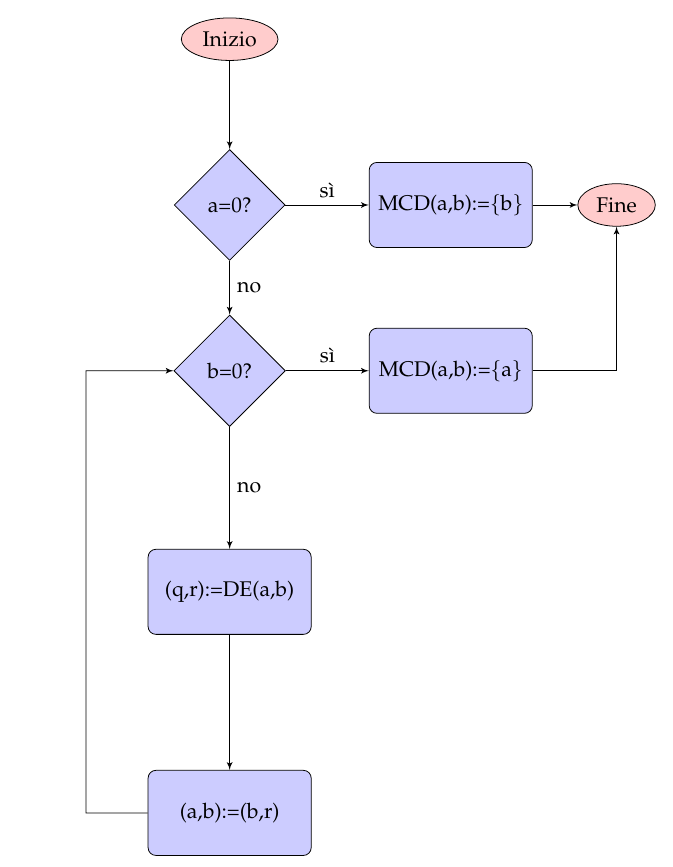
\includegraphics[scale=.55]{res/Algo_euclideo.png}
	\captionof{figure}{Algoritmo euclideo delle divisioni successive}
\end{center}

\subsection{Equazioni diofantee}\index{Equazione!Diofantea}

Oltre al calcolo dei massimi comun divisori, l’algoritmo euclideo permette di risolvere un altro importante problema.

\begin{defbox}{Equazione diofantea}
	Un’\textbf{equazione diofantea} è un’equazione in cui appaiano solo indeterminate e numeri interi che si intenda risolvere in $\mathbb{Z}$, cioè per la quale siano ammesse come soluzioni solo numeri interi.
\end{defbox} 

Ci occupiamo qui di un particolare tipo di equazione diofantea: quella cosiddetta lineare a due indeterminate, cioè una equazione diofantea della forma:
\begin{equation}\label{eq:diofantea}
	ax+by=c
\end{equation}

dove $a,b,c \in \mathbb{Z}$. Risolvere l'equazione \ref{eq:diofantea} significa trovare le coppie di interi $(u,v)$ tali che rendano vera l'uguaglianza se sostituiti a $x$ e $y$, cioè tali che $au+bv=c$. La \ref{eq:diofantea} può anche non ammettere soluzioni. Ad esempio, l'equazione $0x+0y=1$ non ammette ovviamente soluzioni. Facendo uso della terminologia introdotta sopra, è chiaro che \ref{eq:diofantea} ammette soluzioni (intere) se e solo se $c$ è combinazione lineare di $a$ e $b$ a coefficienti in $\mathbb{Z}$. Ciò permette di dimostrare la prima importante osservazione su questo genere
di equazioni.

\begin{teorbox}[di Bezout]\label{thm:bezout}\index{Bezout}
	Sono equivalenti le seguenti affermazioni:
	\begin{enumerate}
		\item Siano $a,b$ numeri interi relativi non nulli. Allora esiste un massimo comune divisore $d$ di $a$ e $b$ e risulta $d = au+bv$ per opportuni interi $u,v$.
		\item Siano $a,b \in \mathbb{Z}$ e sia $d = MCD(a,b)$. Allora l'insieme $\{\alpha a + \beta b \; | \; \alpha, \beta \in \mathbb{Z}\}$ delle combinazioni lineari di $a$ e $b$ a coefficienti in $\mathbb{Z}$ coincide con l'insieme $d\mathbb{Z}=\{dk \; | \; k \in \mathbb{Z}\}$ dei multipli di $d$ in $\mathbb{Z}$.
		\item Preso $d= MCD(a,b)$, l'equazione diofantea $ax+by=c$ ha soluzioni se e solo se $d \divides c$.
		\item Due numeri interi $a,b$ si dicono coprimi se e solo se 1 è combinazione lineare $a$ e $b$.
	\end{enumerate}
\end{teorbox}

\begin{proof}
\begin{enumerate}
	\item Ovvio, mediante l'algoritmo delle divisioni successive è possibile ricavare un'espressione di $d$ come combinazione lineare $au+bv$.
	\item Dal punto precedente sappiamo che $d=au+bv$. Quindi $d \in \{\alpha a + \beta b \; | \; \alpha, \beta \in \mathbb{Z}\}$. Moltiplicando $d$ per un qualunque $k \in \mathbb{Z}$ si ottiene quindi:
	\begin{align*}
		kd = a (\alpha k) + b (\beta k) \in \{\alpha a + \beta b \; | \; \alpha, \beta \in \mathbb{Z}\}
	\end{align*}
Quindi $d\mathbb{Z} \subseteq \{\alpha a + \beta b \; | \; \alpha, \beta \in \mathbb{Z}\}$. Analogamente abbiamo visto che una combinazione lineare di $a$ e $b$ è esprimibile come multiplo di $d$, quindi vale anche l'inclusione inversa e i due insiemi coincidono,
\item Supponiamo che l'equazione abbia soluzioni. Allora esistono $u,v \in \mathbb{Z}$ tali che $au+bv=c$, dunque $c$ è combinazione lineare di $a$ e $b$ a coefficienti in $\mathbb{Z}$, e quindi, per il punto precedente, è un multiplo di $d=MCD(a,b)$. Per definizione di multiplo ovviamente sappiamo che $d$ divide $c$. Dunque, se supponiamo che $d$ non divida $c$ dobbiamo trarre la conclusione che la nostra equazione non abbia soluzioni.
\item Non ha bisogno di dimostrazioni, è una definizione.
\end{enumerate}	
\end{proof}
\begin{lemmabox}[di Euclide]\index{Euclide}\label{lemma:euclide}
	Siano $a,b \in \mathbb{Z}$ coprimi. Se $c$ è un numero intero tale che $a \divides bc$ allora $a \divides c$.
\end{lemmabox}

\begin{proof}
	Per il teorema di Bezout esistono $u,v \in \mathbb{Z}$ tali che $1=au+bv$. D'altra parte $a$ divide $bc$ quindi $bc=ah$ per un opportuno numero intero $h$. Pertanto:
	\begin{align*}
		c &= c(au+bv) \\
		&= cau+cbv \\
		&= cau +ahv \\
		&= a(cu+hv)
	\end{align*}
	e quindi $a$ divide $c$.
\end{proof} 

\begin{example}
	Supponiamo di voler trovare soluzioni dell'equazione diofantea $74x+22y=10$. In questo caso è evidente che $MCD(74,22)=2$ e poiché $2 \divides 10$ siamo certi che l'equazione ammette soluzioni. Eseguendo le divisioni successive si ottiene:
	\begin{align*}
		74 &= 3 \cdot 22 + 8 \\
		22 &= 2 \cdot 8 + 6 \\
		8 &= 1 \cdot 6 + 2 \\
		6 &= 3 \cdot 2
	\end{align*}
	fino ad ottenere $2$ come ultimo resto non nullo. A questo punto possiamo esprimere i resti:
	\begin{align*}
		8 &= 74 - 3 \cdot 22 \\
		6 &= 22 - 2 \cdot 8 \\
		2 &= 8 - 1 \cdot 6
	\end{align*}
	e scrivere 2 come combinazione lineare di 74 e 22:
	\begin{align*}
		2 &= 8 - 6 & \\
		&= 8 - (22- 2 \cdot 8) & \text{\textcolor{gray}{(Sostituendo 6)}}\\
		&= 8 - 22 + 2 \cdot 8 \\
		&= 8 (1+2) - 22 &  \text{\textcolor{gray}{(Raccogliendo i coefficienti di 8)}}\\
		&= 3 \cdot 8 -22 \\
		&= 3 \cdot (74 - 3 \cdot 22) - 22 & \text{\textcolor{gray}{(Sostituendo 8)}} \\
		&= 3 \cdot 74 - 9 \cdot 22 - 22 \\
		&= 3 \cdot 74 - 10 \cdot 22 \\
		&= 3 \cdot 74 + (-10) \cdot 22
	\end{align*}
	Abbiamo così trovato che $2$ è esprimibile come combinazione lineare $\alpha 74 + \beta 22$ con $\alpha=3$ e $\beta=-10$. La coppia $(3,-10)$ è soluzione dell'equazione diofantea $74x+22y=2$. Moltiplicando per $5$ si ottiene $75 (15) + 22(-50) =10$, dunque la coppia $(15,-50)$ è la soluzione dell'equazione diofantea $74x+22y=10$.
\end{example}

\subsection{Struttura quoziente}\label{sez:congruenze}\index{Struttura!Quoziente}
Siano $S$ un insieme non vuoto, e $\bot: S \times S \longrightarrow S$ un'operazione in $S$.

\begin{defbox}{Compatibilità}
	Una relazione di equivalenza $\mathfrak{R} \in Eq(S)$ si dice \textbf{compatibile a sinistra} con $\bot$ se:
	\begin{displaymath}
		\forall x_{1},x_{2} \in S \Biggl((x_{1}\ \mathfrak{R} \ x_{2}) \implies \Bigl(\forall a \in S \bigl(a \bot x_{1} \ \mathfrak{R} \ a \bot x_{2}\bigr)\Bigr)\Biggr)
	\end{displaymath}
	Analogamente, $\mathfrak{R}$ si dice \textbf{compatibile a destra} con l'operazione $\bot$ se:
	\begin{displaymath}
		\forall x_{1},x_{2} \in S \Biggl((x_{1}\ \mathfrak{R} \ x_{2}) \implies \Bigl(\forall a \in S \bigl( x_{1} \bot a \ \mathfrak{R} \ x_{2} \bot a \bigr)\Bigr)\Biggr)
	\end{displaymath}
\end{defbox}

\begin{defbox}{Congruenza}\index{Congruenza}
	Sia $(S,\bot)$ una struttura algebrica. Una relazione di equivalenza $\mathfrak{R}$ in $S$ si dice una \textbf{congruenza} in $(S,\bot)$ se qualunque siano gli elementi $x_{1},x_{2},y_{1},y_{2}$ di $S$ tali che $x_{1} \ \mathfrak{R} \ x_{2}$ e $y_{1} \ \mathfrak{R} \ y_{2}$, risulta anche:
	\begin{displaymath}
		x_{1} \bot y_{1} \ \mathfrak{R} \ x_{2} \bot y_{2}
	\end{displaymath}
\end{defbox}


Pertanto, quando $\mathfrak{R}$ è una congruenza in $(S,\bot)$, e solo allora, è possibile considerare l'applicazione:
\begin{displaymath}
	\bot_{\mathfrak{R}}: ([x]_{\mathfrak{R}},[y]_{\mathfrak{R}}) \mapsto [x \bot y]_{\mathfrak{R}} \in S/{\mathfrak{R}}
\end{displaymath}
Tale applicazione è un'operazione nell'insieme quoziente $S/{\mathfrak{R}}$, chiamata \textbf{operazione quoziente} di $\bot$ rispetto a $\mathfrak{R}$. La struttura $(S/{\mathfrak{R}}, \bot_{\mathfrak{R}})$ viene chiamata \textbf{struttura quoziente}.


\begin{propbox}\label{prop:operazione_quoziente}
	Siano $S$ un insieme non vuoto, $\bot: S \times S \rightarrow S$ un'operazione in $S$ e $\mathfrak{R}$ una congruenza in $(S,\bot)$. Si ha:
	\begin{itemize}
		\item Se $\bot$ è associativa, allora anche $\bot_{\mathfrak{R}}$ è associativa;
		\item Se $\bot$ è commutativa, allora anche $\bot_{\mathfrak{R}}$ è commutativa;
		\item Se $u$ è un elemento neutro in $(S,\bot)$ allora $[u]_{\mathfrak{R}}$ è elemento neutro in $(S/{\mathfrak{R}},\bot_{\mathfrak{R}})$.
		\item Se $x$ è un elemento simmetrizzabile di $(S,\bot)$ e $x'$ è un suo simmetrico, allora $[x]_{\mathfrak{R}}$ è un elemento simmetrizzabile di $(S/{\mathfrak{R}},\bot_{\mathfrak{R}})$ e $[x']_{\mathfrak{R}}$ è un suo simmetrico.
	\end{itemize}
\end{propbox}

\begin{osservation}
	Una relazione di equivalenza $\mathfrak{R}$ è una congruenza in $(S,\bot_{1},\ldots,\bot_{n})$ se e soltanto se è compatibile con tutte le operazioni $\bot_{i}$ per ogni $i \in \{1, \ldots, n\}$.
\end{osservation}

\section{Congruenze in $\mathbb{Z}$}

\subsection{La relazione di congruenza modulo m}

Sia $m$ un numero intero relativo, e sia $\equiv_{m}$ la relazione binaria definita in $\mathbb{Z}$ ponendo:
\begin{equation}
	\forall a,b \in \mathbb{Z} \bigl(a \equiv_{m} b \iff m \divides (a-b)\bigr)
\end{equation}
ovvero se e solo se $a$ e $b$ sono numeri interi relativi tali che la differenza $(a-b)$ è multiplo di $m$, ovvero esiste $n \in \mathbb{Z}$ tale che $a-b=nm$.

Qualunque sia $a \in \mathbb{Z}$ risulta $a-a=0=0 \cdot m$, e quindi $a \equiv_{m} a$ e la relazione $\equiv_{m}$ risulta riflessiva. Siano $a,b$ numeri interi tali che $a \equiv_{m} b$. Allora risulta $a-b=km$ con $k \in \mathbb{Z}$, e quindi $b-a=-(a-b)=(-k)m$, sicché $b \equiv_{m} a$ e la relazione $\equiv_{m}$ è anche simmetrica. Siano infine $a,b,c$ numeri interi tali che $a \equiv_{m} b$ e $b \equiv_{m} c$. Allora esistono $h,k \in \mathbb{Z}$ tali che $a-b = km$ e $b-c=km$, sicché:
\begin{displaymath}
	a-c = (a-b)+(b-c) = hm+km=(h+k)m
\end{displaymath}
e quindi $a \equiv_{m} c$, e $\equiv_{m}$ è transitiva. Pertanto $\equiv_{m}$ \emph{è una relazione di equivalenza} in $\mathbb{Z}$. Se $a,b \in \mathbb{Z}$ sono due interi tali che $a \equiv_{m} b$ è possibile trovare usata la notazione $a \equiv b \ (mod. \ m)$.

Se $a$ è un numero intero relativo, la classe di equivalenza di $a$ rispetto alla relazione $\equiv_{m}$ si chiama ``\textbf{classe di congruenza} di $a$ modulo $m$'' e si denota col simbolo $[a]_{m}$. Un numero intero $b$ appartiene ad $[a]_{m}$ se e solo se $b \equiv_{m} a$, e quindi e se solo se $b-a=km$ per qualche $k \in \mathbb{Z}$. Pertanto:
\begin{displaymath}
	[a]_{m} = \{a +km \; | \; k \in \mathbb{Z}\}
\end{displaymath}
e in particolare:
\begin{displaymath}
	[0]_{m} = \{km \; | \; k \in \mathbb{Z}\} = m\mathbb{Z}
\end{displaymath}
dove $m\mathbb{Z}$ è l'insieme dei multipli di $m$. L'insieme quoziente $\mathbb{Z}/{\equiv_{m}}$ di $\mathbb{Z}$ rispetto alla relazione di equivalenza $\equiv_{m}$ si denota col simbolo $\mathbb{Z}_{m}$, e si chiama \textbf{insieme delle classi di interi modulo $m$}.

\begin{osservation}
	Poiché in $\mathbb{Z}$ l'unico multiplo di 0 è 0, si ha subito che la relazione $\equiv_{0}$ coincide con la relazione identica. D'altra parte ogni numero intero è divisibile per 1, sicché la relazione $\equiv_{1}$ è la relazione totale, e quindi $|\mathbb{Z}_{1}|=1$. È inoltre chiaro che per ogni intero relativo $m$ la relazione $\equiv_{m}$ e la relazione $\equiv_{-m}$ coincidono. Queste considerazioni consentono di limitare la nostra analisi al caso degli $m>1$.
\end{osservation}

\begin{example}
	Si consideri in $\mathbb{Z}$ la relazione di equivalenza $\equiv_{2}$. Due numeri interi $a,b \in \mathbb{Z}$ sono in relazione tra di loro se e solo se:
	\begin{displaymath}
		a \equiv_{2} b \iff 2 \divides (a-b) \iff \exists k \in \mathbb{Z} \bigl((a-b)=2k\bigr)
	\end{displaymath}
	ovvero se e soltanto se $(a-b)$ risulta un numero pari. Chiaramente la differenza tra due numeri interi è pari se e soltanto se $a$ e $b$ hanno la \textit{stessa parità} (entrambi pari oppure entrambi dispari). Infatti sia per assurdo $a$ un numero dispari e $b$ un numero pari della forma $2t$ per un opportuno $t \in \mathbb{Z}$. Essendo $a-b$ un numero pari esso sarà sicuramente della forma $2k$ per un qualche intero $k$.  Essendo $a$ un numero dispari questo può essere scritto nella forma $2n+1$ e si ha:
	\begin{displaymath}
		(a-b) = (2n+1)- 2t = 2n+1-2t= 2(n-t) + 1
	\end{displaymath}
	e $(a-b)$ risulterebbe un numero dispari, contro le nostre ipotesi.
\end{example}


\begin{example}
	Dati due numeri interi $x$ e $y$, diciamo che $x \equiv_{3} y$ se $(x-y)$ è multiplo di tre. Si vede subito che $0$ è congruo a tutti i multipli di tre. $1$ è congruo a tutti i numeri del tipo $\{\ldots, -5, -2, 1,4,7,10,\ldots\} = \{1+3k / k\in \mathbb{Z}\}$. $2$ è congruo a tutti i numeri del tipo $\{\ldots,-4,-1,2,5,8,11,\ldots\}=\{2+3k/k \in \mathbb{Z}\}$. Quindi nella partizione definita dalla congruenza modulo 3 ci sono tre classi di congruenza: $[0]_{3}, [1]_{3},[2]_{3}$.
\end{example}

\begin{propbox}
	Sia $m>1$ un numero intero. Qualunque sia il numero intero relativo $a$ risulta $a \equiv_{m} r$ dove $r$ è il resto della divisione euclidea di $a$ per $m$.
\end{propbox}

\begin{proof}
	Denotato con $q$ il quoziente della divisione euclidea di $a$ per $m$, si ha $a=mq+r$, con $0 \leq r < |m|$, per cui $(a-r) =mq$ e quindi $a \equiv_{m} r$.
\end{proof}


\begin{teorbox}
	Sia $m>1$ un numero intero. Allora $\mathbb{Z}_{m}$ è un insieme finito di ordine $m$ e risulta:
	\begin{displaymath}
		\mathbb{Z}_{m} = \{[0]_{m},[1]_{m},\ldots,[m-1]_{m}\}
	\end{displaymath}
\end{teorbox}


\begin{corolbox}
	Sia $m>1$ un numero intero, per ogni $a,b \in \mathbb{Z}$:
	\begin{displaymath}
		a \equiv_{m} b \iff \text{hanno lo stesso resto nella divisione euclidea per $m$}
	\end{displaymath}
\end{corolbox}

\begin{osservation}
	Si ha $m = 1 \cdot m + 0$ e quindi $m \equiv_{m} 0$. Ovvero $[m]_{m}=[0]_{m}$.
\end{osservation}

Per i risultati appena ottenuti possiamo vedere l'insieme quoziente $\mathbb{Z}_{m}$ come l'insieme delle \textbf{classi di resto modulo $m$}.


\begin{propbox}
	Le relazioni di congruenza sono compatibili con l'addizione. Dati i numeri interi $a,a',b,b' \in \mathbb{Z}$:
	\begin{equation}
	(a \equiv_{m} a' \land b \equiv_{m} b') \implies (a+b \equiv_{m} a'+b')
	\end{equation}
\end{propbox}

\begin{proof}
	Da $a \equiv_{m} a'$ e $b \equiv_{m} b'$ segue :
	\[
	\begin{cases}
		a-a' = km \\
		b-b' = hm
	\end{cases}
	\] per opportuni interi $h,k \in \mathbb{Z}$. Sommando membro a membro si ha:
	\begin{align*}
		a-a'+(b-b') = km+hm  \iff	a+b - (a'+b') = (h+k)m
	\end{align*}
	Quindi $a+b \equiv_{m} a'+b'$.
\end{proof}


\begin{propbox}
	Le relazioni di congruenza sono compatibili con la moltiplicazione. Dati i numeri interi $a,a',b,b' \in \mathbb{Z}$, vale:
	\begin{equation}
	(a \equiv_{m} a' \land b \equiv_{m} b') 	\implies	(a \cdot b \equiv_{m} a' \cdot b')
	\end{equation}
\end{propbox}

\begin{proof}
	È lasciata al lettore come esercizio.
\end{proof}

Da queste due proposizioni segue che:

\begin{teorbox}
	Qualunque sia il numero intero relativo $m$, la relazione di equivalenza $\equiv_{m}$ è una congruenza nella struttura algebrica $(\mathbb{Z},+,\cdot)$.
\end{teorbox}

È opportuno osservare che le uniche congruenze nella struttura algebrica $(\mathbb{Z},+,\cdot)$ sono le congruenze modulo $m$, al variare di $m \in \mathbb{Z}$. Questo teorema permette di introdurre nell'insieme $\mathbb{Z}_{m}$ delle classi di resto le operazioni quoziente dell'addizione e della moltiplicazione in $\mathbb{Z}$. Tali operazioni, denotate ancora con i simboli $+$ e $\cdot$, sono definite ponendo:
\begin{align*}
\begin{cases}
		[a]_{m}+[b]_{m} = [a+b]_{m}\\
	[a]_{m} \cdot [b]_{m} = [ab]_{m}
\end{cases}
\end{align*}
Tali operazioni sono associative e commutative, la classe $[0]_{m}$ è elemento neutro in $\mathbb{Z}_{m}$ rispetto all'addizione, mentre $[1]_{m}$ è elemento neutro rispetto alla moltiplicazione. Inoltre, per ogni numero intero relativo $a$, la classe $[a]_{m}$ è dotata di opposto in $\mathbb{Z}_{m}$ e risulta $-[a]_{m}=[-a]_{m}$. Infine, qualunque siano i numeri interi relativi $a,b,c \in \mathbb{Z}$ risulta:
\begin{align*}
	([a]_{m}+[b]_{m})[c]_{m} &=[a+b]_{m}[c]_{m} \\
	&=[(a+b)c]_{m}\\
	&=[ac+bc]_{m}\\
	&=[ac]_{m} + [bc]_{m}\\
	&=[a]_{m}[c]_{m} + [b]_{m}[c]_{m}
\end{align*}
sicché in $\mathbb{Z}_{m}$ la moltiplicazione è distributiva rispetto all'addizione. La struttura $(\mathbb{Z}_{m},+,\cdot)$ risulta quindi un anello.
Osserviamo che in $\mathbb{Z}_{m}$ non vale in generale la legge di annullamento del prodotto, ovvero esistono dei quozienti in cui sono presenti divisori dello zero.


\begin{example}
	Ad esempio in $\mathbb{Z}_{6}$ gli elementi $[2]_{6}$, $[3]_{6}$ e $[4]_{6}$ risultano essere divisori dello zero:
	\begin{align*}
		[2]_{6} \cdot [3]_{6} = [6]_{6} = [0]_{6} = [12]_{6}=[4]_{6} \cdot [3]_{6}
	\end{align*}
	e $\mathbb{Z}_{6}$ non risulta essere un anello integro, in particolare un dominio di integrità.
\end{example}


\begin{teorbox}
	Sia $m>1$ un numero intero relativo. Allora in $\mathbb{Z}_{m}$ vale la legge di annullamento del prodotto se e solo se $m$ è primo.
\end{teorbox}

\begin{propbox}\label{prop:invertibili_zm}
	Siano $a \in \mathbb{Z}$, $n \in \mathbb{N}^{*}$. $[a]_{m}$ è invertibile in $\mathbb{Z}_{m}$ se, e solo se, $a$ ed $m$ sono coprimi.
\end{propbox}

\begin{proof}Abbiamo:
\begin{itemize}
	\item[$\implies$] Se $[a]_{m}$ è invertibile, esiste $[b]_{m}$ tale che:
	\begin{displaymath}
		[a]_{m}\cdot[b]_{m} = [ab]_{m}=[1]_{m}
	\end{displaymath}
	Quindi: $$m \divides (1-ab) \iff \exists h \in \mathbb{Z} \bigl(1-ab = hm\bigr)$$ 
	Da $1=ab+hm$ e dal Teorema di Bezout segue che $a$ ed $m$ sono coprimi.
	
	\item[$\impliedby$] Viceversa, supposti $a$ ed $m$ coprimi tra di loro, essendo $(a,m)=1$ esistono $\alpha,\beta$ tali che $1=\alpha a + \beta m$. 
	
	Da $\alpha a-1 = -\beta m$ segue allora $\alpha a \equiv_{m} 1$ per cui $[\alpha a]_{m} = [\alpha]_{m} [a]_{m}$ e $[\alpha]_{m}$ è l'inverso di $[a]_{m}$.
\end{itemize}
\end{proof}


\begin{corolbox}
	Siano $a \in \mathbb{Z}$, $n \in \mathbb{N}^{*}$ e sia $[a]_{m} \neq [0]_{m}$. Allora $[a]_{m}$ è un divisore dello zero in $\mathbb{Z}_{m}$ se, e solo se, $a$ ed $m$ non sono coprimi.
\end{corolbox}

\begin{proof} Si ha:
	\begin{itemize}
		\item[$\implies$] Se $[a]_{m}$ è un divisore dello zero risulta non regolare e quindi non invertibile. Per la proposizione precedente allora $a$ ed $m$ non sono coprimi. 
		
		\item[$\impliedby$] Viceversa, se $d=(a,m)$ risulta $1<d<m$ ed esistono $a_{1},m_{1}$ tali che $a=a_{1}d$ ed $m=m_{1}d$. Dall'essere $1<n_{1}<n$ segue $[m_{1}]_{m} \neq [0]_{m}$ e $[a]_{m}[m_{1}]_{m} = [a_{1}dm_{1}]_{m} = [a_{1}]_{m}[m]_{m} = [a_{1}][0]_{m}= [0]_{m}$, per cui $[a]_{m}$ è un divisore dello zero.
	\end{itemize}
\end{proof}

\begin{corolbox}
	Siano $a \in \mathbb{Z}$ ed $m \in \mathbb{N}^{*}$ sia $[a]_{m} \neq [0]_{m}$. Allora $[a]_{m}$ è invertibile se e solo se non è un divisore dello 0.
\end{corolbox}

\begin{teorbox}[Caratterizzazione anello degli interi modulo $m$]\label{thm:car_anelli_zm}
	Sia $m>1$ un intero. Allora le seguenti affermazioni sono equivalenti:
	\begin{enumerate}
		\item l'anello $\mathbb{Z}_{m}$ è un campo;
		\item L'anello $\mathbb{Z}_{m}$ è un dominio di integrità;
		\item $m$ è un numero primo.
	\end{enumerate}
\end{teorbox}

\begin{proof}
	Le condizioni $(1)$ e $(2)$ sono equivalenti per il Corollario precedente. Per dimostrare l'equivalenza di $(1)$ e $(3)$ si osservi che, se $m$ è primo, tutti gli interi $1, \ldots, m-1$ sono coprimi con $m$ e quindi tutte le classi $[1]_{m},[2]_{m},\ldots [m-1]_{m}$ sono invertibili. Viceversa, supposto che $\mathbb{Z}_{m}$ sia un campo, se $m$ non fosse primo esisterebbe un divisore $m_{1}$ di $m$ tale che $1 < m_{1} < m$. Allora risulterebbe $[m_{1}]_{m} \neq [0]_{m}$ ed $[m_{1}]_{m}$ non invertibile, essendo $(m,m_{1}) = m_{1}>1$. Dall'assurdo segue che $m$ è necessariamente primo.
\end{proof} 


\begin{corolbox}
	Gli elementi non nulli di $\mathbb{Z}_{m}$ sono tutti invertibili se e solo se $m$ è primo.
\end{corolbox}

\subsubsection{Periodo di un elemento}\index{Periodo}
Il concetto di classe di resto ha a che fare con la nozione di periodo di un elemento in un gruppo. Ricordiamo che, se un gruppo $G$ è denotato con la notazione additiva, allora il concetto di potenza coincide con il concetto di multiplo. Quindi si dice che $G$ è ciclico se esiste $a \in G$ tale che $G=\langle a \rangle = \{na / n \in \mathbb{Z}\}$.

\begin{lemmabox}
	Sia $G=\langle x \rangle$ un gruppo ciclico. Allora $G$ è finito se e solo se esiste un numero intero positivo $m$ tale che $x^{m}=1$.
\end{lemmabox}

\begin{proof}
	Se $G$ è finito, esistono dei numeri interi positivi $h$ e $k$ tali che $x^{h}=x^{k}$. Supposto, per fissare le idee, $h>k$, si ha $m=h-k>0$ e $x^{m}=x^{h-k}=x^{h}(x^{k})^{-1}=1$. Reciprocamente, esista un numero intero positivo $m$ tale che $x^{m}=1$. Qualunque sia il numero intero relativo $n$, si ha per il teorema della divisione euclidea: $n=mq+r$, con $q$ ed $r$ numeri interi relativi tali che $0\leq r < m$. Allora $x^{n}= x^{mq+r}=(x^{m})^{q}x^{r}=x^{r}$. Per cui $G=\{x^{0},x^{1},\ldots,x^{m-1}\}$ è finito.
\end{proof}


\begin{teorbox}[Teorema ponte]
	Sia $G=\langle x \rangle$ un gruppo ciclico finito di ordine $m$. Allora $G=\{x^{0},x^{1},\ldots,x^{m-1}\}$ ed $m$ è minimo intero positivo tale che $x^{m}=1$.
\end{teorbox}

\begin{defbox}{Elemento periodico}\index{Elemento!Periodico}
	Sia $G$ un gruppo. Un elemento $x \in G$ si dice \textbf{periodico} se il sottogruppo $\langle x \rangle$ è finito. In questo caso l'ordine di $\langle x \rangle$ si chiama \textbf{periodo} di $x$ e si denota con il simbolo $o(x)$. Un gruppo $G$ si dice \textbf{periodico} se ogni suo elemento è periodico.
\end{defbox}

\begin{osservation}
	Un elemento $x$ di $G$ è periodico se e solo se esiste $m \in \mathbb{Z}$ tale che $x^{m}=1_{G}$ se $G$ è denotato moltiplicativamente. Nel caso in cui $G$ è denotato additivamente allora $x \in G$ è periodico se $mx = 0_{G}$.
\end{osservation}

\begin{lemmabox}
	Sia $(G,\cdot)$ un gruppo e $x \in G$ un elemento periodico di periodo $n$. Allora:
	\begin{displaymath}
		\forall a \in \mathbb{Z} \bigl(x^{a} = x^{rest(a,n)}\bigr)
	\end{displaymath}
	dove $rest(a,n)$ è il resto della divisione euclidea di $a$ per $n$.
\end{lemmabox}
\begin{proof}
	Sia $r=rest(a,n)$ allora esiste un $k \in \mathbb{Z}$ tale che $a=kn+r$. Allora:
	\begin{align*}
		x^{a} &= x^{kn+r}\\
		&= (x^{n})^{k} \cdot x^{r}\\
		&= 1_{G}  \cdot x^{r} = x^{r}
	\end{align*}
	e l'asserto è dimostrato.
\end{proof}

\begin{propbox}
	Sia $(G,\cdot)$ un gruppo e $x \in G$ un elemento periodico di periodo $n$. Allora:
	\begin{displaymath}
		\forall a,b \in \mathbb{Z} \bigl(x^{a} = x^{b} \iff a \equiv_{n} b \iff rest(a,n) = rest(b,n)\bigr)
	\end{displaymath}
\end{propbox}
\begin{proof}
\begin{itemize}
		\item[$\impliedby$] Se $a \equiv_{m} b$ allora $m \divides (a-b)$. Ovvero $(a-b)= q m$ per un opportuno $q \in \mathbb{Z}$. Allora $a= q m+ b$ e risulta:
	\begin{displaymath}
		x^{a} = x^{qm +b} = (x^{m})^{q} \cdot x^{b} = (1_{G}) \cdot x^{b} = x^{b}
	\end{displaymath}
	\item[$\implies$] Se $x^{a} = x^{b}$ allora $x^{a-b}=1_{G} = x^{0}$ e quindi vale $a \equiv_{m} b$.
\end{itemize}
\end{proof}

\begin{defbox}{Funzione di Eulero}\index{Funzione di Eulero}
	La funzione $\varphi$ di Eulero è l'applicazione di $\mathbb{N}^{*}$ in sè definita ponendo, per ogni $n \in \mathbb{N}^{*}$:
	\begin{equation}
		\varphi(n)=|\{a \in \mathbb{N}^{*} \; | \; a \leq n \land MCD(a,n)=1 \}|
	\end{equation}
	ovvero il numeri degli interi positivi minori di $n$ e primi con $n$.
	
\end{defbox}

\begin{example}
	Ad esempio, poiché tra gli interi positivi $1,2,3,4,5,6$ ad essere coprimi con $6$ sono solo $1$ e $5$ si ha $\varphi(6)=2$.
\end{example}

La funzione di Eulero esprime la cardinalità del gruppo degli invertibili dei quozienti di $\mathbb{Z}$. Infatti, per ogni $n \in \mathbb{N}^{*}$, sappiamo che gli elementi dell'anello $\mathbb{Z}_{n}$ corrispondono precisamente ai numeri interi positivi tali che $a \leq n$, nel senso che:
\begin{displaymath}
	\mathbb{Z}_{n} = \{[a]_{n} \; | \; a \in \mathbb{N}^{*} \land a \leq n \}
\end{displaymath}

e se $a$ e $b$ sono interi positivi minori o uguali a $n$ si ha $[a]_{n} = [b]_{n}$ se e solo se $a=b$. Sappiamo inoltre che, con queste stesse notazioni, $[a]_{n}$ è invertibile in $\mathbb{Z}_{n}$ se e solo se $a$ ed $n$ sono coprimi. Dunque:

\begin{displaymath}
	\mathcal{U}(\mathbb{Z}_{n}) = \{[a]_{n} \; | \; a \in \mathbb{N}^{*} \land a \leq n \land MCD(a,n) = 1\}
\end{displaymath}
ovvero:

\begin{displaymath}
	|\mathcal{U}(\mathbb{Z}_{n})|=\varphi(n)
\end{displaymath}

\begin{example}
	Il gruppo composto dall'insieme finito $\mathbb{Z}_{4}=\{[0]_{4},[1]_{4},[2]_{4},[3]_{4}\}$ insieme all'operazione di addizione è un gruppo ciclico in quanto esiste un elemento generatore in grado di generare tutti gli elementi di $\mathbb{Z}_{4}$. Infatti, preso $[1]_{4}$ si ha:
	\begin{displaymath}
		\begin{array}{l}
			([1]_{4})^{1} = 1 \cdot [1]_{4} =[1 \cdot 1]_{4} = [1]_{4}\\
			([1]_{4})^{2} = 2 \cdot [1]_{4} =[2 \cdot 1]_{4} = [2]_{4}\\
			([1]_{4})^{3} = 3 \cdot [1]_{4} =[3 \cdot 1]_{4} = [3]_{4}\\
			([1]_{4})^{4} = 4 \cdot [1]_{4} =[4 \cdot 1]_{4} = [4]_{4} = [0]_{4}\\
		\end{array}
	\end{displaymath}
	Il periodo dell'elemento $[1]_{4}$ è uguale a quattro, infatti, il sottogruppo generato da $[1]_{4}$, ovvero l'insieme $\langle [1]_{4} \rangle = \{n [1]_{4} / n \in \mathbb{Z}\} = \{[0]_{4},[1]_{4},[2]_{4},[3]_{4}\}$ coincide con l'insieme $\mathbb{Z}_{4}$. L'elemento $[2]_{4}$ non è un generatore perché i suoi multipli (potenze) non generano tutti gli altri elementi dell'insieme $\mathbb{Z}_{4}$:
	\begin{displaymath}
		\langle [2]_{4} \rangle = \{[0]_{4},[2]_{4}\}
	\end{displaymath}
	Il periodo dell'elemento $[2]_{4}$ è 2 perché il numero intero più piccolo $k$ tale che $2^{k} = 0_{\mathbb{Z}_{4}}$ è $k=2$. Infatti:
	\begin{displaymath}
		([2]_{4})^{2} = [2]_{4}+[2]_{4} = [4]_{4} = [0]_{4}
	\end{displaymath}
	Anche l'elemento $[3]_{4}$ è un generatore del gruppo ciclico in quanto il sottogruppo $\langle [3]_{4} \rangle $ coincide con $\mathbb{Z}_{4}$:
	\begin{displaymath}
		\langle [3]_{4} \rangle = \{[0]_{1},[2]_{4},[3]_{4}\}
	\end{displaymath}
	Il periodo di $[3]_{4}$ risulta quindi uguale a quattro perché sono necessarie quattro ripetizioni dell'operazione per avere l'elemento neutro $([3]_{4})^{4}=[0]_{4}$. Quindi $\mathbb{Z}_{4}$ ha due generatori ($[1]_{4}$ e $[3]_{4}$) e vale:
	\begin{displaymath}
		\langle [1]_{4} \rangle = \langle [3]_{4} \rangle = \mathbb{Z}_{4}
	\end{displaymath}
	notiamo inoltre che $1$ e $3$ sono coprimi con $4$ e vale $\varphi(4)=2$. Infatti, il numero di generatori distinti di un gruppo ciclico di ordine $m$ coincide con il numero di interi positivi strettamente minori di $m$ e coprimi con $m$, ovvero $\varphi(m)$.
\end{example}

A conclusione di questa trattazione sulle proprietà dei gruppi ciclici vogliamo mostrare che, a meno di isomorfismi, \emph{gli unici gruppi ciclici finiti}, ovvero i gruppi per i quali esiste un elemento $x$ tale che $x^{m}=1$, \emph{sono i gruppi additivi} $(\mathbb{Z}_{m},+)$. Infatti, considerato un gruppo ciclico finito $G$ e l'applicazione $f: n \in \mathbb{Z} \rightarrow x^{n} \in G$, poiché $G=\{x^{n} / n \in \mathbb{Z}\}$ si ha che $f$ è suriettiva. Qualunque siano gli elementi $m,n \in \mathbb{Z}$ si ha inoltre:
\begin{displaymath}
	f(m+n)= x^{m+n}=x^{m}+x^{n}=f(m)+f(n)
\end{displaymath}
ed $f$ risulta essere un epimorfismo. Dal Teorema di omomorfismo segue allora che $G$ è isomorfo a $\mathbb{Z}/{\mathfrak{R}_{f}}$ dove $\mathfrak{R}_{f}$ è nucleo di equivalenza di $f$. Se $|G|=m$ si ha $\mathfrak{R}_{f}$ è equivalente\footnote{Si tenga sempre a mente che $f$ è una applicazione che associa ogni intero $n$ alla potenza $x^{n} \in G$. Se $G$ è un gruppo ciclico denotato additivamente allora $f$ è definita ponendo $n \mapsto nx$.} a $\equiv_{m}$ e $G$ è isomorfo a $\mathbb{Z}_{m}$.

\begin{corolbox}
	L'anello $(\mathbb{Z}_{m},+,\cdot)$ ha caratteristica pari ad $m$.
\end{corolbox}
\begin{proof}
	Per ogni $a \in \mathbb{Z}$:
	\begin{displaymath}
		[a]_{m} = [0]_{m} \iff a \equiv_{m} 0 \iff m \divides (a-0) \iff m \divides a \iff a =km
	\end{displaymath}
	ed $m$ risulta essere la caratteristica dell'anello $\mathbb{Z}_{m}$.
\end{proof}

\subsection{Equazioni congruenziali}\index{Equazioni!Congruenziali}
Nel paragrafo precedente è stata data una condizione necessaria e sufficiente affinché una classe $[a]_{m} \neq [0]_{m}$ sia invertibile. In questa sezione si vedrà come è possibile determinare $[a]_{m}^{-1}$ quando $[a]_{m}$ è invertibile\footnote{Ovvero quando $a$ ed $m$ sono coprimi.}.

Si ricordi che un elemento $[a]_{m}$ è invertibile in $\mathbb{Z}_{m}$ quando esiste $[c]_{m} \in \mathbb{Z}_{m}$ tale che: $[a]_{m}[c]_{m}=[ac]_{m}=[1]_{m}$ ovvero se esiste $c \in \mathbb{Z}$ tale che $ac \equiv_{m} 1$. In generale vale la seguente definizione:

\begin{defbox}{Equazioni congruenziali}
	Siano $a,b,m \in \mathbb{Z}$ e sia $m>1$. L'espressione	$ax \equiv_{m} b$ si dice \textbf{equazione congruenziale} di termini $a$ e $b$ modulo $m$. Un numero intero relativo $c$ si dice \textbf{soluzione} dell'equazione congruenziale $ax \equiv_{m} b$ se risulta $ac \equiv_{m} b$. Ciò equivale a richiedere che sia $[a]_{m}[c]_{m} = [b]_{m}$.
\end{defbox}

\begin{osservation}
	Un elemento $[a]_{m} \in \mathbb{Z}_{m}$ è invertibile se, e solo se, l'equazione congruenziale $ax \equiv_{m} 1$ ammette una soluzione.
\end{osservation}

\begin{propbox}[Criterio di compatibilità]
	Siano $a,b, m \in \mathbb{N}^{*}$, $d=MCD(a,m)$. L'equazione congruenziale $ax \equiv_{m} b$ ha soluzione se, e solo se, $d$ divide $b$.
\end{propbox}

\begin{proof}Dimostriamo le due implicazioni:
\begin{itemize} 
	\item[$\implies$] Se $c$ è una soluzione dell'equazione congruenziale allora $\exists k \in \mathbb{Z}$ tale che $ac-b=km$. Allora da $d \divides a$ e $d \divides m$ segue $d \divides ac-km = b$.
	
	\item[$\impliedby$] Viceversa, si supponga $d$ divisore di $b$: esiste $h \in \mathbb{Z}$ tale che $b=dh$. Essendo inoltre $d$ un massimo comune divisore tra $a$ ed $m$, esistono degli interi $r$ ed $s$ tali che $d=ra+sm$. Da ciò segue $b=hd=h(ra+sm)$. In particolare, da $hra-b=-hsm$ segue che $hr$ è una soluzione dell'equazione congruenziale.
\end{itemize}
\end{proof}

\begin{propbox}
	Siano $a,b \in \mathbb{Z}$, $m \in \mathbb{N}^{*}$, $t$ un divisore comune di $a,b,m$. Allora le soluzioni dell'equazione congruenziale $ax \equiv_{m} b$ sono tutte e sole quelle dell'equazione congruenziale:
	\begin{displaymath}
		\frac{a}{t} x \equiv_{\frac{m}{t}} \frac{b}{t}
	\end{displaymath}
\end{propbox}

\begin{proof}
	È sufficiente osservare che, se $c$ è un intero, allora:
	\begin{align*}
		m &= t \cdot \frac{m}{t} \divides ac-b = t \cdot \frac{a}{t} \cdot c-t \cdot \frac{b}{t} \iff \frac{m}{t} \divides \frac{a}{t} \cdot c -\frac{b}{t}
	\end{align*}
\end{proof}

\begin{corolbox}
	Una congruenza compatibile $ax \equiv_{m} b$ ammette esattamente $d = MCD(a,m)$ soluzioni \textit{non congruenti} modulo $m$ date da:
	\begin{equation}
		x_{0} + k \frac{m}{d}
	\end{equation}
	dove $x_{0}$ è una soluzione della congruenza e $0 \leq k < d$.
\end{corolbox}

\begin{osservation}
	Se $MCD(a,m)=1$ allora la congruenza lineare ha un'unica soluzione.
\end{osservation}

\begin{propbox}
	Sia $c$ una soluzione dell'equazione congruenziale $ax \equiv_{m} 1$. Allora, se $b$ è un intero, $cb$ è soluzione dell'equazione congruenziale $ax \equiv_{m} b$.
\end{propbox}

\begin{proof}
	Basta osservare che, se $m$ divide $ac-1$, divide anche $(ac-1)b =acb-b$.
\end{proof}

\begin{propbox}
	Si consideri l'equazione congruenziale $ax \equiv_{m} b$ e siano $a$ ed $m$ primi tra loro. Allora l'equazione ha soluzioni, che costituiscono una classe di resto modulo $m$.
\end{propbox}

\begin{proof}
	Poiché $1=MCD(a,m)$ divide $b$ l'equazione ha soluzioni. Indicata con $c$ una di tali soluzioni, verifichiamo che l'insieme $X$ di tutte e sole le soluzioni dell'equazione coincide con $[c]_{m}$. Sia $y \in X$ una soluzione, da $ac \equiv_{m} b$ e $ay \equiv_{m} b$ segue:
	\begin{displaymath}
		ac \equiv_{m} ay \implies m \divides ac-ay = a (c-y)
	\end{displaymath}
	Ciò implica, essendo inoltre $m$ ed $a$ primi tra loro, che $m$ divide $c-y$, per cui $y \in [c]_{m}$. Viceversa, se $y \in [c]_{m}$, risulta $[c]_{m}=[y]_{m}$ e quindi $[a]_{m}[y]_{m}=[a]_{m}[c]_{m}=[b]_{m}$ come si voleva.
\end{proof}

\gbox{Tecniche di semplificazione}{red}{
	Data l'equazione congruenziale:
\begin{equation}\label{eq:congruenziale}
	ax \equiv_{m} c
\end{equation} dove $a,c,m \in \mathbb{Z}$ e $m \neq 0$:
\begin{enumerate}
	\item Se $a' \in [a]_{m}$ e $c' \in [c]_{m}$, l'equazione congruenziale $$a'x \equiv_{m} c'$$ è equivalente alla \ref{eq:congruenziale}.
	\item Per ogni $k \in \mathbb{Z}$, se $k \neq 0$, l'equazione congruenziale $$akx \equiv_{mk} ck$$ è equivalente alla \ref{eq:congruenziale}.
	\item Per ogni $t \in \mathbb{Z}$, se $t$ è coprimo con $m$, l'equazione congruenziale $$atx \equiv_{m} ct$$ è equivalente a \ref{eq:congruenziale}.
\end{enumerate}
}
\subsubsection{Esempi di equazioni congruenziali e loro soluzioni}
\begin{example}
	L'equazione $324x \equiv_{508} 127$ non ha soluzioni in quanto $MCD(324,508) \ndivides 127$.
\end{example}
\begin{example}
	L'equazione $120x \equiv_{m} 128$ ha soluzioni (4 è MCD tra 120 e 164 e divide 128). Troviamole. 
	
	Dividiamo tutto per 4: l'equazione diventa $30x \equiv_{41} 32$ che risulta essere una equazione congruenziale ridotta ai minimi termini in quanto 30 e 41 risultano essere coprimi. Eseguiamo l'algoritmo euclideo per risolvere l'equazione diofantea $1 = 30x + 41y$ si ottiene:
	\begin{align*}
		41 &= (1)30 + 11 \\
		30 &= (2)11 + 8 \\
		11 &=(1)8 + 3 \\
		8 &= (2)3+2 \\
		3 &=(1)2 +1 \\
		2 &=(2)1 +0
	\end{align*} 
Ricaviamo quindi le seguenti relazioni:
\begin{align*}
	11&=(1)41+(-1)30 \\
	8&=(1)30+(-2)11 \\
	3&=(1)11+(-1)8 \\
	2&=(1)8+(-2)3 \\
	1&=(1)3+(-1)2
\end{align*}
Dalle quali possiamo eseguire il seguente calcolo per ottenere una combinazione lineare di 30 e 41 che dia 1 come risultato:
\begin{align*}
	1 &= (1)3 +(-1)2 \\
	&=(1)3+(-1)\bigl(8+(-2)3\bigr)\\
	&= (-1)8 + (3)3 \\
	&=(-1)8 +(3)\bigl(11+(-1)8\bigr)\\
	&=(3)11 +(-4)8 \\
	&=(3)11+(-4)\bigl(30+(-2)11\bigr)\\
	&=(-4)30 + (11)11 \\
	&=(-4)30 + (11)\bigl(41 +(-1)30\bigr)\\
	&=(11)41 +(-15)30
\end{align*}
Pertanto, $1=(11 )\cdot 41 + (-15)\cdot 30$. Più significativamente: abbiamo scoperto che vale $(-15)30 \equiv_{41}  1$, cioè che l'inverso di $[30]_{41}$ in $\mathbb{Z}_{41}$ è $[-15]_{41}$. A questo punto sappiamo che l'unica classe in $\mathbb{Z}_{41}$ che, moltiplicata per $[30]_{41}$ dia $[32]_{41}$ è $([30]_{41})^{-1}[32]_{41}=[-15]_{41}[32]_{41} = [(-15)(32)]_{41}$. Questa classe è l'insieme delle soluzioni, in $\mathbb{Z}$, dell'equazione congruenziale originaria.
\end{example}

\begin{example}
	L'equazione $4x \equiv_{10} 8$ ha ovviamente 2 come soluzione in $\mathbb{Z}$. L’insieme di tutte le soluzioni non è $[2]_10$ ma $[2]_5$, perché in
	forma ridotta l’equazione diventa $2x \equiv_{5} 4$, notare: 2 e 5 sono coprimi. Si può osservare che, ad esempio, $7 \in [2]_{5} \setminus [2]_{10}$, quindi $[2]_{5}$ è strettamente contenuto in $[2]_{10}$; è facile anche verificare che $[2]_{5}$ è l’unione disgiunta di $[2]_{10}$ e $[7]_{10}$, quindi, l’equazione data, vista come equazione in $Z_{10}$: $[4]_{10} X = [8]_{10}$ ha esattamente due soluzioni: $[2]_{10}$ e $[7]_{10}$.
\end{example}

\begin{example}
	L’equazione $45x \equiv_{47} 476$ si risolve immediatamente senza bisogno di calcoli: evidentemente $45 \equiv_{47} -2$ e $476 \equiv_{47} 6$, quindi l’equazione è equivalente a (nel senso che ha le stesse soluzioni di) $-2x \equiv_{47} 6$, ovvero (dividendo -2 e 6 per -2, che è invertibile modulo 47) a $x \equiv_{47} -3$, che è già risolta: l’insieme delle soluzioni è $[-3]_{47}$.
\end{example}

\begin{example}
	L’equazione $32x - 4 \equiv_{18} 8$ non è altro che un modo diverso di scrivere $32x \equiv_{18} 12$. Per semplificarla possiamo dividere tutto per 2 (MCD tra 32 e 18), ottenendo $16x \equiv_{9} 6$. Da questa, siccome 2 è coprimo con 9, quindi invertibile modulo 9, dividendo 16 e 6 per 2 ricaviamo l’equazione equivalente $8x \equiv_{9} 3$; ma $8 \equiv_{9} -1$, quindi possiamo
	riscrivere questa come $-x \equiv_{9} 3$, ovvero $x \equiv_{9} -3$, e l’equazione originaria è risolta. In alternativa: da $32x \equiv_{18} 12$
	passiamo a $-4x \equiv_{18} 12$, perché $-4 \equiv_{18} 32$, quindi, dividendo tutto per 2, a $-2x \equiv_{9} 6$; possiamo ancora dividere -2
	per 2, o direttamente per -2, perché, di nuovo, 2 e -2 sono invertibili modulo 9, per ottenere ancora $x \equiv_{9} -3$ e così l’insieme $[-3]_{9}$ di tutte le soluzioni.
\end{example}


\begin{example}
	\begin{enumerate}
	\item Un esempio simile: $14x \equiv_{111} 21$ ha le stesse soluzioni di $2x \equiv_{111} 3$; qui bisogna fare attenzione al fatto che
	7, per il quale abbiamo diviso 14 e 21, e 111 sono coprimi. Come facciamo a saperlo? Be’, $111 \equiv_{7} 111 - 70 = 40$,
	siccome 42 è multiplo di 7 certamente non lo è 40 (infatti $40 \equiv_{7} -2$), quindi 7 non divide 111; poiché 7 è primo questo garantisce che 7 e 111 sono coprimi. A questo punto dobbiamo risolvere $2x \equiv_{111} 3$. Possiamo farlo usando l’algoritmo euclideo, oppure osservando che, siccome 3 è dispari come 111, allora $3 + 111$ è pari, ne ricaviamo l’intero $(3 + 111)/2 = 114/2 = 57$, allora $2 \cdot 57 = 3 + 111 \equiv_{57} 3$ e così vediamo che 57 è soluzione dell'equazione. Dal momento che l’equazione è ridotta (2 e 111 sono coprimi), l’insieme delle soluzioni è $[57]_{111}$.

	\item Si consideri l'equazione congruenziale:
	\begin{equation}
		ax \equiv_{m} b
	\end{equation}
	\paragraph{Caso A:} \textit{Risoluzione dell'equazione congruenziale del tipo:} $ax \equiv_{m} 1$ con $MCD(a,m)=1$.
	
	Essendo $1=MCD(a,m)$ è possibile determinare, mediante l'algoritmo di Euclide delle divisioni successive, degli interi $\alpha$ e $\beta$ tali che risulti $\alpha a + \beta m = 1$. L'intero $\alpha$ risulta essere una soluzione dell'equazione e $[\alpha]_{m}$ coincide con l'insieme delle soluzioni dell'equazione.
	
	\paragraph{Caso B:} \textit{Risoluzione della generica equazione congruenziale} $ax \equiv_{m} b$.
	
	\begin{enumerate}
		\item Verificare che $d=MCD(a,m)$ divida $b$; infatti, questa è condizione necessaria affinché l'equazione ammetta soluzioni. Se $d$ divide $b$ si può continuare;
		\item Posto $\overline{a} = \frac{a}{d}$, $\overline{b}=\frac{b}{d}$ e $\overline{m}=\frac{m}{d}$, si considera l'equazione $$\overline{a}x \equiv_{\overline{m}} \overline{b}$$ che ammette tutte e sole le soluzioni dell'equazione originale ed è tale che $MCD(\overline{a},\overline{m})=1$.
		\item Determinare una soluzione $c$ dell'equazione congruenziale $\overline{a}x \equiv_{\overline{m}} 1$ mediante il metodo illustrato nel Caso A.
	\end{enumerate}
	
	\item Si dica se l'equazione congruenziale $20x \equiv_{34} 4$ ammette soluzioni; in caso di risposta affermativa, determinare l'insieme di tutte le soluzioni.
	
	\paragraph{Risoluzione}
	\begin{enumerate}
		\item Si calcola il massimo comun divisore tra $20$ e $34$. In tal caso si ha $MCD(20,34)=2$ ed, essendo $2 \divides 4$, si ha che l'equazione ammette soluzioni che coincidono con quelle dell'equazione $10x \equiv_{17} 2$.
		\item Si studia l'equazione $10x \equiv_{17} 1$. Mediante l'algoritmo di Euclide si determinano gli interi $h,k$ tali che $1=10h+17k$. In questo caso $h=-5$ e $k=3$. Quindi:
		\begin{align*}
			1 = (3)17 +(-5)10 \implies 2 = (6)17 + (-10)10
		\end{align*}
	Quindi $[-10]_{17}$ è soluzione dell'equazione $10x \equiv_{17} 2$. Chiaramente $[-10]_{17}=[7]_{17}$.
	\end{enumerate}
\end{enumerate}
\end{example}

\section{L'anello dei polinomi}

\subsection{Definizione e terminologia essenziale}

\begin{defbox}{Polinomio}
	Sia $A$ un anello commutativo unitario ed indichiamo con $0$ l'elemento neutro in $A$ rispetto all'operazione di addizione. Una funzione $f : \mathbb{N} \rightarrow A$ si dice \textbf{successione di elementi di $A$} e si denota con $(a_{n})_{n \in \mathbb{N}}$.
	\bigskip
	
	Una successione $(a_{n})_{n \in \mathbb{N}}$ di elementi di $A$ si dice \textbf{polinomio a coefficienti in $A$} se è \emph{definitivamente nulla}, ovvero se:
	\begin{equation}
		\exists k \in \mathbb{N} \bigl( (\forall n \geq k) (a_{n}=0)\bigr)
	\end{equation}
	L'insieme di tutti i polinomi a coefficienti in $A$ si denota con il simbolo $A[x]$.
\end{defbox}

\begin{example}
	Sia $f:\mathbb{N} \rightarrow A$ la successione che associa ogni numero naturale all'elemento neutro in $A$. Chiaramente tale successione è un polinomio definitivamente nullo in quanto per ogni $n \geq 0$ si ha $a_{n}=0$. Tale polinomio prende il nome di \textbf{polinomio nullo} ed è denotato anche col simbolo $0_{A}$.
\end{example}


\begin{defbox}{Grado di un polinomio}
	Se $f \in A[x] \setminus \{0_{A}\}$ e $(a_{i})_{i \in \mathbb{N}}$ è la successione dei coefficienti di $f$ allora l'insieme $S_{f} = \{i \in \mathbb{N} \; | \; a_{i} \neq 0_{A} \}$ è finito e quindi, essendo un sottoinsieme finito non vuoto di $\mathbb{N}$, ha massimo; questo massimo è chiamato \textbf{grado} del polinomio $f$, denotato col simbolo $deg(f)$ (o anche con altri simboli, tra i quali $deg (f)$, $deg \ f$ e $\delta(f)$).
\end{defbox}

\begin{defbox}{Coefficiente direttore e polinomi monici}
	Il coefficiente $a_{deg(f)}$ di posto $deg(f)$ si chiama \textbf{coefficiente direttore} di $f$ e si indica con $cd (f)$. Un polinomio $f$ è detto \textbf{monico} se e solo se il suo coefficiente direttore è $1_{A}$. Il coefficiente di posto $i=0$ viene invece chiamato \textbf{termine noto}.
\end{defbox}


\begin{osservation}
	In $(\mathbb{Z},+,\cdot)$ consideriamo la successione: $\{a_{1}=0;\; a_{2}=3;\; a_{4}=0, \; a_{5}=1, \; a_{6}= 0, \ldots \forall n \geq 6 (a_{n}=0)\}$. Tale successione risulta essere una successione di elementi di $\mathbb{Z}$ definitivamente nulla in quanto esiste $k \in \mathbb{Z}$ ($k=6$)per il quale ogni $n \geq k$ i termini $a_{n}$ sono nulli. Il grado di tale polinomio può essere visto anche come:
	\begin{displaymath}
		min_{k \in \mathbb{N}} \{k \in \mathbb{N} \; | \; (\forall n \geq k) (a_{n}=0)\}
	\end{displaymath}
	ovvero il minimo indice $k$ per il quale la successione è definitivamente nulla. Quindi $deg(f)=5$ mentre $a_{deg(f)}=1$. Il polinomio ha grado 5 ed in particolare è monico in quanto il suo coefficiente direttore è pari a 1.

	Il polinomio nullo risulta avere coefficiente direttore pari a $0_{A}$ mentre, per convenzione, si pone $deg(0_{A})=-\infty$ per indicare il fatto che il grado del polinomio nullo è il più piccolo di ogni altro polinomio.
\end{osservation}

Due polinomi $(a_{n})_{n \in \mathbb{N}}$ e $(b_{n})_{n \in \mathbb{N}}$ sono
\textit{uguali} se $a_{n} = b_{n}$ per ogni $n \in \mathbb{N}$. All'interno di $A[x]$ possiamo considerare le operazioni:
\begin{eqnarray}
	+: \bigl((a_{n})_{n \in \mathbb{N}},(b_{n})_{n \in \mathbb{N}}\bigr) \in A[x] \times A[x] \mapsto (a_{n}+b_{n})_{n \in \mathbb{N}}\\
	\cdot:\bigl((a_{n})_{n \in \mathbb{N}},(b_{n})_{n \in \mathbb{N}}\bigr) \in A[x] \times A[x] \mapsto \Bigl(\sum_{i+j=n} a_{i} \cdot b_{j}\Bigr)_{n \in \mathbb{N}}
\end{eqnarray}


\begin{example}
	Sia $A= \mathbb{Z}$ e si considerino i polinomi $a_{n}=\{1, 2, 0, \ldots\}$ e $b_{n}=\{2,0,\ldots\}$. Si ha:
	\begin{displaymath}
		a_{n} + b_{n} = \{1+2, 2+0, \ldots\} = \{3,2,0, \ldots\}
	\end{displaymath}
	mentre il prodotto:
	\begin{align*}
		a_{n} \cdot b_{n} = \{ a_{0}b_{0} &=1 \cdot 2 = 2, \\
		a_{0}b_{1}+a_{1}b_{0}&=0+4 = 4,\\
		a_{1}b_{1}+a_{0}b_{2}+a_{2}b_{0} &= 0\} = \{2,4,0,\ldots\}
	\end{align*}
\end{example}

\begin{propbox}
	La struttura $(A[x],+,\cdot)$ è un anello commutativo con unità il polinomio $(1,0,0,\ldots)$.
\end{propbox}

\begin{proof}
	Chiaramente l'operazione di addizione risulta commutativa ed associativa e $(A[x],+)$ risulta un semigruppo commutativo. Inoltre, poiché $A$ risulta un anello, per ogni elemento $a \in A$ esiste l'opposto rispetto all'operazione di somma ed è dunque possibile definire la successione opposta $(-a_{n})_{n \in \mathbb{N}}$ e $(A[x],+)$ risulta quindi un gruppo abeliano.
	
	L'elemento neutro rispetto all'operazione di addizione è il polinomio nullo $0_{A}$ e l'elemento neutro rispetto all'operazione di moltiplicazione è il polinomio costante $1_{A}$. Inoltre, l'operazione di moltiplicazione risulta commutativa e associativa e $(A[x],\cdot)$ risulta un semigruppo commutativo. Infine, l'operazione di moltiplicazione risulta distributiva rispetto all'operazione di addizione e $(A[x],+,\cdot)$ risulta un anello commutativo con unità.
\end{proof}

\begin{defbox}{Polinomio costante}
	Sia $(a_{n})_{n \in \mathbb{N}}$ un polinomio a coefficienti in $A$. Tale polinomio si dice \textbf{costante} se e solo se per ogni $n \in \mathbb{N}^{*}$ risulta $a_{n}=0_{A}$. In tal caso il polinomio costante si denota con il simbolo $a_{0}$. Un polinomio è costante se:
	\begin{displaymath}
		\exists a \in A \bigl( (a_{n})_{n \in \mathbb{N}} = (a,0,0,\ldots) \bigr)
	\end{displaymath}
\end{defbox}

\begin{osservation}
	Il polinomio nullo è un polinomio costante.
\end{osservation}

Consideriamo l'applicazione: $ \varphi: a \in A \mapsto (a,0,\ldots) \in A[x]$.
\begin{propbox}
	$\varphi$ è un omomorfismo tra gli anelli $(A,+,\cdot)$ e $(A[x],+,\cdot)$. In particolare $\varphi$ è un monomorfismo.
\end{propbox}

\begin{proof}
	Per ogni $a,b \in A$ si ha:
	\begin{align*}
		\varphi(a+b) &= (a+b,0,0,\ldots) \\
		&= (a,0,0,\ldots)+(b,0,0,0) & \text{\textcolor{gray}{Per la definizione di somma in $A[x]$}}\\
		&= \varphi(a) + \varphi(b)
	\end{align*}
	Analogamente, per ogni $a,b \in A$:
	\begin{align*}
		\varphi(a \cdot b) &= (ab,0,0,\ldots) \\
		&= (a,0,0,0,\ldots) \cdot (b,0,0,0,\ldots) & \text{\textcolor{gray}{Per la definizione di prodotto in $A[x]$}}\\
		&= \varphi(a) \cdot \varphi(b)
	\end{align*}
	Dimostriamo ora che $\varphi$ è iniettiva. Per ogni $a,b \in A$:
	\begin{align*}
		\varphi(a)= \varphi(b) &\iff (a,0,0,0,\ldots) = (b,0,0,0,\ldots) \iff a=b
	\end{align*}
	E l'asserto è dimostrato.
\end{proof}

Per il teorema di omomorfismo, $A$ è isomorfo all'insieme $im(\varphi)=\{(a,0,0,\ldots) \; | \; a \in A \} $. Identifichiamo quindi $A$ con l'insieme dei polinomi costanti ed è lecito definire ogni elemento $a \in A$ come il polinomio costante che ha per termine noto il termine $a$.

Poniamo $x=(0,1,0,\ldots)$ e consideriamo il prodotto $x^{2}$:
\begin{align*}
	x^{2} &= x \cdot x \\
	&= (0,1,0,0,\ldots) \cdot (0,1,0,0,\ldots)\\
	&= (0,0,1,0,\ldots) & \text{\textcolor{gray}{Applicando la definizione di prodotto}}
\end{align*}
Supponendo che: $$x^{n-1}= (\underbrace{0,\ldots,0}_{\text{$n-1$ zeri}},1,0,\ldots)$$ si dimostra per induzione che:
\begin{align*}
	x^{n} &= x^{n-1}\cdot x\\
	&= (0,\ldots,0,1,0,\ldots) \cdot (0,1,0,\ldots)\\
	&= (\underbrace{0,\ldots,0}_{\text{$n$ zeri}},1,0,0,\ldots)
\end{align*}
Allora quando consideriamo $ax^{n}$ si ottiene:
\begin{align*}
	(a,0,0,\ldots)\cdot (\underbrace{0,\ldots,0}_{\text{$n$ zeri}},1,0,0,\ldots) &= (\underbrace{0,\ldots,0}_{\text{$n$ zeri}},a,0,\ldots)
\end{align*}
Supposto $f \in A[x]$ di grado $m$, ovvero:
\begin{displaymath}
	f= (a_{0},a_{1},\ldots,a_{m},0,\ldots)
\end{displaymath}
allora $f$, per come abbiamo definito la somma e per quanto appena visto per i polinomi del tipo $ax^{n}$, si può scrivere come:
\begin{equation}\label{eq:polinomio}
	f = a_{0} + a_{1}x + a_{2}x^{2}+\ldots+a_{m}x^{m}
\end{equation}
che risulta la classica rappresentazione dei polinomi.

\subsection{Proprietà universale}
La proprietà più importante degli anelli di polinomi è la seguente:

\begin{propbox}[Proprietà universale per anelli di polinomi ad una indeterminata]
	Sia $A[x]$ un anello di polinomi nell’indeterminata $x$ sull’anello commutativo unitario $A$. Si fissino un anello commutativo unitario $B$ ed un omomorfismo: $\theta: A \longrightarrow B$ di anelli unitari e $b \in B$. Allora esiste uno ed un solo omomorfismo: $\theta^{*}: A[x] \longrightarrow B$ di anelli unitari tale che $\theta^{*}(x)=b$ e $\theta$ sia la restrizione di $\theta^{*}$ ad $A$.
\end{propbox}

In altre parole, fissato un omomorfismo $\theta: A \rightarrow B$, esiste ed è unico l'omomorfismo:
\begin{equation}
	\theta^{*} : \sum_{i=0}^{n} a_{i}x^{i} \in A[x] \mapsto \sum_{i=0}^{n}\theta(a_{i})b^{i} \in B
\end{equation}

che rende commutativo il diagramma a sinistra (l'omomorfismo $A \hookrightarrow A[x]$ è l'immersione di $A$ in $A[x]$) come mostrato nel diagramma a destra:
\begin{center}
	\begin{minipage}{.45\textwidth}
		\centering
		\begin{tikzpicture}
			\node[name=A]{$A$};
			\node[name=B,right=3cm of A]{$B$};
			\node[name=ax,below=.5cm of A,xshift=1.5cm]{$A[x]$};
			\draw[->] (A)--node[above,midway]{$\theta$}(B);
			\draw[right hook-stealth](A)--(ax);
		\end{tikzpicture}
	\end{minipage}
	\hfil
	\begin{minipage}{.45\textwidth}
		\centering
		\begin{tikzpicture}
			\node[name=A]{$A$};
			\node[name=B,right=3cm of A]{$B$};
			\node[name=ax,below=.5cm of A,xshift=1.5cm]{$A[x]$};
			\draw[->] (A)--node[above,midway]{$\theta$}(B);
			\draw[right hook-stealth](A)--(ax);
			\draw[dashed,->](ax)to node[below,midway]{$x \stackrel{\theta^{*}}{\mapsto} b$}(B);
		\end{tikzpicture}
	\end{minipage}
\end{center}

Vediamo alcune importanti applicazioni della proprietà universale:
\begin{itemize}
	\item \textit{Unicità dell'anello dei polinomi, a meno di isomorfismi.} Supponiamo che $A[x]$ e $A[y]$ siano due anelli di polinomi ad una indeterminata sullo stesso anello (commutativo unitario) $A$, con indeterminate, rispettivamente $x$ e $y$. Applichiamo la proprietà universale scegliendo come $\theta$ l'immersione $A \hookrightarrow A[y]$ e, come $b$, l'elemento $y$. Otteniamo così un unico omomorfismo $\alpha: A[x] \rightarrow A[y]$ tale che $\alpha(x) = y$ e la restrizione di $\alpha$ ad $A$ sia l'immersione, cioè $\alpha(a)=a$ per ogni $a \in A$. Poiché anche $A[y]$ è un anello di polinomi, possiamo ripetere la stessa costruzione scambiando i ruoli di $A[x]$ e $A[y]$.
	\begin{center}
		\begin{minipage}{.45\textwidth}
			\centering
			\begin{tikzpicture}
				\node[name=A]{$A$};
				\node[name=B,right=3cm of A]{$A[y]$};
				\node[name=ax,below=.5cm of A,xshift=1.5cm]{$A[x]$};
				\draw[right hook-stealth] (A)--(B);
				\draw[right hook-stealth](A)--(ax);
				\draw[->](ax)to node[below,midway]{$x \stackrel{\alpha}{\mapsto} b$}(B);
			\end{tikzpicture}
		\end{minipage}
		\hfil
		\begin{minipage}{.45\textwidth}
			\centering
			\begin{tikzpicture}
				\node[name=A]{$A$};
				\node[name=B,right=3cm of A]{$A[x]$};
				\node[name=ax,below=.5cm of A,xshift=1.5cm]{$A[y]$};
				\draw[right hook-stealth] (A)--(B);
				\draw[right hook-stealth](A)--(ax);
				\draw[->](ax)to node[below,midway]{$x \stackrel{\beta}{\mapsto} b$}(B);
			\end{tikzpicture}
		\end{minipage}
	\end{center}
	
	Ottenendo un omomorfismo $\beta: A[y] \rightarrow A[x]$ tale che $\beta(y)=x$ e $\beta(a)=a$ per ogni $a \in A$. È facile verificare che $\alpha$ e $\beta$ sono l'uno l'inverso dell'altro. Infatti, per ogni elemento $f= \sum_{i=0}^{n} a_{i}x^{i}$ di $A[x]$ si ha: $$\beta(\alpha(f))=\beta(\sum_{i=0}^{n}a_{i}y^{i})=\sum_{i=0}^{n}a_{i}x^{i}=f$$ e, similmente: $$\alpha(\beta(g))= \alpha(\sum_{i=0}^{n}b_{i}x^{i})=\sum_{i=0}^{n}b_{i}y^{i} = g$$ per ogni $g \in A[y]$. Ciò prova che $\alpha$ è un isomorfismo.
	
	Dunque, assegnati due anelli di polinomi ad una indeterminata su A esiste un isomorfismo tra questi due anelli di polinomi che manda l’indeterminata del primo nell’indeterminata del secondo e manda in se stesso ogni elemento di $A$. Con le notazioni appena usate, questo isomorfismo è l’applicazione:
	\begin{displaymath}
		\alpha: \sum_{i=0}^{n} a_{i}x^{i} \in A[x] \mapsto \sum_{i=0}^{n} a_{i}y^{i} \in A[y]
	\end{displaymath}
	osserviamo esplicitamente che essa manda ogni polinomio $f$ di $A[x]$ nel polinomio di $A[y]$ che ha la stessa successione dei coefficienti di $f$. Possiamo dunque dire, in modo un poco approssimativo ma efficace, che due anelli di polinomi sullo stesso anello commutativo unitario $A$ possono solo differire per il nome dell’indeterminata; in questo senso, a meno di isomorfismi, ne esiste solo uno.
	
	\item \textit{Omomorfismo di sostituzione.} L’applicazione più frequente della proprietà universale si ha per il caso in cui $B = A$ e $\theta$ è l’applicazione
	identica di $A$. In questo caso la proprietà ci dice che per ogni $c \in A$ esiste uno ed un solo omomorfismo di anelli unitari $A[x] \rightarrow A$ che manda ogni elemento di $A$ in sé e $x$ in $c$:
	\begin{center}
		\begin{tikzpicture}
			\node[name=A]{$A$};
			\node[name=B,right=3cm of A]{$A$};
			\node[name=ax,below=.5cm of A,xshift=1.5cm]{$A[x]$};
			\draw[->] (A)--node[above,midway]{$id_{A}$}(B);
			\draw[right hook-stealth](A)--(ax);
			\draw[->](ax)to node[below,midway,yshift=-5pt]{$x \mapsto c$}(B);
		\end{tikzpicture}
	\end{center}
	È facile descrivere esplicitamente questo omomorfismo. Per ogni $f  = \sum_{i=0}^{n} a_{i}x^{i} \in A[x]$ poniamo $f(c) = \sum_{i=0}^{n} a_{i}c^{i}$. L'omomorfismo di cui stiamo parlando è allora l'applicazione:
	\begin{displaymath}
		f \in A[x] \mapsto f(c) \in A
	\end{displaymath}
	che chiamiamo \textbf{omomorfismo di sostituzione}.
	
	\item Per ogni intero positivo $m$, sia $\epsilon_{m} : n \in \mathbb{Z} \mapsto [n]_{m} \in \mathbb{Z}$, la proiezione canonica $\mathbb{Z} \twoheadrightarrow \mathbb{Z}_{m}$ (il simbolo di freccia a doppia punta ci ricorda il fatto che $\epsilon_{m}$ è un omomorfismo suriettivo). Componendo questa con l'immersione $\iota_{m}: \mathbb{Z}_{m} \hookrightarrow \mathbb{Z}_{m}[x]$ otteniamo l'omomorfismo di anelli unitari $\iota_{m} \circ \epsilon_{m} = \epsilon_{m}\iota_{m} : n \in \mathbb{Z} \mapsto [n]_{m} \in \mathbb{Z}_{m}[x]$. La proprietà universale fornisce l'omomorfismo $\overline{\epsilon_{m}}$ qui descritto:
	
	\begin{center}
		\begin{tikzpicture}
			\node[name=A]{$\mathbb{Z}$};
			\node[name=B,right=3cm of A]{$\mathbb{Z}_{m}$};
			\node[name=C,right=3cm of B]{$\mathbb{Z}_{m}[x]$};
			\node[name=ax,below=1cm of A,xshift=3cm]{$\mathbb{Z}[x]$};
			\draw[->_>] (A)to node[above,midway]{$\epsilon_{m}$}(B);
			\draw[right hook-stealth](B)--node[above,midway]{$\iota_{m}$}(C);
			\draw[right hook-stealth](A)--(ax);
			\draw[->_>](ax)to node[below,midway,yshift=-5pt]{$x \stackrel{\overline{\epsilon_{m}}}{\mapsto}x$}(C);
		\end{tikzpicture}
	\end{center}
	
	Più esplicitamente, l'immagine mediante $\overline{\epsilon_{m}}$ di $f = \sum_{i=0}^{n} a_{i}x^{i} \in \mathbb{Z}[x]$ è il polinomio $f_{m} = \sum_{i=0}^{n}[a_{i}]_{m}x^{i}$. $f_{m}$ è detto \textbf{polinomio $f$ riguardato come polinomio a coefficienti in $\mathbb{Z}_{m}$}.
\end{itemize}

\subsection{Grado di somme e prodotto di polinomi}
Siano, ancora, $A$ un anello commutativo unitario, e siano $f,g \in A[x]$, con successioni dei coefficienti, rispettivamente, $(a_{n})_{n \in \mathbb{N}}$ e $(b_{n})_{n \in \mathbb{N}}$. Supponiamo anche $f \neq 0_{A} \neq g$ e poniamo $n= deg(f)$, $m= deg(g)$. Grazie alla notazione introdotta (Formula \ref{eq:polinomio} ) possiamo ridefinire le operazioni di addizione e moltiplicazione di polinomi in $A[x]$.

\begin{propbox}
	Siano  $f,g \in A[x]$ e sia $m= deg(f)$ ed $n = deg(g)$. Allora, posto $M=max\{m,n\}$ si ha:
	\begin{eqnarray}
		f+g &= \sum_{i=0}^{M} (a_{i}+b_{i})x^{i}\\
		f \cdot g &= \sum_{i=0}^{m+n}\bigl(\sum_{j=0}^{i}a_{j}\cdot b_{i-j}\bigr)x^{i}
	\end{eqnarray}
\end{propbox}

\begin{proof}
	Consideriamo la somma $f+g$:
	\begin{align*}
		f+g &= (a_{0}+a_{1}x+\ldots+a_{m}x^{m})+(b_{0}+b_{1}x+\ldots+b_{n}x^{n})\\
		&= a_{0}+b_{0}+a_{1}x+b_{1}x+\ldots+a_{M}x^{M}+b_{M}x^{M} \\
		&= a_{0}+b_{0}+(a_{1}+b_{1})x+\ldots+(a_{M}+b_{M})x^{M} & \text{\textcolor{gray}{Applicando la distributività di $\cdot$ rispetto a $+$}}\\
		&= \sum_{i=0}^{M} (a_{i}+b_{i})x^{i}
	\end{align*}
	Per quanto riguarda il prodotto, invece:
	\begin{align*}
		f \cdot g &= (a_{0}+a_{1}x+\ldots+a_{m}x^{m}) \cdot (b_{0}+b_{1}x+\ldots+b_{n}x^{n})\\
		&= a_{0} \cdot (b_{0}+b_{1}x+\ldots+b_{n}x^{n}) + a_{1}x \cdot (b_{0}+b_{1}x+\ldots+b_{n}x^{n}) + \ldots a_{m}x^{m}\cdot (b_{0}+b_{1}x+\ldots+b_{n}x^{n}) \\
		&= a_{0}b_{0} + a_{0}b_{1}x + \ldots + a_{0}b_{n}x^{m} + a_{1}b_{0}x + a_{1}b_{1}x^{2}+\ldots+ a_{m}b_{0}x^{m}+ \ldots + a_{m}b_{1}x^{m+1}+ \ldots + a_{m}b_{n} x^{m+n} \\
		&= a_{0}b_{0} +(a_{0}b_{1}+a_{1}b_{0})x+(b_{0}a_{2}+a_{0}b_{2}+a_{1}b_{1})x^{2} + \ldots + (a_{m}b_{n})x^{m+n} \\
		&= \sum_{i=0}^{m+n}\bigl(\sum_{j=0}^{i}a_{j}\cdot b_{i-j}\bigr)x^{i}
	\end{align*}
	Come volevasi dimostrare.
\end{proof}

Cosa possiamo dire sul grado di questi tre polinomi? Consideriamo in primo luogo il polinomio $f+g$. Nella sua espressione non compaiono potenze di $x$ con esponente superiore ad $M$, quindi certamente $deg(f+g)\leq M$, e $deg(f+g)=M$ se, e solo se, il coefficiente di posto $M$ in $f+g$ (cioè $a_{M}+b_{M}$) è diverso da zero. Distinguiamo tre casi:
\begin{enumerate}
	\item Se $n<m$ allora $M=m$ e $a_{m}=0_{A}$, quindi $a_{M}+b_{M}=b_{M} \neq 0_{A}$. In questo caso, dunque, $deg (f+g)=m=M$. Inoltre $cd(f+g)=b_{m}=cd(g)$.
	\item Similmente, se $n>m$, vediamo che $f+g$ ha grado $n$ e coefficiente direttore $a_{n}=cd(f)$.
	\item Se $n=m$ bisogna fare una distinzione ulteriore: 
	\begin{enumerate}
		\item Se $a_{n}+b_{n}\neq 0_{A}$ abbiamo $deg(f+g) = n = M$ e $cd (f+g) = a_{n}+b_{n}$
		\item Se $a_{n}+b_{n} = 0_{A}$ (cioè $a_{n}=-b_{n}$) allora certamente $deg(f+g)<n$
	\end{enumerate}
\end{enumerate}


\begin{propbox}
	Se $A$ è un anello commutativo unitario e $f,g \in A[x] \setminus 0_{A}$, allora:
	\begin{equation}
		deg(f+g)=max \{deg(f),deg(g)\}
	\end{equation}
	a meno che $deg(f)=deg(g)$ e $cd(f)=-cd(g)$. In questo secondo caso:
	\begin{equation}
		deg(f+g)<deg(f)=deg(g)
	\end{equation}
\end{propbox}


\begin{propbox}
	Se $A$ è un anello commutativo unitario e $f,g \in A[x] \setminus \{0_{A}\}$, allora:
	\begin{equation}
		deg(f-g) = max\{deg(f),deg(g)\}
	\end{equation}
	a meno che $deg(f)=deg(g)$ e $cd(f)=cd(g)$. In questo secondo caso:
	\begin{equation}
		deg(f-g)<deg(f)=deg(g)
	\end{equation}
\end{propbox}


\begin{example}
	Se $f=3x^{2}+x+1$ e $g=2x^{2}+x+2$ sono polinomi a coefficienti interi (con $deg(f)=deg(g)=2$) allora:
	\begin{displaymath}
		f-g=x^{2}-1
	\end{displaymath}
	ha anch'esso grado due. Se invece $g=3x^{2}+x+2$ allora $deg(f)=deg(g)$ e $cd(f)=cd(g)$ e quindi:
	\begin{displaymath}
		f-g=-1
	\end{displaymath}
	ha grado zero.
\end{example}

Passiamo ora a considerare il grado di $fg$. Il ragionamento è simile: poiché nell'espressione di $fg$ non appaiono potenze di $x$ con esponente superiore a $n+m$ certamente $deg(fg)\leq n+m$ e vale $deg(fg) = n+m$ se, e solo se, $a_{n}b_{n} \neq 0$.


\begin{propbox}
	Se $A$ è un anello commutativo unitario e $f,g \in A[x] \setminus \{0_{A}\}$, posto $a=cd(f)$ e $b=cd(g)$ si ha:
	\begin{eqnarray}
		ab \neq 0_{A} &\implies& cd(fg)=ab \land deg(fg)=deg(f)+deg(g) \label{eq:regola_add_gradi}\\
		ab = 0_{A} &\implies& deg(fg)<deg(f)+deg(g)
	\end{eqnarray}
\end{propbox}


Se vale la \ref{eq:regola_add_gradi} si dice che per i polinomi $f$ e $g$ vale la \textbf{regola di addizione dei gradi}. Ovviamente questa regola vale sempre nel caso in cui uno dei due polinomi sia il polinomio nullo. Alcune importanti conseguenze di tale regola sono le seguenti:


\begin{corolbox}
	Sia $A$ un anello commutativo unitario e sia $f \in A[x]$. Se $cd(f)$ è cancellabile in $A$ allora $f$ è cancellabile in $A[x]$ e, per ogni $g \in A[x]$, si ha $deg(fg)=deg(f) +deg(g)$.
\end{corolbox}


\begin{proof}
	Sia $g \in A[x]\setminus \{0_{A}\}$ e siano $a=cd(f)$ e $b=cd(g)$. Poiché $a$ è cancellabile in $A$, quindi non un divisore dello zero, e $b \neq 0_{A}$ allora $ab \neq 0_{A}$. Per quanto osservationervato in precedenza vale allora la \ref{eq:regola_add_gradi} e sicuramente $fg \neq 0_{A}$. Quindi $f$ non è un divisore dello zero e quindi è cancellabile.
\end{proof}


\begin{propbox}
	Sia $A$ un anello commutativo unitario. Sono equivalenti:
	\begin{enumerate}
		\item $A$ è un dominio di integrità;
		\item Per ogni coppia di polinomi in $A[x]$ vale la regola di addizione dei gradi;
		\item $A[x]$ è un dominio di integrità.
	\end{enumerate}
	Inoltre, se $A$ è un dominio di integrità allora $\mathcal{U}(A[x])=\mathcal{U}(A)$.
\end{propbox}


\begin{proof}
	$(1) \implies (2)$ Per ogni polinomio $f \in A[x]$ distinguiamo due casi:
	\begin{enumerate}
		\item $f\neq 0_{A}$: allora $cd(f)$ è non nullo e quindi cancellabile in $A$ in quanto dominio di integrità ed è possibile applicare il Corollario precedente.
		\item Se $f=0_{A}$ vale sempre la regola di addizione dei gradi.
	\end{enumerate}
	
	Ovviamente $(2) \implies (3)$ in quanto se vale la regola di addizione dei gradi allora $\forall f,g  \in A[x] (fg \neq 0_{A})$ e allora vale la legge di annullamento del prodotto in $A[x]$ che quindi risulta un dominio di integrità.
	
	$(3) \implies (1)$ banale: se $A[x]$ è un dominio di integrità e $a,b \in A \setminus \{0_{A}\}$ allora $ab \neq 0_{A}$ perché altrimenti $a$ sarebbe un divisore dello zero in $A[x]$.
	
	Resta da provare solo che $\mathcal{U}(A[x])= \mathcal{U}(A)$ se valgono le condizioni $(1)$, $(2)$ e $(3)$.
	
	Se $a \in \mathcal{U}(A)$ e $b$ è l'inverso di $a$ in $A$, allora $ab = 1_{A} = 1_{A[x]}$, quindi $b$ è anche l'inverso di $a$ in $A[x]$, dunque $a \in \mathcal{U}(A[x])$. Pertanto $\mathcal{U}(A)\subseteq \mathcal{U}(A[x])$.
	
	Nell'ipotesi che $A$ sia un dominio di integrità sia, viceversa, $f \in \mathcal{U}(A[x])$ e sia $g$ l'inverso di $f$ in $A[x]$. Allora $fg=1_{A}$ e, ovviamente, $f \neq 0_{A} \neq g$. Poiché in $A[x]$ vale la regola di addizione dei gradi, $deg(f) + deg(g) = deg(fg)=deg(1_{A})=0_{A}$. Dunque, $deg(f)$ e $deg(g)$ sono due numeri naturali la cui somma è $0$; di conseguenza $deg(f) = deg(g) = 0$. Ciò mostra che $f \in A$ e $g \in A$, quindi sia $f$ che il suo inverso sono elementi di $A$, dunque $f \in \mathcal{U}(A)$.
	
	Abbiamo così provato anche l'inclusione inversa. 
\end{proof}


\begin{example}
	Vediamo così che la regola di addizione dei gradi non vale per polinomi su anelli che non siano domini di integrità, ed è importante osservare che per tali anelli può non valere neanche la conclusione finale dell'ultima proposizione appena dimostrata: non è detto che i polinomi invertibili siano costanti. Consideriamo l'anello $A=(\mathbb{Z}_{4},+,\cdot)$ e il polinomio di grado 1 a coefficienti in $A$:
	\begin{displaymath}
		f= [1]_{4} + [2]_{4}x
	\end{displaymath}
	Calcolando il prodotto $f \cdot f$ si ottiene:
	\begin{align*}
		f \cdot f &= ([1]_{4} + [2]_{4}x) \cdot ([1]_{4} + [2]_{4}x) \\
		&= [1]_{4} +[2]_{4}x+[2]_{4}x +[4]_{4}x \\
		&= [1]_{4} + [8]_{4}x \\
		&= [1]_{4}
	\end{align*}
	Ottenendo così un polinomio costante (di grado zero). In particolare osserviamo che $f$ risulta invertibile e coincide con il proprio inverso. In questo caso notiamo che non vale la regola di addizione dei gradi in quanto, ricordando il Teorema di caratterizzazione dell'anello degli interi modulo $m$ (Teorema \ref{thm:car_anelli_zm}), $\mathbb{Z}_{4}$ non risulta essere un dominio di integrità in quanto $4$ non è primo. Notiamo infatti che il coefficiente direttore di $f$, $[2]_{4}$, è un divisore dello zero.
	
\end{example}

\begin{propbox}[Condizione di non invertibilità]
	Sia $f \in A[x]$. Se $f$ è cancellabile e $deg(f)>0$, allora $f$ non è invertibile.
	
\end{propbox}

\begin{proof}
	Per assurdo, sia $f$ invertibile e sia $g=f^{-1}$ un suo inverso. Allora per la \ref{eq:regola_add_gradi}:
	\[deg(f)+deg(g)=deg(fg)=deg(1)=0 \implies deg(f)=0\]
	il che è assurdo. 
\end{proof}


\begin{example}
	\textit{I polinomi monici di grado maggiore di zero non sono mai invertibili}. Qualunque sia l'anello commutativo unitario non nullo $A$, l'indeterminata $x$ non è mai invertibile in $A[x]$. Infatti, se $x$ fosse invertibile, detto $g$ il suo inverso, avremmo $1_{A} = xg$ e quindi $deg(xg)=0$ ma, valendo la \ref{eq:regola_add_gradi}, si ha $def(xg)=deg(x)+deg(g)=1+deg(g)$, in contraddizione con quanto appena detto. Di conseguenza, \textit{qualsiasi sia l'anello commutativo unitario non nullo} $A$, in $A[x]$ esistono elementi non invertibili e diversi dallo zero, quindi $A[x]$ \textit{non è un campo}.
\end{example}


\subsection{Divisione con resto tra polinomi}
Se $f$ e $g$ sono due polinomi su un anello commutativo unitario $A$, con $g \neq 0_{A}$, diciamo che in $A[x]$ è possibile effettuare la divisione di $f$ (il \textit{dividendo}) per $g$ (il \textit{divisore}) se e solo se esistono $q,r \in A[x]$ tali che $f=gq+r$ e $deg (r) < deg(g)$. Un'osservazione banale è che se, nella situazione appena descritta, $deg(f) < deg(g)$ allora è sicuramente possibile effettuare la divisione di $f$ per $g$: basta porre $q = 0$ e $r=f$.



\begin{teorbox}[della divisione lunga]
	Siano $A$ un anello commutativo e $f,g \in A[x]$. Supponiamo che $cd(g) \in \mathcal{U}(A)$. Allora esiste una ed una sola coppia $(q,r) \in A[x] \times A[x]$ tale che $f=gq+r$ e $deg(r) < deg(g)$.
\end{teorbox}

\begin{proof}
	Iniziamo a provare l'esistenza di $(q,r)$. Come appena osservato, se $deg(f) < deg(g)$ una coppia con le proprietà richieste si ottiene ponendo $q=0$ e $r=f$. Possiamo allora supporre $n = deg(f)$,  $m = deg(g)$ e sia $n\geq m$. osserviamo che l'ipotesi su $cd(g)$ garantisce che $cd(g) \neq 0_{A}$ e quindi $n,m \in \mathbb{N}$. 
	
	Ragioniamo per induzione su $n$, quindi supponiamo che, per ogni $h \in A[x]$ tale che $deg(h) < n$, sia possibile effettuare la divisione di $h$ per $g$. Siano $a=cd(f)$ e $b = cd(g)$. Consideriamo il polinomio: $$k \coloneqq \bigl(ab^{-1}x^{n-m}\bigr)g$$
	È chiaro che per $k$ e $g$ vale la regola di addizione dei gradi in quanto il prodotto dei coefficienti direttori di questi due polinomi è $$(ab^{-1})cd(g)=ab^{-1}\cdot b = a \neq 0_{A}$$
	Dunque vale la regola di addizione dei gradi e risulta:
	\begin{displaymath}
		deg(k) = deg (ab^{-1}x^{n-m})+ deg(g) = (n-m)+m=n = deg(f)
	\end{displaymath}
	e $$cd(k)= a = cd(f)$$
	
	Allora $f$ e $k$ hanno lo stesso grado e lo stesso coefficiente direttore. 
	
	Considerato il polinomio $f_{1} \coloneqq f-k$ sappiamo per certo che $deg(f)_{1} < n$. L'ipotesi induttiva garantisce che è possibile effettuare la divisione di $f_{1}$ per $g$, dunque esistono $q_{1},r_{1} \in A[x]$ tali che: $$f_{1}=gq_{1}+r_{1}$$ con: $$deg(r_{1}) < deg(g)$$
	
	Ora, $f_{1}=f-k$, quindi $f=f_{1}+k$, si ha allora:
	\begin{align*}
		f &=f_{1}+k \\
		&= f_{1} + \bigl(ab^{-1}x^{n-m}\bigr)g \\
		&= (g q_{1} + r_{1}) + \bigl(ab^{-1}x^{n-m}\bigr)g \\
		&= \bigl(ab^{-1}x^{n-m}+q_{1}\bigr) g + r_{1} \\
		&\simeq qg+r
	\end{align*}
	dove $q= ab^{-1}x^{n-m}+q_{1}$, $r= r_{1}$ e vale $deg (r) = deg (r_{1}) < deg(g)$.
	
	Dobbiamo ora verificarne l'unicità. Siano $(q,r)$ e $(\overline{q},\overline{r})$ due coppie di polinomi con le proprietà richieste. Dunque: $$f=gq+r = g \overline{q}+\overline{r}$$, inoltre $deg (r), deg (\overline{r}) < m$. Da:
	\begin{displaymath}
		gq+r = g \overline{q}+\overline{r} \implies g(q-\overline{q})=\overline{r}-r
	\end{displaymath}
	E quindi $deg (\overline{r}-r) < m$. D'altra parte, poiché $cd(g) $ è invertibile, quindi cancellabile, vale per $g$ e $q-\overline{q}$ la regola di addizione dei gradi, dunque: $$deg (g(q-\overline{q}))=m+deg (q-\overline{q})$$ 
	
	Abbiamo così $$m+deg (q-\overline{q})=deg (\overline{r}-r)<m$$
	
	Di conseguenza $deg(q - \overline{q})<0$ e quindi, essendo tali dei naturali deve essere per forza $q -\overline{q}=0_{A}$, ovvero $\overline{q}=q$ e, quindi, poiché: $$\overline{r}-r=g(q-\overline{q})=0_{A}$$ si ha $r=\overline{r}$. L'unicità è così dimostrata. 
\end{proof}

\begin{example}
	In $\mathbb{Q}[x]$ consideriamo i polinomi $f=3x^{5}+3x^{3}+x^{2}-1$ e $g=2x^{3}+x+3$ e procediamo a dividere $f$ per $g$. Poniamo quindi $n = deg(f) = 5$, $m= deg(g)=3$, $a=cd(f)= 3$ e $b=cd(g) = 2$.
	\medskip
	
	Abbiamo $ab^{-1}x^{n-m}=(3/2)x^{2}$, quindi:
	\begin{align*}
		k &= (ab^{-1}x^{n-m}) \cdot g\\
		&= \bigl((\frac{3}{2})x^{2}\bigr) \cdot (2x^{3}+x+3)\\
		&= 3x^{5} + (\frac{3}{2})x^{3}+(\frac{9}{2})x^{2}
	\end{align*}
	Seguendo la procedura descritta nella dimostrazione del teorema calcoliamo $h=f-k$. Se si avesse $deg(h) < m$ allora la divisione terminerebbe: $h$ sarebbe il resto, mentre il quoziente $ab^{-1}x^{n-m}$:
	\begin{align*}
		h &= (3x^{5}+3x^{3}+x^{2}-1) - \bigl(3x^{5} + (\frac{3}{2})x^{3}+(\frac{9}{2})x^{2}\bigr)\\
		&= 3x^{5}+3x^{3}+x^{2}-1 - 3x^{5} - (\frac{3}{2})x^{3} -(\frac{9}{2})x^{2} \\
		&=(\frac{3}{2})x^{3} - (\frac{7}{2})x^{2} -1
	\end{align*}
	quindi $deg(h) \geq m$ e la divisione va continuata, ripetendo la procedura dopo aver sostituito $h$ ad $f$. Posto $a=cd(h)$ e $n_{1}= deg(h)$ calcoliamo $a_{1}b^{-1}x^{n_{1}-m}$ (che scriviamo come secondo addendo del quoziente) e poi $k_{1}= a_{1}b^{-1}x^{n_{1}-m}g$ e $h_{1}=h-k_{1}$. Nel nostro caso abbiamo $a_{1}=3/2$ e $n_{1}=3$, otteniamo dunque $k_{1}=(3/2)x^{3}+(3/4)x+(9/4)$ e $h_{1}=-(7/2)x^{2}-(3/4)x-13/4$. Poiché $deg(h)_{1} < m$ la divisione termina: $h_{1}$ è il resto, il quoziente è la somma $q= ab^{-1}x^{n-m}+a_{1}b^{-1}x^{n_{1}-m}$. Di seguito è mostrato come il procedimento descritto altro non è che la classica divisione in colonna.
	
	\begin{center}
		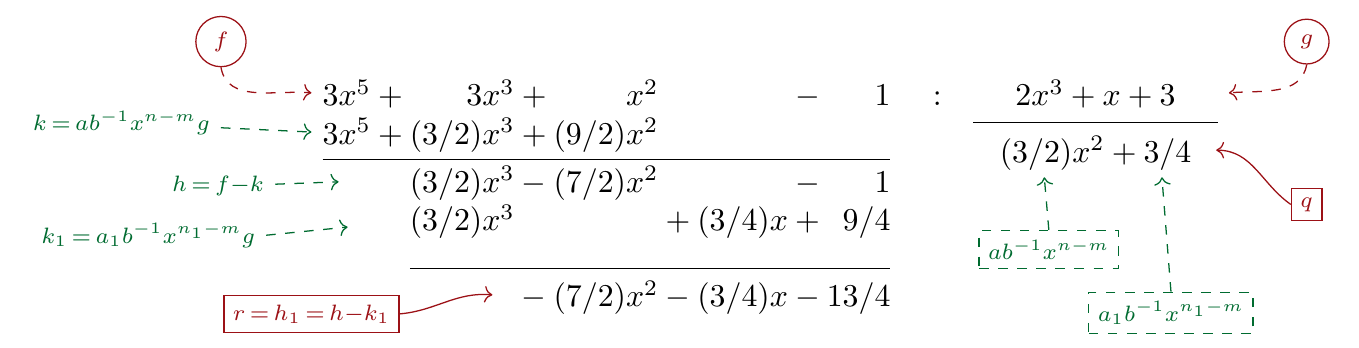
\includegraphics[scale=.4]{res/divisione_polinomiale}
	\end{center}
	
\end{example}

Un caso molto importante è quello dei polinomi a coefficienti in un campo. Infatti, se $A$ è un campo e $0_{A} \neq g \in A[x]$ allora $cd(g)$ è invertibile, come ogni elemento non nullo di $A$. Dunque, in questo caso, l'ipotesi $cd(g) \in \mathcal{U}(A)$ del teorema appena dimostrato può essere sostituita da $g \neq 0_{A}$. Il fatto che ogni polinomio a coefficienti in un campo non sullo sia divisibile ci permette di eseguire l'algoritmo euclideo delle divisioni successive.



\begin{example}
	Per quanto appena detto, se $F$ è un campo, è sempre possibile dividere un polinomio $f \in F[x]$ per un polinomio $g \in F[x] \setminus \{0_{F}\}$. Ad esempio, se $F=\mathbb{Z}_{7}[x]$, vediamo come si divide il polinomio $\overline{2}x^{2}+\overline{3}x+\overline{4}$ per il polinomio $\overline{3}x+\overline{4}$. Un primo modo è quello di effettuare la divisione come se fosse in $\mathbb{Q}[x]$:
	\medskip
	
	\begin{center}
		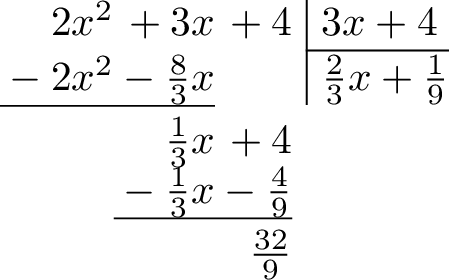
\includegraphics[scale=.25]{res/Divisionez7}
	\end{center}
	\medskip
	
	Quindi:
	\[\overline{2}x^{2}+\overline{3}x+\overline{4} =(\overline{3}x+\overline{4})\Biggl(\frac{\overline{2}}{\overline{3}}x+\frac{\overline{1}}{\overline{9}}\Biggr)+\frac{\overline{32}}{\overline{9}}\]
	Ma cosa sono $\frac{\overline{2}}{\overline{3}}$, $\frac{\overline{1}}{\overline{9}}$ e $\frac{\overline{32}}{\overline{9}}$? In $\mathbb{Z}_{7}$ si ha che $\overline{3}\cdot \overline{5}=\overline{15}=\overline{1}$, quindi $\overline{3}^{-1}=\overline{5}$. Dunque $\frac{\overline{2}}{\overline{3}}=\overline{10}=\overline{3}$. Similmente $\overline{9}^{-1}=\overline{4}$, quindi $\frac{\overline{1}}{\overline{9}}=\overline{4}$ e $\frac{\overline{32}}{\overline{9}}=\overline{32}\cdot \overline{4}=\overline{128}=\overline{1}$. Dunque:
	\[\overline{2}x^{2}+\overline{3}x+\overline{4} =(\overline{3}x+\overline{4})(\overline{3}x+\overline{4})+\overline{2}\]
\end{example}


\subsection{Applicazioni polinomiali}
Sia $f\in A[x]$, dove $A$ è un anello polinomiale. Se $f= \sum_{i=0}^{n} a_{i}x^{i}$ e $c \in A$ si ha:
\begin{displaymath}
	f(c) = \sum_{i=0}^{n} a_{i}c^{i}
\end{displaymath}

\begin{defbox}{Applicazione polinomiale}
	L'applicazione:
	\begin{equation}
		\widetilde{f} : c \in A \mapsto f(c) \in A
	\end{equation}
	che prende il nome di \textbf{applicazione polinomiale} determinata da $f$ in $A$.
\end{defbox}

\begin{osservation}
	A differenza dell'omomorfismo di sostituzione questa applicazione non è, in generale, un omomorfismo. osserviamo che se $f \in A$ allora $f(c)=f$ per ogni $c \in A$, quindi l'applicazione $\widetilde{f}$ è costante. È per questo motivo che gli elementi di $A$ vengono chiamati polinomi costanti.
\end{osservation}


\begin{defbox}{Radice}
	L'elemento $c \in A$ è una \textbf{radice} di $f$ se e solo se $f(c) = 0_{A}$.
\end{defbox}



\begin{lemmabox}\label{lemma:divisori_prodotto_polinomi}
	Siano $A$ un anello commutativo unitario e $f,g \in A[x]$. Allora:
	\begin{enumerate}
		\item se, in $A[x]$, $f$ divide $g$, ogni radice di $f$ in $A$ è radice di $g$.
		\item se $A$ è un dominio di integrità, allora le radici di $fg$ in $A$ sono tutti e soli gli elementi di $A$ che sono radici di $f$ o di $g$.
	\end{enumerate}
	
\end{lemmabox}

\begin{proof}
	\begin{enumerate}
		\item Se $f \divides_{A[x]} g$ esiste $h \in A[x]$ tale che $g=fh$. Allora applicando l'omomorfismo di sostituzione definito da $g$, abbiamo:
		\begin{displaymath}
			g(c) = f(c)h(c) = 0_{A}h(c)=0_{A}
		\end{displaymath}
		dunque $c$ è radice di $g$.
		\item Per la $(1)$, gli elementi di $A$ che sono radici di $f$ o $g$ sono radici anche di $fg$, multiplo di entrambi. Viceversa, se $c$ è radice di $A$ di $fg$, allora:
		\begin{displaymath}
			0_{A} = (fg)(c)=f(c)g(c)
		\end{displaymath}
		Poiché $A[x]$ è un dominio di integrità, questo implica che uno tra $f(c)$ e $g(c)$ è $0_{A}$, quindi $c$ è radice di uno tra $f$ e $g$.
	\end{enumerate}
\end{proof}

\begin{teorbox}[del resto]
	Sia $A$ un anello commutativo unitario e siano $f \in A[x]$ e $c \in A$. Allora $f(c)$ è il resto della divisione di $f$ per $x-c$.
\end{teorbox}

\begin{proof}
	La prima cosa da osservare è che si può certamente effettuare la divisione di $f$ per $x-c$, perché quest'ultimo polinomio è monico, quindi il suo coefficiente direttore è invertibile. Effettuata questa divisione, otteniamo $q,r \in A[x]$ tali che $f=(x-c)q+r$ e si ha $deg r < deg (x-c) =1$. Quest'ultima condizione equivale a dire che $r$ è un polinomio costante. Applichiamo l'omomorfismo di sostituzione:
	\begin{displaymath}
		f(c) = \bigl((x-c)q+r\bigr)(c)= (c-c)q(c)+r(c)=0_{A}q(c)+r=r
	\end{displaymath}
	
	È così provato che $f(c)=r$. 
\end{proof}

\begin{teorbox}[di Ruffini]\label{thm:ruffini}
	Sia $A$ un anello commutativo unitario e siano $f \in A[x]$ e $c \in A$. Allora $c$ è radice di $f$ se e solo se $(x-c)$ divide $f$ in $A[x]$, ovvero se e solo se il resto della divisione di $f$ per $(x-c)$ è zero.
\end{teorbox}

\begin{proof}
	Per il teorema del resto, $c$ è radice di $f$ se e solo se il resto della divisione di $f$ per $x-c$ è zero, cioè se e solo se $x-c$ divide $f$.
\end{proof}

\begin{example}
	Dato il polinomio $f(x)=x^{3}-2x^{2}-5x+10$ abbiamo che $f(2)=0$ e $f(\sqrt{5})$. Per il teorema di Ruffini, abbiamo che $x-2$ e $x-\sqrt{5}$ dividono $f(x)$. Abbiamo infatti:
	\[x^{3}-2x^{2}-5x+10=(x-2)(x^{2}-5=(x-2)(x-\sqrt{5})(x+\sqrt{5})\]
\end{example}


\begin{corolbox}
	Sia $A$ un anello commutativo unitario e siano $f,g \in A[x]$ e $c \in A$. Supponiamo che $f$ e $g$ abbiano in $A[x]$ un massimo comun divisore $d$. Allora le radici comuni a $f$ e $g$ in $A$ sono tutte e sole le radici di $d$ in $A$:
	\begin{equation}
		\{c \in A \; | \; f(c)=0_{A}=g(c)\}=\{c \in A \; | \; d(c)=0_{A}\}
	\end{equation}
\end{corolbox}

\begin{teorbox}[di Ruffini generalizzato]
	Sia $A$ un dominio di integrità unitario e siano $f \in A[x]$, $n \in \mathbb{N}^{*}$ e $c_{1},c_{2}, \ldots, c_{n} \in A$ degli elementi a due a due distinti. Allora si ha che ciascuno degli elementi $c_{i}$ è radice di $f$ se e solo se:
	\begin{displaymath}
		\prod_{i=1}^{n}(x-c_{i}) \divides_{A[x]} f
	\end{displaymath}
\end{teorbox}

\begin{proof}
\begin{itemize}
	\item[$\impliedby$] Ovvio. Se $\prod_{i=1}^{n}(x-c_{i})$ divide $f$ allora ciascuno degli elementi $c_{i}$ è radice di $f$, in quanto $x-c_{i}$ divide $f$.
	
	\item[$\implies$] Si procede per induzione su $n$. Supponiamo che gli elementi $c_{i}$ per ogni $i \in \{1,2,\ldots,n\}$ siano radici di $f$. Se $n=1$ allora $x-c_{1}$ divide $f$ per il teorema di Ruffini. Supponiamo allora $n>1$ e, come ipotesi di induzione, che l'enunciato valga per insiemi di $n-1$ elementi distinti di $A$ ed arbitrari polinomi in $A[x]$.
	
	Poiché $f(c_{n}) = 0_{A}$, per il teorema di Ruffini esiste $q \in A[x]$ tale che $f=(x-c_{n})q$. Sia ora $i$ un intero tale che $1 \leq i < n$. Poiché $c_{i}$ è radice di $f$ e $A$ è un dominio di integrità, segue che $c_{i}$ è radice di uno tra $x-c_{n}$ e $q$ (vedi Lemma \ref{lemma:divisori_prodotto_polinomi}). Dunque ciascuno degli elementi $c_{1},c_{2},\ldots, c_{n-1}$ è radice di $q$. Possiamo allora applicare l'ipotesi di induzione e concludere che: $$\prod_{i=1}^{n-1}(x-c_{i}) \divides_{A[x]} q$$ quindi esiste $h \in A[x]$ tale che:
	\begin{displaymath}
		q = h \prod_{i=1}^{n-1}(x-c_{i})
	\end{displaymath}
	Allora:
	\begin{align*}
		f &= q \cdot (x-c_{n}) \\
		  &= \Bigl( h \cdot \prod_{i=1}^{n-1}(x-c_{i})\Bigr) \cdot (x-c_{n}) \\
		  &= h \prod_{i=1}^{n}(x-c_{i})
	\end{align*}
	Pertanto $\prod_{i=1}^{n}(x-c_{i})$ divide $f$ in $A[x]$ e la dimostrazione è così completa.
\end{itemize}
\end{proof}

Il teorema di Ruffini generalizzato ha due importantissime conseguenze. La prima è una \textbf{limitazione al numero di radici che un polinomio non nullo su un dominio di integrità può avere}.

\begin{teorbox}\label{thm:grado_polinomio}
	Sia $A$ un dominio di integrità unitario e sia $0_{A} \neq f \in A[x]$. Allora il numero delle radici di $f$ in $A$ non supera $deg(f)$.
\end{teorbox}
\begin{proof}
	Se $f$ ha esattamente $n$ radici, siano esse $c_{1},c_{2},\ldots,c_{n}$ allora $f$ è multiplo di $g$:
	\begin{displaymath}
		g \coloneqq \prod_{i=1}^{n}(x-c_{i})
	\end{displaymath}
	Quindi $f = gq$ per un opportuno $q \in A[x]$. Essendo $f\neq 0_{A}$ si ha anche $q \neq 0_{A}$. Ma $deg(g) =n$ e per $g$ e $q$ vale la regola di addizione dei gradi. Quindi $deg(f) = deg(g) + deg (q) = n + deg (q) \geq n$, ovvero $n \leq deg(f)$.
\end{proof}


\begin{osservation}
	Sia per il teorema di Ruffini generalizzato che per il Teorema \ref{thm:grado_polinomio} è \textbf{essenziale l’ipotesi che l'anello sia un dominio di integrità}. Sia $f=\overline{2}x \in \mathbb{Z}_{6}[x]$. Sia $\overline{0}$ che $\overline{3}$ sono radici del polinomio, quindi $f$ ha più radici di quanto sia il suo grado, che è 1. Inoltre, come imposto dal teorema di Ruffini sia $x = x - \overline{0}$ che $x- \overline{3}$ dividono $f$. Infatti:
	\begin{align*}
		f = x \cdot \overline{2} = (x- \overline{3}) \cdot \overline{2}
	\end{align*}
Ma osserviamo che $x(x-\overline{3})$ non divide $f$, quindi la conclusione di Ruffini generalizzato \emph{non vale} per $f$.
\end{osservation}

L’altra conseguenza del teorema di Ruffini generalizzato riguarda le applicazioni polinomiali e ci dice che, \textbf{nel caso dei domini di integrità infiniti, ogni polinomio è identificato univocamente dalla sua applicazione polinomiale}.

\begin{propbox}
	Principio di identità dei polinomi
	Sia $A$ un dominio di integrità infinito. Allora, per ogni $f,g \in A[x]$ si ha:
	\begin{displaymath}
		\widetilde{f} = \widetilde{g} \iff f=g
	\end{displaymath}
\end{propbox}

\begin{proof}
	Ovviamente $\widetilde{f} = \widetilde{g}$ se $f=g$. Supponiamo, viceversa, $\widetilde{f} = \widetilde{g}$. Allora $f(c)=g(c)$ per ogni $c \in A$. Sia $h = f-g$. Allora, per ogni $c \in A$ abbiamo $h(c) = (f-g)(c)=f(c)-g(c)=0_{A}$, vale a dire: ogni elemento di $A$ è radice di $h$. Dunque $h$ ha un numero infinito di radici. Ma il Corollario precedente assicura che, se $h \neq 0_{A}$, allora il numero delle radici di $h$ non supera $deg(h)$, quindi è finito. Di conseguenza deve essere $h=0_{A}$, ovvero $f=g$.
\end{proof}


È a causa del principio di identità dei polinomi che in alcuni casi vengono identificati i polinomi con le applicazioni polinomiali. Ad esempio, nei corsi di analisi matematica si definiscono i polinomi come particolari funzioni da $\mathbb{R}$ a $\mathbb{R}$, quelle che per noi sono le applicazioni polinomiali definite dai polinomi in $\mathbb{R}[x]$. Questo è lecito perché, essendo $\mathbb{R}$ un campo (quindi un dominio di integrità) infinito, il principio di identità dei polinomi assicura che i polinomi in $\mathbb{R}[x]$ corrispondono esattamente alle loro applicazioni polinomiali (in corsi di analisi più avanzati i polinomi sono definiti con riferimento al campo complesso, anziché a quello reale; il discorso è analogo: anche per il campo complesso vale il principio di identità dei polinomi). D’altra parte, \emph{non è lecito identificare polinomi ed applicazioni polinomiali in contesti in cui non valga il principio di identità dei polinomi}, cioè quando l’anello $A$ considerato sia finito oppure non sia integro.


Nel caso degli anelli finiti è certo che il principio di identità dei polinomi non può valere. Infatti, se $A$ è un anello commutativo unitario finito, il numero delle applicazioni da $A$ ad $A$, e quindi il numero delle applicazioni polinomiali in $A$, è finito, mentre $A[x]$ è comunque infinito. Dunque, in questo caso, è impossibile che ci sia una corrispondenza biunivoca tra polinomi e applicazioni polinomiali (ciò che il principio di identità dei polinomi afferma è che, se $A$ è un dominio di integrità infinito, l’applicazione $f \in A[x] \mapsto  \widetilde{f} \in Map(A, A)$ è iniettiva; ciò è impossibile nel caso che stiamo considerando ora, in cui il dominio $A[x]$ è infinito ma il codominio $Map(A, A)$ è finito).


\begin{example}
	Consideriamo il polinomio $f= x^{3}-x \in \mathbb{Z}_{3}[x]$. Si ha:
	\begin{align*}
		\overline{f}([0]_{3}) &= \overline{0}^{3}-\overline{0} = \overline{0}\\
		\overline{f}([1]_{3}) &= \overline{1}^{3} - \overline{1} = \overline{0}\\
		\overline{f}([2]_{3}) &= \overline{2}^{3} -\overline{2} = \overline{8}-\overline{2}=\overline{6}=\overline{0}
	\end{align*}
	Quindi $\overline{f} = \overline{0}$ ma $f \neq \overline{0}$.
\end{example}

\subsection{Fattorizzazione}

Ricordiamo che un monoide commutativo cancellativo (cioè ad elementi tutti cancellabili) si dice \textbf{fattoriale} se e
solo se ogni suo elemento non invertibile è prodotto di elementi irriducibili e tali decomposizioni in irriducibili
sono essenzialmente uniche.


\begin{teorbox}
	Se $A$ è un anello fattoriale allora $A[x]$ è fattoriale.
\end{teorbox}


Sono certamente fattoriali i campi ed è fattoriale, per il Teorema Fondamentale dell’Aritmetica, l’anello $\mathbb{Z}$ degli interi. Quindi è fattoriale $\mathbb{Z}[x]$ e, per ogni campo $K$, anche $K[x]$. Dunque, sia per i polinomi a coefficienti in $\mathbb{Z}$ che per quelli a coefficienti in un campo vale un teorema di fattorizzazione essenzialmente unica in prodotto di polinomi irriducibili: \textit{ogni polinomio non invertibile e non nullo è prodotto di polinomi irriducibili e tale fattorizzazione è unica a meno dell’ordine dei fattori e della sostituzione di alcuni fattori con polinomi associati.}



Se $K$ è un campo, si ha:
\begin{displaymath}
	\mathcal{U}(K[x]) = \mathcal{U}(K) = K \setminus \{0_{K}\}
\end{displaymath}
Quindi l'insieme di tutti i polinomi associati ad un $f \in K[x] \setminus \{0_{K}\}$ è:
\begin{displaymath}
	\{uf \; | \; u \in K \setminus \{0_{K}\} \}
\end{displaymath}
Se $a = cd(f)$, si ha $cd(uf)=ua$ per ogni $u \in K \setminus \{0_{K}\}$. Allora, qualunque sia $k \in K \setminus \{0_{K}\}$, il polinomio $f$ ha esattamente un associato con coefficiente direttore $k$, precisamente $(ka^{-1})f$. Infatti, per ogni $u \in K \setminus \{0_{K}\}$ abbiamo che $cd(uf) =ua = k$ se, e solo se, $c = ka^{-1}$.

\begin{propbox}
	Sia $K$ un campo. In ogni classe di elementi associati di polinomi non nulli in $K[x]$ esiste uno ed un solo polinomio monico che prende il nome di \textbf{rappresentante monico}.
\end{propbox}


\begin{example}
	In $\mathbb{Q}[x]$ il polinomio monico associato a $f = 3x^{2}+x-6$ è:
	\begin{displaymath}
		(\frac{1}{3})f = x^{2}+ \frac{1}{3}x -2
	\end{displaymath}
	ma anche:
	\begin{displaymath}
		-6x^{2}-2x+12
	\end{displaymath}
	e infiniti altri polinomi della forma $uf$, dove $0 \neq u \in \mathbb{Q}$.
\end{example}

\begin{propbox}
	Sia $K$ un campo. Allora ogni polinomio non nullo in $K[x]$ è prodotto di un elemento di $K$ e di polinomi monici irriducibili in $K[x]$. Tale fattorizzazione è unica a meno dell’ordine dei fattori.
\end{propbox}

\begin{proof}
	L'unicità della fattorizzazione segue dal fatto che $K[x]$ è fattoriale e dal fatto che ogni classe di polinomi associati non nullo contiene un solo rappresentante monico. L'esistenza della decomposizione è ovvia nel caso dei polinomi costanti, va provata per polinomi non costanti. Sia, allora $f \in K[x] \setminus K$. Sia $f=p_{1}p_{2}\cdot \ldots \cdot p_{n}$ una fattorizzazione di $f$ in prodotto di polinomi irriducibili. Per ogni $i \in \{1,2,\ldots, n\}$ sia $a_{i} = cd (p_{i})$; allora $p_{i}=a_{i}q_{i}$, dove $q_{i}=a_{i}^{-1}p_{i}$ è associato a $p_{i}$ (quindi è irriducibile) ed è monico. Posto $a= a_{1}a_{2}\cdot \ldots \cdot a_{n}$ abbiamo $f=aq_{1}q_{2}\ldots q_{n}$. Questa è la decomposizione cercata.
\end{proof}

\begin{osservation}
	Nell’ipotesi che $A$ sia fattoriale, una delle conseguenze del fatto che $A[x]$ è fattoriale è che, nota una fattorizzazione in prodotto di irriducibili di un polinomio $f$, è facile determinare l’insieme dei divisori di $f$. Posto infatti $f=p_{1}^{\lambda_{1}} \cdot p_{2}^{\lambda_{2}} \cdot \ldots \cdot p_{n}^{\lambda_{n}}$, dove i $p_{i}$ sono polinomi irriducibili e per ogni $i \neq j$ $p_{i}$ e $p_{j}$ non sono associati, l'\textbf{insieme dei divisori} di $f$ è dato da tutti i polinomi della forma:
	\[
	p_{1}^{\sigma_{1}} \cdot p_{2}^{\sigma_{2}} \cdot \ldots \cdot p_{n}^{\sigma_{n}}
	\]
	ed i loro associati, dove, per ogni $i$, $\sigma_{i} \in \mathbb{N}$ e $\sigma_{i} \leq \lambda_{i}$.
\end{osservation}

Quindi, ogni polinomio non nullo di grado diverso da zero a coefficienti su un campo $K$ (ciò vale a dire: ogni elemento non zero e non invertibile di $K[x]$) si fattorizza in modo essenzialmente unico come prodotto di polinomi irriducibili. Poiché ogni classe di polinomi irriducibili associati contiene uno ed un solo polinomio monico, possiamo concludere che, se $K$ è un campo, allora ogni polinomio $f \in K[x]\setminus K$ si scrive in modo unico (a meno dell'ordine dei fattori) come:
\[
f= a_{n} f_{1} f_{2} \ldots f_{k}
\]
dove $a_{n}$ è il coefficiente direttore di $f$ e $f_{1},f_{2}, \ldots, f_{k}$ sono polinomi monici irriducibili in $K[x]$. Ci vogliamo ora occupare di descrivere, per quanto possibile, la proprietà di essere o meno \textbf{irriducibile} per un polinomio a coefficienti in un campo. Vedremo in che modo questo proprietà è collegata alla presenza di radici.


\begin{example}
	In $\mathbb{Q}[x]$, $x^{2}-1$ ammette la fattorizzazione:
	\begin{displaymath}
		x^{2}-1 = (x-1)(x+1)
	\end{displaymath}
	In realtà $x^{2}-1$ ammette altre decomposizioni, come $(\frac{1}{2}x-\frac{1}{2})\cdot(2x+2)$. Tuttavia $x+1$ e $2x+2$ sono associati, differiscono cioè per un fattore invertibile. Allo stesso modo $x-1$ e $\frac{1}{2}x-\frac{1}{2}$ sono associati. Quindi sostanzialmente le due decomposizioni sono la stessa.
\end{example}

\begin{propbox}[Criterio di irriducibilità]
	Siano $K$ un campo e $f \in K[x]$. Se $n= deg(f)$ allora $f$ è irriducibile in $K[x]$ se e solo se $n>0$ e vale una delle due proprietà equivalenti:
	\begin{enumerate}
		\item non esistono $g,h \in K[x]$ tali che $f=gh$ e sia $g$ che $h$ abbiano grado minore di $n$;
		\item non esistono $g,h \in K[x]$ tali che $f=gh$ e sia $g$ che $h$ abbiano grado maggiore di $0$.
	\end{enumerate}
\end{propbox}

\begin{proof}
Ricordiamo che $f$ è irriducibile se e solo se, in $K[x]$, non è invertibile e non ha divisori se non
	quelli banali. Possiamo subito osservare che i polinomi costanti non sono irriducibili. Infatti i polinomi costanti non nulli sono invertibili, mentre il polinomio nullo ha tutti gli elementi di $K[x] \setminus K$ come divisori non banali. Abbiamo così che l’asserto è corretto nel caso in cui $f$ sia costante: $f$ non è irriducibile e non è vero che $n = deg(f) > 0$, quindi la condizione all’enunciato non è soddisfatta. 
	
	Possiamo allora assumere $f \notin K$, cioè: $n > 0$. Supponiamo dunque $n > 0$. osserviamo che, se $g,h \in K[x]$ e $f=gh$, per la regola di addizione dei gradi (che vale perché $K$ è un campo) si ha:
	$$n=deg(f)=deg(g)+deg(h)$$
	Quindi $deg(g)<n$ e $deg(h)<n$ che è equivalente alla condizione $(deg(g)>0 \land deg(h)>0)$, vale a dire che la (1) e la (2) sono equivalenti. 
	
	Se $f$  è irriducibile, scelti comunque $g,h \in K[x]$ tali che $f=gh$, allora $g$ è un divisore di $f$, quindi un divisore banale perché $f$ è irriducibile. Allora o $g$ è invertibile, nel qual caso $g \in K \setminus \{0_{K}\}$ e $deg(g)=0$, oppure $g$ è associato ad $f$, nel qual caso $deg(g)=deg(f)=n$. Ciò mostra che, se $f$ è irriducibile, sono verificate (1) e (2). 
	
	Se invece $f$ non è irriducibile, $f$ ha un divisore non banale $g$, allora $g \neq 0_{K}$ e $g$ non è invertibile, quindi $deg(g)>0$ ed esiste $h \in K[x]$ tale che $f=gh$. Ovviamente $h \neq 0_{K}$ e $h$ non è invertibile perché $g$ non è associato ad $f$, quindi abbiamo anche $deg(h)>0$. In questo caso, dunque, non vale (2) e quindi neanche (1).
\end{proof}


\begin{osservation}
	Un’ovvia conseguenza di questa caratterizzazione è che \textit{i polinomi di primo grado a coefficienti in un campo $K$ sono certamente irriducibili in $K[x]$}, dal momento che i prodotti tra polinomi di grado minore di $1$ sono certamente costanti.
\end{osservation}



\begin{propbox}
	Sia $K$ un campo e sia $f \in K[x]$. Allora $f$ ha radici in $K$ se e solo se ha almeno un divisore di primo grado in $K[x]$.
\end{propbox}


\begin{propbox}
	Sia $A$ un dominio di integrità unitario e sia $f \in A[x]$. Se $deg(f) > 1$ e $f$ ha radici in $A$, allora $f$ è riducibile in $A[x]$.
\end{propbox}

\begin{propbox}
	Siano $K$ un campo e $f$ un polinomio in $K[x]$ di grado 2 o 3. Allora $f$ è irriducibile in $K[x]$ se e solo se è privo di radici in $K$.
\end{propbox}

Possiamo schematizzare come segue le informazioni ottenute sulle proprietà di un polinomio a coefficienti in un campo di essere o meno irriducibile ed di avere o meno radici. Se $K$ è un campo e $0_{K} \neq f \in K[x]$, posto $deg(f) = n$ si ha:
\begin{center}
	\begin{tblr}{hlines,cells={mode=math},colspec={|ccl|}}
		n = 0 & \implies & \text{$f$ è invertibile e privo di radici} \\
		n = 1 & \implies & \text{$f$ è irriducibile ed ha una radice}\\
		n \in \{2,3\} & \implies & \text{$f$ irriducibile} \iff \text{$f$ non ha radici} \\
		n>3 & \implies &  \text{$f$ irriducibile} \implies \text{$f$ non ha radici}
	\end{tblr}
	\captionof{table}{Irriducibilità di un polinomio in un campo}\label{tab:irridicibili}
\end{center}

\subsection{Metodi ed esempi di fattorizzazione per polinomi su un campo}
Supponiamo di voler fattorizzare un polinomio (in un fissato anello di polinomi) in prodotto di polinomi irriducibili. Per farlo abbiamo bisogno:
\begin{itemize}
	\item di saper trovare divisori non banali del polinomio dato, se ne esistono;
	\item di saper riconoscere quali tra questi divisori sono irriducibili.
\end{itemize}

Limitiamoci al caso dei polinomi su un campo. Usando la tabella nella sezione precedente, sappiamo, in linea di
massima, rispondere al secondo punto nel caso di divisori di grado minore di quattro. I polinomi di grado uno
sono sempre irriducibili, quelli di grado due o tre lo sono se e solo se sono privi di radici. In due casi notevoli
queste informazioni sono addirittura più di quanto non sia necessario. Infatti valgono questi teoremi (che non
dimostriamo) per polinomi in $\mathbb{R}[x]$.

\begin{teorbox}
	Ogni polinomio irriducibile in $\mathbb{R}[x]$ ha grado minore di 3.
\end{teorbox}


Dunque, i polinomi irriducibili in $\mathbb{R}[x]$ sono precisamente quelli di grado 1 e quelli di grado 2 privi di radici. Come è noto dalle scuole superiori, un polinomio $ax^{2} + bx + c \in \mathbb{R}[x]$ di grado 2 ha radici in $\mathbb{R}$ se e solo se $b^{2}- 4ac \geq 0 $.

\begin{teorbox}[di Bolzano]
	Ogni polinomio di grado dispari in $\mathbb{R}[x]$ ha qualche radice in $\mathbb{R}$.
\end{teorbox}

La situazione è molto più complessa (ed interessante) nel caso di polinomi in $\mathbb{Q}[x]$. Lo studio dei polinomi in $\mathbb{Q}[x]$ si può ridurre al caso dei polinomi a coefficienti interi. Ricordiamo che $\mathbb{Z}[x]$ è un dominio di integrità, così come $\mathbb{Q}[x]$, ma gli unici elementi invertibili di $\mathbb{Z}[x]$ sono $\pm 1$, cioè gli stessi di $\mathbb{Z}$. Inoltre i polinomi di $\mathbb{Z}[x]$ che dividono un intero $a_{0} \neq 0$ devono avere grado zero, cioè solo a loro volta interi. Dunque:
\begin{itemize}
	\item $a_{0}$ ha gli stessi divisori in $\mathbb{Z}[x]$ e $\mathbb{Z}$;
	\item in particolare $a_{0}$ è invertibile in $\mathbb{Z}[x]$ se e solo se è invertibile in $\mathbb{Z}$, cioè se e solo se è $\pm 1$;
	\item per $a_{0} \neq \pm 1$, $a_{0}$ ha le stesse decomposizioni in prodotto di fattori irriducibili in $\mathbb{Z}[x]$ e in $\mathbb{Z}$.
\end{itemize}

\begin{defbox}{Polinomio primitivo}
	Sia $f(x)$ un polinomio a coefficienti interi. Si dice che $f(x)$ è primitivo se il massimo comun divisore dei suoi coefficienti è 1.	Un polinomio monico intero è primitivo.
\end{defbox}

\begin{teorbox}
	Ogni polinomio $f \in \mathbb{Q}[x]$ è associato, in $\mathbb{Q}[x]$ ad un polinomio $\overline{f} \in \mathbb{Z}[x]$.
\end{teorbox}

\begin{example}
	Ad ogni polinomio $b(x) \in \mathbb{Q}[x]$ è associato un polinomio primitivo $a(x) \in \mathbb{Z}[x]$ ottenuto moltiplicando $b(x)$ per il minimo comune multiplo dei suoi coefficienti e successivamente dividendo il polinomio così ottenuto per il massimo comun divisore dei coefficienti. Ad esempio, il polinomio $f(x) = \frac{1}{2}x^{2}+\frac{3}{4}x+\frac{1}{3}$ è associato al polinomio primitivo $g(x) = \frac{12}{2}x^{2}+\frac{12 \cdot 3}{4}x+\frac{12}{3}=6x^{2}+9x+4$.
\end{example}

Ora, polinomi tra loro associati hanno esattamente le stesse proprietà rispetto alla fattorizzazione.

\begin{propbox}[Criterio di Eisenstein]
	Sia $f= a_{0}+a_{1}x+a_{2}x^{2}+ \ldots + a_{n}x^{n} \in \mathbb{Z}[x]$. Se esiste un primo $p \in \mathbb{P}$ tale che:
	\begin{enumerate}
		\item $p$ divide $a_{0},a_{1}, \ldots, a_{n-1}$
		\item $p$ non divide $a_{n}$
		\item $p^{2}$ non divide $a_{0}$
	\end{enumerate}
	allora $f$ è irriducibile in $\mathbb{Q}[x]$.
\end{propbox}

\begin{osservation}
	Per ogni intero positivo $n$ e per ogni primo $p$, il polinomio $x^{n} - p$ è irriducibile in $\mathbb{Q}[x]$ e dunque in $\mathbb{Q}[x]$ ci sono polinomi irriducibili di ogni grado.
\end{osservation}


\begin{teorbox}[delle radici razionali]\label{prop:car_radici_Q}
	Sia $f=a_{n}x^{n}+a_{n-1}x^{n-1}+\ldots+a_{2}x^{2}+ a_{1}x +a_{0} \in \mathbb{Z}[x]$, un polinomio a coefficienti interi con $a_{n} \neq 0$. Allora ogni soluzione razionale di $f$ (ogni radice in $\mathbb{Q}$) si scrive come frazione $u/v$, dove $u$ e $v$ sono interi coprimi e $u$ è un divisore del termine noto $a_{0}$ e $v$ è un divisore del coefficiente direttore $a_{n}$.
\end{teorbox}

\begin{proof}
	Ogni numero razionale si può scrivere come frazione ridotta, quindi nella forma $u/v$, dove $u$ e $v$ sono interi coprimi e $v \neq 0$. Se una tale frazione $u/v$ è radice di $f$ allora:
	\begin{displaymath}
		0 = a_{0}v^{n} + a_{1}uv^{n-1} + a_{2}u^{2}v^{n-2}+ \ldots + a_{n-2}u^{n-2}v^{2}+ a_{n-1}u^{n-1}v + a_{n}u^{n}=0
	\end{displaymath}
	Ora, escluso (per il momento) il primo, tutti gli addendi a primo membro sono multipli di $u$. Poiché la loro somma vale 0, il primo addendo $a_{0}v^{n}$ è l'opposto della somma dei rimanenti. Quindi anch'esso è un multiplo di $u$. Dunque $u$ divide $a_{0}v^{n}$. Ma $u$ è coprimo con $v$, quindi con $v^{n}$, dunque $u$ divide $a_{0}$. In modo analogo $v$ divide $a_{n}$.
\end{proof} 

\begin{osservation}
	Ogni polinomio in $\mathbb{Q}[x]$ è associato (in $\mathbb{Q}[x]$) ad un polinomio in $\mathbb{Z}[x]$, che avrà le stesse radici razionali. 
\end{osservation}

Quindi, per cercare le radici razionali di un polinomio in $\mathbb{Q}[x]$ possiamo cercare le radici razionali del suo associato in $\mathbb{Z}[x]$. Questo è un vantaggio perché, come abbiamo visto, la ricerca delle radici razionali di un polinomio in $\mathbb{Z}[x]$ è semplificata dal criterio di Eisenstein e dalla proposizione \ref{prop:car_radici_Q}.
 
Volendo ricercare le radici razionali di un polinomio $f \in \mathbb{Q}[x]$ possiamo quindi procedere come segue:
\begin{enumerate}
	\item Sostituiamo il polinomio con un suo associato a coefficienti interi;
	\item Si considera il coefficiente direttore $a_{n}$ ed il termine noto $a_{0}$ del polinomio.
	\item Le radici razionali del polinomio sono le frazioni della forma $u/v$ con $u$ e $v$ interi coprimi tali che $u$ divida $a_{0}$ e $v$ divida $a_{n}$.
\end{enumerate}

È chiaro che (escluso il caso, banalmente semplificabile, in cui $a_{0}=0$) esiste solo un numero finito di tali frazioni, possiamo allora verificare per ciascuna di esse se è o meno radice del polinomio.


\begin{example}
	Consideriamo il polinomio $f=x^{4}-4x^{2}+(3/2)x+3 \in \mathbb{Q}[x]$. Un suo associato a coefficienti interi è: $$2f=2x^{4}-8x^{2}+3x+6$$
	con coefficiente direttore $2$ e termine noto $6$. Le frazioni della forma $\frac{u}{v}$ con $u$ e $v$ interi coprimi tali che $u$ divida $6$ e $v$ divida $2$ sono: $1=\frac{1}{1}$, $\frac{1}{2}$, $2$, $3$, $\frac{3}{2}$, $6$ e i loro opposti. 
	
	Per cercare tutte le radici razionali di $f$ non dobbiamo fare altro che \textit{controllare quali di questi dodici numeri sono radici di $f$ in $\mathbb{Q}[x]$}. Nel nostro caso la verifica diretta mostra che solo $-2$ è radice. Concludiamo che $-2$ è l'unica radice in $\mathbb{Q}[x]$.
	
	Possiamo proseguire lo studio di questo polinomio cercando di fattorizzarlo in prodotto di irriducibili. Usiamo il Teorema di Ruffini; dividendo $f$ per $x+2$ (cioè $(x-(-2))$) otteniamo: $$f=(x+2)(x^{3}-2x^{2}+3/2)$$
	
	Il secondo fattore $f_{1}$ di questo prodotto è associato a $2f_{1}=2x^{3}-4x^{2}+3$. Sfruttando la proposizione \ref{prop:car_radici_Q} concluderemmo che le radici di $f_{1}$ sono da cercare tra le frazioni ridotte della forma $u/v$ dove $u,v \in \mathbb{Z}$, $u$ divide 3 e $v$ divide 2. 
	
	In realtà non è necessario esaminare tutte queste frazioni perché ogni radice di $f_{1}$ è anche radice di $f$ e di tutte queste frazioni, tranne -2, sappiamo che non sono radici di $f$, quindi nemmeno di $f_{1}$. Dobbiamo esaminare solo $-2$, si ha: $$f_{1}(-2)=(-2)^{3}-2(-2)^{2}+3/2\neq 0$$quindi $-2$ non è radice di $f_{1}$. Pertanto $f_{1}$ non ha radici in $\mathbb{Q}$; poiché $deg(f)=3$ concludiamo che $f_{1}$ è irriducibile in $\mathbb{Q}[x]$. 	Dunque una fattorizzazione (l'unica a meno dell'ordine) di $f$ in prodotto di irriducibili monici in $\mathbb{Q}[x]$ è: \[f=(x+2)(x^{3}-2x^{2}+3/2)\]
\end{example}
\marker{yellow!50}{yellow!20!black}{Quando la cardinalità del campo	finito $F$ è piccola il metodo più efficace per la ricerca delle radici di un polinomio $f \in F[x]$ è spesso la verifica diretta eseguita per ogni elemento, vale a dire il calcolo di $f(c)$ per ogni elemento $c$ del campo.}
\newpage
\section{Esercizi svolti}
\subsection{Aritmetica e congruenze}
\begin{exsbox}
	Determinare il più grande numero naturale $k<100$ per cui ammette soluzione l'equazione diofantea $8x+12y=k$ e risolverla.
\end{exsbox}

\paragraph{Svolgimento.} Sappiamo che una equazione diofantea è risolubile se il massimo comune divisore tra i due coefficienti delle incognite divide il termine noto.

In questo caso $MCD(8,12)=4$ e il più grande numero naturale, minore di 100 e multiplo di 4 è 96. L'equazione diofantea diventa quindi:
\[8x+12y=96\]
Per il Teorema di Bezout possiamo esprimere 4 come combinazione lineare di 8 e 12 e abbiamo:
\[4 = 8 \cdot -1 + 12 \cdot 1\]
Quindi la coppia $(-1,1)$ è soluzione dell'equazione diofantea $8x+12y=4$. Essendo $96= 4 \cdot 24$, moltiplicando la coppia $(-1,1)$ per 24 si ottiene la coppia $(-24,24)$ che è la soluzione ricercata. \hfill \blacksquare

\begin{exsbox}
	Determinare l'insieme $X=\{n \in \mathbb{Z} / 16(1-n) \equiv_{36} 12n+a\}$ per almeno un $a \in \{6,7,8,9\}$.
\end{exsbox}
\paragraph*{Svolgimento.} Per come è stato definito l'insieme $X$ possiamo dare una descrizione di tale insieme più estesa, ovvero:
\begin{align*}
	X = \{n \in \mathbb{Z} / 16(1-n) \equiv_{36} 12n+ 6 \} \cup \{n \in \mathbb{Z} / 16(1-n) \equiv_{36} 12n+ 7\} \\
	\cup \{n \in \mathbb{Z} / 16(1-n) \equiv_{36} 12n+8\} \\
	\cup \{n \in \mathbb{Z} / 16(1-n) \equiv_{36} 12n+9\}
\end{align*}
L'insieme $X$ è costituito quindi dagli interi che sono soluzione delle quattro equazioni congruenziali. L'equazione congruenziale generica è:
\begin{equation}\label{eq:esercizio_congruenze1}
	16(1-n) \equiv_{36} 12n+a
\end{equation}
con $a \in \{6,7,8,9\}$. Risolvere l'equazione \ref{eq:esercizio_congruenze1} significa ricercare i numeri interi tali che:
\begin{align*}
	36 \divides 16(1-n) - (12n+a) &\iff \exists k \in \mathbb{Z} \bigl(16(1-n) - (12n+a) = k \cdot 36 \bigr) \\
	&\iff \exists k \in \mathbb{Z} \bigl(16-16n - 12n -a = k \cdot 36 \bigr) \\
	&\iff \exists k \in \mathbb{Z} \bigl(16-28n -a = k \cdot 36 \bigr) & \text{\textcolor{gray}{Svolgendo l'espressione algebrica}}\\
	&\iff \exists k \in \mathbb{Z} \bigl((16-a) -28n = k \cdot 36\bigr) \\
\end{align*}
La ricerca delle soluzioni si riduce quindi alla risoluzione delle quattro equazioni congruenziali:
\begin{eqnarray}
	28n \equiv_{36} 16-6  \iff 28n \equiv_{36} 10 \\
	28n \equiv_{36} 16-7  \iff 28n \equiv_{36} 9\\
	28n \equiv_{36} 16-8  \iff 28n \equiv_{36} 8 \label{eq:esercizio_congruenze_risolubile}\\
	28n \equiv_{36} 16-9 \iff 28n \equiv_{36} 7
\end{eqnarray}
Procediamo quindi con la risoluzione della prima equazione. Il massimo comun divisore tra 28 e 36 è 4 e $4 \ndivides 10$, quindi la prima soluzione non ammette soluzioni per $a=6$. Analogamente per $a=7$ e $a=9$. Procediamo con l'equazione \ref{eq:esercizio_congruenze_risolubile} in quanto $(28,36) \divides 8$. Dividendo l'equazione per il massimo comune divisore si ottiene l'equazione congruenziale equivalente:
\begin{displaymath}
	7n \equiv_{9} 2
\end{displaymath}
Infatti sappiamo che le soluzioni di $28n \equiv_{36} 8$ sono tutte e sole quelle di $\frac{28}{4}n \equiv_{\frac{36}{4}} \frac{8}{4}$, ovvero $7n \equiv_{9} 2$, in quanto $4$ risulta essere un divisore comune di $28$, $36$ e $8$. Il vantaggio di tale semplificazione è dato dal fatto che $[7]_{9}$ è invertibile in $\mathbb{Z}_{9}$ in quanto $(7,9)=1$, ovvero 7 e 9 sono coprimi. Sfruttando il \hyperlink{thm:bezout}{Teorema di Bezout} possiamo quindi trovare un inverso di 7 in $\mathbb{Z}_{9}$. Esistono infatti due interi $u,v$ tali che: $1 = 7u+9v$. Chiaramente $1 = 28-27 =7 \cdot 4 - 9 \cdot 3$ e quindi $7 \cdot 4 -1 = 9 \cdot (-3)$. Abbiamo così dimostrato che la coppia $(4,-3)$ è una soluzione dell'equazione diofantea $1=7u+9v$. Moltiplicando per 2 si ottiene $2=7 \cdot 8  + 9 \cdot (-6) =56-54$ e si ha: $7 \cdot 8 -2 = 9 \cdot (-6)$, ovvero $9 \divides 7 \cdot 8 - 2$, cioè  $7 \cdot 8 \equiv_{9} 2$. Quindi $n=8$ è una soluzione dell'equazione $7n \equiv_{9} 2$, che è equivalente a dire che la classe di resto $[8]_{9}$ è una soluzione di tale equazione.

Concludiamo quindi dicendo che $X = \{n \in \mathbb{Z} / \exists k \in \mathbb{Z} (n = 9k+ 8)\}$. \hfill \blacksquare

\begin{exsbox}
	Verificare che l'insieme $\mathbb{Z}_{3}$ munito dell'operazione di addizione è un gruppo commutativo.
\end{exsbox}

\paragraph{Svolgimento.} Per dimostrare che $(\mathbb{Z}_{3},+)$ sia un gruppo commutativo dobbiamo dimostra che $(\mathbb{Z}_{3},+)$ risulta essere un monoide commutativo e che per ogni elemento di tale struttura esista l'opposto.
Come sappiamo $(\mathbb{Z}_{3},+)$ risulta essere una struttura algebrica definita dall'operazione indotta dalla relazione $\equiv_{3}$ nella struttura $(\mathbb{Z},+)$. Dai risultati\footnote{Vedi \ref{sez:congruenze}} dimostrati per le congruenze sappiamo che $+_{\equiv_{3}}$ conserva l'associatività e la commutatività. Quindi $(\mathbb{Z}_{3},+)$ è un semigruppo commutativo. Inoltre, preso $0 \in \mathbb{Z}$ elemento neutro in $(\mathbb{Z},+)$ si ha che $[0]_{3}$ risulta essere l'elemento neutro in $(\mathbb{Z}_{3},+)$ che risulta quindi un monoide commutativo. Se $-a \in \mathbb{Z}$ è l'opposto di $a \in \mathbb{Z}$ secondo l'operazione $+$ allora $[-a]_{3} = [a]_{3}$ è l'opposto dell'elemento $[a]_{3} \in \mathbb{Z}_{3}$ e $(\mathbb{Z}_{3},+)$ è quindi un gruppo abeliano. \hfill \blacksquare

\begin{exsbox}
	Si determinino le soluzioni della congruenza: $324x \equiv_{508} 127$.
\end{exsbox}
\paragraph*{Svolgimento.} L'equazione $324x \equiv_{508} 127$ non ha soluzioni. Infatti, calcolato  $MCD(324,508)=2$ si osserva che $2 \ndivides 127$. \hfill \blacksquare

\begin{exsbox}
	Si determinino le soluzioni della congruenza $3x \equiv_{8} 5$.
\end{exsbox}

\paragraph*{Svolgimento.}
Sappiamo che la congruenza ammette soluzioni intere poiché il massimo comun divisore tra 3 ed 8 è 1 che divide 5. Per determinare una soluzione scrivo 1 come combinazione linare di tre ed otto, risolvo cioè l'equazione diofantea:
\begin{displaymath}
	3x+8y=1
\end{displaymath}
Chiaramente, dalla divisione euclidea abbiamo:
\begin{displaymath}
	\left \lbrace
	\begin{array}{l}
		8 = 3 \cdot 2 + 2 \\
		3 = 2 \cdot 1 + 1 \\
	\end{array}
	\right .
	\implies
	\left\lbrace
	\begin{array}{l}
		2 = 8 - 3 \cdot 2\\
		1 = 3 - 2
	\end{array}
	\right .
\end{displaymath}
Quindi:
\begin{align*}
	1	&=  3 -  2  \\
	&= 3 -( 8-3 \cdot 2)\\
	&= 3 + 3 \cdot 2 - 8 \\
	&= 3 \cdot 3 -8 \\
	&= 3 \cdot 3 + (-1) \cdot 8
\end{align*}
Moltiplicando per 5 abbiamo che:
\begin{displaymath}
	5 = 15 \cdot 3 + (-5) \cdot 8
\end{displaymath}
e quindi $3 \cdot 15 \equiv_{8} 5$, ovvero ogni intero congruo a 15 (e cioè congruo a 7) modulo 8 è soluzione della congruenza. Dalla teoria sappiamo poi che l'insieme di tutte le soluzioni è costituito dagli interi congrui (modulo 8) a:
\begin{displaymath}
	x_{0} + t \cdot \frac{8}{(3,8)} =7+8t
\end{displaymath}
al variare di $0 \leq t < (3,8)=1$. Pertanto solo per $t=0$ si hanno soluzioni e queste sono dunque tutti e soli gli interi congrui a 7 modulo 8, ovvero la classe di resto $[7]_{8}$. \hfill \blacksquare
\begin{exsbox}
	Trovare le soluzioni dell'equazione congruenziale $87x \equiv_{12} 27$.
\end{exsbox}
\paragraph{Svolgimento.} Applicando l'algoritmo euclideo delle divisioni successive abbiamo che:
\begin{displaymath}
	\begin{array}{l}
		87 = 7 \cdot 12 + 3\\
		12 = 4 \cdot 3 + 0
	\end{array}
\end{displaymath}
Pertanto $MCD(87,12)=3$ e $3 \divides 27$. Quindi la congruenza ammette tre soluzioni. Risolviamo l'equazione diofantea $$87x+12y=27$$ Chiaramente $27 = 3 \cdot 9$, quindi:
\begin{align*}
	27 &= 9 \cdot 3 \\
	&= 9 \cdot (87 - 7 \cdot 12)\\
	&= 9 \cdot 87 - 63 \cdot 12\\
	&= 9 \cdot 87 + (-63) \cdot 12
\end{align*}
Dunque 9 è soluzione e tale è anche ogni intero congruo a 9 modulo 12. Le altre eventuali soluzioni, modulo 12 sono date da:
\begin{displaymath}
	9 + t \cdot \frac{12}{(87,12)} = 9+t \cdot 4
\end{displaymath}
con $0 \leq t < 3$ e pertanto le soluzioni modulo 12 della congruenza di partenza sono:
\begin{displaymath}
	\begin{cases}
		9 + 0 \cdot 4 = 9 \implies [9]_{12}\\
		9 + 1 \cdot 4 = 13 \implies [13]_{12} = [1]_{12}\\
		9 + 2 \cdot 4 = 17 \implies [17]_{12} = [5]_{12}
	\end{cases}
\end{displaymath}
\begin{flushright}
	\blacksquare
\end{flushright}

\begin{exsbox}
	Trovare le soluzioni dell'equazione congruenziale $87x+32 \equiv_{100} x+4$.
\end{exsbox}
\paragraph{Svolgimento.} Affermare che $87x+32 \equiv_{100} x+4$ è equivalente a dire:
\begin{align*}
	100 \divides 87x+32-(x+4) &\iff 100 \divides 87x+32-x-4 \\
	&\iff 100 \divides 86x+28\\
	&\iff 100 \divides 86x -(-28) \\
	&\iff 86x \equiv_{100} -28
\end{align*}
Calcolando il massimo comune divisore tra 86 e 100 troviamo $(86,100)=2$ e $2 \divides -28$. Dividendo tutti i termini per 2 otteniamo l'equazione congruenziale equivalente:
\[43x \equiv_{50} -14 \]
dove $MCD(43,50)=1$. Per il \hyperlink{thm:bezout}{Teorema di Bezout} esistono due interi relativi tali che:
\[43u+50v=1\]
e vale $43 \cdot 7 + 50 \cdot (-6)= 301-300=1$, quindi la coppia $(7,-6)$ è soluzione di tale equazione diofantea. Moltiplicando tutto per -14 si ottiene la coppia $(-98,84)$ ovvero:
\begin{align*}
	43 \cdot (-98) + 50 \cdot 84 = -14 &\iff 43 \cdot (-98) + 14  = - 50 \cdot 84 \\
	&\iff 43 \cdot (-98) - (-14) = 50 \cdot (-84) \\
	&\iff 50 \divides 43 \cdot (-98) - (-14)\\
	&\iff 43 \cdot (-98) \equiv_{50} -14
\end{align*}
Quindi $x=-98$ è la soluzione cercata, ovvero tutti gli interi appartenenti alla classe di resto $[98]_{100}=[48]_{50}$. \hfill \blacksquare

\begin{exsbox}
	Determinare le soluzioni delle congruenze:
	\begin{enumerate}
		\item $7x \equiv_{24} 28$;
		\item $7x \equiv_{24} 27$;
		\item $8x \equiv_{28} 8$.
	\end{enumerate}
	
\end{exsbox}
\paragraph{Svolgimento.} \begin{enumerate}
	\item Dato che $MCD(7,24)=1$ e $1 \divides 28$ abbiamo che l'equazione è compatibile e ammette un'unica soluzione. Applichiamo il \hyperlink{thm:bezout}{Teorema di Bezout} che afferma che esistono due interi relativi $u,v$ tali che:
	\[7u+24v=1\]
	Chiaramente $49-48=7\cdot 7 + 24(-2)=1$ ottenendo così la coppia $(7,-2)$. Moltiplicando tutto per $28$ si ottiene la coppia $(196,-56)$ che soddisfa l'equazione diofantea:
	\[7 \cdot 196 + 24 (-56) = 28\]
	Il che è equivalente a dire che:
	\[7 \cdot 196 - 28 = 24 \cdot 56 \iff 24 \divides 7 \cdot 196-28 \iff 7 \cdot 196 \equiv_{24} 28 \]
	Trovando così $x=196$.
	\item In maniera del tutto analoga all'esercizio precedente abbiamo che la coppia $(7,-2)$ è soluzione dell'equazione diofantea $7u+24v=1$. Moltiplicando per 27 otteniamo la coppia $(189,-54)$. Quindi $x=189$ è soluzione dell'equazione congruenziale.
	\item In questo caso abbiamo che il massimo comune divisore tra 8 e 28 è 4 e 4 divide 8. Risolviamo l'equazione diofantea:
	\begin{align*}
		8u+28v=4 &\iff \frac{8}{2}u+\frac{28}{2}=\frac{4}{2} \\
		&\iff 4u+14v=2
	\end{align*}
	Chiaramente $4 \cdot 4 + 14 \cdot (-1) = 16-14=2$ e la coppia $(4,-1)$ è soluzione dell'equazione $8u+28v=4$. Moltiplicando per due otteniamo la coppia $(8,-2)$ e si ha che $x=8$ è una prima soluzione dell'equazione. Abbiamo quindi che le soluzioni sono esprimibili mediante la relazione:
	\[8+t\frac{28}{4}=8+t \cdot 7\]
	Con $0 \leq t < 4$, ovvero:
	\[
	\begin{cases}
		8+0 = [8]_{28}\\
		8+7 = [15]_{28}\\
		8+14=[22]_{28}\\
		8+21=[29]_{28}
	\end{cases}
	\]
	Notiamo inoltre che riducendo l'equazione congruenziale all'equazione equivalente $2x \equiv_{7} 1$ ottenuta dividendo ciascun termine per 4, le quattro classi di resto ottenute si riducono alla singola soluzione $[1]_{7}$. \hfill \blacksquare
\end{enumerate}
\begin{exsbox}
	È vero che ogni soluzione intera della congruenza $14x \equiv_{24} 2$ è anche soluzione dell'equazione $7x \equiv_{12} 1$? È vero il viceversa? Spiegare bene. Determinare tutte le soluzioni intere della congruenza $14x \equiv_{24} 0$.
\end{exsbox}
\begin{exsbox}
	Dire quali delle seguenti congruenze sono equivalenti fra loro (spiegare bene la risposta):
	\begin{itemize}
		\item $15x \equiv_{4} 6$
		\item $15x \equiv_{4} 10$
		\item $19x \equiv_{4} 10$
		\item $5x \equiv_{4} 2$
	\end{itemize}
	
\end{exsbox}
\begin{exsbox}
	Usando l'algoritmo euclideo esteso, trovare tutte le soluzioni delle equazioni diofantee:
	\begin{enumerate}
		\item $14x+6y=1 $
		\item $15x+6y=4$
		\item $140x+60y=20$
	\end{enumerate}
\end{exsbox}
\begin{exsbox}
	In $\mathbb{Z}_{48}$ si determini, ove possibile, l'inverso di: $[7]_{48}$, $[9]_{48}$, $[11]_{48}$, $[-13]_{48}$, $[47]_{48}$. Capire perché c'è davvero bisogno di far calcoli in una sola occasione.
\end{exsbox}
\begin{exsbox}
	Si determinino tutti gli interi $u$ tali che $20(u-1) \equiv_{28} 4(u-2)$ e gli interi $v$ tali che $20(v-1) \equiv_{28} 4v-2$.
\end{exsbox}
\begin{exsbox}
	Sia $(M,\ast)$ un monoide commutativo. Provare che la relazione ``essere elementi associati'' in $M$ è compatibile con $\ast$.
\end{exsbox}
\begin{exsbox}
	Assegnato un arbitrario insieme $a$, nel monoide $(\mathcal{P}(a),\cap,a)$ descrivere gli elementi associati ad un arbitrario elemento $x$.
\end{exsbox}
\begin{exsbox}
	Quali sono gli elementi irriducibili nel monoide $(\mathbb{N},+,0)$? $(\mathbb{N},+,0)$ è un monoide fattoriale?
\end{exsbox}
\begin{exsbox}
	Assegnato un insieme finito $S$, quali sono gli elementi irriducibili in $(\mathcal{P}(S),\cup, \emptyset)$? $(\mathcal{P}(S),\cup, \emptyset)$ è un monoide fattoriale?
\end{exsbox}
\begin{exsbox}
	Utilizzando l'algoritmo euclideo trovare in $\mathbb{Z}$ un MDC $d$ tra 125 e 57 e poi scrivere $d$ come combinazione lineare tra questi due numeri. Ripetere l'esercizio partendo da 125 e 55 (e, volendo, farlo ancora, usando altre coppie di numeri interi scelti a caso).
\end{exsbox}
\begin{exsbox}
	Nel granducato di Strampalia non circolano monete e la valuta locale, il tallero strampalese, viene emesso solo in due tagli: la banconota da 15 talleri e quella da 33 talleri. Usando il teorema di Bézout, spiegare quali pagamenti in talleri strampalesi possono essere effettuati in contanti (è ammessa la possibilità di pagare ricevendo un resto).
\end{exsbox}

\subsection{Polinomi}
\marker{yellow!50}{yellow!20!black}{Negli esercizi che seguono, per ogni intero $a$ il simbolo $\overline{a}$ rappresenta le classe di resto di $a$ nel modulo indicato dal contesto. Saranno quindi equivalenti le scritture $[a]_{n}$ e $\overline{a}$.}
\begin{exsbox}
	Fattorizzare in $\mathbb{Q}[x]$ il polinomio: 	$f(x)=x^{6}-5x^{5}+8x^{4}-x^{3}-15x^{2}+24x-12$.
\end{exsbox}
\paragraph{Svolgimento.} Dato che i divisori del termine noto sono 1,2,3,4,6,12 e l'unico divisore del termine di testa è 1, le possibili radici razionali di $f(x)$ sono:
\[\pm 1, \pm 2, \pm 3, \pm 4, \pm 6, \pm12\]
Iniziamo a testare e calcoliamo:
\[f(1)=1-5+8-1-15+24-12=0\]
Quindi $x-1$ è un fattore di $f(x)$ pertanto si divide $f(x)$ per $x-1$ e si ottiene:
\begin{center}
	\polylongdiv[style=B]{x^{6}-5x^{5}+8x^{4}-x^{3}-15x^{2}+24x-12}{x-1}
\end{center}
Quindi:
\[x^{6}-5x^{5}+8x^{4}-x^{3}-15x^{2}+24x-12 = (x^{5}-4x^{4}+4x^{3}+3x^{2}-12x+12)(x-1)\]
Ripartiamo cercando di fattorizzare:
\[g(x)=x^{5}-4x^{4}+4x^{3}+3x^{2}-12x+12\]
Dato che il termine noto e quello di testa non sono cambiati, dobbiamo testare tutte le candidate radici. Notiamo che:
\begin{align*}
	g(1) \neq 0 \\
	g(-1) \neq 0 \\
	g(2) = 32-4 \cdot 16 + 4 \cdot 8 +3 \cdot 4 -12 \cdot 2 = 0
\end{align*}
Quindi $x-2$ è un fattore di $g(x)$. Eseguendo la divisione otteniamo:
\begin{center}
	\polylongdiv[style=B]{x^{5}-4x^{4}+4x^{3}+3x^{2}-12x+12}{x-2}
\end{center}
Quindi:
\begin{align*}
	x^{6}-5x^{5}+8x^{4}-x^{3}-15x^{2}+24x-12 &= (x^{5}-4x^{4}+4x^{3}+3x^{2}-12x+12)(x-1) \\
	&= (x^{4}-2x^{3}+3x-6)(x-2)(x-1)
\end{align*}
Poniamo $h(x)=x^{4}-2x^{3}+3x-6$ e cerchiamo di fattorizzarlo. Il termine noto è cambiato, adesso è 6, quindi possiamo evitare le radici candidate $\pm 12$. Possiamo evitare anche le candidate radici $\pm 1$ che, non essendo radici di $g(x)$, non possono esserlo di $h(x)$. Dobbiamo testare tutte le altre radici candidate. Notiamo che, nuovamente $h(2)=0$, quindi $x-2$ è un fattore di $h(x)$ ed essendo anche un fattore di $g(x)$ e $f(x)$ ha molteplicità almeno 2. Dividiamo $h(x)$ per $x-2$:
\begin{center}
	\polylongdiv[style=B]{x^{4}-2x^{3}+3x-6}{x-2}
\end{center}
ottenendo:
\begin{align*}
	x^{6}-5x^{5}+8x^{4}-x^{3}-15x^{2}+24x-12 &= (x^{5}-4x^{4}+4x^{3}+3x^{2}-12x+12)(x-1) \\
	&= (x^{4}-2x^{3}+3x-6)(x-2)(x-1) \\
	&= (x^{3}+3)(x-2)(x-2)(x-1)
\end{align*}
Chiaramente $x^{3}+3$ è possibile scriverlo come $x^{3}-(-3)$ che risulta essere irriducibile su $\mathbb{Q}$. Otteniamo così la fattorizzazione:
\[f(x)=(x^{3}+3)(x-2)^{2}(x-1)\]
\hfill \blacksquare
\begin{exsbox}
	Sia $f(x)=2x^{5}-15x^{4}+6x^{3}-3x+12$. Dire se $f(x)$ è irriducibile su $\mathbb{Q}$.
\end{exsbox}
\paragraph{Svolgimento.} Chiaramente preso $p=3$ abbiamo che:
\begin{itemize}
	\item 3 divide 12,3,6 e -15;
	\item 3 non divide 2;
	\item $3^{2}$ non divide 12.
\end{itemize}
Quindi, applicando il \hyperlink{thm:eisenstein}{Criterio di Eisenstein}, si ha che $f(x)$ è irriducibile su $\mathbb{Q}$ per $p=3$.\hfill \blacksquare
\begin{exsbox}
	Scrivere tutti i polinomi monici irriducibili di secondo grado di $\mathbb{Z}_{3}[x]$.
\end{exsbox}
\paragraph{Svolgimento.} Un polinomio monico di secondo grado è della forma:
\[x^{2}+ax+b\]
Poiché $f(x)$ è di secondo grado, dalla Tabella \ref{tab:irridicibili} si ha che $f(x)$ è irriducibile se e solo se non ha radici in $\mathbb{Z}_{3}$, quindi si ha:
\begin{displaymath}
	\begin{cases}
		b \nequiv_{3} 0 \\
		1+a+b \nequiv_{3} 0\\
		1+2a+b \nequiv_{3} 0
	\end{cases}
\end{displaymath}
Dunque $b \equiv_{3} 1$ o $b \equiv_{3} 2$. Se $b \equiv_{3} 1 $ si ha, per la seconda relazione, $a+2 \nequiv_{3} 0$ e quindi $a \nequiv_{3} 1$. D'altra parte, per la terza relazione, si ha $2a+2 \nequiv_{3} 0$ e quindi $a \nequiv_{3} 2$. In conclusione, se $b \equiv_{3} 1$ deve essere $a \equiv_{3} 0$. Se $b \equiv_{3} 2$ si ha $a \nequiv_{3} 0$ per la seconda relazione e $2a \nequiv_{3} 0$ per la terza relazione. Dunque $a \equiv_{3} 0$ oppure $a \equiv_{3} 2$. I polinomi monici irriducibili di secondo grado di $\mathbb{Z}_{3}$ sono quindi:
\[
\begin{array}{lll}
	x^{2}+1, & x^{2}+x+2, & x^{2}+2x+2
\end{array}
\]
\hfill \blacksquare
\begin{exsbox}
	Si dica se il polinomio $f(x)=x^{3}+6x^{2}+7$ è irriducibile su $\mathbb{Q}$, su $\mathbb{R}$ e su $\mathbb{Z}_{3}$.
\end{exsbox}
\paragraph{Svolgimento.} Tutti i polinomi a coefficienti reali di grado superiore a 3 sono riducibili in $\mathbb{R}$ quindi possiamo dire con certezza che $f(x)$ non è irriducibile su $\mathbb{R}$. $f(x)$ è irriducibile su $\mathbb{Q}$ non avendo radici razionali (ed essendo di grado 3) : infatti le radici razionali del polinomio sono le frazioni della forma $u/v$ con $u$ e $v$ interi coprimi tali che $u$ divida $a_{0}$ e $v$ divida $a_{n}$, ovvero $\frac{7}{1} = 7$ e $f(7) \neq 0$. $f(x)$ è riducibile in $\mathbb{Z}_{3}$ in quanto $f(\overline{2}) = \overline{0}$. \hfill \blacksquare
\begin{exsbox}
	È possibile che due polinomi distinti $f(x)$ e $g(x)$ a coefficienti in $\mathbb{Q}$, monici ed irriducibili abbiano una radice comune?
\end{exsbox}
\paragraph{Svolgimento.} Sia $\alpha$ la radice comune di $f(x)$ e $g(x)$. Poiché $f(x)$ è monico e irriducibile coincide necessariamente con il polinomio $x-\alpha$. Allo stesso modo $g(x)$ e quindi $f(x)=g(x)$. \hfill \blacksquare

\begin{exsbox}
	Si consideri l'anello dei polinomi a coefficienti in $\mathbb{Z}_{22}$:
	\begin{enumerate}
		\item Cosa significa essere associato ad un polinomio $f \in \mathbb{Z}_{22}[x]$?
		\item Sia $S=\{g \in \mathbb{Z}_{22}[x] \; | \; \exists u \in \mathcal{U}(\mathbb{Z}_{22}[x])(g=fu)\}$, ovvero l'insieme dei polinomi associati ad $f$ in $\mathbb{Z}_{22}[x]$. Determinare per quali $f \in \mathbb{Z}_{22}[x]$ l'insieme $(S,+) \leq (Z_{22}[x],+)$.
	\end{enumerate}
	
\end{exsbox}

\begin{exsbox}
	Indicare il numero di divisori monici in $\mathbb{Z}_{7}[x]$  che possiede il polinomio:
	\begin{displaymath}
		f = x^{3} - x^{2} + \overline{4}x + \overline{3} \in \mathbb{Z}_{7}[x]
	\end{displaymath}
	Quanti divisori (monici e non) sono irriducibili?
\end{exsbox}

\begin{exsbox}
	Sia $S=\{f \in \mathbb{Z}_{5}[x] \; | \; deg(f)=4 \land (f(\overline{1})=\overline{0})\}$. Quanti elementi possiede $S$? $S$ è una parte chiusa di $(\mathbb{Z}_{5},+)$?
\end{exsbox}
\begin{exsbox}
	Verificare che l'insieme dei polinomi $\mathbb{Z}[x]$ forma un gruppo rispetto all'ordinaria operazione di addizione di polinomi. Non formano invece un gruppo rispetto all'ordinaria operazione di moltiplicazione di polinomi.
\end{exsbox}
\begin{exsbox}
	Si costruisca, se possibile, un polinomio di grado 300 in $\mathbb{Q}[x]$ le cui radici in $\mathbb{Q}$ siano tutti e soli gli interi $n$ tali che $-100 \leq n \leq 100$.
\end{exsbox}
\begin{exsbox}
	Per ogni primo positivo $p$, sia $f_{p}$ il polinomio $\overline{3}x^{4}+ \overline{2}x^{3}+\overline{2}x^{2}+x+\overline{2} \in \mathbb{Z}_{p}[x]$. Determinare:
	\begin{enumerate}
		\item I primi positivi $p$ tali che $f_{p}$ abbia $\overline{1}$ come radice;
		\item I primi positivi $p$ tali che $f_{p}$ sia divisibile per $x - \overline{1}$.
	\end{enumerate}
\end{exsbox}
\begin{exsbox}
	Decidere quanti sono i polinomi monici di grado 6 in $\mathbb{Z}_{11}[x]$ che abbiano (almeno) $\overline{1}$ e $\overline{2}$ come radici.
\end{exsbox}
\begin{exsbox}
	In $\mathbb{Z}_{3}$, e con riferimento a polinomi in $\mathbb{Z}_{3}[x]$:
	\begin{enumerate}
		\item Trovare tutte le radici del polinomio $x^{2}-x+\overline{1} \in \mathbb{Z}_{3}[x]$,
		\item Quelle del polinomio $x^{50}+x^{35}+\overline{1}$
		\item Quelle del polinomio $(x+\overline{1})^{5}\bigl((x-\overline{1})^{7}+\overline{1}\bigr)$
	\end{enumerate}
\end{exsbox}
\begin{exsbox}
	Determinare il massimo comun divisore monico in $\mathbb{Q}[x]$ per ciascuna delle seguenti coppie di polinomi:
	\begin{enumerate}
		\item $x^{10}+1$ e $x^{7}+1$;
		\item $x^{10}-1$ e $x^{7}-1$;
		\item $x^{4}-x-2$ e $3x^{2}+6x^{2}-3$;
		\item $2x^{4}+3x^{3}-2x-3$ e $2x^{6}+3x^{5}+2x^{3}+3x^{2}-2x-3$;
	\end{enumerate}
\end{exsbox}
\begin{exsbox}
	Determinare, se esistono, polinomi $u$ e $v$ in $\mathbb{Q}[x]$ tali che:
	\begin{enumerate}
		\item $(x^{10}+1)u+(x^{7}+1)v=1$
		\item $(x^{10}+1)u+(x^{7}+1)v=x$
		\item $(x^{10}-1)u+(x^{7}-1)v=1$
		\item $(x^{10}-1)u+(x^{7}-1)v=2x-2$
		\item $(x^{5}+2)u+(x^{4}-1)v=3$
	\end{enumerate}
\end{exsbox}
\begin{exsbox}
	Determinare tutte le radici in $\mathbb{Z}_{12}$ del polinomio $x^{2}-1 \in \mathbb{Z}_{12}[x]$. Se il loro numero non sembra sorprendente o si è studiato troppo poco oppure piuttosto bene. Rifletterci sopra.
\end{exsbox}



%  % Chapter 8: Teoria grafi
  \chapter{Elementi di teoria dei grafi}\label{chapter:grafi}
\section{Grafi e multigrafi}
\begin{defbox}{Grafo}\index{Grafo}
    Si dice \textbf{grafo non orientato} una coppia $G=(V,R)$ dove $V$ è un insieme non vuoto ed $R$ è una relazione binaria su $V$ che gode delle proprietà:
    \begin{itemize}
        \item Antiriflessiva: $\forall u \in V \bigl((u,u) \notin R^{\#}\bigr)$
        \item Simmetrica: $\forall u,v \in V \bigl((u,v) \in R^{\#} \implies (v,u) \in R^{\#}\bigr)$
    \end{itemize}
    Dove $R^{\#}$ è il grafico della relazione $R$. Gli elementi di $V$ sono detti \textbf{vertici} del grafo; due vertici $u,v$ tali che $(u,v)\in R^{\#}$ determinano un \textbf{lato} o \textbf{arco} di $G$ che denotiamo con $\{u,v\}$. Un grafo si può rappresentare in modo del tutto equivalente come una struttura $(V,L)$ dove $L$ è l'insieme dei lati:
    \begin{equation}
        L = \{ \{x,y\} \in \mathcal{P}(V) \; | \; (x,y) \in R^{\#}\} \subseteq \mathcal{P}_{2}(V)
    \end{equation}
\end{defbox}

\begin{example}
    Consideriamo il grafo $G=(V,L)$ con cinque vertici $v_{1},v_{2},v_{3},v_{4},v_{5}$ e quattro lati:
   \begin{displaymath}
    \begin{array}{llll}
        l_{1}= \{v_{1},v_{2}\}, & l_{2} = \{v_{2},v_{3}\}, & l_{3}\{v_{3},v_{4}\}, & l_{4}=\{v_{2},v_{4}\}
    \end{array}
   \end{displaymath}
    Allora $G$ ha la seguente rappresentazione:
    \begin{center}
        \begin{tikzpicture}
            \filldraw[black] (0,0) circle (2pt) node[anchor=east]{$v_{1}$};
            \filldraw[black] (1,1) circle (2pt) node[anchor=south]{$v_{2}$};
            \filldraw[black] (3,1) circle (2pt) node[anchor=south]{$v_{3}$};
            \filldraw[black] (3,-1) circle (2pt) node[anchor=north]{$v_{4}$};
            \filldraw[black] (4,.5) circle (2pt) node[anchor=south]{$v_{5}$};
            \draw[-] (0,0)to node[above,midway]{$l_{1}$} (1,1);
            \draw[-] (1,1) to node[above,midway]{$l_{2}$}(3,1);
            \draw[-] (3,1) to node[right,midway]{$l_{3}$}(3,-1);
            \draw[-] (3,-1) to node[below,midway]{$l_{4}$}(1,1);
        \end{tikzpicture}
    \captionof{figure}{Esempio di grafo non orientato}\label{fig:grafo}
    \end{center}
\end{example}

\begin{defbox}{Adiacenza}
    Due vertici $u,u' \in V$ si dicono \textbf{adiacenti} se $\{u,u'\} \in L$. Diremo allora che il lato $l=\{u,u'\}$ \textbf{collega} $u$ e $u'$.
\end{defbox}

\begin{osservation}
	Possiamo dunque intendere un grafo come una sorta di carta geografica in cui i vertici rappresentano i centri abitati e i lati le strade che li congiungono. La proprietà antiriflessiva ci dice che non ci sono strade che, partendo da un paese, vi ritornano senza tappe intermedie; la proprietà simmetrica che ogni strada si percorre a doppio senso.
\end{osservation}

Se aboliamo le proprietà antiriflessiva e simmetrica, e quindi ammettiamo che esistano strade che partono e arrivano allo stesso vertice, e che ogni strada tra due vertici sia a senso unico, otteniamo il concetto di \textbf{grafo orientato} (o \textbf{grafo diretto}, o \textbf{disgrafo}).

\begin{center}
	\begin{tikzpicture}
		\filldraw[black] (0,0) circle (2pt) node[anchor=east]{$v_{1}$};
		\filldraw[black] (1,1) circle (2pt) node[anchor=south]{$v_{2}$};
		\filldraw[black] (3,1) circle (2pt) node[anchor=south]{$v_{3}$};
		\filldraw[black] (3,-1) circle (2pt) node[anchor=north]{$v_{4}$};
		\draw[->] (0,0)to node[above,midway]{$l_{1}$} (1,1);
		\draw[->] (1,1) to node[above,midway]{$l_{2}$}(3,1);
		\draw[->] (3,1) to node[right,midway]{$l_{3}$}(3,-1);
		\draw[->] (3,-1) to node[below,midway]{$l_{4}$}(1,1);
	\end{tikzpicture}
\captionof{figure}{Esempio di grafo orientato}
\end{center}

\begin{defbox}{Incidenza}
    Due lati $l,l' \in L$ si dicono \textbf{incidenti} nel vertice $v$ o \textbf{consecutivi} se $\{v\} = l \cap l'$, cioè se $v$ è l'unico estremo comune di $l$ ed $l'$.
\end{defbox}
\begin{example}
	Osservando il grado in Figura \ref{fig:grafo} abbiamo che i lati $l_{1}$ e $l_{2}$ sono incidenti in $v_{2}$.
\end{example}
\begin{defbox}{Vertici isolati}
    Un vertice si dice \textbf{isolato} se non ci sono lati di $L$ incidenti in $v$.
\end{defbox}
\begin{example}
	Il vertice $v_{5}$ del grafo in Figura \ref{fig:grafo} è isolato.
\end{example}
\begin{defbox}{Grafo finito}
    Un grafo si dice \textbf{finito} se tale è l'insieme $V$ dei suoi vertici.
\end{defbox}
\begin{example}
	Il grafo in Figura \ref{fig:grafo} è finito.
\end{example}

\begin{defbox}{Grado}
    Il \textbf{grado} di un vertice $v$ è il numero di lati incidenti in $v$. Lo indichiamo con $deg(v)$. Un vertice isolato ha grado zero. Un vertice $v \in V$ si dice \textbf{pari} o \textbf{dispari} a seconda che $deg(v)$ sia pari o dispari. Un grafo avente tutti i vertici dello stesso grado $d$ si dice \textbf{regolare} di grado $d$.
\end{defbox}
\begin{example}
	Nel grafo in Figura \ref{fig:grafo} il vertice $v_{2}$ ha grado 3 e si scriverà $deg(v_{2})=3$ e risulta essere un verdice dispari.
\end{example}
\begin{defbox}{Grafo completo}
    Il grafo $G=(V,L)$ si dice \textbf{completo} se tutti i suoi vertici sono a due a due adiacenti, cioè, se per ogni scelta di $u,v \in V$ con $u \neq v$ $\{u,v\} \in L$.
\end{defbox}

\begin{example}
    Proponiamo alcuni esempi di grafi completi, rispettivamente con 1, 2, 3, 4 vertici. Li denotiamo, nell'ordine, $K_{1},\ K_{2},\ K_{3},\ K_{4}$.
    \begin{center}
    \begin{minipage}{.2\textwidth}
        \centering
        \begin{tikzpicture}
            \filldraw[black](0,0) circle (2pt);
        \end{tikzpicture}

        $K_{1}$
    \end{minipage}
    \begin{minipage}{.2\textwidth}
        \centering
        \begin{tikzpicture}
            \filldraw[black] (0,0) circle (2pt);
            \filldraw[black] (1,0) circle (2pt);
            \draw[-](0,0)--(1,0);
        \end{tikzpicture}

        $K_{2}$
    \end{minipage}
    \begin{minipage}{.2\textwidth}
        \centering
        \begin{tikzpicture}
            \filldraw[black] (0,0) circle (2pt);
            \filldraw[black] (.5,1) circle (2pt);
            \filldraw[black] (1,0) circle (2pt);
            \draw[-](0,0)--(1,0) --(.5,1)--(0,0);
        \end{tikzpicture}

        $K_{3}$
    \end{minipage}
    \begin{minipage}{.2\textwidth}
        \centering
        \begin{tikzpicture}
            \filldraw[black] (0,0) circle (2pt);
            \filldraw[black] (1,1) circle (2pt);
            \filldraw[black] (0,1) circle (2pt);
            \filldraw[black] (1,0) circle (2pt);
            \draw[-](0,0)--(1,0) --(1,1)--(0,1)--(0,0)--(1,1);
            \draw[-](0,1)--(1,0);
        \end{tikzpicture}

        $K_{4}$
    \end{minipage}
\end{center}	Per ogni intero positivo $n$ la struttura di un grafo completo di $n$ vertici è determinata. Ci sono appunto $n$ vertici e ogni coppia di vertici distinti è collegata da un lato. In genere, per ogni intero positivo $n$, l'``unico'' grafo completo con $n$ vertici è indicato con $K_{n}$. Si noti poi, che ogni grafo $G$ è sottografo di un opportuno grafo completo.
\end{example}

\begin{osservation}
	Ovviamente ogni grafo completo risulta un grafo regolare ma non vale il viceversa. Si consideri il seguente grafo regolare di grado 2:
	\begin{center}
		\begin{tikzpicture}
			\node[circle,fill=black,inner sep=0pt,minimum size=3pt,label=below:{$v_{1}$}](a) at (0,0){};
			\node[circle,fill=black,inner sep=0pt,minimum size=3pt,label=above:{$v_{2}$}](b) at (0,1){};
			\node[circle,fill=black,inner sep=0pt,minimum size=3pt,label=below:{$v_{3}$}](c) at (1,0){};
			\node[circle,fill=black,inner sep=0pt,minimum size=3pt,label=above:{$v_{4}$}](d) at (1,1){};
			\draw[black,thin](a)--(b);
			\draw[black,thin](c)--(d);
			\draw[black,thin](b)--(d);
			\draw[black,thin](a)--(c);
		\end{tikzpicture}
	\end{center}
Chiaramente non è completo in quanto non esiste un lato che colleghi $v_{2}$ e $v_{3}$ e $v_{1}$ con $v_{4}$. 
\end{osservation}

\begin{propbox}
	Un grafo $G=(V,L)$ è completo se, e solo se, $L=\mathcal{P}_{2}(V)$. Ovvero se per ogni intero positivo $n$, il grafo $K_{n}$ ha esattamente:
\begin{displaymath}
    |\mathcal{P}_{2}(V)| = \binom{n}{2} = \frac{n(n-1)}{2}
\end{displaymath}
lati.
\end{propbox}
\begin{proof}
	\begin{itemize}
		\item[$\implies$] Se $G=(V,L)$ è un grafo completo allora tutti i vertici sono in relazione $R$ tra di loro, ciò significa che $R$ è totale e che per ogni $u,v \in V$ esiste un lato $l=\{u,v\} \in L$. Si ha allora $L=\mathcal{P}_{2}(V)$ e vale:
		\begin{align*}
			|L| = |\mathcal{P}_{2}(V)| &= \binom{n}{2} \\
			&= \frac{n!}{2 \cdot (n-2)!} \\
			&= \frac{n (n-1)!}{2 \cdot (n-2)(n-3)!} \\
			&= \frac{n (n-1)(n-2)\cdot \ldots 1}{2(n-2)(n-2)(n-4)\cdot \ldots \cdot 1}\\
			&= \frac{n(n-1)}{2}
		\end{align*}
	\item[$\impliedby$] Ovvio per le osservazioni fatte in precedenza.
	\end{itemize}
\end{proof}
\begin{corolbox}
	Un grafo $G=(V,L)$ con $n$ vertici ha al più $\binom{n}{2}$ lati, che risulta essere un \textit{limite superiore} al numero possibile di vertici in un grafo finito.
\end{corolbox}

\begin{defbox}{Grafo planare}
    Un grafo $G=(V,L)$ si dice \textbf{planare} se può essere rappresentato senza che i lati si intersechino tra loro.
\end{defbox}

\begin{example}
    Si ha che il grafo mostrato a sinistra è planare mentre quello a destra non lo è:
    \begin{center}
        \begin{minipage}{.2\textwidth}
            \centering
            \begin{tikzpicture}
            \filldraw[black] (0,0) circle (2pt);
            \filldraw[black] (.5,.5) circle (2pt);
            \filldraw[black] (.5,1) circle (2pt);
            \filldraw[black] (1,0) circle (2pt);
            \draw[-](0,0)--(1,0) --(.5,1)--(0,0);
            \draw[-](0,0)--(.5,.5);
            \draw[-](.5,.5)--(.5,1);
            \draw[-](.5,.5)--(1,0);
            \end{tikzpicture}
        \end{minipage}
        \hfil
        \begin{minipage}{.2\textwidth}
            \centering
            \begin{tikzpicture}
                \filldraw[black] (0,0) circle (2pt);
                \filldraw[black] (1,1) circle (2pt);
                \filldraw[black] (0,1) circle (2pt);
                \filldraw[black] (1,0) circle (2pt);
                \draw[-](0,0)--(1,0) --(1,1)--(0,1)--(0,0)--(1,1);
                \draw[-](0,1)--(1,0);
            \end{tikzpicture}
        \end{minipage}
    \end{center}
\end{example}


\subsection{Isomorfismi tra grafi}
\dfn{Isomorfismo}{
    Due grafi $G_{1}=(V_{1},L_{1})$, $G_{2}=(V_{2},L_{2})$ si dicono \textbf{isomorfi} se esiste una biiezione $f: V_{1} \rightarrow V_{2}$ tale che, per ogni scelta di $u,v \in V_{1}$ si ha:
    \begin{displaymath}
        \{u,v\} \in L_{1} \iff \{f(u),f(v)\} \in L_{2}
    \end{displaymath}
    ed $f$ si dice \textbf{isomorfismo} di $G_{1}$ su $G_{2}$.
}

\begin{osservation}
	Chiaramente, se un diagramma rappresenta un grafo $G$, lo stesso diagramma rappresenta ogni grafo isomorfo a $G$.
\end{osservation}

\begin{defbox}{Sottografo}
	Se $G=(V,L)$ è un grafo, $V'$ è un sottoinsieme di $V$ ed $L'$ è un sottoinsieme di $L$ tale che per ogni lato $l=\{u,v\} \in L'$ i suoi estremi $u,v$ stanno in $V'$, allora $G'=(V',L')$ è un grafo, detto \textbf{sottografo} di $G$. 
\end{defbox}
\subsection{Multigrafi}

\begin{defbox}{Multigrafo}
	Un \textbf{multigrafo semplice} è una terna $(V,L,\varphi)$ in cui:
	\begin{itemize}
		\item $V$ è un insieme non vuoto di vertici;
		\item $L$ è un insieme di lati;
		\item $\varphi$ è una funzione da $L$ in $\mathcal{P}_{2}(V)$ detta \textbf{funzione di incidenza}.
	\end{itemize}
\end{defbox}

\begin{osservation}
	I grafi non sono altro che multigrafi in cui $\varphi$ risulta iniettiva.
\end{osservation}

Infatti rispetto alla nozione di grafo, abbiamo l'ovvia complicazione tecnica che due vertici distinti $u$ e $v$ possono essere collegati da più di un lato; la notazione $\{u, v\}$ non basta allora a identificare tutti i lati tra $u$ e $v$, e si deve ricorrere alla funzione di incidenza $\varphi$ per chiarire la situazione. Infatti l'applicazione $\varphi$ associa ad ogni lato $l \in L$  l'insieme $\{u, v\}$ dei suoi estremi. In un multigrafo non si richiede che $\varphi$ sia iniettiva, e quindi $\varphi$ può associare la stessa coppia di estremi a più lati distinti: si parla allora di lati \textbf{multipli} tra gli stessi estremi.

\begin{example}
	Si consideri il multigrafo $G=(V,L,\varphi)$ dove $V = \{v_{1},v_{2},v_{3},v_{4}\}$, $L=\{l_{1},l_{2},l_{3}\}$, $\varphi(l_{1})=\{v_{1},v_{2}\}$, $\varphi(l_{2})=\varphi(l_{3}) = \{v_{2},v_{3}\}$. I lati multipli sono $l_{2}$ ed $l_{3}$. Si ha quindi la seguente rappresentazione grafica:
	\begin{center}
		\begin{tikzpicture}
			\filldraw[black] (0,0) circle (2pt) node[anchor=north]{$v_{4}$};
			\filldraw[black] (2,2) circle (2pt)node[anchor=south]{$v_{2}$};
			\filldraw[black] (0,2) circle (2pt) node[anchor=south]{$v_{1}$};
			\filldraw[black] (2,0) circle (2pt) node[anchor=north]{$v_{3}$};
			\draw[-] (0,2)--node[midway,above]{$l_{1}$}(2,2);
			\draw[-,bend angle=45, bend right] (2,2) to node[above,xshift=-5pt]{$l_{2}$} (2,0);
			\draw[-,bend angle=45,bend left] (2,2) to node[above,xshift=5pt]{$l_{3}$} (2,0);
		\end{tikzpicture}
	\end{center}
\end{example}


\begin{osservation}
	    La nozione di isomorfismo ha il suo opportuno adattamento tra i multigrafi. Due multigrafi $G_{1}=(V_{1},L_{1},\varphi)$ e $G_{2}=(V_{2},L_{2},\psi)$ si dicono \textbf{isomorfi} se esistono due biezioni: $f: V_{1} \rightarrow V_{2}$ e $g: V_{2} \rightarrow V_{1}$ tali che, per ogni scelta di $l \in L_{1}$ e $u,v \in V_{1}$ si ha:
    \begin{displaymath}
        \varphi(l) = \{u,v\} \iff \psi(g(l))= \{f(u),f(v)\}
    \end{displaymath}
\end{osservation}


\begin{teorbox}
	    Sia $G=(V,L,\varphi)$ un multigrafo finito. Allora:
    \begin{displaymath}
        \sum_{v \in V} deg(v) = 2 |L|
    \end{displaymath}
\end{teorbox}

\begin{proof}
	Sia $S=\{(v,l) \in V \times L \; | \; \text{$v$ è un estremo di $l$}\}$. Rappresentiamo $S$ mediante una tabella in cui poniamo delle crocette se, e solo se, $v_{i}$ è un estremo di $l_{j}$:
\begin{center}
    \begin{tblr}{hlines,vlines,row{1}={primary!80!white},column{1}={primary!80!white},cells={mode=math}}
        & l_{1} & l_{2} & l_{3} & \dots & l_{r} \\
        v_{1} &  \times & & &\times &\\
        v_{2} & & \times& & &\\
        v_{3} & \times & &\times & &\times \\
        \vdots & & & \times & \times &\\
        v_{r} & &\times & & &\times
    \end{tblr}
\end{center}
Dato che ogni lato ha sempre due estremi, ogni colonna avrà sempre due crocette. Quindi per ogni lato del multigrafo corrispondono due elementi dell'insieme $S$: $|S|=2L$. Analogamente, contando per righe, il numero di crocette presente su ogni riga denoterà il numero di lati incidenti sul vertice corrispondente alla riga, ovvero il grado del vertice. Quindi possiamo dire con certezza che $S = \sum_{v \in V} deg(v)$ concludendo così la dimostrazione.
\end{proof} 


\begin{osservation}
	    Come conseguenza del teorema, i vertici pari di un multigrafo possono essere di un numero arbitrario mentre quelli dispari devono essere in numero pari. Infatti, denotato con $V_{p}$ e $V_{d}$ gli insiemi dei vertici pari e dispari di $V$ si ha:
    \begin{displaymath}
        \sum_{v \in V} deg(v) = \sum_{v \in V_{p}} deg(v) + \sum_{v \in V_{d}} deg(v)
    \end{displaymath}
    Ovviamente, $\sum_{v \in V_{p}} deg(v)$ è pari, pertanto anche $\sum_{v \in V_{d}} deg(v) = \sum_{v \in V} deg(v) - \sum_{v \in V_{p}} deg(v)$ è un numero pari, perché differenza di numeri pari. Ma $\sum_{v \in V_{d}} deg(v)$ è la somma di addendi dispari, e dunque è pari se e solo se il numero dei suoi addendi, e cioè dei vertici dispari, è pari.
\end{osservation}

\section{Cammini e circuiti in un grafo}

\dfn{Cammino}{
    Siano $G=(V,L)$ un grafo, $u,w \in V$. Si dice \textbf{cammino}\index{Cammino} di $G$ tra $u$ e $w$ una sequenza finita $\alpha = (l_{1},l_{2}, \ldots, l_{m})$ di lati di $L$ a due a due distinti tali che, per ogni $i< m$, $l_{i+1}$ è consecutivo ad $l_{i}$. Se un cammino passa per tutti i lati del grafo allora verrà chiamato \textbf{cammino euleriano}\index{Cammino!Euleriano}.
}
\dfn{Circuito}{\index{Circuito}
    Un \textbf{circuito} o \textbf{ciclo} è un cammino da un vertice a se stesso. Se un cammino passa per ogni lato di un multigrafo una ed una sola volta allora viene chiamato \textbf{circuito euleriano}\index{Circuito!Euleriano}. Un grafo che contiene un ciclo è detto \textbf{ciclico}.
}

\dfn{Grafo connesso}{
    Un grafo $G=(V,L)$ si dice \textbf{connesso} se per ogni coppia di vertici distinti $u,v \in V$ esiste un cammino tra $u$ e $v$.
}

\begin{teorbox}[di Eulero]
	    Sia $G$ un multigrafo finito senza vertici isolati. Allora $G$ ha un circuito euleriano se e solo se $G$ è connesso e tutti i suoi vertici sono pari.
\end{teorbox}

\begin{example}
	Si osservi il seguente grafo orientato finito, senza vertici isolati, in cui ogni vertice ha grado pari:
	\begin{center}
		\begin{tikzpicture}
			\node[circle,fill=black,inner sep=0pt,minimum size=3pt,label=below:{$v_{1}$}](a) at (0,0){};
			\node[circle,fill=black,inner sep=0pt,minimum size=3pt,label=above:{$v_{2}$}](b) at (0,1){};
			\node[circle,fill=black,inner sep=0pt,minimum size=3pt,label=below:{$v_{3}$}](c) at (1,0){};
			\node[circle,fill=black,inner sep=0pt,minimum size=3pt,label=above:{$v_{4}$}](d) at (1,1){};
			\draw[black,thin,->](a)--(b);
			\draw[black,thin,->](d)--(c);
			\draw[black,thin,->](d)--(b);
			\draw[black,thin,->](a)--(c);
		\end{tikzpicture}
	\end{center}
	È evidente che tale grafo non è connesso in quanto non esiste un cammino tra i vertici $v_{1}$ e $v_{4}$. Di conseguenza si può osservare che non esiste un circuito euleriano per nessuno dei quattro vertici.
\end{example}

\begin{corolbox}
	Sia $G$ un multigrafo finito privo di vertici isolati. Il multigrafo $G$ ha un cammino euleriano se e solo se è connesso ha zero o due vertici dispari.
\end{corolbox}

\begin{osservation}
	La relazione di connessione, o di \textit{raggiungibilità}, è una relazione di equivalenza in quanto risulta essere riflessiva, simmetrica e transitiva. Per questo motivo possiamo considerare l'insieme quoziente di $V$ rispetto a tale equivalenza. Gli elementi di tale quoziente vengono chiamati \textbf{componenti connesse} e sono formati da vertici connessi e dai lati che formano i cammini che li connettono.
\end{osservation}


\section{Foreste ed alberi}

\dfn{Foresta ed alberi}{
    Chiamiamo \textbf{foresta} un grafo senza circuiti (\textbf{grafo aciclico}), e \textbf{albero} un grafo connesso senza circuiti (\textit{grafo aciclico connesso}).
}

Il collegamento tra i due nomi (alberi e foreste) è chiaro: infatti, la assenza di circuiti si trasmette ovviamente ai sottografi, ed è dunque facile osservare che le componenti connesse di una foresta sono, appunto, alberi.


\begin{teorbox}
	    Un grafo finito $G=(V,L)$ è una foresta se, e solo se, per ogni coppia di vertici $(a,b)$ con $a \neq b$ esiste al più un cammino. Un grafo finito è un albero se, per tale coppia esiste esattamente un cammino.
\end{teorbox}

\begin{proof}
	Siano $a,b \in V$. Siccole $G$ è connesso, c'è almeno un cammino tra $a$ e $b$. Ammettiamo che ce ne siano due, $\alpha$ e $\alpha'$ rispettivamente. Se $\alpha$ e $\alpha'$ non hanno lati comuni, il cammino che segue $\alpha$ da $a$ a $b$ e poi da $b$ ad $a$ lungo $\alpha'$ è un circuito di $G$ e questo è assurdo. Anche nel caso in cui $\alpha$ e $\alpha'$ abbiano un lato in comune si costruisce un circuito in $G$ e si cade dunque in contraddizione. Quindi esiste un unico cammino lungo tale grafo connesso che risulta quindi essere un albero.
\end{proof}

\subsection{Rappresentazione radiale di un albero}

È possibile rappresentare un albero $G=(V,L)$ selezionandone un vertice, che chiameremo \textbf{radice} e disponendo poi gli altri punti di $V$ nelle ramificazioni che si dipartono dalla radice. Tale rappresentazione prende il nome di \textbf{rappresentazione radiale} di $G$.

\begin{osservation}
	Una foresta finita è necessariamente un grafo planare.
\end{osservation}

\begin{example}
    Si consideri la seguente rappresentazione generica del grafo $G$:
    \begin{center}
    \begin{tikzpicture}
        \filldraw[black] (.5,.5) circle(2pt) node[anchor=south]{$a$};
        \filldraw[black] (1.5,.5) circle(2pt) node[anchor=south]{$b$};
        \filldraw[black] (1.5,-.5) circle(2pt) node[anchor=south]{$d$};
        \filldraw[black] (.5,-.5) circle(2pt) node[anchor=south]{$e$};
        \filldraw[black] (0,.5) circle(2pt) node[anchor=south]{$f$};
        \filldraw[black] (2,0) circle(2pt) node[anchor=south]{$c$};
        \filldraw[black] (2.5,-.5) circle(2pt) node[anchor=south]{$g$};
        \filldraw[black] (2.79,.22) circle(2pt) node[anchor=south]{$h$};
        \filldraw[black] (3.5,.5) circle(2pt) node[anchor=south]{$i$};
        \filldraw[black] (1,0) circle(2pt) node[anchor=south]{$r$};
        \filldraw[black] (3.5,0) circle(2pt) node[anchor=south]{$j$};
        \draw[-](.5,.5)--(0,.5);
        \draw[-](.5,.5)--(1,0);
        \draw[-](1,0)--(.5,-.5);
        \draw[-](1,0)--(1.5,.5);
        \draw[-](1,0)--(1.5,-.5);
        \draw[-](1,0)--(2,0);
        \draw[-](2,0)--(2.79,.22);
        \draw[-](2,0)--(2.5,-.5);
        \draw[-](2.79,.22)--(3.5,.5);
        \draw[-](2.79,.22)--(3.5,0);
    \end{tikzpicture}
\end{center}

Selezionato il vertice $r$ come radice dell'albero, si ottiene la seguente rappresentazione radiale:
\begin{center}
    \begin{tikzpicture}
        [every node/.style={circle,draw,minimum size=2pt}]
        \node{$r$}
        child{
            node{$a$}
            child{
                node{$f$}
            }
        }
        child{
            node{$b$}
        }
        child{
            node{$c$}
            child{
                node{$g$}
            }
            child{
                node{$h$}
                child{
                    node{$i$}
                }
                child{
                    node{$j$}
                }
            }
        }
        child{
            node{$d$}
        }
        child{
            node{$e$}
        };
    \end{tikzpicture}
\end{center}
\end{example}


\begin{defbox}{Foglia}
	Se un albero ha almeno due vertici in rappresentazione radiale, chiameremo \textbf{foglie} i vertici a distanza massima dalla radice. Tali vertici avranno grado pari ad uno in quanto esiste un solo lato incidente su tali vertici, ovvero il lato proveniente dal vertice ``padre''.
\end{defbox}


\begin{lemmabox}
	    Sia $T=(V,L)$ un albero e sia $v \in V$ tale che $deg(v) = 1$. Si ha che $v$ è una foglia. Sia $l \in L$ tale che $v$ è un estremo di $l$. Allora $T'=(V\setminus \{v\}, L \setminus \{l\})$ è ancora un albero.
\end{lemmabox}


\begin{proof}
	 Per ogni $a,b \in T'$ si ha sicuramente che $a \neq v$ e $b \neq v$ e quindi il cammino tra $a$ e $b$ non è $l$ perché ogni vertice che non sia un estremo di un cammino ha sempre grado maggiore o uguale a due. 
\end{proof}


\begin{propbox}
	    Se $G = (V,L)$ è un albero finito con $n$ vertici allora $G$ ha esattamente $n-1$ lati. Vale cioè la seguente uguaglianza:
    \begin{displaymath}
        |G| = |L|+1
    \end{displaymath}
\end{propbox}

\begin{proof}
	Sia $G = (V, L)$ un albero finito. Sappiamo che G è privo di circuiti, dobbiamo provare che, se $G$ ha $n$ vertici, allora $G$ ha $n-1$ lati. Si procede per induzione su $n$. Il caso $n = 1$ è banale: un albero con 1 solo vertice non ha né lati né circuiti. Assumiamo ora la tesi vera per $n$ e proviamola per $n + 1$. Sia
quindi $G = (V, L)$ un albero con $n + 1 \geq 2 $ vertici. Per il lemma precedente
$G$ ha almeno una foglia (in realtà almeno due foglie), cioè almeno un vertice
$v$ di grado 1. Questo significa che in $G$ c'è un unico lato $l$ che ha estremo $v$.
Se eliminiamo dall'albero $G$ il vertice $v$ e il lato $l$ otteniamo un grafo $G_{0}$ che
è ancora connesso e privo di circuiti, dunque è un albero. Ma $G_{0}$ ha $n$ vertici,
quindi per l'ipotesi induttiva $G_{0}$ ha $n-1$ lati. Di conseguenza $G$ ha $n$ lati: gli
$n-1$ di $G_{0}$ più 1.
\end{proof}

\subsection{Sottoalberi massimali}

\dfn{Sottografo massimale}{
Sia $G=(V,L,\varphi)$ un multigrafo finito. Un \textbf{sottoalbero massimale} di $G$ è un sottografo $G$ con insieme di vertici $V$ che sia un albero.
}

Si dimostra facilmente che se elimino un lato da un circuito i vertici $v \in V$ restano ancora tutti connessi. Infatti:

\begin{propbox}
	Sia $G=(V,L, \varphi)$ un multigrafo connesso. Sia $l_{0} \in L$ tale che $l$ faccia parte di un circuito in $G$. Allora il sottografo $G'=(V,L',\varphi')$ con $L'=L \setminus \{l_{0}\}$ è ancora connesso.
\end{propbox}

\begin{proof}
	 Siano $a,b \in G$. Se $a,b$ sono connessi da un circuito, allora esistono almeno due cammini diversi da $a$ a $b$ siano essi $\nu$ e $\mu$. Se $l_{0}$ si trova nel cammino $\nu$ allora $a$ e $b$ sono connessi da $\mu$ in $G'$, o viceversa.
\end{proof}

\begin{teorbox}[Teorema conclusivo]
Sia $G=(V,L,\varphi)$ un multigrafo finito con esattamente $k$ componenti connesse. Allora:
\begin{enumerate}
    \item Se $G$ è connesso allora $|L| \geq |V|-1$
    \item $|L| \geq |V|-k$
    \item $|L| = |V|-k$ se, e solo se, $G$ è una foresta
    \item Sono equivalenti: \begin{enumerate}
        \item $G$ è un albero
        \item $G$ è connesso e $|V|=|L|+1$
        \item $G$ è una foresta e $|V|=|L|+1$
    \end{enumerate}
\end{enumerate}
\end{teorbox}
\begin{proof}
	\begin{enumerate}
    \item Se $G$ è connesso allora $G$ ha un sottoalbero massimale $(V,L')$ con $L' \subseteq L$. Allora $|V|=|L'|+1$, quindi $|L'|=|V|-1$ e dato che $|L'|\leq |L| \implies |L| \geq |V|-1$, ovvero vale $|V|=|L|+1 \iff |L|=|L'| \iff L=L'$.
    \item Siano $(V_{1},L_{1},\varphi_{1})$, $(V_{2},L_{2},\varphi_{2})$,...,$(V_{k},L_{k},\varphi_{k})$ le componenti connesse di $G$, per ogni $i \in \{1,...,k\}$ si ha $|L_{i}| \geq |V_{i}|-1$ per la $(1)$. Allora, essendo:$|L|=\sum_{i=1}^{k} |L_{i}|$, $|V|=\sum_{i=1}^{k} |V_{i}|$e $\sum_{i=1}^{k} -1 = -k$ si ha: $|L| \geq |V|-k$.
    \item Se per ogni $i \in \{1,...,k\}$ $|L_{i}| = |V_{i}|-1$ allora $|L|=|V|-k$ per la $(2)$, inoltre $G_{i}=(V_{i},L_{i})$ è un albero. Quindi $G$ è una foresta.
    \item $(b) \implies (a)$ per la $(1)$. Mentre $(a) \implies (b)$ è stato già dimostrato.

    $(a) \implies (c)$: se $G$ è un albero, allora $G$ è anche una foresta. Inoltre, per la $(3)$ si ha $|V|=|L|+k$, dove $k$ sono le componenti connesse in $G$. Essendo $G$ un albero deve essere $k=1$.

    $(c) \implies (a)$: per la $(3)$ $G$ è una foresta con $k=1$ componenti connesse, quindi $G$ è un albero.
\end{enumerate}
\end{proof}
\newpage
\section{Esercizi svolti}
	\begin{exsbox}
		Vero o falso? Le foreste finite sono grafi planari.
	\end{exsbox}
	\begin{exsbox}
		Dimostrare che se due grafi $G$ e $G′$ sono isomorfi, anche il grafo complementare di $G$ ed il grafo complementare di $G′$ sono isomorfi tra loro.
	\end{exsbox}
	\begin{exsbox}
		Un grafo $G$ ha 7 lati e 8 vertici, sette dei quali hanno grado 1. Qual è il grado dell’ottavo vertice?
		Disegnare un grafo con queste proprietà. Esistono due siffatti grafi tra loro non isomorfi? Un tale grafo è un albero? Esistono grafi con 7 lati e 8 vertici che non siano alberi?
	\end{exsbox}
	\begin{exsbox}
		Esiste un grafo con cinque lati e almeno tre vertici di grado 4?
	\end{exsbox}
	\begin{exsbox}
		Un grafo connesso $G$ ha 9 vertici. Di questi, almeno 6 sono pari. Questi dati sono sufficienti per stabilire se $G$ ha cammini euleriani?
	\end{exsbox}
	\begin{exsbox}
		Si considerino i grafi $G=(V,L)$ che verificano la proprietà $\Phi$:``$|V|=6=|L|$ ed esistono in $G$ (almeno) un vertice di grado 4 ed (almeno) tre vertici di grado 2''.
		\begin{enumerate}
			\item Se un grafo $G$ verifica $\Phi$, quali possono essere i gradi dei suoi vertici?
			\item Disegnare, se possibile, un grafo che verifichi $\Phi$;
			\item Disegnare, a meno di isomorfismi, tutti i grafi che verificano $\Phi$.
		\end{enumerate}
	\end{exsbox}
	\begin{exsbox}
		Stabilire per quali interi positivi $n$ il grafo completo su $n$ vertici abbia cammini euleriani e per quali abbia circuiti euleriani.
	\end{exsbox}
  % Chapter 9: Esercizi
  \chapter{Tracce d'esame}
\section{Esame del 16 gennaio 2023}
\begin{center}
	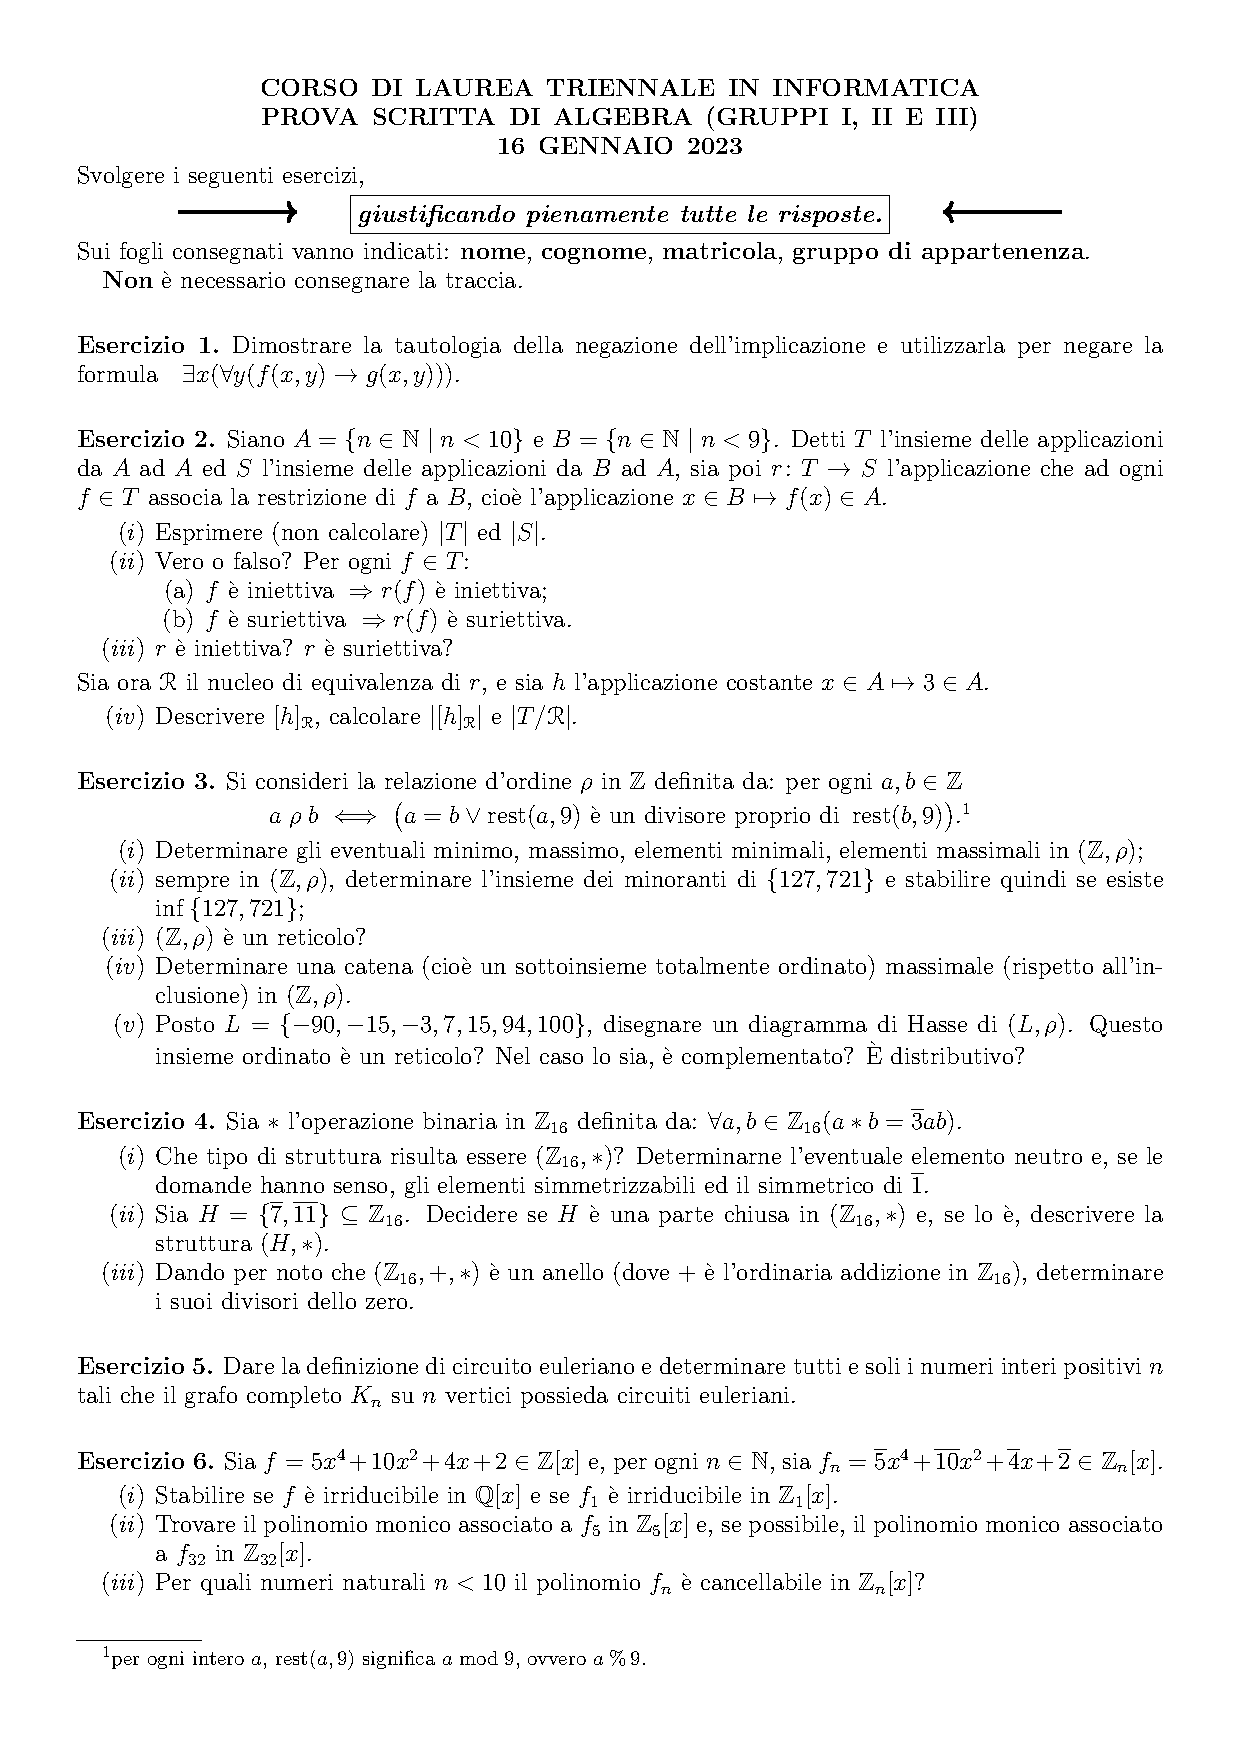
\includegraphics[scale=.85]{pdf/23-01-16.pdf}
\end{center}
\subsection*{Esercizio 1}
La tautologia della negazione dell'implicazione afferma che sono equivalenti le seguenti proposizioni:
\begin{align*}
	\neg(\alpha \implies \beta) \iff (\alpha \land \neg \beta)
\end{align*}
Infatti, sfruttando la tautologia dell'implicazione come disgiunzione abbiamo:
\begin{align*}
	\neg \bigl(\alpha \implies \beta \bigr) &\iff \neg \bigl( \neg \alpha \lor \beta \bigr) \\
	&\iff \neg (\neg \alpha) \land \neg \beta & \text{\textcolor{gray}{(Applicando la legge di De Morgan)}} \\
	&\iff \alpha \land \neg(\beta)
\end{align*}
Sfruttando questa tautologia allora abbiamo:
\begin{align*}
	\neg \biggl(\exists x \Bigl(\forall y \bigl( f(x,y) \implies g(x,y) \bigr)\Bigr)\biggr) &\iff \forall x \Bigl( \exists y \bigl( f(x,y) \land \neg g(x,y) \bigr)\Bigr)
\end{align*}
\subsection*{Esercizio 2}
\begin{enumerate}[label=(\textit{\roman*})]
	\item $|T|=|A|^{|A|}$ e $|S|=|A|^{|B|}$;
	\item \begin{enumerate}[label=(\alph*)]
		\item Sia $f$ iniettiva e supponiamo che $r(f)$ non sia iniettiva. Allora esistono $x,y \in B$ tali che $r(f)(x) =r(f)(y)$ e $x \neq y$. Ma, per definizione di restrizione, $r(f)(x) = f(x)$ e $r(f)(y)=f(y)$, quindi esistono $x,y \in A$ tali che $f(x)=f(y)$, il che va contro l'ipotesi che $f$ sia iniettiva. Quindi $r(f)$ non può non essere iniettiva se $f$ è iniettiva e l'implicazione risulta vera.
		\item Analogamente, sia $f$ suriettiva e supponiamo $r(f)$ non suriettiva. Ciò implica che esiste un $x \in A$ tale che $\overleftarrow{r(f)}(\{x\})=\emptyset$, ovvero non esiste $y \in B$ (e quindi di $A$) tale che $r(f)(y)=f(y)=x$. Quindi $f$ non risulterebbe suriettiva, contro le nostre ipotesi. Quindi, come nel punto precedente, si ha la veridicità dell'implicazione.
	\end{enumerate}
\item Essendo $|T| \geq |S|$ non possono esistere applicazioni iniettive da $T$ in $S$, quindi $r$ in particolare non può essere iniettiva. Infatti possono esistere applicazioni distinte da $A$ in $A$ che ammettono la stessa restrizione. Al contrario, per ogni restrizione è possibile costruire un prolungamento, per cui $r$ risulta essere una applicazione suriettiva.
\item Abbiamo:
\begin{align*}
	[h]_{\mathfrak{R}} &= \{ f \in T \; | \; r(f) = r(h)\} \\
	&= \{ f \in T \; | \; \forall x \in B (r(f)(x) = 3)\}
\end{align*}
Quindi in $[h]_{\mathfrak{R}}$ sono presenti le funzioni $f_{i}$ costruite ponendo:
\begin{align*}
	f_{i}: x \in A \mapsto \begin{cases*}
		3 & \iff x \in B \\
		i & \iff x \in A \setminus B = \{10\}
	\end{cases*}
\end{align*}
con $i$ che varia in $\{1,...,10\}$, per $i=3$ otteniamo proprio $h$. Quindi $|[h]_{\mathfrak{R}}| = 10$. Per il Teorema \ref{thm:teor_omomorfismo} abbiamo che $|T/{\mathfrak{R}}|=| im \ r| = |S|$ in quanto abbiamo detto che $r$ è suriettiva.
\end{enumerate}
\subsection*{Esercizio 3}
\begin{enumerate}[label=(\textit{\roman*})]
	\item Consideriamo la relazione di divisibilità in $\mathbb{Z}_{9}$, otteniamo il seguente diagramma di Hasse:
	\begin{center}
		\begin{tikzpicture}
			\node[circle,fill=black,inner sep=0pt,minimum size=3pt,label=below:{$[1]_{9}$}](1) at (0,0){};
			\node[circle,fill=black,inner sep=0pt,minimum size=3pt,label=below:{$[5]_{9}$}](5) at (-2,1){};
			\node[circle,fill=black,inner sep=0pt,minimum size=3pt,label=below:{$[3]_{9}$}](3) at (1,1){};
			\node[circle,fill=black,inner sep=0pt,minimum size=3pt,label=below:{$[4]_{9}$}](4) at (-0.5,2){};
			\node[circle,fill=black,inner sep=0pt,minimum size=3pt,label=below:{$[2]_{9}$}](2) at (-1,1){};
			\node[circle,fill=black,inner sep=0pt,minimum size=3pt,label=below:{$[6]_{9}$}](6) at (0.5,2){};
			\node[circle,fill=black,inner sep=0pt,minimum size=3pt,label=below:{$[7]_{9}$}](7) at (2,1){};
			\node[circle,fill=black,inner sep=0pt,minimum size=3pt,label=below:{$[8]_{9}$}](8) at (-0.5,3){};
			\node[circle,fill=black,inner sep=0pt,minimum size=3pt,label=above:{$[0]_{9}$}](0) at (0,4){};
			\draw[thin,black] (1)--(5);
			\draw[thin,black] (1)--(2);
			\draw[thin,black] (1)--(3);
			\draw[thin,black] (1)--(7);
			\draw[thin,black] (2)--(4);
			\draw[thin,black] (2)--(6);
			\draw[thin,black] (3)--(6);
			\draw[thin,black] (4)--(8);
			\draw[thin,black] (5)--(0);
			\draw[thin,black] (8)--(0);
			\draw[thin,black] (6)--(0);
			\draw[thin,black] (7)--(0);
		\end{tikzpicture}
	\end{center}
Portandoci su $(\mathbb{Z},\rho)$ osserviamo che ogni classe di resto contiene infiniti interi:
\begin{align*}
	[n]_{9} = \{ z \in \mathbb{Z} \; | \; \exists k \in \mathbb{Z}(z = 9k +n)\}
\end{align*}
Dal diagramma di Hasse disegnato si osserva che gli interi appartenenti alla classe di 1 modulo 9 risultano essere minimali in $(\mathbb{Z},\rho)$. Analogamente, gli interi appartenenti alla classe di 0 modulo 9 (i multipli di 9) risultano essere massimali in $(\mathbb{Z},\rho)$. Poiché due elementi appartenenti alla stessa classe sono in relazione $\rho$ se e solo se essi coincidono abbiamo che due elementi distinti nella stessa classe di resto risultano essere inconfrontabili e quindi non esiste un minimo ed un massimo in $(\mathbb{Z},\rho)$.
\item Osserviamo che sia $127 \in [1]_{9}$ che $721 \in [1]_{9}$\footnote{Basta applicare i criteri di divisibilità.}. Quindi i due elementi sono inconfrontabili, essendo $[1]_{9}$ il minimo in $(\mathbb{Z}_{9},\divides)$ non esistono minoranti di $\{127,721\}$ mentre esistono infiniti interi, a due a due inconfrontabili, maggioranti di $\{127,721\}$, quindi non esiste neanche un estremo superiore.
\item Per i motivi esposti al punto precedente $(\mathbb{Z},\rho)$ non risulta essere un reticolo.
\item Osservando il diagramma di Hasse di $(\mathbb{Z}_{9},\divides)$ osserviamo che è possibile individuare una catena massimale considerando le classi $[1]_{9}, \ [2]_{9}, \ [4]_{9}, \ [8]_{9}, \ [0]_{9}$. Spostandoci in $(\mathbb{Z},\rho)$ e prendendo un singolo elemento di ciascuna classe si ottiene un sottoinsieme massimale (rispetto all'inclusione). Ad esempio:
\begin{displaymath}
	\{10,11,13,17,18\}
\end{displaymath}
\item Abbiamo:
\begin{itemize}
	\item $-90 \in [0]_{9}$
	\item $-15 \in [3]_{9}$
	\item $-3 \in [6]_{9}$
	\item $7 \in [7]_{9}$
	\item $15 \in [6]_{9}$
	\item $94 \in [4]_{9}$
	\item $100 \in [1]_{9}$
\end{itemize}
Otteniamo così il seguente diagramma di Hasse:
\begin{center}
	\begin{tikzpicture}
		\node[circle,fill=black,inner sep=0pt,minimum size=3pt,label=below:{$100$}](a) at (0,0){};
		\node[circle,fill=black,inner sep=0pt,minimum size=3pt,label=below:{$7$}](b) at (-2,1){};
		\node[circle,fill=black,inner sep=0pt,minimum size=3pt,label=below:{$-15$}](c) at (0,1){};
		\node[circle,fill=black,inner sep=0pt,minimum size=3pt,label=below:{$94$}](d) at (2,1){};
		\node[circle,fill=black,inner sep=0pt,minimum size=3pt,label=below:{$15$}](e) at (0.5,1.5){};
		\node[circle,fill=black,inner sep=0pt,minimum size=3pt,label=below:{$-3$}](f) at (-0.5,1.5){};
		\node[circle,fill=black,inner sep=0pt,minimum size=3pt,label=above:{$-90$}](g) at (0,2.5){};
		\draw[thin,black] (a)--(b);
		\draw[thin,black] (a)--(c);
		\draw[thin,black] (a)--(d);
		\draw[thin,black] (c)--(e);
		\draw[thin,black] (c)--(f);
		\draw[thin,black] (d)--(g);
		\draw[thin,black] (b)--(g);
		\draw[thin,black] (e)--(g);
		\draw[thin,black] (f)--(g);
	\end{tikzpicture}
\end{center}
Tale insieme ordinato è un reticolo complementato, ma non è distributivo in quanto il sottoreticolo: $$(\{100,7,-15,94,-90\},\rho)$$ è isomorfo al reticolo trirettangolo:
\begin{center}
	\begin{tikzpicture}
		\node[circle,fill=black,inner sep=0pt,minimum size=3pt,label=below:{$100$}](a) at (0,0){};
		\node[circle,fill=black,inner sep=0pt,minimum size=3pt,label=below:{$7$}](b) at (-2,1){};
		\node[circle,fill=black,inner sep=0pt,minimum size=3pt,label=below:{$-15$}](c) at (0,1){};
		\node[circle,fill=black,inner sep=0pt,minimum size=3pt,label=below:{$94$}](d) at (2,1){};
		\node[circle,fill=black,inner sep=0pt,minimum size=3pt,label=above:{$-90$}](g) at (0,2.5){};
		\draw[thin,black] (a)--(b);
		\draw[thin,black] (a)--(c);
		\draw[thin,black] (a)--(d);
		\draw[thin,black] (c)--(g);
		\draw[thin,black] (d)--(g);
		\draw[thin,black] (b)--(g);
	\end{tikzpicture}
\end{center}
\end{enumerate}
\subsection*{Esercizio 4}
\begin{enumerate}[label=(\textit{\roman*})]
	\item L'operazione $\ast$ risulta essere associativa e commutativa. Infatti:
	\begin{align*}
		\forall x,y \in \mathbb{Z}_{16} \bigl( x \ast y = 3xy = 3yx = y \ast x \bigr)
	\end{align*}
Inoltre, presi $a,b,c \in \mathbb{Z}_{16}$ abbiamo:
\begin{align*}
	a \ast (b \ast c ) = a \ast (3bc) = 3a(3bc) = 9abc \\
	(a \ast b) \ast c = (3ab) \ast c = 3(3ab)c = 9abc
\end{align*}
Un elemento $t \in \mathbb{Z}_{16}$ è neutro in $(\mathbb{Z}_{16},\ast)$ se e solo se, per ogni $a \in \mathbb{Z}_{16}$ risulta:
\begin{align*}
	a \ast t = t \ast a  = 3ta = a &\iff 3t \equiv_{16} 1 \\
	&\iff t = \overline{11}
\end{align*}
Quindi $t= \overline{11}$ è il neutro del monoide $(\mathbb{Z}_{16},\ast)$. Un elemento $a \in \mathbb{Z}_{16}$ ammette simmetrico se e solo se esiste un $a' \in \mathbb{Z}_{16}$ tale che $a \ast a' = 11$, ovvero:
\begin{align*}
	3aa' \equiv_{16} 11 &\iff aa' \equiv_{16} 9 & \text{\textcolor{gray}{(Moltiplicando per 11 inverso di 3)}}
\end{align*}
Tale equazione ammette soluzione se e solo se $(a,16) \divides 9$. I divisori di $16$ minori di 9 sono $1, \ 2, \ 4, \ 8$ e solo divide 9. Possiamo concludere che se $a \in \{1,3,5,7,9\}$ allora $(a,16)=1 \divides 9$. Troviamo l'inverso di $x=\overline{1}$:
\begin{align*}
	x \ast x' \equiv_{16} 11 &\iff 3x' \equiv_{16} 11 \\
	&\iff x' \equiv_{16} 9
\end{align*}
	\item Risulta $7 \ast 7 = 3 \cdot 49 = 3 \cdot 1 = 3 \notin H$, quindi $H$ non è stabile in $(\mathbb{Z}_{16},\ast)$
	\item Un elemento $a \in \mathbb{Z}_{16}$ è divisore dello zero in $(\mathbb{Z}_{16},+,\ast)$ se esiste un elemento $b \in \mathbb{Z}_{16} \setminus \{\overline{0}\}$ tale che $ a \ast b=\overline{0}$. Abbiamo:
	\begin{align*}
		a \ast b = 3ab = \overline{0}
	\end{align*}
Essendo $3$ coprimo con $16$ abbiamo che tale elemento è simmetrizzabile e quindi cancellabile, per rendere il prodotto nullo abbiamo quindi bisogno che $ab = \overline{0}$. Tale richiesta si traduce quindi nella ricerca dei divisori dello zero in $(\mathbb{Z}_{16},\cdot)$ i quali sono tutti e soli gli elementi non invertibili, cioè $\mathbb{Z}_{16} \setminus \mathcal{U}(\mathbb{Z}_{16}) = \{0,2,4,6,8,10,12,14\}$.
\end{enumerate}
\subsection*{Esercizio 5}
Un circuito euleriano in un grafo è un percorso chiuso che attraversa ciascun arco del grafo esattamente una volta. Perché un grafo possa ammettere un circuito euleriano, deve soddisfare due condizioni:
\begin{itemize}
	\item Tutti i vertici devono avere grado pari
	\item Il grafo deve essere connesso
\end{itemize}
Un grafo completo $K_{n}$​ è un grafo in cui ogni coppia di vertici è connessa da un arco, quindi in particolare è un grafo connesso. Per un grafo completo, il grado di ogni vertice è $n−1$, poiché ogni vertice è collegato a tutti gli altri $n−1$ vertici. Quindi se $n-1$ deve essere pari ciò significa che $n$ è un numero dispari. Quindi ogni grafo completo con un numero dispari di vertici ammette circuiti euleriani.
\subsection*{Esercizio 6}
\begin{enumerate}[label=(\textit{\roman*})]
	\item Applicando il Criterio di Eisenstein con $p=2$ abbiamo che $2$ divide i coefficienti $a_{0},...,a_{3}$, 2 non divide $a_{n}=4$ e $p^{2}=4$ non divide 2. Quindi il polinomio $f$ è irriducibile in $\mathbb{Q}$ e di conseguenza, essendo associato al polinomio $f_{1} \in \mathbb{Z}_{1}[x] = \mathbb{Z}[x]$, è irriducibile anche in $\mathbb{Z}[x]$.
	\item Risulta $f_{5} = 4x+2$. Per trovare un polinomio monico associato risolviamo l'equazione $4x \equiv{5} 1$ che ha soluzione per $x=4$, quindi moltiplicando $f_{5}$ per 4 otteniamo:
	\begin{align*}
		4 \cdot f_{5} &= 4 \cdot (4x+2)   \\
		&= 16x + 8 \\
		&= x + 3
	\end{align*}
Analogamente, per $f_{32}$ risolviamo l'equazione $5x \equiv_{32} 1$ ottenendo $x=13$. Moltiplichiamo quindi $f_{32}$ per $x=\overline{13}$:
\begin{align*}
	13 \cdot f_{32} &= 13 \cdot \bigl(5x^{4} + 10x^{2}+4x+2\bigr) \\
	&= x^{4} +2x^{2} +20x + 26
\end{align*}
\item Un polinomio è cancellabile se e solo se $cd(f)$ è cancellabile nell'anello dei coefficienti. In questo caso, essendo $cd(f)=5$ un numero primo abbiamo che per ogni intero non nullo $n <10$ 5 è coprimo con $n$ e quindi simmetrizzabile, quindi cancellabile.
\end{enumerate}
\vfill
%\section{Esame del 16 giugno 2023}
%\begin{center}
%	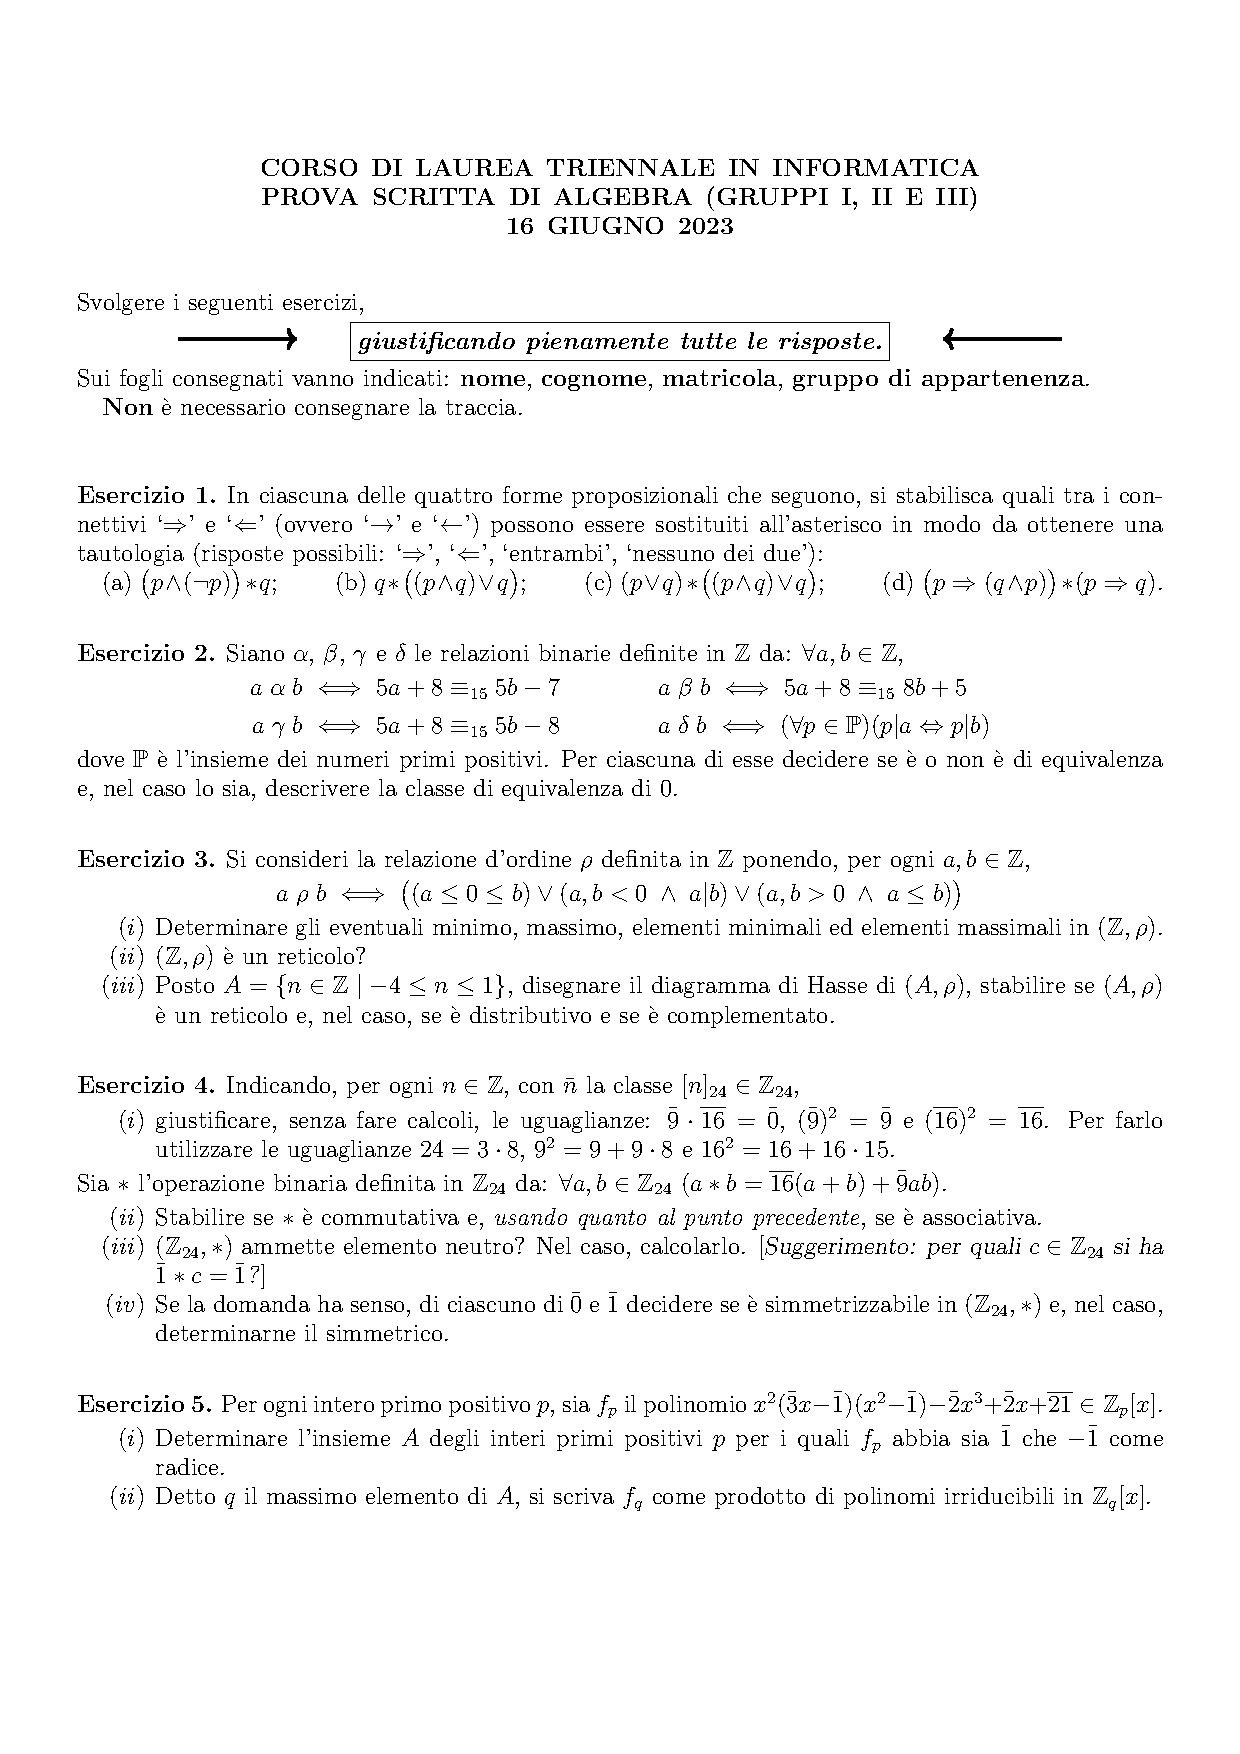
\includegraphics[scale=.85]{pdf/23-06-16.pdf}
%\end{center}
%\vfill
\section{Esame del 13 luglio 2023}
\begin{center}
	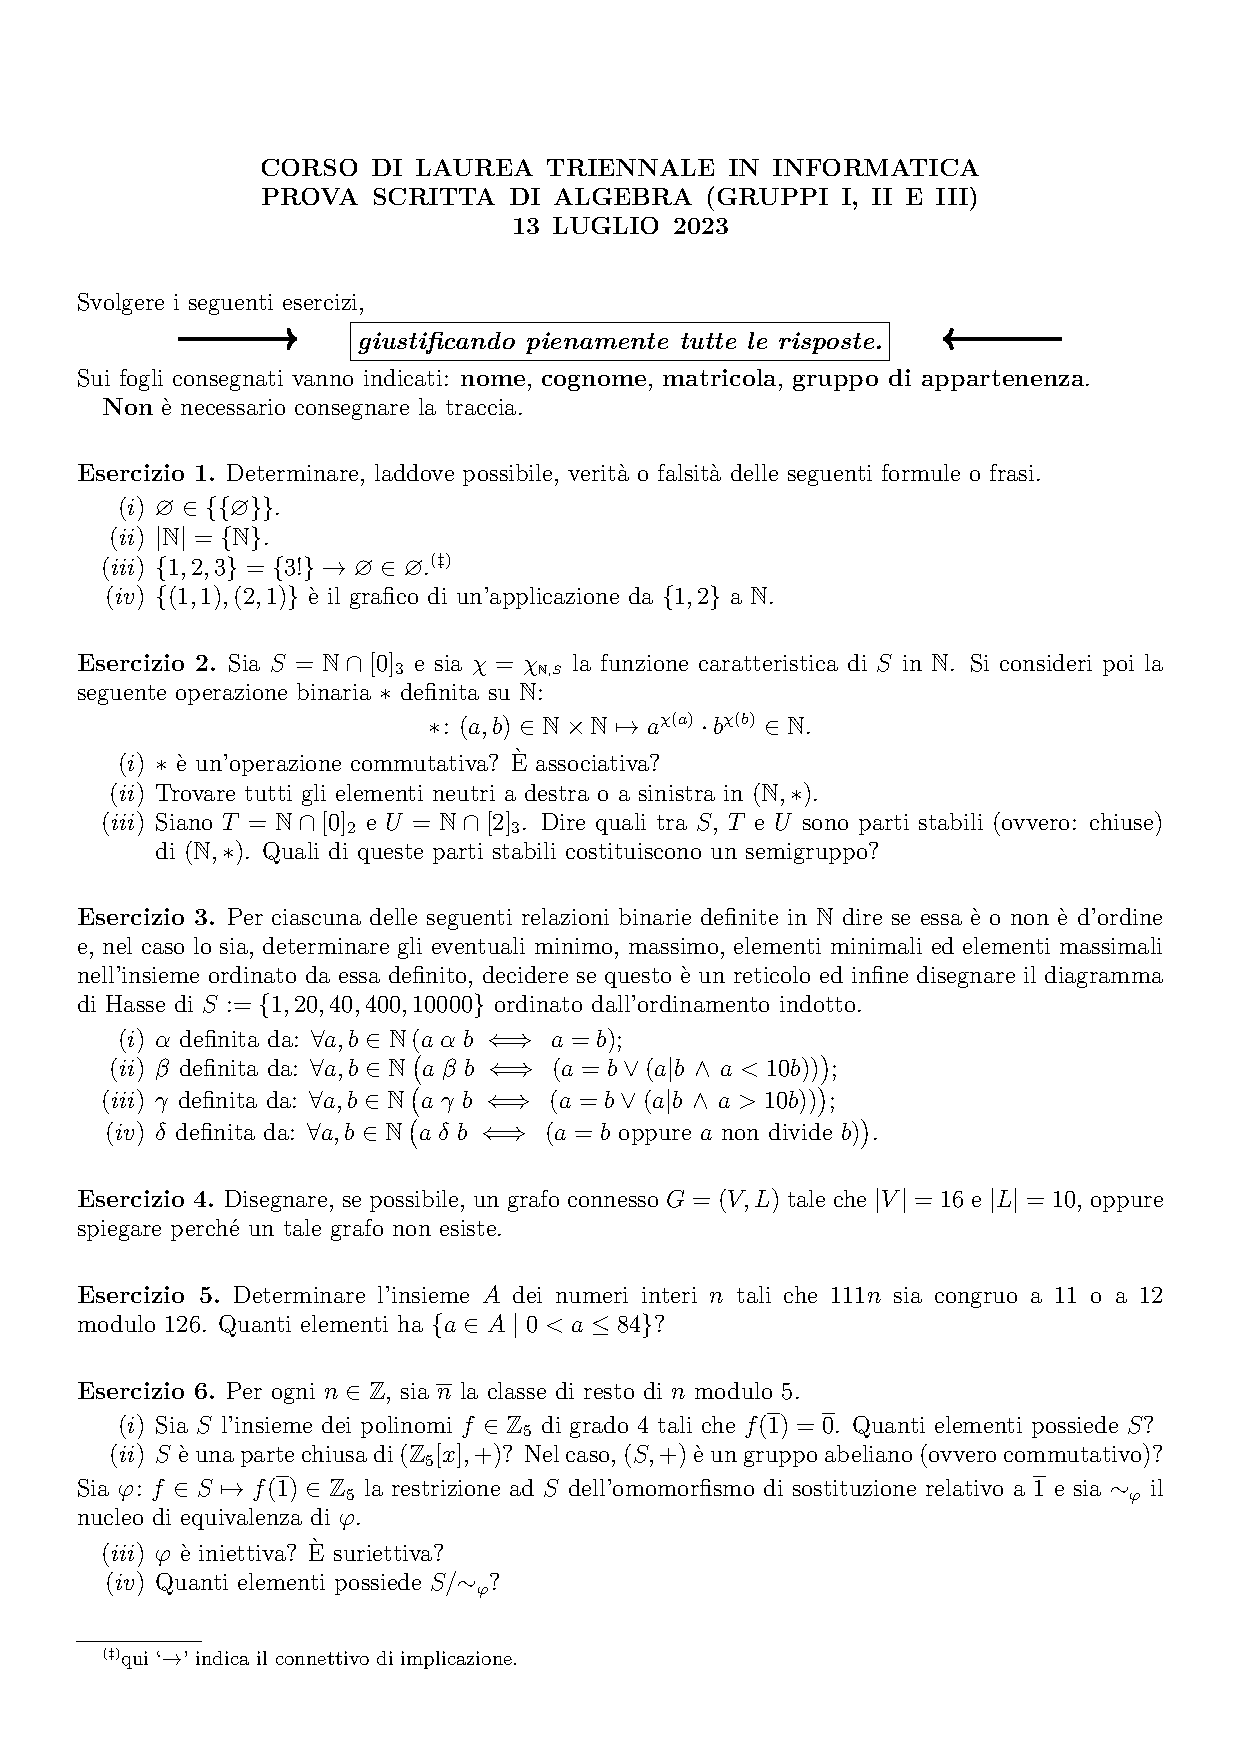
\includegraphics[scale=.85]{pdf/23-07-13.pdf}
\end{center}
\subsection*{Esercizio 1}
Abbiamo:
\begin{enumerate}[label=(\textit{\roman*})]
	\item \textbf{Falso}. L'insieme vuoto non è un elemento del singleton del singleton dell'insieme vuoto ma è tutt'al più una sua parte.
	\item \textbf{Falso}. Non ha senso confrontare un numero cardinale con un insieme. Il simbolo $|\mathbb{N}|$ indica infatti la cardinalità di $\mathbb{N}$, ovvero il numero dei suoi elementi, che è quantificabile col simbolo $\aleph$. Il simbolo $\{\mathbb{N}\}$ indica invece il singleton dell'insieme dei numeri naturali.
	\item \textbf{Vera}. Notiamo infatti che l'antecedente risulta essere una proposizione falsa in quanto l'insieme dei tre elementi $\{1,2,3\}$ non è uguale all'insieme $\{3!\}=\{6\}$. L'implicazione risulta quindi essere vera in quanto l'antecedente è falsa.
	\item \textbf{Vera}. Una applicazione $f: \{1,2\} \rightarrow \mathbb{N}$ è un'applicazione per la quale $\forall x \in \{1,2\}$  esiste un $n \in \mathbb{N}$ tale che $n=f(x)$. Il grafico $\{(1,1),(2,1)\}$ descrive in particolare l'applicazione costante $c_{1}$ che associa l'elemento 1 ad ogni elemento dell'insieme $\{1,2\}$.
\end{enumerate}
\subsection*{Esercizio 2}
L'insieme $S = \mathbb{N} \cap [0]_{3}$ è l'insieme dei multipli di $3$, ovvero:
\begin{align*}
	S =  \mathbb{N} \cap [0]_{3} = \{n \in \mathbb{N} \; | \; \exists k \in \mathbb{N} (n=3k)\} = 3\mathbb{N}
\end{align*}
L'applicazione caratteristica $\text{\Large\chi}_{\mathbb{N},S}$ restituisce 1 se $n \in 3\mathbb{N}$, 0 altrimenti. In particolare, $\forall n \in \mathbb{N}$:
\begin{align}\label{eq:130723_20}
	n^{\chi(a)} = 
	\begin{cases}
		a^{1} &\iff a \in 3\mathbb{N} \\
		a^{0} &\iff a \notin 3\mathbb{N}
	\end{cases}
\end{align}
\begin{enumerate}[label=(\textit{\roman*})]
	\item L'operazione $\ast$ è banalmente commutativa in quanto lo è la moltiplicazione ordinaria in $\mathbb{N}$. Per verificare l'associatività bisogna verificare che per ogni terna numerica $(a,b,c)$ di elementi di $\mathbb{N}$ risulti:
	\begin{align*}
		(a \ast b) \ast c = a \ast (b \ast c)
	\end{align*}
	Sviluppando il membro a sinistra otteniamo:
	\begin{align}
		(a \ast b) \ast c &= \bigl(a^{\chi(a)} \cdot b^{\chi(b)} \bigr) \ast c \nonumber \\
		&= \bigl( a^{\chi(a)} \cdot b^{\chi(b)}\bigr)^{\chi(a^{\chi(a)} \cdot b^{\chi(b)})} \cdot c^{\chi(c)} \label{eq:130723_21}
	\end{align}
	Mentre, sviluppando il membro a destra:
	\begin{align}
		a \ast (b \ast c) &= (b \ast c) \ast a & \text{\textcolor{gray}{(Applicando la commutatività di $\ast$)}} \nonumber \\
		&= \bigl(b^{\chi(b)}\cdot c^{\chi(c)}\bigr)^{\chi(b^{\chi(b)} \cdot c^{\chi(c)})} \cdot a^{\chi(a)} \label{eq:130723_22}
	\end{align}
	La verifica dell'uguaglianza di \ref{eq:130723_21} con \ref{eq:130723_22} deve essere fatta per casi:
	\begin{enumerate}
		\item Supponiamo il caso in cui $a,b,c \in 3\mathbb{N}$, in questo caso, applicando quanto osservato in \ref{eq:130723_20} otteniamo:
		\begin{align*}
			(a \ast b) \ast c &= \bigl( a^{\chi(a)} \cdot b^{\chi(b)}\bigr)^{\chi(a^{\chi(a)} \cdot b^{\chi(b)})} \cdot c^{\chi(c)} & \text{\textcolor{gray}{
					(Osservando che $ab \in 3\mathbb{N}$)}}\\
			&= (a\cdot b) \cdot c = (ab)c 
		\end{align*}
		e analogamente:
		\begin{align*}
			a \ast (b \ast c) &= \bigl(b^{\chi(b)}\cdot c^{\chi(c)}\bigr)^{\chi(b^{\chi(b)} \cdot c^{\chi(c)})} \cdot a^{\chi(a)} \\
			&= (b \cdot c) \cdot a = a(bc)
		\end{align*}
		\item Siano ora $a,b,c \notin 3\mathbb{N}$. Allora:
		\begin{align*}
			(a \ast b) \ast c = (1 \cdot 1)^{0} \cdot 1 = 1 \\
			(a \ast b) \ast c =  (1 \cdot 1)^{0} \cdot 1 = 1
		\end{align*}
		\item Sia uno tra $a,b,c$ non appartenente a $3\mathbb{N}$. Senza ledere di generalità, sia esso $c$. Abbiamo quindi:
		\begin{align*}
			(a \ast b) \ast c = (a \cdot b) ^{1} \cdot 1 = ab \\
			a \ast (b \ast c) = a(b \cdot 1)^{1} = ab
		\end{align*}
		\item Siano due elementi non appartenenti a $3\mathbb{N}$, siano essi $b,c$, allora:
		\begin{align*}
			(a \ast b) \ast c = (a \cdot 1)^{1} = a \\
			a \ast (b \ast c) = a \cdot (1 \cdot 1)^{0} = a
		\end{align*}
	\end{enumerate}
	In ogni caso il membro a destra e a sinistra coincidono e quindi $\ast$ risulta associativa.
	\item Per esistere elemento neutro rispetto all'operazione $\ast$ deve esistere un $t \in \mathbb{N}$ tale che, per ogni $n \in \mathbb{N}$, garantisca che $n \ast t = t \ast n = n$. Un tale $t$ non può esistere in quanto:
	\begin{align*}
		\forall n \in \mathbb{N} \bigl(n \ast t = n &\iff n^{\chi(n)} \cdot t^{\chi(t)} = n \\
		&\iff n^{\chi(n)} = n \land t^{\chi(t)}=1 \\
		&\iff (n \in 3\mathbb{N}) \land (t \notin 3\mathbb{N}) \bigr)
	\end{align*}
	Dato che non può esistere un tale $t$ che sia neutro per ogni naturale possiamo concludere affermando la sua non esistenza.
	\item Abbiamo $T=2\mathbb{N}$ e $U=\{n \in \mathbb{N} \; | \; \exists k \in \mathbb{N}(n=3k+2)\}$. Una parte $X \subseteq \mathbb{N}$ si dice stabile se, e solo se, per ogni $(a,b) \in X \times X$ si abbia $a \ast b \in X$.
	\begin{itemize}
		\item Presi ad esempio $a=14$ e $b=16$ elementi di $T$ abbiamo:
		\begin{align*}
			14 \ast 16 &= 14^{\chi(14)} \cdot 16^{\chi(16)} \\
			&= 14^{0} \cdot 16^{0} = 1 \notin T
		\end{align*}
		Quindi $T$ non è stabile.
		\item Presi $a=5$ e $b=7$ elementi di $U$, abbiamo:
		\begin{align*}
			5 \ast 7 &= 5^{\chi(5)} \cdot 7^{\chi(7)} \\
			&= 1 \notin U
		\end{align*}
		Quindi $U$ non è stabile.
		\item Presi due elementi $a,b \in S$ abbiamo:
		\begin{align*}
			a \ast b = a^{\chi(a)} \cdot b^{\chi(b)} \\
			&= a \cdot b \in S
		\end{align*}
		Quindi il semigruppo $(S,\ast)$ risulta stabile rispetto a $\ast$.
	\end{itemize}
\end{enumerate}
\subsection*{Esercizio 3}
\begin{enumerate}[label=(\textit{\roman*})]
	\item La relazione $\alpha$ coincide con la relazione identica $id_{\mathbb{N}}$ che è una relazione d'ordine. In $(\mathbb{N},\alpha)$ tutti i numeri sono sia minimali che massimali. Non esistono minimo e massimo. Non potendo definire, per ogni coppia di elementi $(n,m)$ l'infimo ed il supremo della parte $\{a,b\}$ l'insieme ordinato non costituisce un reticolo.
	Presa la parte $S=\{1,20,40,400,10000\}$ abbiamo il seguente diagramma di Hasse:
	\begin{center}
		\begin{tikzpicture}
			\filldraw[black] (0,0) circle(2pt) node[anchor=north]{1};
			\filldraw[black] (1,0) circle(2pt) node[anchor=north]{20};
			\filldraw[black] (2,0) circle(2pt) node[anchor=north]{40};
			\filldraw[black] (3,0) circle(2pt) node[anchor=north]{400};
			\filldraw[black] (4,0) circle(2pt) node[anchor=north]{10000};
		\end{tikzpicture}
	\end{center}
	\item  Per verificare che $\beta \in OL(\mathbb{N})$ verifichiamo che essa sia riflessiva, antisimmetrica e transitiva:
	\begin{enumerate}
		\item Chiaramente $\forall a \in \mathbb{N}$ risulta $a \ \beta \ a $ in quanto $a=a$ e questo è sufficiente per garantire la corrispondenza di un numero con se stesso.
		\item Siano $a,b \in \mathbb{N}$ tali che $a \ \beta \ b$ e $b \ \beta \ a$:
		\begin{align}
			\begin{cases}
				a \ \beta \ b &\iff a=b \lor (a \divides b \land a < 10b) \\
				b \ \beta \ a &\iff b=a \lor (b \divides a \land b < 10a)
			\end{cases}
		\end{align}
		Nel caso gli elementi coincidano l'antisimmetria di $\beta$ è una conseguenza triviale. Se $a \divides b \land a <10b$ e $b \divides a \land b<10a$ allora, in particolare, gli elementi risultano essere elementi associati in $\mathbb{N}$ e quindi devono coincidere per forza.
		\item Siano $a,b,c \in \mathbb{N}$ elementi tali che $a \ \beta \ b$ e $b \ \beta \ c$. Allora, se $a=b$ e $b=c$ allora $a=c$ e quindi $ a \ \beta \ c$. Altrimenti, se $a \divides b \land a <10b$ e $b \divides c \land b<10c$ allora possiamo scrivere $b=ka$ per un opportuno $k \in \mathbb{N}$ e $c=mb=m(ka)=a(km)$. Quindi $a \divides c$ e inoltre possiamo eseguire la maggiorazione $a < 10b < 100c$. Quindi vale sicuramente $a < 10c$ e $a \ \beta \ c$. Quindi $\beta \in OL(\mathbb{N})$.	
	\end{enumerate}
	L'elemento 1 risulta essere il minimo in $(\mathbb{N},\beta)$ in quanto, $\forall n \in \mathbb{N}(1 \ \beta \ n)$. Dato che per ogni $a,b$ esiste sempre un elemento $n \in \mathbb{N}$ tale che $n \cdot a > b$, possiamo dire che in  $(\mathbb{N},\beta)$ non esistono elementi massimali e dunque un massimo. L'insieme ordinato risulta essere un reticolo in quanto per ogni parte $\{a,b\}$ possiamo trovare l'infimo ed il supremo che è dato dal massimo comun divisore e dal minimo comune multiplo di $(a,b)$. In particolare $(S,\beta)$ risulta essere un insieme totalmente ordinato. Si ottiene quindi la catena:
	\begin{center}
		\begin{tikzpicture}
			\filldraw[black] (0,0) circle(2pt) node[anchor=north]{1};
			\filldraw[black] (0,1) circle(2pt) node[anchor=north]{20};
			\filldraw[black] (0,2) circle(2pt) node[anchor=north]{40};
			\filldraw[black] (0,3) circle(2pt) node[anchor=north]{400};
			\filldraw[black] (0,4) circle(2pt) node[anchor=north]{10000};
			\draw[black](0,0)--(0,1)--(0,2)--(0,3)--(0,4);
		\end{tikzpicture}
	\end{center}
	\item La relazione $\gamma$ coincide con la relazione $\alpha$ in quanto osserviamo che la proposizione $(a \divides b \land a > 10b)$ risulta sempre falsa. Infatti un divisore non può essere maggiore di un multiplo dell'elemento che divide. Resta però la condizione di uguaglianza la quale, come visto nel primo punto, risulta essere una relazione d'ordine.
	\item La relazione $\delta$ non risulta essere una relazione d'ordine in $\mathbb{N}$ in quanto non soddisfa la proprietà antisimmetrica. Infatti presi $a,b \in \mathbb{N}$ tali che $a \ndivides b$ e $b \ndivides a$, ovvero $a \ \delta \ b$ e $b \ \delta \ a$, ciò non implica che sia necessariamente $a=b$. Ad esempio abbiamo $2 \ \delta \ 5$ e $5 \ \delta \ 2$ in quanto $2 \ndivides 5$ e $5 \ndivides 2$ ma $2 \neq 5$.
\end{enumerate}

\subsection*{Esercizio 4}
Un grafo si dice connesso se per ogni coppia di vertici esiste un cammino. Se il numero di vertici è pari a 16 ciò significa che devono esistere almeno 15 lati. Per questo motivo non è possibile disegnare un grafo connesso con 16 vertici e 10 lati.
\subsection*{Esercizio 5}
Calcoliamo il Massimo Comun Divisore tra 111 e 126.
\begin{align*}
	111 = 3 \cdot 37 \\
	126 = 2 \cdot 3^{2} \cdot 7
\end{align*}
L'equazione $111n \equiv_{126} 11$ non ammette soluzioni in quanto $MCD(111,126)=3$ non divide 11, mentre $111n \equiv_{126} 12$ risulta essere una equazione compatibile. Dividendo tutti i termini per 3 si ottiene l'equazione equivalente ridotta:
\begin{align*}
	\frac{111}{3}n \equiv_{\frac{126}{3}} \frac{12}{3} = 37n \equiv_{42} 4
\end{align*}
E vale $MCD(37,42)=1$. Cerchiamo una combinazione lineare $37u+42v=1$. Applicando l'algoritmo delle divisioni successive si ottiene:
\begin{align*}
	42 = 37 \cdot 1 + 5 \\
	37 = 5 \cdot 7 + 2 \\
	5 = 2 \cdot 2 + 1 \\
	2 = 1 \cdot 2 + 0
\end{align*}
Da queste relazioni otteniamo:
\begin{align}
	5 = 42 +(-1)37 \\
	2 = 37 +(-7)5 \\
	1 = 5 + (-2)2
\end{align}
Possiamo dunque esprimere 1 come:
\begin{align*}
	1 &= 5 - 4 \\
	&= \bigl(42-37\bigr)+(-2)\bigl(37-35\bigr) \\
	&= 42 - 37 +(-2)37+(14)5 \\
	&= 42+ (-3)37 +(14)\bigl(42+(-1)37\bigr) \\
	&= 42 + (-3)37 + (14)42+(-14)37 \\
	&= (15)42 + (-17)37
\end{align*}
Moltiplicando tale combinazione lineare per 4 si ottiene:
\begin{align*}
	4 = (60)42 + (-68)37
\end{align*}
Quindi $u=[-68]_{42}=[16]_{42}$ è soluzione dell'equazione. L'insieme $A=\{[16]_{42}\}$ e vale $\{a \in A \; | \; 0 \leq a \leq 84\} = \{16,58\}$.
\subsection*{Esercizio 6}
\begin{enumerate}[label=(\textit{\roman*})]
	\item L'insieme $S$ è costituito dai polinomi $f \in \mathbb{Z}_{5}$ di grado 4 tali che $f(\overline{1})=0$. Un polinomio di grado 4 in $\mathbb{Z}_{5}[x]$ può essere scritto come:
	\begin{align*}
		a_{4}x^{4}+a_{3}x^{3}+a_{2}x^{2}+a_{1}x+a_{0}
	\end{align*}
	Con $a_{4} \neq \overline{0}$, altrimenti non sarebbe un polinomio di quarto grado. Imporre che $f(\overline{1})=0$ è equivalente a dire che:
	\begin{align*}
		a_{4}+a_{3}+a_{2}+a_{1}+a_{0} = 0
	\end{align*}
	La domanda della conta degli elementi di $S$ può essere rivista come il conteggio di tutte le possibili combinazioni degli elementi $a_{i}$ con $i \in \mathbb{Z}_{5}$ tali che $\sum_{i=0}^{4} a_{i}=0$ e tale che $a_{4} \neq \overline{0}$.
	Per ciascuno di questi casi, stiamo essenzialmente chiedendo in quanti modi possiamo scegliere $4$ numeri da $\{0, 1, 2, 3, 4\}$ la cui somma sia un valore specifico. Abbiamo quindi:
	\begin{itemize}
		\item Se $a_{4}=1$, deve essere $a_{3}+a_{2}+a_{1}+a_{0}=4$;
		\item Se $a_{4}=2$, deve essere $a_{3}+a_{2}+a_{1}+a_{0}=3$;
		\item Se $a_{4}=3$, deve essere $a_{3}+a_{2}+a_{1}+a_{0}=2$;
		\item Se $a_{4}=4$, deve essere $a_{3}+a_{2}+a_{1}+a_{0}=1$.
	\end{itemize}
	Per ogni caso, il numero di combinazioni con ripetizione di $4$ elementi presi dall'insieme $\mathbb{Z}_{5}$ che diano somma $k$ con $k \in \{4,3,2,1\}$ è dato da:
	\begin{align*}
		\sum_{k=1}^{4} \binom{4+k-1}{i} &= \binom{4+1-1}{1}+\binom{4+2-1}{2}+\binom{4+3-1}{3}+\binom{4+4-1}{4} \\
		&= 4 + 10 + 20 + 35 \\
		&= 69
	\end{align*}
	\item $(S,+)$ è una parte chiusa. Infatti, presi due polinomi $s,q \in S$ allora $s+q$ calcolato in $\overline{1}$ è equivalente a $s(1)+q(1)=0$. $(S,+)$ non risulta essere abeliano in quanto il polinomio nullo non è un polinomio di grado 4.
	\item Osserviamo che per ogni $f \in S\bigl(\varphi(f)= f(\overline{1})=\overline{0}\bigr)$, e $\varphi$ risulta essere una applicazione costante. Quindi $\varphi$ non è iniettiva e non è suriettiva. 
	\item Essendo costante $\varphi$ il suo nucleo di equivalenza coincide con la relazione totale in $S$. Quindi $S/{\sim_{\varphi}} = S/{\tau_{S}} = \{S\}$, ed esiste un'unica classe di equivalenza.
\end{enumerate}
\vfill
%\section{Esame del 4 ottobre 2023}
%\begin{center}
%	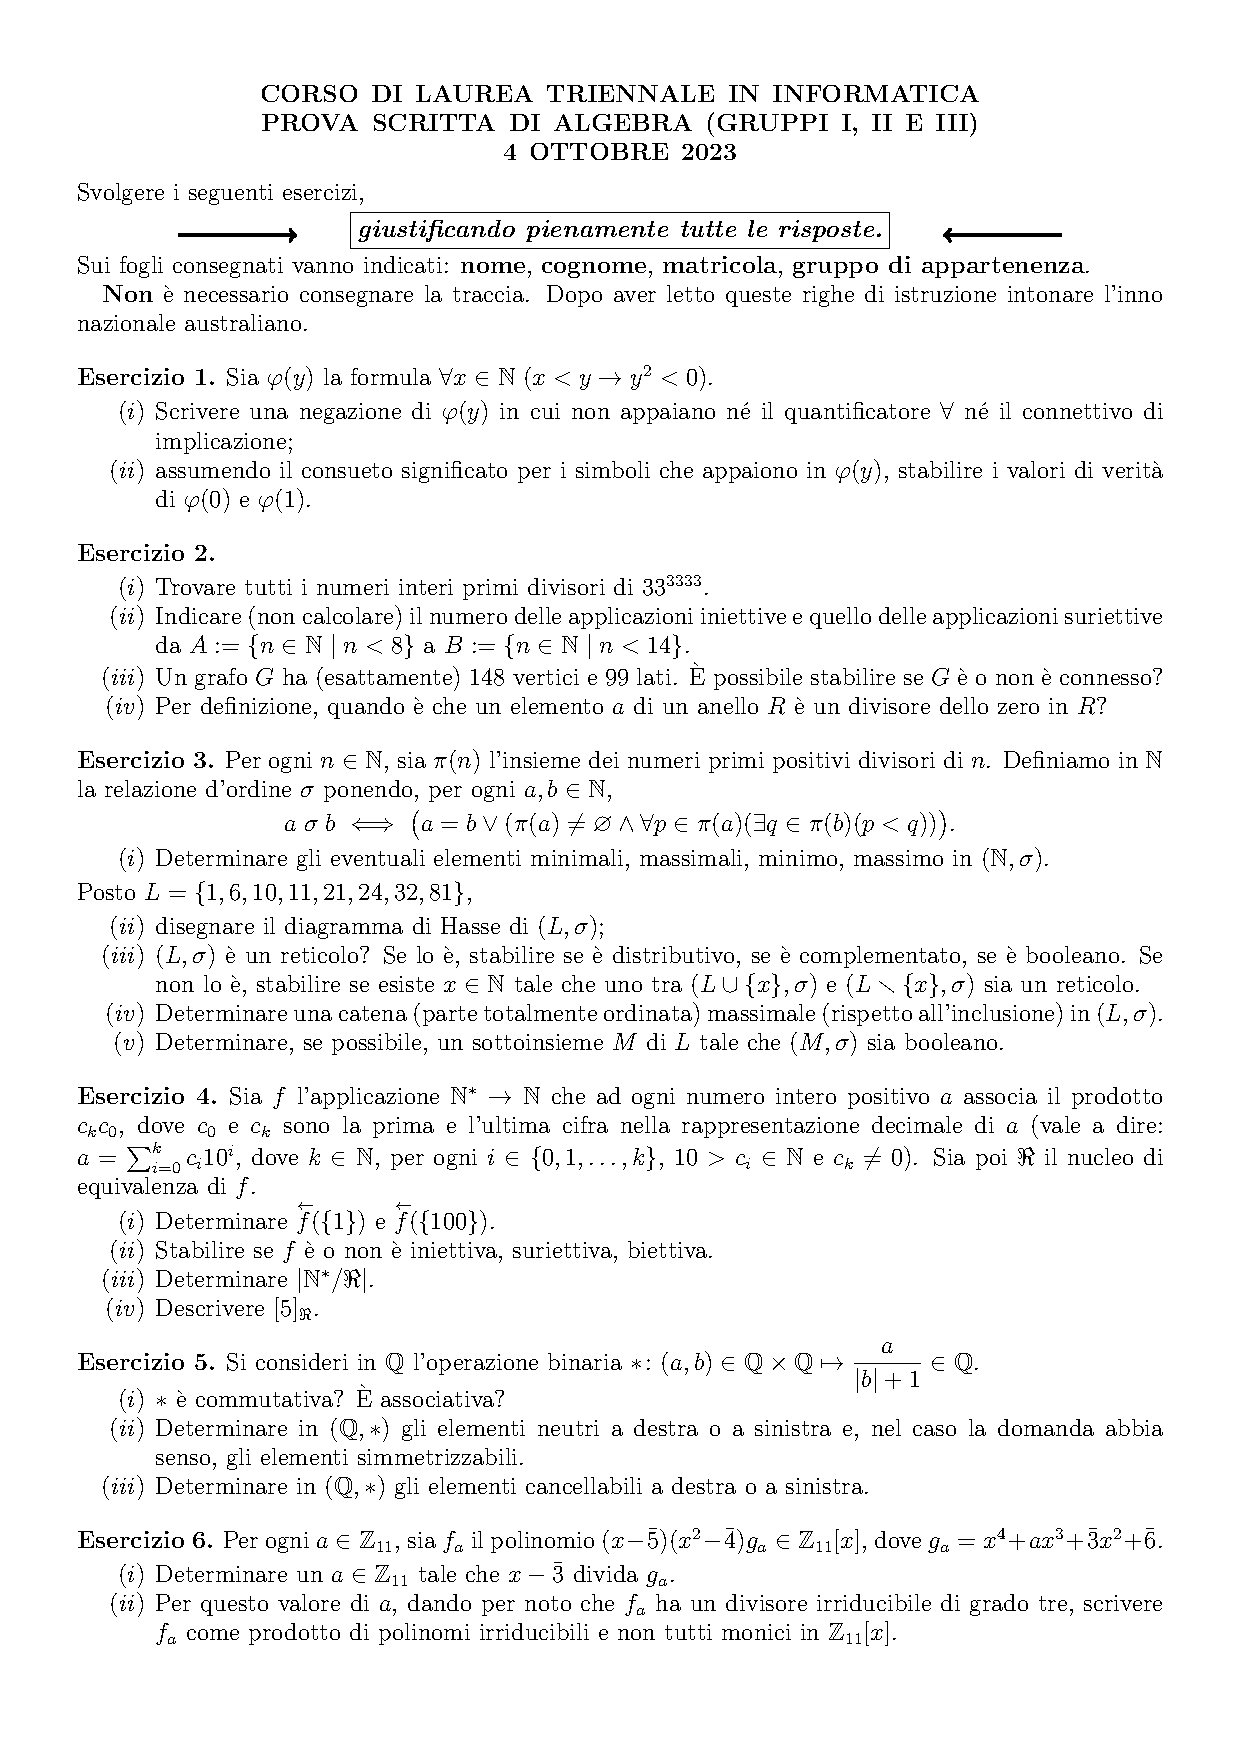
\includegraphics[scale=.85]{pdf/23-10-04.pdf}
%\end{center}
\section{Esame del 15 gennaio 2024}
\begin{center}
	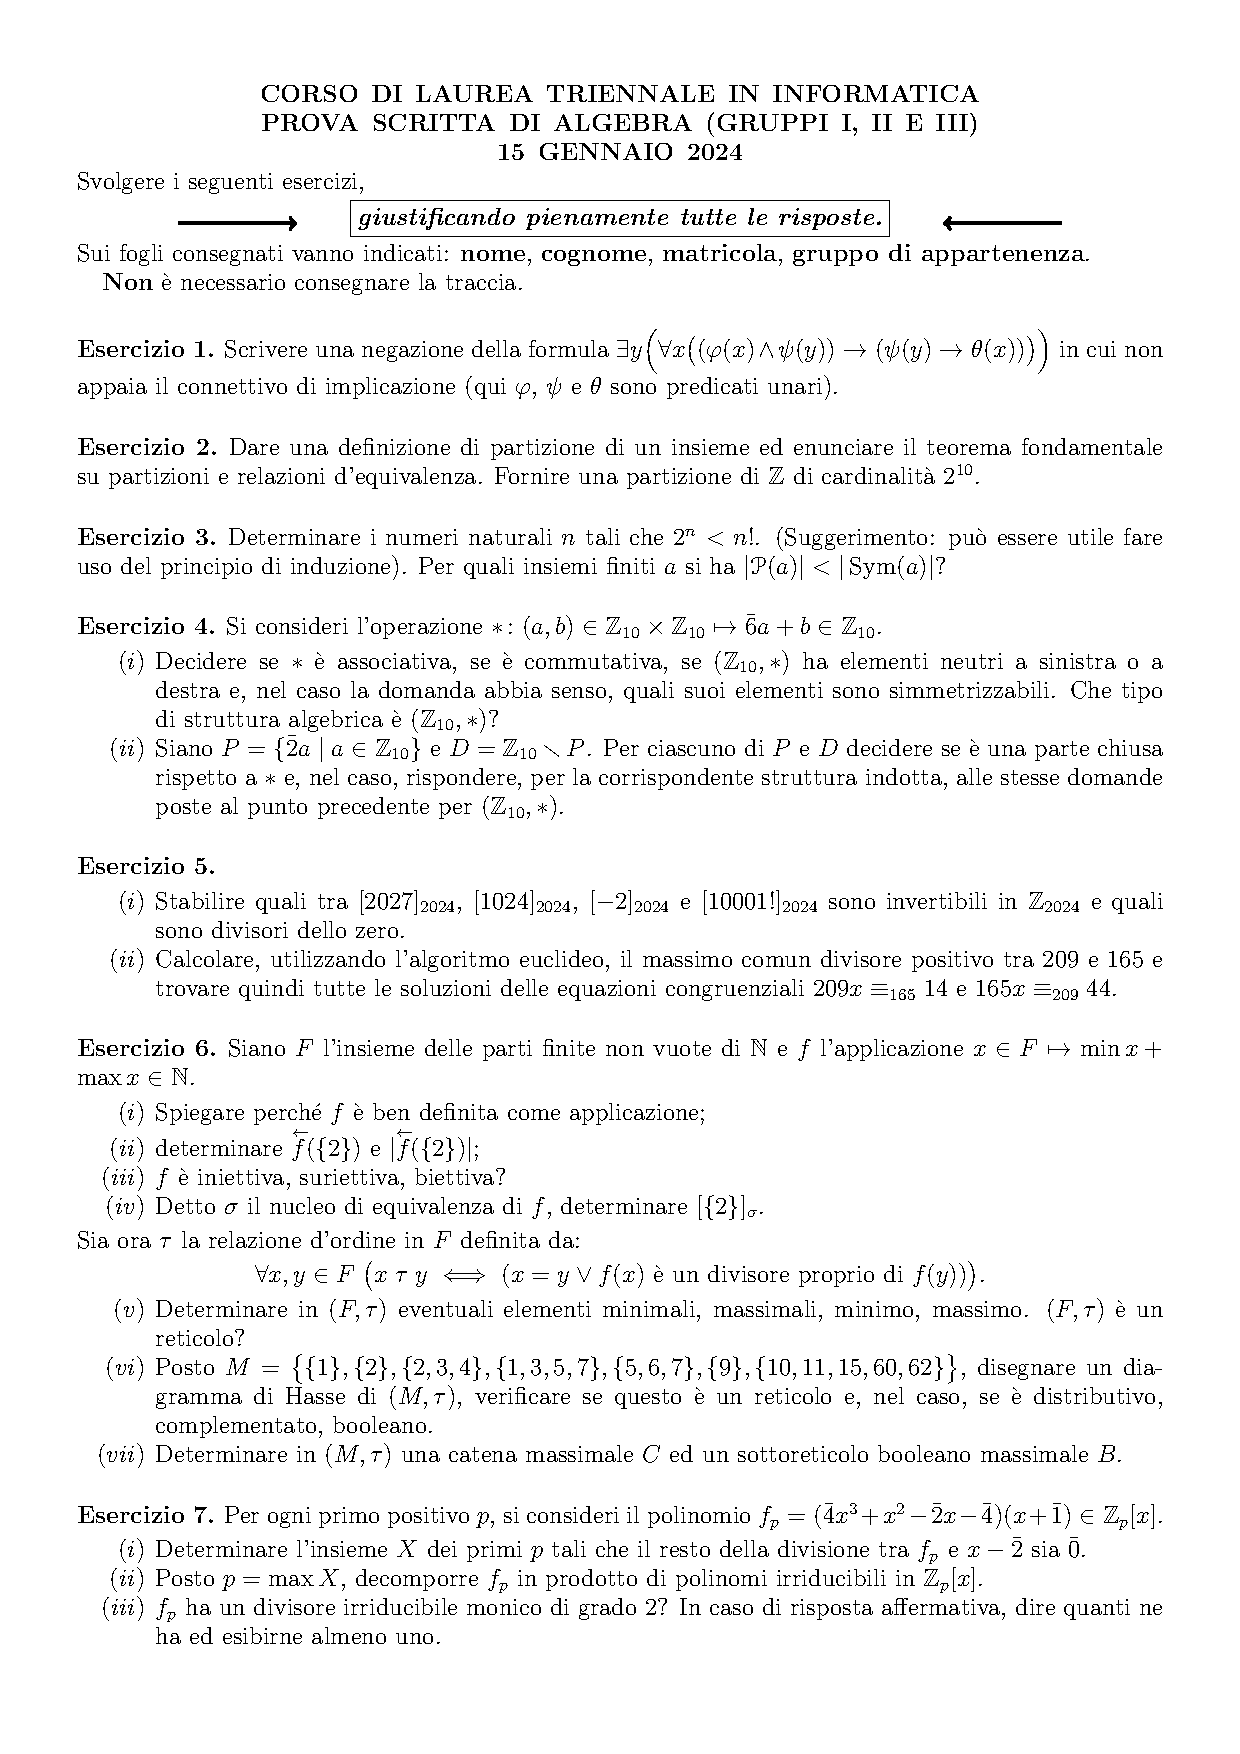
\includegraphics[scale=.85]{pdf/Traccia_150124}
\end{center}
\subsection*{Esercizio 1}
Applicando la Proposizione \ref{prop:negazione_quantificatori} si ottiene:
\begin{align*}
	\neg \Biggl(\exists y \biggl(\forall x \biggl( \bigl( \varphi(x) \land \psi(y)\bigr)	\implies \bigl(	\psi(y) \implies \theta(x) \bigr)\biggr)\biggr)
	\Biggr) &\iff	\forall y \Biggl(\neg \biggl(\forall x \Bigl( \bigl( \varphi(x) \land \psi(y)		\bigr) \implies \bigl(\psi(y) \implies \theta(x)\bigr)\Bigr) \biggr) \Biggr) \\
	&\iff \forall y 
	\biggl( \exists x \Bigl( \neg  \bigl( \varphi(x) \land \psi(y)\bigr) \implies \bigl(	\psi(y) \implies \theta(x)	\bigr) 	\Bigr)	\biggr) \\
\end{align*}
Poniamo $\alpha \coloneqq \varphi(x) \land \psi(y)$ e $\beta \coloneqq \psi(y) \implies \theta(x)$ e vale, per la Proposizione \ref{prop:negazione_implicazione}:
\begin{align*}
	\neg (\alpha \implies \beta) &\iff \alpha \land \neg (\beta) \\
	&\iff \bigl( \varphi(x) \land \psi(y)\bigr) \land \neg \bigl(\psi(y) \implies \theta(x)\bigr) \\
	&\iff \bigl( \varphi(x) \land \psi(y)\bigr) \land \bigl(\psi(y) \land \neg (\theta(x))\bigr) \\
	&\iff \varphi(x) \land \psi(y) \land \psi(y) \land \neg \bigl(\theta(x)\bigr) \\
	&\iff \varphi(x) \land \psi(y) \land \neg \bigl(\theta(x)\bigr)
\end{align*}
Sostituiamo quindi la formula ottenuta:
\begin{align*}
	\forall y 
	\biggl( \exists x \Bigl( \varphi(x) \land \psi(y) \land \neg \bigl(\theta(x)\bigr)	\Bigr)	\biggr) \\
\end{align*}
\subsection*{Esercizio 2}
Una partizione di un insieme $X$ è un insieme $\mathcal{F}$ di non vuote di $X$ tale insieme, a due a due disgiunte, la cui unione unaria è tutto $X$, ovvero $\bigcup \mathcal{F} = X$. Il Teorema fondamentale su partizioni e relazioni di equivalenza afferma che esiste una corrispondenza biunivoca tra l'insieme delle partizioni di un insieme $A$ e l'insieme delle equivalenze $Eq(A)$, cioè ogni partizione è un insieme quoziente e viceversa. Una partizione di $\mathbb{Z}$ di cardinalità $2^{10}$ è dato dall'insieme quoziente di $\mathbb{Z}$ rispetto alla congruenza modulo $2^{10}$.
\subsection*{Esercizio 3}
Per induzione si dimostra che per ogni $n \geq 4 \bigl( 2^{n} < n! \bigr)$. Infatti:
\begin{itemize}
	\item Se $n=0$ abbiamo $2^{0}=1 = 0!$;
	\item Se $n=1$ abbiamo $2^{1} = 2 > 1 = 1!$;
	\item Se $n=2$ abbiamo $2^{2} = 4 > 2 = 2!$;
	\item Se $n=3$ abbiamo $2^{3} = 8 > 6 = 3!$;
	\item Se $n=4$ abbiamo $2^{4} = 16 < 24 = 4!$;
\end{itemize}
Sia quindi $n>4$ e supponiamo l'asserto vero. Dimostriamo quindi che $2^{n+1}<(n+1)!$. Si ha:
\begin{align*}
	2^{n+1} = 2^{n} \cdot 2
\end{align*}
e 
\begin{align*}
	(n+1)! = (n+1)n!
\end{align*}
Dato che per ipotesi induttiva $2^{n}<n!$ e, dato che $n>4$, sicuramente $2 < n+1$, quindi è lecito eseguire la maggiorazione:
\begin{align*}
	2^{n+1} = 2^{n} \cdot 2 < n! (n+1) = (n+1)!
\end{align*}
Per quanto appena visto possiamo affermare che $|\mathcal{P}(a)| < |Sym(a)|$ per tutti gli insiemi con almeno 4 elementi.
\subsection*{Esercizio 4}
\begin{enumerate}[label=(\textit{\roman*})]
	\item Per ogni terna di elementi $a,b,c \in \mathbb{Z}_{10}$:
	\begin{align*}
		a \ast (b \ast c) &= a \ast (6b +c) \\
		&= 6a +6b+c
	\end{align*}
	e:
	\begin{align*}
		(a \ast b) \ast c &= (6a+b) \ast c \\
		&= 6(6a+b) + c \\
		&= 36a + 6b + c \\
		&= 6a + 6b+c
	\end{align*}
	Quindi $\ast$ è associativa. Siano $a,b \in \mathbb{Z}_{10}$:
	\begin{align*}
		a \ast b = 6a +b \neq  6b +a  = b \ast a
	\end{align*}
	Infatti, presi $a=1$ e $b=0$ abbiamo $a \ast b = 6$ e $b \ast a = 1$. Quindi $\ast$ non è commutativa. Cerchiamo un eventuale neutro a sinistra. Un siffatto elemento, composto a sinistra con qualunque elemento di $\mathbb{Z}_{10}$ deve restituire l'elemento stesso. Ossia:
	\begin{align*}
		\forall x \in \mathbb{Z}_{10} \bigl( t \ast x = x &\iff 6t + x = x  \\
		&\iff 6t = 0 \bigr)
	\end{align*}
	Gli unici $t \in \mathbb{Z}_{10}$ che sono soluzioni di tale equazione risultano essere $t=\overline{5}$ e $t=\overline{0}$. Questi sono gli unici possibili elementi che possono essere neutri a destra. Osserviamo però che, preso un $a \in \mathbb{Z}_{10}$:
	\begin{align*}
		a \ast 0 = 6a  + 0 = a &\iff 5a \equiv_{10} 0 \\ 
		&\iff a = 6 \lor a = 0 
	\end{align*}
	e:
	\begin{align*}
		a \ast 5 = 6a  + 5 = a &\iff 5a \equiv_{10} 5 \\
		&\iff a = \overline{9} \lor a= \overline{1}  \lor a=\overline{3} \lor a = \overline{5} \lor a = \overline{7}
	\end{align*}
	Quindi non risultano essere neutri per tutti gli elementi di $\mathbb{Z}_{10}$.
	\item Abbiamo $P=\{\overline{0},\overline{2},\overline{4},\overline{6},\overline{8}\}$ e $D = \{\overline{1},\overline{3},\overline{5},\overline{7},\overline{9}\}$. Siano $n,m$ due elementi di $\mathbb{Z}_{10}$ e consideriamo i rispettivi elementi $2n$ e $2m$ in P. Allora:
	\begin{align*}
		2n \ast 2m = 12 n + 2m = 2(6n+3m) \in P
	\end{align*}
	Analogamente, un elemento di $D$ è scrivibile come $2n+1$ e abbiamo:
	\begin{align*}
		(2n+1) \ast (2m+1) &= 12n+ 6 + 2m+1  \\
		&= 2(6n+m+3) +1 \in D
	\end{align*}
	Quindi sia $P$ che $D$ sono parti chiuse rispetto a $\ast$. Per le conclusioni del punto precedente $\overline{0}$ non è neutro a destra in $P$ e $\overline{5}$ non è neutro a destra in $D$, quindi $(P,\ast)$ e $(D,\ast)$ sono semigruppi abeliani.
\end{enumerate}
\subsection*{Esercizio 5}
\begin{enumerate}[label=(\textit{\roman*})]
	\item Abbiamo:
	\begin{itemize}
		\item $[2027]_{2024} = [3]_{2024}$. Poiché $(3,2024)=1$ abbiamo che è un elemento invertibile in $\mathbb{Z}_{2024}$;
		\item $[1024]_{2024}$ è un divisore dello zero in quanto è sicuramente non coprimo con $2024$ essendo entrambi numeri divisibili per due.
		\item Analogamente $[-2]_{2024}=[2022]_{2024}$ è un divisore dello zero.
		\item $[10001!]_{2024}=[0]_{2024}$ in quanto $2024$ è uno dei fattori di $10001!$, quindi è un divisore dello zero.
	\end{itemize}
	\item Applicando l'algoritmo delle divisioni successive troviamo:
	\begin{align*}
		209 &= 165 \cdot 1 + 44 \\
		165 &= 44 \cdot 3 + 33 \\
		44 &= 33 \cdot 1 + 11 \\
		33 &= 11 \cdot 3 + 0
	\end{align*}
	Quindi $(209,165)=11$. Dato che $11 \ndivides 14$ possiamo dire che $209x \equiv_{165} 14$ non ammette soluzioni. Al contrario è ovvio che $11 \divides 44$, quindi possiamo trovare delle soluzioni per l'equazione $165 x \equiv_{209} 44$, dividendo tutti i termini per $11$ otteniamo l'equazione congruenziale equivalente:
	\begin{align*}
		15x \equiv_{19} 4
	\end{align*}
	Cerchiamo una combinazione lineare $15x+19y=4$. Mediante l'algoritmo di Euclide abbiamo:
	\begin{align*}
		19 &= 15 \cdot 1 + 4 \\
		15 &= 4 \cdot 3 + 3 \\
		4 &= 3 \cdot 1 + 1 \\
		3 &= 1 \cdot 3 +0 
	\end{align*}
	Quindi $(15,19)=1$. Otteniamo in particolare:
	\begin{align*}
		4 &= 19 + 15\cdot (-1)
	\end{align*}
	Quindi $\overline{-1} = \overline{18}$ è soluzione dell'equazione congruenziale.
\end{enumerate}
\subsection*{Esercizio 6}
\begin{enumerate}[label=(\textit{\roman*})]
	\item Poiché $(\mathbb{N},\leq)$ è un insieme naturalmente ordinato ogni parte finita non vuota di $\mathbb{N}$ risulta dotata di minimo e massimo sicché è possibile sempre eseguire la somma tra questi due valori. Quindi $f$ è ben posta.
	\item Abbiamo:
	\begin{align*}
		\overleftarrow{f}(\{2\}) &= \{x \in F \; | \; f(x) = 2\} \\
		&= \{x \in F \; | \; min(x) + max(x) = 2\} \\
		&= \{ \{0,2\},\{1\},\{0,1,2\}\}
	\end{align*}
	Quindi $|\overleftarrow{f}(\{2\})|=3$.
	\item L'applicazione $f$ non è iniettiva in quanto, per esserlo, dato il Teorema \ref{thm:car_iniettive}, sarebbe dovuto essere $\forall n \in \mathbb{N} \bigl(|\overleftarrow{f}(\{n\})| \leq 1\bigr)$ ma ciò chiaramente non è vero in quanto nel punto precedente è stato trovato un controesempio.
	
	L'applicazione è suriettiva in quanto, per ogni $n \in \mathbb{N}$ è possibile trovare una parte $x \in F$ tale che $min(x)+max(x)=n$. Ad esempio $x=\{1,n-1\}$.
	
	Non essendo iniettiva la funzione non può essere biettiva.
	
	\item Abbiamo:
	\begin{align*}
		[\{2\}]_{\sigma} &= \overleftarrow{f}\bigl(\{f(\{2\})\}\bigr) \\
		&= \overleftarrow{f}(\{4\}) \\
		&= \{\{0,4\},\{0,1,2,3,4\},\{1,2,3\},\{1,3\}\}
	\end{align*}
	
	\item Per le proprietà indotte dalla relazione di divisibilità su $\mathbb{N}$ sappiamo che $\{0,1\} = \overleftarrow{f}(\{1\})$ divide ogni altro $f(y)$ con $y \in F$ risultando quindi il minimo di $(F,\tau)$. Poiché, per ogni $n \in \mathbb{N} \bigl(n \divides 0\bigr)$ abbiamo che $\{0\} \in F$ è il massimo di $(F,\tau)$. La struttura non risulta, però, essere un reticolo in quanto non è possibile determinare, per ogni coppia di elementi inconfrontabili un estremo inferiore ed un estremo superiore in quanto non è possibile determinare un ``massimo comun divisore'' oppure un ''minimo comune multiplo'' tra più parti che condividono la stessa immagine secondo l'applicazione $f$.
	\item Abbiamo:
	\begin{center}
		\begin{tikzpicture}
			\node[circle,fill=black,inner sep=0pt,minimum size=3pt,label=below:{$\{1\}$}](a) at (1,0){};
			\node[circle,fill=black,inner sep=0pt,minimum size=3pt,label=below:{$\{2\}$}](b) at (0,1){};
			\node[circle,fill=black,inner sep=0pt,minimum size=3pt,label=below:{$\{2,3,4\}$}](c) at (2,1){};
			\node[circle,fill=black,inner sep=0pt,minimum size=3pt,label=above:{$\{5,6,7\}$}](d) at (1,2){};
			\node[circle,fill=black,inner sep=0pt,minimum size=3pt,label=above:{$\{1,3,5,7\}$}](e) at (-1,2){};
			\node[circle,fill=black,inner sep=0pt,minimum size=3pt,label=above:{$\{9\}$}](f) at (3,2){};
			\node[circle,fill=black,inner sep=0pt,minimum size=3pt,label=above:{$\{10,11,15,60,62\}$}](g) at (1,4){};
			\draw[black,thin](a)--(b);
			\draw[black,thin](a)--(c);
			\draw[black,thin](c)--(f);
			\draw[black,thin](c)--(d);
			\draw[black,thin](b)--(d);
			\draw[black,thin](b)--(e);
			\draw[black,thin](e)--(g);
			\draw[black,thin](d)--(g);
			\draw[black,thin](f)--(g);
		\end{tikzpicture}
	\end{center}
	Chiaramente $(M,\tau)$ è un reticolo ma non è nè distributivo, nè complementato. Infatti è facilmente osservabile il fatto che non esiste alcun complemento per l'elemento $\{5,6,7\}$. Inoltre non è distributivo in quanto il sottoreticolo:
	\begin{center}
		\begin{tikzpicture}
			\node[circle,fill=black,inner sep=0pt,minimum size=3pt,label=below:{$\{1\}$}](a) at (1,0){};
			\node[circle,fill=black,inner sep=0pt,minimum size=3pt,label=below:{$\{2\}$}](b) at (0,1){};
			\node[circle,fill=black,inner sep=0pt,minimum size=3pt,label=below:{$\{2,3,4\}$}](c) at (2,1){};
			
			\node[circle,fill=black,inner sep=0pt,minimum size=3pt,label=above:{$\{1,3,5,7\}$}](e) at (0,2){};
			
			\node[circle,fill=black,inner sep=0pt,minimum size=3pt,label=above:{$\{10,11,15,60,62\}$}](g) at (1,4){};
			\draw[black,thin](a)--(b);
			\draw[black,thin](a)--(c);
			\draw[black,thin](c)--(g);
			\draw[black,thin](b)--(e);
			\draw[black,thin](e)--(g);
		\end{tikzpicture}
	\end{center}
	Risulta essere isomorfo al reticolo pentagonale. Non essendo distributivo chiaramente non può essere booleano.
	\item Una catena massimale $C$ può essere ottenuta dalla parte $\{\{1\},\{2,3,4\},\{9\},\{10,11,15,60,62\}\}$. Un sottoreticolo booleano massimale invece dai quattro elementi: $\{\{1,\{2\},\{2,3,4\},\{5,6,7\}\}\}$.
\end{enumerate}
\subsection*{Esercizio 7} Iniziamo osservando che $\forall p \in \mathbb{P}$ la struttura $(\mathbb{Z}_{p},+,\cdot)$ risulta essere un campo.
\begin{enumerate}[label=(\textit{\roman*})]
	\item Se il resto della divisione tra $f_{p}$ e il polinomio $(x-\overline{2})$ è zero, per il Teorema di Ruffini \ref{thm:ruffini}, $\overline{2}$ è radice di $f_{p}$, cioè $f_{p}(\overline{2})=\overline{0}$. Calcoliamo quindi $f_{p}(\overline{2})$ e calcoliamo per quali $p \in \mathbb{P}$ si annulla:
	\begin{align*}
		(\overline{4}(\overline{2}^{3})+(\overline{2}^{2})-\overline{2}(\overline{2})-4)(\overline{2}+\overline{1}) &= \bigl(\overline{4}\cdot \overline{8} + \overline{4} - \overline{4} - \overline{4}\bigr)\cdot(\overline{3}) \\
		&=\bigl(\overline{32}+\overline{4}-\overline{8}\bigr) \cdot \overline{3} \\
		&=\overline{28} \cdot \overline{3} \\
		&= \overline{84}
	\end{align*}
	Scomponiamo allora $84$ in fattori primi:
	\begin{align*}
		84 = 2^{2} \cdot 7 \cdot 3
	\end{align*}
	Da questa scomposizione possiamo concludere dicendo che, essendo 84 multiplo dei primi 2, 7 e 3, avremo che $\overline{84}=\overline{0}$ in $\mathbb{Z}_{2}, \ \mathbb{Z}_{3}$ e $\mathbb{Z}_{7}$. Quindi $X=\{2,3,7\}$.
	\item Poniamo $p=7=max \ X$. Decomponiamo $f_{7}$ in prodotto di primi irriducibili. Sappiamo che $\overline{2}$ è radice di $f_{7}$, che risulta allora divisibile per $x-\overline{2}$. Notiamo che $f_{7}$ è definito come prodotto tra due polinomi, uno di grado 3 e uno di grado 1. Chiaramente $\overline{2}$ non è radice di $(x+\overline{1})$, per il Lemma \ref{lemma:divisori_prodotto_polinomi} abbiamo quindi che $(x-\overline{2})$ divide $(\overline{4}x^{3}+x^{2}-\overline{2}x-\overline{4})$:
	\begin{center}
		\polylongdiv[style=D]{4x^{3}+x^{2}-2x-4}{x-2}
	\end{center}
	Dove $\overline{28}_{7}=\overline{0}_{7}$ e $\overline{4}x^{2} + \overline{9}x + \overline{16} = \overline{4}x^{2}+\overline{2}x+\overline{2}$. Il polinomio $g_{1}$ così ottenuto risulta essere un polinomio di secondo grado, che sarà irriducibile e solo se non ammette radici. Mediante un controllo diretto si vede facilmente che $g_{1}(\overline{5})=0$. Eseguiamo quindi la divisione di $g_{1}$ per $(x-\overline{5})$:
	\begin{center}
		\polylongdiv[style=D]{4x^{2}+2x+2}{x-5}
	\end{center}
	Con $\overline{112}=\overline{0}$ e $\overline{22}=\overline{1}$. Otteniamo quindi la seguente fattorizzazione:
	\begin{align*}
		f_{7} = (\overline{4}x+\overline{1})(x-\overline{2})(x-\overline{5})(x+\overline{1})
	\end{align*}
	\item Dalla fattorizzazione ottenuta osserviamo che $f_{7}$ non ha alcun divisore monico irriducibile di grado 2.
\end{enumerate}
\vfill
\section{Esame del 16 marzo 2024}
\begin{center}
	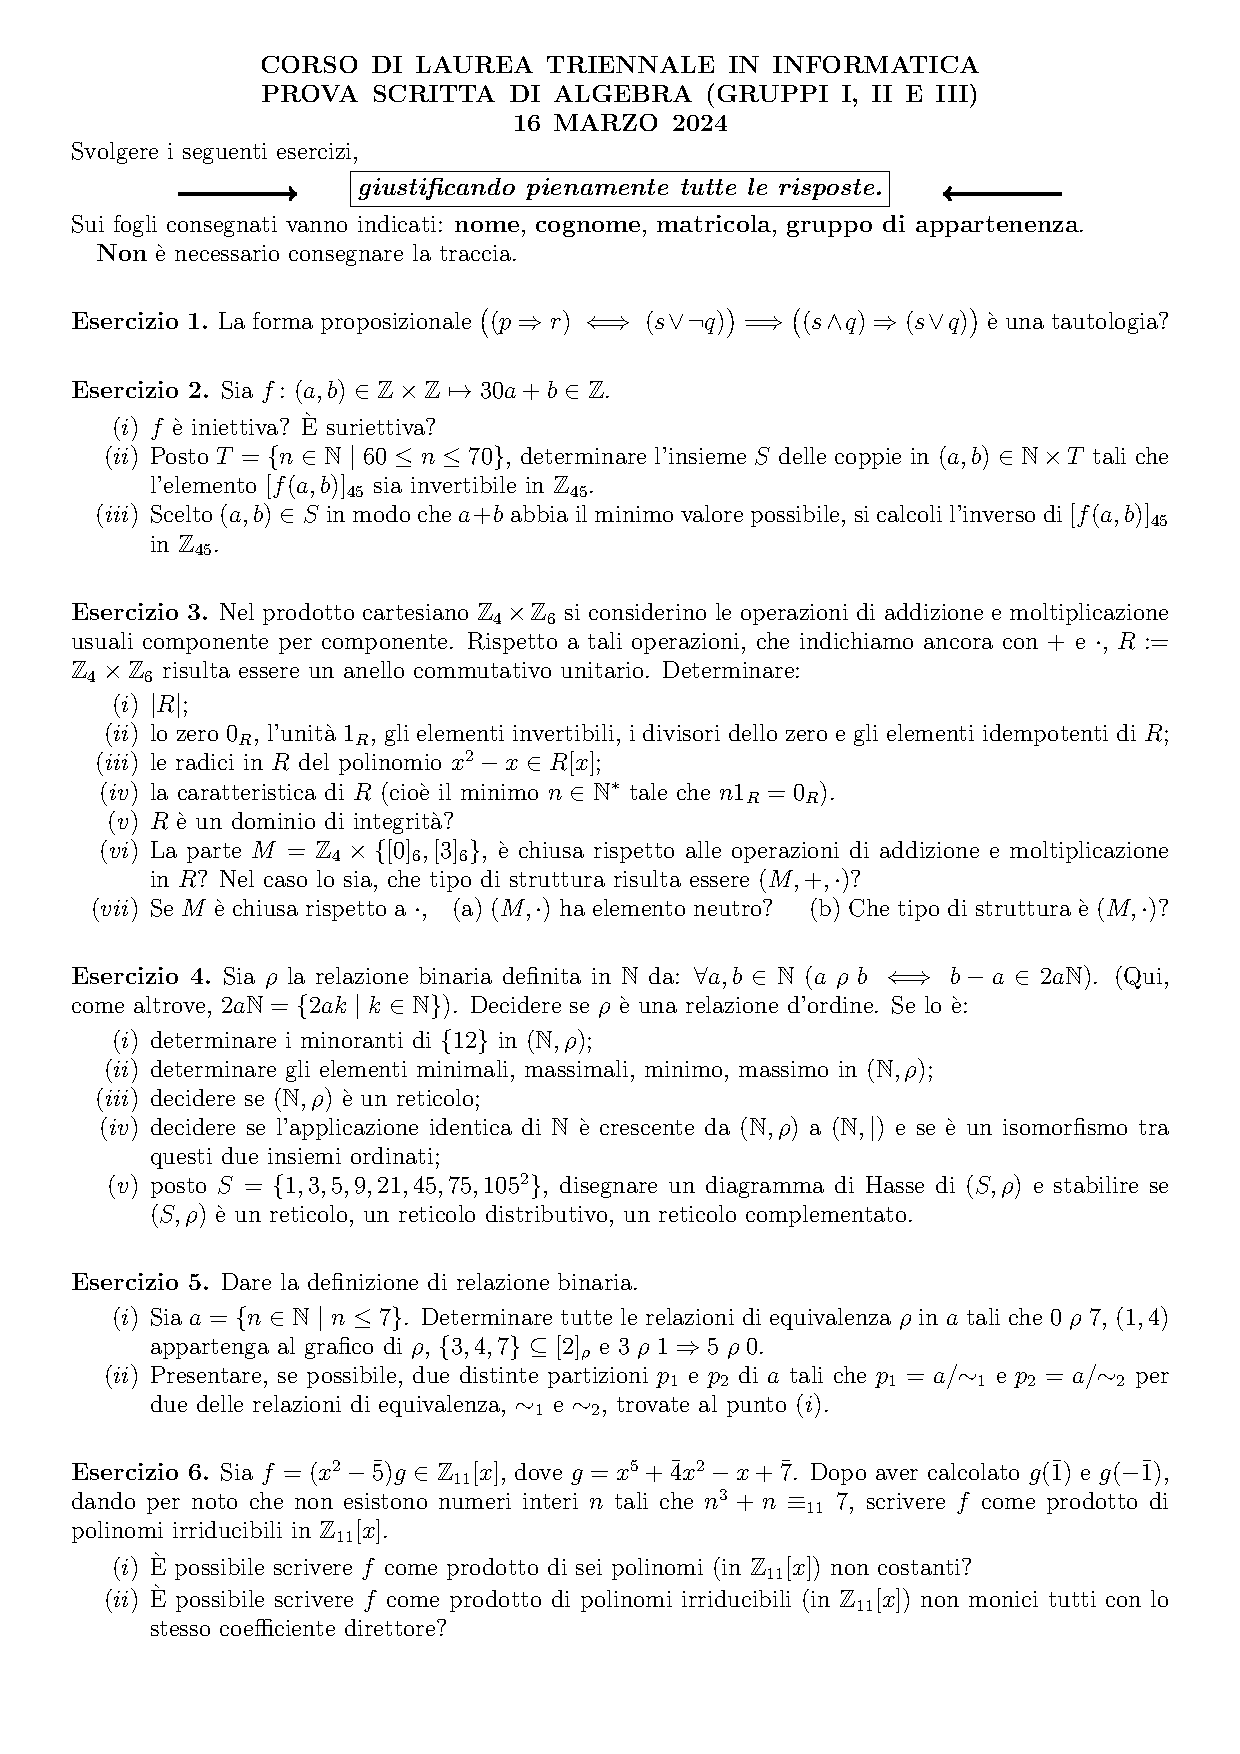
\includegraphics[scale=.85]{pdf/24-03-16.pdf}
\end{center}
\subsection*{Esercizio 1}
Poniamo:
\begin{align*}
	\alpha &\coloneqq (p \implies r) \iff(s \lor \neg q) \\
	\beta &\coloneqq (s \land q) \implies (s \lor q)
\end{align*} 
Per verificare allora che $\alpha \implies \beta$ sia una tautologia proviamo che questa non può risultare mai falsa. Per risultare falsa deve essere vera $\alpha$ e falsa $\beta$. Se $\beta$ risultasse falsa avremmo che $(s \land q)$ debba risultare vera mentre $(s \lor q)$ falsa. Però, se $(s \land q)$ è vera, lo saranno sia $s$ che $q$, quindi $(s \lor q)$ in particolare non potrebbe risultare falsa. Da questo controsenso possiamo concludere che $\alpha \implies \beta$ è una tautologia. \hfill \blacksquare
\subsection*{Esercizio 2}
\begin{enumerate}[label=(\textit{\roman*})]
	\item La funzione non è iniettiva. Infatti prese le coppie $(1,0)$ e $(-1,60)$ otteniamo:
	\begin{displaymath}
		f((1,0)) = 30 \cdot 1 + 0 = 30 = 30 \cdot -1 + 60 = f((-1,60))
	\end{displaymath}
	\item La funzione è suriettiva, infatti per ogni $z \in \mathbb{Z}$ abbiamo che $z = f(0,z)$. Quindi, per ogni numero intero $z \in \mathbb{Z}$ esiste una coppia $(a,b) \in \mathbb{Z} \times \mathbb{Z}$ tale che $f((a,b))=z$.
	\item Un elemento $[f(a,b)]_{45} \in \mathbb{Z}_{45}$ risulta essere invertibile se e solo se $MCD(f(a,b),45)=1$. Ovvero se non esiste alcun divisore comune diverso da 1 tra di loro.
	
	Per avere che un numero intero della forma $30a+b$ sia coprimo con 45 sarà necessario assicurarsi che questo non condivida alcun fattore primo con $45$, cioè non essere divisibile né per 3 né per 5, in quanto $45=3^{2}\cdot 5$. Essendo $30=3 \cdot 5 \cdot 2$, un intero della forma $30a$ avrà sempre divisori in comune con $45$, quindi sarà sufficiente imporre a $b$ di non annullare i contributi di $3$ e $5$ in $a$. Ovvero imponendo che $b$ non sia divisibile per $3$ e $5$.
	
	Possiamo quindi descrivere $S$ come l'insieme delle coppie $(a,b)$ con $a \in \mathbb{N}$ e $b \in \{61,62,64,67,68\}$.
	\item Presa la coppia $(0,61)$ procediamo a calcolare l'inverso di $[61]_{45}=[16]_{45}$. Cerchiamo dunque un elemento $x \in \mathbb{Z}_{45}$ tale che $16x \equiv_{45} 1$. Procediamo utilizzando l'algoritmo delle divisioni successive:
	\begin{align*}
		45 &= 16 \cdot 2 + 13 \\
		16 &= 13 \cdot 1 + 3 \\
		13 &= 3 \cdot 4 + 1 \\
		3 &= 1 \cdot 3 + 0
	\end{align*}
Si ottiene quindi:
\begin{align*}
	1 &= 13 +(-4)3 \\
	&= (45 +(-2)16) + (-4)(16+(-1)13) \\
	&= 45 + (-6)16 +(4)45 + (-8)16 \\
	&= (5)45+(-14)16
\end{align*}
Da cui possiamo vedere che $x=[-14]_{45}=[31]_{45}$ è la soluzione cercata. 

\end{enumerate}
\subsection*{Esercizio 3}
\begin{enumerate}[label=(\textit{\roman*})]
	\item $|R| = |\mathbb{Z}_{4}| \times |\mathbb{Z}_{6}| = 4 \cdot 6 = 24$.
	\item Si ha $0_{R}=(0,0)$ e $1_{R}=(1,1)$. Infatti, per ogni coppia $(a,b) \in R$ si ha:
	\begin{align*}
		(a,b)+(0,0) =(a+0,b+0)=(a,b) \\
		(a,b)\cdot(1,1)=(1\cdot a, 1 \cdot b) = (a,b)
	\end{align*}
	Un elemento $(a,b) \in R$ è invertibile se esiste un elemento $(a',b')$ tale che:
	\begin{displaymath}
		(a,b) \cdot (a',b') = (a \cdot a', b \cdot b') = (1,1)
	\end{displaymath}
	La ricerca di tali coppie in $R$ può essere ridotta quindi alla ricerca degli elementi invertibili in $\mathbb{Z}_{4}$ e $\mathbb{Z}_{6}$. Per la Proposizione \ref{prop:invertibili_zm} sappiamo che in $\mathbb{Z}_{4}$ risultano essere invertibili gli elementi $\overline{1}$ e $\overline{3}$ mentre in $\mathbb{Z}_{6}$ sono invertibili gli elementi $\overline{5}$ e $\overline{1}$. Otteniamo così le seguenti 4 coppie di elementi invertibili:
	\begin{displaymath}
		\mathcal{U}(R,\cdot) =\{(1,1),(1,5),(3,1),(3,5)\}
	\end{displaymath}
	Facendo un ragionamento analogo otteniamo che in $\mathbb{Z}_{4}$ risultano essere divisori dello zero gli elementi $\overline{0}$ e $\overline{2}$ mentre sono divisori dello zero in $\mathbb{Z}_{6}$ gli elementi $\overline{0},\ \overline{2}, \ \overline{3}, \ \overline{4}$. Le coppie di $R$ che risultano essere divisori dello zero sono quindi:
	\begin{displaymath}
		\{(0,0),(0,2),(0,3),(0,4),(2,0),(2,2),(2,3),(2,4)\}
	\end{displaymath}
	Un elemento $(a,b) \in R$ è idempotente se, e soltanto se, $(a,b) \cdot (a,b) = (a,b)$. In altre parole deve essere:
	\begin{displaymath}
		\begin{cases}
			a^{2} \equiv_{4} a \\
			b^{2} \equiv_{6} b
		\end{cases}
	\end{displaymath}
	L'equazione $a^{2} \equiv a (mod 4)$ è equivalente all'equazione $a^{2} \equiv a (mod 2)$ che è sua volta equivalente a $a(a-1) \equiv 0 (mod 2)$ che ha soluzioni solo per $a=0, \ a= 1$ per la legge di annullamento del prodotto. Seguendo un ragionamento analogo, l'equazione $b^{2}\equiv b (mod 6)$ è risolta da $b \in \{0,1,3,4\}$. Otteniamo quindi che le coppie:$$(0,0), \ (0,1),\ (0,3),\ (0,4),\ (1,0),\ (1,1),\ (1,3), \ (1,4)$$ risultano essere idempotenti in $R$.
	\item Un elemento di $R$ è radice del polinomio $x^{2}-x$ se e soltanto se:
	\begin{align*}
		(a,b)\cdot (a,b) - (a,b) = (0,0) &\iff (a^{2}-a,b^{b}-b) = (0,0) \\
		&\iff \begin{cases*}
			a^{2} = a \\
			b^{2} = b
		\end{cases*}
	\end{align*}
Quindi tutte le coppie di elementi idempotenti in $R$ trovate nel punto precedente sono radici di tale polinomio.
	\item Risulta $mcm(4,6)=12$ e vale $12 \cdot 1_{R}=12 \cdot (1,1)=(12,12)=(0,0)=0_{R}$, quindi la caratteristica di $R$ è 12.
	\item $R$ non è un dominio di integrità in quanto sono presenti divisori dello zero.
	\item Siano $(a,b),(c,d) \in M$ e consideriamo le composte $(a,b)+(c,d) =(a+c,b+d)$ e $(a,b)\cdot(c,d)=(ac,bd)$. Per verificare la stabilità di $M$ deve essere $b+d \in \{[0]_{6},[3]_{6}\}$ e $bd \in \{[0]_{6},[3]_{6}\}$, che risulta banalmente vero. $(M,+,\cdot)$ risulta quindi essere un anello commutativo. 
	\item $(M,+,\cdot)$ è un anello unitario in quanto la coppia $(1,3) \in M$ risulta essere un elemento neutro rispetto alla moltiplicazione, quindi $(M,\cdot)$ è un monoide.
\end{enumerate}
\subsection*{Esercizio 4}
La relazione $\rho$ è una relazione d'ordine. Infatti:
\begin{itemize}
	\item È \textit{riflessiva}: $\forall a \in \mathbb{N} \bigl( a \ \rho \ a \iff (a-a)=0=2a\cdot 0 \in 2a\mathbb{N}\bigr)$;
	\item È \textit{antisimmetrica}: siano $a,b \in \mathbb{N}$ tali che $a \ \rho \ b$ e $b \ \rho \ b$. Allora vale, per opportuni $k,m \in \mathbb{N}$:
	\begin{align*}
		\begin{cases}
			b-a &= 2ak \\
		a-b &= 2bm
		\end{cases}
	\implies 
	\begin{cases}
		b = 2ak+a = a(2k+1)\\
		a = 2bm+b = b(2m+1)
	\end{cases}
	\end{align*}
Sostituendo la seconda equazione nella prima si ottiene:
\begin{align*}
	a = \bigl(a (2m+1)(2k+1)\bigr)
\end{align*}
Per cui deve essere $(2m+1)(2k+1)=1$ che risulta vera se e solo se $m=k=0$, allora sostituendo tali valori nelle prime equazioni si ottiene $b-a=0 \iff b=a$.
\item È \textit{transitiva:} siano $a,b,c \in \mathbb{N}$ tali che $a \ \rho \ b$ e $b \ \rho \ c$. Quindi $b-a \in 2a\mathbb{N}$ e $c-b \in 2b\mathbb{N}$. Dimostriamo che $c-a \in 2a\mathbb{N}$. Ripetendo un ragionamento analogo a quanto visto per dimostrare l'antisimmetria della relazione $\rho$, abbiamo che $b = a(2k+1)$ e $c=b(2m+1)$ per un opportuni $k,m \in \mathbb{N}$. Sostituendo l'equazione di $b$ nella seconda si ottiene:
\begin{align*}
	c&=b(2m+1) \\
	&=\bigl(a(2k+1)\bigr)(2m+1)
\end{align*}
Calcoliamo quindi la differenza $c-a$:
\begin{align*}
	c-a &= \bigl(a(2k+1)\bigr)(2m+1) -a \\
	&= a \bigl((2k+1)(2m+1)-1\bigr) \\
	&= a \bigl(4km + 2k +2m + 1 -1\bigr) \\
	&= a \bigl(2(km+k+m)\bigr) \\
	&= a \cdot 2 \nu \in 2a \mathbb{N} & \text{\textcolor{gray}{(Ponendo $km+k+m = \nu $)}}
\end{align*}
Il che dimostra la transitività della relazione $\rho$.
\end{itemize}
\begin{enumerate}[label=(\textit{\roman*})]
	\item L'insieme dei minoranti di $\{12\}$ è definito come:
	\begin{displaymath}
		\{12\}^{\downarrow} = \{ n \in \mathbb{N} \; | \; n \ \rho \ 12 \}
	\end{displaymath}
	Un naturale $n \in \mathbb{N}$ ``precede'' $12$ se e solo se:
	\begin{align*}
		n \ \rho \ 12 &\iff 12 -n  \in 2n\mathbb{N} \\
		&\iff \exists k \in \mathbb{N} \bigl(12 -n = 2nk\bigr)\\
		&\iff \exists k \in \mathbb{N} \bigl(12 = n +2nk\bigr)\\
		&\iff \exists k \in \mathbb{N} \bigl(12 = n(2k+1)\bigr)\\
	\end{align*}
Quindi se, e solo se $n \divides 12$ e $12/n$ è dispari. I divisori di 12 sono $\{1,2,3,4,6,12\}$, eseguendo dei rapidi calcoli otteniamo che per $n=4$ si ottiene $12/4=3$ e per $n=12$ si ha $12/12=1$. Quindi:
\begin{displaymath}
	\{12\}^{\downarrow} = \{4,12\}
\end{displaymath}
\item Un elemento $a \in \mathbb{N}$ è minimale se e solo se non esiste un naturale $b \in \mathbb{N}$ tale che sia $b \neq a$ e $b \ \rho \ a$. Ossia:
\begin{align*}
	a \ \text{minimale in $\mathbb{N}$} &\iff \neg \bigl(\exists b \in \mathbb{N}( b \ \rho \ a \land b \neq a)\bigr) \\
	&\iff \neg \bigl(\exists b \in \mathbb{N}( a-b \in 2b\mathbb{N} \land b \neq a)\bigr) \\ 
	&\iff \neg \bigl(\exists b \in \mathbb{N}( b \divides a \land \exists k \in \mathbb{N}(\frac{a}{b} = (2k+1)) \land b \neq a)\bigr) \\
\end{align*}
Chiaramente $1$ risulta minimale in $\mathbb{N}$, così come il 2. Ogni numero dispari è preceduto da almeno $1$ e non può appartenere quindi all'insieme dei minimali. Infatti, preso un numero dispari della forma $m= (2k+1)$ abbiamo che $1 \divides m$ e $\frac{m}{1} = 2k+1$. Restano da analizzare quindi solo i numeri pari, ovvero gli elementi dell'insieme $2\mathbb{N}=\{2t \; | \; t \in \mathbb{N} \}$. Se $t$ è dispari abbiamo che il numero $n = 2t$ può essere scritto come $2 \cdot (2k+1)$ ed è chiaro che $(2k+1) \ \rho \ n$. Sia $t$ pari, in questo caso $n$ risulta essere una potenza del 2 che può essere scritta come $2^{k}$. Gli unici divisori propri di $2^{k}$ saranno le potenze del tipo $2^{j}$ con $j < k$ e $\frac{2^{k}}{2^{j}}=2^{k-j}$ che risulta essere pari. Possiamo affermare quindi che, se $n$ è una potenza del due, non esistono naturali $m$, diversi da $n$ stesso, che dividano $n$ e tali che $\frac{n}{m}$ sia dispari. Quindi l'insieme elementi minimali di $(\mathbb{N},\rho)$ è rappresentato da tutte le potenze del 2. Avendo infiniti minimali non esiste il minimo in $(\mathbb{N},\rho)$. 

Dato che ogni numero è ``coperto'' da un suo multiplo, non esistono elementi massimali in $\mathbb{N}$, e di conseguenza neanche massimi.
\item Considerata una qualsiasi coppia di elementi $\{2^{i},2^{j}\}$ con $i,j \in \mathbb{N}$ osserviamo che non esiste estremo inferiore in $(\mathbb{N},\rho)$ il quale non risulta essere quindi un reticolo.
\item Sia $f: (\mathbb{N},\rho) \rightarrow (\mathbb{N},\divides)$ l'applicazione identica. Chiaramente questa risulta crescente per come è definita la relazione $\rho$. Infatti, presi $a, b \in \mathbb{N}$:
\begin{align*}
	a \ \rho \ b &\iff b-a \in 2a\mathbb{N} \\
	&\iff \exists k \in \mathbb{N} \bigl( b= 2ak+a\bigr) \\
	&\iff \exists k \in \mathbb{N} \bigl(b=a(2k+1)\bigr) \\
	&\iff a \divides b\\
	&\iff f(a) \divides f(b)
\end{align*}
L'applicazione identica è biettiva, crescente, ma non lo è l'applicazione inversa $f^{-1}$. Infatti, presi due elementi $a,b \in \mathbb{N}$ tali che $a \divides b$, non è detto che $b$ sia esprimibile necessariamente come prodotto di $a$ per un numero dispari, condizione necessaria affinché $a \ \rho \ b$. Ad esempio presa la coppia $(4,8)$ vale $4 \divides 8$ eppure $ 4 \ \cancel{\rho} \ 8$ in quanto $8-4 \notin 2 \cdot 4 \mathbb{N} = 8\mathbb{N}$. Quindi $f$ non risulta essere un isomorfismo.
\item Si ha:
\begin{center}
	\begin{tikzpicture}
		\filldraw[black] (0,0) circle(2pt) node[anchor=north]{1};
		\filldraw[black] (0,1) circle(2pt) node[anchor=east]{3};
		\filldraw[black] (1,1) circle(2pt) node[anchor=north]{5};
		\filldraw[black] (0,2) circle(2pt) node[anchor=east]{9};
		\filldraw[black] (-1,2) circle(2pt) node[anchor=east]{21};
		\filldraw[black] (1,3) circle(2pt) node[anchor=north]{45};
		\filldraw[black] (2,3) circle(2pt) node[anchor=north]{75};
		\filldraw[black] (1,5) circle(2pt) node[anchor=south]{$105^{2}$};
		\draw[black](0,0)--(0,1);
		\draw[black](0,0)--(1,1);
		\draw[black](0,1)--(0,2);
		\draw[black](0,1)--(2,3);
		\draw[black](0,2)--(1,3);
		\draw[black](0,1)--(-1,2);
		\draw[black](-1,2)--(1,5);
		\draw[black](1,3)--(1,5);
		\draw[black](1,1)--(1,3);
		\draw[black](1,1)--(2,3);
		\draw[black](2,3)--(1,5);
	\end{tikzpicture}
\end{center}
$(S,\rho)$ è un reticolo.
\end{enumerate}
\subsection*{Esercizio 5}
Una relazione binaria è una terna $\rho = (A,A,G)$ dove $A$ è un insieme e $G\subseteq A\times A$.
\begin{enumerate}[label=(\textit{\roman*})]
	\item Preso $a=\{1,2,3,4,5,6,7\}$ consideriamo tutte le relazioni $\sim=(A,A,G)$ dove:
	\begin{align*}
		\{(0,7),(1,4),(2,3),(2,4),(2,7)\} \subseteq G
	\end{align*}
	Inoltre, se la coppia $(3,1)$ appartiene al grafico allora anche la coppia $(5,0) \in G$. Per la proprietà transitiva sappiamo che $(1 \sim 4) \land (4  \sim  2)$, quindi $(1,2) \in G$. Analogamente, da $(0  \sim  7) \land (7 \sim 2)\implies (0 \sim 2)$. Infine, essendo $(3 \sim  2) \land (2 \sim 0) \implies (3 \sim 0) \implies (5 \sim 0)$. La parte $[2]_{\sim}=\{0,1,2,3,4,5,7\}$ risulta quindi un'unica classe di equivalenza, dalla quale resta escluso l'elemento 6. Possiamo considerare quindi due casi, e di conseguenza due relazioni di equivalenza: 
	\begin{enumerate}
		\item Se 6 è in relazione con un elemento di $[2]_{\sim}$ allora $\sim_{1} = \tau_{A}$ è la relazione totale.
		\item Se 6 non è in relazione con alcun elemento di $[2]_{\sim}$ allora sarà in relazione $\sim_{2}$ solo con sè stesso.
	\end{enumerate}
	
	\item Per il Teorema \ref{thm:equivalenza_partizione} esiste una applicazione biunivoca tra l'insieme $Eq(a)$ e $Partz(a)$. Si ottengono le due partizioni:
	\begin{itemize}
		\item $A/\{\sim_{1}\}=A/\{\tau_{A}\}=\{A\}$
		\item $A/{\sim_{2}}=\{[2]_{\sim},[6]_{\sim}\}$ dove $[6]_{\sim}=\{6\}$.
	\end{itemize}
\end{enumerate}
\begin{center}
	\begin{tikzpicture}[scale=1.5]
		
		% Coordinate for the elements
		\coordinate (A1) at (0, 0);
		\coordinate (A2) at (1, 0);
		\coordinate (A3) at (2, 0);
		\coordinate (A4) at (3, 0);
		\coordinate (A5) at (1, 1);
		\coordinate (A6) at (2, 2);
		\coordinate (A7) at (3, 1);
		
		% Draw elements
		\foreach \i/\j in {1/A1, 2/A2, 3/A3, 4/A4, 5/A5, 6/A6, 7/A7} {
			\draw[fill=white] (\j) circle [radius=0.2];
			\node at (\j) {\i};
		}
		
		% Highlight the subset {1,2,3,4,5,7}
		\draw[rounded corners=8pt, thick, dashed, red] 
		($(A1)+(-0.4,-0.4)$) rectangle ($(A7)+(0.4,0.4)$);
		\node[shape=circle,draw=blue, minimum width=1.5cm, dashed, fit={(A6)}]{};
		\node[shape=circle,draw,minimum width=8cm,fit={(A1)(A2)(A3)(A4)(A5)(A6)}]{};
	\end{tikzpicture}
	\captionof{figure}{Partizione determinata dalla relazione $\sim_{2}$}\label{fig:15324_4}
\end{center}
\subsection*{Esercizio 6}
Partiamo con l'osservare che $(\mathbb{Z}_{11}[x])$ è un campo. Il polinomio $(x^{2}-5)$ può essere scritto come:
\begin{align*}
	(x^{2}-5) = (x+4)(x-4) = (x-7)(x+7)
\end{align*} 
In quanto $4^{2} = \overline{16}_{11} = \overline{5}_{11}$ e anche $\overline{7}^{2} = \overline{49}_{11} = \overline{5}_{11}$.
Procediamo ora a calcolare $g(1)$ e $g(-1)$:
\begin{align*}
	g(1)&=(\overline{1})^{5}+4(\overline{1})^{2}-\overline{1}+\overline{7}=\overline{11}=\overline{0} \\
	g(-1) &= (\overline{-1})^{5} + 4(\overline{-1})^{2} + \overline{1} +\overline{7} = \overline{11} = 0
\end{align*}
Quindi $(x-1) \divides_{\mathbb{Z}_{11}} g$ e $(x+1) \divides_{\mathbb{Z}_{11}} g$. Procediamo quindi a fattorizzare il polinomio $g$ eseguendo la divisione lunga:
\begin{center}
	\polylongdiv[style=D]{x^{5}+4x^{2}-x+7}{x-1}
\end{center}
Dato che $\overline{11}=\overline{0}$ abbiamo ottenuto un divisore $g_{1}=x^{4}+x^{3}+x^{2}+5x+4$ che sarà divisibile per $x=-1$. Infatti, essendo $g(x) =g_{1} \cdot (x-1)$, deve valere:
\begin{align*}
	g(-1) &= g_{1}(-1) \cdot (-1 - 1) \\
	&= g_{1}(-1) \cdot (-2) = \overline{0}	\\
	&\iff g_{1}(-1) = 0 \\
	&\iff (x+1) \divides_{\mathbb{Z}_{11}} g_{1}
\end{align*}
Possiamo quindi eseguire la divisione:
\begin{center}
	\polylongdiv[style=D]{x^{4}+x^{3}+x^{2}+5x+4}{x+1}
\end{center}
Verifichiamo che $g_{3}$ sia irriducibile. Se non lo fosse dovrebbe esistere una $x \in \mathbb{Z}_{11}$ tale che $x^{3}+x+4\equiv_{11} 0$, in particolare deve essere $x^{3}+x=7$, il quale sommato a $4$, annullerebbe il polinomio. Dato che non esiste un intero $n \in \mathbb{Z}$ tale che $n^{3}+n \equiv_{11} 7$, abbiamo che $g_{2} = x^{3}+x+4$ è irriducibile. Otteniamo quindi la fattorizzazione:
\begin{align*}
	f = (x+4)(x-4)(x^{3}+x+4)(x+1)(x-1)
\end{align*}
\begin{enumerate}[label=(\textit{\roman*})]
	\item Il polinomio $f$ non è esprimibile come prodotto di sei polinomi non costanti.
	\item Il polinomio $f$ non è esprimibile come prodotto di polinomi irriducibili non monici con tutti lo stesso coefficiente direttore in quanto qualsiasi coefficiente $a \neq 1$, moltiplicato ai fattori di $f$, restituirebbe un polinomio $a \cdot f$ diverso da $f$ stesso.
\end{enumerate}
\vfill

\section{Esame del 22 aprile 2024}
\begin{center}
	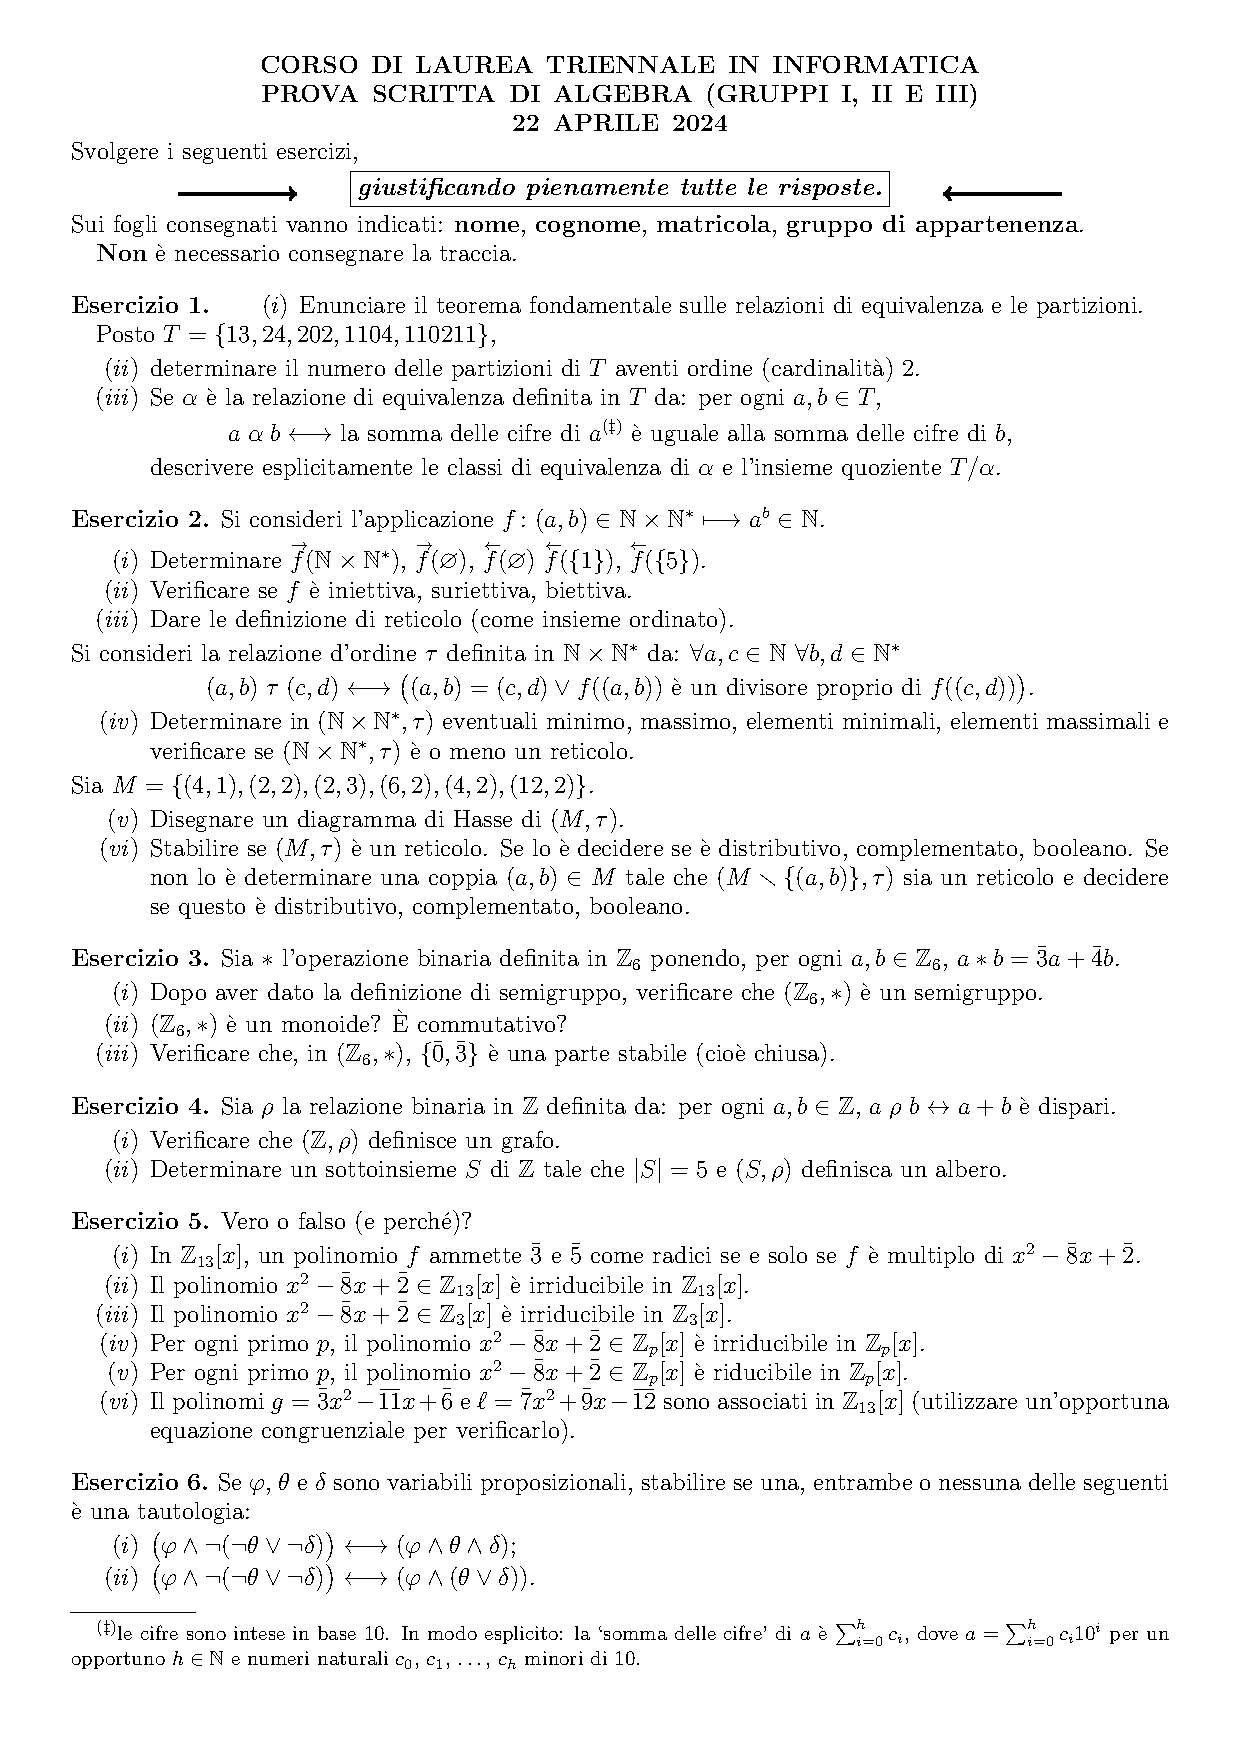
\includegraphics[scale=.85]{pdf/24-04-22.pdf}
\end{center}
\subsection*{Esercizio 1}
\begin{enumerate}[label=(\textit{\roman*})]
	\item Il Teorema fondamentale su partizioni e relazioni di equivalenza afferma che esiste una corrispondenza biunivoca tra l'insieme delle partizioni di un insieme $A$ e l'insieme delle equivalenze $Eq(A)$, cioè ogni partizione è un insieme quoziente e viceversa.
	\item Un insieme $\mathcal{F}$ per essere una partizione con due elementi deve essere costituita da due parti disgiunte di $T$, $F_{3}$ e $F_{2}$, tali che $|F_{1}|=3$ e $|F_{2}|=2$, oppure da $F_{1}$ ed $F_{4}$ con $|F_{1}|=1$ ed $|F_{4}|=4$. Il numero di parti di $T$ con tre elementi è dato da:
	\begin{align*}
		\binom{5}{3} = \frac{5!}{3!2!} = 10
	\end{align*}
Fissati tre elementi di $T$ a costituire una parte restano solo due elementi ``liberi'' per poter costituire $F_{2}$, esistono quindi $10 \cdot 1$ possibili combinazioni tra $F_{2}$ ed $F_{3}$ per costruire una partizione di $T$ con cardinalità 2. Il numero di parti con 4 elementi è invece dato da:
\begin{align*}
	\binom{5}{4} = \frac{5!}{4!}= 5
\end{align*}
Fissati quattro elementi di $T$ a costituire una parte $F_{4}$ resta una sola opzione per costruire una parte di un singolo elemento. Quindi il numero totale di partizioni di cardinalità 2 è 15.
\item Abbiamo:
\begin{itemize}
	\item $1+3=4$
	\item $2+4=6$
	\item $2+0+2=4$
	\item $1+1+0+4=6$
	\item $1+1+0+2+1+1=6$
\end{itemize}
Quindi $T/{\alpha}=\{\{13,202\},\{24,1104,110211\}\}$.
	\end{enumerate}
\subsection*{Esercizio 2}
\begin{enumerate}[label=(\textit{\roman*})]
\item Si ha: 
\begin{itemize}
	\item $\overrightarrow{f}(\mathbb{N} \times \mathbb{N}^{*})=\mathbb{N}$
	\item $\overrightarrow{f}(\emptyset) = \emptyset$
	\item $\overleftarrow{f}(\emptyset) = \emptyset$
	\item $\overleftarrow{f}(\{1\})=\{(1,n) \; | \; n \in \mathbb{N}^{*}\}$
	\item $\overleftarrow{f}(\{5\})=\{(5,1)\}$
\end{itemize}
\item L'applicazione $f$ non è iniettiva in quanto $f((0,1))=f((0,2))=0$ ma $(0,2) \neq (0,1)$. La funzione è suriettiva in quanto per ogni $n \in \mathbb{N}$ possiamo individuare una coppia $(a,b) \in \mathbb{N} \times \mathbb{N}^{*}$ tale che $f((a,b))=n$, infatti $f((n,1))=n^{1}=n$. L'applicazione, non essendo iniettiva, non è biettiva.
\item Un insieme ordinato $(S,\leq)$ è un reticolo se, e soltanto se, per ogni parte $\{a,b\} \subseteq S$ esiste estremo inferiore ed estremo superiore.
\item Il minimo di $(\mathbb{N}\times \mathbb{N}^{*})$ è dato dalla coppia $(1,1)$ in quanto, in $\mathbb{N}$, $f((1,1))=1$ divide ogni altro naturale. Poiché non esiste alcuna coppia la cui immagine secondo $f$ sia nulla, non esiste massimo e, avendo escluso tale valore, non esistono valori massimali in quanto ogni naturale non nullo è divisore dei suoi multipli. La struttura $(\mathbb{N}\times \mathbb{N}^{*},\tau)$ non è un reticolo in quanto, prese ad esempio le coppie $\bigl\{(1,2),(2,1)\bigr\}$, abbiamo:
\begin{align*}
	\bigl\{(1,2),(2,1)\bigr\}^{\uparrow} = \{(2,2),(4,1)\}
\end{align*}
e non esiste un minimo di tale insieme, ossia non esiste un estremo superiore.
\item Essendo:
\begin{itemize}
	\item $f((4,1))=4^{1}=4$
	\item $f((2,2))=2^{2}=4$
	\item $f((2,3))=2^{3}=8$
	\item $f((6,2))=6^{2}=36$
	\item $f((4,2))=4^{2}=16$
	\item $f((12,2))=12^{2}=144$
\end{itemize} 
Abbiamo:
\begin{center}
	\begin{tikzpicture}
		\node[circle,fill=black,inner sep=0pt,minimum size=3pt,label=below:{$(4,1)$}](a) at (0,0){};
		\node[circle,fill=black,inner sep=0pt,minimum size=3pt,label=below:{$(2,2)$}](b) at (2,0){};
		\node[circle,fill=black,inner sep=0pt,minimum size=3pt,label=left:{$(2,3)$}](c) at (0,1){};
		\node[circle,fill=black,inner sep=0pt,minimum size=3pt,label=left:{$(6,2)$}](d) at (2,1){};
		\node[circle,fill=black,inner sep=0pt,minimum size=3pt,label=left:{$(4,2)$}](e) at (0,2){};
		\node[circle,fill=black,inner sep=0pt,minimum size=3pt,label=left:{$(12,2)$}](f) at (0,4){};
		\draw[black,thin] (a)--(c);
		\draw[black,thin] (b)--(c);
		\draw[black,thin] (a)--(d);
		\draw[black,thin] (b)--(d);
		\draw[black,thin] (c)--(e);
		\draw[black,thin] (d)--(f);
		\draw[black,thin] (e)--(f);
	\end{tikzpicture}
\end{center}
\item $(M,\tau)$ non è un reticolo in quanto non esiste un minimo. Eliminando la coppia $(2,2)$ otteniamo un reticolo distributivo, complementato, e quindi booleano.
\end{enumerate}

\subsection*{Esercizio 3}
\begin{enumerate}[label=(\textit{\roman*})]
	\item Un semigruppo è una struttura $(S,\bot)$ in cui $\bot$ è associativa. $(\mathbb{Z}_{6},\ast)$ è un semigruppo in quanto, per ogni terna di elementi $a,b,c \in \mathbb{Z}_{6}$ abbiamo:
	\begin{align*}
		a \ast (b \ast c) &= a \ast (3b + 4c ) \\
		&= 3a + 4(3b+4c) \\
		&= 3a + 12b + 16c \\
		&= 3a + 4c
	\end{align*}
e:
\begin{align*}
	(a \ast b) \ast c &= (3a+4b) \ast c \\
	&= 3(3a+4b)+4c \\
	&= 9a + 12b + 4c \\
	&= 3a + 4c
\end{align*}
\item L'operazione non è commutativa, presi $a=1$ e $b=0$ si ha ad esempio $a \ast b = 1 \neq 4 = b \ast a$.
\item Si ha: $0 \ast 0 = 0$, $0 \ast 3 = \overline{12}=\overline{0}$, $3 \ast 0 = \overline{9}=\overline{3}$, $3 \ast 3 = 3$. Quindi $\{0,3\}$ è stabile.
\end{enumerate}
\subsection*{Esercizio 4}
\begin{enumerate}
	\item Essendo $\rho$ una relazione binaria antiriflessiva e simmetrica la coppia $(\mathbb{Z},\rho)$ risulta essere un grafo.
	\item Un albero è un grafo connesso senza circuiti. Consideriamo l'insieme $S=\{1,2,4,10,20\}$ e l'insieme dei lati:
	\begin{align*}
		L = \{(1,2),(1,4),(1,10),(1,20)\}
	\end{align*}
Si ottiene così il seguente albero:
\begin{center}
	\begin{forest}
	for tree={circle,draw}
		[1
			[2]
			[4]
			[10]
			[20]
		]
	\end{forest}
\end{center}
\end{enumerate}

\subsection*{Esercizio 5}
\begin{enumerate}[label=(\textit{\roman*})]
	\item Siano $\overline{3}$ e $\overline{5}$ radici di $f$. Ciò significa che, per il teorema di Ruffini generalizzato, $(x-3)(x-5)$ divide $f$. Sviluppando $(x-3)(x-5)$ otteniamo il polinomio $(x^{2}-8x+2)$, quindi $f$ è un multiplo di $(x^{2}-8x+2)$. Analogamente, se $f$ è un multiplo di $(x^{2}-8x+2)$, essendo $\mathbb{Z}_{13}$, le sue radici sono tutte e sole le radici dei suoi multipli. Quindi l'equivalenza è vera.
	\item Il polinomio $(x^{2}-8x+2)$ non è irriducibile in quanto ammette due radici e può essere decomposto in $(x-3)(x-5)$;
	\item Il polinomio $(x^{2}-8x+2) \in \mathbb{Z}_{3}$ è irriducibile in quanto non ammette radici in $\mathbb{Z}_{3}$.
	\item Falso.
	\item  Falso.
	\item Vero, per trovare un fattore moltiplicativo che moltiplicato al coefficiente direttore di $g$ ci dia il coefficiente direttore di $l$ risolviamo l'equazione congruenziale $7x\equiv_{13} 3$ ottenendo $x=\overline{6}$ come risultato. Moltiplicando il polinomio $l$ per la costante $6$  otteniamo così il polinomio $g$:
	\begin{align*}
		6 \cdot (7x^{2} +9x -12) &= 42x^{2}+63x-72 \\
		&= 3x^{2}-11x+6
	\end{align*}
Saremmo potuti arrivare allo stesso risultato risolvendo l'equazione congruenziale $3x \equiv_{13} 7$ che ha per soluzione $x=11$, infatti:
\begin{align*}
	11 \cdot (3x^{2}-11x+6) &= 11 \cdot (3x^{2}+3x+6) \\
	&= 33x^{2} +22x +66 \\
	&= 7x^{2}+9x-12
\end{align*}
\end{enumerate}
\subsection*{Esercizio 6}
\begin{enumerate}[label=(\textit{\roman*})]
	\item Vero per De Morgan
	\item Falso
\end{enumerate}
\vfill

\section{Esame del 15 luglio 2024}
\begin{center}
	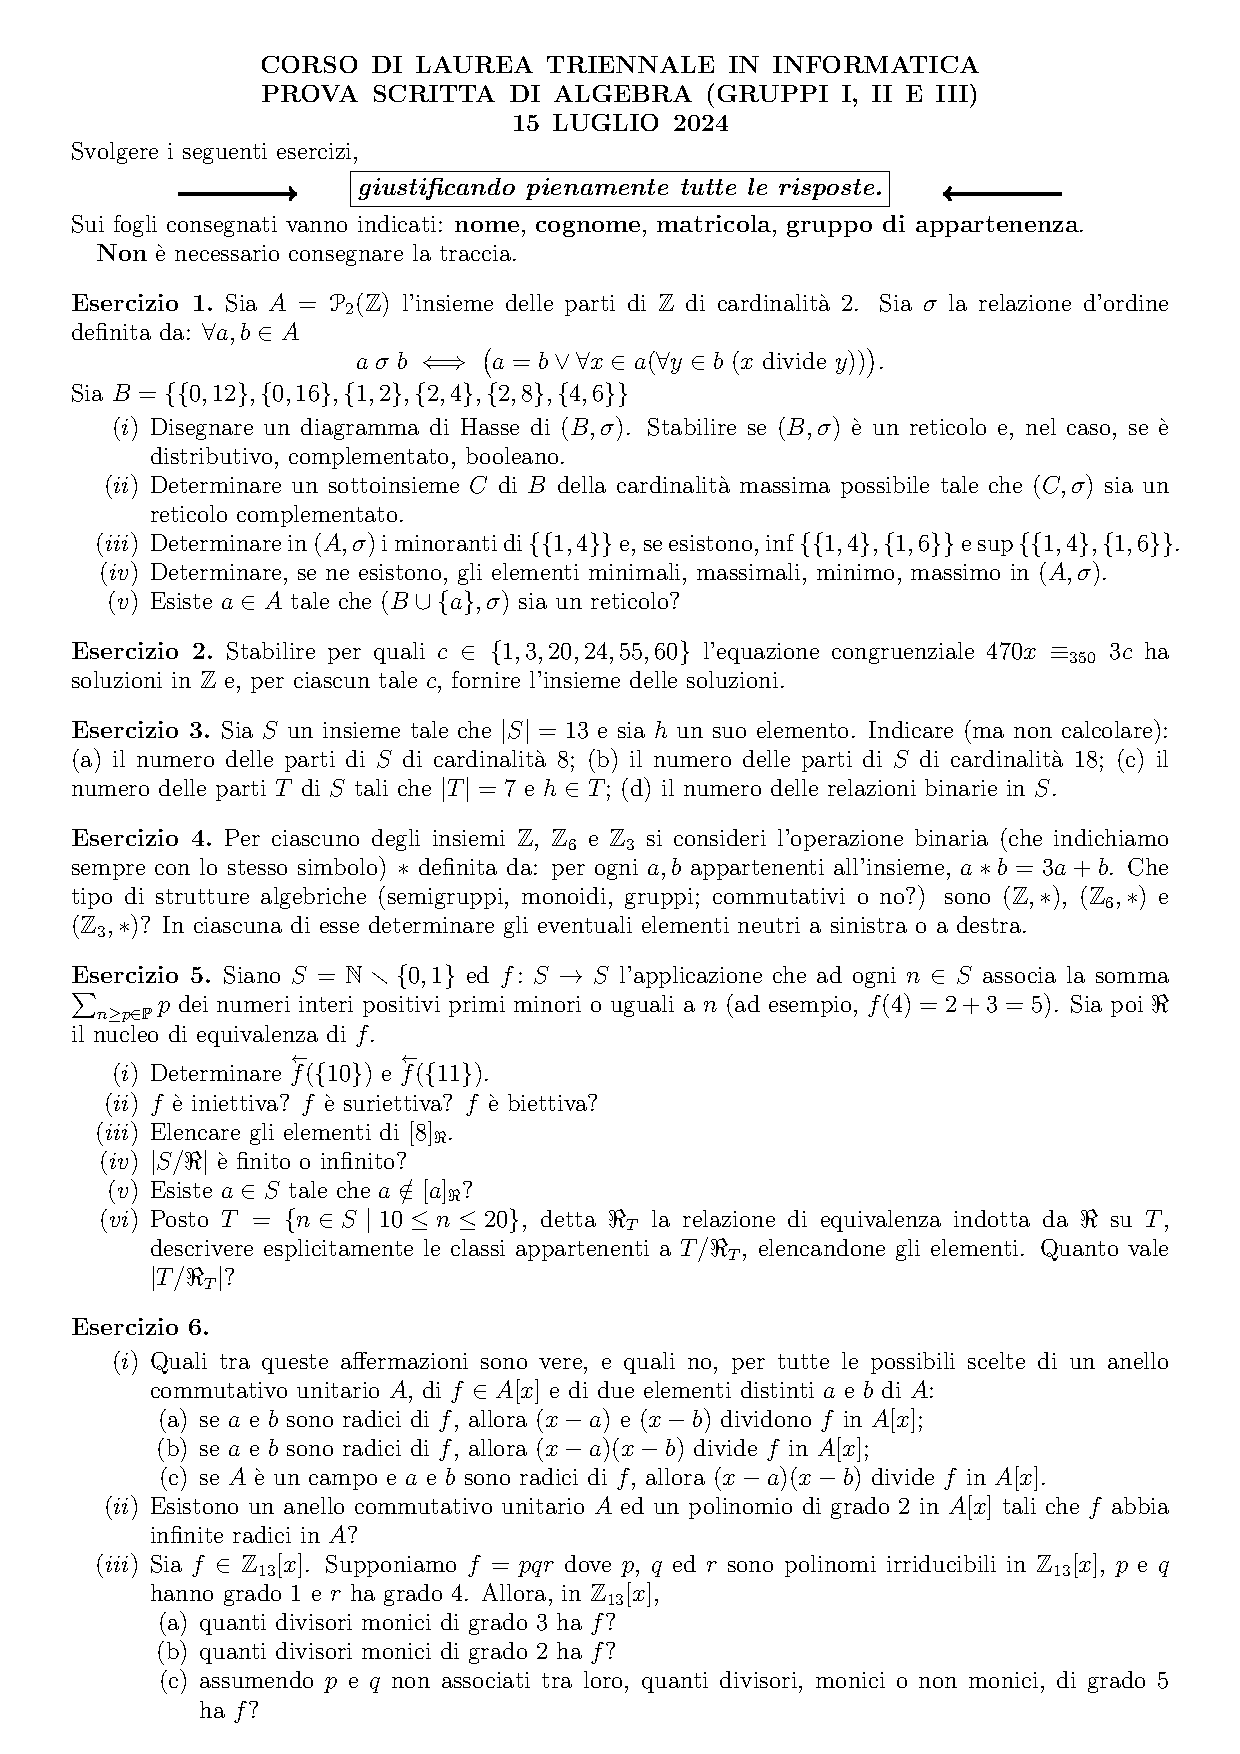
\includegraphics[scale=.85]{pdf/24-07-15.pdf}
\end{center}
\subsection*{Esercizio 1}
\begin{enumerate}[label=(\textit{\roman*})]
	\item Notiamo che $\forall x \in \mathbb{Z}(x \divides 0)$, e che $\forall x \in \mathbb{N}(1 \divides x)$. Sono inconfrontabili le parti $\{2,4\} \cancel{\sigma} \{2,8\}$ in quanto $4 \ndivides 2$; $\{2,4\} \cancel{\sigma} \{4,6\}$ poiché $4 \ndivides 6$; $\{2,8\} \cancel{\sigma} \{4,6\}$ poiché $8 \ndivides 4 \land 8 \ndivides 6$. La parte $\{1,2\}$ precede ogni altro elemento di $B$. Sono inconfrontabili le parti $\{0,12\}$ e $\{0,16\}$ in quanto $12 \ndivides 16$. Vale $\{2,4\} \sigma \{0,16\}$, $\{2,4\} \sigma \{0,12\}$, $\{4,6\} \sigma \{0,12\}$. Si ottiene così il seguente diagramma di Hasse:
	\begin{center}
		\begin{tikzpicture}
			\filldraw[black] (0,0) circle(2pt) node[anchor=north]{$\{1,2\}$};
			\filldraw[black] (-2,1) circle(2pt) node[anchor=north]{$\{2,8\}$};
			\filldraw[black] (0,1) circle(2pt) node[anchor=north]{$\{2,4\}$};
			\filldraw[black] (2,1) circle(2pt) node[anchor=north]{$\{4,6\}$};
			\filldraw[black] (-1,2) circle(2pt) node[anchor=south]{$\{0,16\}$};
			\filldraw[black] (1,2) circle(2pt) node[anchor=south]{$\{0,12\}$};
			\draw[black] (0,0)--(0,1);
			\draw[black] (0,0)--(-2,1);
			\draw[black] (0,0)--(2,1);
			\draw[black] (-2,1)--(-1,2);
			\draw[black] (2,1)--(1,2);
			\draw[black] (0,1)--(-1,2);
			\draw[black] (0,1)--(1,2);
		\end{tikzpicture}
	\end{center}
	$(S,\sigma)$ non è quindi un reticolo in quanto possiamo vedere che esistono in $(B,\sigma)$ due elementi massimali.
	\item Preso $C=\{\{1,2\},\{2,8\},\{2,4\},\{0,16\}\}$ di cardinalità 4 abbiamo che $0 = min(C,\sigma) = \{1,2\}$ e $1 = max(C,\sigma) = \{0,16\}$ e per ogni $x \in C \bigl(\exists y \in C (x \vee y = 1 \land x \wedge y = 0)\bigr)$, ovvero $(C,\sigma)$ è complementato.
	\item Abbiamo $\{\{1,4\}\}^{\downarrow} = \{\{1,-1\},\{1,4\}\}$. Inoltre: $\{1,4\} \wedge \{1,6\}=\{1,-1\}$ mentre $\{1,4\} \vee \{1,6\} = \{0,12\}$.
	\item Il minimo di $(A,\sigma)$ è rappresentato dalla parte $\{1,-1\}$. Esistono poi infiniti elementi massimali che sono le parti del tipo $\{0,a\}$, con $a \in \mathbb{Z}\setminus\{0\}$. Una parte $\{0,a\}$, infatti, non può essere seguita da alcun elemento di $A$ in quanto 0 non divide nessun elemento di $\mathbb{Z}$.
	\item Dato che una parte del tipo $a=\{0,x\}$ è massimale in $(A,\sigma)$ non è possibile inserire un elemento $a$ tale che $(B \cup \{a\},\sigma)$ possa diventare un reticolo.
\end{enumerate}
\subsection*{Esercizio 2}
Controlliamo per quali valori di $c \in \{1,3,20,24,55,60\}$ l'equazione $470x \equiv_{350} 3c$ ammette soluzioni. Chiaramente deve essere $d = MCD(470,350) \divides 3c$. Ovvero $d=10 \divides 3c$. Vera solo per $c=20$ e $c=60$. Abbiamo allora:
\begin{itemize}
	\item Sia $c=20$, allora l'equazione diventa: $470x \equiv_{350} 60$. Dividendo tutto per 10 si ottiene l'equazione equivalente $47x \equiv{35} 6$. È possibile scrivere $1=MCD(47,35)$ come combinazione lineare $1=47\cdot(3)+35\cdot(-4)$. Moltiplicando tutto per 6 abbiamo: $6=47 \cdot (18)+35 \cdot(-24)$. Quindi $x=[18]_{35}$ è una soluzione dell'equazione. Ovvero, l'insieme dei numeri interi $\{n \in \mathbb{Z} \; | \; n = 35k+18 \}$.
	\item Sia $c=60$. L'equazione diventa: $470x \equiv_{350} 180$. Dividendo per 10 otteniamo: $47x \equiv_{35} 18$. Moltiplicando nuovamente $1=47\cdot(3)+35\cdot(-4)$ per 18 si ha che $x=[54]_{35}=[19]_{35}=\{n \in \mathbb{Z} \; | \; n=35k+19 \}$.
\end{itemize}
\subsection*{Esercizio 3}
\begin{enumerate}[label=(\textit{\roman*})]
	\item Il numero di $8$-parti di $S$ è dato dal calcolo del coefficiente binomiale di 13 su 8:
	\begin{align*}
		\binom{13}{8} &= \frac{13!}{8!(13-8)!}\\
		&=\frac{13!}{8! \cdot 5!} \\
		&= \frac{13 \cdot 12 \cdot 11 \cdot 10 \cdot 9 \cdot 8 \cdot 7 \cdot 6 \cdot 5 \cdot 4 \cdot 3 \cdot 2 \cdot 1}{(8 \cdot 7 \cdot 6 \cdot 5 \cdot 4 \cdot 3 \cdot 2 \cdot 1)(5 \cdot4 \cdot 3 \cdot 2 \cdot 1)} \\
		&= \frac{13 \cdot 12 \cdot 11 \cdot 10 \cdot 9 \cdot \cancel{8 \cdot 7 \cdot 6 \cdot 5 \cdot 4 \cdot 3 \cdot 2 \cdot 1}}{(\cancel{8 \cdot 7 \cdot 6 \cdot 5 \cdot 4 \cdot 3 \cdot 2 \cdot 1})(5 \cdot4 \cdot 3 \cdot 2 \cdot 1)} = \\
		&=\frac{13 \cdot 12 \cdot 11 \cdot 10 \cdot 9}{5 \cdot4 \cdot 3 \cdot 2 \cdot 1}\\
		&=1287
	\end{align*}
	\item Non esistono parti di $S$ di cardinalità 18.
	\item Fissato $h$ in $T$ restano da essere selezionati altri 6 elementi dall'insieme $S$ che contiene ora $13-1$ elementi disponibili. Il numero di parti di $S\setminus\{h\}$ di sei elementi è dato da:
	\begin{align*}
		\binom{12}{6} = \frac{12!}{6!(6!)} = 924
	\end{align*}
	\item Una relazione binaria in $S$ è una delle qualsiasi parti di $S \times S$, che è noto avere $13^{2}$ elementi, ovvero 169 elementi.
\end{enumerate}
\subsection*{Esercizio 4}
Osserviamo che $\ast$ non è associativa in $\mathbb{Z}$. Infatti, presa la terna $(1,2,1)$ osserviamo che $(1 \ast 2) \ast 1 = 3+6+1=10$ mentre $1 \ast (2 \ast 1) = 9+6+1=16$. Possiamo quindi affermare che $(\mathbb{Z},\ast)$ è un gruppoide. Stesso discorso in $\mathbb{Z}_{6}$ in quanto:
\begin{align*}
	\forall a,b,c \in \mathbb{Z}_{6} \bigl( a \ast (b \ast c) = a \ast (3b +c) = 3a + 9b + 3c = 3a + 3b + 3c\bigr)
\end{align*}
mentre:
\begin{align*}
	\forall a,b,c \in \mathbb{Z}_{6} \bigl( (a \ast b) \ast c) = (3a+b) \ast c = 9a+3b+c = 3a+3b+c \bigr)
\end{align*}
Che in generale non coincidono. Al contrario, in $\mathbb{Z}_{3}$ abbiamo che:
\begin{align*}
	(a \ast b) \ast c = (3a+b) \ast c = b \ast c = 3b+c = c \\
	a \ast (b \ast c) = a \ast (3b+c) = a \ast c = 3a+c = c
\end{align*}
Quindi $(Z_{3},\ast)$ risulta essere un semigruppo. Verifichiamo quindi la commutatività in $\mathbb{Z}_{3}$:
\begin{align*}
	\forall a,b \in \mathbb{Z}_{3}(a \ast b \stackrel{?}{=} b \ast a)
\end{align*}
Abbiamo:
\begin{align*}
	a \ast b = 3a+b=b\\
	b \ast a = 3b+a=a
\end{align*}
Quindi $\ast$ non è commutativa. Studiamo l'eventuale esistenza di elementi neutri a sinistra o a destra. Un elemento $t$ è neutro a sinistra se:
\begin{align*}
	\forall x \in \mathbb{Z}_{3} \bigl(t \ast x \equiv_{3} x\bigr) &\iff 	\forall x \in \mathbb{Z}_{3} \bigl(3t+x \equiv_{3} x\bigr) \\
	\forall x \in \mathbb{Z}_{3} \bigl(3t \equiv_{3} 0 \bigr)
\end{align*}

Trovando quindi che tutti gli elementi di $\mathbb{Z}_{3}$ risultano essere elementi neutri a sinistra. Verifichiamo l'esistenza di elementi neutri a destra. Un elemento è neutro a destra se:
\begin{align*}
	\forall x \in \mathbb{Z}_{3} \bigl(x \ast t \equiv_{3} x\bigr) &\iff 	\forall x \in \mathbb{Z}_{3} \bigl(3x+t \equiv_{3} x\bigr) \\
	\forall x \in \mathbb{Z}_{3} \bigl(t \equiv_{3} x\bigr)
\end{align*}
Dato che $t$, per essere neutro a destra, deve coincidere con l'elemento $x$ col quale vogliamo comporlo per ottenere $x$ stesso, possiamo concludere dicendo che non esiste un elemento neutro a destra. Dato che un monoide è una struttura dotata di un elemento neutro a destra e a sinistra possiamo dire che $(\mathbb{Z}_{3},\ast)$ non è un monoide.
\subsection*{Esercizio 5}
\begin{enumerate}[label=(\textit{\roman*})]
	\item Abbiamo:
	\begin{align*}
		\overleftarrow{f}(\{10\})&=\{n \in S \; | \; f(n)=10\} \\
		&= \{n \in S \; | \; \sum_{n \geq p \in \mathbb{P}} p = 10 \} \\
		&= \{n \in S \; | \; 2+3+5=10=f(n) \} \\
		&= \{5,6\}
	\end{align*}
	Analogamente:
	\begin{align*}
		\overleftarrow{f}(\{11\})&=\{n \in S \; | \; f(n)=11\} \\
		&= \{n \in S \; | \; \sum_{n \geq p \in \mathbb{P}} p = 11 \} = \emptyset
	\end{align*}
	Infatti nella successione delle somme $f(n)$ abbiamo:
	\begin{equation}
		\Sigma_{n} = (f(n))_{n \in S} =  \{2,5,10,17,28,\ldots\} 
	\end{equation}
	Ogni termine della successione può essere ottenuto dalla formula ricorsiva $f(n) = f(n-1)+p_{n}$.
	\item Poiché $\overleftarrow{f}(\{10\})\geq 1$ possiamo dire che l'applicazione non è iniettiva. Analogamente, essendo $\overleftarrow{f}(\{11\})= \emptyset$, possiamo dire che $f$ non è suriettiva, e quindi biettiva.
	\item Si ha:
	\begin{align*}
		[8]_{\mathfrak{R}} &= \overleftarrow{f}(\{f(8)\}) = \overleftarrow{f} (\{17\}) = \{7,8,9,10\}
	\end{align*}
	\item Osserviamo che $S/{\mathfrak{R}}$ è l'insieme delle classi di equivalenza $[n]_{\mathfrak{R}}$, ovvero partizione composta dalle parti:
	\begin{align*}
		\bigl\{\overleftarrow{f}(\{f(n)\}) \; | \; n \in S \bigr\} = \bigl\{\overleftarrow{f}(\{\Sigma_{n}\}) \; | \; n \in S \bigr\}
	\end{align*}
	Dato che la successione $(\Sigma_{n})_{n \in S}$ risulta essere infinita abbiamo che $S/{\mathfrak{R}}$ è infinito.
	\item Abbiamo che $T/{\mathfrak{R}_{T}}$ è composto dalle classi:
	\begin{itemize}
		\item $[10]_{\mathfrak{R}_{T}}=\overleftarrow{f}(\{f(10)\}) = \overleftarrow{f}(\{17\}) = \{10\}$
		\item $[11]_{\mathfrak{R}_{T}}=\overleftarrow{f}(\{f(11)\}) = \overleftarrow{f}(\{28\}) = \{11,12\}$
		\item $[13]_{\mathfrak{R}_{T}}=\overleftarrow{f}(\{f(13)\}) = \overleftarrow{f}(\{41\}) = \{13,14,15,16\}$
		\item $[17]_{\mathfrak{R}_{T}}=\overleftarrow{f}(\{f(17)\}) = \overleftarrow{f}(\{58\}) = \{17,18\}$
		\item $[19]_{\mathfrak{R}_{T}}=\overleftarrow{f}(\{f(19)\}) = \overleftarrow{f}(\{77\}) = \{19,20\}$
	\end{itemize}
	E vale $|T/{\mathfrak{R}_{T}}|=5$.
\end{enumerate}
\subsection*{Esercizio 6}
\begin{enumerate}[label=(\textit{\roman*})]
	\item Si ha:
	\begin{enumerate}[label=(\arabic*)]
		\item Vero.
		\item Falso.
		\item Vero.
	\end{enumerate}
	\item Consideriamo l'anello booleano $(\mathbb{Z}_{2},+,\cdot)$. Chiaramente, essendo ogni suo elemento idempotente, il polinomio $x^{2}+x=0$ ammette infinite radici date dalla classe di equivalenza $\overline{0}_{2}$.
	\item Abbiamo:
	\begin{enumerate}
		\item $f$ non ha divisori monici di grado 3;
		\item $f$ ha un solo divisore monico di grado 2 che è il polinomio $upq$ associato al polinomio $pq$.
		\item Un divisore di grado $5$ può essere ottenuto eseguendo il prodotto tra $pr$ o $qr$. Tali polinomi avranno un polinomio monico associato. Moltiplicando un divisore monico per un elemento non nullo di $\mathbb{Z}_{13}$​ otteniamo un divisore non monico, e ci sono 12 possibili moltiplicatori (elementi di $\mathbb{Z}_{13})$. Si ottengono quindi 24 polinomi di grado 5, monici e non monici, che dividono $f$.
	\end{enumerate}
\end{enumerate}
\vfill
\section{Esame del 10 settembre 2024}
\begin{center}
	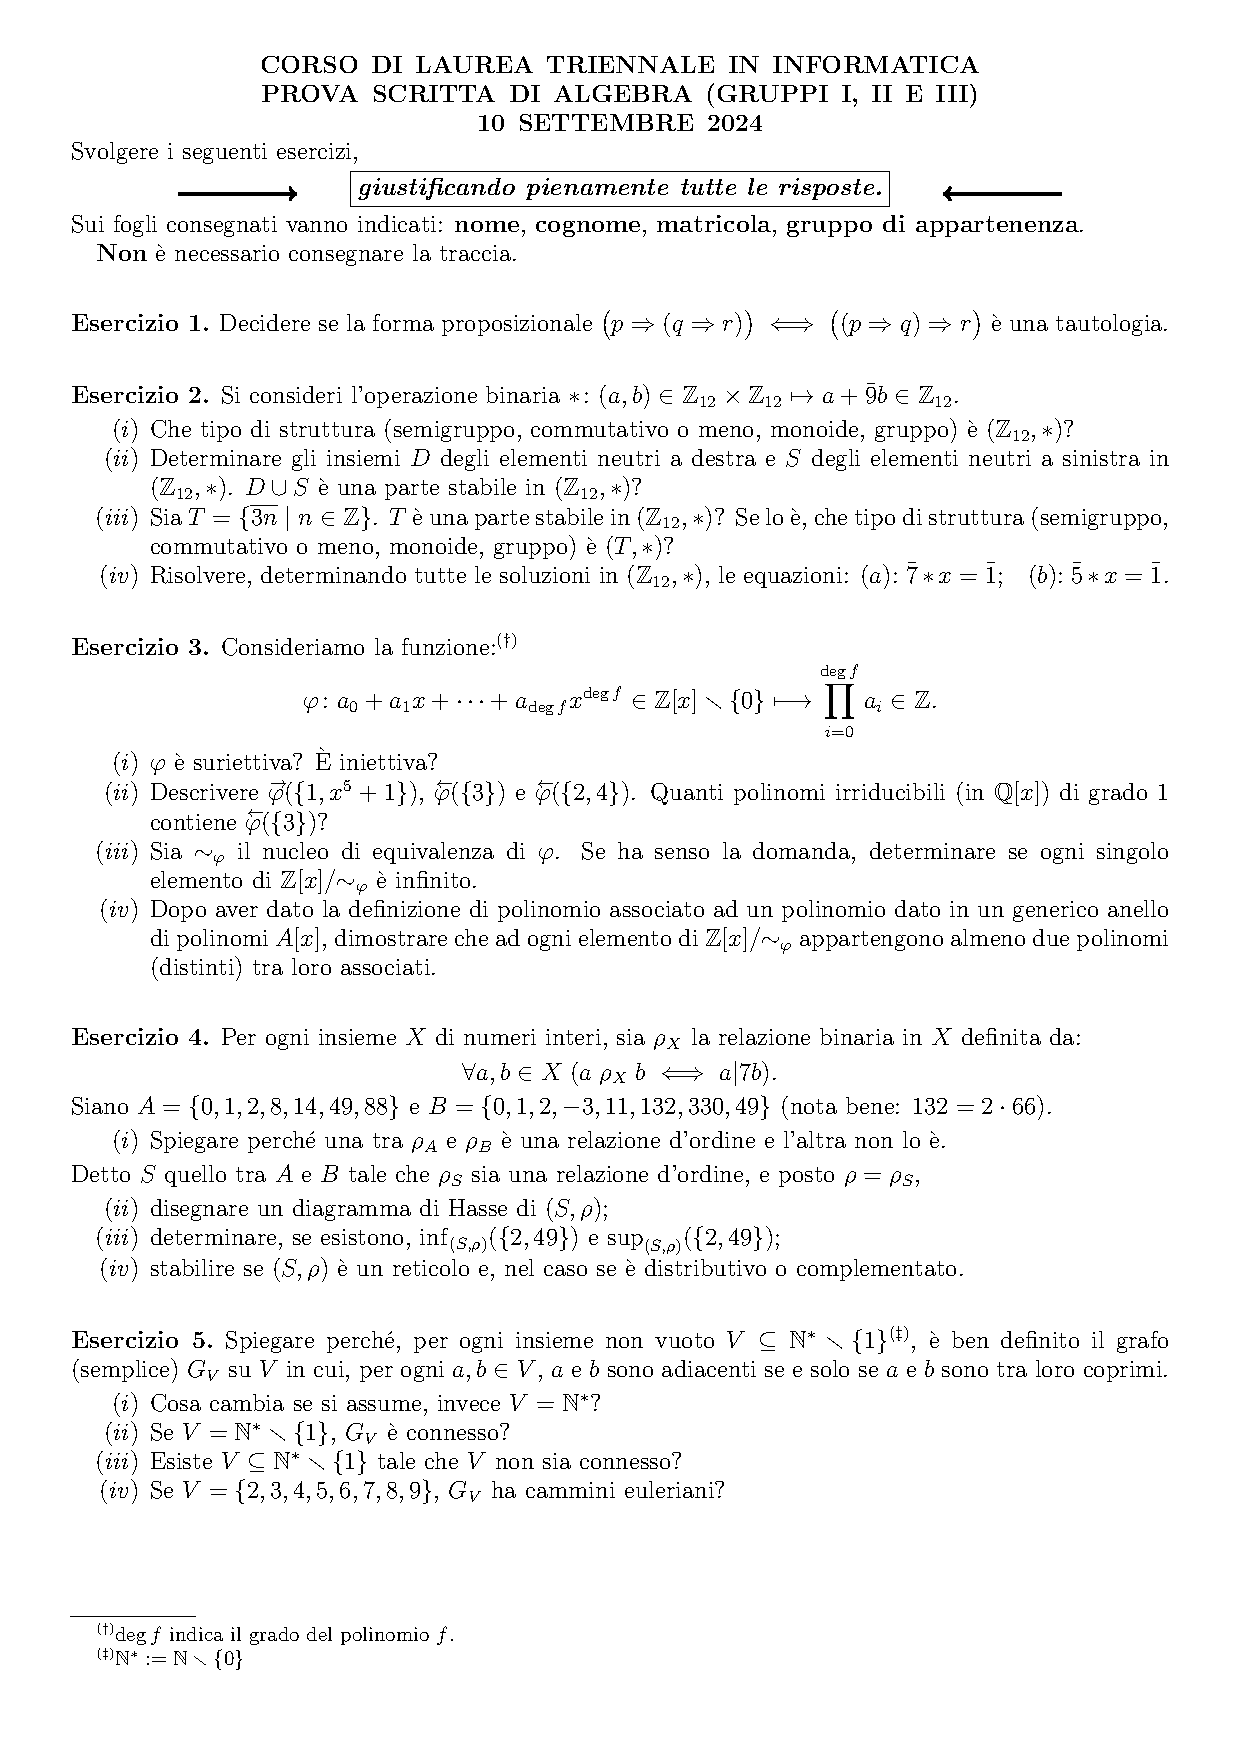
\includegraphics[scale=.85]{pdf/24-09-10.pdf}
\end{center}
\subsection*{Esercizio 1}
Costruiamo la tavola di verità:
\begin{center}
	\begin{tblr}
		{
			hlines,
			vlines,
			row{1}={primary!40!white},
			colspec={cccccX[c]X[c]},
			cells={mode=math}
		}
	p & q & r & p \implies q & q \implies r & p \implies (q \implies r) & (p \implies q) \implies r \\
	V & V & V & V & V & V & V \\
	V & V & F & V & F & F & F \\
	V & F & V & F & V & V & V \\
	V & F & F & F & V & V & V\\
	F & V & V & V & V & V & V\\
	F & V & F & V & F & V & F\\
	F & F & V & V & V & V & V\\
	F & F & F & V & V & V & F\\
	\end{tblr}
\end{center}
Le ultime due colonne non sono equivalenti e quindi possiamo affermare che non vale la proprietà associativa per l'implicazione.
\subsection*{Esercizio 2}
\begin{enumerate}[label=(\textit{\roman*})]
	\item L'operazione $\ast$ è associativa. Presi infatti tre elementi $a,b,c \in \mathbb{Z}_{12}$ abbiamo:
	\begin{align*}
		a \ast (b \ast c) &= a \ast (b+9c) \\
		&= a+ 9(b+9c) \\
		&= a+9b +81c \\
		&= a+9b+9c & \text{\textcolor{gray}{(In quanto $\overline{81}\equiv_{12} \overline{9}$)}}\\
\end{align*}
		\begin{align*}
		(a \ast b) \ast c = (a+9b) \ast c = a +9b+9c
	\end{align*}
	L'operazione $\ast$ non è commutativa, infatti presi $a=\overline{0}$ e $b=\overline{1}$ abbiamo $\overline{0} \ast \overline{1} = \overline{9}$ e $\overline{1} \ast \overline{0} = \overline{1}$. Un eventuale elemento neutro a sinistra $t$ deve rendere vera l'uguaglianza $t \ast a =  a$ per ogni $a \in \mathbb{Z}_{12}$, ossia:
	\begin{align*}
		t \ast a = a &\iff t +9a = a \\
		&\iff t =-8a
	\end{align*}
Quindi, dovendo $t$ dipendere da $a$, possiamo concludere che non esiste un siffatto elemento neutro a sinistra. Cerchiamo ora un elemento neutro a destra. Sempre per definizione di elemento neutro a destra, per ogni $a \in \mathbb{Z}_{12}(a \ast t = a)$:
\begin{align*}
	a \ast t = a &\iff a +9t = a \\
	&\iff 9t = 0 \\
	&\iff t=\overline{0} \lor t = \overline{4} \lor t = \overline{8}
\end{align*}
Non esistendo un $t$ che sia neutro sia a sinistra che a destra possiamo affermare che $(\mathbb{Z}_{12},\ast)$ è un semigruppo.
\item Abbiamo $D=\{\overline{0},\overline{4},\overline{8}\}$, $S=\emptyset$. Quindi $D \cup S = D$. Verifichiamo se $D=\{\overline{4n}\;|\; n \in \mathbb{Z}\}$ è stabile. Siano $x=4n, \ y=4m  \in D$, vale allora:
\begin{align*}
	4n \ast 4m &= 4n + 9 \cdot 4m \\
	&= 4n + 36m \\
	&= 4n 
\end{align*}
Quindi $D$ è stabile.
\item Abbiamo $T=\{\overline{0},\overline{3},\overline{6},\overline{9}\}$. Ogni $x \in T$ è esprimibile come $3n$ per un opportuno intero $n$. Siano $x =3n,\ y=3m \in T$, vale allora:
\begin{align*}
	3n \ast 3m &= 3n + 9 \cdot 3m \\
	&= 3n + 27m \\
	&= 3n + 3m \\
	&= 3(n+m)
\end{align*}
Quindi $T$ è stabile. L'operazione $\ast$ in $T$ è commutativa e $\overline{0}$ risulta elemento neutro. Inoltre, per ogni $x \in T$ esiste un simmetrico $x'$ tale che $x \ast x' = 0$. Infatti, posto $x =3n$ e $x'=3m$:
\begin{align*}
	x \ast x' = 0 &\iff 3n \ast 3m = 0 \\
	&\iff 3n + 3m = 0 \\
	&\iff 3m = -3n \\
	&\iff 3m = -3n+12 \\
	&\iff 3m = -3(n-12) \\
	&\iff 3m = 3(4-n)
\end{align*}
Quindi $x'\in T$ e $(T,\ast)$ è un gruppo abeliano.
\item Risolviamo:
\begin{align*}
	\overline{7} \ast x \equiv_{12} 1 &\iff 7 + 9x \equiv_{12} 1 \\
	&\iff 9x \equiv_{12} -6 \\
	&\iff 9x \equiv_{12} 6
\end{align*}
Calcoliamo $(9,12)=3$, poiché $3 \divides 6$ abbiamo tre soluzioni non congruenti. Riduciamo l'equazione congruenziale:
\begin{align*}
	3x \equiv_{4} 2 
\end{align*}
Dove $(3,4)=1$ e ovviamente $1=4 + 3(-1)$. Moltiplicando tale combinazione lineare otteniamo $2 = 4(2) + 3(-2)$. Quindi $x=-2 = 2$ è soluzione di tale equazione. Ritornando al modulo 12, abbiamo le tre soluzioni:
\begin{align*}
	x = 2 + k\frac{12}{3} = 2 + 4k
\end{align*}
con $0 \leq k < 3$. Sia ora:
\begin{align*}
	5 \ast x \equiv_{12} 1 &\iff 5+9x \equiv_{12} 1 \\
	&\iff 9x \equiv_{12} -4 \\
	&\iff 9x \equiv_{12} 8
\end{align*}
Calcoliamo $(9,12)=3$, e 3 non divide 8, quindi non esistono soluzioni.
\end{enumerate}
\subsection*{Esercizio 3}
\begin{enumerate}[label=(\textit{\roman*})]
	\item La funzione $\varphi$ è suriettiva. Infatti, ogni intero $n \in \mathbb{Z}$ è immagine di almeno un polinomio. Preso lo $0$ ad esempio sappiamo che qualunque polinomio non completo $f$ ha come immagine $\varphi(f) = 0$. Inoltre, preso un qualsiasi $n \in \mathbb{Z}$, questo ammette una fattorizzazione in primi $n = p_{0}^{\alpha_{0}} \cdot \ldots p_{n}^{\alpha_{n}}$ dal quale possiamo ottenere il polinomio:
	\begin{align*}
		f =p_{0}^{\alpha_{0}} + p_{1}^{\alpha_{1}}x + \ldots + p_{n}^{\alpha_{n}}x^{n}
	\end{align*}
	Ed ovviamente  $\varphi(f)=n$. Ovviamente stando in $\mathbb{Z}$, la fattorizzazione di un intero non è unica. Ad esempio $24 = (3)(2^{3}) = (-3)(-2)^{3}$ ottenendo così i due polinomi distinti, ma associati:
	\begin{align*}
		f_{1}=3x^{3}+2x^{2}+2x+2\\
		f_{2}=-3x^{3}-2x^{2}-2x-2
	\end{align*}
e vale $\varphi(f_{1})=\varphi(f_{2})=24$.
	\item Abbiamo:
	\begin{itemize}
		\item $\overrightarrow{\varphi}(\{1,x^{5}+1\})=\{\varphi(1),\varphi(x^{5}+0x^{4}+0x^{3}+0x^{2}+0x+0)\}=\{1,0\}$.
		\item $\overleftarrow{\varphi}(\{3\})$ è l'insieme $\{3x+1,-3x-1,3,f_{n,3}\}$ dove $f_{n,3}$ è un polinomio di grado $n$ tale che $\Pi_{i=0}^{n-1} a_{i}= 1$ e $a_{n}=3$, al variare di $n \in \mathbb{Z}$;
		\item $\overleftarrow{\varphi}(\{2,4\})$ è l'insieme $\{2x+1,-2x-1,2,f_{n,2}\}$ dove $f_{n,2}$ è un polinomio $\{a_{n}\}_{n \in \mathbb{N}}$ tale che $\Pi_{i=0}^{n-1} a_{i} = 1$ e $a_{n}=2$, unito all'insieme dei polinomi $\{4,4x+1,2x+2,-2x-2,f_{n,4}\}$ dove $f_{n,4}$ è un polinomio $\{a_{n}\}_{n \in \mathbb{N}}$ e $\Pi_{i=0}^{n-1} a_{i} = 1$ e $a_{n}=4$.
	\end{itemize}
	 In $\mathbb{Q}[x]$ il polinomio $x+3$ ed il suo associato $(-x-3)$ risultano essere polinomi irriducibili di primo grado appartenenti a $\overleftarrow{\varphi}(\{3\})$, così come il polinomio $(-3x-1)$ e $(3x+1)$.
	\item Per quanto osservato nei punti precedenti è ovvio che ogni classe di equivalenza $[f]_{\mathfrak{R}_{\varphi}}$ risulta essere infinita in quanto è sempre possibile costruire un polinomio $g$ tale che $\varphi(g)=\varphi(f)$ sommando un termine con coefficiente 1.
	\item Due polinomi $f$ e $g$ di $A[x]$ si dicono associati se e solo se $f \divides g \land g \divides f$. Sempre per i punti precedenti abbiamo visto che, poiché in $\mathbb{Z}$ non è unica la fattorizzazione, è sempre possibile costruire due polinomi associati appartenenti alla stessa classe di equivalenza.
\end{enumerate}
\subsection*{Esercizio 4}
\begin{enumerate}[label=(\textit{\roman*})]
	\item La relazione $\rho_{A}$ non è una relazione d'ordine in quanto $2 \ \rho_{A} \ 14 \land 14 \ \rho_{A} \ 2$ ma $2 \neq 14$.
	\item Posto $\rho = \rho_{B}$ abbiamo:
	\begin{itemize}
		\item Ogni elemento è in relazione con 0
		\item L'elemento 2 è in relazione con 132, 330,0
		\item L'elemento -3 è in relazione con 132, 330, 0 
		\item L'elemento 11 è in relazione con 132, 330, 0
		\item L'elemento 49 è in relazione 0
		\item L'elemento 132 è in relazione con 0
		\item L'elemento 330 è in relazione 0
	\end{itemize}
Quindi:
\begin{center}
	\begin{tikzpicture}
			\node[circle,fill=black,inner sep=0pt,minimum size=3pt,label=below:{$1$}](a) at (1,0){};
		\node[circle,fill=black,inner sep=0pt,minimum size=3pt,label=below:{$2$}](b) at (0,1){};
		\node[circle,fill=black,inner sep=0pt,minimum size=3pt,label=left:{$-3$}](c) at (1,1){};
		\node[circle,fill=black,inner sep=0pt,minimum size=3pt,label=left:{$11$}](d) at (2,1){};
		\node[circle,fill=black,inner sep=0pt,minimum size=3pt,label=left:{$49$}](e) at (4,1){};
		\node[circle,fill=black,inner sep=0pt,minimum size=3pt,label=left:{$132$}](f) at (1,2){};
		\node[circle,fill=black,inner sep=0pt,minimum size=3pt,label=left:{$330$}](g) at (2,2){};
		\node[circle,fill=black,inner sep=0pt,minimum size=3pt,label=left:{$0$}](h) at (2,4){};
		\draw[thin,black](a)--(b);
		\draw[thin,black](a)--(c);
		\draw[thin,black](a)--(d);
		\draw[thin,black](a)--(e);
		\draw[thin,black](b)--(f);
		\draw[thin,black](c)--(f);
		\draw[thin,black](d)--(f);
		\draw[thin,black](b)--(g);
		\draw[thin,black](c)--(g);
		\draw[thin,black](d)--(g);
		\draw[thin,black](g)--(h);
		\draw[thin,black](f)--(h);
		\draw[thin,black](e)--(h);
	\end{tikzpicture}
\end{center}
	\item Abbiamo che $2 \wedge 49 = 1$ mentre $2 \vee 49 = 0$.
	\item $(B,\rho)$ è un reticolo complementato non distributivo in quanto possiamo osservare l'esistenza di un sottoreticolo isomorfo al reticolo pentagonale.
\end{enumerate}
\subsection*{Esercizio 5}
Un grafo semplice è un grafo non orientato. Una coppia $G=(V,R)$ è un grafo se e solo se $V$ è un insieme non vuoto ed $R$ risulta essere una relazione binaria in $V$ tale che $R$ sia antiriflessiva e simmetrica. Nel caso in esame la relazione in $V \subseteq \mathbb{N}^{*} \setminus \{1\}$ risulta essere antiriflessiva in quanto $\forall a \in V \bigl((a,a)=a\bigr)$ e inoltre se $(a,b)=1$ allora anche $(b,a)=1$.
\begin{enumerate}[label=(\textit{\roman*})]
	\item Se $V=\mathbb{N}^{*}$ la relazione $R$ non risulta essere antiriflessiva in quanto 1 è coprimo con se stesso.
	\item Ogni numero non è adiacente con i suoi multipli. Preso un multiplo $m$ di elemento $a \in \mathbb{N}^{*} \setminus \{1\}$ tale multiplo risulterà essere coprimo con un elemento $b$, coprimo con $a$, a meno che $m$ non sia multiplo del minimo comune multiplo tra $a$ e $b$, quindi possiamo essere. In generale, presa una fattorizzazione di $m$, tale numero sarà coprimo con ogni primo non appartenente alla sua fattorizzazione e tale primo sarà coprimo con ogni primo della fattorizzazione di $m$, quindi è sempre possibile trovare un percorso tra un numero e l'altro. Quindi $G_{V}$ è connesso.
	\item Sia $V=\{2,3,4,12\}$, chiaramente 12 è un vertice isolato e quindi $V$ non risulta essere connesso.
	\item $V$ non ha circuiti euleriani in quanto $deg(5)$ non è pari.
\end{enumerate}

  \printindex
\end{document}
